%!TEX TS-program = pdflatex
%!TEX encoding = UTF-8 Unicode

\documentclass[11pt, twoside, fleqn]{book}

%\flushbottom declaration makes all text pages the same height, adding extra vertical space when necessary to fill out the page.
\flushbottom

%The \raggedbottom declaration makes all pages the height of the text on that page. No extra vertical space is added.

% Allow an excess of 2.0pt per line
\hfuzz=2.0pt

% preamble should include, in this order:
\usepackage[T1]{fontenc}
% load babel here
\usepackage[english]{babel}
\usepackage[p,osf,swashQ,sups]{cochineal}
\usepackage[varqu,varl,var0]{inconsolata}
\usepackage[scale=.95,type1]{cabin}
\usepackage[cochineal,vvarbb,slantedGreek]{newtxmath}
% Other possibilities for slanted greeks https://ctan.math.ca/tex-archive/fonts/newtx/doc/newtxdoc.pdf
\usepackage[cal=boondoxo]{mathalfa}
\usepackage{amsmath}
%\usepackage{amssymb}
\numberwithin{equation}{chapter}

\usepackage{xcolor}
\definecolor{brownfigs}{rgb}{0.7607843137254902,0.5607843137254902,0.2823529411764706}
\definecolor{bluefigs}{rgb}{0.2392156862745098,0.403921568627451,0.4823529411764706}
\definecolor{greyfigs}{rgb}{0.6509803921568627,0.6549019607843137,0.6392156862745098}

\let\oldvec=\vec % \oldvec tiene la flecha
\renewcommand{\vec}[1]{\boldsymbol{#1}}
%\renewcommand{\sen}[1]{\mathrm{sen\,#1}}
\newcommand{\vecuni}[1]{\hat{\boldsymbol{e}}_{#1}}
\newcommand{\hatvec}[1]{\hat{\boldsymbol{#1}}}
\newcommand{\final}{\text{final}}
\newcommand{\inicial}{\text{inicial}}
\newcommand{\fig}[1]{Fig.~\ref{fig:#1}}
\newcommand{\eqn}[1]{Eq.~\eqref{eq:#1}}
\newcommand{\vecdot}[2]{\boldsymbol{#1\!\cdot\!#2}}
\newcommand{\vecdotind}[4]{\boldsymbol{#1}_{#2}\boldsymbol{\cdot}\boldsymbol{#3}_{#4}}
\newcommand{\vecunidot}[2]{\hat{\boldsymbol{e}}_{#1}\!\boldsymbol{\cdot}\!\hat{\boldsymbol{e}}_{#2}}
\newcommand{\vecprod}[2]{\boldsymbol{#1}\times\boldsymbol{#2}}
\newcommand{\vecprodind}[4]{\boldsymbol{#1}_{#2}\times\boldsymbol{#3}_{#4}}
\newcommand{\vecuniprod}[2]{\hat{\boldsymbol{e}}_{#1}\times\hat{\boldsymbol{e}}_{#2}}
\newcommand{\vecmix}[3]{\boldsymbol{#1}\!\boldsymbol{\cdot}\!(\boldsymbol{#2}\times\boldsymbol{#3})}
\newcommand{\ie}{\textit{i.e.}}
\newcommand{\upd}{\mathrm{d}}
\newcommand{\deriv}[1]{\upd#1}
\newcommand{\derivp}[1]{\upd'\!#1}
\newcommand{\Deltap}[1]{\Delta'\!#1}
\newcommand{\diffin}[2]{\upd#1/\upd#2}
\newcommand{\diff}[2]{\frac{\upd#1}{\upd#2}}
\newcommand{\diffsec}[2]{\frac{\upd^2#1}{\upd#2^2}}
\newcommand{\diffinpartial}[2]{\uppartial#1/\uppartial#2}
\newcommand{\diffpartial}[2]{\frac{\uppartial#1}{\uppartial#2}}
\newcommand{\diffsecpartial}[2]{\frac{\uppartial^2#1}{\uppartial#2^2}}
\newcommand{\mr}{m_{\text{r}}}
\newcommand{\bra}[1]{\left.\left\langle #1 \right.\right|}
\newcommand{\ket}[1]{\left|\left\. #1 \right\rangle\right.}
\newcommand{\average}[1]{\left\langle #1 \right\rangle}
\newcommand{\absolute}[1]{\left| #1 \right|}
\newcommand{\enlevel}[3]{$#1\text{#2}_{#3}$}
\newcommand{\reynolds}{R\hspace{-1pt}e}
\newcommand{\amu}{m_{\text{un}}}
\newcommand{\amr}{A_{\text{r}}}
\newcommand{\mmr}{M_{\text{r}}}
\newcommand{\ab}[2]{#1_{\text{#2}}}
\newcommand{\parenthesis}[1]{\left(#1\right)}
\newcommand{\bracket}[1]{\left[#1\right]}
\newcommand{\bracet}[1]{\left\{#1\right\}}

\newcommand{\sect}[1]{Sec.~\ref{sec:#1}}
\newcommand{\tab}[1]{Table~\ref{table:#1}}

\usepackage[a5paper]{geometry}
\geometry{textheight=17cm, textwidth=10.8cm, top=1.5cm, left=1.6cm, right=0.9cm, bottom=1.0cm}

\usepackage{booktabs}
\usepackage{threeparttable}
\usepackage{multirow}
%\usepackage{multicol}
\usepackage[version=4]{mhchem}

\usepackage{tikz-cd}
\usepackage{graphicx}
\usepackage{subcaption}
\usepackage[group-separator = {,}, input-protect-tokens]{siunitx}
\DeclareSIUnit\kgf{kgf}
\DeclareSIUnit\calorie{cal}
\DeclareSIUnit\atm{atm}
\DeclareSIUnit\gf{gf}
\DeclareSIUnit\dyne{dyn}
\DeclareSIUnit\erg{erg}
\DeclareSIUnit\hp{hp}
\DeclareSIUnit\poise{P}
\usepackage{nicefrac}
\usepackage{soul}

\renewcommand\thesection{\arabic{chapter}.\arabic{section}}
%\renewcommand\thechapter{\Roman{chapter}}
%\renewcommand\thepart{\Alph{part}}

%%%%%%
%\usepackage{tocloft}       % For table of contents formatting
%\usepackage{setspace}      % For spacing
%
%%% Table of contents formatting
%\renewcommand{\cftchapdotsep}{\cftdotsep}   % Give chapters dots too
%\renewcommand{\cftchapfont}{\normalfont}    % Change to normal font
%\renewcommand{\cftchapleader}{\normalfont\cftdotfill{\cftchapdotsep}}
%\renewcommand{\cftchappagefont}{\normalfont}
%\renewcommand{\contentsname}{TABLE OF CONTENTS}
%\renewcommand{\cfttoctitlefont}{\normalfont\hfill}
%\renewcommand{\cftaftertoctitle}{\hfill}
%\renewcommand\cftchapafterpnum{\vskip 5pt} % for spacing after each entry
%\renewcommand\cftsecafterpnum{\vskip 5pt} % for spacing after each entry
%\renewcommand\cftsubsecafterpnum{\vskip 5pt} % for spacing after each entry
%\renewcommand\cftsubsubsecafterpnum{\vskip 5pt} % for spacing after each entry
%\setlength{\cftbeforetoctitleskip}{0in}
%
%% List of figures formatting
%\renewcommand{\listfigurename}{LIST OF FIGURES}
%\renewcommand{\cftloftitlefont}{\normalfont\hfill}
%\renewcommand{\cftafterloftitle}{\hfill}
%\setlength{\cftbeforeloftitleskip}{0in}
%\setlength\cftbeforefigskip{\cftbeforechapskip} % for spacing after each entry
%
%% List of tables formatting
%\renewcommand{\listtablename}{LIST OF TABLES}
%\renewcommand{\cftlottitlefont}{\normalfont\hfill}
%\renewcommand{\cftafterlottitle}{\hfill}
%\setlength{\cftbeforelottitleskip}{0in}
%\setlength\cftbeforetabskip{\cftbeforechapskip} % for spacing after each entry
%%%%%%%

\usepackage{etoolbox}
% Make fancyhdr chapter first page
\patchcmd{\chapter}{\thispagestyle{plain}}{\thispagestyle{fancy}}{}{}

\usepackage{fancyhdr}
\fancyhead{} % clear all header fields
\fancyfoot{}
%\fancyhead[LE]{\thepage\quad\nouppercase\leftmark}
%\fancyhead[LE]{\thepage\quad\sc\leftmark}
\fancyhead[LE]{\thepage}
\fancyhead[CE]{\leftmark}
%\fancyhead[RO]{\rightmark\quad\thepage}
\fancyhead[RO]{\thepage}
\fancyhead[CO]{\rightmark}
\pagestyle{fancy}
\renewcommand{\chaptermark}[1]{\markboth{\ #1}{}}
%\renewcommand{\sectionmark}[1]{\markright{\thesection.\ #1}}
\renewcommand{\sectionmark}[1]{\markright{#1}{}}

\usepackage{titlesec}
%\titleformat{\part}
%{\sffamily\Huge\color{black!70}\uppercase}
%{\thepart}{1em}{}

\titleformat{\part}[display]
%{\filcenter\sffamily\Huge\color{black!70}\bfseries}
{\filcenter\Huge\color{black!70}\bfseries}
{\thispagestyle{empty} PART~~\thepart}{30pt}{}
% Saca numero de la pagina de las partes

\titleformat{\chapter}[display]
%{\sffamily\huge\color{black!70}\bfseries}
{\huge\color{black!70}\bfseries}
%{\MakeUppercase{\chaptertitlename}\ \thechapter}{10pt}{}
{\chaptertitlename\ \thechapter}{10pt}{}

\titleformat{\section}
%  {\normalfont\sffamily\large\color{black!80}}
{\normalfont\large\color{black!70}}{}{0pt} {\thesection.~}
%\setlength{\parskip}{0.5\baselineskip}

\usepackage[titles]{tocloft}
% Vertical space between entries in TOC
\renewcommand{\cftchapafterpnum}{\vskip-3pt}
\renewcommand{\cftsecafterpnum}{\vskip-3pt}
% Font changes to ToC content of sectional units
\renewcommand{\cftpartfont}{\normalfont\bfseries}% \part font in ToC
\renewcommand{\cftchapfont}{\small\bfseries} % \chapter font in ToC
\renewcommand{\cftsecfont}{\small} % \section font in ToC
% \renewcommand{\cftsubsecfont}{\normalfont\itshape}        % \subsection font in ToC
% \renewcommand{\cftsubsubsecfont}{\normalfont\small}       % \subsubsection font in ToC
% Remove dots in toc
\renewcommand{\cftdot}{}
% Include the Chapter X in tocs, the parts does not work as pointed out in tocloft
\newlength{\mylenprt}
\newlength{\mylenchp}
\renewcommand{\cftpartpresnum}{\partname~}
\renewcommand{\cftchappresnum}{\chaptername~}
\renewcommand{\cftpartaftersnum}{.}
\renewcommand{\cftchapaftersnum}{.}
\settowidth{\mylenprt}{\cftpartfont\cftpartpresnum\cftpartaftersnum}
\settowidth{\mylenchp}{\cftchapfont\cftchappresnum\cftchapaftersnum}
\addtolength{\mylenprt}{\cftpartnumwidth}
\addtolength{\mylenchp}{\cftchapnumwidth}
\addtolength{\mylenprt}{-13pt}
\addtolength{\mylenchp}{-13pt}
\setlength{\cftpartnumwidth}{\mylenprt}
\setlength{\cftchapnumwidth}{\mylenchp}

% Space between lines in pt
\renewcommand{\baselinestretch}{1.0}

\setlength{\parskip}{0pt}
\setcounter{secnumdepth}{1}

\usepackage{caption}
\usepackage[font={color=black!70,small,bf},figurename=Fig.]{caption}

\usepackage[shortlabels]{enumitem}
\setlist{nosep}
% \setlength{\parskip}{1ex plus 0.5ex minus 0.2ex}
\setlength{\parskip}{0pt}

\usepackage[colorlinks=true]{hyperref}
\hypersetup{
  colorlinks,
  linkcolor=brownfigs,
  linktoc=all
}

% Suppresses page numbers and headings from appearing on empty pages
\usepackage{emptypage}
\usepackage{pdfpages}

% Resetea el figure numbering para cada seccion
%\renewcommand{\thefigure}{\arabic{section}.\arabic{figure}}
\usepackage{chngcntr}
\counterwithin{figure}{chapter}

\usepackage{dialogue}
\usepackage{lips}

\title{Physics, A General Course, Volume 1}
\author{I. V. Savelyev}
\date{2020}

\begin{document}

% Reduce spaces before and after equations
\setlength{\abovedisplayskip}{3pt}
\setlength{\belowdisplayskip}{3pt}
\setlength{\abovedisplayshortskip}{3pt}
\setlength{\belowdisplayshortskip}{3pt}

\frontmatter


\includepdf{figures/pgc_1_fc.pdf}
\cleardoublepage
% !TEX root = saveliev_physics_general_course_2.tex
%!TEX TS-program = pdflatex
%!TEX encoding = UTF-8 Unicode


%\cleardoublepage
\thispagestyle{empty}
%\maketitle
%\vspace*{1cm}
\noindent
\hspace{50pt}{\large\bfseries I. V. SAVELYEV}
\vspace{40pt}

\noindent
\hspace{50pt}{\Huge\bfseries PHYSICS}
\vspace{10pt}

\noindent
\hspace{50pt}{\Large\bfseries A GENERAL COURSE}
\vspace{10pt}

\noindent
\hspace{50pt}{\bfseries (In three volumes)}
\vspace{30pt}

\noindent
\hspace{120pt}{\Large\bfseries VOLUME~II}
\vspace{12pt}

\noindent
\hspace{120pt}{\huge ELECTRICITY}
\vspace{0.3cm}

\noindent
\hspace{120pt}{\huge AND MAGNETISM}
\vspace{0.5cm}

\noindent
\hspace{120pt}{\huge WAVES}
\vspace{0.5cm}

\noindent
\hspace{120pt}{\huge OPTICS}

\vspace*{3cm}
\hspace{120pt}
\includegraphics[width=0.1\textwidth]{figures/mirlogo.pdf}

\hspace{120pt}{\large MIR PUBLISHERS}

\hspace{120pt}{\large MOSCOW}

%\cleardoublepage
\clearpage

\noindent
Translated from Russian by G. Leib

\vspace{40pt}

%Versi\'on electr\'onica publicada en 2020 por\\[1pt]
%Leandro N. Acquaroli
\noindent
First published 1980

\noindent
Revised from the 1978 Russian edition

\noindent
Second printing 1985

\noindent
Third printing 1989

%\url{http://mirtitles.org}

%The project files are available at:

%\url{https://gitlab.com/mirtitles/pfe}

\vfill
\noindent
\textit{Printed in the Union of Soviet Socialist Republics}

\vspace{30pt}

\noindent
ISBN 5-03-000902-7, 1978

\noindent
ISBN 5-03-000900-0, 1980

\thispagestyle{empty}

\cleardoublepage
% !TEX root = epifanov_solid_state_physics.tex
%!TEX TS-program = pdflatex
%!TEX encoding = UTF-8 Unicode


\chapter*{PREFACE}
\addcontentsline{toc}{chapter}{Preface}
\chaptermark{PREFACE}

\vspace*{-12pt}

Ten years have passed since the first Russian edition of this textbook was published. In this time solid state physics has developed rapidly as the scientific background of numerous front-line branches of technology, absorbing new discoveries and theories. This has been considered in preparing the new edition.

At the same time college curricula have been changed to improve the basic preparation of versatile engineers, especially in physics and mathematics. This too had to be reflected in this book.

Also, the years that have elapsed since the first edition have seen much comment, some critical, and many proposals from Soviet and foreign readers---from college teachers and students, teachers of vocational and secondary schools, engineers and scientists. The author is grateful for all the comment and proposals.

There was a need therefore to revise the book completely. As in the first edition, the presentation of material has followed the aim of elucidating the physical nature of the phenomena discussed. But, where possible, the qualitative relations are also presented, often though without rigorous mathematics.

The manuscript was reviewed in detail by Prof. L. L. Dashkevich, Dr. of Technical Sciences, and Prof. I. G. Nekrashevich, Honored Scientist of the Belorussian Republic. It was perused by Prof. L. A. Gribov, Dr. of Mathematical and Physical Sciences, Assistant Prof. V. B. Zernov, and Z. S. Sazonova. The author extends sincere thanks for their efforts and criticism, which he took into account when revising the manuscript.

The author is also indebted to Senior Lecturer F. Zh. Vilf, Cand. of Technical Sciences, and Assistant Prof. Yu. A. Moma, Cand. of Technical Sciences, for manuals used in this textbook on superconductivity, Gunn effect, and principles of operation of impulse and high-frequency diodes, and to Z. I. Epifanova for all her work in preparing the manuscript.

The author will be most grateful for comment and proposals that might improve this book. They should be sent to the publishers.

\begin{flushright}
	\emph{G. I. E.}
\end{flushright}

%\pagestyle{mystyle}

\cleardoublepage
{\hypersetup{linkcolor=black!80}
	% or \hypersetup{linkcolor=black}, if the colorlinks=true option of hyperref is used
	\tableofcontents
}
\cleardoublepage

\mainmatter

% !TEX root = saveliev_physics_general_course_1.tex
%!TEX TS-program = pdflatex
%!TEX encoding = UTF-8 Unicode


\chapter*{INTRODUCTION}\label{chap:chapter_introduction}
\addcontentsline{toc}{chapter}{Introduction}
\chaptermark{\sc Introduction}

Physics is a science dealing with the most general properties and forms of motion of matter.

A classical definition of matter was given by V.~Lenin in his book \textit{Materialism and Empirio-Criticism}: ``Matter is a philosophical category denoting the objective reality which is given to man by his sensations, and which is copied, photographed and reflected by our sensations, while existing independently of the''\footnote{V.~I.~Lenin. \textit{Collected Works}, Vol. 14, p. 130. Moscow, Foreign Languages Publishing House (1962).}. Two propositions are significant in this definition, namely, (1) matter is what exists objectively, \ie, independently of anyone's consciousness or sensations, and (2) matter is copied and reflected by our sensations and, consequently, is cognizable.

It follows from the definition of physics that it concentrates knowledge accumulated on the most general properties and phenomena of the world surrounding us. As academician S.~Vavilov noted in one of his articles, ``the extremely common character of a considerable part of the contents of physics, its facts and laws drew physics and philosophy together from time immemorial\ldots. Sometimes physical statements have such a nature that they are difficult to distinguish and separate from philosophical statements, and a physicist must be a philosopher''.

Two kinds of matter are known at present: substance and field. The first kind of matter---substance---includes, for example, atoms, molecules, and all bodies built of them. Electromagnetic, gravitational, and other fields form the second kind of matter. The different kinds of matter can change into each other. For instance, an electron and a positron (representatives of substance) may transform into photons (\ie, into an electromagnetic field). The reverse process is also possible.

Matter is in continuous motion, which is understood to mean any change in general in dialectical materialism\footnote{Dialectical materialism is the name given to the Marxist-Leninist philosophy. The fundamental issue of any philosophy as to what is primary---matter or consciousness---is solved by dialectic materialism in favour of matter when it states that matter is primary and consciousness is secondary. The method of this philosophy is dialectics. It considers matter in constant motion and development whose source is contained in the internal contradictions inherent in objects and phenomena themselves.}. Motion is an inalienable property of matter, which, like matter itself, cannot be created or destroyed. Matter exists and moves in space and in time, which are forms of existence of matter.

The laws of physics are established by generalizing experimental facts. They express the objective regularities existing in nature. These laws are customarily expressed in the form of quantitative relationships between various physical quantities.

The fundamental method of investigation in physics is the running of an experiment, \ie, the observation of the phenomenon being studied in accurately controlled conditions. The latter must permit one to watch the course of the phenomenon and reproduce it each time when these conditions are repeated. Phenomena can be produced experimentally that are not observed in nature. For example, more than ten of the chemical elements known at present have meanwhile not been discovered in nature and were obtained artificially by means of nuclear reactions.

Hypotheses are enlisted to explain experimental data. A hypothesis is a scientific assumption advanced to explain a definite fact or phenomenon and requiring verification and proving to become a scientific theory or law. The correctness of a hypothesis is verified by running the corresponding experiments and by determining whether the corollaries following from the hypothesis agree with the results of experiments and observations. A hypothesis that has successfully passed such verification and has been proved becomes a scientific law or theory.

A physical theory is a system of basic ideas summarizing experimental data and reflecting the objective regularities of nature. A physical theory explains a whole field of natural phenomena from a single viewpoint.

Physics is subdivided into the so-called classical physics and quantum physics. The term classical is applied to the physics whose creation was completed at the beginning of the 20th century. Classical physics was founded by Isaac Newton (1642-1727), who formulated the fundamental laws of classical mechanics. Newtonian mechanics proved to be exceedingly fruitful and mighty, and physicists acquired the conviction that any physical phenomenon can be explained with the aid of Newton's laws.

The edifice of classical physics built up by the end of the last century was very harmonious. Most physicists were convinced that they already knew everything about nature that could be known. The most perspicacious physicists, however, understood that the edifice of classical physics had weak spots. For example, the British physicist William Thomson (Lord Kelvin, 1824-1907) said that there are two dark clouds on the horizon of the cloudless sky of classical physics---the unsuccessful attempts to set up a theory of blackbody radiation, and the contradictory behaviour of ether---the hypothetical medium in which light waves were supposed to propagate. The persistent attempts to surmount these difficulties led to unexpected results. To solve these problems, which were beyond the possibilities of classical physics, it became necessary to revise quite radically the established, habitual notions and introduce concepts that were alien to the spirit of classical physics. Max Planck (1858-1947) succeeded in solving the problem of blackbody radiation in 1900 by introducing the concept of light emission in separate portions---quanta. Thus, at the threshold of the 20th century, the concept of the quantum appeared. It plays an exceedingly important part in modern physics and has resulted in the creation of quantum mechanics. 

The contradictory nature of the experimental facts relating to ether induced Albert Einstein (1879-1955) to revise the notions of space and time that were considered to be obvious from Newton's times. The result was the appearance of the theory of relativity. The latter gives equations of motion appreciably differing from those of Newtonian mechanics for bodies travelling with speeds that are noticeable in comparison with the speed of light.

The year 1897 saw the discovery of the electron. The atoms of all the chemical elements were found to contain these particles. Thus, atoms, previously considered indivisible, appeared to have a complicated structure.

The beginning of the 20th century was thus marked in physics by the radical breaking down of numerous habitual concepts and notions. New physical discoveries and theories destroyed the notions of the structure of matter formed by many physicists. Some of them interpreted this as the vanishing of matter. Many physicists lapsed into idealism, and a crisis began in physics.

V.~Lenin in his book \textit{Materialism and Empirio-Criticism} written in 1908 gave annihilating criticism of ``physical'' idealism. He showed that the new discoveries indicate not the vanishing of matter, but the vanishing of the limit up to which matter was known before that time. ``Matter disappears'', wrote Lenin, ``means that the limit within which we have hitherto known matter disappears and that our knowledge is penetrating deeper; properties of matter are likewise disappearing which formerly seemed absolute, immutable, and primary (impenetrability, inertia, mass, etc.) and which are now revealed to be relative and characteristic only of certain states of matter. For the sole 'property' of matter with whose recognition philosophical materialism is bound up is the property of being an objective reality, of existing outside the mind.''\footnote{V.~I.~Lenin. \textit{Collected Works}, Vol. 14, p. 260. Moscow, Foreign Languages Publishing House (1962).}.

The process of recognizing the world is infinite. Our knowledge at any given stage of development of science is due to the historically achieved level of cognition and cannot be considered as final or complete. It is of necessity relative knowledge, \ie, requires further development, further verification, and more precise definition. At the same time, any truly scientific theory, notwithstanding its relativity and incompleteness, contains elements of absolute, \ie, complete, knowledge, and thus signifies a step in the cognition of the objective world. For instance, mechanics based on Newton's laws is not correct, strictly speaking. But for a certain range of phenomena, this mechanics is quite satisfactory. Thus, the development of science did not cross out Newtonian mechanics. It only established the limits within which it is correct. Newtonian mechanics formed a constituent part of the general edifice of the physical science.

The beginning of the 20th century is characterized by persistent attempts to penetrate into the internal structure of atoms. The key to determining their structure was found to be the studying of atomic spectra. The theory of the atom developed by Niels Bohr (1885-1962) in 1913 was the first striking success in explaining the observed spectra. This theory, however, has obvious features of inconsistency: in addition to the motion of an electron in an atom obeying the laws of classical mechanics, the theory imposes special quantum restrictions on this motion. The theory soon had to pay for this lack of consistency. After the first successes in explaining the spectra of the simplest atom---that of hydrogen---it was found that Bohr's theory is unable to explain the behaviour of atoms with two or more electrons.

The need to develop a new comprehensive theory of atoms became pressing. A bold hypothesis of Louis de Broglie put forward in 1924 placed the cornerstone in such a theory. It was known by that time that light, while being a wave process, also exhibits a corpuscular nature in a number of cases, \ie, behaves like a stream of particles. De Broglie put forth the idea that the particles of a substance, in turn, should display wave properties too in definite conditions. De Broglie's hypothesis soon received a brilliant experimental confirmation---it was proved that a wave process is associated with the particles of a substance, and it must be taken into account when considering the mechanics of an atom. A result of this discovery was the development by Erwin Schr\"odinger (1887-1961) and Werner Heisenberg (1901-1976) of a new physical theory---wave or quantum mechanics. The latter achieved striking successes in explaining atomic processes and the structure of a substance. Results were obtained that showed excellent agreement with experimental data when 'it was found possible to surmount the mathematical difficulties.

The latest decades were noted by remarkable achievements in the field of studying the atomic nucleus. Scientists and engineers have mastered nuclear processes to such an extent that the practical use of nuclear energy has become possible. One of the leading places in this field belongs to Soviet physics. Particularly, the first atomic power plant in the world was erected in the USSR.

Finally, in recent years, the walls of laboratories created by the hands of man were moved apart beyond the limits of our globe. On October 4, 1957, an artificial satellite of the Earth was launched in the Soviet Union the first time in history. It was a small laboratory outfitted with apparatus for scientific research. April 12, 1961, saw the first flight of a man into outer space. The first Soviet cosmonaut, Yuri Gagarin, flew around the Earth and landed safely. The first space rockets were built in the Soviet Union. They left the field of the Earth's attraction and transmitted to the Earth by means of radio signals valuable results of studying outer space and, particularly, photographs of the reverse side of the Moon. In 1969, U.S. astronauts landed on the Moon. In 1975, two Soviet automatic spaceships made a soft landing on Venus and transmitted valuable information on the physical conditions on this planet, and also photographs of its surface.

There is no doubt that the nearest future will be marked with new fundamental discoveries in the science of physics.

%\pagestyle{mystyle}

\cleardoublepage

\part{THE PHYSICAL FUNDAMENTALS OF MECHANICS}\label{part:A}
\cleardoublepage
% !TEX root = saveliev_physics_general_course_1.tex
%!TEX TS-program = pdflatex
%!TEX encoding = UTF-8 Unicode


\chapter{KINEMATICS}\label{chap:1}

\section{Mechanical motion}\label{sec:1_1}

Mechanical motion is the simplest form of motion of matter. It consists in the movement of bodies or their parts relative to one another. We can see movements of bodies everywhere in our ordinary life. This is why mechanical notions are so clear. This also explains the fact that mechanics was the first of all the natural sciences to be developed very broadly.

A combination of bodies separated for consideration is called a \textbf{mechanical system}. The bodies to be included in a system depend on the nature of the problem being solved. In a particular case, a system may consist of a single body.

It was indicated above that motion in mechanics is defined as the change in the mutual arrangement of bodies. If we imagine a separate isolated body in a space where no other bodies are present, then we cannot speak of the motion of the body because there is nothing with respect to which the body could change its position. It thus follows that if we intend to study the motion of a body, then we must indicate with respect to what other bodies the given motion occurs.

Motion occurs both in space and in time (space and time are inalienable forms of existence of matter). Consequently, to describe motion, we must also determine time. We use a timepiece (watch or clock) for this purpose.

A combination of bodies that are stationary relative to one another with respect to which motion is being considered and a timepiece indicating the time forms a \textbf{reference frame}.

The motion of the same body relative to different reference frames may have a different nature. For example, let us imagine a train gaining speed. Suppose that a passenger is walking with a constant velocity along the corridor of one of the cars of the train. The motion of the passenger relative to the ear will be uniform, and relative to the Earth's surface it will be accelerated.

To describe the motion of a body means to indicate for every moment of time the position of the body in space and its velocity. To set the state of a mechanical system, we must indicate the positions and the velocities of all the bodies forming the system. A typical problem of mechanics consists in determining the states of a system at all the following moments of time $t$ when we know the state of the system at a certain initial moment $t_0$ and also the laws governing the motion.

It must be noted that no physical problem can be solved absolutely exactly. An approximate solution is always obtained. The degree of approximation is determined by the nature of the problem and the object to be achieved. In solving a problem approximately, we disregard the factors that are not significant in the given case. For example, we may often disregard the dimensions of the body whose motion is being studied. For instance, it is quite possible to disregard the Earth's dimensions when treating its motion about the Sun. This allows us to considerably simplify our description of the motion because the Earth's position in space can be determined by a single point.

A body whose dimensions may be disregarded in the conditions of a given problem is called a \textbf{point particle} (or simply a \textbf{particle}). Whether or not we may consider a given body as a particle depends not on the dimensions of the body, but on the conditions of the problem. The same body in some cases may be treated as a particle, but in others it must be considered as an extended body.

When speaking about a body as a particle, we disengage ourselves from its dimensions. Another abstraction which we have to do with in mechanics is a perfectly rigid body. Absolutely undeformable bodies do not exist in nature. Any body deforms to a greater or smaller extent, \ie, changes its shape and dimensions, under the action of forces applied to it. The deformations of bodies when considering their movements may often be disregarded, however. If this is done, then the body is called perfectly rigid. Thus, a body whose deformations may be disregarded in the conditions of a given problem is called a \textbf{perfectly rigid}, or simply a \textbf{rigid body}.

Any motion of a rigid body can be resolved into two basic kinds of motion---\textbf{transla\-tional motion} and \textbf{circular motion}.

Translational motion (translation) is defined as motion in which any straight line associated with the moving body remains parallel to itself (\fig{1_1}).

In circular motion (rotation), all the points of a body move in circles whose centers are on a single straight line called the axis of rotation (\fig{1_2}). The axis of rotation can be outside a body (see \fig{1_2}b).

\begin{figure}[t]
	\begin{minipage}[t]{0.5\linewidth}
		\begin{center}
			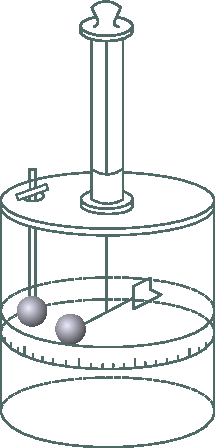
\includegraphics[scale=0.95]{figures/fig_1_1.pdf}
			\caption[]{}
			\label{fig:1_1}
		\end{center}
	\end{minipage}
	\hfill{ }%\hspace{-0.1cm}
	\begin{minipage}[t]{0.5\linewidth}
		\begin{center}
			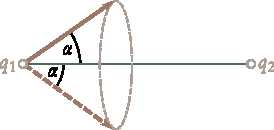
\includegraphics[scale=0.95]{figures/fig_1_2.pdf}
			\caption[]{}
			\label{fig:1_2}
		\end{center}
	\end{minipage}
%\vspace{-0.5cm}
\end{figure}

\begin{figure}[t]
	\begin{center}
		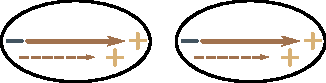
\includegraphics[scale=0.95]{figures/fig_1_3.pdf}
		\caption[]{}
		\label{fig:1_3}
	\end{center}
	\vspace{-0.8cm}
\end{figure}

Since when treating a body as a particle we ignore its length, the concept of circular motion about an axis passing through such a body cannot be applied to it.

To acquire the possibility of describing motion quantitatively, we have to associate a \textbf{coordinate system} (for example a Cartesian one) with the bodies forming a reference frame. Hence, the position of a particle can be determined by setting the three numbers $x$, $y$, and $z$---the Cartesian coordinates of the particle. A coordinate system can be made by forming a rectangular lattice from identical rods or rules graduated to a definite scale: (\fig{1_3}). Identical clocks synchronized with one another must be placed at the lattice points. The position of a particle and the moment of time corresponding to this position are recorded on the graduated rods and the clock closest to the particle.

It is simpler to treat a point particle than an extended body. We shall therefore first study the mechanics of a particle, and then go over to the mechanics of a rigid body. We shall start with kinematics, and then delve into dynamics. We remind our reader that \textbf{kinematics} studies the motion of bodies without regard to what causes this motion. \textbf{Dynamics} studies the motion of bodies with a view to what causes this motion to have the nature it does, \ie, with a view to the interactions between bodies.

\section{Vectors}\label{sec:1_2}

\textbf{Definition of a Vector.} Vectors are defined as quantities characterized by a numerical value and a direction and also as ones that are added according to the triangle or parallelogram method\footnote{According to a stricter definition, a vector is a combination of three quantities that transform when the coordinate axes rotate according to a definite law.}. The last requirement is a very significant one. We can indicate quantities characterized by a numerical value and a sense of direction but that are added in a different way than vectors. We shall take as an example the rotation of a body about an axis through the finite angle $\varphi$. Such rotation can be depicted in the form of a segment of length $\varphi$ directed along the axis about which rotation is occurring and pointing in a direction associated with that of rotation according to the right-hand screw rule. The top portion of \fig{1_4} shows two consecutive turns of the sphere through the angles $\pi/2$ depicted by the segments $\varphi_1$ and $\varphi_2$. The first turn about axis $1$---$1$ transfers point $A$ of the sphere to position $A'$, and the second turn about axis $2$---$2$ transfers it to position $A''$. The same result, \ie, transfer of point $A$ to position $A''$, can be achieved by turning the sphere about axis $3$---$3$ (see the bottom portion of \fig{1_4}) through the angle $\pi$. Hence, such a turn should be considered as the sum of the turns <p1 and <p 2 • It cannot be obtained from the segments $\varphi_1$ and $\varphi_2$, however, by adding them according to the parallelogram method. Such addition gives a segment of length $\pi/\sqrt{2}$ instead of the required length $\pi$. Rotation through the angle $\pi/\sqrt{2}$ transfers point $A$ to point $A'''$. It thus follows that the turns through finite angles depicted by the directed segments do not have the properties of vectors.

\begin{figure}[t]
	\begin{center}
		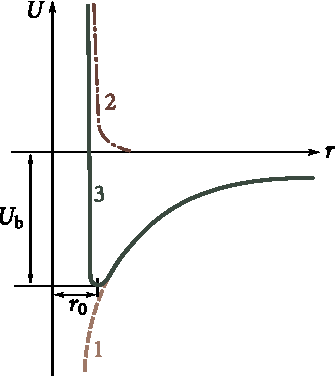
\includegraphics[scale=0.9]{figures/fig_1_4.pdf}
		\caption[]{}
		\label{fig:1_4}
	\end{center}
\vspace{-0.8cm}
\end{figure}

The numerical value of a vector is called its magnitude. Figuratively speaking, the magnitude of a vector indicates its length. The magnitude of a vector is a scalar, and always a positive one.

Vectors are represented graphically by arrows. The length of an arrow determines to the established scale the magnitude of the relevant vector, and the arrow points in the direction of the vector.

Vectors are customarily distinguished by setting their symbols in boldface type, for example, $\vec{a}$, $\vec{b}$, $\vec{v}$ and $\vec{F}$. The same symbols set in italics signify the magnitude of the relevant vectors, for example, $a$ is the magnitude of the vector $\vec{a}$\footnote{In handwriting, vectors are denoted by arrows over their symbols (for example, $\oldvec{a}$. In this case, the same letter without the arrow stands for the magnitude of the vector.}. It is sometimes necessary to express the magnitude by placing a vertical bar (an absolute value sign) on each side of the symbol for the vector. Thus, $|a|$ is the magnitude of the vector $\vec{a}$. This representation is used, for example, to show the magnitude of the sum of the vectors $\vec{a}_1$ and $\vec{a}_2$:
\begin{equation}\label{eq:1_1}
	|\vec{a}_1 + \vec{a}_2| = \text{magnitude of the vector } (\vec{a}_1 + \vec{a}_2).
\end{equation}

\noindent
In this case, the notation $a_1+a_2$ signifies the sum of the magnitudes of the vectors being added, which in general does not equal the magnitude of the sum of the vectors (the two sums will be equal only when the vectors being added have the same direction).

Vectors directed along parallel straight lines (in the same or in opposite directions) are called \textbf{collinear}. Vectors in parallel planes are called \textbf{coplanar}. Collinear vectors can be arranged along the same straight line and coplanar vectors can be brought into one plane by parallel translation.

Collinear vectors equal in magnitude and having the same direction are considered to equal each other\footnote{What is meant are the so-called \textbf{free vectors}, \ie, vectors that can be drawn from any point in space. Also distinguished are \textbf{slip vectors} whose tail can be placed at any point on the straight line along which the vector is directed, and localized vectors, which are applied to a definite point. The last two kinds of vectors can be expressed through free vectors. This is why vector calculus is based on the concept of the free vector, usually called simply a vector.}.

\textbf{Vector Addition and Subtraction.} It is more convenient to add vectors in practice without constructing a parallelogram. Examination of \fig{1_5} shows that we can achieve the same result if we bring the tail of the second vector in contact with the tip of the first one, and then draw the resultant vector from the tail of the first vector to the tip of the second one. It is very good to use this procedure when we have to add more than two vectors (\fig{1_6}).

\begin{figure}[t]
	\begin{minipage}[t]{0.5\linewidth}
		\begin{center}
			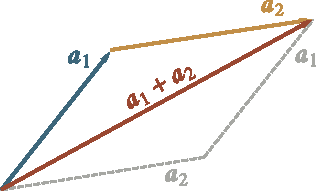
\includegraphics[scale=0.95]{figures/fig_1_5.pdf}
			\caption[]{}
			\label{fig:1_5}
		\end{center}
	\end{minipage}
	\hfill{ }%\hspace{-0.1cm}
	\begin{minipage}[t]{0.5\linewidth}
		\begin{center}
			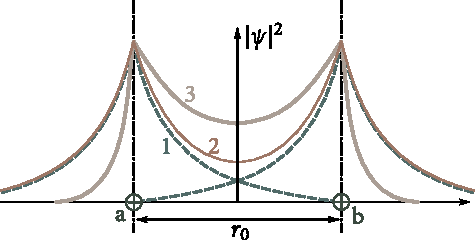
\includegraphics[scale=0.95]{figures/fig_1_6.pdf}
			\caption[]{}
			\label{fig:1_6}
		\end{center}
	\end{minipage}
\vspace{-0.7cm}
\end{figure}

The difference of two vectors $\vec{a}$ and $\vec{b}$ is defined as such a vector $\vec{c}$ which when added to the vector $\vec{b}$ gives the vector $\vec{a}$ (\fig{1_7}---the vector $-\vec{b}$ depicted by a dash line will be treated below The magnitude of the difference of two vectors, like the magnitude of a sum [see \eqn{1_1}], may be written only with the aid of vertical bars:
\begin{equation}\label{eq:1_2}
|\vec{a}_1 - \vec{a}_2| = \text{magnitude of the vector } (\vec{a}_1 - \vec{a}_2),
\end{equation}

\noindent
because the notation $a_1-a_2$ signifies the difference of the magnitudes of the vectors $\vec{a}_1$ and $\vec{a}_2$, which, generally speaking, does not equal the magnitude of the vector difference.

\textbf{Multiplication of a Vector by a Scalar.} Multiplication of the vector $\vec{a}$ by the scalar $\alpha$ yields a new vector $\vec{b}=\alpha\,\vec{a}$ whose magnitude is $|\alpha|$ times that of the vector a (\ie, $b=|\alpha|a$). The direction of the vector $\vec{b}$ either coincides with that of the vector $\vec{a}$ (if $\alpha>0$), or is opposite to it (if $\alpha<0$). It follows from the above that multiplication by $-1$ reverses the direction of a vector. Consequently, the vectors $\vec{a}$ and $-\vec{a}$ have the same magnitudes, but are opposite in direction. It is simple to see with the aid of  \fig{1_7} that subtraction of the vector $\vec{b}$ from the vector $\vec{a}$ is equivalent to addition of the vector $-\vec{b}$ to the vector $\vec{a}$.

It follows from our definition of multiplication of a vector by a scalar that any vector $\vec{a}$ can be represented in the form
\begin{equation}\label{eq:1_3}
\vec{a} = a\,\vecuni{a},
\end{equation} 

\noindent
where $a$ is the magnitude of the vector $\vec{a}$ and $\vecuni{a}$, is vector with a magnitude of unity and of the same direction as $\vec{a}$ (\fig{1_8}).

The vector $\vecuni{a}$ is called the unit vector of the vector $\vec{a}$. The unit vector can be represented in the form
\begin{equation}\label{eq:1_4}
\vecuni{a} = \frac{\vec{a}}{a},
\end{equation}

\noindent
whence it follows that it is a dimensionless quantity.

\begin{figure}[t]
	\begin{minipage}[t]{0.5\linewidth}
		\begin{center}
			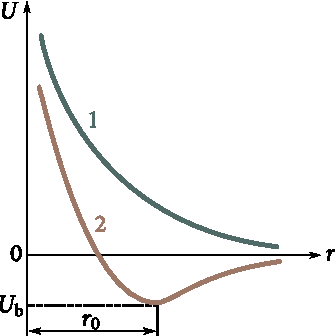
\includegraphics[scale=0.9]{figures/fig_1_7.pdf}
			\caption[]{}
			\label{fig:1_7}
		\end{center}
	\end{minipage}
	\hfill{ }%\hspace{-0.1cm}
	\begin{minipage}[t]{0.5\linewidth}
		\begin{center}
			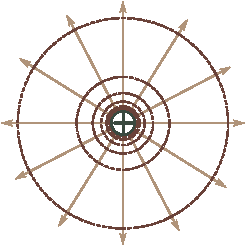
\includegraphics[scale=0.95]{figures/fig_1_8.pdf}
			\caption[]{}
			\label{fig:1_8}
		\end{center}
	\end{minipage}
\vspace{-0.6cm}
\end{figure}

Unit vectors can be compared not only with vectors, but also with any direction in space. For example, $\vecuni{x}$ is the unit vector of the coordinate axis $x$, $\vecuni{n}$ is the unit vector of a normal to a curve or surface, and $\vecuni{\tau}$ is the unit vector of a tangent to a curve.

\textbf{Linear Relation Between Vectors.} Let us consider three non-collinear vectors $\vec{a}$, $\vec{b}$ and $\vec{c}$ that are in one plane. A glance at \fig{1_9} shows that any of them (for instance, $\vec{c}$) can be expressed through the other two with the aid of the relation
\begin{equation}\label{eq:1_5}
\vec{c} = \alpha\vec{a} + \beta\vec{b},
\end{equation}

\noindent
where $\alpha$ and $\beta$ are scalars (for the case shown in the figure, $\alpha>1$ and $-1<\beta<0$). Hence, we conclude that any vector $\vec{c}$ that is in the same plane as the non-collinear vectors $\vec{a}$ and $\vec{b}$ can be expressed through the latter with the aid of linear relation~\eqref{eq:1_5}. When the vectors $\vec{a}$ and $\vec{b}$ are fixed, any third vector is unambiguously determined by the two quantities $\alpha$ and $\beta$.

Assume that we have three vectors $\vec{a}$, $\vec{b}$ and $\vec{c}$, each of which is not coplanar with the other two.\footnote{Two vectors are always coplanar. This follows from the fact that their tails can he made to coincide by translation, and they will thus be in one plane.} By analogy with \eqn{1_5}, we can see quite easily that any vector $\vec{d}$ can be represented as a linear combination of the given vectors:
\begin{equation}\label{eq:1_6}
\vec{d} = \alpha\vec{a} + \beta\vec{b} + \gamma\vec{c},
\end{equation}

\noindent
When the vectors $\vec{a}$, $\vec{b}$ and $\vec{c}$ are fixed, any vector $\vec{d}$ is unambiguously determined by the three quantities $\alpha$, $\beta$ and $\gamma$, each of which may be either positive or negative.

\textbf{Projection of a Vector.} Let us consider a direction in space that we shall set by the axis $l$ (\fig{1_10}). Let the vector $\vec{a}$ make the angle $\varphi$ with the axis $l$\footnote{If the straight line along which the vector $\vec{a}$ is directed and the axis $l$ do not intersect, the angle $\varphi$ should be found by drawing a straight line parallel to the vector $\vec{a}$ and intersecting the axis $l$. The angle between this line and the axis $l$ will be the angle $\varphi$ we are interested in.}. The quantity
\begin{equation}\label{eq:1_7}
a_l = a\, \cos\varphi
\end{equation}

\noindent
(where $a$ is the magnitude of the vector) is called the projection of the vector $\vec{a}$ onto the axis$l$. A projection is designated by the same symbol as its vector, with the addition of a subscript showing the direction onto which the vector has been projected. 

\begin{figure}[t]
	\begin{minipage}[t]{0.5\linewidth}
		\begin{center}
			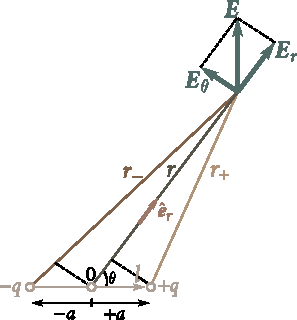
\includegraphics[scale=1]{figures/fig_1_9.pdf}
			\caption[]{}
			\label{fig:1_9}
		\end{center}
	\end{minipage}
	\hfill{ }%\hspace{-0.1cm}
	\begin{minipage}[t]{0.5\linewidth}
		\begin{center}
			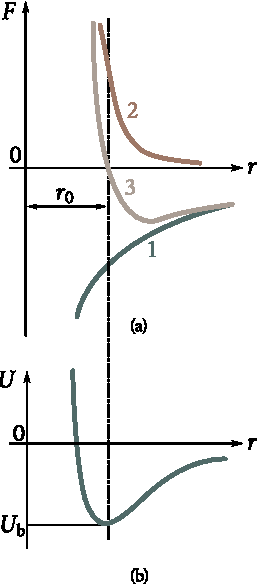
\includegraphics[scale=0.95]{figures/fig_1_10.pdf}
			\caption[]{}
			\label{fig:1_10}
		\end{center}
	\end{minipage}
	\vspace{-0.7cm}
\end{figure}

A projection of a vector is an algebraic quantity. If the vector makes an acute angle with the given direction, then $\cos\varphi>0$, and the projection is positive. If the angle $\varphi$ is obtuse, then $\cos\varphi<0$, and, consequently, the projection is negative. When a vector is at right angles to a given axis, its projection equals zero.

The projection of a vector has a simple geometrical meaning. It equals the distance between the projections of the tail and the tip of the segment depicting the given vector onto the given axis. When $\varphi<\pi/2$, this distance is assumed to be positive, and when $\varphi>\pi/2$, it is negative.

Let $\vec{a} = \vec{a}_1+\vec{a}_2+\vec{a}_3+\vec{a}_4$ (\fig{1_11}). It is easy to see from the figure that the projection of the resultant vector a onto a direction $l$ equals the sum of the projections of the separate vectors being added:
\begin{equation}\label{eq:1_8}
a_l = a_{1l}+a_{2l}+a_{3l}+a_{4l}.
\end{equation}

\noindent
We must remind our reader that when adding the projections of the vectors shown in \fig{1_11}, the distances $0$---$1$, $1$---$2$, and $2$---$3$ have to be taken with the plus sign, and the distance $3$---$4$ with the minus sign. Equation~\eqref{eq:1_8} holds for any number of addends.

\textbf{Expressing a Vector Through Its Projections onto the Coordinate Axes.} Let us take Cartesian coordinate axes and consider the vector $\vec{a}$ in a plane at right angles to the $z$-axis (\fig{1_12}). We shall introduce the unit vectors of the coordinate axes, \ie, the unit vectors $\vecuni{x}$, $\vecuni{y}$ and $\vecuni{z}$ ($\vecuni{z}$ is not shown in the drawing, it is perpendicular to the plane of the drawing and directed toward us). It must be noted that these three unit vectors completely determine a system of coordinates and are therefore called the \textbf{basis of the coordinate system}.

\begin{figure}[t]
	\begin{minipage}[t]{0.5\linewidth}
		\begin{center}
			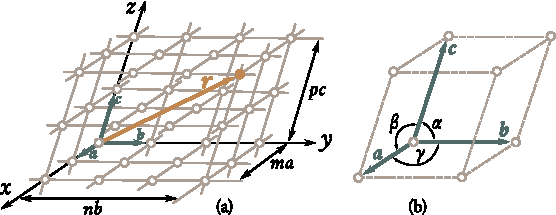
\includegraphics[scale=1]{figures/fig_1_11.pdf}
			\caption[]{}
			\label{fig:1_11}
		\end{center}
	\end{minipage}
	\hfill{ }%\hspace{-0.1cm}
	\begin{minipage}[t]{0.5\linewidth}
		\begin{center}
			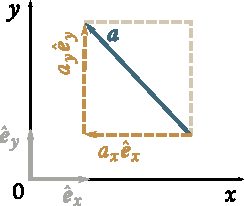
\includegraphics[scale=0.95]{figures/fig_1_12.pdf}
			\caption[]{}
			\label{fig:1_12}
		\end{center}
	\end{minipage}
	\vspace{-0.8cm}
\end{figure}

Inspection of \fig{1_12} shows that the vector $\vec{a}$ can be represented in the form of a linear combination of the unit vectors $\vecuni{x}$ and $\vecuni{y}$ [see \eqn{1_5}]:
\begin{equation*}
\vec{a} = a_x \vecuni{x} + a_y \vecuni{y}.
\end{equation*}

\noindent
The projections of the vector onto the coordinate axes play the part of the coefficients $\alpha$ and $\beta$. In the example being considered, the projection $a_x$ is negative, therefore the vector $a_x\vecuni{x}$ has a direction opposite to that of the unit vector $\vecuni{x}$.

We took the vector $\vec{a}$ perpendicular to the $z$-axis owing to which $a_z=0$. In the general case when all three projections of a vector differ from zero, we have
\begin{equation}\label{eq:1_9}
\vec{a} = a_x \vecuni{x} + a_y \vecuni{y} + a_z \vecuni{z},
\end{equation}

\noindent
Thus, any vector can be expressed through its projections onto the coordinate axes and the unit vectors of these axes. Therefore, the projections of a vector onto the coordinate axes are called its \textbf{components}.

The components $a_x$, $a_y$, $a_z$ equal (with an accuracy to the sign) the sides of a right parallelepiped in which the vector $\vec{a}$ is the major diagonal (\fig{1_13}). We therefore have
\begin{equation}\label{eq:1_10}
a^2 = a_x^2 + a_y^2 + a_z^2.
\end{equation}

Assume that $\vec{c}=\vec{a}+\vec{b}$. Representing each of these vectors in accordance with \eqn{1_9}, we get
\begin{equation*}
c_x\vecuni{x} + c_y\vecuni{y} + a_z\vecuni{z} = (a_x+b_x)\vecuni{x} + (a_y+b_y)\vecuni{y} + (a_z+b_z)\vecuni{z}
\end{equation*}

\noindent
(we have factored out $\vecuni{x}$, $\vecuni{y}$, and $\vecuni{z}$)· Equal vectors have identical projections onto the coordinate axes. On these grounds, we can write that
\begin{equation}\label{eq:1_11}
c_x=a_x+b_x,\quad c_y=a_y+b_y,\quad a_z=a_z+b_z
\end{equation}

\noindent
[compare with \eqn{1_8}]. Equations~\eqref{eq:1_11} express analytically the rule of vector addition. They hold for any number of addends.

\textbf{Position Vector.} The position vector (or radius vector) $\vec{r}$ of a point is defined as the vector drawn from the origin of coordinates to the given point (\fig{1_14}). Its projections onto the coordinate axes equal the Cartesian coordinates of the given point:
\begin{equation}\label{eq:1_12}
r_x=x,\quad r_y=y,\quad r_z=z.
\end{equation}

\noindent
Consequently, in accordance with \eqn{1_9}, the position vector can be represented in the form
\begin{equation}\label{eq:1_13}
\vec{r} = x\vecuni{x} + y\vecuni{y} + z\vecuni{z}.
\end{equation}

\noindent
By \eqn{1_10}, we have
\begin{equation}\label{eq:1_14}
r^2 = x^2 + y^2 + z^2.
\end{equation}

\begin{figure}[t]
	\begin{minipage}[t]{0.5\linewidth}
		\begin{center}
			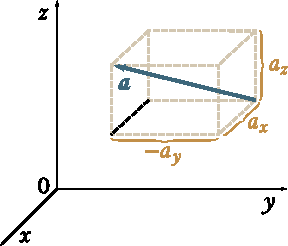
\includegraphics[scale=1]{figures/fig_1_13.pdf}
			\caption[]{}
			\label{fig:1_13}
		\end{center}
	\end{minipage}
	\hfill{ }%\hspace{-0.1cm}
	\begin{minipage}[t]{0.5\linewidth}
		\begin{center}
			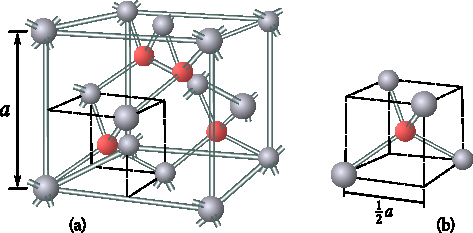
\includegraphics[scale=0.95]{figures/fig_1_14.pdf}
			\caption[]{}
			\label{fig:1_14}
		\end{center}
	\end{minipage}
\vspace{-0.3cm}
\end{figure}

\begin{figure}[t]
	\begin{center}
		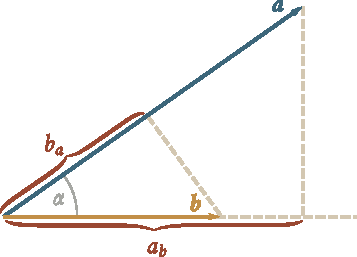
\includegraphics[scale=0.95]{figures/fig_1_15.pdf}
		\caption[]{}
		\label{fig:1_15}
	\end{center}
	\vspace{-1.0cm}
\end{figure}

\textbf{The Scalar Product of Vectors.} Two vectors $\vec{a}$ and $\vec{b}$ can be multiplied by each other in two ways. One of them results in a scalar quantity, and the other in a certain new vector. Accordingly, two products of vectors are distinguished---the scalar product and the vector product. It must be noted that \textit{the operation of dividing a vector by a vector does not exist}.

The scalar product of the vectors $\vec{a}$ and $\vec{b}$ is defined as the scalar quantity equal to the product of the magnitudes of these vectors and the cosine of the angle $\alpha$ between them:
\begin{equation}\label{eq:1_15}
\vecdot{a}{b} = ab\sin\alpha
\end{equation}

\noindent
(\fig{1_15}). When writing a scalar product, the symbols of the vectors being multiplied are usually written next to each other with dot between them (this is why a scalar product is also called a dot product; sometimes nothing is used between the symbols)\footnote{The dot symbol between vectors is preferred in the \LaTeX version to adopt a more modern approach.}. Equation~\eqref{eq:1_15} expresses an algebraic quantity: when $\alpha$ is acute, we have $\vecdot{a}{b}>0$, and when it is obtuse, we have $\vecdot{a}{b}<0$. The scalar product of mutually perpendicular vectors ($\alpha=\pi/2$) equals zero.

It must be noted that by the square of a vector is always meant the scalar product of this vector by itself:
\begin{equation}\label{eq:1_16}
\vec{a}^2 = \vecdot{a}{a} = aa\cos\alpha = a^2.
\end{equation}

\noindent
Thus, the square of a vector equals the square of its magnitude. In particular, the square of any unit vector equals unity:
\begin{equation}\label{eq:1_17}
\vecuni{x}^2 = \vecuni{y}^2 = \vecuni{z}^2 = 1.
\end{equation}

\noindent
We shall note in passing that owing to the unit vectors being mutually perpendicular, scalar products such as $\vecunidot{i}{k}$, equal zero if $i\neq k$.

The Kronecker symbol or delta $\delta_{ik}$ is very convenient. It is determined as follows:
\begin{equation}\label{eq:1_18}
\delta_{ik} = \begin{cases}
1, &\mbox{if } i = k, \\
0, &\mbox{if } i\neq k. \end{cases}
\end{equation}

\noindent
When this symbol is used, the properties of the scalar products of the coordinate axis unit vectors established above can be expressed by a single formula:
\begin{equation}\label{eq:1_19}
\vecunidot{i}{k} = \delta_{ik}\quad (i, k = x, y, z)
\end{equation}

\noindent
where the subscripts $i$ and $k$ can assume any of the values $x$, $y$ and $z$ independently of each other.

It follows from the definition~\eqref{eq:1_15} that a scalar product is commutative, \ie, it does not depend on the sequence of the multipliers:
\begin{equation}\label{eq:1_20}
\vecdot{a}{b} = \vecdot{b}{a}.
\end{equation}

\noindent
Equation~\eqref{eq:1_15} can be written in several ways:
\begin{equation*}
\vecdot{a}{b} = ab\cos\alpha = (a\cos\alpha)\,b = a\,(b\cos\alpha).
\end{equation*}

\noindent
Examination of \fig{1_15} shows that $a\cos\alpha$ equals $a_b$---the projection of the vector $\vec{a}$ onto the direction of the vector $\vec{b}$. Similarly, $b\cos\alpha= b_a$---the projection of the vector $\vec{b}$ onto the direction of the vector $\vec{a}$. We can therefore say that the scalar product of two vectors is defined as the scalar quantity equal to the product of the magnitude of one of the vectors being multiplied and the projection of the second vector onto the direction of the first one:
\begin{equation}\label{eq:1_21}
\vecdot{a}{b} = a_b b = a b_a.
\end{equation}

Taking into account that the projection of the sum of vectors equals the sum of the projections of the vectors being added, we can write that
\begin{equation}\label{eq:1_22}
\vec{a}\boldsymbol{\cdot}(\vec{b}+\vec{c}+\ldots) = a(\vec{b}+\vec{c}+\ldots)_a = a(b_a+c_a+\ldots) = ab_a+ac_a+\ldots = ab+ac+\ldots .
\end{equation}

\noindent
Hence, it follows that the scalar product of vectors is distributive---the product of the vector $\vec{a}$ and the sum of several vectors equals the sum of the products of the vector $\vec{a}$ and each of the added vectors taken separately.

Let us represent the vectors being multiplied in the form of \eqn{1_9} and take advantage of the distributive nature of a scalar product. We get
\begin{align*}
\vecdot{a}{b} &= (a_x\vecuni{x} + a_y\vecuni{y} + a_z\vecuni{z})(b_x\vecuni{x} + b_y\vecuni{y} + b_z\vecuni{z})\\
&= a_xb_x\vecunidot{x}{x} + a_xb_y\vecunidot{x}{y} + a_xb_z\vecunidot{x}{z} + a_yb_x\vecunidot{y}{x} + a_yb_y\vecunidot{y}{y}\\
&\,+ a_yb_z\vecunidot{y}{z}+ a_zb_x\vecunidot{z}{x} + a_zb_y\vecunidot{z}{y} + a_zb_z\vecunidot{z}{z}.
\end{align*}

\noindent
Now let us take \eqn{1_19} into consideration. As a result, we get an expression for a scalar product through the projections of the vectors being multiplied:
\begin{equation}\label{eq:1_23}
\vecdot{a}{b} = a_xb_x + a_yb_x + a_zb_z.
\end{equation}

\noindent
It must be noted that when the coordinate axes are rotated, the projections of vectors onto these axes change. The quantity $ab\cos\alpha$ does not depend on the choice of the axes, however. We thus conclude that the changes in the projections of the vectors $\vec{a}$ and $\vec{b}$, when the axes are rotated, are of a nature such that their combination of the form of \eqn{1_23} remains invariant (unchanged):
\begin{equation}\label{eq:1_24}
\vecdot{a}{b} = a_xb_x + a_yb_x + a_zb_z = \mathrm{inv}.
\end{equation}

It is a simple matter to see that the projection of the vector $\vec{a}$ onto the direction $l$ [see \eqn{1_7}] can be represented in the form
\begin{equation}\label{eq:1_25}
a_l = \vec{a}\boldsymbol{\cdot}\vecuni{l},
\end{equation}

\noindent
where $\vecuni{l}$ is the unit vector of the direction $l$. Similarly,
\begin{equation}\label{eq:1_26}
a_x = \vec{a}\boldsymbol{\cdot}\vecuni{x},\quad  a_y = \vec{a}\boldsymbol{\cdot}\vecuni{y}, \quad  a_z=\vec{a}\boldsymbol{\cdot}\vecuni{z}.
\end{equation}

\textbf{The Vector Product.} The vector product of the vectors $\vec{a}$ and $\vec{b}$ is defined as the vector $\vec{c}$ determined by the equation
\begin{equation}\label{eq:1_27}
\vec{c} = ab\sin(\alpha)\hatvec{n},
\end{equation}

\noindent
where $a$ y $b$ magnitudes of the vectors being multiplied, $\alpha$, is the angle between the vectors, $\hatvec{n}$, is the unit vector of a normal\footnote{The symbol $\hatvec{n}$ is simpler and more illustrative than $vecuni{n}$.} to the plane containing the vectors $\vec{a}$ and $\vec{b}$ (\fig{1_16}).

The direction of $\hatvec{n}$ is chosen so that the sequence of the vectors $\vec{a}$, $\vec{b}$, $\hatvec{n}$ forms a right-handed system. This signifies that if we look along the vector $\hatvec{n}$, then the shortest path in rotation from the first multiplier to the second one will be clockwise. In \fig{1_16}, the vector $\hatvec{n}$ is directed beyond the drawing, and it is therefore depicted by a circle with a cross\footnote{We shall depict vectors perpendicular to the plane of a drawing by a circle with a cross in it if the vector is directed away from us, and by a circle with a point at its centre if the vector is directed toward us. For clarity, we can imagine a vector in the form of an arrow with a tapered tip and cross-shaped feathers on its tail. Thus, when the vector is directed toward us (the arrow is flying toward us), we see a circle with a point; when the vector is directed away from us (the arrow is flying away from us), we see a circle with a cross.}. The direction of the vector $\vec{c}$ coincides with that of $\hatvec{n}$.

%\begin{figure}[t]
%	\begin{center}
%		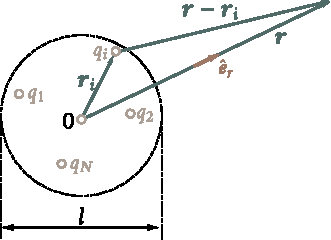
\includegraphics[scale=1]{figures/fig_1_16.pdf}
%		\caption[]{}
%		\label{fig:1_16}
%	\end{center}
%	\vspace{-0.7cm}
%\end{figure}

A vector product is usually designated in one of two ways:
\begin{equation*}
[\vec{a},\vec{b}]\quad\text{or }\quad \vec{a}\times\vec{b}
\end{equation*}

\noindent
the latter notation resulting in the term cross product sometimes being used to signify a vector product. We shall use the latter notation\footnote{To avoid confusion, in the \LaTeX version, we shall use the cross product symbol.}. Thus, according to \eqn{1_27}, we have
\begin{equation}\label{eq:1_28}
\vecprod{a}{b} = (ab\sin\alpha)\hatvec{n}.
\end{equation}

A glance at \fig{1_16} shows that the magnitude of a vector product has a simple geometrical meaning---the expression $ab\sin\alpha$ numerically equals the area of a parallelogram constructed on the vectors being multiplied.

We determined the direction of the vector $\vecprod{a}{b}$ by relating it to the direction of rotation from the first multiplier to the second one. When considering vectors such as the position vector $\vec{r}$, the velocity $\vec{v}$, and the force $\vec{F}$, the choice of their direction is quite obvious---it follows from the nature of these quantities themselves. Such vectors are called \textbf{polar} or \textbf{true}. Vectors of the type $\vecprod{a}{b}$ whose direction is related to that of rotation are called axial or \textbf{pseudovectors}. When conditions change, for example, upon going over from a right-hand system of coordinates to a left-hand one, the directions of pseudovectors are reversed, while those of true vectors remain unchanged.

It must be borne in mind that a vector product will be a pseudovector only when both of the vectors being multiplied are true (or both are pseudovectors). The vector product of a true vector and a pseudovector will be true. Reversing of a condition determining the direction of a pseudovector will lead in this case to a change in the sign in front of the vector product and also to a change in the sign of one of the multipliers. As a result, the quantity expressed
by the vector product remains unchanged.

Since the direction of a vector product is determined by the direction of rotation from the first multiplier to the second one, the result of vector multiplication depends on the order of the multipliers. Transposition of the multipliers leads to reversing of the direction of the resultant vector. Thus, a vector product does not have the property of commutativity:
\begin{equation}\label{eq:1_29}
\vecprod{a}{b} = -\vecprod{b}{a}.
\end{equation}

\noindent
A vector product can be proved to be distributive, \ie, it can be shown that
\begin{equation}\label{eq:1_30}
\vec{a}\times(\vec{b}_1+\vec{b}_2+\ldots)] = \vec{a}\times\vec{b}_1 + \vec{a}\times\vec{b}_2 + \ldots.
\end{equation}

%\begin{figure}[t]
%	\begin{center}
%		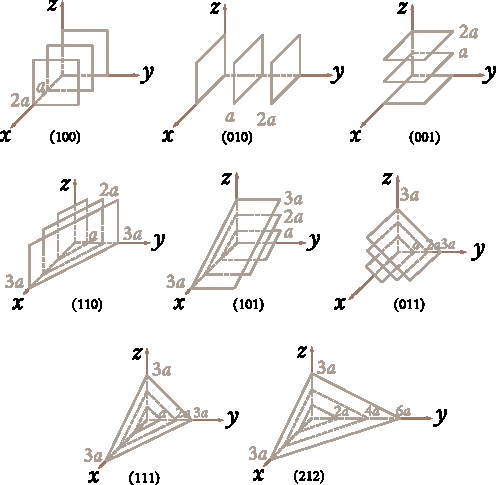
\includegraphics[scale=1]{figures/fig_1_17.pdf}
%		\caption[]{}
%		\label{fig:1_17}
%	\end{center}
%	\vspace{-1.0cm}
%\end{figure}
\begin{figure}[t]
	\begin{minipage}[t]{0.5\linewidth}
		\begin{center}
			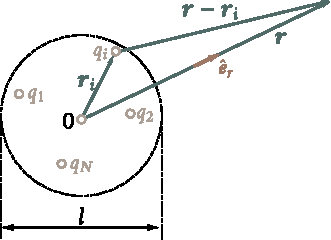
\includegraphics[scale=1]{figures/fig_1_16.pdf}
			\caption[]{}
			\label{fig:1_16}
		\end{center}
	\end{minipage}
	\hfill{ }%\hspace{-0.1cm}
	\begin{minipage}[t]{0.5\linewidth}
		\begin{center}
			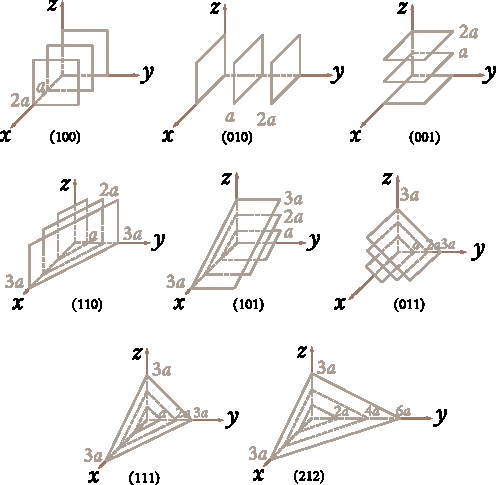
\includegraphics[scale=1]{figures/fig_1_17.pdf}
			\caption[]{}
			\label{fig:1_17}
		\end{center}
	\end{minipage}
	\vspace{-0.3cm}
\end{figure}

Let us consider the vector products of the unit vectors of the coordinate axes (\fig{1_17}). In accordance with the definition~\eqref{eq:1_28}, we have
\begin{align}
\vecuniprod{x}{x} &= \vecuniprod{y}{y} = \vecuniprod{z}{z} = 0,\nonumber\\
\vecuniprod{x}{y} &= -\vecuniprod{y}{x} = \vecuni{z},\label{eq:1_31}\\
\vecuniprod{y}{z} &= -\vecuniprod{z}{y} = \vecuni{x},\nonumber\\
\vecuniprod{z}{x} &= -\vecuniprod{x}{z} = \vecuni{y}.\nonumber
\end{align}

\noindent
Representing the vectors being multiplied in the form of \eqn{1_9} and taking advantage of the distributivity of a vector product, we get:
\begin{align*}
\vecprod{a}{b} &= (a_x\vecuni{x}+a_y\vecuni{y}+a_z\vecuni{z})\times(b_x\vecuni{x}+b_y\vecuni{y}+b_z\vecuni{z})\\
&= a_xb_x\vecuniprod{x}{x} + a_xb_y\vecuniprod{x}{y} + a_xb_z\vecuniprod{x}{z}\\
&+ a_yb_x\vecuniprod{y}{x} + a_yb_y\vecuniprod{y}{y} + a_yb_z\vecuniprod{y}{z}\\
&+ a_zb_x\vecuniprod{z}{x} + a_zb_y\vecuniprod{z}{y} + a_zb_z\vecuniprod{z}{z}
\end{align*}

\noindent
Taking into account relation~\eqref{eq:1_31}, we arrive at the following expression:
\begin{equation}\label{eq:1_32}
\vecprod{a}{b} = \vecuni{x}(a_yb_z - a_zb_y) + \vecuni{y}(a_zb_x - a_xb_z) + \vecuni{z}(a_xb_y - a_yb_x).
\end{equation}

\noindent
The above expression can be represented in the form of a determinant
\begin{equation}\label{eq:1_33}
\vecprod{a}{b} = \begin{vmatrix}
\vecuni{x} & \vecuni{y} & \vecuni{z}\\
a_x & a_y & a_z\\
b_x & b_y & b_z
\end{vmatrix}.
\end{equation}

\begin{figure}[t]
	\begin{center}
		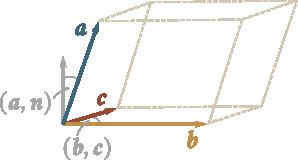
\includegraphics[scale=1]{figures/fig_1_18.pdf}
		\caption[]{}
		\label{fig:1_18}
	\end{center}
	\vspace{-0.7cm}
\end{figure}

\textbf{Scalar Triple Product.} A scalar triple product of three vectors is defined as the expression $\vecmix{a}{b}{c}$, \ie, the scalar product of the vector $\vec{a}$ and the vector product of the vectors $\vec{b}$ and $\vec{c}$. According to the definitions~\eqref{eq:1_15} and~\eqref{eq:1_28}, we have
\begin{equation*}
\vecmix{a}{b}{c} = a\{bc\sin(\vec{b}, \vec{c})\}\cos(\vec{a},\hatvec{n}).
\end{equation*}

\noindent
Here $(\vec{b},\vec{c})$ is the angle between $\vec{b}$ and $\vec{c}$, and $(\vec{a},\hatvec{n})$ is the angle between the vector $\vec{a}$ and the unit vector $\hatvec{n}$ determining the direction of the vector $\vecprod{b}{c}$. Inspection of \fig{1_18} shows that the expression $bc\sin(\vec{b},\vec{c})$ numerically equals the area of the base of a parallelepiped constructed on the vector being multiplied, while the expression $a\cos(\vec{a},\hatvec{n})$ numerically equals the altitude of this parallelepiped taken with the plus sign if the angle $(\vec{a},\hatvec{n})$ is acute, and with the minus sign if it is obtuse. Consequently, the expression $\vecmix{a}{b}{c}$ has a simple geometrical meaning---it numerically equals the volume of a parallelepiped constructed on the vectors being multiplied [taken with the plus or minus sign depending on the value of the angle $(\vec{a},\hatvec{n})$]. In calculating the volume of a parallelepiped, the result cannot depend on which of its faces is taken as the base. Hence, it follows that
\begin{equation}\label{eq:1_34}
\vecmix{a}{b}{c} = \vecmix{b}{c}{a} = \vecmix{c}{a}{b}.
\end{equation}

\noindent
Thus, a scalar triple product permits cyclic transposition of the multipliers, \ie, substitution for each of the multipliers of the one following it in the cycle:
\begin{equation*}
\begin{tikzcd}
\vec{a}\arrow[rd] &\\
\vec{c}\arrow[u] & \arrow[l] \vec{b}
\end{tikzcd}
\end{equation*}

\textbf{Vector Triple Product.} Let us consider a vector triple product of the three vectors $\vec{a}$, $\vec{b}$ and $\vec{c}$
\begin{equation*}
\vec{d} = \vec{a}\times\vecprod{b}{c}.
\end{equation*}

\noindent
Any vector product is perpendicular to both multipliers. Therefore, the vector $\vec{d}$ is perpendicular to the unit vector $\hatvec{n}$ determining the direction of the vector $\vecprod{b}{c}$. Hence, it follows that the vector $\vec{d}$ is in the plane formed by the vectors $\vec{b}$ and $\vec{c}$ and, consequently, can be represented as a linear combination of these vectors:
\begin{equation*}
\vec{d} = \alpha\vec{b} + \beta\vec{c}
\end{equation*}

\noindent
[see \eqn{1_5}]. We find from the relevant calculations that $\alpha=\vecdot{a}{c}$ and $\beta=-\vecdot{a}{b}$. Thus,
\begin{equation}\label{eq:1_35}
\vec{a}\times\vecprod{b}{c} = \vec{b}(\vecdot{a}{c}) - \vec{c}(\vecdot{a}{b}).
\end{equation}

\textbf{Derivative of a Vector.} Let us consider a vector that changes in time according to a known law $\vec{a}(t)$. The projections of this vector onto the coordinate axes are preset functions of time. Hence,
\begin{equation}\label{eq:1_36}
\vec{a}(t) = \vecuni{x}a_x(t) + \vecuni{y}a_y(t) + \vecuni{z}a_z(t)
\end{equation}

\noindent
(we assume that the coordinate axes do not rotate in space so that their unit vectors do not change with time).

Let the vector projections receive the increments $\Delta a_x$, $\Delta a_y$, $\Delta a_z$ during the time $\Delta t$. The vector therefore receives the increment $\Delta\vec{a} = \vecuni{x}\Delta a_x + \vecuni{y}\Delta a_y + \vecuni{z}\Delta a_z$. The rate of change of the vector $\vec{a}$ with time can be characterized by the ratio of $\Delta\vec{a}$ to $\Delta t$:
\begin{equation}\label{eq:1_37}
\frac{\Delta\vec{a}}{\Delta t} = \vecuni{x}\frac{\Delta a_x}{\Delta t} + \vecuni{y}\frac{\Delta a_y}{\Delta t} + \vecuni{z}\frac{\Delta a_z}{\Delta t}.
\end{equation}

\noindent
This expression gives the mean rate of change of $\vec{a}$ during the time interval $\Delta t$. Let us assume that $\vec{a}$ changes continuously with time, without any jumps. Consequently, the smaller the interval $\Delta t$, the more accurately does the value of \eqn{1_37} characterize the rate of change in $\vec{a}$ at the moment $t$ preceding the interval $\Delta t$. Therefore, the rate of change in the vector $\vec{a}$ at the moment $t$ equals the limit of \eqn{1_37} obtained when $\Delta t$ tends to zero:
\begin{align}
\text{the rate of change in }\vec{a} &= \lim_{\Delta t\to 0}\frac{\Delta\vec{a}}{\Delta t} \nonumber\\
&= \vecuni{x} \lim_{\Delta t\to 0}\frac{\Delta a_x}{\Delta t} + \lim_{\Delta t\to 0}\vecuni{y} \frac{\Delta a_y}{\Delta t} + \lim_{\Delta t\to 0}\vecuni{z} \frac{\Delta a_z}{\Delta t}.\label{eq:1_38}
\end{align}

If there is a function $f(t)$ of the argument $t$, then the limit of the ratio of the increment of the function $\Delta f$ to the increment of the argument $\Delta t$ obtained when $\Delta t$ tends to zero is called the derivative of the function $f$ with respect to $t$ and is designated by the symbol $\diffin{f}{t}$. Expression~\eqref{eq:1_38} can therefore be written as follows:
\begin{equation}\label{eq:1_39}
\diff{\vec{a}}{t} = \vecuni{x}\diff{a_x}{t} + \vecuni{y}\diff{a_y}{t} + \vecuni{z}\diff{a_z}{t}.
\end{equation}

\noindent
The result obtained signifies that the projections of the vector $\diffin{\vec{a}}{t}$ onto the coordinate axes equal the time derivatives of the projections of the vector $\vec{a}$:
\begin{equation}\label{eq:1_40}
\left(\diff{\vec{a}}{t}\right)_{\text{pr. }x} = \diff{a_x}{t},\quad \left(\diff{\vec{a}}{t}\right)_{\text{pr. }y} = \diff{a_y}{t},\quad \left(\diff{\vec{a}}{t}\right)_{\text{pr. }z} = \diff{a_z}{t},\quad.
\end{equation}

It is customary practice in physics to denote time derivatives by the symbol of the corresponding quantity with a dot over it, for example,
\begin{equation}\label{eq:1_41}
\diff{\varphi}{t} = \dot{\varphi},\quad \diffsec{\varphi}{t} = \ddot{\varphi},\quad \diff{\vec{a}}{t} = \dot{\vec{a}},\quad \diffsec{\vec{a}}{t} = \ddot{\vec{a}}.
\end{equation}

\noindent
Using this notation, we can write equation~\eqref{eq:1_39} as follows:
\begin{equation}\label{eq:1_42}
\dot{\vec{a}} = \vecuni{x}\dot{a}_x + \vecuni{y}\dot{a}_y + \vecuni{z}\dot{a}_z.
\end{equation}

\noindent
If we take the position vector $\vec{r}(t)$ of a moving point as $\vec{a}(t)$, then by \eqn{1_42} we have
\begin{equation}\label{eq:1_43}
\dot{\vec{r}} = \vecuni{x}\dot{r}_x + \vecuni{y}\dot{r}_y + \vecuni{z}\dot{r}_z,
\end{equation}

\noindent
where $x$, $y$, $z$ are functions of $t$, namely, $x=x(t)$, $y=t(t)$, $z=z(t)$.

The differential (``increment'') of the function $f(t)$ is defined as the expression
\begin{equation}\label{eq:1_44}
\mathrm{d}f = f'\, \mathrm{d}t,
\end{equation}

\noindent
where $f'$ is the derivative of $f$ with respect to $t$.  According to \eqn{1_39}, the differential of the vector $\vec{a}$ is determined by the equation
\begin{equation}\label{eq:1_45}
\mathrm{d}\vec{a} = \vecuni{x}\mathrm{d}a_x + \vecuni{y}\mathrm{d}a_y + \vecuni{z}\mathrm{d}a_z.
\end{equation}

In particular,
\begin{equation}\label{eq:1_46}
\mathrm{d}\vec{r} = \vecuni{x}\mathrm{d}x + \vecuni{y}\mathrm{d}y + \vecuni{z}\mathrm{d}z.
\end{equation}

It must be noted that the increment of a function during a very short, but finite interval $\Delta t$ approximately equals
\begin{equation}\label{eq:1_47}
\Delta f \approx f'\Delta t = \diff{f}{t}\Delta t.
\end{equation}

\noindent
In the limit, when $\Delta t\to 0$, the approximate equation~\eqref{eq:1_47} transforms into the accurate equation~\eqref{eq:1_44}.

A similar equation to~\eqref{eq:1_47} can also be written for the vector function
\begin{equation}\label{eq:1_48}
\Delta\vec{a} \approx \diff{\vec{a}}{t}\Delta t.
\end{equation}

\textbf{Derivative of the Product of Functions.} We shall consider the function $\vec{b}(t)$ that equals the product of the scalar function $\varphi(t)$ and the vector function $\vec{a}(t)$, \ie, $\vec{b}(t)=\varphi(t)\vec{a}(t)$ or, more briefly, $\vec{b}=\varphi\vec{a}$. Let us find the increment of the function $\vec{b}$:
\begin{equation*}
\Delta\vec{b} = \Delta(\varphi\vec{a}) = (\varphi + \Delta\varphi)(\vec{a} + \Delta\vec{a}) - \varphi\vec{a} = \varphi\Delta\vec{a} + \vec{a}\Delta\varphi + \Delta\varphi\Delta\vec{a}.
\end{equation*}

\noindent
Representing the increments of the functions in the form of expressions~\eqref{eq:1_47} and~\eqref{eq:1_48}, we get:
\begin{equation*}
\Delta\vec{b} \approx \varphi\diff{\vec{a}}{t}\Delta t + \vec{a}\diff{\varphi}{t}\Delta t + \diff{\varphi}{t}\diff{\vec{a}}{t}(\Delta t)^2
\end{equation*}

\noindent
whence
\begin{equation*}
\frac{\Delta\vec{b}}{\Delta t} \approx \varphi\diff{\vec{a}}{t} + \vec{a}\diff{\varphi}{t} + \diff{\varphi}{t}\diff{\vec{a}}{t}\Delta t.
\end{equation*}

\noindent
In the limit when $\mathrm{d}t$ tends to zero, this approximate equation transforms into an accurate one. Thus,
\begin{equation*}
\diff{\vec{b}}{t} = \lim_{\Delta t\to 0} \diff{\vec{b}}{t} =  \lim_{\Delta t\to 0} \left(\varphi\diff{\vec{a}}{t} + \vec{a}\diff{\varphi}{t} + \diff{\varphi}{t} \diff{\vec{a}}{t}\Delta t\right).
\end{equation*}

\noindent
The first two addends do not depend on $\Delta t$ and therefore do not change when going over to the limit. The limit of the third addend equals zero. Hence, substituting $\varphi\vec{a}$ for $\vec{b}$, we obtain
\begin{equation}\label{eq:1_49}
\diff{(\varphi\vec{a})}{t} = \varphi\diff{\vec{a}}{t} + \vec{a}\diff{\varphi}{t} = \varphi\dot{\vec{a}}+\dot{\varphi}\vec{a}.
\end{equation}

Now let us consider the scalar product of two vector functions $\vec{a}(t)$ and $\vec{b}(t)$. The increment of this product is
\begin{align*}
\Delta(\vec{a}\vec{b}) &= (\vec{a} + \Delta\vec{a})(\vec{b} + \Delta\vec{b}) - \vec{a}\vec{b}\\
&= \vec{a}\Delta\vec{b} + \vec{b}\Delta\vec{a} + \Delta\vec{a}\Delta\vec{b} \\
&\approx \vec{a}\dot{\vec{b}}\Delta t + \vec{b}\dot{\vec{a}}\Delta t + \dot{\vec{a}}\dot{\vec{b}}(\Delta t)^2
\end{align*}

\noindent
Hence
\begin{equation*}
\diff{(\vec{a}\vec{b})}{t} = \lim_{\Delta t\to 0} \frac{\Delta(\vec{a}\vec{b})}{\Delta t} = \lim_{\Delta t\to 0} (\vec{a}\dot{\vec{b}} + \vec{b}\dot{\vec{a}} + \dot{\vec{a}}\dot{\vec{b}}\Delta t)
\end{equation*}

\noindent
or finally
\begin{equation}\label{eq:1_50}
\diff{(\vec{a}\vec{b})}{t} = \vec{a}\dot{\vec{b}} + \vec{b}\dot{\vec{a}}.
\end{equation}

\noindent
Multiplying \eqn{1_50} by $\mathrm{d}t$, we get a differential:
\begin{equation}\label{eq:1_51}
\diff{(\vec{a}\vec{b})}{t} = \vec{a}\dot{\vec{b}} + \vec{b}\dot{\vec{a}}.
\end{equation}

Let us calculate the derivative and the differential of the square of a vector function. According to Eqs.~\eqref{eq:1_50} and~\eqref{eq:1_51}, we have
\begin{align}
\diff{\vec{a}^2}{t} &= 2\vec{a}\dot{\vec{a}},\label{eq:1_52}\\
\mathrm{d}(\vec{a}^2) &= 2\vec{a}\,\mathrm{d}\vec{a},\label{eq:1_53}
\end{align}

\noindent
Taking into account that $\vec{a}^2 = a^2$ [see \eqn{1_16}], we can write:
\begin{equation}\label{eq:1_54}
2\vec{a}\,\mathrm{d}\vec{a} = \mathrm{d}(a^2) \quad \text{or} \quad \vec{a}\,\mathrm{d}\vec{a} = \mathrm{d}\left(\frac{a^2}{2}\right).
\end{equation}

Finally, let us consider the derivative of the vector product of the functions $\vec{a}(t)$ and $\vec{b}(t)$. The increment of the function being considered is
\begin{align*}
\Delta\vecprod{a}{b} &= [(\vec{a} + \Delta\vec{a}),(\vec{b} + \Delta\vec{b}) - \vecprod{a}{b}]\\
&= [\vec{a},\Delta\vec{b}] + [\Delta\vec{a},\vec{b}] + [\Delta\vec{a},\Delta\vec{b}]\\
&\approx [\vec{a},\dot{\vec{b}}\Delta t] + [\dot{\vec{a}}\Delta t,\vec{b}] + [\dot{\vec{a}}\Delta t,\dot{\vec{b}}\Delta t].
\end{align*}

\noindent
Correspondingly,
\begin{equation*}
\diff{\vecprod{a}{b}}{t} = \lim_{\Delta t\to 0} \{[\vec{a},\dot{\vec{b}}] + [\dot{\vec{a}},\vec{b}] + [\dot{\vec{a}},\dot{\vec{b}}]\Delta t\}.
\end{equation*}

\noindent
After a limit transition, we arrive at the equation
\begin{equation}\label{eq:1_55}
\diff{\vecprod{a}{b}}{t} = [\vec{a},\dot{\vec{b}}] + [\dot{\vec{a}},\vec{b}].
\end{equation}

\textbf{Derivative of a Unit Vector.} Let us consider the unit vector $\vecuni{a}$ of the vector $\vec{a}$. It is obvious that the vector $\vecuni{a}$ can change only in direction. Assume that during the very short interval $\Delta t$ the vector $\vec{a}$ and together with it the unit vector $\vecuni{a}$ rotate through the angle $\Delta\varphi$ (\fig{1_19}). At a low value of $\Delta\varphi$, the magnitude of the vector $\Delta\vecuni{a}$ approximately equals the angle $\Delta\varphi$, namely, $|\Delta\vecuni{a}|\approx\Delta\varphi$ (the segment depicting $\Delta\vecuni{a}$ is the base of an isosceles triangle with sides equal to unity). We must note that the smaller is $\Delta\varphi$, the more accurate is our approximate equation. The vector $\Delta\varphi$ itself can be represented in the form 
\begin{equation*}
\Delta\vecuni{a} = |\Delta\vecuni{a}| \boldsymbol{\cdot} \vecuni{\Delta\vec{e}} \approx \Delta\varphi \boldsymbol{\cdot} \vecuni{\Delta\vec{e}}
\end{equation*}

\noindent
where $\vecuni{\Delta\vec{e}}$ is the unit vector of the vector $\Delta\vecuni{a}$. When $\Delta\varphi$ tends to zero, the unit vector $\vecuni{\Delta\vec{e}}$ will rotate and in the limit coincide with the unit vector $\vecuni{\perp}$ perpendicular to $\vecuni{a}$ (see \fig{1_19}).

The derivative of $\vecuni{a}$ with respect to $t$, by definition, is
\begin{equation*}
\diff{\vecuni{a}}{t} = \lim_{\Delta t\to 0} \frac{\Delta\vecuni{a}}{\Delta t} = \lim_{\Delta t\to 0} \frac{\Delta\varphi}{\Delta t}\vecuni{\Delta\vec{e}} = \diff{\varphi}{t}\vecuni{\perp}.
\end{equation*}

\noindent
Thus,
\begin{equation}\label{eq:1_56}
\dot{\hat{\vec{e}}}_{a} = \dot{\varphi}\vecuni{\perp}.
\end{equation}

\noindent
The quantity $\dot{\varphi}=\diffin{\varphi}{t}$ is the angular velocity of rotation of the vector $\vec{a}$ (see Sec.~\ref{sec:1_5}). The unit vector $\vecuni{\perp}$ is in the plane in which the vector $\vec{a}$ is rotating at the given moment, and its sense is in the direction of rotation.

\begin{figure}[t]
	\begin{center}
		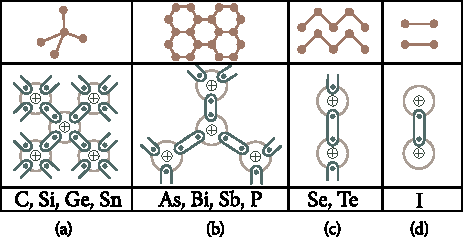
\includegraphics[scale=0.95]{figures/fig_1_19.pdf}
		\caption[]{}
		\label{fig:1_19}
	\end{center}
	\vspace{-0.7cm}
\end{figure}

\section{Velocity and Speed}\label{sec:1_3}

A point particle in motion travels along a certain line. The latter is called its path or trajectory\footnote{It must be noted that the concept of a trajectory can be applied only to a ``classical'' particle to which accurate values of its coordinate and momentum (\ie, velocity) can be ascribed at each moment of time. According to quantum mechanics, real particles can be characterized with the aid of a coordinate and momentum only with a certain accuracy. The limit of this accuracy is determined by the equation of Heisenberg's uncertainty principle: $\Delta x\Delta p\gtrsim\hbar$. Here $\Delta x$ is the uncertainty in the coordinate of a particle, $\Delta p$ is the uncertainty in its momentum, and $\hbar$ is Planck's constant $h$ divided by $2\pi$, \ie, $\hbar = h/2\pi = \SI{1.05e-34}{\joule\second}$. The sign $\gtrsim$ signifies ``greater than a value of the order of''. Replacing the momentum with the product of the mass and the velocity, we can write $\Delta x\Delta v\gtrsim\hbar/m$. It can be seen from this relation that the smaller the mass of a particle, the more uncertain do its coordinate and velocity become, and, consequently, the less applicable is the concept of trajectory. For macroscopic bodies (\ie, bodies formed by a very great number of molecules), the uncertainties in the coordinate and velocity do not exceed the practically attainable accuracy of measuring these quantities. Hence, the concept of trajectory may be applied to such bodies without any reservations. For microparticles (electrons, protons, neutrons, separate atoms and molecules), the concept of trajectory either cannot be applied at all, or can be applied with a limited accuracy, depending on the conditions in which motion occurs. For example, the motion o electrons in a cathode-ray tube can approximately be considered as occurring along certain trajectories.}. Depending on the shape of a trajectory, we distinguish rectilinear or straight motion, circular motion, curvilinear motion, etc.

\begin{figure}[t]
	\begin{minipage}[t]{0.5\linewidth}
		\begin{center}
			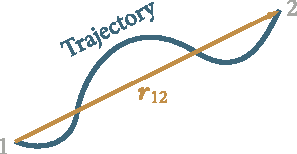
\includegraphics[scale=0.95]{figures/fig_1_20.pdf}
			\caption[]{}
			\label{fig:1_20}
		\end{center}
	\end{minipage}
	\hfill{ }%\hspace{-0.1cm}
	\begin{minipage}[t]{0.5\linewidth}
		\begin{center}
			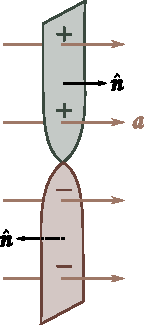
\includegraphics[scale=0.95]{figures/fig_1_21.pdf}
			\caption[]{}
			\label{fig:1_21}
		\end{center}
	\end{minipage}
%	\vspace{-0.7cm}
\end{figure}

Assume that a point particle (in the following we shall call it simply a particle for brevity's sake) travelled along a certain trajectory from point $1$ to point $2$ (\fig{1_20}). The path between points $1$ and $2$ measured along the trajectory is called the distance travelled by the particle. We shall denote it by the symbol $s$.

The straight line between points $1$ and $2$, \ie, the shortest distance between these points, is called the displacement of the particle. We shall denote it by the symbol $\vec{r}_{12}$. Let us assume that a particle completes two successive displacements $\vec{r}_{12}$ and $\vec{r}_{23}$ (\fig{1_21}). It is natural to call such a displacement $\vec{r}_{13}$ the sum of the first two that leads to the same result as they do together. Thus, displacements are characterized by magnitude and direction and, besides, are added by using the parallelogram method. Hence, it follows that displacement is a vector.

In everyday life, we use the terms \textbf{speed} and \textbf{velocity} interchangeably, but in physics there is an important distinction between them. Speed depends on the distance travelled, and velocity on the displacement. Speed is the distance travelled by a particle in unit time. If a particle travels identical distances during equal time intervals that may be as small as desired, its motion is called uniform. In this case, the speed of the particle at each moment can be calculated by dividing the distance $s$ by the time $t$.

Velocity is a vector quantity characterizing not only how fast a particle travels along its trajectory, but also the direction in which the particle moves at each moment. Let us divide a trajectory into infinitely small portions of length $\mathrm{d}s$. An infinitely small displacement $\mathrm{d}r$ corresponds to each of these portions (\fig{1_22}). Dividing this displacement by the corresponding time interval $\mathrm{d}t$, we get the instantaneous velocity at the given point of the trajectory:
\begin{equation}\label{eq:1_57}
\vec{v} = \diff{\vec{r}}{t} = \dot{\vec{r}}.
\end{equation}

\noindent
Thus, the velocity is the derivative of the position vector of the particle with respect to time. The displacement $\mathrm{d}r$ coincides with an infinitely small element of the trajectory. Consequently, the vector $\vec{v}$ is directed along a tangent to the trajectory (see \fig{1_22}).

\begin{figure}[t]
	\begin{center}
		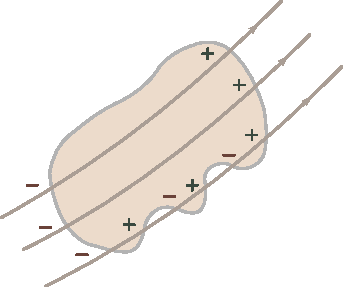
\includegraphics[scale=0.9]{figures/fig_1_22.pdf}
		\caption[]{}
		\label{fig:1_22}
	\end{center}
\vspace{-0.7cm}
\end{figure}

Reasoning more strictly, to derive equation~\eqref{eq:1_57} we must proceed as follows.· Having fixed a certain moment of time $t$, let us consider the increment of the position vector $\Delta\vec{r}$ during the small time interval $\Delta t$\footnote{The symbol $\Delta$ (delta) is used in two cases: (a) for designating the increment of a quantity. In the case being considered, $\Delta\vec{r}$ is the increment of the position vector $\vec{r}$ during the time $\Delta t$; (b) for designating a fraction of a quantity. For example, $\Delta t$ is a fraction of the total time $t$ during which motion occurs, and $\Delta s$ is a fraction of the entire 	distance $s$ travelled by the particle.} following $t$ (\fig{1_23}). The ratio $\Delta\vec{r}/\Delta t$ gives the average value of the velocity during the time $\Delta t$. If we take smaller and smaller intervals $\Delta t$, the ratio $\Delta\vec{r}/\Delta t$ in the limit will give us the value of the velocity $\vec{v}$ at the moment $t$:
\begin{equation}\label{eq:1_58}
\vec{v} = \lim_{\Delta t\to 0} \frac{\Delta\vec{r}}{\Delta t} = \diff{\vec{r}}{t}.
\end{equation}

\noindent
We have arrived at equation~\eqref{eq:1_57}.

Let us find the magnitude of the expression~\eqref{eq:1_58}, \ie, the magnitude of the velocity $\vec{v}$:
\begin{equation}\label{eq:1_59}
v = |\vec{v}| = \left|\lim_{\Delta t\to 0} \frac{\Delta\vec{r}}{\Delta t}\right| = \lim_{\Delta t\to 0} \frac{|\Delta\vec{r}|}{\Delta t}.
\end{equation}

\noindent
We cannot write $\Delta r$ instead of $|\Delta\vec{r}|$ in this formula. The vector $\Delta\vec{r}$ is in essence the difference between two vectors ($\vec{r}$ at the moment $t+\Delta t$ minus $\vec{r}$ at the moment $t$). Therefore, its magnitude may be written only with the aid of vertical
bars [see \eqn{1_2}]. The symbol $|\Delta\vec{r}|$ signifies the magnitude of the increment of the vector $\vec{r}$, whereas $\Delta r$ is the increment of the magnitude of the vector $\vec{r}$, \ie, $\Delta|\vec{r}|$. These two quantities, generally speaking, do not equal each other:
\begin{equation*}
|\Delta\vec{r}| \neq \Delta|\vec{r}| = \Delta r.
\end{equation*}

\noindent
The following example will illustrate this. Assume that the vector $\vec{r}$ receives such an increment $\Delta\vec{r}$ that its magnitude does not change, \ie, $|\vec{r}+\Delta\vec{r}|=|\vec{r}|$ (\fig{1_24}). Consequently, the increment of the magnitude of the vector equals zero ($\Delta|\vec{r}| = \Delta r = 0$). At the same time, the magnitude of the increment of the vector $\vec{r}$, \ie, $\Delta|\vec{r}|$, differs from zero (it equals the length of $2-3$). What has been said above holds for any vector $\vec{a}$: in the general case $\Delta|\vec{a}|\neq\Delta|a|$.

\begin{figure}[t]
	\begin{minipage}[t]{0.5\linewidth}
		\begin{center}
			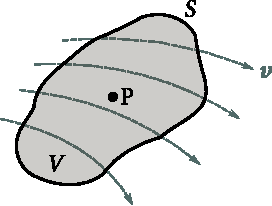
\includegraphics[scale=0.92]{figures/fig_1_23.pdf}
			\caption[]{}
			\label{fig:1_23}
		\end{center}
	\end{minipage}
	\hfill{ }%\hspace{-0.1cm}
	\begin{minipage}[t]{0.5\linewidth}
		\begin{center}
			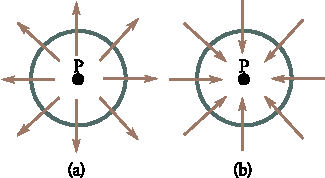
\includegraphics[scale=0.9]{figures/fig_1_24.pdf}
			\caption[]{}
			\label{fig:1_24}
		\end{center}
	\end{minipage}
\vspace{-0.7cm}
\end{figure}

Inspection of \fig{1_23} shows that the distance $\Delta s$, generally speaking, differs in value from the magnitude of the displacement $|\Delta\vec{r}|$. If we take increments of the distance $\Delta s$ and the displacement $\Delta\vec{r}$ corresponding to smaller and smaller time intervals $\Delta t$, then the difference between $\Delta s$ and $|\Delta\vec{r}|$ will diminish, and their ratio in the limit will become equal to unity:
\begin{equation*}
\lim_{\Delta t\to 0} \frac{\Delta s}{|\Delta\vec{r}|} = 1. 
\end{equation*}

\noindent
On these grounds, we can substitute $\Delta s$ for $|\Delta\vec{r}|$ in equation~\eqref{eq:1_59}, which gives us the expression
\begin{equation}\label{eq:1_60}
v = \lim_{\Delta t\to 0} \frac{\Delta s}{\Delta t} = \diff{s}{t}. 
\end{equation}

\noindent
Thus, the magnitude of the velocity equals the derivative of the distance with respect to time.

It is evident that the quantity which in everyday life we call the speed is actually the magnitude of the velocity $\vec{v}$. In uniform motion, the magnitude of the velocity remains constant ($v=\text{constant}$), whereas the direction of the vector $\vec{v}$ changes arbitrarily (in particular it may be constant).

In accordance with \eqn{1_57}, the elementary displacement of a particle is
\begin{equation}\label{eq:1_61}
\mathrm{d}\vec{r} = \vec{v}\,\mathrm{d}{t}. 
\end{equation}

\noindent
Sometimes for clarity's sake, we shall denote an elementary displacement by the symbol $\mathrm{d}\vec{s}$, \ie, write \eqn{1_61} in the form
\begin{equation}\label{eq:1_62}
\mathrm{d}\vec{s} = \vec{v}\,\mathrm{d}{t}. 
\end{equation}

The velocity vector, like any other vector, can be represented in the form
\begin{equation}\label{eq:1_63}
\vec{v} = v_x\vecuni{x} + v_y\vecuni{y} + v_z\vecuni{z}
\end{equation}

\noindent
where $v_x, v_y, v_z$ are the projections of the vector $\vec{v}$ onto the coordinate axes. At the same time, the vector $\dot{\vec{r}}$ equal to $\vec{v}$, according to \eqn{1_43}, can be written as follows:
\vspace{-12pt}
\begin{equation}\label{eq:1_64}
\dot{\vec{r}} = \dot{x}\vecuni{x} + \dot{y}\vecuni{y} + \dot{z}\vecuni{z}
\end{equation}

\noindent
It follows from a comparison of Eqs.~\eqref{eq:1_63} and~\eqref{eq:1_64} that
\begin{equation}\label{eq:1_65}
v_x = \dot{x},\quad v_y = \dot{y},\quad v_z = \dot{z}.
\end{equation}

\noindent
Consequently, the projection of the velocity vector onto a coordinate axis equals the time derivative of the relevant coordinate of the moving particle. Taking \eqn{1_10} into account, we get:
\begin{equation}\label{eq:1_66}
v = \sqrt{\dot{x}^2 + \dot{y}^2 + \dot{z}^2}.
\end{equation}

The velocity vector can be written in the form $\vec{v}=v\vecuni{v}$, where $v$ is the magnitude of the velocity, and $\vecuni{v}$ is the unit vector of $\vec{v}$. Let us introduce the unit vector $\hatvec{\tau}$ of the tangent to a trajectory with its sense the same as that of $\vec{v}$. Hence, obviously, the unit vectors $\vecuni{v}$ and $\hatvec{\tau}$ will coincide, and we can write the following expression:
\vspace{-12pt}
\begin{equation}\label{eq:1_67}
\vec{v} = v\vecuni{v} = v\hatvec{\tau}.
\end{equation}

Let us obtain still another expression for $\vec{v}$. For this purpose, we shall introduce the position vector in the form of $\vec{r}=r\vecuni{r}$ into \eqn{1_57}. According to \eqn{1_49}, we have
\begin{equation}\label{eq:1_68}
\vec{v} = \dot{\vec{r}} = \dot{r}\vecuni{r} + r\dot{\hat{\boldsymbol{e}}}_r.
\end{equation}

\noindent
We shall limit ourselves, for simplicity, to the case when the trajectory is a plane curve, \ie, a curve such that all its points are in a single plane. Let this plane be the plane $x, y$. In \eqn{1_68}, the vector $\vec{v}$ written in the form of two components (\fig{1_25}). The first of them, which we shall designate $\vec{v}_r$, is
\begin{equation}\label{eq:1_69}
\vec{v}_r = \dot{r}\vecuni{r}.
\end{equation}

\noindent
It is directed along the position vector $\vec{r}$ and characterizes the rate of change of the magnitude of $\vec{r}$. The second component, which we shall designate $\vec{v}_{\varphi}$, is
\begin{equation}\label{eq:1_70}
\vec{v}_{\varphi} = r\dot{\hat{\boldsymbol{e}}}_r.
\end{equation}

\noindent
It characterizes the rate of change of the direction of the position vector. 

\begin{figure}[t]
	\begin{center}
		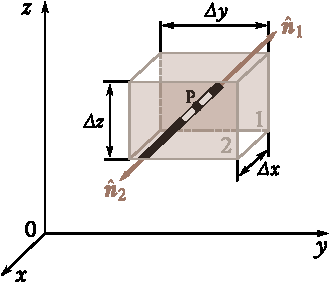
\includegraphics[scale=1]{figures/fig_1_25.pdf}
		\caption[]{}
		\label{fig:1_25}
	\end{center}
	\vspace{-0.7cm}
\end{figure}

Using \eqn{1_56}, we can write that
\begin{equation*}
\dot{\hat{\boldsymbol{e}}}_r = \diff{\varphi}{t}\vecuni{\varphi} = \dot{\varphi}\vecuni{\varphi}
\end{equation*}

\noindent
where $\varphi$ is the angle between the position vector and the $x$-axis, and $\vecuni{\varphi}$ is a unit vector perpendicular to the position vector with its sense in the direction of growth of the angle $\varphi$ [in \eqn{1_56} the symbol $\vecuni{\perp}$ was used for this unit vector]. Using this value in \eqn{1_70}, we get:
\begin{equation}\label{eq:1_71}
\vec{v}_{\varphi} = r\dot{\varphi}\vecuni{\varphi}.
\end{equation}

\noindent
We have introduced the symbols $\vec{v}_{\varphi}$ and $\vecuni{\varphi}$ to underline the fact that the component $\vec{v}_{\varphi}$ and the corresponding unit vector are related to a change in the angle $\varphi$.

The vectors $\vec{v}_r$ and $\vec{v}_{\varphi}$ are obviously mutually perpendicular. Hence,
\begin{equation}\label{eq:1_72}
v = \sqrt{v_r^2 + v_{\varphi}^2} = \sqrt{\dot{r}^2 + r^2\dot{\varphi}^2}.
\end{equation}

Now let us consider how to calculate the distance travelled by a particle from the moment of time $t_1$ to $t_2$ if we know the speed at each moment. Let us divide the interval $t_2-t_1$ into $N$ small, but not necessarily equal intervals: $\Delta t_1$, $\Delta t_2$, \ldots, $\Delta t_N$. The total distance $s$ travelled by a particle can be represented as the sum of the distances $\Delta s_1$, $\Delta s_2$, \ldots, $\Delta s_N$ travelled during the relevant time intervals $\Delta t$:
\begin{equation*}
s = \Delta s_1 + \Delta s_2 + \ldots + \Delta s_N = \sum_{i=1}^{N} \Delta s_i.
\end{equation*}

\noindent
In accordance with \eqn{1_60}, each of the addends can approximately be represented in the form
\begin{equation*}
\Delta s_i \approx v_i \Delta t_i
\end{equation*}

\noindent
where $\Delta t_i$ is the time interval during which the distance $\Delta s_i$ was travelled, and $v_i$ is one of the values of the speed during the time $\Delta t_i$. Hence,
\begin{equation}\label{eq:1_73}
s \approx \sum_{i=1}^{N} v_i \Delta t_i.
\end{equation}

\noindent
This expression will be obeyed more accurately with diminishing time intervals $\Delta t_i$. In the limit when all the $\Delta t_i$'s tend to zero (the number of intervals $\Delta t_i$ will correspondingly grow unlimitedly), the approximate equation will become accurate:
\begin{equation*}
s = \lim_{\Delta t_i\to 0} \sum_{i=1}^{N} v_i \Delta t_i.
\end{equation*}

This expression is a definite integral of the function $v(t)$ taken within the limits from $t_1$ to $t_2$. Thus, the distance travelled by a particle during the interval from $t_1$ to $t_2$ is
\begin{equation}\label{eq:1_74}
s = \int_{t_1}^{t_2} v(t)\,\mathrm{d}t.
\end{equation}

\noindent
It must be underlined that here we are speaking of the speed. If we take an integral of the velocity $\vec{v}(t)$, we get the vector of the displacement of the particle from the point where it was at the moment $t_1$ to the point where it was at the moment $t_2$:
\begin{equation}\label{eq:1_75}
\int_{t_1}^{t_2} v(t)\,\mathrm{d}t = \int_{t_1}^{t_2} \mathrm{d}\vec{r} = \vec{r}_{12}
\end{equation}

\noindent
[see \eqn{1_61}].

If we plot the dependence of $v$ on $t$ (\fig{1_26}), then the distance travelled can be represented as the area of the figure confined between the curve $v(t)$, the straight lines $t = t_1$ and $t = t_2$, and the $t$-axis. Indeed, the product $v_i\Delta t_i$ numerically equals the area of the $i$-th strip. The sum \eqn{1_73} equals the area of the figure confined on top by the broken line formed by the top edges of all such strips. When all the $\Delta t_i$'s tend to zero, the width of a strip diminishes (their number grows simultaneously), and the broken line will coincide with the curve $v = v(t)$ in the limit. Thus, the distance travelled during the time from the moment $t_1$ to the moment $t_2$ numerically equals the area confined between the curve of the function $v = v(t)$, the time axis, and the straight lines $t = t_1$ and $t = t_2$. 

\begin{figure}[t]
	\begin{center}
		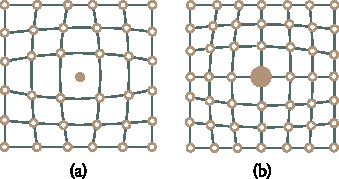
\includegraphics[scale=1]{figures/fig_1_26.pdf}
		\caption[]{}
		\label{fig:1_26}
	\end{center}
	\vspace{-0.8cm}
\end{figure}

It should be noted that the average value of the speed during
the time from $t = t_1$ to $t = t_2$, by definition, is
\begin{equation*}
\average{v} = \frac{s}{t_2-t_1}.
\end{equation*}

\noindent
(The symbol $\langle\rangle$ embracing the $v$ indicates an average.) Introducing into this equation the expression~\eqref{eq:1_74} for $s$, we get
\begin{equation}\label{eq:1_76}
\average{v} = \frac{1}{t_2-t_1}\,\int_{t_1}^{t_2}v(t)\,\mathrm{d}t.
\end{equation}

\noindent
The average values of any scalar or vector functions are calculated in a similar way. For example, the average value of the velocity is
\begin{equation}\label{eq:1_77}
\average{\vec{v}} = \frac{1}{t_2-t_1}\,\int_{t_1}^{t_2}\vec{v}(t)\,\mathrm{d}t = \frac{\vec{r}_{12}}{t_2-t_1}.
\end{equation}

\noindent
[see \eqn{1_75}]. The average value of the function $y(x)$ within the interval from $x_1$ to $x_2$ is determined by the expression
\begin{equation}\label{eq:1_78}
\average{y} = \frac{1}{t_2-t_1}\,\int_{x_1}^{x_2}y(t)\,\mathrm{d}x.
\end{equation}

\section{Acceleration}\label{sec:1_4}

The velocity $\vec{v}$ of a particle can change with time both in magnitude and in direction. The rate of change of the vector $\vec{v}$, like the rate of change of any function of time, is determined by the derivative of the vector $\vec{v}$ with respect to $t$. Denoting this derivative by the symbol $\vec{a}$, we get:
\begin{equation}\label{eq:1_79}
\vec{a} = \lim_{\Delta t\to 0}\frac{\Delta\vec{v}}{\Delta t} = \diff{\vec{v}}{t} = \dot{\vec{v}}.
\end{equation}

\noindent
The quantity determined by equation~\eqref{eq:1_79} is called the \textbf{acceleration} of the particle.

It must be noted that the acceleration $\vec{a}$ plays the same part with respect to $\vec{v}$ as the vector $\vec{v}$ does with respect to the position vector $\vec{r}$.

Equal vectors have identical projections onto the coordinate axes. Consequently, for example,
\begin{equation*}
a_x = \left(\diff{\vec{v}}{t}\right)_{\text{pr. }\vec{x}} = \diff{v_x}{t} = \dot{v}_x
\end{equation*}

\noindent
[see Eqs.~\eqref{eq:1_40}]. At the same time according to Eqs.~\eqref{eq:1_65}, we have $v_x=\dot{x}=\diffin{x}{t}$. Therefore,
\begin{equation*}
\diff{v_x}{t} = \frac{\mathrm{d}}{\mathrm{d}t} \left(\diff{x}{t}\right) = \diffsec{x}{t} = \ddot{x}.
\end{equation*}

\noindent
What we have obtained is that the projection of the acceleration vector onto the $x$-axis equals the second derivative of the coordinate $x$ with respect to time: $a_x=\ddot{x}$. Similar expressions are obtained for the projections of the acceleration onto the $y$- and $z$-axes. Thus,
\begin{equation}\label{eq:1_80}
a_x=\ddot{x},\quad a_y=\ddot{y},\quad a_z=\ddot{z}.
\end{equation}

Using \eqn{1_67} for $\vec{v}$ in~\eqref{eq:1_79}, we get:
\begin{equation}\label{eq:1_81}
\vec{a} = \diff{(v\hatvec{\tau})}{t}.
\end{equation}

\noindent
We remind our reader that $\hatvec{\tau}$ is the unit vector of a tangent to a trajectory having the same direction as $\vec{v}$. According to \eqn{1_49},
\begin{equation}\label{eq:1_82}
\vec{a} = \dot{v}\hatvec{\tau} + v\dot{\hatvec{\tau}}.
\end{equation}

\noindent
Hence, the vector $\vec{a}$ can be represented in the form of the sum of two components. One of them has the direction $\hatvec{\tau}$, \ie, is tangent to the trajectory. It is therefore designated $\vec{a}_{\hatvec{\tau}}$ and is called the \textbf{tangential acceleration}. It equals
\begin{equation}\label{eq:1_83}
\vec{a}_{\hatvec{\tau}} = \dot{v}\hatvec{\tau}.
\end{equation}

\noindent
The second component equal to $v\dot{\hatvec{\tau}}$ is directed, as we shall show below, along a normal to the trajectory. It is therefore designated $\vec{a}_{\hatvec{n}}$ and is called the \textbf{normal acceleration}. Thus,
\begin{equation}\label{eq:1_84}
\vec{a}_{\hatvec{n}} = v\dot{\hatvec{\tau}}.
\end{equation}

In studying the properties of the two components, we shall restrict ourselves for the sake of simplicity to the case when the trajectory is a plane curve.

The magnitude of the tangential acceleration~\eqref{eq:1_83} is
\begin{equation}\label{eq:1_85}
\vec{a}_{\hatvec{\tau}} = |\dot{v}|.
\end{equation}

\noindent
If $\dot{v}>0$ (the velocity grows in magnitude), then the vector $\vec{a}_{\hatvec{\tau}}$ has the same direction as $\hatvec{\tau}$ (\ie, the same direction as $\vec{v}$). If $\dot{v}<0$ (the velocity decreases with time), then the vectors $\vec{v}$ and $\vec{a}_{\hatvec{\tau}}$ have opposite directions. In uniform motion, $\dot{v}=0$, and, therefore, tangential acceleration is absent.

To determine the properties of the normal acceleration [\eqn{1_84}], we must find out what $\dot{\hatvec{\tau}}$, \ie, the rate of change with time of the direction of a tangent to the trajectory, is determined by. It is easy to understand that this rate will grow with an increasing curvature of the trajectory and a higher velocity of a particle along it. 

The degree of bending of a plane curve is characterized by its curvature $C$ determined by the expression
\begin{equation}\label{eq:1_86}
C = \lim_{\Delta t\to 0} \frac{\Delta\varphi}{\Delta s} = \diff{\varphi}{s}
\end{equation}

\noindent
where $\Delta\varphi$ is the angle between tangents to the curve at points spaced $\Delta s$ apart (\fig{1_27}). Thus, the curvature determines the rate of turning of a tangent in motion along a curve.

\begin{figure}[t]
	\begin{center}
		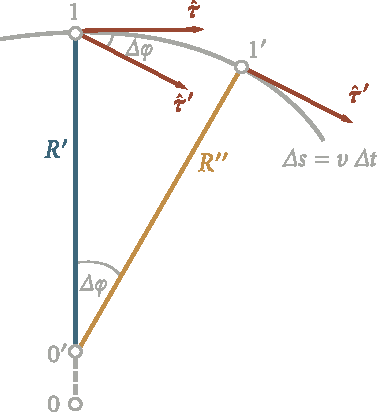
\includegraphics[scale=1]{figures/fig_1_27.pdf}
		\caption[]{}
		\label{fig:1_27}
	\end{center}
	\vspace{-0.7cm}
\end{figure}


The reciprocal of the curvature $C$ is called the \textbf{radius of curvature} at the given point of the curve and is designated $R$:
The degree of bending of a plane curve is characterized by its curvature $C$ determined by the expression
\begin{equation}\label{eq:1_87}
R = \frac{1}{C} = \lim_{\Delta\varphi\to 0} \frac{\Delta s}{\Delta\varphi} = \diff{s}{\varphi}.
\end{equation}

\noindent
The radius of curvature is the radius of a circle that coincides at the given spot with the curve on an infinitely small portion of it. The centre of this circle is defined as the centre of curvature for the given point of the curve.

The radius and centre of curvature at point $1$ (see \fig{1_27}) can be determined as follows. Take point $1'$ near point $1$. Draw the tangents $\hatvec{\tau}$ and $\hatvec{\tau}'$ at these points. The perpendiculars to the tangents will intersect at a certain point $0'$. We must note that for a curve which is not a circle the distances $R'$ and $R''$ will differ somewhat from each other. If point $1'$ is brought closer to point $1$, the point of intersection $0'$ of the perpendiculars will move along the straight line $R'$ and in the limit will be at point $0$. It is exactly the latter that will be the centre of curvature for point $1$. The distances $R'$ and $R"$ will tend to a common limit $R$ equal to the radius of curvature. Indeed, if points $1$ and $1'$ are close to each other, we can write that $\Delta\varphi\approx\Delta s/R'$ or $R' \approx \Delta s/\Delta\varphi$. In the limit when $\Delta\varphi\to 0$, this approximate equation will transform into the strict equation $R=\diffin{s}{\varphi}$ coinciding with the definition of the radius of curvature [see \eqn{1_87}].

Let us now turn to the calculation of an [see \eqn{1_84}]. According to \eqn{1_56},
\begin{equation}\label{eq:1_88}
\dot{\hatvec{\tau}} = \diff{\varphi}{t}\hatvec{n}
\end{equation}

\noindent
where $\hatvec{n}$ is the unit vector of the normal to the trajectory with its sense in the direction of rotation of the vector $\hatvec{\tau}$ when a particle travels along the trajectory [in \eqn{1_56} a similar unit vector was designated $\vecuni{\perp}$]. The quantity $\diffin{\varphi}{t}$ can be related to the radius of curvature of the trajectory and the speed of the particle $\vec{v}$. It follows from \fig{1_27} that
\begin{equation*}
\Delta\varphi\approx \frac{\Delta s}{R'} = \frac{v'\,\Delta t}{R'}
\end{equation*}

\noindent
where $\Delta\varphi$ is the angle of rotation of the vector $\hatvec{\tau}$ during the time $\Delta t$ (coinciding with the angle between the perpendiculars $R'$ and $R''$), and $v'$ is the average speed over the distance $\Delta s$. Hence,
\begin{equation*}
\frac{\Delta\varphi}{\Delta s} \approx \frac{v'}{R'}.
\end{equation*}

\noindent
In the limit when $\Delta t$ tends to zero, the approximate equation will become a strict one, the average speed $v'$ will transform into the instantaneous speed $v$ at point $1$, and $R'$ will become the radius of curvature $R$. As a result, we get the equation
\begin{equation}\label{eq:1_89}
\diff{\varphi}{t} = \frac{v}{R} = vC
\end{equation}

\noindent
($C$ is the curvature). Hence, the rate of rotation of the velocity vector, as we assumed, is proportional to the curvature of the trajectory and the speed of a particle along its trajectory.

Using \eqn{1_89} in~\eqref{eq:1_88}, we find that $\dot{\hatvec{\tau}}=(v/R)\hatvec{n}$. And at last, introducing this expression into \eqn{1_84}, we arrive at the final equation for the normal acceleration:
\vspace{-12pt}
\begin{equation}\label{eq:1_90}
\vec{a}_{\hatvec{n}} = \diff{v^2}{R}\hatvec{n}.
\end{equation}

Thus, the acceleration vector when a particle travels along a plane curve is determined by the following expression:
\begin{equation}\label{eq:1_91}
\vec{a} = \vec{a}_{\hatvec{\tau}} + \vec{a}_{\hatvec{n}} = \dot{v}\hatvec{\tau} + \frac{v^2}{R}\hatvec{n}.
\end{equation}

\noindent
The magnitude of the vector $\vec{a}$ is
\begin{equation}\label{eq:1_92}
a = \sqrt{a_{\hatvec{\tau}}^2 + a_{\hatvec{n}}^2} = \sqrt{\dot{v}^2 + \left(\frac{v^2}{R}\right)^2}.
\end{equation}

In rectilinear motion, the normal acceleration is absent. It must be noted that an vanishes at the inflection point of a curvilinear trajectory (at point IP in \fig{1_28}). At both sides of this point, the vectors $\vec{a}_{\hatvec{n}}$ have different directions. The vector $\vec{a}_{\hatvec{n}}$ cannot change in a jump. Its direction reverses smoothly, and it becomes equal to zero at the inflection point. Assume that a particle is travelling uniformly with an acceleration constant in magnitude. Since in uniform motion the magnitude of the velocity does not change, we have $\vec{a}_{\hatvec{\tau}}=0$, so that $\vec{a}=\vec{a}_{\hatvec{n}}$. The constant magnitude of an signifies that $v^2/R=\text{constant}$. Hence, we conclude that $R=\text{constant}$ ($v=\text{constant}$ because the motion is uniform). This means that the particle is travelling along a curve of constant curvature, \ie, a circle. Thus, when the acceleration of a particle is constant in magnitude and is directed at each moment of time at right angles to the velocity vector, the trajectory of the particle will be a circle.

\begin{figure}[t]
	\begin{center}
		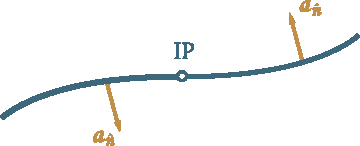
\includegraphics[scale=0.95]{figures/fig_1_28.pdf}
		\caption[]{}
		\label{fig:1_28}
	\end{center}
	\vspace{-0.6cm}
\end{figure}

%\begin{figure}[t]
%	\begin{minipage}[t]{0.5\linewidth}
%		\begin{center}
%			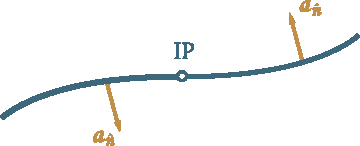
\includegraphics[scale=0.95]{figures/fig_1_28.pdf}
%			\caption[]{}
%			\label{fig:1_28}
%		\end{center}
%	\end{minipage}
%	\hfill{ }%\hspace{-0.1cm}
%	\begin{minipage}[t]{0.5\linewidth}
%		\begin{center}
%			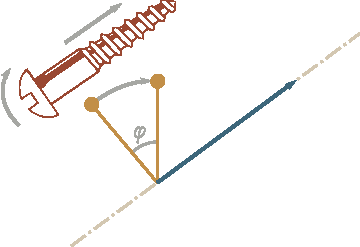
\includegraphics[scale=0.95]{figures/fig_1_29.pdf}
%			\caption[]{}
%			\label{fig:1_29}
%		\end{center}
%	\end{minipage}
%	\vspace{-0.4cm}
%\end{figure}

\section{Circular Motion}\label{sec:1_5}

The rotation of a body through a certain angle $\varphi$ can be given in the form of a straight line whose length is $\varphi$ and whose direction coincides with the axis about which the body is rotating. To indicate the direction of rotation about a given axis, it is related to the line depicting rotation by the \textbf{right-hand screw rule}: the line should be directed so that when looking along it (\fig{1_29}) we see clockwise rotation (when rotating the head of a right-hand screw clockwise, we cause it to move away from us). We showed in Sec.~\ref{sec:1_2} (see \fig{1_4}) that rotations through finite angles are not added by the parallelogram method and are therefore not vectors. Matters are different for rotations through very small angles $\Delta\vec{\varphi}$. The distance travelled by any point of a body when rotated through a very small angle can be considered as a straight line (\fig{1_30}). Consequently, two small circular motions $\Delta\vec{\varphi}_1$ and $\Delta\vec{\varphi}_2$ performed sequentially, as can be seen from the figure, result in the same displacement $\Delta\vec{r}_3=\Delta\vec{r}_1+\Delta\vec{r}_2$ of any point of the body as the circular motion $\Delta\vec{\varphi}_3$ obtained from $\Delta\vec{\varphi}_1$ and $\Delta\vec{\varphi}_2$ by addition using the parallelogram method. Hence it follows that very small circular motions can be considered as vectors (we shall denote these vectors by $\Delta\vec{\varphi}$ or $\mathrm{d}\vec{\varphi}$). The direction of the rotation vector is associated with the direction of rotation of a body. Consequently, $\mathrm{d}\vec{\varphi}$ is not a true vector, but a pseudovector.

\begin{figure}[t]
	\begin{center}
		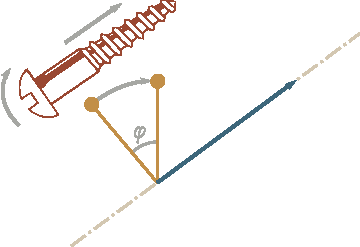
\includegraphics[scale=0.95]{figures/fig_1_29.pdf}
		\caption[]{}
		\label{fig:1_29}
	\end{center}
	\vspace{-0.7cm}
\end{figure}

The vector quantity
\begin{equation}\label{eq:1_93}
\vec{\omega} = \lim_{\Delta t\to 0} \frac{\Delta\vec{\varphi}}{\Delta t} = \diff{\vec{\varphi}}{t}
\end{equation}

\noindent
(where $\Delta t$ is the time during which the circular motion $\Delta\vec{\varphi}$ is performed) is called the angular velocity of a body\footnote{The velocity $\vec{v}$ considered in Sec.~\ref{sec:1_3} is sometimes called linear.}. The angular velocity $\vec{\omega}$ is directed along the axis about which the body is rotating in a direction determined by the right-hand screw rule (\fig{1_31}) and is a pseudovector. The magnitude of the angular velocity, \ie, the angular speed, equals $\diffin{\varphi}{t}$. Circular motion at a constant angular velocity is called uniform. For uniform circular motion, we have $\omega=\varphi t$, where $\varphi$ is the finite angle of rotation during the time $t$ (compare with $v=s/t$). Thus, in uniform circular motion, $\omega$ shows the angle through which a body rotates in unit time.

\begin{figure}[t]
	\begin{minipage}[t]{0.5\linewidth}
		\begin{center}
			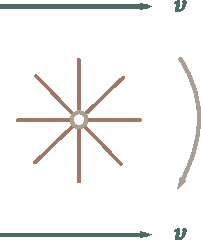
\includegraphics[scale=1]{figures/fig_1_30.pdf}
			\caption[]{}
			\label{fig:1_30}
		\end{center}
	\end{minipage}
	\hspace{-0.1cm}
	\begin{minipage}[t]{0.5\linewidth}
		\begin{center}
			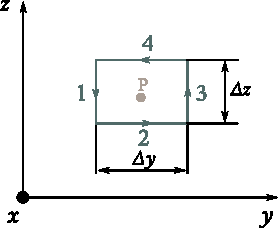
\includegraphics[scale=0.95]{figures/fig_1_31.pdf}
			\caption[]{}
			\label{fig:1_31}
		\end{center}
	\end{minipage}
	\vspace{-0.5cm}
\end{figure}

Uniform circular motion can be characterized by the \textbf{period of revolution} $T$. It is defined as the time  during which a body completes one revolution, i.e. rotates through the angle \SI{2\pi}{\radian}, or \SI{360}{\degree}. Since the time interval $\Delta t=T$ corresponds to the angle of rotation $\Delta\varphi=2\pi$, we have
\begin{equation}\label{eq:1_94}
\omega = \frac{2\pi}{T}
\end{equation}

\noindent
whence
\begin{equation}\label{eq:1_95}
T = \frac{2\pi}{\omega}.
\end{equation}

The number of revolutions in unit time $\nu$ is evidently equal to
\begin{equation}\label{eq:1_96}
\nu = \frac{1}{T} = \frac{\omega}{2\pi}.
\end{equation}

\noindent
It follows from \eqn{1_96} that the angular velocity equals $2\pi$ multiplied by the number of revolutions per unit time:
\begin{equation}\label{eq:1_97}
\omega = 2\pi\nu.
\end{equation}

The concepts of the period of revolution and the number of revolutions per unit time can also be retained for non-uniform circular motion. Here, we must understand the instantaneous value of $T$ to signify the time during which a body would perform one revolution if it rotated uniformly with the given instantaneous value of the angular velocity, and $\nu$ to signify the number of revolutions which a body would complete in unit time in similar conditions.

The vector $\vec{\omega}$ may vary either as a result of a change in the speed of rotation of a body about its axis (in this case it changes in magnitude), or as a result of turning of the axis of rotation in space (in this case $\vec{\omega}$ changes in direction). Assume that during the time $\Delta t$ the vector $\vec{\omega}$ receives the increment $\Delta\vec{\omega}$. The change in the angular velocity vector with time is characterized by the quantity
\begin{equation}\label{eq:1_98}
\vec{\alpha} = \lim_{\Delta t\to 0} \frac{\Delta\vec{\omega}}{t} = \diff{\vec{\omega}}{t}
\end{equation}

\noindent
called the \textbf{angular acceleration}. The latter, like the angular velocity, is a pseudovector.

%\begin{figure}[t]
%	\begin{center}
%		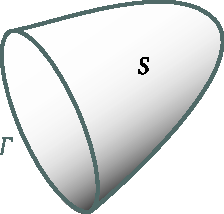
\includegraphics[scale=1]{figures/fig_1_32.pdf}
%		\caption[]{}
%		\label{fig:1_32}
%	\end{center}
%\vspace{-0.7cm}
%\end{figure}
\begin{figure}[t]
	\begin{minipage}[t]{0.5\linewidth}
		\begin{center}
			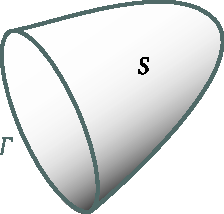
\includegraphics[scale=1]{figures/fig_1_32.pdf}
			\caption[]{}
			\label{fig:1_32}
		\end{center}
	\end{minipage}
	\hspace{-0.1cm}
	\begin{minipage}[t]{0.5\linewidth}
		\begin{center}
			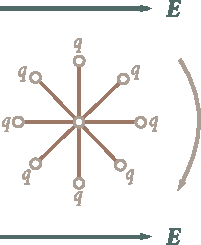
\includegraphics[scale=1]{figures/fig_1_33.pdf}
			\caption[]{}
			\label{fig:1_33}
		\end{center}
	\end{minipage}
	\vspace{-0.6cm}
\end{figure}

Different points of a body in circular motion have different linear velocities $\vec{v}$. The velocity of each point continuously changes its direction. The speed $v$ is determined by the speed of rotation of the body $\omega$ and the distance $R$ to the point being considered from the axis of rotation. Assume that during a small interval of time the body turned through the angle $\Delta\varphi$ (\fig{1_32}). The point at the distance $R$ from the axis travels the path $\Delta s=R\Delta\varphi$. The linear speed of the point is
\begin{equation*}
v = \lim_{\Delta t\to 0} \frac{\Delta s}{\Delta t} = \lim_{\Delta t\to 0} R\frac{\Delta\varphi}{\Delta t} = R \lim_{\Delta t\to 0} \frac{\Delta\varphi}{\Delta t} = R\diff{\varphi}{t} = R\omega.
\end{equation*}

\noindent
Thus,
\begin{equation}\label{eq:1_99}
v = \omega R.
\end{equation}

Equation~\eqref{eq:1_99} relates the linear and the angular speeds. Let us find an expression relating the relevant velocities $\vec{v}$ and $\vec{\omega}$. We shall determine the position of the point of the body being considered by the position vector $\vec{r}$ drawn from the origin of coordinates on the axis of rotation (\fig{1_33}). Examination of the figure shows that the vector product $\vecprod{\omega}{r}$ coincides in direction with the vector $\vec{v}$ and its magnitude is $\omega r\sin\alpha=\omega R$. Hence,
\begin{equation}\label{eq:1_100}
\vec{v} = \vecprod{\omega}{r}.
\end{equation}

%\begin{figure}[t]
%	\begin{center}
%		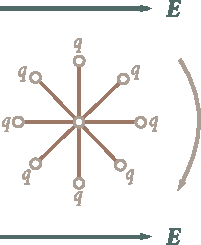
\includegraphics[scale=1]{figures/fig_1_33.pdf}
%		\caption[]{}
%		\label{fig:1_33}
%	\end{center}
%	\vspace{-0.7cm}
%\end{figure}

The normal acceleration of the points of a rotating body is $\vec{a}_{\hatvec{n}}=v^2/R$. Introducing into this expression the value of $v$ from \eqn{1_99}, we get
\begin{equation}\label{eq:1_101}
a_{\hatvec{n}} = \omega^2 R.
\end{equation}

\noindent
If we introduce the vector $\vec{R}$ drawn to the given point of the body from the axis of rotation at right angles to the latter (see \fig{1_33}), then \eqn{1_101} can be given a vector form:
\begin{equation}\label{eq:1_102}
\vec{a}_{\hatvec{n}} = -\omega^2 \vec{R}.
\end{equation}

\noindent
There is a minus sign in this formula because the vectors $\vec{a}_{\hatvec{n}}$ and $\vec{R}$ have opposite directions.

Let us assume that the axis of rotation of a body does not turn in space. According to \eqn{1_85}, the magnitude of the tangential acceleration is $|\diffin{v}{t}|$. Using equation~\eqref{eq:1_99} and taking into account that the distance to the point being considered from the axis of rotation $R=\text{constant}$, we can write
\begin{equation*}
a_{\hatvec{\tau}} = \left| \lim_{\Delta t\to 0} \frac{\Delta v}{\Delta t} \right| = \left| \lim_{\Delta t\to 0} \frac{\Delta(\omega R)}{\Delta t} \right| = R \left| \lim_{\Delta t\to 0} \frac{\Delta(\omega)}{\Delta t} \right| = R\alpha
\end{equation*}

\noindent
where $\alpha$, is the magnitude of the angular acceleration. Consequently, the magnitude of the tangential acceleration is related to the magnitude of the angular acceleration as follows:
\begin{equation}\label{eq:1_103}
a_{\hatvec{\tau}} = \alpha R.
\end{equation}

Thus, the normal and tangential accelerations grow linearly with an increasing distance to a point from the axis of rotation.

\cleardoublepage
% !TEX root = saveliev_physics_general_course_1.tex
%!TEX TS-program = pdflatex
%!TEX encoding = UTF-8 Unicode


\chapter{DYNAMICS OF A POINT PARTICLE}\label{chap:2}

\section{Classical Mechanics. Range of Its Applicability}\label{sec:2_1}

Kinematics describes the motion of bodies without being concerned with why a body moves exactly in a given way (for example, uniformly along a circle, or with uniform acceleration along a straight line), and not in a different one. 

Dynamics studies the motion of bodies in connection with its causes (the interactions between bodies) resulting in the occurrence of a specific kind of motion.

The so-called classical or Newtonian mechanics is based on three laws of dynamics that were formulated by Isaac Newton in 1687.

Newton's laws (like all other laws of physics) were the result of generalizing a great amount of experimental facts. Their correctness (although it covers a very extensive range of phenomena, the latter are nevertheless limited) is confirmed by the agreement of the corollaries following from them with experimental results.

Newtonian mechanics achieved such great successes during two centuries that many physicists of the 19th century were convinced in its omnipotence. It was considered that the explanation of any physical phenomenon required its reduction to a mechanical process obeying Newton's laws. With the development of science, however, new facts were uncovered for which no place could be found within the confines of classical mechanics. These facts were explained in new theories---the special theory of relativity and quantum mechanics.

The special theory of relativity advanced by Albert Einstein in 1905 radically revised Newton's notions of space and time. This revision resulted in the creation of ``high-speed mechanics'' or, as it is called, relativistic mechanics. The new mechanics did not result, however, in complete negation of the old Newtonian mechanics. The equations of relativistic mechanics in their limit (for speeds small in comparison with the speed of light) transform into the equations of classical mechanics. Thus, classical mechanics has entered relativistic mechanics as a particular case of it and has retained its previous significance for describing motions occurring at speeds much smaller than that of light.

Matters are similar with the relation between classical and quantum mechanics. The latter took root in the twenties of the present century as a result of the development of physics of the atom. The equations of quantum mechanics also result in those of classical mechanics in their limit (for masses that are great in comparison with the masses of atoms). Consequently, classical mechanics is also a part of quantum mechanics and is a limiting case of it.

Thus, the development of science has not eliminated classical mechanics, but has only shown its limited applicability. Classical mechanics based on Newton's laws is the mechanics for bodies of large (compared with the mass of atoms) masses travelling at low (compared with the speed of light) speeds.

\section{Newton's First Law. Inertial Reference Frames}\label{sec:2_2}

Newton's first law is formulated as follows: \textit{every body continues in its state of rest or of uniform motion in a straight line unless it is compelled by external forces to change that state}. Both states named are distinguished by the acceleration of the body equalling zero. Therefore, the first law can also be formulated as follows: the velocity of every body remains constant (in particular, it equals zero) until the action of other bodies on this body causes it to change.

Newton's first law is obeyed not in any reference frame. We have already noted that the nature of motion depends on the choice of the reference frame. Let us consider two frames of reference moving with respect to each other with a certain acceleration. If a body is at rest relative to one of them, then it will obviously travel with acceleration relative to the other one. Consequently, Newton's first law cannot be obeyed simultaneously in both frames.

A reference frame in which Newton's first law is obeyed is called an \textbf{inertial} one. The law itself is quite often called the \textbf{law of inertia}. A reference frame in which Newton's first law is not obeyed is called a non-inertial reference frame. There is an infinite multitude of inertial frames. Any reference frame moving uniformly in a straight line (\ie, with a constant velocity) relative to an inertial frame will also be an inertial one. This will be discussed in greater detail in Sec.~\ref{sec:2_7}.

It has been established experimentally that the reference frame whose centre coincides with the Sun and whose axes are directed toward appropriately selected stars is an inertial one. This system is defined as a \textbf{heliocentric reference frame} (\textit{helios} means Sun in Greek). Any reference frame moving uniformly in a straight line relative to the heliocentric frame will be an inertial one.

The Earth moves relative to the Sun and stars along a curvilinear trajectory having the shape of an ellipse. Curvilinear motion always occurs with a certain acceleration. The Earth also rotates about its axis. For these reasons, a reference frame associated with the Earth's surface travels with acceleration relative to the heliocentric reference frame, and is not inertial. The acceleration of such a frame, however, is so small that it may be considered practically inertial in a great number of cases. But sometimes the non-inertial nature of a reference frame associated with the Earth significantly affect the nature of mechanical phenomena being considered relative to it. We shall treat some of these cases on a later page.

\section{Mass and Momentum of a Body}\label{sec:2_3}

The action of other bodies on a given one causes its velocity to change, \ie, imparts an acceleration to it. Experiments show that the same action imparts accelerations differing in magnitude to different bodies. Every body resists attempts to change its state of motion. This property of bodies is called \textbf{inertia}. It is characterized quantitatively by a physical quantity called the \textbf{mass} of a body.

To find the mass of a body, we must compare it with that of the body taken as the standard of mass. We can also compare the mass of the given body with that of a body having a known mass (found by comparing it with the standard). The masses $m_1$ and $m_2$ of two point particles can be compared as follows. We place the particles in conditions allowing us to ignore their interaction with other bodies. A system of bodies interacting only with one another and not interacting with other bodies is called \textbf{isolated}. We are therefore considering an isolated system of two particles. If we make these particles interact (for example, by colliding with each other), their velocities receive the increments $\Delta\vec{v}_1$ and $\Delta\vec{v}_2$. Experiments show that these increments are always directed oppositely, \ie, differ in their sign. The ratio of the magnitudes of the velocity increments, however, does not depend on the method and intensity of interaction of the given two bodies or particles\footnote{This holds for the case when the initial and final velocities of the particles are small in comparison with the speed of light $c$.}. This ratio is inversely proportional to the ratio of the masses of the bodies being considered:
\vspace{-10pt}
\begin{equation}\label{eq:2_1}
\frac{|\Delta\vec{v}_1|}{\Delta\vec{v}_2} = \frac{m_2}{m_1}
\end{equation}

\noindent
(the velocity of the body with the greater inertia, \ie, with the larger mass, changes less). Taking into account the relative direction of the vectors $\Delta\vec{v}_1$ and $\Delta\vec{v}_2$,~\eqn{2_1} can be written in the form
\begin{equation}\label{eq:2_2}
m_1 \Delta\vec{v}_1 = - m_2 \Delta\vec{v}_2.
\end{equation}

In Newtonian mechanics (\ie, in mechanics based on Newton's laws), the mass of a body is assumed to be a constant quantity not depending on its velocity. At velocities smaller than the speed of light $c$ (when $v\ll c$), this assumption is obeyed in practice. Taking advantage of the constancy of mass, we can write~\eqn{2_2} as follows:
\begin{equation}\label{eq:2_3}
\Delta(m_1 \vec{v}_1) = - \Delta(m_2 \vec{v}_2).
\end{equation}

The product of the mass and the velocity of a body is called its \textbf{momentum}. Using the symbol $\vec{p}$ for it, we get
\begin{equation}\label{eq:2_4}
\vec{p} = m \vec{v}.
\end{equation}

\noindent
Definition~\eqref{eq:2_4} holds for point particles and extended bodies in translational motion. When we have to do with an extended body whose motion is not translational, we must imagine the body as a combination of particles of masses $\Delta m_i$, determine the momenta $\Delta m_i\vec{v}_i$ of these particles, and then add these momenta vectorially. The result will be the total momentum of the body:
\begin{equation}\label{eq:2_5}
\vec{p} = \sum_{i} m_i \vec{v}_i.
\end{equation}

\noindent
In translation of a body, all the $\vec{v}_i$'s are the same, and~\eqn{2_5} transforms into~\eqref{eq:2_4}. 

Substituting the momenta $\vec{p}$ for the products $m\vec{v}$ in~\eqn{2_3}, we get $\Delta\vec{p}_1=\Delta\vec{p}_2$, whence $\Delta(\vec{p}_1+\vec{p}_2)=0$. When the increment of a quantity equals zero, this signifies that the quantity itself remains unchanged. We have thus arrived at the conclusion that \textit{the total momentum of an isolated system of two interacting particles remains constant}:
\begin{equation}\label{eq:2_6}
\vec{p} = \vec{p}_1 + \vec{p}_2 = \text{constant}.
\end{equation}

\noindent
The above statement forms the \textbf{law of conservation of momentum}. We shall consider this law in greater detail in Sec.~\ref{sec:3_10}.

We must note here that in relativistic mechanics (see Chap. ~\ref{chap:8}) the expression for the momentum is more complicated than~\eqn{2_4}:
\begin{equation}\label{eq:2_7}
\vec{p} = \frac{m \vec{v}}{\sqrt{1 - v^2/c^2}}.
\end{equation}

\noindent
Here $m$ is the so-called \textbf{rest mass} of a body (its mass at $v=0$), and $c$ is the speed of light in a vacuum. Equation~\eqref{eq:2_7} can be interpreted to state that the mass of a body does not remain constant (as is assumed in Newtonian mechanics), but changes with the speed according to the law
\begin{equation}\label{eq:2_8}
m(v) = \frac{m}{\sqrt{1 - v^2/c^2}}
\end{equation}

\noindent
Hence, \eqn{2_7} can be written as follows:
\begin{equation}\label{eq:2_9}
\vec{p} = m(v)\,\vec{v}
\end{equation}

\noindent
\ie, in a form similar to~\eqn{2_4}.

The mass $m(v)$ determined by~\eqn{2_8} is called the \textbf{relativistic mass}. We shall designate it by the symbol $\mr$ in the following.

\section{Newton's Second Law}\label{sec:2_4}

Newton's second law states that \textit{the rate of change of the momentum of a body equals the force $\vec{F}$ acting on the body}:
\begin{equation}\label{eq:2_10}
\diff{\vec{p}}{t} = \vec{F}.
\end{equation}

\noindent
Equation~\eqref{eq:2_10} is called the \textbf{equation of motion of a body}.

Substituting $m\vec{v}$ for $\vec{p}$ according to~\eqn{2_4} and taking into account that in Newtonian mechanics the mass is assumed to be constant, we can write~\eqn{2_10} in the form
\begin{equation}\label{eq:2_11}
m\vec{a} = \vec{F}
\end{equation}

\noindent
where $\vec{a}=\dot{\vec{v}}$. We have thus arrived at a different formulation of Newton's second law: \textit{the product of the mass of a body and its acceleration equals the force acting on the body}.

Equation~\eqref{eq:2_11} has called forth and is continuing to call forth many controversies among physicists. To date, there is no generally adopted interpretation of this relation. The complication consists in that there are no independent ways of determining the quantities $m$ and $\vec{F}$ in~\eqn{2_11}. To determine one of them ($m$ or $\vec{F}$), we have to use~\eqn{2_11} relating it to the other one and to the acceleration $\vec{a}$. For example, according to S. Khaikin\footnote{S. E. Khaikin. Fizicheskie osnovy mekhaniki (The Physical Fundamentals of Mechanics). Moscow, Fizmatgiz (1963), p. 104.}, ``Since to establish a way of measuring the mass of a body we use the same second law of Newton (the magnitude of the mass of a body is determined by simultaneously measuring the force and the acceleration), then Newton's second law contains, on the one hand, a statement that the acceleration is proportional to the force, and on the other, a definition of the mass of a body as the ratio of the force acting on it to the acceleration imparted to this body''.

R. Feynman states the following about the meaning of Newton's second law: ``Let us ask, `What is the meaning of the physical laws of Newton, which we write as $F=ma$? What is the meaning of force, mass, and acceleration?' Well, we can intuitively sense the meaning of mass, and we can define acceleration if we know the meaning of position and time. We shall not discuss these meanings, but shall concentrate on the new concept of force. The answer is equally simple: `If a body is accelerating, then there is a force on it'. That is what Newton's laws say, so the most precise and beautiful definition of force imaginable might simply be to say that force is the mass of an object times the acceleration\ldots''. However, ``if we have discovered a fundamental law, which asserts that the force is equal to the mass times the acceleration, and then \textit{define} the force to be the mass times the acceleration, we have found out nothing\ldots, such things certainly cannot be the content of physics, because they are definitions going in a circle\ldots no prediction whatsoever can be made from a definition\ldots. The real content of Newton's laws is this: that the force is supposed to have some independent properties, in addition to the law $\vec{F}=m\vec{a}$; but the specific independent properties that the force has were not completely described by Newton or by anybody else\ldots''\footnote{R. P. Feynman, R. B. Leighton, M. Sands. The Feynman Lectures on Physics. Reading, Mass., Addison-Wesley (1965), p. 12-1.}.

We must underline the fact that Newton's second law (like his other two laws) is an experimental one. It took shape as a result of generalization of the data of experiments and observations.

In a particular case when $\vec{F}=0$ (\ie, in the absence of action on a body by other bodies), the acceleration, as follows from~\eqn{2_11}, also equals zero. This conclusion coincides with Newton's first law. Therefore, the first law is contained in the second one as a particular case of it. Notwithstanding this circumstance, the first law is formulated independently of the second one because it contains in essence the postulate (statement) of the existence of inertial reference frames.

In conclusion, we shall note that upon an independent choice of the units of mass, force, and acceleration, the second law must be written in the form
\begin{equation}\label{eq:2_12}
m\vec{a} = k\vec{F}
\end{equation}

\noindent
where $k$ is a constant of proportionality.

\section{Units and Dimensions of Physical Quantities}\label{sec:2_5}

The laws of physics, as we have already noted, establish quantitative relations between physical quantities. To establish such relations, it is necessary to be able to measure various physical quantities.

To measure a physical quantity (for example, speed) means to compare it with a quantity of the same kind (in our example with speed) taken as a unit.

Generally speaking, we could establish a unit for every physical quantity arbitrarily, regardless of other quantities. We can limit ourselves, however, to an arbitrary choice of the units for only a few (at least three) quantities taken as the basic ones. Any quantities can be taken as the basic ones in principle. The units of all other quantities can be established with the aid of these basic units using for this purpose the physical laws relating the relevant quantity to the basic ones or to quantities for which the units have already been established in this way.

Let us consider the following example to explain what has been said above. Assume that we have already established the units for mass and acceleration. Equation~\eqref{eq:2_12} expresses the law relating these quantities to a third physical quantity ---force. We choose the unit of force so that the proportionality constant in this equation will equal unity. Equation~\eqref{eq:2_12} thus acquires a simple form:
\begin{equation}\label{eq:2_13}
m\vec{a} = \vec{F}.
\end{equation}

\noindent
It follows from~\eqn{2_13} that the established unit of force is a force such that a body of unit mass receives an acceleration of unity under its action [substitution of $F=1$ and $m=1$ in~\eqn{2_13} gives $a=1$].

When units are selected in this way, physical relations acquire a simpler form. The combination of units themselves forms a definite system.

There are several systems differing in the selection of the basic units. Systems based on the units of length, mass, and time are called \textbf{absolute}.

USSR State Standard GOST 9867-61 in force from January 1, 1963, provides for the use of the International System of Units, designated SI, in the USSR. This system of units has been introduced as preferable in all fields of science, engineering, and the national economy, and also in education. The basic units of the SI system include the unit of length---the metre (its symbol is \si{\metre}), the unit of mass---the kilogramme (\si{\kilo\gram}), and the unit of time---the second (\si{\second}). The SI system is thus an absolute one. In addition to the three units indicated above, the other basic units of this system are the unit of current---the ampere (\si{\ampere}), the unit of thermodynamic temperature---the kelvin (\si{\kelvin}), the unit of luminous intensity---the candela (\si{\candela}), and the unit of the amount of substance---the mole (\si{\mole}). These units will be treated in the corresponding parts of our course.

The metre is defined as the length equal to $1,650,763.73$ wavelengths in vacuum of the radiation corresponding to the transition between the levels \enlevel{2}{p}{10} and \enlevel{5}{d}{5} of the krypton-86 atom\footnote{The meaning of these symbols will be explained in Vol. III in the part ``Atomic Physics''.} (the orange line of krypton-86). The metre approximately equals $1/40,000,000$th of the length of an Earth's meridian. Multiple and submultiple units are also used, namely, the kilometre ($\SI{1}{\kilo\metre}=\SI{103}{\metre}$), the centimetre ($\SI{1}{\centi\metre}=\SI{e-2}{\metre}$), the millimetre ($\SI{1}{\milli\metre}=\SI{e-3}{\metre}$), the micrometre ($\SI{1}{\micro\metre}=\SI{e-6}{\metre}$), etc.

The kilogramme is the mass of a platinum and iridium\footnote{An alloy of platinum and iridium has a high hardness and resistance to corrosion (\ie, is virtually not subjected to the chemical action of the surroundings).} body kept in the International Chamber of Weights and Measures at S\`evre (near Paris). This body is called the international prototype of the kilogramme. The mass of this prototype is close to that of \SI{1000}{\cubed\centi\metre} of pure water at \SI{4}{\degreeCelsius}. A gramme equals one-thousandth of a kilogramme.

The second is the duration of $9,192,631,770$ periods of the radiation corresponding to the transition between the two hyperfine levels of the ground state of the cesium-133 atom. The second approximately equals $1/86,400$ of the mean solar day.

Physics also employs an absolute system of units called the cgs system. The basic units in this system are the centimetre, gramme, and second.

The units of the quantities that we introduced in kinematics (velocity and acceleration) are derived from the basic units. Thus, the unit of velocity (or speed) is the velocity of a body in uniform motion that travels a distance of unit length (metre or centimetre) in unit time (second). This unit is designated \si{\metre\per\second} in the SI system and \si{\centi\metre\per\second} in the cgs system. The unit of acceleration is the acceleration of uniformly varying motion when the velocity of a body changes by one unit (one \si{\metre\per\second} or \si{\centi\metre\per\second}) in unit time (\si{\second}). This unit is designated \si{\metre\per\square\second} in the SI system and \si{\centi\metre\per\square\second} in the cgs system.

The unit of force in the SI system is called the newton (\si{\newton}). According to~\eqn{2_13}, one newton equals the force that imparts an acceleration of \SI{1}{\metre\per\square\second} to a body with a mass of \SI{1}{\kilo\gram}. The unit of force in the cgs system is called the dyne (\si{\dyne}). One dyne equals the force that imparts an acceleration of \SI{1}{\centi\metre\per\square\second} to a body with a mass of \SI{1}{\gram}. The newton and dyne are related as follows:
\begin{equation*}
\SI{1}{\newton} = \SI{1}{\kilo\gram} \times \SI{1}{\metre\square\second} = \SI{e3}{\gram} \times \SI{e2}{\centi\metre\square\second}
\end{equation*}

The mk(force)s system (usually called the technical system) is widely used in engineering. The basic units of this system are the metre, the unit of force---the kilogramme-force (\si{\kgf}), and the second. The kilogramme-force is defined as the force that imparts an acceleration of $\SI{9.80655}{\metre\per\second}$ (the normal acceleration of free fall) to a mass of \SI{1}{\kilo\gram}. It follows from this definition that $\SI{1}{\kgf}=\SI{9.80655}{\newton}$ (approximately \SI{9.81}{\newton}).

The unit of mass in the mk(force)s system, according to~\eqn{2_13}, should be taken equal to the mass of a body that receives an acceleration of \SI{1}{\metre\per\square\second} when acted upon by a force of \SI{1}{\kgf}. Although many names have been proposed for this unit\footnote{See L. A. Sena. Units of Physical Quantities and Their Dimensions. 2nd ed., Moscow, Mir Publishers (1975), pp. 9, 54}, none of them has been legalized, and it is designated \si{\kgf\second\squared\per\metre}. It is obvious that $\SI{1}{\kgf\second\squared\per\metre}=\SI{9.80655}{\kilo\gram}$ (approximately \SI{9.81}{\kilo\gram}).

It follows from the way a system of units is constructed that a change in the basic units leads to a change in the derived ones. If, for example, the minute is taken as the unit of time instead of the second, \ie, the unit of time is increased $60$ times, then the unit of velocity will diminish $60$ times, and the unit of acceleration will diminish $3600$ times.

The relation showing how a unit of a quantity changes when the basic units are changed is called the dimension of this quantity. The dimension of an arbitrary physical quantity is designated by its symbol placed in brackets. For example, $[v]$ stands for the dimension of velocity. Special symbols are used for the dimensions of the basic quantities: L for the length, M for the mass, and T for the time. Thus, designating the length by $l$, the mass by $m$, and the time by $t$, we can write
\begin{equation*}
[l] = \text{L},\quad [m] = \text{M},\quad [t] = \text{T}.
\end{equation*}

When these symbols are used, the dimension of an arbitrary physical quantity has the form L$^{\alpha}$M$^{\beta}$T$^{\gamma}$ ($\alpha$, $\beta$ and $\gamma$ may be either positive or negative, and in particular may equal zero). This notation signifies that when the unit of length is increased $n_1$ times, the unit of a given quantity grows $n_1^{\alpha}$ times (accordingly, the number that expresses the value of the quantity in these units diminishes $n_1^{\alpha}$ times). When the unit of mass is increased $n_2$ times, the unit of the given quantity grows $n_2^{\beta}$ times. Finally, when the unit of time is increased $n_3$ times, the unit of the given quantity grows $n_3^{\gamma}$ times.

Since physical laws cannot depend on the selection of the units for the quantities figuring in them, the dimensions of both sides of the equations expressing these laws must be the same. This condition can be used, first, for verifying the correctness of physical relations obtained, and, second, for establishing the dimensions of physical quantities. For example, speed is determined by the formula $v = \Delta s/\Delta t$. The dimension of $\Delta s$ is L, and that of $\Delta t$ is T. The dimension of the right-hand side of the above formula is $[\Delta s]/[\Delta t]=\text{L/T}=\text{LT}^{-1}$. The dimension of the left-hand side must be the same. Hence,
\begin{equation}\label{eq:2_14}
[v] = \text{LT}^{-1}.
\end{equation}

\noindent
This relation is called a dimension formula, and its right-hand side the dimension of the relevant quantity (in our case, of speed).

The relation $a = \Delta v/\Delta t$ permits us to establish the dimension of acceleration:
\begin{equation}\label{eq:2_15}
[a] = \frac{[\Delta v]}{[\Delta t]} = \frac{\text{LT}^{-1}}{\text{T}} = \text{LT}^{-2}.
\end{equation}

\noindent
The dimension of force is
\begin{equation}\label{eq:2_16}
[F] = [m][a] = \text{MLT}^{-2}.
\end{equation}

\noindent
The dimensions of all other quantities are established in a similar way.

\section{Newton's Third Law}\label{sec:2_6}

\begin{figure}[t]
	\begin{center}
		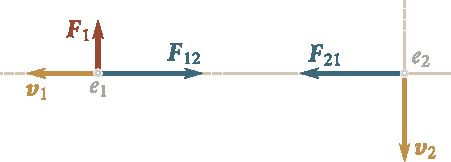
\includegraphics[scale=1]{figures/cap_02/fig_2_1.pdf}
		\caption[]{}
		\label{fig:2_1}
	\end{center}
	\vspace{-0.7cm}
\end{figure}

Any action of bodies on one another has the nature of mutual interaction: if body $1$ acts on body $2$ with the force $\vec{F}_{21}$ then body 2, in turn, acts on body $1$ with the force $\vec{F}_{12}$.

Newton's third law states that \textit{the forces exerted by interacting bodies on each other are equal in magnitude and opposite in direction}. Using the above symbols for such forces, the third law can be expressed in the form of the equation
\begin{equation}\label{eq:2_17}
\vec{F}_{12} = - \vec{F}_{21}.
\end{equation}

It follows from Newton's third law that forces appear in pairs: for any force applied to a body there is another force equal in magnitude and opposite in direction applied to the second body interacting with the first one.

Newton's third law is not always correct. It is observed quite strictly in contact interactions (\ie, interactions observed upon the direct contact of bodies), and also when bodies at rest that are a certain distance apart interact with each other.

As an example of the violation of Newton's third law, we can take a system of two charged particles $e_1$ and $e_2$ moving at the given moment as shown in~\fig{2_1}. It is proved in electrodynamics that apart from the force of electrostatic interaction $\vec{F}_{12}$ obeying the third law, the magnetic force $\vec{F}_1$ will also be exerted on the first particle. Only the force $\vec{F}_{21}$ equal to $-\vec{F}_{12}$ acts on the second particle. The magnitude of the magnetic force acting on the second particle for the case shown in the figure equals zero. It must be noted that for speeds of particles that are much smaller than the speed of light in a vacuum (when $v_1\ll c$ and $v_2\ll c$) the force $\vec{F}_1$ is negligibly small in comparison with the force $\vec{F}_{12}$, so that Newton's third law is virtually correct in this case too.

Now let us consider a system of two electrically neutral particles $m_1$ and $m_2$ at the distance $r$ from each other. Owing to universal gravitation, these particles attract each other with the force
\vspace*{2pt}
\begin{equation}\label{eq:2_18}
F = G\frac{m_1 m_2}{r^2}.
\end{equation}

\noindent
In this case, the particles interact via a gravitational field. Say, the first particle sets up in the space surrounding it a field which manifests itself in that the particle $m_2$ placed at a point of this field experiences a force of attraction to the first particle. Similarly, the second particle sets up a field which manifests itself in its action on the first particle. Experiments show that the changes in the field due, for instance, to a change in the position of the particle producing it propagate in space not instantaneously, but at a finite, though very high, speed equal to the speed of light in a vacuum $c$.

\begin{figure}[t]
	\begin{center}
		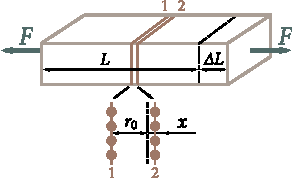
\includegraphics[scale=1]{figures/cap_02/fig_2_2.pdf}
		\caption[]{}
		\label{fig:2_2}
	\end{center}
\vspace{-0.7cm}
\end{figure}

Let us assume that the particles $m_1$ and $m_2$ are initially at rest at positions $1$ and $2$ (\fig{2_2}). The forces of interaction $\vec{F}_{12}$ and $\vec{F}_{21}$ are equal in magnitude and opposite in direction. Now assume that the particle $m_1$ moves very rapidly (with a speed almost equal to $c$) to position $1'$. At this point, the particle $m_1$ will experience the force $\vec{F}_{12}'$ smaller in magnitude ($r'>r$) and directed differently than $\vec{F}_{12}$ (we remind our reader that the field of the particle $m_2$ remains constant). The force $\vec{F}_{21}$ will continue to act on the second particle until the disturbance of the field due to the displacement of $m_1$ reaches point $2$. Consequently, Newton's third law was violated while the particle $m_1$ was in motion some time after it stopped at point $1'$.

If the particle $m_1$ moved from point $1$ to point $1'$ with the speed $v$ much smaller than $c$ ($v\ll c$), or the speed of propagation of field disturbances were infinitely great, then the instantaneous values of the field at point $2$ would correspond to the positions of the particle $m_1$ at the same moment of time, and, consequently, no violations of the third law would be observed.

Newtonian mechanics in general holds only for speeds that are much smaller than the speed of light (when $v\ll c$). Therefore, within the confines of this mechanics, the speed of propagation of field disturbances is considered to be infinite, and Newton's third law is always obeyed.

\section{Galileo's Relativity Principle}\label{sec:2_7}

Let us consider two reference frames moving relative to each other with the constant velocity $\vec{v}_0$. One of these frames, designated in~\fig{2_3} by the letter K, will conditionally be considered fixed. Therefore the second frame K$'$ will move uniformly in a straight line. Let us choose the coordinate axes $x, y, z$ of frame K and the axes $x',y',z'$ of frame K$'$ so that the axes $x$ and $x'$ coincide, while the axes $y$ and $y'$, and also $z$ and $z'$ are parallel to each other.

\begin{figure}[t]
	\begin{center}
		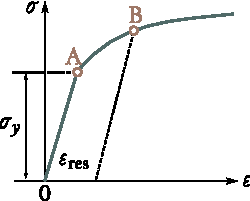
\includegraphics[scale=1]{figures/cap_02/fig_2_3.pdf}
		\caption[]{}
		\label{fig:2_3}
	\end{center}
	\vspace{-0.7cm}
\end{figure}

Let us find the relation between the coordinates $x, y, z$ of a point P in frame K and the coordinates $x', y', z'$ of the same point in frame K$'$. If we begin to count the time from the moment when the origins of the coordinates of the two frames coincided, then as follows from~\fig{2_3}, we have $x=x'+v_0t$. In addition, it is quite obvious that $y=y'$ and $z=z'$. Adding to these relations the assumption adopted in classical mechanics that the time flows the same in both frames, \ie, that $t=t'$, we get a group of four equations:
\begin{equation}\label{eq:2_19}
x=x'+v_0t,\quad y=y',\quad z=z',\quad t=t'.
\end{equation}

\noindent
They are called \textbf{Galilean transformations}.

The first and last of Eqs.~\eqref{eq:2_19} are correct only at values of $v_0$ that are small in comparison with the speed of light in a vacuum $c$ (\ie, $v_0\ll c$). At values of $v_0$ comparable with $c$, the Galilean transformations must be replaced with the more general Lorentz transformations (see Sec.~\ref{sec:8_2}). Equations~\eqref{eq:2_19} are assumed to be accurate within the confines of Newtonian mechanics.

Differentiating Eqs.~\eqref{eq:2_19} with respect to time, we find the relation between the velocities of point P relative to the reference frames K and K$'$:
\begin{align}
\dot{x} &= \dot{x}'+v_0, \quad\,\,\text{or}\quad\quad v_x=v_x'+v_0\nonumber\\
\dot{y} &= \dot{y}', \quad\quad\,\,\,\,\,\,\,\text{or}\quad\quad v_y=v_y'\label{eq:2_20}\\
\dot{z} &= \dot{z}', \quad\quad\,\,\,\,\,\,\,\,\text{or}\quad\quad v_z=v_z'.\nonumber
\end{align}

The three scalar relations~\eqn{2_20} are equivalent to the following relation between the velocity vector $\vec{v}$ relative to frame K and the velocity vector $\vec{v}'$ relative to frame K$'$:
\begin{equation}\label{eq:2_21}
\vec{v} = \vec{v}' + \vec{v}_0.
\end{equation}

\noindent
To convince ourselves in the truth of this equation, it is sufficient to project vector equation~\eqref{eq:2_21} onto the axes $x, y, z$. As a result, we get equations~\eqref{eq:2_20}.

Equations~\eqref{eq:2_20} and \eqref{eq:2_21} give the rule of velocity addition in classical mechanics. It must be borne in mind that~\eqn{2_21}, like any other vector equation, remains correct upon an arbitrary selection of the mutual directions of the coordinate axes of the frames K and K$'$. Equations~\eqref{eq:2_20}, however, are obeyed only when the axes are chosen as shown in~\fig{2_3}.

We noted in Sec.~\ref{sec:2_2} that any reference frame moving relative to an inertial frame with a constant velocity will also be inertial. Now we are in a position to prove this statement. To do this, let us differentiate~\eqn{2_21} with respect to time. Taking into account that $\vec{v}_0$ is constant, we get
\begin{equation}\label{eq:2_22}
\dot{\vec{v}} = \dot{\vec{v}}', \quad\text{or}\quad  \vec{a} = \vec{a}'.
\end{equation}

\noindent
Hence it follows that the acceleration of a body in all reference frames moving uniformly in a straight line relative to one another is the same. Therefore, if one of these frames is inertial (this signifies that in the absence of forces $\vec{a}=0$), then the others will also be inertial ($\vec{a}'$ also equals zero).

The fundamental equation of mechanics~\eqref{eq:2_21} is characterized by containing only the acceleration of the kinematic quantities. It does not contain the velocity. As we have established above, however, the acceleration of a body in two arbitrarily selected inertial reference frames K and K$'$ is the same. Hence it follows according to Newton's second law that the forces acting on a body in frames K and K$'$ will also be the same. Consequently, \textit{the equations of dynamics do not change upon transition from one inertial reference frame to another one}, \ie, they are said to be invariant with respect to the transformation of the coordinates corresponding to the transition from one inertial reference frame to another. From the viewpoint of mechanics, all inertial reference frames are absolutely equivalent, and none of them can be preferred to others. In practice, this manifests itself in that we cannot establish by any mechanical experiments conducted within the limits of a given reference frame whether it is in a state of rest or in uniform straight-line motion. For example, if we are in a car of a train running uniformly in a straight line without jolts we cannot determine whether the car is moving or at rest without looking out of a window. The free fall of bodies, the motion of objects that we throw, and all other mechanical processes in this case will occur in the same way as if the car were standing.

These circumstances were already established by Galileo Galilei (1564-1642). The statement that all mechanical phenomena in different inertial reference frames proceed identically, owing to which no mechanical experiments allow us to determine whether the given reference frame is at rest or is moving uniformly in a straight line, is called \textbf{Galileo's relativity principle}.

\section{Forces}\label{sec:2_8}

Four kinds of interactions are distinguished in modern physics: (1) gravitational (or interaction due to universal gravitation), (2) electromagnetic (achieved via electric and magnetic fields), (3) strong or nuclear (ensuring the binding of particles in an atomic nucleus), and (4) weak interaction (responsible for many processes of elementary particle decay).

Within the confines of classical mechanics, we have to do with gravitational and electromagnetic forces, and also with elastic and friction forces. The latter two kinds of forces are determined by the nature of the interaction between the molecules of a substance. The forces of interaction between molecules have an electromagnetic origin. Consequently, elastic and friction forces are electromagnetic in their nature.

Gravitational and electromagnetic forces are fundamental---they cannot be reduced to other simpler forces. Elastic and friction forces, on the other hand, are not fundamental.

The laws of the fundamental forces are exceedingly simple. The magnitude of the gravitational force is determined by~\eqn{2_18}. The magnitude of the force with which two point charges $q_1$ and $q_2$ at rest interact is determined by Coulomb's law:
\vspace{-12pt}
\begin{equation}\label{eq:2_23}
F = k\frac{q_1q_2}{r^2}
\end{equation}

\noindent
($k$ is a constant of proportionality depending on the units chosen for the quantities in the formula). 

If the charges are moving, then magnetic forces act on them in addition to the force defined by~\eqn{2_23}. The magnetic force acting on a point charge $q$ moving with the velocity $\vec{v}$ in a magnetic field of induction $\vec{B}$ is determined by the formula
\begin{equation}\label{eq:2_24}
\vec{F} = k'q\,(\vecprod{v}{B})
\end{equation}

\noindent
($k'$ is a constant of proportionality).

Equations~\eqref{eq:2_18}, \eqref{eq:2_23}, and \eqref{eq:2_24} are accurate ones. For elastic and friction forces we can obtain only approximate empirical formulas that are considered in the following sections.

\section{Elastic Forces}\label{sec:2_9}

Any real body becomes deformed, \ie, changes its dimensions and shape, under the action of forces applied to it. If the body regains its initial dimensions and shape after the action of the forces stops, the deformation or strain is called \textbf{elastic}. Elastic deformations are observed when the force producing the deformation does not exceed a definite limit, called the \textbf{elastic limit}, for each concrete body.

\begin{figure}[t]
	\begin{center}
		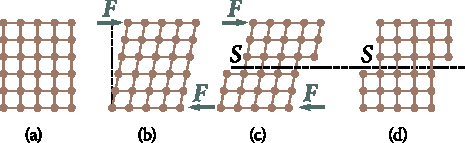
\includegraphics[scale=1]{figures/cap_02/fig_2_4.pdf}
		\caption[]{}
		\label{fig:2_4}
	\end{center}
	\vspace{-0.8cm}
\end{figure}

Let us take a spring of length $l_0$ in its undeformed state and apply the forces $\vec{F}_1$ and $\vec{F}_2$ to its ends that are equal in value and opposite in direction (\fig{2_4}). Under the action of these forces, the spring will stretch over a certain distance $\Delta l$, after which equilibrium will set in. In the state of equilibrium, the external forces $\vec{F}_1$ and $\vec{F}_2$ will be balanced by the elastic forces set up in the spring as a result of its deformation. Experiments show that with small deformations, the stretching of the spring $\Delta l$ is proportional to the stretching force: $\Delta l\propto F$ (here $F=F_1=F_2$). Accordingly, the elastic force is proportional to the elongation of the spring:
\begin{equation}\label{eq:2_25}
F = k\,\Delta l.
\end{equation}

\noindent
The constant of proportionality $k$ is called the \textbf{spring constant}.

The statement that the elastic force and deformation are proportional to each other is called \textbf{Hooke's law}.

Elastic strains are set up throughout the entire spring. Any part of the spring acts on another part with a force determined by~\eqn{2_25}. Therefore, if we cut the spring in half, an identical elastic force will appear in each half with the elongation being half the original value. Hence, we conclude that with a given material of the spring and a given coil size the magnitude of the elastic force is determined not by the absolute elongation of the spring $\Delta l$, but by its relative elongation $\Delta l/l_0$.

\begin{figure}[t]
	\begin{center}
		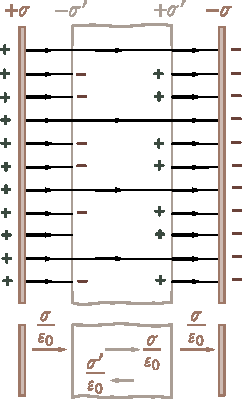
\includegraphics[scale=0.95]{figures/cap_02/fig_2_5.pdf}
		\caption[]{}
		\label{fig:2_5}
	\end{center}
	\vspace{-0.7cm}
\end{figure}

Elastic strains, but of the opposite sign, are also set up when a spring is compressed. Let us generalize~\eqn{2_25} as follows. We shall rigidly fix one end of a spring (\fig{2_5}) and shall consider the elongation of the spring as the coordinate $x$ of its other end measured from its position corresponding to the undeformed spring\footnote{In~\fig{2_5}b, the distance over which the end of the spring moved is designated $-x$. The reason is that the distance is a positive quantity, while the		coordinate $x$ in this case, however, is a negative one.}. In addition, by $F$ we shall understand the projection of the elastic force $\vec{F}_{\text{el}}$ onto the $x$-axis. We can thus write that
\begin{equation}\label{eq:2_26}
F = -k x
\end{equation}

(inspection of~\fig{2_5} shows that the projection of the elastic force onto the $x$-axis and the coordinate $x$ always have opposite signs).

%\begin{figure}[t]
%	\begin{minipage}[t]{0.5\linewidth}
%		\begin{center}
%			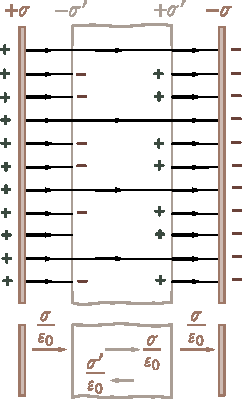
\includegraphics[scale=0.75]{figures/cap_02/fig_2_5.pdf}
%			\caption[]{}
%			\label{fig:2_5}
%		\end{center}
%	\end{minipage}
%	\hspace{-0.05cm}
%	\begin{minipage}[t]{0.5\linewidth}
%		\begin{center}
%			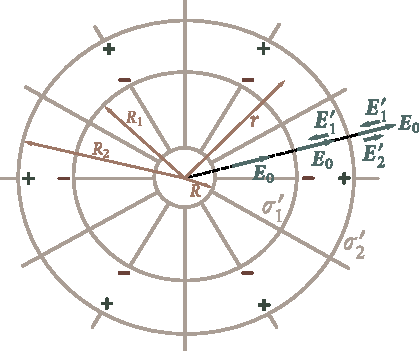
\includegraphics[scale=0.72]{figures/cap_02/fig_2_6.pdf}
%			\caption[]{}
%			\label{fig:2_6}
%		\end{center}
%	\end{minipage}
%	\vspace{-0.7cm}
%\end{figure}

Homogeneous bars behave in tension or uniaxial compression like a spring. If we apply the forces $\vec{F}_1$ and $\vec{F}_2$ ($F_1=F_2=F$) to the ends of a bar, these forces being directed along its axis and acting uniformly over the entire cross section, then the length of the bar $l_0$ will receive either a positive (in stretching) or a negative (in compression) increment\footnote{A change in the length of the bar is attended by a corresponding change in its cross-sectional dimensions.} $\Delta l$ (\fig{2_6}). It is quite natural to take the relative change in the length of the bar as the quantity characterizing its deformation:
\begin{equation}\label{eq:2_27}
\varepsilon = \frac{\Delta l}{l_0}.
\end{equation}

Experiments show that for bars of a given material the relative elongation or strain in elastic deformation is proportional to the force per unit cross-sectional area of the bar:
\begin{equation}\label{eq:2_28}
\varepsilon = \alpha\frac{\Delta l}{S}.
\end{equation}

\noindent
The constant of proportionality a is called the \textbf{compliance coefficient}.

\begin{figure}[t]
	\begin{center}
		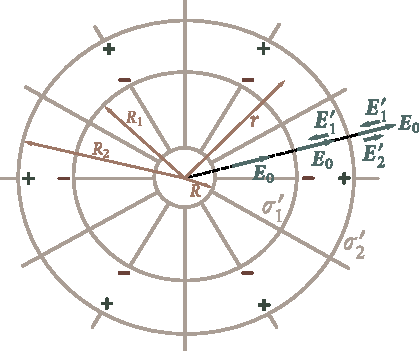
\includegraphics[scale=0.95]{figures/cap_02/fig_2_6.pdf}
		\caption[]{}
		\label{fig:2_6}
	\end{center}
	\vspace{-0.7cm}
\end{figure}

The quantity equal to the ratio between the force and the area of the surface it is acting on is called the stress. Owing to the interaction of the parts of a body with one another, the stress is transmitted to all points of the body---the entire volume of the body, for example a bar, will be in a stressed state. If the force is directed along a normal to the surface, the stress is called \textbf{normal}. If it is directed along a tangent to the surface it is acting on, the stress is called \textbf{tangential} (\textbf{shear}). The normal stress is designated by the symbol $\sigma$, the tangential or shear stress by the symbol $\tau$.

The ratio $F/S$ in~\eqn{2_28} is the normal stress $\sigma$. Hence, this equation can be written in the form
\begin{equation}\label{eq:2_29}
\varepsilon = \alpha\sigma.
\end{equation}

\noindent
In addition to the compliance coefficient $\alpha$, the elastic properties of a material are also characterized by its reciprocal $E=1/\alpha$, which is called the \textbf{modulus of elasticity} or \textbf{Young's modulus}. It is measured in pascals (the pascal is the unit of pressure in the SI system---$\SI{1}{\pascal}=\SI{1}{\newton\per\square\metre}$).

Using $1/E$ instead of $\alpha$ in~\eqn{2_9}, we get
\begin{equation}\label{eq:2_30}
\varepsilon = \frac{\alpha}{E}
\end{equation}

\noindent
from which it follows that Young's modulus equals such a normal stress at which the relative elongation or strain will equal unity (\ie, the increment of the length $\Delta l$ will be equal to the original length $l_0$) if so great elastic deformations were possible (actually a bar will fail at considerably smaller stresses, and the elastic limit is reached still earlier).

Solving~\eqn{2_28} with respect to $F$ and using $\Delta l/l_0$ instead of $\varepsilon$ and $1/E$ instead of $\alpha$, we get
\begin{equation}\label{eq:2_31}
F = \frac{E\,S}{l_0}\Delta l = k\,\Delta l
\end{equation}

\noindent
where $k$ is a constant quantity for a given bar. Equation~\eqref{eq:2_31} expresses Hooke's law for a bar [compare with~\eqn{2_26}]. Do not forget that this law is obeyed only until the elastic limit is reached. 

\begin{figure}[t]
	\begin{center}
		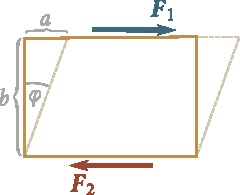
\includegraphics[scale=1]{figures/cap_02/fig_2_7.pdf}
		\caption[]{}
		\label{fig:2_7}
	\end{center}
	\vspace{-0.7cm}
\end{figure}

In conclusion, let us briefly consider shear strain. Let us take a homogeneous body having the shape of a rectangular parallelepiped and apply to its opposite faces the forces $\vec{F}_1$ and $\vec{F}_2$ ($F_1=F_2=F$) directed parallel to these faces (~\fig{2_7}). If the action of the forces is uniformly distributed over the entire surface of the corresponding face, then in any cross section parallel to these faces the tangential (shear) stress
\begin{equation}\label{eq:2_32}
\tau = \frac{F}{S}
\end{equation}

\noindent
will appear ($S$ is the area of a face). The action of the stresses will cause the body to deform so that one face will move relative to another over the distance $a$. If we mentally divide the body into elementary layers parallel to the faces we are considering, then each layer will be shifted with respect to its neighbours. For this reason, such deformation is called \textbf{shear}.

In shear, any straight line originally perpendicular to the layers will turn through the angle $\varphi$. Shear is characterized by the quantity
\begin{equation}\label{eq:2_33}
\gamma = \frac{a}{b} = \tan\varphi
\end{equation}

\noindent
called the \textbf{relative shear} (what $a$ and $b$ are is clear from~\fig{2_7}). Upon elastic deformations, the angle $\varphi$ is very small. We can therefore assume that $\tan\varphi\approx\varphi$. Consequently, the relative shear $\gamma$ equals the angle of shear $\varphi$.

Experiments show that the relative shear is proportional to the tangential stress:
\begin{equation}\label{eq:2_34}
\gamma = \frac{1}{G}\tau.
\end{equation}

\noindent
The coefficient $G$ depends only on the properties of a material and is called the \textbf{shear modulus}. It equals such a tangential (shear) stress at which the angle of shear will be 45 degrees ($\tan\varphi=1$) if the elastic limit were not exceeded at such great deformations. The shear modulus $G$, like Young's modulus $E$, is measured in pascals (\si{\pascal}).

\section{Friction Forces}\label{sec:2_10}

Forces of friction appear when contacting bodies or their parts move relative to one another. The friction occurring in the relative movement of two contacting bodies is called \textbf{external}; the friction between parts of the same continuous body (for example, a fluid) is called \textbf{internal}.

The force of friction appearing when a solid body moves relative to a fluid (liquid or gas) medium must be related to the category of internal friction forces because in this case the layers of the fluid in direct contact with the body are carried along with it at the body's velocity. The motion of the body is influenced by the friction between these layers of the fluid and other of its layers that are external relative to them.

Friction between the surfaces of two solids in the absence of any intermediate layer, for instance, a lubricant between them, is called \textbf{dry}. Friction between a solid and a fluid, and also between the layers of a fluid, is called \textbf{viscous} (or \textbf{liquid}).

Two kinds of dry friction are distinguished: \textbf{sliding} and \textbf{rolling}.

Forces of friction are directed along a tangent to the surfaces (or layers) in contact so that they resist the relative displacement of these surfaces (layers). If, for example, two layers of a liquid slide over each other with different velocities, then the force applied to the faster layer is directed oppositely to the direction of motion, while the force acting on the slower layer is directed along its motion.

\begin{figure}[t]
	\begin{center}
		\includegraphics[scale=1]{figures/cap_02/fig_2_8.pdf}
		\caption[]{}
		\label{fig:2_8}
	\end{center}
	\vspace{-0.7cm}
\end{figure}

\textbf{Dry Friction.} In dry friction, a force of friction appears not only when one surface slides over another one, but also when attempts are made to set up such sliding motion. In the latter case, we have to do with the \textbf{force of static friction}. Let us consider two contacting bodies $1$ and $2$ of which the latter is fixed in place (\fig{2_8}). Body $1$ is pressed against body $2$ by the force $\vec{F}_{\hatvec{n}}$ directed along a normal to the surface of contact of the bodies. It is called the \textbf{normal force} and may be due to the pressure of the body's weight, or to other reasons. Let us try to move body $1$ by acting on it with an external force $\vec{F}$. We shall find that for every concrete pair of bodies and every value of the normal force there is a definite minimum value $F_0$ of the force $\vec{F}$ at which body $1$ first begins to move. At values of the external force $F$ within the limits from $0$ to $F_0$, the body remains at rest. According to Newton's second law, this is possible if the force $\vec{F}$ is balanced by a force equalling it in magnitude and opposite in direction, which is exactly the force of static friction $\vec{F}_{\text{fr}}$ (see~\fig{2_8}). It automatically\footnote{This occurs in the same way as a spring acted upon by a stretching force automatically acquires an elongation such that the elastic force balances the external one.} acquires a value equal to that of the external force $F$ (provided that the latter does not exceed $F_0$). The quantity $F_0$ is the maximum possible value of the force of static friction.

It must be noted that in accordance with Newton's third law body $2$ must also experience the force of static friction $\vec{F}_{\text{fr}}'$ (it is shown by a dashed arrow in~\fig{2_8}) equal in magnitude to the force $\vec{F}_{\text{fr}}$ but directed oppositely.

If the external force $\vec{F}$ exceeds $F_0$ in magnitude, the body begins to slide. Its acceleration is determined by the resultant of two forces: the external one $\vec{F}$ and the force of sliding friction $\vec{F}_{\text{fr}}$ whose magnitude depends to a certain extent on the sliding speed. The nature of this relation is determined by the nature and state of the contacting surfaces. The kind of the speed dependence of the force of friction shown in~\fig{2_9} is encountered most frequently. The graph shows both static and sliding friction. The force of static friction, as we have already noted, may range from $0$ to $F_0$, which is shown by the vertical line in the graph. In accordance with~\fig{2_9}, the force of sliding friction first diminishes somewhat with increasing speed, and then begins to grow. With special processing of contacting surfaces, the force of sliding friction may be virtually independent of the speed. In this case, the curved portion of the graph in~\fig{2_9} will transform into a horizontal line beginning at the point $F_0$.

\begin{figure}[t]
	\begin{center}
		\includegraphics[scale=0.98]{figures/cap_02/fig_2_9.pdf}
		\caption[]{}
		\label{fig:2_9}
	\end{center}
	\vspace{-0.7cm}
\end{figure}

The laws of dry friction consist in the following: the maximum force of static friction, and also the force of sliding friction do not depend on the area of contact between bodies and are approximately proportional to the magnitude of the normal force pressing the contacting surfaces together:
\begin{equation}\label{eq:2_35}
F_{\text{fr}} = f\,F_{\hatvec{n}}.
\end{equation}

\noindent
The dimensionless proportionality constant $f$ is called the \textbf{coefficient of friction} (static or sliding friction, as the case may be). It depends on the nature and state of the contacting surfaces, particularly on their roughness. The coefficient of sliding friction is a function of speed.

Friction forces play a very great part in nature. Friction is often a great help to us in our everyday life. Let us remember the tremendous difficulties encountered by pedestrians and vehicles on ice-covered pavements and roads, when the friction between the pavement surface and the pedestrians' soles or the wheels of the vehicles considerably diminishes. If there were no friction forces, our furniture would have to be fastened to the floor like on a ship on a rolling sea because upon the most minute deviation of the floor from a horizontal position it would slide in the direction of the slope. Our reader can give numerous similar examples of how helpful friction is.

The part played by friction is often extremely negative, and measures have to be taken to reduce it as much as possible. This relates, for example, to the friction in bearings or between the hub of a wheel and an axle.

The most radical way of reducing forces of friction is to replace sliding friction with rolling friction. The latter appears, for example, between a cylindrical or spherical body rolling over a flat or curved surface. Rolling friction formally obeys the same laws as sliding friction, but the coefficient of friction in this case is much lower.

\textbf{Viscous Friction and Resistance of the Medium.} Unlike dry friction, viscous (internal) friction is characterized by the force of viscous friction vanishing together with the velocity. Therefore, no matter how small an external force is, it can impart a relative velocity to the layers of a viscous medium. The laws which the forces of friction between the layers of a medium obey will be considered in the chapter devoted to fluid mechanics (Chap.~\ref{chap:9}). 

\begin{figure}[t]
	\begin{center}
		\includegraphics[scale=1]{figures/cap_02/fig_2_10.pdf}
		\caption[]{}
		\label{fig:2_10}
	\end{center}
	\vspace{-0.7cm}
\end{figure}

In this section, we shall limit ourselves to a treatment of the friction forces between a solid and a viscous (fluid) medium. It must be borne in mind that apart from the forces of friction proper, the motion of bodies in a fluid is attended by the so-called forces of \textbf{resistance of the medium} that can be much greater than the forces of friction. We have no possibility of considering the causes of these forces in detail. We shall only treat the laws obeyed jointly by forces of friction and resistance of the medium. We shall conditionally call the total force the force of friction. The speed dependence of this force is shown in~\fig{2_10}.

At low velocities, the force grows linearly with the velocity:
\begin{equation}\label{eq:2_36}
\vec{F}_{\text{fr}} = -k_1 \vec{v}
\end{equation}

\noindent
(the minus sign signifies that the force is directed oppositely to the velocity). The value of the coefficient $k_1$ depends on the shape and dimensions of a body, the state of its surface, and on the property of the fluid called its viscosity. For example, this coefficient is much higher for glycerine than for water.

At high velocities, the linear law transforms into a quadratic one, \ie, the force begins to grow in proportion to the square of the velocity:
\begin{equation}\label{eq:2_37}
\vec{F}_{\text{fr}} = -k_2\, v^2\, \vecuni{v}
\end{equation}

\noindent
($\vecuni{v}$ is the unit vector of the velocity). The value of the coefficient $k_2$ depends on the shape and dimensions of a body.

The magnitude of the velocity at which the law~\eqref{eq:2_36} transforms into~\eqref{eq:2_37} depends on the shape and dimensions of a body, and also on the viscosity and density of the fluid.

\section{Force of Gravity and Weight}\label{sec:2_11}

The force of attraction to the Earth causes all bodies to fall with the same acceleration relative to the Earth's surface, which is designated by the symbol $g$. This signifies that in a reference frame associated with the Earth, any body of mass $m$ is acted upon by the force
\begin{equation}\label{eq:2_38}
\vec{P} = m\vec{g}
\end{equation}

\noindent
called the force of gravity\footnote{Owing to the non-inertial nature of a reference frame associated with the Earth, the force of gravity will differ somewhat from the force with which a body is attracted to the Earth. This will be treated in greater detail in Sec.~\ref{sec:4_2}.}. When a body is at rest relative to the Earth's surface, the force $\vec{P}$ is balanced by the reaction\footnote{Reactions are forces with which a given body is acted upon by bodies restricting its motion.} $\vec{F}_{\text{r}}$ of the suspension or support preventing falling of the body ($\vec{F}_{\text{r}}=-\vec{P}$). According to Newton's third law, the body in this case acts on the suspension or support with the force $\vec{W}$ equal to $-\vec{F}_{\text{r}}$, \ie, with the force
\begin{equation*}
\vec{W} = \vec{P} = m\vec{g}
\end{equation*}

\begin{figure}[t]
	\begin{center}
		\includegraphics[scale=1]{figures/cap_02/fig_2_11.pdf}
		\caption[]{}
		\label{fig:2_11}
	\end{center}
	\vspace{-0.7cm}
\end{figure}

The force $\vec{W}$ with which a body acts on its suspension or support is called the \textbf{weight of the body}. This force equals $m\vec{g}$ only when the body and its support (or suspension) are stationary relative to the Earth. If they are moving with a certain acceleration $\vec{a}$, their weight $\vec{W}$ will not equal $m\vec{g}$. This can be explained by the following example. Let a suspension in the form of a spring fastened to a frame move together with a body with the acceleration $\vec{a}$ (\fig{2_11}). The equation of motion of the body will therefore have the form
\begin{equation}\label{eq:2_39}
\vec{P} + \vec{F}_{\text{r}} = m\vec{a}
\end{equation}

\noindent
where $\vec{F}_{\text{r}}$ is the reaction of the suspension, \ie, the force with which the spring acts on the body. According to Newton's third law, the body acts on the spring with a force equal to $-\vec{F}_{\text{r}}$, which by definition is the weight of the body $\vec{W}$ in these conditions. Substituting the force $-\vec{W}$ for the reaction $\vec{F}_{\text{r}}$ and the product $m\vec{g}$ for the force of gravity $\vec{P}$ in~\eqn{2_39}, we get
\begin{equation}\label{eq:2_40}
\vec{W} = m(\vec{g} - \vec{a}).
\end{equation}

\noindent
Equation~\eqref{eq:2_40} determines the weight of a body in the general case. It holds for a suspension or a support of any kind.

Let us assume that our body and the suspension are moving in a vertical direction (\fig{2_11} is based on this assumption).

We project~\eqn{2_40} onto the direction of a plumb line:
\begin{equation}\label{eq:2_41}
W = m(g \pm a).
\end{equation}

\noindent
In this expression, $W$, $g$, and $a$ are the magnitudes of the corresponding vectors. The plus sign corresponds to a directed upward, and the minus sign to a directed downward.

It follows from~\eqn{2_41} that the magnitude of the weight $\vec{W}$ may be either greater or smaller than the force of gravity $\vec{P}$. In free fall of the frame with the suspension, $\vec{a}=\vec{g}$, and the force $\vec{W}$ with which the body acts on the suspension vanishes. A state of weightlessness sets in. A spaceship orbiting around the Earth with its engines switched off travels, like the freely falling frame, with the acceleration $\vec{g}$. As a result, the bodies inside it are in a state of weightlessness---they exert no pressure on the bodies in contact with them.

It must be noted that the force of gravity $\vec{P}$ is often confused with the weight of a body $\vec{W}$. This is due to the fact that with a stationary support, the forces $\vec{P}$ and $\vec{P}$ coincide both in magnitude and in direction (they both equal $m\vec{g}$). It must be remembered, however, that these forces are applied to different bodies: $\vec{P}$ is applied to a body itself, whereas $\vec{W}$ is applied to the suspension or support restricting the free motion of the body in the field of the Earth's gravitational forces. In addition, the force $\vec{P}$ always equals $m\vec{g}$ regardless of whether the body is moving or at rest, whereas the force of weight $\vec{W}$ depends on the acceleration with which the support and the body are moving. It may be either greater or smaller than $m\vec{g}$, and, in particular, in a state of weightlessness it vanishes.

The relation~\eqref{eq:2_40} between the mass and the weight of a body provides a way of comparing the masses of bodies by weighing them: the ratio of the weights of bodies determined in identical conditions (usually at $\vec{a}=0$) at the same point on the Earth's surface equals the ratio of the masses of these bodies:
\begin{equation*}
W_1\,:\,W_2\,:\,W_3\,:\,\ldots = m_1\,:\,m_2\,:\,m_3\ldots.
\end{equation*}

It will be shown in Sec.~\ref{sec:4_2} that the acceleration of free fall $g$ and the force of gravity $P$ depend on the latitude of a locality. They also depend on the altitude, and diminish with an increasing distance from the centre of the Earth.

\section{Practical Application of Newton's Laws}\label{sec:2_12}

\begin{figure}[t]
	\begin{center}
		\includegraphics[scale=1]{figures/cap_02/fig_2_12.pdf}
		\caption[]{}
		\label{fig:2_12}
	\end{center}
	\vspace{-0.7cm}
\end{figure}

To compile an equation of motion, we must first of all establish what forces act on the body being considered. It is necessary to determine the action of other bodies on the given one that must be taken into account. For example, for a body sliding down an inclined plane (\fig{2_12}), the action exercised by the Earth is important (it is characterized by the force $m\vec{g}$), and also the action exercised by the plane (it is characterized by the force of the reaction $\vec{F}_{\text{r}}$).

Never take into account ``moving'', ``rolling down'', ``centripetal'', ``centrifugal''\footnote{This does not relate to the term ``centrifugal force of inertia'' (see Sec.~\ref{sec:4_2}.} and similar forces. To prevent an error, characterize a force according to the ``source'' causing it to appear, and not according to the action it produces. This means that behind every force we must see the body whose action sets up the force. This will eliminate the typical error consisting in that the same force is taken into account twice under different names.

In the example we are considering (see~\fig{2_12}), it is good to resolve the force of the reaction $\vec{F}_{\text{r}}$ into two components---the normal force $\vec{F}_{\hatvec{n}}$ and the friction force $\vec{F}_{\text{fr}}$. This, in particular, is useful in connection with the fact that the force of friction is proportional to the magnitude of the force $\vec{F}_{\hatvec{n}}$ [see~\eqn{2_35}].

Having determined the forces acting on a body, we write an equation of Newton's second law. In our example, it has the form
\begin{equation}\label{eq:2_42}
m\vec{a} = m\vec{g} + \vec{F}_{\text{r}} = m\vec{g} + \vec{F}_{\hatvec{n}} + \vec{F}_{\text{fr}}.
\end{equation}

\noindent
To perform calculations, we must pass over from vectors to their projections onto the correspondingly chosen directions, using the following properties of projections:
\begin{enumerate}[(1)]
	\item equal vectors have identical projections;
	\item the projection of a vector obtained by multiplying another vector by a scalar equals the product of the projection of this second vector and the scalar;
	\item the projection of a sum of vectors equals the sum of the projections of the vectors being added [see~\eqn{1_8}].
\end{enumerate}

Let us project the vectors in~\eqn{2_42} onto the direction $x$ shown in~\fig{2_12}. The projections of the vectors are $a_x=a$ ($a$ is the magnitude of the vector $\vec{a}$), $g_x=g\sin\alpha$, $F_{\hatvec{n}x}=0$, $F_{\text{r}x}=-f F_{\hatvec{n}x}=-fmg\cos\alpha$. Consequently, we arrive at the equation
\begin{equation*}
ma = mg\sin\alpha - fmg\cos\alpha
\end{equation*}

\noindent
from which it is a simple matter to find $a$.

In more complicated cases, we have to project the vectors onto several directions and solve the resulting system of algebraic or differential equations.

\cleardoublepage
% !TEX root = saveliev_physics_general_course_1.tex
%!TEX TS-program = pdflatex
%!TEX encoding = UTF-8 Unicode


\chapter{LAWS OF CONSERVATION}\label{chap:3}

\section{Quantities Obeying the Laws of Conservation}\label{sec:3_1}

Bodies forming a mechanical system may interact with one another and with bodies not belonging to the given system. Accordingly, the forces acting on the bodies of a system can be divided into \textbf{internal} and \textbf{external} ones. We shall define internal forces as the forces with which a given body is acted upon by the other bodies of the system, and external forces as those produced by the action of bodies not belonging to the system. If external forces are absent, the relevant system is called \textbf{closed}.

There are functions of the coordinates and velocities of the particles\footnote{We remind our reader that by a particle here we mean a point particle.} forming a system for closed systems that retain constant values upon motion. These functions are called motion integrals.

The number of motion integrals that can be formed for a system of $N$ particles between which there are no rigid constraints is $6N-1$. Only those of them are of interest to us that have the property of additivity. This property consists in that the value of a motion integral for a system comprising parts whose interaction may be disregarded equals the sum of the values for each part. There are three additive motion integrals. The first is called \textbf{energy}, the second---\textbf{momentum}, and the third---\textbf{angular momentum}.

Thus, three physical quantities do not change in closed systems, namely, energy, momentum, and angular momentum. Accordingly, there are three \textbf{laws of conservation}---that of energy conservation, that of momentum conservation, and that of angular momentum conservation. These laws are closely associated with the fundamental properties of space and time.

The conservation of energy is based on the \textbf{uniformity of time}, \ie, the equivalence of all moments of time. The equivalence should be understood in the sense that the substitution of the moment of time $t_2$ for the moment $t_1$ without a change in the values of the coordinates and velocities of the particles does not change the mechanical properties of a system. This signifies that after such a substitution, the coordinates and velocities of the particles have the same values at any moment of time $t_2+t$ as they would have had before the substitution at the moment $t_1+t$.

The conservation of momentum is based on the uniformity of space, \ie, the identical properties of space at all points. This should be understood in the sense that a translation of a closed system from one place in space to another without changing the mutual arrangement and velocities of the particles does not change the mechanical properties of the system (it is assumed that the closed nature of the system is not violated at the new place).

Finally, the conservation of angular momentum is based on the \textbf{isotropy of space}, \ie, the identical properties of space in all directions. This should be understood in the sense that rotation of a closed system as a whole does not affect its mechanical properties.

The laws of conservation are a powerful means of research. It is often extremely difficult to accurately solve equations of motion. In these cases, the laws of conservation permit us to obtain numerous important data on how mechanical phenomena proceed without having to solve equations of motion. The laws of conservation do not depend on the nature of the acting forces. This is why they can help us obtain much important information on the behaviour of mechanical systems even when the forces are unknown.

In the following sections, we shall obtain the laws of conservation on the basis of Newton's equations. It must be borne in mind, however, that the laws of conservation have a much more general nature than Newton's laws. The laws of conservation remain strictly correct even when Newton's laws (particularly the third one) are violated. We stress the fact that the laws of energy, momentum, and angular momentum conservation are accurate laws that are also strictly obeyed in the relativistic realm.

\section{Kinetic Energy}\label{sec:3_2}

Let us now pass over to finding the additive integrals of motion. We shall first consider the simplest system consisting of a single point particle.

The equation of motion of the particle is
\begin{equation}\label{eq:3_1}
m\dot{\vec{v}} = \vec{F}.
\end{equation}

\noindent
Here $\vec{F}$ is the resultant of the forces acting on the particle. Multiplying \eqn{3_1} by the displacement of the particle $\mathrm{d}\vec{s}=\vec{v}\,\mathrm{d}t$, we get
\begin{equation}\label{eq:3_2}
m\vec{v}\dot{\vec{v}}\,\mathrm{d}t = \vec{F}\,\mathrm{d}\vec{s}.
\end{equation}

\noindent
The product $\dot{\vec{v}}\,\mathrm{d}t$ is the increment of the velocity of the particle $\mathrm{d}\vec{v}$ during the time $\mathrm{d}t$. Accordingly
\begin{equation}\label{eq:3_3}
m\vec{v}\dot{\vec{v}}\,\mathrm{d}t = m\vec{v}\,\mathrm{d}\vec{v} = m\,\mathrm{d}\!\left(\frac{v^2}{2}\right) = \mathrm{d}\!\left(\frac{mv^2}{2}\right)
\end{equation}

\noindent
%[see \eqn{2_50}].
Performing such a substitution in \eqn{3_2}, we arrive at the expression
\begin{equation}\label{eq:3_4}
\mathrm{d}\!\left(\frac{mv^2}{2}\right) = \vec{F}\,\mathrm{d}\vec{s}.
\end{equation}

\noindent
If the system is closed, \ie, $\vec{F}=0$, then $\mathrm{d}(mv^2/2)=0$, while the quantity
\begin{equation}\label{eq:3_5}
E_{\text{k}} = \frac{mv^2}{2}
\end{equation}

\noindent
itself remains constant. This quantity is called the \textbf{kinetic energy} of the particle. For an isolated particle, the kinetic energy is an integral of motion\footnote{For a single isolated particle, any power of the velocity remains constant. But for a system of several interacting particles, it is exactly quantities of the form of \eqn{3_5} that are addends in the additive integral of motion.}.

Multiplying the numerator and denominator of \eqn{3_5} by $m$ and taking into consideration that the product $mv$ equals the momentum $p$ of a body, the expression for the kinetic energy can be given the form
\begin{equation}\label{eq:3_6}
E_{\text{k}} = \frac{p^2}{2m}.
\end{equation}

\noindent
If the force $\vec{F}$ acts on a particle, its kinetic energy does not remain constant. In this case in accordance with \eqn{3_4}, the increment of the particle's kinetic energy during the time $\mathrm{d}t$ equals the scalar product $\vec{F}\,\mathrm{d}\vec{s}$ ($\mathrm{d}\vec{s}$ is the displacement of the particle during the time $\mathrm{d}t$). The quantity
\begin{equation}\label{eq:3_7}
\mathrm{d}A = \vec{F}\,\mathrm{d}\vec{s}
\end{equation}

\noindent
is called the \textbf{work} done by the force $\vec{F}$ over the path $\mathrm{d}s$ ($\mathrm{d}s$ is the magnitude of the displacement $\mathrm{d}\vec{s}$). The scalar product~\eqref{eq:3_7} can be represented as the product of the projection of the force onto the direction of the displacement $F_{\text{s}}$ and the elementary distance $\mathrm{d}s$. Consequently, we can write that
\begin{equation}\label{eq:3_8}
\mathrm{d}A = F_{\text{s}}\,\mathrm{d}s.
\end{equation}

\noindent
It is clear from the above that work characterizes the change in energy due to the action of a force on a moving particle.

Let us integrate \eqn{3_4} along a certain trajectory from point $1$ to point $2$:
\begin{equation*}
\int_{1}^{2} \mathrm{d}\!\left(\frac{mv^2}{2}\right) = \int_{1}^{2} \vec{F}\,\mathrm{d}\vec{s}.
\end{equation*}

\noindent
The left-hand side is the difference between the values of the kinetic energy at points $2$ and $1$, \ie, the increment\footnote{The change in a quantity $a$ can be characterized either by its increment or its decrement. The increment of the quantity $a$, which we shall designate by $\Delta a$ is defined as the difference between the final ($a_2$) and initial ($a_1$) values of this quantity: $\text{increment}=\Delta a=a_2-a_1$. The decrement of the quantity a is the difference between its initial ($a_1$) and final ($a_2$) values: $\text{increment}=a_1-a_2=-\Delta a$. The decrement of a quantity equals its ·increment with the opposite sign. The increment and decrement are algebraic quantities.} of the kinetic energy along path $1$-$2$. Taking this into account, we get:
\begin{equation}\label{eq:3_9}
E_{\text{k},2} - E_{\text{k},1} = \frac{mv^2_2}{2} - \frac{mv^2_1}{2} = \int_{1}^{2} \vec{F}\,\mathrm{d}\vec{s}.
\end{equation}

The quantity
\begin{equation}\label{eq:3_10}
A = \int_{1}^{2} \vec{F}\,\mathrm{d}\vec{s} = \int_{1}^{2} F_{\text{s}}\,\mathrm{d}s
\end{equation}

\noindent
is the work of the force $\vec{F}$ over path $1$-$2$. We shall sometimes denote this work by the symbol $A_{12}$ instead of $A$.

Thus, \textit{the work of the resultant of all the forces acting on a particle produces an increment of the particle's kinetic energy}:
\begin{equation}\label{eq:3_11}
A_{12} = E_{\text{k},2} - E_{\text{k},1}.
\end{equation}

\noindent
It follows from \eqn{3_11} that energy has the same dimension as work. Accordingly, energy is measured in the same units as work (see the following section).

\section{Work}\label{sec:3_3}

Let us consider the quantity that we called work in greater detail. Equation~\eqref{eq:3_7} can be written in the form
\begin{equation}\label{eq:3_12}
\mathrm{d}A = \vec{F}\,\mathrm{d}\vec{s} = F\cos\alpha\,\deriv{s}
\end{equation}

\noindent
where $\alpha$ is the angle between the direction of the force and that of the displacement of the point of application of the force.

If the force and the direction of the displacement make an
acute angle ($\cos\alpha>0$), the work is positive. If the angle $\alpha$ is obtuse ($\cos\alpha<0$), the work is negative. When $\alpha=\pi/2$, the work equals zero. This especially clearly shows that the concept of work in mechanics appreciably differs from our ordinary notion of it. In the ordinary meaning, any effort, particularly muscular strain, is always attended by work being done. For example, in order to hold a heavy load while standing still, and, moreover, to carry this load along a horizontal path, a porter spends much effort, \ie, ``does work''. The work as a mechanical quantity in these cases, however, equals zero.

\begin{figure}[t]
	\begin{center}
		\includegraphics[scale=1]{figures/ch_03/fig_3_1.pdf}
		\caption[]{}
		\label{fig:3_1}
	\end{center}
	\vspace{-0.7cm}
\end{figure}

Figure~\ref{fig:3_1} is a plot of the projection of the force onto the direction of displacement $F_{\text{s}}$ as a function of the position of the particle on its trajectory (the axis of abscissas has been taken as the $s$-axis, the length of the part of this axis between points $1$ and $2$ equals the total length of the path). Examination of the figure shows that the elementary work $\deriv{A}=F_{\text{s}}\,\deriv{s}$ equals numerically the area of the shaded strip, while the work $A$ over path $1$-$2$ equals numerically the area of the figure confined by the curve $F_{\text{s}}$, the vertical lines from points $1$ and $2$ and the $s$-axis (compare with \fig{1_26}).

Let us use this result to find the work done in the deformation of a spring obeying Hooke's law [see \fig{2_5} and \eqn{2_26}]. We shall begin with stretching of the spring. We shall do this very slowly so that the force $\vec{F}_{\text{ext}}$ which we act on the spring with may be considered equal in magnitude to the elastic force $\vec{F}_{\text{el}}$ all the time. Hence, $\vec{F}_{x,\text{ext}}=-\vec{F}_{x,\text{el}}=kx$, where $x$ is the elongation of the spring (\fig{3_2}). A glance at the figure shows that the work required to cause the elongation $x$ of the spring is
\begin{equation}\label{eq:3_13}
A = \frac{kx^2}{2}.
\end{equation}

\noindent
When the spring is compressed by the amount $x$, work of the same magnitude and sign is done as in stretching by $x$. The projection of the force $\vec{F}_{\text{ext}}$ in this case is negative ($\vec{F}_{\text{ext}}$ is directed to the left, $x$ grows to the right, see \fig{3_2}), and all the $\deriv{x}$'s are also negative. As a result, the product $\vec{F}_{x,\text{ext}}\,\deriv{x}$ is positive.

\begin{figure}[t]
	\begin{center}
		\includegraphics[scale=0.95]{figures/ch_03/fig_3_2.pdf}
		\caption[]{}
		\label{fig:3_2}
	\end{center}
	\vspace{-0.7cm}
\end{figure}

In a similar way, we can find an expression for the work done upon the elastic stretching or compression of a bar. According to \eqn{2_31}, this work is
\begin{equation}\label{eq:3_14}
A = \frac{1}{2}\frac{ES}{l_0}(\Delta l)^2 = \frac{1}{2}ESl_0\left(\frac{\Delta l}{l_0}\right)^2 = \frac{1}{2}EV\varepsilon^2
\end{equation}

\noindent
where $V=Sl_0$ is the volume of the bar, and $\varepsilon=\Delta l/l_0$ is the relative elongation [see \eqn{2_27}].

Assume that several forces whose resultant is $\vec{F}=\sum_{i}\vec{F}_i$ act simultaneously on a body. It follows from the distributivity of a scalar product of vectors [see \eqn{1_20}] that the work $\deriv{A}$ done by the resultant force over the path $\deriv{s}$ can be represented in the form
\begin{equation}\label{eq:3_15}
\deriv{A} = \left(\sum_{i}\vec{F}_i\right)\deriv{s} = \sum_{i}\vec{F}_i\,\deriv{\vec{s}} = \sum_{i}\deriv{A}_i.
\end{equation}

\noindent
This signifies that the work of the resultant of several forces equals the algebraic sum of the work done by each force separately.

The elementary displacement $\deriv{\vec{s}}$ can be represented as $\vec{v}\deriv{t}$. We can therefore write the expression for the elementary work in the form
\begin{equation}\label{eq:3_16}
\deriv{A} = \vec{F}\vec{v}\,\deriv{t}.
\end{equation}

\noindent
The work done during the interval from $t_1$ to $t_2$ can thus be calculated by the formula
\begin{equation}\label{eq:3_17}
A = \int_{t_1}^{t_2}\vec{F}\,\deriv{t}.
\end{equation}

In accordance with \eqn{1_21}, we have $\vec{F}\,\deriv{\vec{s}}=F\,\deriv{s_F}$, where $\deriv{s_F}$, is the projection of the elementary displacement $\deriv{\vec{s}s}$ onto the direction of the force $\vec{F}$. The formula for work can therefore be written as follows:
\begin{equation}\label{eq:3_18}
\deriv{A} = F\,\deriv{s_F}.
\end{equation}

\begin{figure}[t]
	\begin{center}
		\includegraphics[scale=0.95]{figures/ch_03/fig_3_3.pdf}
		\caption[]{}
		\label{fig:3_3}
	\end{center}
	\vspace{-0.7cm}
\end{figure}

If the force has a constant magnitude and direction (\fig{3_3}), then the vector $\vec{F}$ in the expression for work may be put outside the integral. The result is
\begin{equation}\label{eq:3_19}
A = \vec{F}\int_{1}^{2}\deriv{\vec{v}} = \vecdot{F}{s} = F s_F
\end{equation}

\noindent
where $\vec{s}$ is the vector of the displacement from point $1$ to point $2$, and $s_F$ is its projection onto the direction of the force.

The work done in unit time is called power. If the work $\deriv{A}$ is done in the time $\deriv{t}$, then the power is
\begin{equation}\label{eq:3_20}
P = \diff{A}{t}.
\end{equation}

\noindent
Taking $\deriv{A}$ as given by \eqn{3_16}, we get the following expression for the power:
\begin{equation}\label{eq:3_21}
P = \vecdot{F}{v}
\end{equation}

\noindent
according to which the power equals the scalar product of the force vector and the vector of the velocity with which the point of application of the force is moving.

\textbf{Units of Work and Power.} The unit of work is the work done by a force equal to unity and acting in the direction of the displacement over a unit distance. Consequently,
\begin{enumerate}[(1)]
	\item in the SI system, the unit of work is the joule (\si{\joule})---the work done by a force of \SI{1}{\newton} over a distance of \SI{1}{\metre};
	\item in the cgs system, the relevant unit is the \si{\erg}---the work done by a force of \SI{1}{\dyne} over a distance of \SI{1}{\centi\metre};
	\item in the mkg(force)s system, the unit is the kilogramme(force)m (\si{\kgf\metre})---the work done by a force of \SI{1}{\kgf} over a distance of \SI{1}{\metre}.
\end{enumerate}

The units of work are related as follows:
\begin{align*}
&\SI{1}{\joule} = \SI{1}{\newton}\times\SI{1}{\metre} = \SI{e5}{\dyne}\times\SI{e2}{\centi\metre} = \SI{e7}{\erg}\\
&\SI{1}{\kgf\metre} = \SI{1}{\kgf}\times\SI{1}{\metre} = \SI{9.81}{\newton}\times\SI{1}{\metre} = \SI{9.81}{\joule}.
\end{align*}

The unit of power is the power at which 1 unit of work is done in unit time. The unit of power in the SI system is the watt (\si{\watt}) equal to one joule per second (\si{\joule\per\second}). The unit of power in the cgs system (\si{\erg\per\second}) has no special name. The relation between the watt and the \si{\erg\per\second} is $\SI{1}{\watt}=\SI{e7}{\erg\per\second}$.

The unit of power in the mkg{force)s system is the (metric) horsepower (\si{\hp}), equal to \SI{75}{\kgf\metre\per\second}, $\SI{1}{\hp}=\SI{736}{\watt}$ (do not confuse this unit with the British or U.S. horsepower equal to \num{550}~ft-lb \si{\per\second} or \SI{746}{\watt}).

A system of prefixes is used, especially in the SI system, to denote multiples and submultiples of units. The names and symbols of these prefixes and the relevant factor by which the basic unit is multiplied are indicated in Table~\ref{table:3_1}.

\begin{table}[!b]
	\renewcommand{\arraystretch}{1.2}
	\caption{Prefixes for Multiples and Submultiples of Units}
	\vspace{-0.6cm}
	\label{table:3_1}
	\begin{center}\resizebox{0.95\linewidth}{!}{
			\begin{tabular}{lcclcc}
				\toprule[1pt]
				& & \textbf{Factor by which} & & & \textbf{Factor by which}\\
				\textbf{Name} & \textbf{Symbol} & \textbf{unit is multiplied} & \textbf{Name} & \textbf{Symbol} & \textbf{unit is multiplied}\\
				\midrule[0.5pt]\midrule[0.5pt]
				Tera & T & \num{e12} & Centi & \si{\centi} & \num{e-2}\\
				Giga & G & \num{e9}  & Milli & \si{\milli} & \num{e-3}\\
				Mega & M & \num{e6}  & Micro & \si{\micro} & \num{e-6}\\
				Kilo & k & \num{e3}  & Nano & \si{\nano} & \num{e-9}\\
				Hecto & h & \num{e2}  & Pico & \si{\pico} & \num{e-12}\\
				Deca & da & \num{e1}  & Femto & \si{\femto} & \num{e-15}\\
				Deci & d & \num{e-1}  & Atto & \si{\atto} & \num{e-18}\\
				\bottomrule[1pt]
			\end{tabular}
			%	\end{center}
	}\end{center}
\end{table}

For example, the unit of work called the megajoule is equivalent to \num{e6} joules ($\SI{1}{\mega\joule}=\SI{e6}{\joule}$), and the unit of power called the microwatt is equivalent to \num{e-6} watt ($\SI{1}{\micro\watt}=\SI{e-6}{\watt}$}. Similarly, \num{1} micrometer (formerly called the micron) is equivalent to \SI{e-6}{\metre} ($\SI{1}{\micro\metre}=\SI{e-6}{\metre}$), and $\SI{1}{\pico\newton}=\SI{e-12}{\newton}$.

\section{Conservative Forces}\label{sec:3_4}

If a particle is subjected to the action of other bodies at every point of space, the particle is said to be in a field of forces. For example, a particle near the Earth's surface is in the field of gravity forces---at every point of space the force $\vec{P}=m\vec{g}$ acts on it.

\begin{figure}[t]
	\begin{center}
		\includegraphics[scale=1]{figures/ch_03/fig_3_4.pdf}
		\caption[]{}
		\label{fig:3_4}
	\end{center}
	\vspace{-0.7cm}
\end{figure}

Let us consider as a second example the charged particle $e$ in the electric field set up by the fixed point charge $q$ (\fig{3_4}). A feature of this field is that the direction of the force acting on the particle at any point of space passes through a fixed centre (the charge $q$), while the magnitude of the force depends only on the distance to this centre, \ie, $F=F(r)$ [see \eqn{2_23}]. A field of forces with such properties is called a \textbf{central} one.

If at every point of a field the force acting on a particle is identical in magnitude and direction ($\vec{F}=\text{constant}$), the field is called \textbf{homogeneous}.

A field that changes with time is called \textbf{non-stationary}. A field that remains constant with time is called \textbf{stationary}.

For a stationary field, the work done on a particle by the forces of the field may depend only on the initial and final positions of the particle and not depend on the path along which the particle moved. Forces having such a property are called \textbf{conservative}.

\begin{figure}[t]
	\begin{center}
		\includegraphics[scale=1]{figures/ch_03/fig_3_5.pdf}
		\caption[]{}
		\label{fig:3_5}
	\end{center}
\vspace{-0.7cm}
\end{figure}

It follows from the work of conservative forces being independent of the path that the work of such forces along a closed path equals zero. To prove this, let us divide an arbitrary closed path into two parts: path I along which a particle passes from point $1$ to point $2$, and path II along wh1ch the particle passes from point $2$ to point $1$ (\fig{3_5}). We have chosen points $1$ and $2$ arbitrarily. The work along the entire closed path equals the sum of the work done on each of the parts:
\begin{equation}\label{eq:3_22}
A = (A_{12})_{\text{I}} + (A_{21})_{\text{II}}.
\end{equation}

\noindent
It is easy to see that the work $(A_{21})_{\text{II}}$ differs from $(A_{12})_{\text{I}}$ only in its sign. Indeed, reversing of the direction of motion results in $\deriv{\vec{s}}$ being replaced with $-\deriv{\vec{s}}$, and as a consequence the value of the integral $\int\vec{F}\,\deriv{\vec{s}}$ reverses its sign. Thus, \eqn{3_22} can be written in the form
\begin{equation*}
A = (A_{12})_{\text{I}} - (A_{21})_{\text{II}}.
\end{equation*}

\noindent
and since the work does not depend on the path, \ie, $(A_{12})_{\text{I}}=(A_{21})_{\text{II}}$, we arrive at the conclusion that $A=0$.

From the equality to zero of the work over a closed path, it is easy to obtain that the work $A_{12}$ is independent of the path. This can be done by reversing the above reasoning.

Thus, conservative forces can be defined in two ways: (1) as forces whose work does not depend on the path along which a particle passes from one point to another, and (2) as forces whose work along any closed path equals zero.

\begin{figure}[t]
	\begin{minipage}[t]{0.5\linewidth}
		\begin{center}
			\includegraphics[scale=0.92]{figures/ch_03/fig_3_6.pdf}
			\caption[]{}
			\label{fig:3_6}
		\end{center}
	\end{minipage}
	\hspace{-0.05cm}
	\begin{minipage}[t]{0.5\linewidth}
		\begin{center}
			\includegraphics[scale=0.9]{figures/ch_03/fig_3_7.pdf}
			\caption[]{}
			\label{fig:3_7}
		\end{center}
	\end{minipage}
	\vspace{-0.3cm}
\end{figure}

We shall prove that the force of gravity is conservative. This force at any point has the same magnitude and direction---vertically downward (\fig{3_6}). Therefore, regardless of the path along which the particle moves (for example I or II in the figure), the work $A_{12}$ according to Eq. (3.19) is determined by the expression
\begin{equation*}
A_{12} = m\,(\vecdot{g}{s}_{12}) = mg(s_{12})_{\text{pr. }\vec{g}}.
\end{equation*}

\noindent
Inspection of \fig{3_6} shows that the projection of the vector $\vec{s}_{12}$ onto the direction $\vec{g}$ equals the difference between the heights $h_1-h_2$. Hence, the expression for the work can be written in the form
\begin{equation}\label{eq:3_23}
A_{12} = mg(h_1-h_2).
\end{equation}

\noindent
This expression obviously does not depend on the path. Hence it follows that the force of gravity is conservative. Q.E.D.\footnote{Q.E.D. is an abbreviation of the Latin phrase ``quod erat demonstrandum'', literally meaning ``what was to be shown''.}

It is a simple matter to see that the same result is obtained for any stationary homogeneous field.

The forces acting on a particle in a central field are also conservative. By \eqn{3_18}, the elementary work over the path $\deriv{s}$ (\fig{3_7}) is
\begin{equation*}
\deriv{A} = F(r)\,\deriv{s_F}.
\end{equation*}

\noindent
But the projection of $\deriv{s}$ onto the direction of the force at a given point, \ie, onto the direction of the position vector $\vec{r}$, is $\deriv{r}$---the increment of the distance from the particle to the force centre O, namely, $\deriv{s_F}=\deriv{r}$. Hence, $\deriv{A}=F(r)\,\deriv{r}$, and the work along the entire path is
\begin{equation}\label{eq:3_24}
A_{12} = \int_{r_1}^{r_2} F(r)\,\deriv{r}.
\end{equation}

\noindent
Equation~\eqref{eq:3_24} depends only on the form of the function $F(r)$ and on the values of $r_1$ and $r_2$. It does not depend in any way on the form of the trajectory, whence it follows that the forces are conservative.

For our reader not to form the erroneous idea that any force depending only on the coordinates of a point is conservative, let us consider the following example. Assume that the components of a force are determined by the equations
\begin{equation}\label{eq:3_25}
F_x = ay,\quad F_y = -ax,\quad F_z=0.
\end{equation}

\begin{figure}[t]
	\begin{center}
		\includegraphics[scale=0.95]{figures/ch_03/fig_3_8.pdf}
		\caption[]{}
		\label{fig:3_8}
	\end{center}
	\vspace{-0.7cm}
\end{figure}

\noindent
This force has a magnitude equal to $F=ar$, and is directed along a tangent to a circle of radius $r$ (\fig{3_8}). Indeed, as follows from the figure, for a force of such a magnitude and direction, we have
\begin{align*}
F_x &= ar\cos\left(\frac{\pi}{2}-\alpha\right) = ar\sin\alpha = ar\,\frac{y}{r} = ay,\\
F_y &= ar\cos(\pi-\alpha) = ar\cos\alpha = -ar\,\frac{x}{r} = -ax,
\end{align*}

\noindent
which coincides with the values given by Eqs.~\eqref{eq:3_25}. Let us take a closed path in the form of a circle of radius $r$ with its centre at the origin of coordinates. The work of the force along this path evidently equals $F\times 2\pi r=ar\times 2\pi r=2\pi ar^2$ , \ie, does not equal zero. Consequently, the force is not conservative.

Forces of friction are typical non-conservative ones. Since the force of friction $\vec{F}$ and the velocity of a particle $\vec{v}$ are directed oppositely\footnote{Here we have in view friction between a moving body and a stationary (relative to the reference frame) one. The forces of friction may sometimes be positive. This occurs, for instance, when the force of friction is due to the interaction of a given body with another one moving in the same direction, but with a higher velocity.}, then the work of the force of friction on each part of the path is negative:
\begin{equation*}
\deriv{A} = \vec{F}\,\deriv{\vec{s}} = (\vecdot{F}{v})\,\deriv{t} = -Fv\,\deriv{t} = -F\,\deriv{s}<0.
\end{equation*}

\noindent
Therefore, the work along any closed path will also be negative (\ie, other than zero). Hence it follows that the forces of friction are not conservative.

It must be noted that a field of conservative forces is a particular case of a potential force field. A field of forces is called \textbf{potential} if it can be described with the aid of the function $V(x,y,z,t)$, whose gradient [see the following section, \eqn{3_31}] determines the force at each point of the field: $\vec{F}=\nabla V$ [compare with \eqn{3_32}]. The function $V$ is called the \textbf{potential function} or the \textbf{potential}.

When a potential does not depend explicitly on the time, \ie, $V=V(x,y,z)$, the potential field is stationary, and its forces are conservative. In this case
\begin{equation*}
V(x,y,z) = -E_{\text{p}}(x,y,z)
\end{equation*}

\noindent
where $E_{\text{p}}(x,y,z)$ is the potential energy of a particle (see the following section).

For a non-stationary force field described by the potential $V(x,y,z,t)$, the potential and conservative forces cannot be considered identical.

\section{Potential Energy in an External Force Field}\label{sec:3_5}

Let us consider the case when the work of field forces does not depend on the path, but depends only on the initial and final positions of a particle in the field. A value of a certain function $E_{\text{p}}(x,y,z)$ can be assigned to each point of the field such that the difference between the values of this function at points $1$ and $2$ will determine the work of the forces when the particle passes from the first point to the second one:
\begin{equation}\label{eq:3_26}
A_{12} = E_{\text{p},1} - E_{\text{p},2}.
\end{equation}

We can assign this function as follows. We take an arbitrary value of the function equal to $E_{\text{p},0}$ , for an initial point $0$. We assign the value
\begin{equation}\label{eq:3_27}
E_{\text{p}}(P) = E_{\text{p},0} + A_{\text{p},0}
\end{equation}

\noindent
to any other point $P$. Here $A_{\text{p},0}$ is the work done on a particle by the conservative forces when it is moved from point $P$ to point $0$. Since the work is independent of the path, the value of $E_{\text{p}}(P)$ determined in this way will be unambiguous. It must be noted that the function $E_{\text{p}}(P)$ has the dimension of work (or energy).

In accordance with \eqn{3_27}, the values of the function at points $1$ and $2$ are
\begin{equation*}
E_{\text{p},1} = E_{\text{p},0} + A_{10},\quad E_{\text{p},2} = E_{\text{p},0} + A_{20}.
\end{equation*}

\noindent
Let us form the difference between these values and take into account that $A_{20}=-A_{02}$ (see the preceding section). As a result, we get
\begin{equation*}
E_{\text{p},1} - E_{\text{p},2} = A_{10} - A_{20} = A_{10} + A_{02}.
\end{equation*}

\noindent
The sum $A_{10}+A_{02}$ gives the work done by the forces of the field when the particle moves from point $1$ to point $2$ along a trajectory passing through point $0$. However, the work done to move the particle from point $1$ to point $2$ along any other trajectory (including one not passing through point $0$) will be the same. Hence, the sum $A_{10}+A_{02}$ can be written simply in the form $A_{12}$. As a result, we get \eqn{3_26}.

We can thus use the function $E_{\text{p}}$ to determine the work done on a particle by conservative forces along any path beginning at arbitrary point $1$ and terminating at arbitrary point $2$.

Assume that only conservative forces act on the particle. Consequently, the work done on the particle along path $1$-$2$ can be represented in the form of \eqn{3_26}. According to \eqn{3_11}, this work produces an increment of the kinetic energy of the particle. We thus arrive at the equation
\begin{equation*}
E_{\text{k},2} - E_{\text{k},1} = E_{\text{p},1} - E_{\text{p},2}
\end{equation*}

\noindent
whence it follows that
\begin{equation*}
E_{\text{k},2} + E_{\text{p},2} = E_{\text{k},1} + E_{\text{p},1}
\end{equation*}

\noindent
The result obtained signifies that the quantity
\begin{equation}\label{eq:3_28}
E = E_{\text{k}} + E_{\text{p}}
\end{equation}

\noindent
for a particle in the field of conservative forces remains constant, \ie, is an integral of motion.

It follows from \eqn{3_28} that $E_{\text{p}}$ is an addend in the motion integral having the dimension of energy. In this connection, the function $E_{\text{p}}(x,y,z)$ is called the \textbf{potential energy} of a particle in an external force field. The quantity $E$ equal to the sum of the kinetic and potential energies is called the \textbf{total mechanical energy} of the particle.

According to \eqn{3_26}, the work done on a particle by conservative forces equals the decrement of the potential energy of the particle.

We can say in a different way that work is done at the expense of the store of potential energy. We can see from \eqn{3_27} that the potential energy is determined with an accuracy to a certain unknown additive constant $E_{\text{p},0}$. This circumstance is of no significance, however, because all physical relations contain either the difference between the values of $E_{\text{p}}$ for two positions of a body, or the derivative of the function $E_{\text{p}}$ with respect to the coordinates. In practice, the potential energy of a body at a certain position is considered to equal zero, and the energy at other positions is taken with respect to this energy.

Knowing the form of the function $E_{\text{p}}(x,y,z)$, we can find the force acting on a particle at every point of a field. Let us consider the displacement of a particle parallel to the $x$-axis by the amount $\deriv{x}$. This displacement is attended by work being done on the particle that is $\deriv{A}=\vec{F}\,\deriv{\vec{s}}=F_x\,\deriv{x}$ (the displacement components $\deriv{y}$ and $\deriv{z}$ equal zero). According to \eqn{3_26}, the same work can be represented as the decrement of the potential energy: $\deriv{A}=-\deriv{E_{\text{p}}}$. Equating the two expressions for the work, we obtain
\begin{equation*}
F_x\,\deriv{x} = -\deriv{E_{\text{p}}}
\end{equation*}

\noindent
whence
\begin{equation*}
F_x = -\diff{E_{\text{p}}}{x}\, (y=\text{constant},\, z=\text{constant}).
\end{equation*}

\noindent
The expression in the right-hand side is the derivative of the function $E_{\text{p}}(x,y,z)$ calculated on the assumption that the variables $y$ and $z$ remain constant, and only the variable $x$ changes. Such derivatives are called partial ones and are denoted, unlike derivative functions of one variable, by the symbol $\diffinpartial{E_{\text{p}}}{x}$. Consequently, the component of the force along the $x$-axis equals the partial derivative of the potential energy with respect to the variable $x$ taken with the opposite sign: $F_x=-\diffinpartial{E_{\text{p}}}{x}$. Similar expressions are obtained for the components of the force along the $y$- and $z$-axes. Thus,
\begin{equation}\label{eq:3_29}
F_x = -\diffpartial{E_{\text{p}}}{x},\quad F_y = -\diffpartial{E_{\text{p}}}{y},\quad F_z = -\diffpartial{E_{\text{p}}}{z}.
\end{equation}

Knowing its components, we can find the force vector:
\begin{equation}\label{eq:3_30}
\vec{F} = F_x\vecuni{x} + F_y\vecuni{y} + F_z\vecuni{z} =
-\diffpartial{E_{\text{p}}}{x}\vecuni{x} - \diffpartial{E_{\text{p}}}{y}\vecuni{y} -\diffpartial{E_{\text{p}}}{z}\vecuni{z}.
\end{equation}

A vector having the components $\diffinpartial{\varphi}{x}$,  $\diffinpartial{\varphi}{y}$, $\diffinpartial{\varphi}{z}$, where $\varphi$ is a scalar function of the coordinates $x,y,z$, is called the gradient of the function $\varphi$ and is designated by the symbol grad $\varphi$ or $\nabla\varphi$ ($\nabla$ stands for the \textbf{nabla operator}). It follows from the definition of the gradient that
\begin{equation}\label{eq:3_31}
\nabla\varphi = \diffpartial{\varphi}{x}\vecuni{x} + \diffpartial{\varphi}{y}\vecuni{y} + \diffpartial{\varphi}{z}\vecuni{z}.
\end{equation}

A comparison of Eqs.~\eqref{eq:3_30} and~\eqref{eq:3_31} shows that the conservative force equals the gradient of the potential energy taken with the opposite sign:
\begin{equation}\label{eq:3_32}
\vec{F} = -\nabla E_{\text{p}}.
\end{equation}

Assume that a particle which the force~\eqref{eq:3_32} acts on moves over the distance $\deriv{\vec{s}}$ having the components $\deriv{x}$, $\deriv{y}$, $\deriv{z}$. The force does the work
\begin{equation*}
\deriv{A} = \vec{F}\,\deriv{\vec{s}} = -\nabla E_{\text{p}}\,\deriv{\vec{s}} = - \left(\diffpartial{E_{\text{p}}}{x}\,\deriv{x} + \diffpartial{E_{\text{p}}}{y}\,\deriv{y} +  \diffpartial{E_{\text{p}}}{z}\,\deriv{z}\right).
\end{equation*}

\noindent
Taking into account that $\deriv{A}=-\deriv{E_{\text{p}}}$, we get the following expression for the increment of the function $E_{\text{p}}$:
\begin{equation}\label{eq:3_33}
\deriv{E_{\text{p}}} = \diffpartial{E_{\text{p}}}{x}\,\deriv{x} + \diffpartial{E_{\text{p}}}{y}\,\deriv{y} +  \diffpartial{E_{\text{p}}}{z}\,\deriv{z}.
\end{equation}

\noindent
An expression such as \eqn{3_33} is called the total differential of the relevant function.

The concept of the total differential plays a great part in physics. For this reason, we shall devote a few lines to it. The \textbf{total differential} of the single-valued function $f(x,y,z)$ is defined as the increment which this function receives in transition from a point with the coordinates $x,y,z$ to a neighbouring point with the coordinates $x+\deriv{x}, y+\deriv{y}, z+\deriv{z}$. By definition, this increment equals
\begin{equation*}
\deriv{f}(x,y,z) = f(x+\deriv{x}, y+\deriv{y}, z+\deriv{z}) - f(x,y,z)
\end{equation*}

\noindent
and, consequently, is determined only by the values of the function at the initial and final points. Hence, it cannot depend on the path along which the transition occurs. Let us take the broken line consisting of the segments $\deriv{x}, \deriv{y}, \deriv{z}$ as such a path (\fig{3_9}). On the segment $\deriv{x}v$, the function $f(x,y,z)$ behaves like a function of one variable $x$, and receives the increment $(\diffinpartial{f}{x})\,\deriv{x}$. Similarly, on the segments $\deriv{y}$ and $\deriv{z}$, the function receives the increments $(\diffinpartial{f}{y})\,\deriv{y}$ and $(\diffinpartial{f}{z})\,\deriv{z}$. The total increment of the function when passing from the initial point to the final one thus equals
\begin{equation}\label{eq:3_34}
\deriv{f}(x,y,z)  = \diffpartial{f}{x}\,\deriv{x} + \diffpartial{f}{y}\,\deriv{y} +  \diffpartial{f}{z}\,\deriv{z}.
\end{equation}

\noindent
We have arrived at the expression for the total differential [compare with \eqn{3_33}].

\begin{figure}[t]
	\begin{center}
		\includegraphics[scale=0.95]{figures/ch_03/fig_3_9.pdf}
		\caption[]{}
		\label{fig:3_9}
	\end{center}
	\vspace{-0.7cm}
\end{figure}

Not any expression of the kind
\begin{equation*}
P(x,y,z)\deriv{x} + Q(x,y,z)\deriv{y} + R(x,y,z)\deriv{z}
\end{equation*}

\noindent
is a total differential of a certain function $f(x,y,z)$. Particularly, the expression for the work done by the force whose projections are given by Eqs.~\eqref{eq:3_25}
\begin{equation}\label{eq:3_35}
\deriv{A} = ay\,\deriv{x} - ax\,\deriv{y}
\end{equation}

\noindent
is not a total differential because there is no such function $E_{\text{p}}$ for which $-\diffinpartial{E_{\text{p}}}{x}=ay$, and $-\diffinpartial{E_{\text{p}}}{y}=-ax$ [see Eqs.~\eqref{eq:3_25}]. Correspondingly, there is no function $E_{\text{p}}$ whose decrement would determine the work~\eqref{eq:3_35}.

It follows from the above that only forces complying with the condition~\eqref{eq:3_32} can be conservative, \ie, such forces whose components along the coordinate axes equal the derivatives of a certain function $E_{\text{p}}(x,y,z)$ with respect to the relevant coordinates taken with the opposite sign. This function is the potential energy of a particle.

The concrete form of the function $E_{\text{p}}(x,y,z)$ depends on the nature of the force field. Let us find as an example the potential energy of a particle in a field of forces of gravity. According to \eqn{3_23}, the work done on a particle by the forces of this field is
\begin{equation*}
A_{12} = mg(h_1-h_2).
\end{equation*}

\noindent
On the other hand, according to \eqn{3_26},
\begin{equation*}
A_{12} = E_{\text{p},1} - E_{\text{p},2}.
\end{equation*}

\noindent
Comparing these two expressions for the work, we arrive at the conclusion that the potential energy of a particle in a field of gravity forces is determined by the expression
\begin{equation}\label{eq:3_36}
E_{\text{p}} = mgh
\end{equation}

\noindent
where $h$ is measured from an arbitrary level.

The zero of potential energy may be chosen arbitrarily. Therefore, $E_{\text{p}}$ may have negative values. If we take the potential energy of a particle on the Earth's surface as zero, for example, then the potential energy of a particle lying on the bottom of a pit with a depth of $h'$ will be $E_{\text{p}}=-mgh'$ (\fig{3_10}). It must be noted that the kinetic energy cannot be negative.

\begin{figure}[t]
	\begin{center}
		\includegraphics[scale=1]{figures/ch_03/fig_3_10.pdf}
		\caption[]{}
		\label{fig:3_10}
	\end{center}
	\vspace{-0.7cm}
\end{figure}

Assume that the non-conservative force $\vec{F}^*$ acts on a particle in addition to conservative forces. Hence, when the particle is moved from point $1$ to point $2$, the work done on it will be
\begin{equation*}
A_{12} = \int_{1}^{2} \vec{F}\,\deriv{\vec{s}} + \int_{1}^{2} \vec{F}^*\,\deriv{\vec{s}} = A_{\text{cons}} + A_{12}^*
\end{equation*}

\noindent
where $A_{12}^*$ is the work of the non-conservative force. The work of the conservative forces $A_{\text{cons}}$ can be represented as $E_{\text{p},1}-E_{\text{p},2}$. As a result, we find that
\begin{equation*}
A_{12} = E_{\text{p},1} - E_{\text{p},2} + A_{12}^*
\end{equation*}

\noindent
The total work of all the forces applied to the particle produces an increment of its kinetic energy [see \eqn{3_11}]. Consequently,
\begin{equation*}
E_{\text{k},2} - E_{\text{p},1} = E_{\text{p},1} - E_{\text{p},2} + A_{12}^*
\end{equation*}

\noindent
whence, taking into consideration that $E_{\text{k}}+E_{\text{p}}=E$, we get
\begin{equation}\label{eq:3_37}
E_2 - E_1 = A_{12}^*.
\end{equation}

\noindent
The result obtained signifies that the work of non-conservative forces is spent on an increment of the total mechanical energy of a particle.

If the kinetic energy of a particle is the same in its final and initial  positions (in particular, it equals zero), then the work of the non-conservative forces produces an increment of the potential energy of the particle:
\begin{equation}\label{eq:3_38}
A_{12}^* = E_{\text{p},2} - E_{\text{p},1}
\end{equation}

\noindent
($E_{\text{k},2}=E_{\text{k},1}$). This relation is useful when finding the difference between the values of the potential energy.

Let us consider a system consisting of $N$ particles in the field of conservative forces when the particles do not interact with one another. Each of the particles has the kinetic energy $E_{\text{k},i}=m_iv_i^2/2$ ($i$ is the number of the particle) and the potential energy $E_{\text{p},i}=E_{\text{p},i}(x_i,y_i,z_i)$. Considering the $i$-th particle independently of the other particles, we can find that
\begin{equation*}
E_i = E_{\text{k},i} + E_{\text{p},i} = \text{constant}_i
\end{equation*}

\noindent
Summing these equations for all the particles, we arrive at the relation
\begin{equation}\label{eq:3_39}
E = \sum_{i=1}^{N}E_i = \sum_{i=1}^{N}E_{\text{k},i} + \sum_{i=1}^{N}E_{\text{p},i} = \text{constant}.
\end{equation}

\noindent
This relation points to the additivity of the total mechanical energy for the system being considered.

According to \eqn{3_39}, \textit{the total mechanical energy of a system of non-interacting particles on which only conservative forces act remains constant}. This statement expresses the law of energy conservation for the above mechanical system.

If non-conservative forces $\vec{F}^*$ act on particles in addition to conservative forces, the total energy of the system does not remain constant, and
\begin{equation}\label{eq:3_40}
E_2 - E_1 = \sum_{i=1}^{N}(A_{12}^*)_i
\end{equation}

\noindent
where $(A_{12}^*)_i$ is the work done by the non-conservative force applied to the $i$-th particle when it moves from its initial position to its final one.

We established at the end of the preceding section that the work of friction forces is always negative. Therefore, when such forces are present in a system, the total mechanical energy of the system diminishes (dissipates), transforming into non-mechanical forms of energy (for example, into the internal energy of bodies, or, as is customarily said, into heat). This process is called the \textbf{dissipation} of energy. Forces leading to the dissipation of energy are called \textbf{dissipative}. Thus, friction forces are dissipative. In general, forces that always act oppositely to the velocities of particles and therefore cause their retardation are called dissipative.

We shall note that non-conservative forces are not necessarily dissipative ones.

\section{Potential Energy of Interaction}\label{sec:3_6}

Up to now, we treated systems of non-interacting particles. Now we shall pass over to the consideration of a system of two particles interacting with each other. Let $\vec{F}_{12}$ be the force with which the second particle acts on the first one, and $\vec{F}_{21}$ be the force with which the first particle acts on the second one. In accordance with Newton's third law, $\vec{F}_{12}=-\vec{F}_{21}$.

%\begin{figure}[t]
%	\begin{center}
%		\includegraphics[scale=1]{figures/ch_03/fig_3_11.pdf}
%		\caption[]{}
%		\label{fig:3_11}
%	\end{center}
%%	\vspace{-0.7cm}
%\end{figure}

Let us introduce the vector $\vec{R}_{12}=\vec{r}_2-\vec{r}_1$ , where $\vec{r}_1$ and $\vec{r}_2$ are the position vectors of the particles (\fig{3_11}). The distance between the particles equals the magnitude of this vector. Assume that the magnitudes of the forces $\vec{F}_{12}$ and $\vec{F}_{21}$ depend only on the distance $\vec{R}{12}$ between the particles, and that the forces are directed along the straight line connecting the particles. We know that this holds for forces of gravitational and Coulomb interactions [see Eqs.~\eqref{eq:2_18} and~\eqref{eq:2_23}].

With these assumptions, the forces $\vec{F}_{12}$ and $\vec{F}_{21}$ can be represented in the form
\vspace{-12pt}
\begin{equation}\label{eq:3_41}
\vec{F}_{12} = -\vec{F}_{21} = f(R_{12})\vecuni{12}
\end{equation}

\noindent
where $\vecuni{12}$ is the unit vector of $\vec{R}_{12}$ (\fig{3_12}), and $f(R_{12})$ is a certain function of $R_{12}$ that is positive when the particles attract each other and negative when they repel each other.

Considering our system to be closed (there are no external forces), let us write the equations of motion for our two particles:
\begin{equation*}
m_1\dot{\vec{v}}_1 = \vec{F}_{12},\quad m_2\dot{\vec{v}}_2 = \vec{F}_{21}
\end{equation*}

\noindent
Let us multiply the first equation by $\deriv{\vec{r}_1}=\vec{v}_1\,\deriv{t}$, the second by $\deriv{\vec{r}_2}=\vec{v}_2\,\deriv{t}$, and add the resulting equations\footnote{Here it is expedient to use the symbol $\deriv{r}$ for the displacement instead of $\deriv{\vec{s}}$.}. We get
\begin{equation}\label{eq:3_42}
m_1\vec{v}_1\dot{\vec{v}}_1\,\deriv{t} + m_2\vec{v}_2\dot{\vec{v}}_2\,\deriv{t} = \vec{F}_{12}\,\deriv{\vec{r}_1} + \vec{F}_{21}\,\deriv{\vec{r}_2}.
\end{equation}

\begin{figure}[t]
	\begin{minipage}[t]{0.5\linewidth}
		\begin{center}
			\includegraphics[scale=0.89]{figures/ch_03/fig_3_11.pdf}
			\caption[]{}
			\label{fig:3_11}
		\end{center}
	\end{minipage}
	\hspace{-0.05cm}
	\begin{minipage}[t]{0.5\linewidth}
		\begin{center}
			\includegraphics[scale=0.89]{figures/ch_03/fig_3_12.pdf}
			\caption[]{}
			\label{fig:3_12}
		\end{center}
	\end{minipage}
	%	\vspace{-0.7cm}
\end{figure}

\noindent
The left-hand side of this equation is the increment of the kinetic energy of the system during the time $\deriv{t}$ [see \eqn{3_3}], and the right-hand side is the work of the internal forces during the same time. Taking into account that $\vec{F}_{21}=-\vec{F}_{12}$, we can write the right-hand side as follows:
\begin{equation}\label{eq:3_43}
\deriv{A}_{\text{int}} = \vec{F}_{12}\,\deriv{\vec{r}_1} + \vec{F}_{21}\,\deriv{\vec{r}_2} = -\vec{F}_{12}\,\deriv{(\vec{r}_2-\vec{r}_1)} = -\vec{F}_{12}\,\deriv{\vec{R}_{12}}.
\end{equation}

\noindent
Introducing \eqn{3_41} for $\vec{F}_{12}$ into the above equation, we get
\begin{equation*}
\deriv{A}_{\text{int}} = - f(R_{12}) \vecuni{12} \, \deriv{\vec{R}_{12}}.
\end{equation*}

\noindent
Examination of \fig{3_12} shows that the scalar product $\vecuni{12}\,\deriv{\vec{R}_{12}}$ equals $\deriv{R_{12}}$---the increment of the distance between the particles. Thus,
\begin{equation}\label{eq:3_44}
\deriv{A}_{\text{int}} = - f(R_{12})\,\deriv{R_{12}}.
\end{equation}

%\begin{figure}[t]
%	\begin{center}
%		\includegraphics[scale=1]{figures/ch_03/fig_3_12.pdf}
%		\caption[]{}
%		\label{fig:3_12}
%	\end{center}
%%	\vspace{-0.7cm}
%\end{figure}

The expression $f(R_{12})\,\deriv{R_{12}}$ can be considered as the increment of a certain function of $R_{12}$. Designating this function $E_{\text{p}}(R_{12})$, we arrive at the equation
\begin{equation}\label{eq:3_45}
f(R_{12})\,\deriv{R_{12}} = \deriv{E_{\text{p}}(R_{12})}.
\end{equation}

\noindent
Consequently,
\begin{equation}\label{eq:3_46}
\deriv{A}_{\text{int}} = \deriv{E_{\text{p}}}.
\end{equation}

With a view to everything said above, \eqn{3_42} can be written in the form $\deriv{E_{\text{k}}}=-\deriv{E_{\text{p}}}$, or
\begin{equation}\label{eq:3_47}
\deriv{E} = \deriv{(E_{\text{k}}+E_{\text{p}})} = 0
\end{equation}

\noindent
whence it follows that the quantity $E=E_{\text{k}}+E_{\text{p}}$ for the closed system being considered remains unchanged. The function $E_{\text{p}}(R_{12})$ is the potential energy of interaction. It depends on the distance between the particles.

Let the particles move from their positions spaced $R_{12}^{(a)}$ apart to new positions spaced $R_{12}^{(b)}$ apart. In accordance with \eqn{3_46}, the internal forces do the following work on the particles:
\begin{equation}\label{eq:3_48}
A_{\text{ab, int}} = - \int_{a}^{b} \deriv{E_{\text{p}}} = E_{\text{p}}[R_{12}^{(a)}] - E_{\text{p}}[R_{12}^{(b)}].
\end{equation}

\noindent
It follows from \eqn{3_48} that the work of the forces~\eqref{eq:3_41} does not depend on the paths of the particles and is determined only by the initial and final distances between them (the initial and final configurations of the system). Forces of interaction of the form given by \eqn{3_41} are thus conservative.

If both particles move, the total energy of the system is
\begin{equation}\label{eq:3_49}
E = \frac{m_1v_1^2}{2} + \frac{m_2v_2^2}{2} + E_{\text{p,ia}}(R_{12})
\end{equation}

\noindent
where $E_{\text{p,ia}}(R_{12})$ is the potential energy of interaction.

Assume that particle $1$ is fixed at a certain point which we shall take as the origin of coordinates ($\vec{r}_1=0$). As a result, this particle will lose its ability to move, so that the kinetic energy will consist only of the single addend $m_2v_2^2/2$. The potential energy will be a function only of $\vec{r}_2$. Therefore, \eqn{3_49} becomes
\begin{equation}\label{eq:3_50}
E = \frac{m_2v_2^2}{2} + E_{\text{p,ia}}(r_2).
\end{equation}

\noindent
If we consider the system consisting of only the single particle $2$, then the function $E_{\text{p,ia}}$ will play the part of the potential energy of particle $2$ in the field of the forces set up by particle $1$. In essence, however, this function is the potential energy of interaction of particles $1$ and $2$. In general, the potential energy in an external field of forces is essentially the energy of interaction between the bodies of the system and those producing a force field that is external relative to the system.

Let us again turn to a system of two interacting free (``unfixed'') particles. If the external force $\vec{F}_1^*$ acts on the first particle in addition to the internal force, and the force $\vec{F}_2^*$ on the second particle, then the addends $\vec{F}_1^*\,\deriv{\vec{r}_1^*}$ and $\vec{F}_2^*\,\deriv{\vec{r}_2^*}$ will appear in the right-hand side of \eqn{3_42}, and their sum will give the work of the external forces $\deriv{A_{\text{ext}}}$. Equation~\eqref{eq:3_47} will correspondingly become
\begin{equation}\label{eq:3_51}
\deriv{(E_{\text{k}}+E_{\text{p,ia}})} = \deriv{A_{\text{ext}}}.
\end{equation}

When the total kinetic energy of the particles remains constant (for example, equals zero), \eqn{3_51} becomes
\begin{equation}\label{eq:3_52}
\deriv{E_{\text{p,ia}}} = \deriv{A_{\text{ext}}}
\end{equation}

\noindent
(here $\deriv{E_{\text{k}}}=0$). Integration of this equation from configuration $a$ to configuration $b$ yields
\begin{equation}\label{eq:3_53}
E_{\text{p,ia}}[R_{12}^{(b)}] - E_{\text{p,ia}}[R_{12}^{(a)}] = \deriv{A_{\text{ab,ext}}}
\end{equation}

\noindent
($E_{\text{k},b}=E_{\text{k},a}$) [compare with \eqn{3_38}].

Let us extend the results obtained to a system of three interacting particles. In this case, the work of the internal forces is
\begin{equation}\label{eq:3_54}
\deriv{A_{\text{int}}} = (\vec{F}_{12} + \vec{F}_{13})\,\deriv{\vec{r}_1} + (\vec{F}_{21} + \vec{F}_{23})\,\deriv{\vec{r}_2} + (\vec{F}_{31} + \vec{F}_{32})\,\deriv{\vec{r}_3}.
\end{equation}

\noindent
Taking into account that $\vec{F}_{ik}=-\vec{F}_{ki}$ we can write \eqn{3_54} in the form
\begin{align}
\deriv{A_{\text{int}}} &= - \vec{F}_{12}\,\deriv{(\vec{r}_2-\vec{r}_1)} - \vec{F}_{13}\,\deriv{(\vec{r}_3-\vec{r}_1)} - \vec{F}_{23}\,\deriv{(\vec{r}_3-\vec{r}_2)}\nonumber\\
&= - \vec{F}_{12}\,\deriv{\vec{R}_{12}} - \vec{F}_{13}\,\deriv{\vec{R}_{13}} - \vec{F}_{23}\,\deriv{\vec{R}_{23}}\label{eq:3_55}
\end{align}

\noindent
where $\vec{R}_{ik}=\vec{r}_k-\vec{r}_i$.

Let us assume that the internal forces can be represented in the form $\vec{F}_{ik}=f_{ik}(R_{ik})\vecuni{ik}$ [compare with \eqn{3_41}]. Hence,
\begin{equation*}
\deriv{A_{\text{int}}} = - f_{12}(R_{12})\vecuni{12}\,\deriv{\vec{R}_{12}} - f_{13}(R_{13})\vecuni{13}\,\deriv{\vec{R}_{13}} - f_{23}(R_{23})\vecuni{23}\,\deriv{\vec{R}_{23}}.
\end{equation*}

\noindent
Each of the products $\vecuni{ik}\,\deriv{R_{ik}}$ equals the increment of the distance between the corresponding particles $\deriv{R_{ik}}$. Consequently,
\begin{align}
\deriv{A_{\text{int}}} &= - f_{12}(R_{12})\,\deriv{R_{12}} - f_{13}(R_{13})\,\deriv{R_{13}} - f_{23}(R_{23})\,\deriv{R_{23}}\nonumber\\
&= - \deriv{[E_{\text{p},12}(R_{12}) + E_{\text{p},13}(R_{13}) + E_{\text{p},23}(R_{23})]} = - \deriv{E_{\text{p,ia}}}.\label{eq:3_56}
\end{align}

\noindent
Here
\begin{equation}\label{eq:3_57}
E_{\text{p,ia}} = E_{\text{p},12}(R_{12}) + E_{\text{p},13}(R_{13}) + E_{\text{p},23}(R_{23})
\end{equation}

\noindent
is the \textbf{potential energy of interaction of the system}. It consists of the energies of interaction of the particles taken in pairs.

Equating $\deriv{E_{\text{k}}}$ to the sum of the work $\deriv{A_{\text{int}}}=-\deriv{E_{\text{p,ia}}}$ and $\deriv{A_{\text{ext}}}$ we arrive at \eqn{3_51} in which by $E_{\text{p,ia}}$ we must understand \eqn{3_57}.

The result obtained is easily generalized for a system with any number of particles. For a system of $N$ interacting particles, the potential energy of interaction consists of the energies of interaction of the particles taken in pairs:
\begin{multline}\label{eq:3_58}
E_{\text{p,ia}} = E_{\text{p},12}(R_{12}) + E_{\text{p},13}(R_{13}) + \ldots + E_{\text{p},1N}(R_{1N})\\
+ E_{\text{p},23}(R_{23}) + E_{\text{p},2N}(R_{2N}) + \ldots + E_{\text{p},N-1,N}(R_{N-1,N}).
\end{multline}

\noindent
This sum can be written as follows:
\begin{equation}\label{eq:3_59}
E_{\text{p,ia}} = \sum_{i<k} E_{\text{p},ik}(R_{ik})
\end{equation}

\noindent
[note that in \eqn{3_58} the first subscript of each addend has a value smaller than the second one]. In connection with the fact that $E_{\text{p},ik}(R_{ik})=E_{\text{p},ki}(R_{ki})$, the energy of interaction can also be represented in the form
\begin{equation}\label{eq:3_60}
E_{\text{p,ia}} = \frac{1}{2}\,\sum_{i\neq k} E_{\text{p},ik}(R_{ik}).
\end{equation}

\noindent
In the sums~\eqref{eq:3_59} and~\eqref{eq:3_60}, the subscripts $i$ and $k$ take on values from $1$ to $N$ with observance of the condition that $i<k$ or $i\neq k$.

Assume that a system consists of four particles, and that the first particle interacts only with the second one and the third particle only with the fourth one. The total energy of this system will be
\begin{align}
E &= E_{\text{k},1} + E_{\text{k},2} + E_{\text{k},3} + E_{\text{k},4} + E_{\text{k},12} + E_{\text{k},34}\nonumber\\
&= (E_{\text{k},1} + E_{\text{k},2} + E_{\text{k},12}) + (E_{\text{k},3} + E_{\text{k},4} + E_{\text{k},34}) = E' + E''. \label{eq:3_61}
\end{align}

\noindent
Here $E'$ is the total energy of the subsystem formed by particles $1$ and $2$, and $E''$ is the total energy of the subsystem formed by particles $3$ and $4$. In accordance with our assumption, there is no interaction between the subsystems. Equation~\eqref{eq:3_61} proves the additivity of energy (see the third paragraph of Sec.~\ref{sec:3_1}).

In conclusion, let us find the form of the function $E_{\text{p,ia}}$ for the case when the force of interaction is inversely proportional to the square of the distance between the particles:
\begin{equation}\label{eq:3_62}
f(R_{12}) = \frac{\alpha}{R_{12}^2}
\end{equation}

\noindent
($\alpha$ is a constant). We remind our reader that for attraction between the particles $\alpha>0$, and for repulsion between them $\alpha<0$ [see the text following \eqn{3_41}].

In accordance with \eqn{3_45}
\begin{equation*}
\deriv{E_{\text{p,ia}}} = f(R_{12})\,\deriv{R_{12}} = \frac{\alpha}{R_{12}^2}\,\deriv{R_{12}}.
\end{equation*}

\noindent
Integration yields
\begin{equation}\label{eq:3_63}
E_{\text{p,ia}} = - \frac{\alpha}{R_{12}} + \text{constant}.
\end{equation}

Like the potential energy in an external field of forces, the potential energy of interaction is determined with an accuracy up to an arbitrary additive constant. It is usually assumed that when $R_{12}=\infty$, the potential energy becomes equal to zero [at such a distance the force \eqn{3_62} becomes equal to zero---the interaction between the particles vanishes]. Hence, the additive constant in \eqn{3_63} vanishes, and the expression for the potential energy of interaction acquires the form
\begin{equation}\label{eq:3_64}
E_{\text{p,ia}} = - \frac{\alpha}{R_{12}}.
\end{equation}

In accordance with \eqn{3_53}, the following work must be done to move the particles away from each other from the distance $R_{12}$ to infinity without changing their velocities:
\begin{equation*}
A_{\text{ext}} = E_{\text{p,ia}}(\infty) - E_{\text{p,ia}}(R_{12}).
\end{equation*}

\noindent
Introduction of the corresponding values of the function \eqn{3_64} leads to the expression
\begin{equation}\label{eq:3_65}
A_{\text{ext}} = 0 - \left(-\frac{\alpha}{R_{12}}\right) = \frac{\alpha}{R_{12}}.
\end{equation}

When the particles are attracted to each other, we have $\alpha>0$; accordingly, positive work must be done to move the particles away from each other.

Upon repulsion of the particles from each other, $\alpha<0$, and the work~\eqref{eq:3_65} is negative. This work has to be done to prevent the particles that are repelling each other from increasing their velocity.

%\vspace{-12pt}

\section{Law of Conservation of Energy}\label{sec:3_7}

Let us combine the results obtained in the preceding sections. We shall consider a system consisting of $N$ particles of masses $m_1, m_2, \ldots, m_N$. Assume that the particles interact with one another with the forces $\vec{F}_{ik}$, whose magnitudes depend only on the distance $R_{ik}$ between the particles. We established in the preceding section that such forces are conservative. This signifies that the work done by these forces on the particles is determined by the initial and final configurations of the system. Assume that the external conservative force $\vec{F}_i$ and the external non-conservative force $\vec{F}_i^*$ act on the $i$-th particle in addition to the internal forces. The equation of motion of the $i$-th particle will therefore acquire the form
\begin{equation}\label{eq:3_66}
m_i\dot{\vec{v}}_i = \sum_{\substack{k=1\\(k\neq i)}}^{N} \vec{F}_{ik} + \vec{F}_i + \vec{F}_i^*
\end{equation}

\noindent
where $i=1,2,\ldots,N$.

Multiplying the $i$-th equation by $\deriv{\vec{s}_i}=\deriv{\vec{r}_i}=\vec{v}_i\,\deriv{t}$ and adding together all the $N$ equations, we get
\begin{equation}\label{eq:3_67}
\sum_{i=1}^{N} m_i\vec{v}_i\,\deriv{\vec{v}_i} = \sum_{i=1}^{N}\left[\sum_{\substack{k=1\\(k\neq i)}}^{N} \vec{F}_{ik}\right]\,\deriv{\vec{r}_i} + \sum_{i=1}^{N}\vec{F}_i\,\deriv{\vec{s}_i} + \sum_{i=1}^{N}\vec{F}_i^*\,\deriv{\vec{s}_i}.
\end{equation}

\noindent
The left-hand side is the increment of the kinetic energy of the system:
\begin{equation}\label{eq:3_68}
\sum_{i=1}^{N} m_i\vec{v}_i\,\deriv{\vec{v}_i} = \deriv{\left[\sum_{i=1}^{N} \frac{m_iv_i^2}{2}\right]} = \deriv{E_{\text{k}}}
\end{equation}

\noindent
[see \eqn{3_3}]. It follows from Eqs.~\eqref{eq:3_54}-\eqref{eq:3_59} that the first term of the right-hand side equals the decrement of the potential energy of interaction of the particles:
\begin{equation}\label{eq:3_69}
\sum_{i=1}^{N}\left[\sum_{\substack{k=1\\(k\neq i)}}^{N} \vec{F}_{ik}\right]\,\deriv{\vec{r}_i} = - \sum_{i<k}\vec{F}_{ik}\,\deriv{\vec{R}_{ik}} = -\deriv{\left[\sum_{i<k} E_{\text{p},ik}(R_{ik})\right]} = -\deriv{E_{\text{p,ia}}}.
\end{equation}

\noindent
According to \eqn{3_26}, the second term in \eqn{3_67} equals the decrement of the potential energy of the system in the external field of the conservative forces:
\begin{equation}\label{eq:3_70}
\sum_{i=1}^{N}\vec{F}_i\,\deriv{\vec{s}_i} = -\deriv{\left[\sum_{i=1}^{N}E_{\text{p},i}(\vec{r}_i)\right]} = -\deriv{E_{\text{p,ext}}}.
\end{equation}

\noindent
Finally, the last term in \eqn{3_67} is the work of the non-conservative external forces:
\begin{equation}\label{eq:3_71}
\sum_{i=1}^{N}\vec{F}_i^*\,\deriv{\vec{s}_i} = \sum_{i=1}^{N} \deriv{A_i^*} = \deriv{A^*_{\text{ext}}}.
\end{equation}

\noindent
Taking into account equations~\eqref{eq:3_68}-\eqref{eq:3_71}, we can write \eqn{3_67} as follows:
\begin{equation}\label{eq:3_72}
\deriv{(E_{\text{k}} + E_{\text{p,ia}} + E_{\text{p,ext}})} = \deriv{A^*_{\text{ext}}}.
\end{equation}

The quantity
\begin{equation}\label{eq:3_73}
E = E_{\text{k}} + E_{\text{p,ia}} + E_{\text{p,ext}}
\end{equation}

\noindent
is the total mechanical energy of the system. If external non-conservative forces are absent, the right-hand side of \eqn{3_72} will vanish, and, consequently, the total energy of the system remains constant:
\begin{equation}\label{eq:3_74}
E = E_{\text{k}} + E_{\text{p,ia}} + E_{\text{p,ext}} = \text{constant}.
\end{equation}

\noindent
We have thus arrived at the conclusion that \textit{the total mechanical energy of a system of bodies on which only conservative forces act remains constant}. This statement is the essence of one of the fundamental laws of mechanics---the \textbf{law of conservation of mechanical energy}.

For a closed system, \ie, a system whose bodies experience no external forces, \eqn{3_74} has the form
\begin{equation}\label{eq:3_75}
E = E_{\text{k}} + E_{\text{p,ia}} = \text{constant}.
\end{equation}

\noindent
In this case, the law of conservation of energy is formulated as follows: \textit{the total mechanical energy of a closed system of bodies between which only conservative forces act remains constant}.

If non-conservative forces, for example, forces of friction, act in a closed system in addition to conservative ones, then the total mechanical energy of the system is not conserved. Considering the non-conservative forces as external ones, we can write in accordance with \eqn{3_72} that
\begin{equation}\label{eq:3_76}
\deriv{E} = \deriv{(E_{\text{k}} + E_{\text{p,ia}})} = \deriv{A_{\text{non-cons}}}.
\end{equation}

\noindent
Integration of this equation yields
\begin{equation}\label{eq:3_77}
E_2 - E_1 = A_{12,\text{non-cons}}.
\end{equation}

The law of energy conservation for a system of non-interacting particles was formulated in Sec.~\ref{sec:3_5} [see the text following \eqn{3_39}].

\section{Energy of Elastic Deformation}\label{sec:3_8}

Not only a system of interacting bodies, but also a separately taken elastically deformed body (for example, a compressed spring, a stretched rod, etc.) can have potential energy. In this case, the latter depends on the mutual arrangement of separate parts of the body (for example, on the distance between adjacent coils of a spring).

According to \eqn{3_13}, the work $A=kx^2/2$ must be done to stretch or compress a spring by the amount $x$. This work goes to increase the potential energy of the spring. Consequently, the potential energy of a spring depends on the elongation $x$ as follows:
\begin{equation}\label{eq:3_78}
E_{\text{p}} = \frac{kx^2}{2}
\end{equation}

\noindent
where $k$ is the spring constant (see Sec.~\ref{sec:2_9}). Equation \eqn{3_78} is based on the assumption that the potential energy of an undeformed spring equals zero. Figure~\ref{fig:3_13} shows a plot of $E_{\text{p}}$ against $x$.

\begin{figure}[t]
	\begin{center}
		\includegraphics[scale=1]{figures/ch_03/fig_3_13.pdf}
		\caption[]{}
		\label{fig:3_13}
	\end{center}
	\vspace{-0.7cm}
\end{figure}

The work determined by \eqn{3_14} is done in the elastic longitudinal deformation of a bar or rod. Accordingly, the potential energy of an elastically deformed rod is
\begin{equation}\label{eq:3_79}
E_{\text{p}} = \frac{E\varepsilon^2}{2}\,V
\end{equation}

\noindent
where $E$ is the Young's modulus, $\varepsilon$ is the relative elongation and $V$ is the volume of the rod.

Let us introduce the concept of the density of the energy of elastic deformation $w_{\text{e}}$, which we shall define as the ratio of the energy $\deriv{E_{\text{p}}}$ to the volume $\deriv{V}$ in which it is confined:
\begin{equation}\label{eq:3_80}
w_{\text{e}} = \diff{E_{\text{p}}}{V}.
\end{equation}

\noindent
Since the rod is assumed to be homogeneous and its deformation is uniform, \ie, identical at different points of the rod, the energy \eqn{3_79} is also distributed uniformly in the rod. We can therefore consider that
\begin{equation}\label{eq:3_81}
w_{\text{e}} = \frac{E_{\text{p}}}{V} = \frac{E\varepsilon^2}{2}.
\end{equation}

\noindent
This expression also gives the density of the energy of elastic deformation in stretching (or compression) when the deformation is not uniform. In the latter case to find the energy density at a certain point of a rod, the value of $\varepsilon$ at this point must be introduced into \eqn{3_81}.

On the basis of Eqs.~\eqref{eq:2_32}-\eqref{eq:2_34}, it is not difficult to obtain the following equation for the density of the energy of elastic deformation in shear:
\begin{equation}\label{eq:3_82}
w_{\text{e}} = \frac{G\,\gamma^2}{2}
\end{equation}

\noindent
where $G$ is the shear modulus and $\gamma$ is the relative shear.

\section{Equilibrium Conditions of a Mechanical System}\label{sec:3_9}

Let us consider a point particle whose motion is restricted so that it has only one degree of freedom\footnote{By the number of degrees of freedom of a mechanical system is meant the number of independent quantities with whose aid the position of the system can be set. This will be treated in greater detail in Sec.~\ref{sec:11_5}.}. This signifies that its position can be determined with the aid of a single quantity, for example the coordinate $x$. We can take as an example a ball sliding without friction along a stationary wire bent in a vertical plane (\fig{3_14}a).

Another example is a ball attached to the end of a spring and sliding without friction along a horizontal guide wire ( \fig{3_15}a). The ball is acted upon in each case by a conservative force: the force of gravity and the elastic force of the deformed spring, respectively. Plots of the potential energy $E_{\text{p}}$ against $x$ are shown in Figs.~\ref{fig:3_14}b and \ref{fig:3_15}b.

Since the balls move along the relevant wires without friction, the force with which the wire acts on the ball in each case is at right angles to the velocity of the ball and, consequently, does no work on the ball. Therefore, the energy is conserved
\begin{equation}\label{eq:3_83}
E = E_{\text{k}} + E_{\text{p}} = \text{constant}.
\end{equation}

\noindent
It follows from \eqn{3_83} that the kinetic energy can grow only at the expense of a reduction in the potential energy. Hence, if a ball is in a state such that its velocity equals zero and its potential energy is minimum, it will be unable to start moving without external action on it, \ie, it will be in equilibrium.

Values of $x$ equal to $x_0$ correspond to minima of $E_{\text{p}}$ in the graphs (in \fig{3_15}, $x_0$ is the length of the undeformed spring). The condition of a minimum of the potential energy has the form
\begin{equation}\label{eq:3_84}
\diff{E_{\text{p}}}{x} = 0.
\end{equation}

\noindent
In accordance with \eqn{3_32}, the condition~\eqref{eq:3_84} is equivalent to the fact that
\begin{equation}\label{eq:3_85}
F_x = 0
\end{equation}

\noindent
(when $E_{\text{p}}$ is a function of only one variable, we have $\diffinpartial{E_{\text{p}}}{x}=\diffin{E_{\text{p}}}{x}$). Thus, the position corresponding to a minimum of the potential energy has the property that the force acting on the body equals zero.

\begin{figure}[t]
	\begin{minipage}[t]{0.5\linewidth}
		\begin{center}
			\includegraphics[scale=0.95]{figures/ch_03/fig_3_14.pdf}
			\caption[]{}
			\label{fig:3_14}
		\end{center}
	\end{minipage}
	\hspace{-0.05cm}
	\begin{minipage}[t]{0.5\linewidth}
		\begin{center}
			\includegraphics[scale=0.95]{figures/ch_03/fig_3_15.pdf}
			\caption[]{}
			\label{fig:3_15}
		\end{center}
	\end{minipage}
	\vspace{-0.5cm}
\end{figure}

In the case shown in \fig{3_14}, the conditions~\eqref{eq:3_84} and \eqref{eq:3_85} are also observed for $x$ equal to $x_0$ (\ie, for a maximum $E_{\text{p}}$). The position of the ball determined by this value of $x$ will also be an equilibrium one. This equilibrium, however, unlike that at $x=x_0$, will be unstable: it is sufficient to slightly move the ball out of this position, and a force will appear that will move it away from the position $x_0$. The forces appearing when the ball is displaced from its position of stable equilibrium (for which $x=x_0$) are directed so that they tend to return the ball to its equilibrium position.

Knowing the form of the function expressing the potential energy, we can arrive at a number of conclusions on the nature of motion of a particle. We shall explain this using the graph shown in \fig{3_14}b to describe the motion of our particle. If the total energy has the value shown in the figure, then the particle can move either within the limits from $x_1$ to $x_2$, or within the limits from $x_3$ to infinity. The particle cannot penetrate into the regions with $x<x_1$ and $x_2<x<x_3$ because its potential energy cannot become greater than its total energy (if this occurred, then the kinetic energy would be negative). Thus, the region $x_2<x<x_3$ is a \textbf{potential barrier through} which the particle cannot penetrate having its given stock of total energy. The region $x_1<x<x_2$ is called a \textbf{potential well}.

If a particle in its motion cannot move away to infinity, the motion is called \textbf{finite}. If the particle can travel any distance away, the motion is called \textbf{infinite}. A particle in a potential well performs finite motion. The motion of a particle with a negative total energy in the central field of forces of attraction will also be finite (it is assumed that the potential energy vanishes at infinity).

\section{Law of Momentum Conservation}\label{sec:3_10}

In the preceding sections, we considered the additive integral of motion called energy. Let us find another additive quantity that is conserved for a closed system. For this purpose, we shall consider a system of $N$ interacting particles. Assume that external forces whose resultant is $\vec{F}_i$ act on the $i$-th particle in addition to the internal forces $\vec{F}_{ik}$. Let us write \eqn{2_10} for all the $N$ particles:
\begin{align*}
\dot{\vec{p}}_1 &= \vec{F}_{12} + \vec{F}_{13} + \ldots + \vec{F}_{1k} + \ldots + \vec{F}_{1N} + \vec{F}_{1} = \sum_{k=2}^{N} \vec{F}_{1k} + \vec{F}_{1}\\
\dot{\vec{p}}_2 &= \vec{F}_{21} + \vec{F}_{23} + \ldots + \vec{F}_{2k} + \ldots + \vec{F}_{2N} + \vec{F}_{2} = \sum_{\substack{k=1\\(k\neq 2)}}^{N} \vec{F}_{2k} + \vec{F}_{2}\\
&\cdots \quad\quad\quad\cdots \quad\quad\quad\cdots \quad\quad\quad\cdots \quad\quad\quad\cdots\\
\dot{\vec{p}}_i &= \vec{F}_{i1} + \vec{F}_{i2} + \ldots + \vec{F}_{ik} + \ldots + \vec{F}_{iN} + \vec{F}_{i} = \sum_{\substack{k=1\\(k\neq i)}}^{N} \vec{F}_{ik} + \vec{F}_{i}\\
&\cdots \quad\quad\quad\cdots \quad\quad\quad\cdots \quad\quad\quad\cdots \quad\quad\quad\cdots\\
\dot{\vec{p}}_N &= \vec{F}_{N1} + \vec{F}_{N2} + \ldots + \vec{F}_{Nk} + \ldots + \vec{F}_{N,N-1} + \vec{F}_{N} = \sum_{k=1}^{N-1} \vec{F}_{Nk} + \vec{F}_{N}
\end{align*}

Let us find the sum of these $N$ equations. Since $\vec{F}_{12}+\vec{F}_{21}=0$, etc., only the external forces will remain in the right-hand side. We thus arrive at the relation
\begin{equation}\label{eq:3_86}
\frac{\upd}{\deriv{t}}(\vec{p}_1+\vec{p}_2+\ldots+\vec{p}_N) = \vec{F}_1+\vec{F}_2+\ldots+\vec{F}_N = \sum_{i=1}^{N} \vec{F}_i
\end{equation}

The sum of the momenta of the particles forming a mechanical system is called the \textbf{momentum of the system}. Denoting this momentum by $\vec{p}$, we find that
\begin{equation}\label{eq:3_87}
\vec{p} = \sum_{i=1}^{N} \vec{p}_i = \sum_{i=1}^{N} m_i\vec{v}_i.
\end{equation}

\noindent
It follows from \eqn{3_87} that the momentum is an additive quantity.

Let us write \eqn{3_86} in the form
\begin{equation}\label{eq:3_88}
\diff{\vec{p}}{t} = \sum_{i=1}^{N} \vec{F}_i.
\end{equation}

\noindent
Hence it follows that in the absence of external forces, $\diffin{\vec{p}}{t}=0$. Consequently, for a closed system, $\vec{p}$ is constant. This statement forms the content of the \textbf{law of momentum conservation}, which is formulated as follows: \textit{the momentum of a closed system of point particles remains constant}.

It should be noted that the momentum also remains constant for an unclosed system provided that the sum of the external forces is zero [see \eqn{3_88}]. When the sum of the external forces does not equal zero, but the projection of this sum on a certain direction does equal zero, the component of the momentum in this direction is conserved. Indeed, upon projecting all the quantities of \eqn{3_88} onto a certain direction $x$, we find that
\begin{equation}\label{eq:3_89}
\diff{p_x}{t} = \sum_{i=1}^{N} F_{xi}
\end{equation}

\noindent
whence our statement follows. [We remind our reader that $(\diffin{\vec{p}}{t})_{\text{pr. }\vec{x}}=\diffin{p_x}{t}$, see Eqs.~\eqref{eq:1_40}].

The momentum of a system of particles can be represented as the product of the total mass of the particles and the velocity of the centre of mass of the system:
\begin{equation}\label{eq:3_90}
\vec{p} = m\vec{v}_{\text{C}}
\end{equation}

The \textbf{centre of mass} (or the \textbf{centre of inertia}) of a system is defined as the point C whose position is set by the position vector $\vec{r}_{\text{C}}$ determined as follows:
\begin{equation}\label{eq:3_91}
\vec{r}_{\text{C}} = \frac{m_1\vec{r}_1+m_2\vec{r}_2+\ldots+m_N\vec{r}_N}{m_1+m_2+\ldots+m_N} = \frac{\sum_{i=1}^N m_i\vec{r}_i}{\sum_{i=1}^N m_i} = \frac{1}{m} \sum_{i=1}^N m_i\vec{r}_i
\end{equation}

\noindent
where $m_i$ is the mass of the $i$-th particle, $\vec{r}_i$ the position vector determining the position of this particle, and  $m$ the mass of the system.

The Cartesian coordinates of the centre of mass equal the projections of $\vec{r}_{\text{C}}$ onto the coordinate axes:
\begin{equation}\label{eq:3_92}
x_{\text{C}} = \frac{1}{m} \sum_{i=1}^N m_i x_i,\quad y_{\text{C}} = \frac{1}{m} \sum_{i=1}^N m_i y_i,\quad
z_{\text{C}} = \frac{1}{m} \sum_{i=1}^N m_i z_i.
\end{equation}

\noindent
It must be noted that in a homogeneous field of gravity forces the centre of mass coincides with the centre of gravity of a system.

We find the velocity of the centre of mass by time differentiation of the position vector~\eqref{eq:3_91}:
\begin{equation*}
\vec{v}_{\text{C}} = \dot{\vec{r}}_{\text{C}} = \frac{1}{m}\sum_{i=1}^N m_i\dot{\vec{r}}_i = \frac{1}{m} \sum_{i=1}^N m_i\vec{v}_i = \frac{\vec{p}}{m}
\end{equation*}

\noindent
(see \eqn{3_87}]. Hence follows \eqn{3_90}.

For a closed system, $\vec{p}=m\vec{v}_{\text{C}}=\text{constant}$. Therefore, the centre of mass of a closed system either moves uniformly in a straight line, or remains stationary.

A reference frame in which the centre of mass is at rest is called a \textbf{centre-of-mass} frame or a \textbf{c.m.-frame}. This frame is obviously an inertial one.

A reference frame associated with measuring instruments is called a \textbf{laboratory} or an \textbf{l-frame}.

\section{Collision of Two Bodies}\label{sec:3_11}

When bodies collide with one another, they become deformed.  The kinetic energy which the bodies had before the collision partially or completely transforms into the potential energy of elastic deformation and into the so-called internal energy of the bodies. An increase in the internal energy of bodies is attended by elevation of their temperature.

Two extreme kinds of collisions are distinguished: perfectly elastic and completely inelastic ones. A \textbf{perfectly elastic collision} is one in which the mechanical energy of the bodies does not transform into other non-mechanical kinds of energy. In such a collision, the kinetic energy transforms completely or partly into the potential energy of elastic deformation. Next the bodies return to their original shape, repelling each other. As a result, the potential energy of elastic deformation again transforms into kinetic energy, and the bodies fly apart with velocities whose magnitude and direction are determined by two conditions---conservation of the total energy and conservation of the total momentum of the system of bodies.

A \textbf{completely inelastic collision} is characterized by the fact that no potential energy of deformation is produced. The kinetic energy of the bodies completely or partly transforms into internal energy. After colliding, the bodies either move with the same velocity or are at rest. In a completely inelastic collision, only the law of conservation of momentum is observed. The law of conservation of mechanical energy is not observed---instead of it the law of conservation of the total energy of different kinds-mechanical and internal---is observed.

Let us first consider a completely inelastic collision of two particles (point particles) forming a closed system. Let the masses of the particles be $m_1$ and $m_2$, and their velocities before colliding $\vec{v}_{10}$ and $\vec{v}_{20}$. In view of the law of momentum conservation, the total momentum of the particles after the collision must be the same as before it:
\begin{equation}\label{eq:3_93}
m_1\vec{v}_{10} + m_2\vec{v}_{20} = m_1\vec{v} + m_2\vec{v} = (m_1+m_2) \vec{v}
\end{equation}

\noindent
($\vec{v}$ is the identical velocity of both particles after colliding). It follows from \eqn{3_93} that
\begin{equation}\label{eq:3_94}
\vec{v} = \frac{m_1\vec{v}_{10} + m_2\vec{v}_{20}}{m_1+m_2}.
\end{equation}

\noindent
For practical calculations, \eqn{3_94} must be projected onto the correspondingly selected directions.


Let us now consider a perfectly elastic collision. We shall limit ourselves to the case of a central collision of two homogeneous spheres. A collision is called central if the spheres before colliding travelled along the straight line passing through their centres. A central collision of two spheres can take place (1) if the spheres are moving toward each other (\fig{3_16}a), or (2) if one of the spheres is overtaking the other one (\fig{3_16}b).

\begin{figure}[t]
	\begin{center}
		\includegraphics[scale=1]{figures/ch_03/fig_3_16.pdf}
		\caption[]{}
		\label{fig:3_16}
	\end{center}
	\vspace{-0.7cm}
\end{figure}

We shall assume that the spheres form a closed system or that the external forces applied to them balance each other. We shall also assume that the spheres do not rotate.

Let the masses of the spheres be $m_1$ and $m_2$, the velocities of the spheres before the collision be $\vec{v}_{10}$ and $\vec{v}_{20}$, and, finally, the velocities after the collision be $\vec{v}_{1}$ and $\vec{v}_{2}$. The equations of conservation of energy and momentum are:
\begin{align}
\frac{m_1\vec{v}_{10}^2}{2} + \frac{m_2\vec{v}_{20}^2}{2} &= \frac{m_1\vec{v}_{1}^2}{2} + \frac{m_2\vec{v}_{2}^2}{2}\label{eq:3_95}\\
m_1\vec{v}_{10} + m_2\vec{v}_{20} &= m_1\vec{v}_{1} + m_2\vec{v}_{2}.\label{eq:3_96}
\end{align}

\noindent
Taking into account that $(\vec{a}_2-\vec{b}_2)=(\vec{a}-\vec{b})(\vec{a}+\vec{b})$, we can write \eqn{3_95} in the form
\begin{equation}\label{eq:3_97}
m_1(\vec{v}_{10}-\vec{v}_{1})(\vec{v}_{10}+\vec{v}_{1}) = m_2(\vec{v}_{2}-\vec{v}_{20})(\vec{v}_{2}+\vec{v}_{20}).
\end{equation}

\noindent
Relation \eqn{3_96} can be transformed as follows:
\begin{equation}\label{eq:3_98}
m_1(\vec{v}_{10}-\vec{v}_{1}) = m_2(\vec{v}_{2}-\vec{v}_{20}).
\end{equation}

We can state, from considerations of symmetry, that the velocities of the spheres after the collision will be directed along the same straight line that was the path of the centres of the spheres before colliding. Consequently, all the vectors in Eqs.~\eqref{eq:3_97} and \eqref{eq:3_98} are collinear. For the collinear vectors $\vec{a}, \vec{b}, \vec{c}$, it follows from the equation $\vecdot{a}{b}=\vecdot{a}{c}$ that $\vec{b}=\vec{c}$. Therefore, comparing Eqs.~\eqref{eq:3_97} and \eqref{eq:3_98}, we can conclude that
\begin{equation}\label{eq:3_99}
\vec{v}_{10} + \vec{v}_{1} = \vec{v}_{2} + \vec{v}_{20}.
\end{equation}

\noindent
Multiplying \eqn{3_99} by $m_2$ and subtracting the result from \eqn{3_98}, then multiplying \eqn{3_99} by $m_1$ and adding the result to \eqn{3_98}, we get the velocities of the spheres after the collision:
\begin{equation}\label{eq:3_100}
\vec{v}_1 = \frac{2m_2\vec{v}_{20}+(m_1-m_2)\vec{v}_{10}}{m_1+m_2},\quad \vec{v}_2 = \frac{2m_1\vec{v}_{10}+(m_2-m_1)\vec{v}_{20}}{m_1+m_2}.
\end{equation}

\noindent
For numerical calculations, the relations~\eqref{eq:3_100} must be projected onto the $x$-axis along which the spheres are moving (see \fig{3_16}).

We must note that the velocities of the spheres after a perfectly elastic collision cannot be the same. Indeed, equating expressions~\eqref{eq:3_100} for $\vec{v}_1$ and $\vec{v}_2$ and performing the relevant transformations, we get
\begin{equation*}
\vec{v}_{10} = \vec{v}_{20}.
\end{equation*}

\noindent
Consequently, for the velocities of the spheres to be the same after the collision, they must also be the same before it, but in this case no collision can take place. Hence, it follows that the condition of equality of the velocities of the spheres after the collision is incompatible with the law of conservation of energy.

Let us consider the case when the masses of the colliding spheres are equal: $m_1=m_2$. It follows from Eqs.~\eqref{eq:3_100} that in this condition
\begin{equation*}
\vec{v}_{1} = \vec{v}_{20}\quad \vec{v}_{2} = \vec{v}_{10}
\end{equation*}

\noindent
\ie, the spheres exchange velocities when they collide. Particularly, if one of the spheres of the same mass, for instance, the second one, is stationary before the collision, then after it it will travel with the velocity which the first sphere originally had, while the first sphere after the collision will be stationary.

We can use Eqs.~\eqref{eq:3_100} to find the velocity of a sphere after an elastic collision with a stationary or a moving wall (which we can consider as a sphere of infinitely great mass $m_2$ and infinitely great radius). Dividing the numerator and denominator of Eqs.~\eqref{eq:3_100} by $m_2$ and disregarding the terms containing the factor $m_1/m_2$, we get
\begin{equation*}
\vec{v}_{1} = 2\vec{v}_{20}-\vec{v}_{10}\quad \vec{v}_{2} = \vec{v}_{20}.
\end{equation*}

\noindent
The result obtained shows that the velocity of the wall remains unchanged. The velocity of the sphere, however, if the wall is stationary ($\vec{v}_{20}=0$), reverses. If the wall is moving, the magnitude of the velocity of the sphere also changes (it grows by $2v_{20}$ if the wall moves toward the sphere and diminishes by $2v_{20}$ if the wall moves away from the sphere catching up with it).

\begin{figure}[t]
	\begin{center}
		\includegraphics[scale=1]{figures/ch_03/fig_3_17.pdf}
		\caption[]{}
		\label{fig:3_17}
	\end{center}
	\vspace{-0.7cm}
\end{figure}

\section{Law of Angular Momentum Conservation}\label{sec:3_12}

We already know two additive quantities obeying laws of conservation: energy and momentum. Now we shall find a third quantity of this kind. For this purpose, we shall consider a system consisting of two interacting particles on which external forces also act (\fig{3_17}). The equations of motion of the particles have the form
\begin{equation*}
m_1\dot{\vec{v}}_1 = \vec{F}_{12} + \vec{F}_1,\quad m_2\dot{\vec{v}}_2 = \vec{F}_{21} + \vec{F}_2.
\end{equation*}

\noindent
Let us find the vector product of the first equation and the position vector of the first particle $\vec{r}_1$ and of the second equation and the position vector of the second particle $\vec{r}_2$, placing the position vectors at the left:
\begin{equation}\label{eq:3_101}
\begin{cases}
& \!\!\!\! m_1(\vec{r}_1\times\dot{\vec{v}}_1) = \vecprodind{r}{1}{F}{12} + \vecprodind{r}{1}{F}{1}\\
& \!\!\!\! m_2(\vec{r}_2\times\dot{\vec{v}}_2) = \vecprodind{r}{2}{F}{21} + \vecprodind{r}{2}{F}{2}.
\end{cases}
\end{equation}

A vector product of the kind $\vec{r}\times\dot{\vec{v}}$ is equivalent to the expression $\diffin{(\vec{r}\times\dot{\vec{v}})}{t}$. Indeed, according to \eqn{1_55}
\begin{equation}\label{eq:3_102}
\frac{\upd}{\deriv{t}}(\vec{r}\times\dot{\vec{v}}) = \vec{r}\times\dot{\vec{v}} + \dot{\vec{r}}\times\vec{v} = \vec{r}\times\dot{\vec{v}}
\end{equation}

\noindent
because $\dot{\vec{r}}\times\vec{v}=\vec{v}\times\vec{v}=0$. Making such a substitution in Eqs.~\eqref{eq:3_101} and taking into account that $\vec{F}_{21}=-\vec{F}_{12}$, we get the equations
\begin{equation}\label{eq:3_103}
\begin{cases}
& \!\!\!\! m_1\,\dfrac{\upd}{\deriv{t}}(\vec{r}_1\times\vec{v}_1) = \vecprodind{r}{1}{F}{12} + \vecprodind{r}{1}{F}{1}\\[10pt]
& \!\!\!\! m_2\,\dfrac{\upd}{\deriv{t}}(\vec{r}_2\times\vec{v}_2) = - \vecprodind{r}{2}{F}{12} + \vecprodind{r}{2}{F}{2}.
\end{cases}
\end{equation}

Mass is a constant scalar quantity. It can therefore be put inside the time derivative and into the vector product:
\begin{equation*}
m\,\frac{\upd}{\deriv{t}}(\vec{r}\times\vec{v}) = \frac{\upd}{\deriv{t}}(\vec{r}\times m\vec{v}) = \frac{\upd}{\deriv{t}}(\vec{r}\times\vec{p}).
\end{equation*}

\noindent
With this in view, we shall find the sum of Eqs.~\eqref{eq:3_103}. We get
\begin{equation*}
\frac{\upd}{\deriv{t}}(\vecprodind{r}{1}{p}{1} + \vecprodind{r}{2}{p}{2}) = (\vec{r}_1-\vec{r}_2)\times\vec{F}_{12} + \vecprodind{r}{1}{F}{1} + \vecprodind{r}{2}{F}{2}.
\end{equation*}

\noindent
The vectors $\vec{r}_1-\vec{r}_2$ and $\vec{F}_{12}$ are collinear. Consequently, their vector product equals zero. We thus obtain the relation
\begin{equation}\label{eq:3_104}
\frac{\upd}{\deriv{t}}(\vecprodind{r}{1}{p}{1} + \vecprodind{r}{2}{p}{2}) = \vecprodind{r}{1}{F}{1} + \vecprodind{r}{2}{F}{2}.
\end{equation}

\noindent
If the system is closed, the right-hand side of this relation vanishes, and, therefore,
\begin{equation*}
\vecprodind{r}{1}{p}{1} + \vecprodind{r}{2}{p}{2} = \text{constant}.
\end{equation*}

\noindent
We have arrived at an additive quantity obeying a law of conservation that is called the angular momentum (or the moment of momentum) relative to point $0$ (see \fig{3_17}).

For a separate particle, the angular momentum relative to point $0$ is defined as the pseudovector
\begin{equation}\label{eq:3_105}
\vec{L} = \vecprod{r}{p} = \vec{r}\times m\vec{v}.
\end{equation}

\noindent
The angular momentum of a system relative to point $0$ is defined as the vector sum of the angular momenta of the particles in the system:
\begin{equation}\label{eq:3_106}
\vec{L} = \sum_{i}\vec{L}_i = \sum_{i} \vecprodind{r}{i}{p}{i}.
\end{equation}

The projection of the vector~\eqref{eq:3_105} onto the $z$-axis is called the \textbf{angular momentum of a particle relative to this axis}:
\begin{equation}\label{eq:3_107}
L_z = (\vecprod{r}{p})_{\text{pr.},\vec{z}}.
\end{equation}

\noindent
Similarly, the \textbf{angular momentum of a system relative to the $z$-axis} is defined as the scalar quantity
\begin{equation}\label{eq:3_108}
L_z = \sum_i (\vecprodind{r}{i}{p}{i})_{\text{pr.},\vec{z}}.
\end{equation}

%\begin{figure}[t]
%	\begin{center}
%		\includegraphics[scale=1]{figures/ch_03/fig_3_18.pdf}
%		\caption[]{}
%		\label{fig:3_18}
%	\end{center}
%	%	\vspace{-0.7cm}
%\end{figure}

\noindent
A glance at \fig{3_18} shows that the magnitude of the angular momentum vector of a particle is
\begin{equation}\label{eq:3_109}
L = rp\sin\alpha = lp
\end{equation}

\noindent
where $l=r\sin\alpha$ is the length of a perpendicular dropped from point $0$ onto the straight line along which the momentum of the particle is directed. This length is called the arm of the momentum relative to point $0$. It is assumed in \fig{3_18} that point $0$ relative to which the angular momentum is taken and the vector $\vec{p}$ are in the plane of the drawing. The vector $\vec{L}$ is at right angles to the plane of the drawing and is directed away from us.

Let us consider two typical examples.
\begin{enumerate}[1.]
	\item Assume that a particle is moving along the straight line depicted in \fig{3_18} by the dash line. In this case, the angular momentum 	of the particle can change only in magnitude. The magnitude of the angular momentum is
	\begin{equation}\label{eq:3_110}
	L = mvl
	\end{equation}

	\noindent
	the arm $l$ remaining constant here.
	\item A particle of mass $m$ moves along a circle of radius $R$ (\fig{3_19}). The magnitude of the angular momentum of the particle relative to the centre of the circle $0$ is
	\begin{equation}\label{eq:3_111}
	L = mvR
	\end{equation}

	\noindent
	The vector $\vec{L}$ is perpendicular to the plane of the circle. The direction of motion of the particle and the vector $\vec{L}$ form a right-handed system. Since the arm, which equals $R$, remains constant, the angular momentum can change only as a result of a change in the magnitude of the velocity. Upon uniform motion of the particle along the circle, the angular momentum remains constant both in magnitude and in direction.
\end{enumerate}

\begin{figure}[t]
	\begin{minipage}[t]{0.5\linewidth}
		\begin{center}
			\includegraphics[scale=0.95]{figures/ch_03/fig_3_18.pdf}
			\caption[]{}
			\label{fig:3_18}
		\end{center}
	\end{minipage}
	\hspace{-0.05cm}
	\begin{minipage}[t]{0.5\linewidth}
		\begin{center}
			\includegraphics[scale=0.95]{figures/ch_03/fig_3_19.pdf}
			\caption[]{}
			\label{fig:3_19}
		\end{center}
	\end{minipage}
	\vspace{-0.3cm}
\end{figure}

The pseudovector
\begin{equation}\label{eq:3_112}
\vec{M} = \vecprod{r}{F}
\end{equation}

\noindent
is called the moment of the force $\vec{F}$ relative to point $0$ (or the torque relative to this point) from which the position vector $\vec{r}$ is drawn to the point of application of the force (\fig{3_20}). Inspection of the figure shows that the magnitude of the moment of the force can be written in the form
\begin{equation}\label{eq:3_113}
M = rF\sin\alpha = lF
\end{equation}

\noindent
where $l=r\sin\alpha$ is the arm of the force (the moment or lever arm) relative to point $0$ (\ie, the length of a perpendicular dropped from point $0$ onto the straight line along which the force acts).

The projection of the vector $\vec{M}$ onto an axis $z$ passing through point $0$ relative to which $\vec{M}$ has been determined is called the moment of the force (the torque) relative to this axis:
\begin{equation}\label{eq:3_114}
M_z = \vecprod{r}{F}_{\text{pr.},\vec{z}}.
\end{equation}

\begin{figure}[t]
	\begin{minipage}[t]{0.5\linewidth}
		\begin{center}
			\includegraphics[scale=0.9]{figures/ch_03/fig_3_20.pdf}
			\caption[]{}
			\label{fig:3_20}
		\end{center}
	\end{minipage}
	\hspace{-0.05cm}
	\begin{minipage}[t]{0.5\linewidth}
		\begin{center}
			\includegraphics[scale=0.9]{figures/ch_03/fig_3_21.pdf}
			\caption[]{}
			\label{fig:3_21}
		\end{center}
	\end{minipage}
	\vspace{-0.3cm}
\end{figure}

\noindent
Let us resolve the force vector $\vec{F}$ (\fig{3_21}) into three mutually perpendicular components: $\vec{F}_{\parallel}$ parallel to the $z$-axis, $\vec{F}_R$ perpendicular to the $z$-axis and acting along a line passing through the axis, and, finally, $\vec{F}_{\hatvec{\tau}}$ perpendicular to the plane passing through the axis and the point of application of the force (this component is designated in the figure by a circle with a cross in it). If we imagine a circle of radius $R$ with its centre on the $z$-axis, then the component $\vec{F}_{\hatvec{\tau}}$ will be directed along a tangent to this circle. The moment of the force $\vec{F}$ relative to point $0$ equals the sum of the moments of the components: $\vec{M}=\vec{M}_{\parallel}+\vec{M}_R+\vec{M}_{\hatvec{\tau}}$. The vectors $\vec{M}_{\parallel}$, and $\vec{M}_R$ are perpendicular to the $z$-axis, therefore their projections onto this axis equal zero. The moment $\vec{M}_{\hatvec{\tau}}$ has a magnitude equal to $rF_{\hatvec{\tau}}$ and makes the angle $\alpha$ with the $z$-axis. The cosine of $\alpha$ is $R/r$. Hence, the moment of the component $\vec{F}_{\hatvec{\tau}}$ relative to the $z$-axis has the magnitude $\vec{M}_{\hatvec{\tau}}\cos\alpha=RF_{\hatvec{\tau}}$. The moment of the force $\vec{F}$ relative to the $z$-axis thus equals
\begin{equation}\label{eq:3_115}
M_z = RF_{\hatvec{\tau}}.
\end{equation}

\noindent
Up to now, we understood $F_{\hatvec{\tau}}$ to stand for the magnitude of the component $\vec{F}_{\hatvec{\tau}}$. But $F_{\hatvec{\tau}}$ can also be considered as the projection of the vector $\vec{F}$ onto the unit vector $\hatvec{\tau}$ that is tangent to a circle of radius $R$ and is directed so that motion along the circle in the direction of $\hatvec{\tau}$ forms a right-handed system with the direction of the $z$-axis. With such an interpretation of $F_{\hatvec{\tau}}$, \eqn{3_115} will also determine the sign of $M_z$.

The moment $\vec{M}$ of a force characterizes the ability of the force to rotate a body about the point relative to which it is taken. We must note that when a body can rotate arbitrarily relative to point $0$, the force will cause it to rotate about an axis that is perpendicular to the plane containing the force and point $0$, \ie, about an axis coinciding with the direction of the moment of the force relative to the given point.

The moment of a force relative to the $z$-axis characterizes the ability of the force to rotate a body about this axis. The components $\vec{F}_{\parallel}$ and $\vec{F}_{R}$ cannot cause rotation about the $z$-axis. Such rotation can be produced only by the component $\vec{F}_{\hatvec{\tau}}$, and the success of the rotation will grow with an increasing moment arm $R$.

\begin{figure}[t]
	\begin{center}
		\includegraphics[scale=0.94]{figures/ch_03/fig_3_22.pdf}
		\caption[]{}
		\label{fig:3_22}
	\end{center}
	\vspace{-0.75cm}
\end{figure}

Two equal, parallel and oppositely directed forces are called \textbf{a force couple} (\fig{3_22}). The distance $l$ between the lines along which the forces act is called the arm of the couple. The total moment of the forces $\vec{F}_1$ and $\vec{F}_2$ forming the couple is
\begin{equation*}
\vec{M} = \vecprodind{r}{1}{F}{1} + \vecprodind{r}{2}{F}{2}.
\end{equation*}

\noindent
Since $\vec{F}_1=-\vec{F}_2$, we can write
\begin{equation}\label{eq:3_116}
\vec{M} = -\vecprodind{r}{1}{F}{2} + \vecprodind{r}{2}{F}{2} = (\vec{r}_2 - \vec{r}_1)\times\vec{F}_2 = \vecprodind{r}{12}{F}{2}
\end{equation}

\noindent
where $\vec{r}_{12}=\vec{r}_2-\vec{r}_1$ is the vector drawn from the point of application of the force $\vec{F}_1$ to the point of application of $\vec{F}_2$. Equation~\eqref{eq:3_116} does not depend on the choice of point $0$. Consequently, the moment of a force couple relative to any point will be the same. The vector of the moment of a force couple is perpendicular to the plane containing the forces (see \fig{3_22}) and numerically equals the product of the magnitude of any of the forces and the arm.

%\begin{figure}[t]
%	\begin{minipage}[t]{0.5\linewidth}
%		\begin{center}
%			\includegraphics[scale=0.95]{figures/ch_03/fig_3_22.pdf}
%			\caption[]{}
%			\label{fig:3_22}
%		\end{center}
%	\end{minipage}
%	\hspace{-0.05cm}
%	\begin{minipage}[t]{0.5\linewidth}
%		\begin{center}
%			\includegraphics[scale=0.95]{figures/ch_03/fig_3_23.pdf}
%			\caption[]{}
%			\label{fig:3_23}
%		\end{center}
%	\end{minipage}
%	\vspace{-0.3cm}
%\end{figure}

Forces of interaction between particles act in opposite directions along the same straight line (\fig{3_23}). Their moments relative to an arbitrary point $0$ are equal in magnitude and opposite in direction. Therefore, the moments of the internal forces balance one another in pairs, and the sum of the moments of all the internal forces for any system of particles, particularly for a solid body, always equals zero:
\begin{equation}\label{eq:3_117}
\sum\vec{M}_{\text{int}} = 0.
\end{equation}

In accordance with definitions~\eqref{eq:3_106} and~\eqref{eq:3_112}, we can write \eqn{3_104} as follows:
\begin{equation}\label{eq:3_118}
\frac{\upd}{\deriv{t}}\vec{L} = \sum\vec{M}_{\text{ext}}.
\end{equation}

\noindent
This equation is similar to \eqn{3_88}. A comparison of these equations shows that just like the time derivative of the momentum of a system equals the sum of the external forces, so does the time derivative of the angular momentum equal the sum of the moments of the external forces.

\begin{figure}[t]
	\begin{center}
		\includegraphics[scale=0.9]{figures/ch_03/fig_3_23.pdf}
		\caption[]{}
		\label{fig:3_23}
	\end{center}
	\vspace{-0.9cm}
\end{figure}

It follows from \eqn{3_118} that in the absence of external forces $\diffin{\vec{L}}{t}$. Hence, $\vec{L}$ is constant for a closed system. This statement is the content of the \textbf{law of angular momentum conservation}, which is formulated as follows: \textit{the angular momentum of a closed system of point particles remains constant}.

We have proved \eqn{3_118} for a system of two particles. It can be generalized quite simply, however, for any number of particles. Let us write the equations of motion of the particles:
\begin{align*}
m_1\dot{\vec{v}}_1 &= \sum_k \vec{F}_{1k} + \vec{F}_1\\
\cdots & \quad\cdots \quad\cdots\\
m_i\dot{\vec{v}}_i &= \sum_k \vec{F}_{ik} + \vec{F}_i\\
\cdots & \quad\cdots \quad\cdots\\
m_N\dot{\vec{v}}_N &= \sum_k \vec{F}_{Nk} + \vec{F}_N
\end{align*}

\noindent
Multiplying each of the equations by the corresponding position vector, we get [see \eqn{3_102}]:
\begin{align*}
\frac{\upd}{\deriv{t}}(\vecprodind{r}{1}{p}{1}) &= \sum_k \vecprodind{r}{1}{F}{1k} + \vecprodind{r}{1}{F}{1}\\
\cdots\quad\quad\cdots & \quad\quad\cdots \quad\quad\cdots \quad\quad\cdots\\
\frac{\upd}{\deriv{t}}(\vecprodind{r}{i}{p}{i}) &= \sum_k \vecprodind{r}{i}{F}{ik} + \vecprodind{r}{i}{F}{i}\\
\cdots\quad\quad\cdots & \quad\quad\cdots \quad\quad\cdots \quad\quad\cdots\\
\frac{\upd}{\deriv{t}}(\vecprodind{r}{N}{p}{N}) &= \sum_k \vecprodind{r}{N}{F}{Nk} + \vecprodind{r}{N}{F}{N}.
\end{align*}

\noindent
Let us add up all the $N$ equations:
\begin{equation*}
\frac{\upd}{\deriv{t}} \sum_i \vec{L}_i = \sum_{\substack{i=k\\(i\neq k)}} \vecprodind{r}{i}{F}{ik} + \vecprodind{r}{i}{F}{i}.
\end{equation*}

\noindent
The first sum in the right-hand side is the sum of the moments of all the internal forces, which, as we have shown, equals zero [see \eqn{3_117}]. The second sum in the right-hand side is the sum of the moments of the external forces. Consequently, we have arrived at \eqn{3_118}.

We must note that the angular momentum also remains constant for an unclosed system provided that the total moment of the external forces equals zero [see \eqn{3_118}].

Projection of all the quantities in \eqn{3_118} onto a certain direction $z$ yields
\begin{equation}\label{eq:3_119}
\frac{\upd}{\deriv{t}} L_z = \sum M_{z,\text{ext}}
\end{equation}

\noindent
according to which the time derivative of the angular momentum of the system relative to the $z$-axis equals the sum of the moments of the external forces relative to this axis.

It follows from \eqn{3_119} that when the sum of the moments of the external forces relative to an axis equals zero, the angular momentum of the system relative to this axis remains constant.

\section{Motion in a Central Force Field}\label{sec:3_13}

Let us consider a particle in a central force field. We remind our reader that the direction of the force acting on a particle at any point of such a field passes through point $0$---the centre of the field---while the magnitude of the force depends only on the distance from this centre. It is easy to see that the dependence of the force $\vec{F}$ on $\vec{r}$ has the form
\begin{equation}\label{eq:3_120}
\vec{F} = f(r) \vecuni{r}
\end{equation}

\noindent
where $\vecuni{r}$ is the unit vector of the position vector (\fig{3_24}), and $f(r)$ is the projection of the force vector onto the direction of the position vector, \ie, $F_r$. The function $f(r)$ is positive for a repulsive force, and negative for an attractive one. Figure~\ref{fig:3_24} has been drawn for the case of repulsion of a particle from the force centre. Equation~\eqref{eq:3_120} naturally holds only if the origin of coordinates (\ie, the point from which the position vectors are drawn) is at the centre of the field.

\begin{figure}[t]
	\hspace{-0.5cm}
	\begin{minipage}[t]{0.5\linewidth}
		\begin{center}
			\includegraphics[scale=0.9]{figures/ch_03/fig_3_24.pdf}
			\caption[]{}
			\label{fig:3_24}
		\end{center}
	\end{minipage}
	\hspace{-0.5cm}
	\begin{minipage}[t]{0.5\linewidth}
		\begin{center}
			\includegraphics[scale=0.95]{figures/ch_03/fig_3_25.pdf}
			\caption[]{}
			\label{fig:3_25}
		\end{center}
	\end{minipage}
	\vspace{-0.3cm}
\end{figure}

The moment of the force~\eqref{eq:3_120} relative to point $0$ obviously equals zero. This follows from the fact that the moment arm equals zero. Hence, in accordance with \eqn{3_118}, we see that the angular momentum of a particle moving in a central force field remains constant. The vector $\vec{L}=\vecprod{r}{p}$ at each moment of time is perpendicular to the plane formed by the vectors $\vec{r}$ and $\vec{p}$ (\fig{3_25}). If $\vec{L}=\text{constant}$, this plane will be fixed. Thus, when a particle moves in a central force field, its position vector always remains in one plane. The vector $\vec{p}$ is also permanently in the same plane. Consequently, the trajectory of the particle is a plane curve. The plane containing the trajectory passes through the centre of the field (see \fig{3_25}).

Figure~\ref{fig:3_26} shows a portion of the trajectory of the particle (the vector $\vec{L}$ is directed beyond the drawing). During the time $\deriv{t}$, the position vector of the particle describes the shaded area $\deriv{S}$. This area equals half the area of the parallelogram constructed on the vectors $\vec{r}$ and $\vec{v}\,\deriv{t}$. The area of the parallelogram, in turn, equals the magnitude of the vector product $\vec{r}\times\vec{v}\,\deriv{t}$ [see the text following \eqn{1_28}]. Thus, the area of the shaded triangle is
\begin{equation*}
\deriv{S} = \frac{1}{2}|\vecprod{r}{v}|\,\deriv{t} = \frac{1}{2m}|\vecprod{r}{p}|\,\deriv{t} = \frac{1}{2m}L\,\deriv{t}
\end{equation*}

\noindent
(we have put the scalar multiplier $\deriv{t}$ outside the symbol of the vector product). Dividing both sides of the equation obtained by $\deriv{t}$, we find that
\begin{equation}\label{eq:3_121}
\diff{S}{t} = \diff{L}{2m}.
\end{equation}

The quantity $\diffin{S}{t}$, \ie, the area described by the position vector of a particle in unit time, is called the \textbf{sector velocity}. In a central force field, $L=\text{constant}$, hence the sector velocity of a particle also remains constant.

Let us find an expression for the angular momentum of a particle in the polar coordinates $r$ and $\varphi$ (\fig{3_27}). According to Eqs.~\eqref{eq:1_68}-\eqref{eq:1_71}, the vector velocity of the particle can he represented in the form
\begin{equation}\label{eq:3_122}
\vec{v} = \vec{v}_r + \vec{\varphi} = \dot{r}\vecuni{r} + r\dot{\varphi}\vecuni{\varphi}.
\end{equation}

\noindent
Using this expression in the equation for $\vec{L}$, we get
\begin{equation*}
\vec{L} = m(\vecprod{r}{v}) = m(\vecprod{r}{v}_r) + m(\vecprod{r}{v}_{\varphi}).
\end{equation*}

\noindent
The vectors $\vec{r}$ and $\vec{v}_r$ are collinear, therefore the first addend equals zero. Consequently
\begin{equation*}
\vec{L} = m(\vecprod{r}{v}_{\varphi}) = m(\vec{r}\times r\dot{\varphi}\vecuni{\varphi}) = mr\dot{\varphi}(\vec{r}\times\vecuni{\varphi}).
\end{equation*}

\noindent
The vector product $\vec{r}\times\vecuni{\varphi}$ equals $r\vecuni{z}$, where $\vecuni{z}$, is the unit vector of the $z$-axis (in \fig{3_27} this unit vector is directed toward us). Thus,
\begin{equation}\label{eq:3_123}
\vec{L} = mr^2\dot{\varphi}\vecuni{z}.
\end{equation}

\begin{figure}[t]
%	\hspace{-0.5cm}
	\begin{minipage}[t]{0.5\linewidth}
		\begin{center}
			\includegraphics[scale=0.95]{figures/ch_03/fig_3_26.pdf}
			\caption[]{}
			\label{fig:3_26}
		\end{center}
	\end{minipage}
	\hspace{-0.05cm}
	\begin{minipage}[t]{0.5\linewidth}
		\begin{center}
			\includegraphics[scale=0.95]{figures/ch_03/fig_3_27.pdf}
			\caption[]{}
			\label{fig:3_27}
		\end{center}
	\end{minipage}
	\vspace{-0.3cm}
\end{figure}

\noindent
Hence we conclude that
\begin{equation}\label{eq:3_124}
L_z = mr^2\dot{\varphi}
\end{equation}

\noindent
where $L_z$ is the projection of the angular momentum onto the $z$-axis. The magnitude of the angular momentum equals the magnitude of \eqn{3_124}.

Let us now turn to the energy of a particle. Central forces are conservative (see Sec.~\ref{sec:3_4}). According to \eqn{3_30}, the work of a conservative force equals the decrement of the potential energy of the particle $E_{\text{p}}$. Hence, for the force~\eqref{eq:3_120}, the relation $\deriv{A}=-\deriv{E_{\text{p}}}$ holds, \ie,
\begin{equation*}
\deriv{E_{\text{p}}} = -\deriv{A} = f(r)\vecuni{r}\,\deriv{\vec{r}} = -f(r)\,\deriv{r}.
\end{equation*}

\noindent
Integration of this expression yields
\begin{equation}\label{eq:3_125}
E_{\text{p}} = -\int f(r)\,\deriv{r}.
\end{equation}

\noindent
It follows from \eqn{3_125} that the potential energy of a particle in a field of central forces depends only on the distance $r$ from the centre: $E_{\text{p}}=E_{\text{p}}(r)$.

Of special interest are forces inversely proportional to the square of the distance from the force centre. The function $f(r)$ in \eqn{3_120} has the following form for them:
\begin{equation}\label{eq:3_126}
f(r) = \frac{\alpha}{r^2}
\end{equation}

\noindent
where $\alpha$ is a constant quantity ($\alpha>0$ corresponds to repulsion from the centre, and $\alpha<0$ to attraction to the centre). Among such forces are gravitational and Coulomb ones.

Introduction of the function~\eqref{eq:3_126} into \eqn{3_125} yields
\begin{equation*}
E_{\text{p}} = -\alpha \int \frac{\deriv{r}}{r^2} = \frac{\alpha}{r} + C
\end{equation*}

\noindent
where $C$ is an integration constant. The potential energy is conventionally considered to vanish at infinity (\ie, at $r=\infty$). In this condition, $C=0$, and
\begin{equation}\label{eq:3_127}
E_{\text{p}} = \frac{\alpha}{r}.
\end{equation}

\noindent
Thus, the total mechanical energy of a particle moving in a central field of forces that are inversely proportional to the square of the distance from the centre is determined by the expression
\begin{equation}\label{eq:3_128}
E = \frac{mv^2}{2} + \frac{\alpha}{r}.
\end{equation}

\noindent
Substituting the sum of the squares of the velocities $\vec{v}_r$ and $\vec{v}_{\varphi}$, for the square of the velocity $\vec{v}$ in accordance with \eqn{3_122}, \ie, substituting the expression $r^2+r^2\dot{\varphi}^2$ for $v^2$, we obtain
\begin{equation}\label{eq:3_129}
E = \frac{m\dot{r}^2}{2} + \frac{mr^2\dot{\varphi}^2}{2} + \frac{\alpha}{r}.
\end{equation}

The energy and the angular momentum of a particle are conserved in a central field. Consequently, the left-hand sides of Eqs.~\eqref{eq:3_124} and \eqref{eq:3_129} are constants. We have thus arrived at a system of two differential equations:
\begin{equation}\label{eq:3_130}
\begin{cases}
\quad\quad\quad\quad\,\,\,\,\, mr^2\dot{\varphi}^2 \!\!\!\!&= L_z = \text{constant}\\
m\dot{r}^2 + mr^2\dot{\varphi}^2 + \dfrac{2\alpha}{r} \!\!\!\!&= 2E = \text{constant}.
\end{cases}
\end{equation}

\noindent
After integrating these equations, we can find $r$ and $\varphi0$ as functions of $t$, \ie, the trajectory and the nature of motion of the particle. It must be noted that Eqs.~\eqref{eq:3_130} contain the first time derivatives of $r$ and $\varphi$. They are, therefore, much easier to solve than equations following from Newton's laws, which contain the second derivatives of the coordinates.

\begin{figure}[t]
	%	\hspace{-0.5cm}
	\begin{minipage}[t]{0.5\linewidth}
		\begin{center}
			\includegraphics[scale=1]{figures/ch_03/fig_3_28.pdf}
			\caption[]{}
			\label{fig:3_28}
		\end{center}
	\end{minipage}
	\hspace{-0.2cm}
	\begin{minipage}[t]{0.5\linewidth}
		\begin{center}
			\includegraphics[scale=1]{figures/ch_03/fig_3_29.pdf}
			\caption[]{}
			\label{fig:3_29}
		\end{center}
	\end{minipage}
	\vspace{-0.3cm}
\end{figure}

Solution of the system of equations~\eqref{eq:3_130} is beyond the scope of this book. We shall limit ourselves to giving the final result. The trajectory of the particle is a conical section, \ie, an ellipse, or a parabola, or a hyperbola. Which of these curves is observed in a given concrete case depends on the sign of the constant $\alpha$ and the magnitude of the total energy of the particle.

For repulsion (\ie, when $\alpha>0$), the trajectory of the particle can only be a hyperbola (\fig{3_28}). If $L_z=0$, the hyperbola degenerates into a straight line whose continuation passes through the force centre. We must note that when $\alpha>0$, the total energy~\eqref{eq:3_128} cannot be negative.

For attraction (\ie, when $alpha<0$), the total energy may be either positive or negative; in particular, it may equal zero. When $E>0$, the trajectory is a hyperbola (\fig{3_29}). When $E=0$, the trajectory will be a parabola. This case takes place if a particle begins its motion from a state of rest at infinity (see \eqn{3_128}]. Finally, when $E<0$, the trajectory will be an ellipse. At values of the energy and the angular momentum complying with the condition that $E=- m\alpha^2/(2L^2)$, the ellipse degenerates into a circle.

Motion along an ellipse is finite, and that along a parabola or hyperbola---infinite (see Sec.~\ref{sec:3_9}).

\section{Two-Body Problem}\label{sec:3_19}

A two-body problem is the name given to a problem on the motion of two interacting particles. The system formed by the particles is assumed to be closed. We learned in Sec.~\ref{sec:3_10} that the centre of mass of a closed system is either at rest or moves uniformly in a straight line. We shall solve the problem in a centre-of-mass frame (a c.m. frame), placing the origin of coordinates at point C. In this case, $r_{\text{C}}=(m_1\vec{r}_1+m_2\vec{r}_2)/(m_1+m_2)=0$, \ie,
\begin{equation}\label{eq:3_131}
m_1\vec{r}_1 = -m_2\vec{r}_2
\end{equation}

\noindent
(\fig{3_30}a). Let us introduce the vector
\begin{equation}\label{eq:3_132}
\vec{r} = \vec{r}_2 - \vec{r}_1
\end{equation}

\noindent
determining the whereabouts of the second particle relative to the first one (Fig. \ref{fig:3_30}b). By simultaneously solving Eqs.~\eqref{eq:3_131} and \eqref{eq:3_132}, it is easy to find that
\begin{equation}\label{eq:3_133}
\vec{r}_1 = -\frac{m_2}{m_1+m_2}\vec{r},\quad \vec{r}_2 = \frac{m_1}{m_1+m_2}\vec{r}.
\end{equation}

Similarly to \eqn{3_59}, we can write that $\vec{F}_{12}=-\vec{F}_{21}=f(r)\vecuni{r}$, where $f(r)$ is a function of the distance between the particles. It is positive for forces of attraction (\fig{3_30}c) and negative for forces of repulsion. Let us write the equations of motion of our particles:
\begin{equation*}
m_1\ddot{\vec{r}}_1 = f(r)\vecuni{r},\quad m_2\ddot{\vec{r}}_2 = -f(r)\vecuni{r}
\end{equation*}

\begin{figure}[t]
	\begin{center}
		\includegraphics[scale=1]{figures/ch_03/fig_3_30.pdf}
		\caption[]{}
		\label{fig:3_30}
	\end{center}
\vspace{-0.7cm}
\end{figure}

\noindent
Division of the first equation by $m_1$, of the second one by $m_2$, and subtraction of the first equation from the second yield
\begin{equation*}
\ddot{\vec{r}}_1 - \ddot{\vec{r}}_2 = -\left(\frac{1}{m_1}+\frac{1}{m_2}\right)f(r)\vecuni{r}.
\end{equation*}

\noindent
According to \eqn{3_132}, the left-hand side is $\vec{r}$. Hence,
\begin{equation}\label{eq:3_134}
\ddot{\vec{r}} = -\left(\frac{1}{m_1}+\frac{1}{m_2}\right)f(r)\vecuni{r}.
\end{equation}

\noindent
Equation~\eqref{eq:3_134} can formally be considered as the equation of motion of an imaginary particle in a central force field. The position of the particle relative to the force centre is determined by the position vector $\vec{r}$. According to \eqn{3_134}, the mass $\mu$ determined by the condition that
\begin{equation}\label{eq:3_135}
\frac{1}{\mu} = \frac{1}{m_1} + \frac{1}{m_2}
\end{equation}

\noindent
must be ascribed to our imaginary particle. Hence,
\begin{equation}\label{eq:3_136}
\mu = \frac{m_1m_2}{m_1+m_2}.
\end{equation}

\noindent
The quantity~\eqref{eq:3_136} is called the \textbf{reduced mass} of the particles.

A two-body problem thus consists in a problem on the motion of a single particle in a central force field. Finding $\vec{r}$ as a function of $t$ from \eqn{3_134}, we can use Eqs.~\eqref{eq:3_133} to determine $\vec{r}_1(t)$ and $\vec{r}_2(t)$. The vectors $\vec{r}_1$ and $\vec{r}_2$ are laid off from the centre of mass C of the system. Therefore, to be able to use Eqs.~\eqref{eq:3_133}, we must also lay off the position vector $\vec{r}$ of the imaginary particle from point C [for real particles the vector~\eqref{eq:3_132} is drawn from the first particle to the second one].

It can be seen from Eqs.~\eqref{eq:3_133} and \fig{3_30} that both particles move relative to the centre of mass along geometrically similar trajectories\footnote{When the force of interaction is inversely proportional to the square of the distance between the particles, these trajectories are ellipses, or parabolas, or hyperbolas (see Sec.~\ref{sec:3_13}).}. The straight line joining the particles constantly passes through the centre of mass.

\cleardoublepage
% !TEX root = saveliev_physics_general_course_1.tex
%!TEX TS-program = pdflatex
%!TEX encoding = UTF-8 Unicode


\chapter{NON-INERTIAL REFERENCE FRAMES}\label{chap:4}

\section{Forces of Inertia}\label{sec:4_1}

Newton's laws are obeyed only in inertial reference frames. A given body travels with the same acceleration a relative to all inertial frames. Any non-inertial reference frame travels with a certain acceleration relative to inertial frames, therefore the acceleration of a body in a non-inertial reference frame $\vec{a}'$ will differ from $\vec{a}$. Let us use the symbol $\vec{a}_0$ to denote the difference between the accelerations of a body in an inertial and a non-inertial reference frame:
\begin{equation}\label{eq:4_1}
\vec{a} - \vec{a}' = \vec{a}_0.
\end{equation}

\noindent
For a non-inertial frame in translational motion, $\vec{a}_0$ is the same for all points of space ($\vec{a}_0=\text{constant}$) and is the acceleration of the non-inertial reference frame. For a rotating non-inertial frame, $\vec{a}_0$ will be different at different points of space [$\vec{a}_0=\vec{a}_0(\vec{r}')$, where $\vec{r}'$ is the position vector determining the position of a point relative to the non-inertial reference frame].

Let the resultant of all the forces produced by the action of other bodies on the given body be $\vec{F}$. Hence, according to Newton's second law, the acceleration of the body relative to any inertial frame is
\begin{equation*}
\vec{a} = \frac{1}{m}\vec{F}.
\end{equation*}

\noindent
The acceleration of the body relative to a non-inertial frame, in accordance with \eqn{4_1}, can be represented in the form
\begin{equation*}
\vec{a}' = \vec{a} - \vec{a}_0 = \frac{1}{m}\vec{F} - \vec{a}_0.
\end{equation*}

\noindent
Hence, it follows that even when $\vec{F}=0$, the body will travel relative to the non-inertial reference frame with the acceleration---$\vec{a}_0$, \ie, as if a force equal to ---$m\vec{a}_0$ acted on it.

What has been said above signifies that we can use Newton's equations in describing motion in non-inertial reference frames, if in addition to the forces due to the action of bodies on one another, we take into account the so-called \textbf{forces of inertia} $\vec{F}_{\text{in}}$. The latter should be assumed equal to the product of the mass of a body and the difference between its accelerations relative to the inertial and non-inertial reference frames taken with the opposite sign:
\begin{equation}\label{eq:4_2}
\vec{F}_{\text{in}} = -m(\vec{a} - \vec{a}') = m\vec{a}_0.
\end{equation}

\begin{figure}[t]
	\begin{center}
		\includegraphics[scale=0.95]{figures/fig_4_1.pdf}
		\caption[]{}
		\label{fig:4_1}
	\end{center}
\end{figure}

\noindent
The equation of Newton's second law for a non-inertial reference frame will accordingly be
\begin{equation}\label{eq:4_3}
m\vec{a}' = \vec{F} + \vec{F}_{\text{in}}.
\end{equation}

We shall explain our statement by the following example. Let us consider a cart with a bracket secured on it from which a ball is suspended on a string (\fig{4_1}). As long as the cart is at rest or is moving without acceleration, the string is vertical, and the force of gravity $\vec{P}$ is balanced by the reaction of the string $\vec{F}_{\text{r}}$. Now let us bring the cart into translational motion with the acceleration $\vec{a}_0$. The string will deviate from a vertical line through an angle such that the resultant of the forces $\vec{P}$ and $\vec{F}_{\text{r}}$ imparts an acceleration of $\vec{a}_0$ to the ball. The ball will be at rest relative to a reference frame associated with the cart, although the resultant of the forces $\vec{P}$ and $\vec{F}_{\text{r}}$ differs from zero. The absence of acceleration of the ball relative to this reference frame can be explained formally by the fact that in addition to the forces $\vec{P}$ and $\vec{F}_{\text{r}}$ whose sum equals $m\vec{a}_0$, the force of inertia $\vec{F}_{\text{in}}=-m\vec{a}_0$ also acts on the ball.

The introduction of inertial forces permits us to describe the motion of bodies in any (both inertial and non-inertial) reference frames using the same equations of motion.

One must understand distinctly that the forces of inertia may never be treated on a par with such forces as elastic, gravitational, and friction ones, \ie, with forces produced by the action on a body of other bodies. Forces of inertia are due to the properties of the reference frame in which mechanical phenomena are being considered. In this sense, they can be called fictitious forces.

The consideration of forces of inertia is not a necessity. Any motion, in principle, can always be considered relative to an inertial reference frame. In practice, however, it is exactly the motion of bodies relative to non-inertial reference frames, for instance, relative to the Earth's surface, that is often of interest to us. The use of inertial forces makes it possible to solve the relevant problem directly relative to such a reference frame, and this is frequently much simpler than consideration of the motion in an inertial frame.

\begin{figure}[t]
	\begin{center}
		\includegraphics[scale=0.85]{figures/fig_4_2.pdf}
		\caption[]{}
		\label{fig:4_2}
	\end{center}
\vspace{-0.2cm}
\end{figure}

A feature of inertial forces is that they are proportional to the mass of a body. Owing to this property, inertial forces are similar to gravitational ones. Imagine that we are in a closed cab removed from all external bodies and moving with the acceleration $\vec{g}$ in the direction which we shall call the ``top'' (\fig{4_2}). All the bodies in the cab will behave as if they experienced the force of inertia $-m\vec{g}$. In particular, a spring to whose end a body of mass $m$ is fastened will stretch so that the elastic force balances the force of inertia $m\vec{g}$. The same phenomena will be observed, however, when the cab is stationary and is near the Earth's surface. Having no possibility of ``looking out'' of the cab, we would not be able to establish by any experiments conducted in the cab whether the force $-m\vec{g}$ is due to its accelerated motion or to the action of the Earth's gravitational field. On these grounds, we speak of the equivalence of forces of inertia and gravitation. This equivalence underlies Albert Einstein's general theory of relativity.

\section{Centrifugal Force of Inertia}\label{sec:4_2}

Let us consider a disk rotating about a vertical axis $z'$ perpendicular to it with the angular velocity $\omega$ (\fig{4_3}). A ball fitted onto a spoke and connected to the centre of the disk by a spring rotates together with the disk. The ball occupies a position on the spoke such that the force $\vec{F}_{\text{spr}}$ stretching the spring is equal to the product of the mass of the ball $m$ and its acceleration $\vec{a}_n = -\omega^2R$ [see \eqn{1_102}; $\vec{R}$ is a position vector drawn to the ball from the centre of the disk. Its magnitude $R$ gives the distance from the centre of the disk to the ball]:
\begin{equation}\label{eq:4_4}
\vec{F}_{\text{spr}} = -m\omega^2\vec{R}.
\end{equation}

\begin{figure}[t]
	\begin{center}
		\includegraphics[scale=0.95]{figures/fig_4_3.pdf}
		\caption[]{}
		\label{fig:4_3}
	\end{center}
\end{figure}

The ball is at rest relative to the reference frame associated with the disk. This can be formally explained by the circumstance that apart from the force~\eqref{eq:4_4}, the ball experiences the force of inertia
\begin{equation}\label{eq:4_5}
\vec{F}_{\text{cf}} = m\omega^2\vec{R}.
\end{equation}

\noindent
directed along a radius from the centre of the disk.

The force of inertia~\eqref{eq:4_5} set up in a rotating (relative to inertial frames) reference frame is called the centrifugal force of inertia. This force acts on a body in a rotating reference frame regardless of whether the body is at rest in this frame (as we have assumed up to now) or is moving relative to it with the velocity $\vec{v}'$.

If the position of a body in a rotating reference frame is characterized by the position vector $\vec{r}'$, then the centrifugal force of inertia can be represented in the form of a vector triple product
\begin{equation}\label{eq:4_6}
\vec{F}_{\text{cf}} = m [\vec{\omega} \times (\vec{r}'\times\vec{\omega})].
\end{equation}

\noindent
Indeed, the vector $\vec{b}=\vec{r}'\times\vec{\omega}$ is directed at right angles to the vectors $\vec{\omega}$ and $\vec{F}_{\text{cf}}$ ``toward us'' (\fig{4_4}), and its magnitude is $\omega r'\sin\alpha=\omega R$. The vector product of the mutually perpendicular vectors $m\vec{\omega}$ and $\vec{b}$ coincides in direction with $\vec{F}_{\text{cf}}$, and its magnitude is $m\omega b=m\omega^2R=\vec{F}_{\text{cf}}$.

\begin{figure}[t]
	\begin{center}
		\includegraphics[scale=1]{figures/fig_4_4.pdf}
		\caption[]{}
		\label{fig:4_4}
	\end{center}
\end{figure}

In the accurate solution of problems on the motion of bodies relative to the Earth's surface, account must be taken of the centrifugal force of inertia equal to $m\omega^2R$, where $m$ is the mass of a body, $\omega$ is the angular velocity of the Earth in its rotation about its axis, and $R$ is the distance to the body from the Earth's axis (\fig{4_5}). When the height of bodies above the Earth's surface (their altitude) is not great, we may assume that $R=R_{\text{E}}\cos\varphi$ ($R_{\text{E}}$ is the Earth's radius, and $\varphi$ is the latitude of the locality). The expression for the centrifugal force of inertia thus becomes
\begin{equation}\label{eq:4_7}
F_{\text{cf}} = m\omega^2 R_{\text{E}}\cos\varphi.
\end{equation}

\begin{figure}[t]
	\begin{center}
		\includegraphics[scale=1]{figures/fig_4_5.pdf}
		\caption[]{}
		\label{fig:4_5}
	\end{center}
\end{figure}

The acceleration of free fall of bodies $\vec{g}$ observed relative to the Earth is due to the action of the force $\vec{F}_{\text{g}}$ with which a body is attracted by the Earth, and of the force $\vec{F}_{\text{cf}}$. The resultant of these forces
\begin{equation}\label{eq:4_8}
\vec{P} = \vec{F}_{\text{g}} + \vec{F}_{\text{cf}}
\end{equation}

\noindent
is the force of gravity equal to $m\vec{g}$ [see \eqn{2_38}].

The difference between the force of gravity $\vec{P}$ and the force of attraction to the Earth $\vec{F}_{\text{g}}$ is not great because the centrifugal force of inertia is much smaller than $\vec{F}_{\text{g}}$. Thus, for a mass of \SI{1}{\kilo\gram}, the maximum value of $F_{\text{cf}}$ observed at the equator is
\begin{equation*}
m\omega^2 R_{\text{E}} = 1 \times \left(\frac{2\pi}{86400}\right)^2 \times \num{6.4e6} = \SI{0.035}{\newton}
\end{equation*}

\noindent
whereas $\vec{F}_{\text{g}}$ approximately equals \SI{9.8}{\newton}, \ie, is almost $300$ times greater.

The angle $\alpha$ between the directions of $\vec{F}_{\text{g}}$ and $\vec{P}$ (see \fig{4_5}) can be found by using the theorem of sines:
\begin{equation*}
\frac{\sin\alpha}{\sin\varphi} = \frac{F_{\text{g}}}{P} = \frac{m\omega^2 R_{\text{E}}\cos\varphi}{mg} \approx \frac{\SI{0.035}{\newton}}{\SI{9.8}{\newton}} \cos\varphi \approx 0.0035 \cos\varphi 
\end{equation*}

\noindent
whence
\begin{equation*}
\sin\alpha \approx 0.0035\sin\varphi\cos\varphi \approx 0.0018 \sin 2\varphi.
\end{equation*}

\noindent
The sine of a small angle may be approximately replaced by the value of the angle itself. Such approximation yields
\begin{equation}\label{eq:4_9}
\alpha \approx 0.0018 \sin 2\varphi.
\end{equation}

\noindent
Thus, the angle $\alpha$ varies within the limits from zero (at the equator, where $\varphi=0$, and at the poles, where $\varphi=\SI{90}{\degree}$) to \SI{0.0018}{\radian} or $6'$ (at a latitude of \SI{45}{\degree}).

The direction of the force $\vec{P}$ coincides with that of a string tensioned by a weight, which is called the direction of a plumb or the vertical direction. The force $\vec{F}_{\text{g}}$ is directed toward the centre of the Earth. Therefore, a vertical line is directed toward the centre of the Earth only at the poles and the equator, and deviates at intermediate latitudes by the angle $\alpha$ determined by expression~\eqref{eq:4_9}.

The difference $F_{\text{g}}-P$ vanishes at the poles and reaches a maximum equalling $0.3$\% of the force $F_{\text{g}}$ at the equator. Owing to the oblateness of the Earth, the force $F_{\text{g}}$ varies somewhat with the latitude, being about $0.2$\% less at the equator than at the poles. As a result, the acceleration of free fall varies with the latitude within the limits from \SI{9.780}{\metre\per\square\second} at the equator to \SI{9.832}{\metre\per\square\second} at the poles. The value of $g=\SI{9.80665}{\metre\per\square\second}$ is taken as the standard one.

We must note that a freely falling body moves relative to an inertial, for example, a heliocentric, reference frame with the acceleration $\vec{a}=\vec{F}_{\text{g}}/m$ (and not $\vec{g}$). A glance at \fig{4_5} shows that from the equality of the acceleration $g$ for different bodies we get the equality of the accelerations $a$. Indeed, the triangles constructed on the vectors $\vec{F}_{\text{g}}$ and $\vec{P}$ for different bodies are similar (the angles $\alpha$ and $\varphi$ for all bodies at the given point on the Earth's surface are identical). Consequently, the ratio $F_{\text{g}}/P$, which coincides with the ratio $a/g$ is the same for all the bodies. Hence, it follows that we get identical values of $a$ for the same $g$'s.

\section{Coriolis Force}\label{sec:4_3}

When a body moves relative to a rotating reference frame, another force called the \textbf{Coriolis force} appears in addition to the centrifugal force of inertia.

The appearance of a Coriolis force can be detected in the following experiment. Let us take a horizontally arranged disk that can rotate about a vertical axis. We draw radial line $O$A on the disk (\fig{4_6}a). Let us launch a ball with the velocity $\vec{v}'$ in the direction from $0$ to A. If the disk does not rotate, the ball will roll along the radius we have drawn. If the disk is rotated in the direction shown by the arrow, however, then the ball will roll along dash curve $0$B, and its velocity relative to the disk $\vec{v}'$ will change its direction. Consequently, the ball behaves relative to the rotating reference frame as if it experiences the force $\vec{F}_{\text{Cor}}$ perpendicular to the velocity $\vec{v}'$.

\begin{figure}[t]
	\begin{center}
		\includegraphics[scale=1]{figures/fig_4_6.pdf}
		\caption[]{}
		\label{fig:4_6}
	\end{center}
\end{figure}

To make the ball roll on the rotating disk along the radius, we must install a guide, for instance, in the form of rib $0$A (\fig{4_6}b). When the ball is rolling, the guide rib exerts the force $\vec{F}_{\text{rib}}$ on it. The ball travels with a velocity constant in direction relative to the rotating frame (disk). This can formally be explained by the fact that the force $\vec{F}_{\text{rib}}$ is balanced by the force of inertia $\vec{F}_{\text{Cor}}$ applied to the ball at right angles to the velocity $\vec{v}'$. It is exactly the force $\vec{F}_{\text{Cor}}$ that is the Coriolis force.

Let us first find an expression for the Coriolis force in the particular case when a particle $m$ moves relative to a rotating reference frame uniformly along a circle in a plane perpendicular to the axis of rotation with its centre on this axis (\fig{4_7}). Let $\vec{v}'$ stand for the velocity of the particle relative to the rotating frame. The velocity $\vec{v}$ of the particle relative to a fixed (inertial) reference frame has the magnitude $v'+\omega R$ in case (a) and $|v-\omega R|$ in case (b), where $\omega$ is the angular velocity of the rotating frame, and $R$ is the radius of the circle (see \eqn{1_99}].

\begin{figure}[t]
	\begin{center}
		\includegraphics[scale=1]{figures/fig_4_7.pdf}
		\caption[]{}
		\label{fig:4_7}
	\end{center}
\end{figure}

For the particle to move relative to the fixed frame along a circle with the velocity $v=v'+\omega R$, it must experience the force $\vec{F}$ directed  toward the centre of the circle, for example, the force of tension of the string by means of which the particle is tied to the centre of the circle (see \fig{4_7}a). The magnitude of this force is
\begin{equation}\label{eq:4_10}
F = m a_{\hatvec{n}} = \frac{mv^2}{R} = \frac{m(v'+\omega R)^2}{R} = \frac{mv'^2}{R} + 2mv'\omega + m\omega^2 R.
\end{equation}

\noindent
The particle in this case moves relative to the rotating frame with the acceleration $a_{\hatvec{n}}'=v'^2/R$, \ie, as if it experienced the force
\begin{equation}\label{eq:4_11}
m a_{\hatvec{n}}' = \frac{mv^2}{R} = F - 2mv'\omega - m\omega^2 R
\end{equation}

\noindent
[see \eqn{4_10}]. Thus, the particle behaves in the rotating frame as if two other forces directed away from the centre acted on it in addition to the force $\vec{F}$ directed toward the centre. These two forces are $\vec{F}_{\text{cf}}=m\omega^2 R$ and $\vec{F}_{\text{Cor}}$ whose magnitude equals $2mv'\omega$ (\fig{4_7}a). It is easy to see that the force $\vec{F}_{\text{Cor}}$ can be represented in the form
\begin{equation}\label{eq:4_12}
\vec{F}_{\text{Cor}} = 2m(\vec{v}'\times\vec{\omega}).
\end{equation}

\noindent
The force~\eqref{eq:4_12} is exactly the Coriolis force. This force vanishes when $\vec{v}'=0$. The force $\vec{F}_{\text{cf}}$ does not depend on $\vec{v}'$---as we have already noted, it acts both on bodies at rest and on moving ones.

For the case shown in \fig{4_7}b, we have
\begin{equation*}
	F = \frac{mv^2}{R} = \frac{m(v'-\omega R)^2}{R} = \frac{mv'^2}{R} - 2mv'\omega + m\omega^2 R.
\end{equation*}

\noindent
Accordingly,
\begin{equation*}
\frac{mv'^2}{R} = F + 2mv'\omega - m\omega^2 R.
\end{equation*}

\noindent
Consequently, in a rotating frame, the particle behaves as if it experienced two forces $\vec{F}$ and $\vec{F}_{\text{Cor}}$ directed toward the centre of the circle, and also the force $\vec{F}_{\text{cf}}=m\omega^2R$ directed away from the centre (see \fig{4_7}b). The force $\vec{F}_{\text{Cor}}$ in this case can be represented in the form of \eqn{4_12}.

\begin{figure}[t]
	\begin{center}
		\includegraphics[scale=1]{figures/fig_4_8.pdf}
		\caption[]{}
		\label{fig:4_8}
	\end{center}
\end{figure}

Now let us pass over to finding an expression for the Coriolis force when a particle moves arbitrarily relative to a rotating reference frame. Let us associate the coordinate axes $x', y', z'$ with the rotating frame, and make the axis $z'$ coincide with the axis of rotation (\fig{4_8}). The position vector of the particle can therefore be represented in the form
\begin{equation}\label{eq:4_13}
\vec{r}' = x'\vecuni{x}' + y'\vecuni{y}' + z'\vecuni{z}'
\end{equation}

\noindent
where $\vecuni{x}'$, $\vecuni{y}'$ and $\vecuni{z}'$ are the unit vectors of the coordinate axes. The unit vectors $\vecuni{x}'$ and $\vecuni{y}'$ rotate together with the reference frame with the angular velocity $\omega$, whereas the unit vector $\vecuni{z}'$ remains stationary.

The position of the particle relative to the fixed frame should be determined with the aid of the position vector $\vec{r}$. The symbols $\vec{r}'$ and $\vec{r}$, however, signify the same vector drawn from the origin of coordinates to the particle. An observer ``living'' in the rotating reference frame denoted this vector by $\vec{r}'$. According to his observations, the unit vectors $\vecuni{x}'$, $\vecuni{y}'$ and $\vecuni{z}'$ are stationary, therefore when differentiating \eqn{4_13}, he treats these unit vectors as if they are constants. A stationary observer uses the symbol $\vec{r}$. For him, the unit vectors $\vecuni{x}'$ and $\vecuni{y}'$ rotate with the velocity $\omega$ (the unit vector $\vecuni{z}'$ is stationary). Therefore, when differentiating the expression~\eqref{eq:4_13} equal to $\vec{r}$, he must treat $\vecuni{x}'$ and $\vecuni{y}'$ as functions of $t$ whose derivatives are
\begin{equation}\label{eq:4_14}
\dot{\hatvec{e}}_x' = \omega\vecuni{y}',\quad \dot{\hatvec{e}}_y' = -\omega\vecuni{x}'
\end{equation}

\noindent
[see \fig{4_8} and \eqn{1_56}; the unit vector $\vecuni{\perp x'}$ perpendicular to $\vecuni{x}'$ equals $\vecuni{y}'$ and the unit vector $\vecuni{\perp y'}$ perpendicular to $\vecuni{y'}$ equals $-\vecuni{x'}$]. For the second time derivatives of the unit vectors, we get
\begin{equation}\label{eq:4_15}
\ddot{\hatvec{e}}_x' = \omega\dot{\hatvec{e}}_y' = -\omega^2\vecuni{x}',\quad \ddot{\hatvec{e}}_y' = \omega\dot{\hatvec{e}}_x' = -\omega^2\vecuni{y}'.
\end{equation}

Let us find the velocity of the particle relative to the rotating reference frame. To do this, we differentiate the position vector~\eqref{eq:4_13} with respect to time, considering the unit vectors as constants:
\begin{equation}\label{eq:4_16}
\vec{v}' = \dot{\vec{r}}' = \dot{x}'\vecuni{x}' + \dot{y}'\vecuni{y}' + \dot{z}'\vecuni{z}'
\end{equation}

\noindent
If we now differentiate this expression, we get the acceleration of the particle relative to the rotating reference frame:
\begin{equation}\label{eq:4_17}
\vec{a}' = \dot{\vec{v}}' = \ddot{\vec{r}}' = \ddot{x}'\vecuni{x}' + \ddot{y}'\vecuni{y}' + \ddot{z}'\vecuni{z}'.
\end{equation}

Now we shall find the velocity of the particle relative to the fixed reference frame. For this purpose, we shall differentiate the position vector~\eqref{eq:4_13} ``from the positions'' of the stationary observer. Using the symbol $\vec{r}$ instead of $\vec{r}'$ (recall that $\vec{r}=\vec{r}'$), we get
\begin{equation}\label{eq:4_18}
\vec{v} = \dot{\vec{r}} = \dot{x}'\vecuni{x}' + x'\dot{\hatvec{e}}_x' + \dot{y}'\vecuni{y}' + y'\dot{\hatvec{e}}_y' + \dot{z}'\vecuni{z}' + z'\dot{\hatvec{e}}_z'.
\end{equation}

\noindent
Differentiating this expression with respect to $t$, we find the acceleration of the particle relative to the fixed frame:
\begin{equation*}
\vec{a} = \dot{\vec{v}} = 
\ddot{x}'\vecuni{x}' + 2\dot{x}'\dot{\hatvec{e}}_x' + x'\ddot{\hatvec{e}}_y' + \ddot{y}'\vecuni{y}' + 2\dot{y}'\dot{\hatvec{e}}_y' + y'\ddot{\hatvec{e}}_y' + \ddot{z}'\vecuni{z}' + 2\dot{z}'\dot{\hatvec{e}}_z' + z'\ddot{\hatvec{e}}_z'.
\end{equation*}

\noindent
Taking into account Eqs.~\eqref{eq:4_14}, \eqref{eq:4_15}, and \eqref{eq:4_17}, we can transform the above expression into the form:
\begin{equation}\label{eq:4_19}
\vec{a} = \vec{a}' + 2\omega(\dot{x}'\vecuni{y}' - \dot{y}\vecuni{x}') - \omega^2(x'\vecuni{x}' + \dot{y}\vecuni{y}').
\end{equation}

Let us consider the vector product $\vecprod{\omega}{v}'$. We shall represent it in the form of a determinant [see \eqn{1_33}]:
\begin{equation}\label{eq:4_20}
\vecprod{\omega}{v}' = \begin{vmatrix}
\vecuni{x}' & \vecuni{y}' & \vecuni{z}'\\
\omega_x & \omega_y & \omega_z\\
v_x' & v_y' & v_z'
\end{vmatrix}.
\end{equation}

\noindent
According to \eqn{4_16}, $v_x=\dot{x}', v_y=\dot{y}', v_z=\dot{z}'$. In addition, for the direction of the coordinate axes that we have selected, we have $\omega_x=\omega_y=0, \omega_z=\omega$. Introduction of these values into \eqn{4_20} yields
\begin{equation}\label{eq:4_21}
\vecprod{\omega}{v}' = \begin{vmatrix}
\vecuni{x}' & \vecuni{y}' & \vecuni{z}'\\
0 & 0 & \omega\\
\dot{x}' & \dot{y}' & \dot{z}'
\end{vmatrix} = -\vecuni{x}'\omega\dot{y}' + \vecuni{y}'\omega\dot{x}'.
\end{equation}

\noindent
The result obtained shows that the second term of \eqn{4_19} can be written in the form $2\vecprod{\omega}{v}'$. The expression in parentheses in the last term of \eqn{4_19} equals the component of the position vector $\vec{r}'$ perpendicular to the axis of rotation (to the axis $z'$) [see \eqn{4_13}]. Let us denote this component by the symbol $\vec{R}$ (compare with \fig{1_33}). In view of everything said above, \eqn{4_19} can be written as follows:
\begin{equation}\label{eq:4_22}
\vec{a} = \vec{a}' + 2\vecprod{\omega}{v}' - \omega^2\vec{R}.
\end{equation}

It follows from \eqn{4_22} that the acceleration of the particle relative to the fixed reference frame can be represented in the form of the sum of three accelerations: that relative to the rotating frame $\vec{a}'$, the acceleration equal to $-\omega^2\vec{R}$\footnote{The acceleration $\vec{a}_{\text{tr}}=-\omega^2\vec{R}$ is called transferable. It is the acceleration which a particle would have being at rest in a moving (in our case in a rotating) reference frame.}, and the acceleration
\begin{equation}\label{eq:4_23}
\vec{a}_{\text{Cor}} = 2\vecprod{\omega}{v}'
\end{equation}

\noindent
called the \textbf{Coriolis acceleration}.

For a particle to move with the acceleration~\eqref{eq:4_22}, bodies must act on it with the resultant force $\vec{F}=m\vec{a}$. According to \eqn{4_22}
\begin{equation}\label{eq:4_24}
m\vec{a}' = m\vec{a} - 2m\vecprod{\omega}{v}' + m\omega^2\vec{R} = \vec{F} + 2m\vec{v}'\times\vec{\omega} + m\omega^2\vec{R}
\end{equation}

\noindent
(transposition of the multipliers changes the sign of the vector product). The result obtained signifies that when compiling an equation of Newton's second law for a rotating reference frame, in addition to the forces of interaction account must be taken of the centrifugal force of inertia determined by \eqn{4_25}, and also of the Coriolis force which even in the most general case is determined by \eqn{4_12}. We must note that the Coriolis force is always in a plane perpendicular to the axis of rotation.

It follows from a comparison of Eqs.~\eqref{eq:4_14}, \eqref{eq:4_16}, and \eqref{eq:4_18} that
\begin{equation*}
\vec{v} = \vec{v}' + x'\dot{\hatvec{e}}_x' + y'\dot{\hatvec{e}}_y' = \vec{v}' + \omega(x'\vecuni{y}' - y'\vecuni{x}').
\end{equation*}

\noindent
Calculations similar to those which led us to \eqn{4_22} can help us see that the last term of the above expression equals $\vecprod{\omega}{v}'$. Hence,
\begin{equation}\label{eq:4_25}
\vec{v} = \vec{v}' + \vecprod{\omega}{v}'.
\end{equation}

\noindent
When $\vec{v}'=0$, this equation transforms into \eqn{1_100}.

%\begin{figure}[t]
%	\begin{minipage}[t]{0.35\linewidth}
%		\begin{center}
%			\includegraphics[scale=0.84]{figures/fig_4_9.pdf}
%			\caption[]{}
%			\label{fig:4_9}
%		\end{center}
%	\end{minipage}
%	\hspace{-0.05cm}
%	\begin{minipage}[t]{0.35\linewidth}
%		\begin{center}
%			\includegraphics[scale=0.87]{figures/fig_4_10.pdf}
%			\caption[]{}
%			\label{fig:4_10}
%		\end{center}
%	\end{minipage}
%	\hspace{-0.2cm}
%	\begin{minipage}[t]{0.3\linewidth}
%		\begin{center}
%			\includegraphics[scale=0.85]{figures/fig_4_11.pdf}
%			\caption[]{}
%			\label{fig:4_11}
%		\end{center}
%	\end{minipage}
%\end{figure}
\begin{figure}[t]
	\begin{minipage}[t]{0.5\linewidth}
		\begin{center}
			\includegraphics[scale=1]{figures/fig_4_9.pdf}
			\caption[]{}
			\label{fig:4_9}
		\end{center}
	\end{minipage}
	\hspace{-0.05cm}
	\begin{minipage}[t]{0.5\linewidth}
		\begin{center}
			\includegraphics[scale=1.03]{figures/fig_4_10.pdf}
			\caption[]{}
			\label{fig:4_10}
		\end{center}
	\end{minipage}
\end{figure}

\textbf{Examples of Motions in Which the Coriolis Force Manifests Itself.} In interpreting phenomena associated with the motion of bodies relative to the Earth's surface, it is sometimes necessary to take account of the influence of Coriolis forces. For example, in the free fall of bodies, a Coriolis force acts on them that causes them to deviate to the East from a vertical line (\fig{4_9}). This force is the greatest at the equator and vanishes at the poles.

A flying projectile also experiences deviations due to Coriolis forces (\fig{4_10}). When a projectile is fired from a gun facing North, it will deviate to the East in the northern hemisphere and to the West in the southern one. If a projectile is fired along a meridian to the South, the deviations will be the reverse. If a projectile is fired along the equator, Coriolis forces will press it toward the Earth if the shot was directed to the West, and lift it if the shot was directed to the East. We invite our reader to convince himself that the Coriolis force acting on a body moving along a meridian in any direction (to the North or South) has a rightward direction relative to that of motion in the northern hemisphere and a leftward one in the southern hemisphere. This is why rivers always wash out their right banks in the northern hemisphere and their left banks in the southern one. This is also why the rails of a double-track railway wear differently.

The Coriolis forces also manifest themselves in the oscillations of a pendulum. Figure~\ref{fig:4_11} shows the trajectory of a pendulum bob (it is assumed for simplicity's sake that the pendulum is at a pole). At the north pole, the Coriolis force will constantly be directed to the right in the direction of the pendulum's motion, and at the south pole to the left. As a result, the trajectory has the shape of a rosette. 

As can be seen from the figure, the plane of oscillations of the pendulum turns clockwise relative to the Earth, and it completes one revolution a day. Relative to a heliocentric reference frame, the plane of oscillations remains unchanged, while the Earth rotates completing one revolution a day. It can be shown that at the latitude $\varphi$ the plane of oscillations of a pendulum turns through the angle of $2\pi\sin\varphi$ in a day.

Thus, observations of the rotation of the plane in which a pendulum oscillates (pendulums intended for this purpose are called Foucault pendulums) provide a direct proof of the Earth's rotation about its axis.

\section{Laws of Conservation in Non-Inertial Reference Frames}\label{sec:4_4}

The equations of motion in a non-inertial frame do not differ in any way from those of motion in an inertial reference frame when the forces of inertia are taken into account. Therefore, all the corollaries following from the equations of motion, particularly Eqs.~\eqref{eq:3_77}, \eqref{eq:3_88}, and \eqref{eq:3_118}, also hold in non-inertial reference frames.

\begin{figure}[t]
	\begin{minipage}[t]{0.5\linewidth}
		\begin{center}
			\includegraphics[scale=1]{figures/fig_4_11.pdf}
			\caption[]{}
			\label{fig:4_11}
		\end{center}
	\end{minipage}
	\hspace{-0.05cm}
	\begin{minipage}[t]{0.5\linewidth}
		\begin{center}
			\includegraphics[scale=1]{figures/fig_4_12.pdf}
			\caption[]{}
			\label{fig:4_12}
		\end{center}
	\end{minipage}
\end{figure}

Equation~\eqref{eq:3_77} acquires the following form for a non-inertial frame:
\begin{equation}\label{eq:4_26}
E_2-E_1 = A_{12,\text{non-cons}} + A_{12,\text{in}}
\end{equation}

\noindent
where $A_{12,\text{in}}$ is the work done by the forces of inertia.

Equations~\eqref{eq:3_88} and ~\eqref{eq:3_118} can be written as follows for a non-inertial frame:
\begin{align}
\diff{\vec{p}}{t} &= \sum\vec{F}_{\text{ext}} + \sum\vec{F}_{\text{in}}\label{eq:4_27}\\
\diff{\vec{L}}{t} &= \sum\vec{M}_{\text{ext}} + \sum\vec{M}_{\text{in}}\label{eq:4_28}.
\end{align}

Here $\vec{F}_{\text{ext}}$ is the force due to interaction, $\vec{F}_{\text{in}}$ is the force of inertia, $\vec{M}_{\text{ext}}$ and $\vec{M}_{\text{in}}$ are the moments of the above forces.

The centrifugal force of inertia $\vec{F}_{\text{cf}}=m\omega^2 R$ is conservative. Indeed, the work of this force is
\begin{equation*}
A_{12,\text{cf}} = \int_1^2\vec{F}_{\text{cf}}\,\deriv{\vec{r}} = m\omega^2\int_{1}^{2}\vec{R}\,\deriv{\vec{r}}.
\end{equation*}

\noindent
Inspection of \fig{4_12} shows that the projection of the vector $\deriv{\vec{r}}$ on the direction of the vector $\vec{R}$ equals $\deriv{R}$---the increment of the magnitude of $\vec{R}$. Consequently, $\vec{R}\deriv{\vec{r}}=R\,\deriv{R} = \deriv{R^2/2}$. Thus,
\begin{equation}\label{eq:4_29}
A_{12,\text{cf}} = m\omega^2 \int_{1}^{2} \deriv{R^2/2} = m\omega^2 \frac{R^2_2}{2} - m\omega^2 \frac{R^2_1}{2}.
\end{equation}

\noindent
The expression obtained does not obviously depend on the path along which the displacement from point $1$ to point $2$ occurred.

The conservative nature of the force $\vec{F}_{\text{cf}}$ makes it possible to introduce the potential energy of a particle $E_{\text{p,cf}}$ (the centrifugal energy) whose decrement determines the work of the centrifugal force of inertia:
\begin{equation}\label{eq:4_30}
A_{12,\text{cf}} = E_{\text{p,cf},1} - E_{\text{p,cf},2}
\end{equation}

\noindent
[see \eqn{3_30}]. A comparison of Eqs.~\eqref{eq:4_29} and \eqref{eq:4_30} shows that $E_{\text{p,cf}}=-m\omega^2R^2/2 + \text{constant}$. We may assume that the constant equals zero. We thus get the following expression for the centrifugal energy:
\begin{equation}\label{eq:4_31}
E_{\text{p,cf}} = -\frac{1}{2} m \omega^2 R^2.
\end{equation}

If we add \eqn{4_31} to the potential energy of a particle, then the work of the centrifugal force of inertia must not be included in the quantity $A_{12,\text{in}}$ in \eqn{4_26}.

\cleardoublepage
% !TEX root = saveliev_physics_general_course_1.tex
%!TEX TS-program = pdflatex
%!TEX encoding = UTF-8 Unicode


\chapter{MECHANICS OF A RIGID BODY}\label{chap:5}

\section{Motion of a Body}\label{sec:5_1}

In Sec.~\ref{sec:1_1}, we acquainted ourselves with the two fundamental kinds of motion of a rigid body---translation and rotation.

In translation, all the points of a body receive displacements equal in magnitude and direction during the same time interval. Consequently, the velocities and accelerations of all the points are identical at every moment of time. It is therefore sufficient to determine the motion of one of the points of a body (for example, of its centre of mass) to completely characterize the motion of the entire body.

In rotation, all the points of a rigid body move along circles whose centres are on a single straight line called the axis of rotation. To describe rotation, we must set the position of the axis of rotation in space and the angular velocity of the body at each moment of time.

Any motion of a rigid body can be represented as the superposition of the two fundamental kinds of motion indicated above. We shall show this for plane motion, \ie, motion when all the points of a body move in parallel planes. An example of plane motion is the rolling of a cylinder along a plane (\fig{5_1}).

\begin{figure}[t]
	\begin{minipage}[t]{0.5\linewidth}
		\begin{center}
			\includegraphics[scale=0.95]{figures/cap_05/fig_5_1.pdf}
			\caption[]{}
			\label{fig:5_1}
		\end{center}
	\end{minipage}
	\hspace{-0.05cm}
	\begin{minipage}[t]{0.5\linewidth}
		\begin{center}
			\includegraphics[scale=0.95]{figures/cap_05/fig_5_2.pdf}
			\caption[]{}
			\label{fig:5_2}
		\end{center}
	\end{minipage}
\vspace{-0.7cm}
\end{figure}

The arbitrary displacement of a rigid body from position $1$ to position $2$ (\fig{5_2}) can be represented as the sum of two displacements---translation from position $1$ to position $1'$ or $1''$, and rotation about the axis $0'$ or the axis $0''$. It is quite obvious that such a division of a displacement into translation and rotation can be performed in an infinite multitude of ways, but in any case rotation occurs through the same angle $\varphi$.

In accordance with the above, the elementary displacement of a point of a body ds can be resolved into two displacements---the ``translational'' one $\deriv{\vec{s}}_{\text{tr}}$ and the ``rotational'' one $\deriv{\vec{s}}_{\text{rot}}$:
\begin{equation*}
\deriv{\vec{s}} = \deriv{\vec{s}}_{\text{tr}} + \deriv{\vec{s}}_{\text{rot}}
\end{equation*}

\noindent
where $\deriv{\vec{s}}_{\text{tr}}$ is the same for all the points of the body. This resolution of the displacement $\deriv{\vec{s}}$, as we have seen, can be performed in different ways. In each of them, the rotational displacement $\deriv{\vec{s}}_{\text{rot}}$ is performed by rotation of the body through the same angle $\deriv{\varphi}$ (but relative to different axes), whereas $\deriv{\vec{s}}_{\text{tr}}$ and $\deriv{\vec{s}}_{\text{rot}}$ are different.

Dividing $\deriv{\vec{s}}$ by the corresponding time interval $\deriv{t}$, we get the velocity of a point:
\begin{equation*}
\vec{v} = \diff{\vec{s}}{t} = \frac{\deriv{\vec{s}_{\text{tr}}}}{t} + \frac{\deriv{\vec{s}_{\text{rot}}}}{t} = \vec{v}_0 + \vec{v}'
\end{equation*}

\noindent
where $\vec{v}_0$ is the velocity of translation, which is the same for all the points of a body, $\vec{v}'$ is the velocity due to rotation, which is different for different points of the body.

Thus, the plane motion of a rigid body can be represented as the sum of two motions---translation with the velocity $\vec{v}_0$ and rotation with the angular velocity $\vec{\omega}$ (the vector $\vec{\omega}$ in \fig{5_1} is directed at right angles to the plane of the drawing, beyond it). Such a representation of complex motion can be accomplished in many ways differing in the values of $\vec{v}_0$ and $\vec{v}'$, but corresponding to the same angular velocity $\vec{\omega}$. For example, the motion of a cylinder rolling without slipping along a plane (\fig{5_1}) can be represented either as translation with the velocity $\vec{v}_0$ and simultaneous rotation with the angular velocity $\vec{\omega}$ about the axis $0$, or as translation with the velocity $\vec{v}_0''=2\vec{v}_0$ and rotation with the same angular velocity $\vec{\omega}$ about the axis $0''$, or, finally, as only rotation, again with the same angular velocity $\vec{\omega}$ about the axis $0'$.

Assuming that the reference frame relative to which we are considering the complex motion of a rigid body is stationary, the motion of the body can be represented as rotation with the angular velocity $\vec{\omega}$ in a reference frame moving translationally with the velocity $\vec{v}_0$ relative to the stationary frame.

The linear velocity $\vec{v}'$ of a point with the position vector $\vec{r}$ due to rotation of a rigid body is $\vec{v}'=\vecprod{\omega}{r}$ [see~\eqn{1_100}]. Consequently, the velocity of this point in complex motion can be represented in the form
\begin{equation}\label{eq:5_1}
\vec{v} = \vec{v}_0 + \vecprod{\omega}{r}.
\end{equation}

An elementary displacement of a rigid body in plane motion can always be represented as rotation about an axis called the \textbf{instantaneous axis of rotation}. This axis may be either inside the body or outside it. The position of the instantaneous axis of rotation relative to a fixed reference frame and relative to the body itself, generally speaking, changes with time. For a rolling cylinder (\fig{5_2}), the instantaneous axis $0'$ coincides with the line of contact of the cylinder with the plane. When the cylinder rolls, the instantaneous axis moves both along the plane (\ie, relative to a fixed reference frame) and along the surface of the cylinder.

The velocities of all the points of the body for each moment of time can be considered as due to rotation about the corresponding instantaneous axis. Consequently, plane motion of a rigid body can be considered as a number of consecutive elementary rotations about instantaneous axes.

In non-planar motion, an elementary displacement of a body can be represented as rotation about an instantaneous axis only if the vectors $\vec{v}_0$ and $\vec{\omega}$ are mutually perpendicular. If the angle between these vectors differs from $\pi/2$, the motion of the body at each moment of time will be the superposition of two motions---rotation about a certain axis, and translation along this axis.

\section{Motion of the Centre of Mass of a Body}\label{sec:5_2}

By dividing a body into elementary masses $m_i$ we can represent it as a system of point particles whose mutual arrangement remains unchanged. Any of these elementary masses may be acted upon both by internal forces due to its interaction with other elementary masses of the body being considered, and by external forces. For example, if a body is in the field of the Earth's gravitational forces, each elementary mass of the body $m_i$ will experience an external force equal to $m\vec{g}$.

Let us write the equation of Newton's second law for each elementary mass:
\begin{equation}\label{eq:5_2}
m_i\vec{a}_i = \vec{f}_i + \vec{F}_i
\end{equation}

\noindent
where $\vec{f}_i$ is the resultant of all the internal forces, and $\vec{F}_i$ the resultant of all the external forces applied to the given elementary mass. Summation of Eqs.~\eqref{eq:5_2} for all the elementary masses yields
\begin{equation}\label{eq:5_3}
	\sum_i m_i\vec{a}_i = \sum_i \vec{f}_i + \sum_i \vec{F}_i.
\end{equation}

\noindent
The sum of all the internal forces acting in a system, however, equals zero. Hence, \eqn{5_3} can be simplified as follows:
\begin{equation}\label{eq:5_4}
	\sum_i m_i\vec{a}_i = \sum_i \vec{F}_i.
\end{equation}

\noindent
Here the resultant of all the external forces acting on the body is in the right-hand side.

The sum in the left-hand side of \eqn{5_4} can be replaced with the product of the mass of the body $m$ and the acceleration of its centre of mass (centre of inertia) $\vec{a}_{\text{C}}$. Indeed, according to \eqn{3_91}, we have
\begin{equation*}
	\sum_i m_i\vec{r}_i = m \vec{r}_{\text{C}}.
\end{equation*}

\noindent
Differentiating this relation twice with respect to time and taking into account that $\ddot{\vec{r}}_i=\vec{a}_i$, and $\ddot{\vec{r}}_{\text{C}}=\vec{a}_{\text{C}}$, we can write
\begin{equation}\label{eq:5_5}
	\sum_i m_i\vec{a}_i = m \vec{a}_{\text{C}}.
\end{equation}

Comparing Eqs.~\eqref{eq:5_4} and \eqref{eq:5_5}, we arrive at the equation
\begin{equation}\label{eq:5_6}
	m \vec{a}_{\text{C}} = \sum\vec{F}_{\text{ext}}
\end{equation}

\noindent
which signifies that \textit{the centre of mass of a rigid body moves in the same way as a point particle of a mass equal to that of the body would move under the action of all the forces applied to the body}.

Equation~\eqref{eq:5_6} permits us to find the motion of the centre of mass of a rigid body if we know the mass of the body and the forces acting on it. For translation, this equation will determine the acceleration not only of the centre of mass, but also of any other point of the body.

\section{Rotation of a Body about a Fixed Axis}\label{sec:5_3}

Let us consider a rigid body that can rotate about a fixed vertical axis (\fig{5_3}). We shall confine the axis in bearings to prevent its displacements in space. The flange $Fl$ resting on the lower bearing prevents motion of the axis in a vertical direction.

\begin{figure}[t]
	\begin{minipage}[t]{0.5\linewidth}
		\begin{center}
			\includegraphics[scale=0.95]{figures/cap_05/fig_5_3.pdf}
			\caption[]{}
			\label{fig:5_3}
		\end{center}
	\end{minipage}
	\hspace{-0.05cm}
	\begin{minipage}[t]{0.5\linewidth}
		\begin{center}
			\includegraphics[scale=0.95]{figures/cap_05/fig_5_4.pdf}
			\caption[]{}
			\label{fig:5_4}
		\end{center}
	\end{minipage}
\vspace{-0.5cm}
\end{figure}

A perfectly rigid body can be considered as a system of particles (point particles) with constant distances between them. Equation~\eqref{eq:3_118}, \ie,
\begin{equation*}
\diff{\vec{L}}{t} = \sum \vec{M}_{\text{ext}}
\end{equation*}

\noindent
holds for any system of particles, including a rigid body. In the latter case, $\vec{L}$ is the angular momentum of the body. The right-hand side of \eqn{3_118} is the sum of the moments of the external forces acting on the body.

Let us take point $0$ on the axis of rotation and characterize the position of the particles forming the body with the aid of position vectors $\vec{r}$ drawn from this point (\fig{5_3} depicts the $i$-th particle of mass $m_1$). According to \eqn{3_105}, the angular momentum of the $i$-th particle relative to point $0$ is
\begin{equation}\label{eq:5_7}
\vec{L}_i = \vec{r}_i \times m_i\vec{v}_i = m_i\vecprodind{r}{i}{v}{i}.
\end{equation}

\noindent
The vectors $\vec{r}_i$ and $\vec{v}_i$ are mutually perpendicular for all the particles of the body. Therefore, the magnitude of the vector $\vec{L}_i$ [\eqn{5_7}] is
\begin{equation}\label{eq:5_8}
L_i = m_i r_i v_i = m_i r_i \omega R_i
\end{equation}

\noindent
[see \eqn{1_99}]. The direction of the vector $\vec{L}_i$ is shown in \fig{5_4}. It must be noted that the ``length'' of the vector $\vec{L}_i$, according to \eqn{5_8}, is proportional to the velocity of rotation of the body $\vec{\omega}$. The direction of the vector $\vec{L}_i$, however, is independent of $\vec{\omega}$. The vector $\vec{L}_i$ is in a plane passing through the axis of rotation and the particle $m_i$ and is perpendicular to $\vec{r}_i$.

The projection of the vector $\vec{L}_i$ onto the axis of rotation (the $z$-axis), as can be seen from \fig{5_4}, is [see \eqn{5_8}]
\begin{equation}\label{eq:5_9}
L_{zi} = L_i\cos\alpha = m_i r_i \omega R_i \cos\alpha = m_i(r_i\cos\alpha)R_i\omega = m_iR_i^2\omega.
\end{equation}

\begin{figure}[t]
	\begin{center}
		\includegraphics[scale=0.95]{figures/cap_05/fig_5_5.pdf}
		\caption[]{}
		\label{fig:5_5}
	\end{center}
\vspace{-1.0cm}
\end{figure}

It is not difficult to see that for a homogeneous\footnote{In mechanics, a body is defined as homogeneous when its density is the same throughout the entire volume (see Sec.~\ref{sec:5_4}).} body which is symmetrical relative to the axis of rotation (for a homogeneous body of revolution), the directions of the total angular momentum (equal to $\sum_i\vec{L}_i$) and of $\vec{\omega}$ along the axis of rotation are the same (\fig{5_5}). Indeed, in this case, the body can be divided into pairs of symmetrically arranged particles of equal mass (two pairs of particles are shown in the figure---$m_i$-$m_i'$ and $m_k$-$m_k'$). The sum of the angular momenta of each pair (in the figure $\vec{L}_i+\vec{L}_i'$ and $\vec{L}_k+\vec{L}_k'$) is directed along the vector $\vec{\omega}$. Hence, the total angular momentum $\vec{L}$ will also coincide in direction with $\vec{\omega}$. The magnitude of the vector $\vec{L}$ in this case equals the sum of the projections of the momenta $\vec{L}_i$ onto the $z$-axis. Taking \eqn{5_9} into account, we get the following expression for the magnitude of the angular momentum of a body:
\begin{equation}\label{eq:5_10}
L = \sum_i L_{zi} = \omega \sum_i m_i R_i^2 = I \omega.
\end{equation}

\noindent
The quantity $I$ equal to the sum of the products of the elementary masses and the squares of their distances from a certain axis is called the \textbf{rotational inertia} or the \textbf{moment of inertia of the body} relative to the given axis:
\begin{equation}\label{eq:5_11}
I = \sum_i m_i R_i^2.
\end{equation}

\noindent
Summation is performed over all the elementary masses $m_i$ into which the body was mentally divided.

\begin{figure}[t]
	\begin{minipage}[t]{0.5\linewidth}
		\begin{center}
			\includegraphics[scale=0.95]{figures/cap_05/fig_5_6.pdf}
			\caption[]{}
			\label{fig:5_6}
		\end{center}
	\end{minipage}
	\hspace{-0.05cm}
	\begin{minipage}[t]{0.5\linewidth}
		\begin{center}
			\includegraphics[scale=0.95]{figures/cap_05/fig_5_7.pdf}
			\caption[]{}
			\label{fig:5_7}
		\end{center}
	\end{minipage}
\vspace{-0.7cm}
\end{figure}

With a view to the fact that the vectors $\vec{L}$ and $\vec{\omega}$ have identical directions, we can write \eqn{5_10} as follows:
\begin{equation}\label{eq:5_12}
\vec{L} = I \vec{\omega}.
\end{equation}

\noindent
We remind our reader that we have obtained this relation for a homogeneous body rotating about an axis of symmetry. In the general case, as we shall see below, \eqn{5_12} is not obeyed.

For an asymmetrical (or non-homogeneous) body, the angular momentum $\vec{L}$, generally speaking, does not coincide in direction with the vector $\vec{\omega}$. The dash line in \fig{5_6} shows the part of an asymmetrical homogeneous body that is symmetrical relative to the axis of rotation. The total angular momentum of this part, as we have established above, is directed along $\vec{\omega}$. The momentum $\vec{L}_i$ of each particle not belonging to the symmetrical part deviates to the right from the axis of rotation (in a plane figure). Consequently, the total angular momentum of the entire body will also deviate to the right (\fig{5_7}). Upon rotation of the body, the vector $\vec{L}$ rotates together with it, describing a cone. During the time $\deriv{t}$, the vector $\vec{L}$ receives the increment $\deriv{\vec{L}}$, which according to \eqn{3_118} equals
\begin{equation}\label{eq:5_13}
\deriv{\vec{L}} = \left( \sum \vec{M}_{\text{ext}} \right) \, \deriv{t}.
\end{equation}

\noindent
If the vector $\vec{L}$ does not change in magnitude, then the vector $\deriv{\vec{L}}$ is directed beyond the drawing (\fig{5_7}). The vector $\sum\vec{M}_{\text{ext}}$ has the same direction. In the example we are treating, the moments of the external forces include (1) the moment of the force of gravity $m\vec{g}$ directed toward us---we shall call it negative (this force is applied to the centre of mass of the body C), (2) the positive moments of the forces of lateral pressure of the bearings on the axis (the forces $\vec{F}_1$ and $\vec{F}_2$), and (3) the positive moment of the force of pressure of the bearing shoulder on the flange $\vec{F}_3$. We assume that friction forces are absent, otherwise the vector $\vec{L}$ would not be constant in magnitude, and $\deriv{\vec{L}}$ would not be perpendicular to $\vec{L}$.

The angular momentum relative to the axis of rotation [see \eqn{3_108}] for any (homogeneous or non-homogeneous, symmetrical or asymmetrical) body is
\begin{equation}\label{eq:5_14}
L_z = \sum_i L_{zi} = \sum_i m_i R_i^2 \omega = I \omega
\end{equation}

\noindent
(see Eqs.~\eqref{eq:5_9} and \eqref{eq:5_11}]. It must be stressed that unlike \eqn{5_12}, \eqn{5_14} is always correct.

Equation~\eqref{eq:3_119} states that
\begin{equation*}
\diff{L_z}{t} = \sum M_{z,\text{ext}}.
\end{equation*}

\noindent
Introducing into this expression \eqn{5_14} for $L_z$, we get
\begin{equation}\label{eq:5_15}
I \alpha_z = \sum M_{z,\text{ext}}
\end{equation}

\noindent
where $\alpha_z=\dot{\omega}$ is the projection of the angular acceleration onto the $z$-axis (we are considering rotation about a fixed axis, therefore the vector $\vec{\omega}$ can change only in magnitude). Equation~\eqref{eq:5_15} is similar to the equation $m\vec{a}=\vec{F}$. The part of the mass is played by the moment of inertia, that of the linear acceleration by the angular acceleration, and, finally, the part of the resultant force is played by the total moment of the external forces.

In the above example, the moments of all the external forces are perpendicular to the axis of rotation. Hence, their projections onto the $z$-axis equal zero. Accordingly, the angular velocity $\vec{\omega}$ remains constant, which is what should be expected in the absence of friction.

We must point out that in the rotation of a homogeneous symmetrical body, forces of lateral pressure of the bearings on the axis (the forces $\vec{F}_1$ and $\vec{F}_2$ in \fig{5_7}) do not appear. In the absence of the force of gravity, we could remove the bearings---the axis would retain its position in space without them. An axis whose position in space remains constant when bodies rotate about it in the absence of external forces is called a \textbf{free axis} of a body.

It is possible to prove that for a body of any shape and with an arbitrary arrangement of its mass there are three mutually perpendicular axes passing through the centre of mass of the body that can be free axes. They are called the \textbf{principal axes} of inertia of the body.

\begin{figure}[t]
	\begin{minipage}[t]{0.5\linewidth}
		\begin{center}
			\includegraphics[scale=0.98]{figures/cap_05/fig_5_8.pdf}
			\caption[]{}
			\label{fig:5_8}
		\end{center}
	\end{minipage}
	\hspace{-0.05cm}
	\begin{minipage}[t]{0.5\linewidth}
		\begin{center}
			\includegraphics[scale=0.95]{figures/cap_05/fig_5_9.pdf}
			\caption[]{}
			\label{fig:5_9}
		\end{center}
	\end{minipage}
\vspace{-0.7cm}
\end{figure}

In a homogeneous parallelepiped (\fig{5_8}), the principal axes of inertia are obviously the axes O$_1$O$_1$, O$_2$O$_2$, and O$_3$O$_3$ passing through the centres of opposite faces.

In bodies possessing axial symmetry (for example, in a homogeneous\footnote{It is sufficient that the density of the body in each cross section be a function only of the distance from the axis of symmetry.} cylinder), the axis of symmetry is one of the principal axes of inertia. Any two mutually perpendicular axes in a plane at right angles to the axis of symmetry and passing through the centre of mass of the body can be the other two principal axes (\fig{5_9}). Thus, in such a body only one of the principal axes of inertia is fixed.

In a body with central symmetry, \ie, in a sphere whose density depends only on the distance from its centre, any three mutually perpendicular axes passing through the centre of mass are the principal axes of inertia. Consequently, none of the principal axes of inertia is fixed. 

The moments of inertia relative to the principal axes are called the \textbf{principal moments of inertia} of a body. In the general case, these moments differ: $I_1\neq I_2\neq I_3$. For a body with axial symmetry, two of the principal moments of inertia are the same, while the third one, generally speaking, differs from them: $I_1=I_2\neq I_3$. And, finally, for a body with central symmetry, all three principal moments of inertia are the same: $I_1=I_2=I_3$.

Not only a homogeneous sphere, but also, for instance, a homogeneous cube has equal values of the principal moments of inertia. In the general case, such equality may be observed for bodies of an absolutely arbitrary shape when their mass is properly distributed. All such bodies are called \textbf{spherical tops}. Their feature is that any axis passing through their centre of mass has the properties of a free axis, and, consequently, none of the principal axes is fixed, as for a sphere. All spherical tops behave the same when they rotate in identical conditions.

Bodies for which $I_1=I_2\neq I_3$ behave like homogeneous bodies of revolution. They are called \textbf{symmetrical tops}. Finally, bodies for which $I_1=I_2=I_3$ are called \textbf{asymmetrical tops}.

If a body rotates in conditions when there is no external action, then only rotation about the principal axes corresponding to the maximum and minimum values of the moment of inertia is stable. Rotation about an axis corresponding to an intermediate value of the moment will be unstable. This signifies that the forces appearing upon the slightest deviation of the axis of rotation from this principal axis act in a direction causing the magnitude of this deviation to grow. When the axis of rotation deviates from a stable axis, the forces produced return the body to rotation about the corresponding principal axis.

\begin{figure}[t]
	\begin{center}
		\includegraphics[scale=0.9]{figures/cap_05/fig_5_10.pdf}
		\caption[]{}
		\label{fig:5_10}
	\end{center}
\vspace{-1.0cm}
\end{figure}

We can convince ourselves that what has been said above is true by tossing a body having the shape of a parallelepiped (for example, a match box) and simultaneously bringing it into rotation\footnote{The action of the force of gravity in this case is not significant. It only causes the body to fall in addition to its rotation.}. We shall see that the body when falling can rotate stably about axes passing through the biggest or smallest faces. Attempts to toss the body so that it rotates about an axis passing through the faces of an intermediate size will be unsuccessful.

If an external force is exerted, for instance, by the string on which a rotating body is suspended, then only rotation about the principal axis corresponding to the maximum value of the moment of inertia will be stable. This is why a thin rod suspended by means of a string fastened to its end when brought into rapid rotation will in the long run rotate about an axis normal to it passing through its centre (\fig{5_10}a). A disk suspended by means of a string fastened to its edge (\fig{5_10}b) behaves in a similar way. 

Up to now, we have treated bodies with a constant distribution of their mass. Now let us assume that a rigid body can lose for a certain time its property of a constant arrangement of its parts, and within this time redistribution of the body's mass occurs that results in the moment of inertia changing from $I_1$ to $I_2$. If such a redistribution occurs in conditions when $\sum\vec{M}_{\text{ext}}=0$, then in accordance with the law of conservation of angular momentum the following equation must be observed:
\begin{equation}\label{eq:5_16}
I_1\omega_1 = I_2\omega_2
\end{equation}

\noindent
where $\omega_1$ is the initial, and $\omega_2$ is the final value of the angular velocity of the body. Thus, a change in the moment of inertia leads to a corresponding change in the angular velocity. This explains why a spinning figure skater (or a man on a rotating platform) begins to rotate more slowly when he stretches his arms out, and gains speed when he presses his arms against his body.

\section{Moment of Inertia}\label{sec:5_4}

From the definition of the moment of inertia\footnote{In this section, it is expedient to use the symbol $\Delta m_i$ instead of $m_i$ for the elementary mass of a body.} [see \eqn{5_11}]
\begin{equation*}
I = \sum_i \Delta m_i R_i^2
\end{equation*}

\noindent
we can see that it is an additive quantity. This signifies that the moment of inertia of a body equals the sum of the moments of inertia of its parts.

We introduced the concept of the moment of inertia when dealing with the rotation of a rigid body. It must be borne in mind, however, that this quantity exists irrespective of rotation. Every body, regardless of whether it is rotating or at rest, has a definite moment of inertia relative to any axis, just like a body has a mass regardless of whether it is moving or at rest.

The distribution of the mass within a body can be characterized with the aid of a quantity called the density. If a body is homogeneous, \ie, its properties are the same at all of its points, then the density is defined as the quantity
\begin{equation}\label{eq:5_17}
\rho = \frac{m}{V}
\end{equation}

\noindent
where $m$ and $V$ are the mass and volume of the body, respectively. Thus, the density of a homogeneous body is the mass of a unit of its volume.

For a body with an unevenly distributed mass, \eqn{5_17} gives the average density. The density at a given point is determined in this case as follows:
\begin{equation}\label{eq:5_18}
\rho = \lim_{\Delta v\to 0} \frac{\Delta m}{\Delta V} = \diff{m}{V}.
\end{equation}

\noindent
In this expression, $\Delta m$ is the mass contained in the volume $\Delta V$, which in the limit transition contracts to the point at which the density is being determined.

The limit transition in \eqn{5_18} must not be understood in the sense that $\Delta V$ contracts literally to a point. If such a meaning is implied, we would get a greatly differing result for two virtually coinciding points, one of which is at the nucleus of an atom, while the other is at a space between nuclei (the density for the first point would be enormous, and for the second one it would be zero). Therefore, $\Delta V$ should be diminished until we get an infinitely small volume from the physical viewpoint. We understand this to mean such a volume which on the one hand is small enough for the macroscopic (\ie, belonging to a great complex of atoms) properties within its limits to be considered identical, and on the other hand is sufficiently great to prevent discreteness (discontinuity) of the substance from manifesting itself.

By \eqn{5_18}, the elementary mass $\Delta m_i$ equals the product of the density of a body $\rho_i$ at a given point and the corresponding elementary volume $\Delta V_i$:
\begin{equation*}
\Delta m_i = \rho_i \Delta V_i.
\end{equation*}

\noindent
Consequently, the moment of inertia can be written in the form
\begin{equation}\label{eq:5_19}
I = \sum_i \rho_i R_i^2 \Delta V_i.
\end{equation}

\noindent
If the density of a body is constant, it can be put outside the sum:
\begin{equation}\label{eq:5_20}
I = \rho \sum_i R_i^2 \Delta V_i.
\end{equation}

Equations~\eqref{eq:5_19} and \eqref{eq:5_20} are approximate. Their accuracy grows with diminishing elementary volumes $\Delta V_i$ and the elementary masses $\Delta m_i$ corresponding to them. Hence, the task of finding the moments of inertia consists in integration:
\begin{equation}\label{eq:5_21}
I = \int R^2\, \deriv{m} = \int \rho R^2\, \deriv{V}.
\end{equation}

\noindent
The integrals in \eqn{5_21} are taken over the entire volume of the body. The quantities $\rho$ and $R$ in these integrals are position functions, \ie, for example, functions of the Cartesian coordinates $x$, $y$, and $z$.

As an example, let us find the moment of inertia of a homogeneous disk relative to an axis perpendicular to the plane of the disk and passing through its centre (\fig{5_11}). Let us divide the disk into annular layers of thickness $\deriv{R}$. All the points of one layer will be at the same distance $R$ from the axis. The volume of such a layer is
\begin{equation*}
\deriv{V} = 2\pi bR\,\deriv{R}
\end{equation*}

\noindent
where $b$ is the thickness of the disk.

Since the disk is homogeneous, its density at all its points is the same, and $\rho$ in \eqn{5_21} can be put outside the integral:
\begin{equation*}
I = \rho \int R^2\,\deriv{V} = \rho \int_0^{R_0} R^2 2\pi bR\,\deriv{R}
\end{equation*}

\noindent
where $R_0$ is the radius of the disk. Let us put the constant factor $2\pi b$ outside the integral:
\begin{equation*}
I = 2\pi b\rho \int_0^{R_0} R^3\,\deriv{R} = 2\pi b\rho\frac{R^4_0}{4}.
\end{equation*}

\noindent
Finally, introducing the mass of the disk $m$ equal to the product of the density $\rho$ and the volume of the disk $b\pi R^2_0$, we get
\begin{equation}\label{eq:5_22}
I = \frac{mR_0^2}{2}.
\end{equation}

\begin{figure}[t]
	\begin{center}
		\includegraphics[scale=0.95]{figures/cap_05/fig_5_11.pdf}
		\caption[]{}
		\label{fig:5_11}
	\end{center}
\vspace{-1.0cm}
\end{figure}

The finding of the moment of inertia in the above example was simplified quite considerably owing to the fact that the body was homogeneous and symmetrical, and we sought the moment of inertia relative to an axis of symmetry. If we wanted to find the moment of inertia of the disk relative, for example, to the axis $0'0'$ perpendicular to the disk and passing through its edge (see \fig{5_11}), the calculations would evidently be much more complicated. The finding of the moment of inertia is considerably simplified in such cases if we use the Steiner or parallel axis theorem, which is formulated as follows: \textit{the moment of inertia $I$ relative to an arbitrary axis equals the moment of inertia $I_{\text{C}}$ relative to an axis parallel to the given one and passing through the body's centre of mass plus the product of the body's mass $m$ and the square of the distance $b$ between the axes}:
\begin{equation}\label{eq:5_23}
I = I_{\text{C}}= mb^2.
\end{equation}

According to the parallel axis theorem, the moment of inertia of the disk relative to the axis $0'0'$ equals the moment of inertia relative to the axis passing through the centre of the disk, which we have found [\eqn{5_22}] plus $mR_0^2$ (the distance between the axes $0'0'$ and $00$ equals the radius of the disk $R_0$):
\begin{equation*}
I = \frac{mR^2_0}{2} + mR_0^2 = \frac{3}{2}mR_0^2.
\end{equation*}

Thus, the parallel axis theorem in essence reduces the calculation of the moment of inertia relative to an arbitrary axis to the calculation of the moment of inertia relative to an axis passing through the centre of mass of the body.

\begin{figure}[t]
	\begin{center}
		\includegraphics[scale=0.93]{figures/cap_05/fig_5_12.pdf}
		\caption[]{}
		\label{fig:5_12}
	\end{center}
\vspace{-1.0cm}
\end{figure}

To prove the parallel axis theorem, let us consider axis C passing through the centre of mass of a body and axis $0$ parallel to it and at a distance $b$ from axis C (\fig{5_12}, both axes are perpendicular to the plane of the drawing). Let $\vec{R}_i$ be a vector perpendicular to axis C and drawn from the axis to the elementary mass $\Delta m_i$ and $\Delta\vec{R}_i$ be a similar vector drawn from axis $0$. We shall also introduce the vector $\vec{b}$ perpendicular to the axes and connecting the corresponding points of axes $0$ and C. For any pair of points opposite each other, this vector has the same value (equal to the distance $b$ between the axes) and the same direction. The following relation holds between the vectors listed above:
\begin{equation*}
\vec{R}_i' = \vec{b} + \vec{R}_i.
\end{equation*}

The square of the distance to the elementary mass $\Delta m_i$ from axis C is $R_i^2=\vec{R}^2$, and from axis $0$ is
\begin{equation*}
R_i'^2 = (\vec{b} + \vec{R}_i)^2 = b^2 + 2\vecdot{b}{R}_i + R_i^2.
\end{equation*}

\noindent
With a view to the above expression, the moment of inertia of the body relative to axis $0$ can be written in the form
\begin{equation}\label{eq:5_24}
I = \sum_i \Delta m_i R_i'^2 = b^2 \sum_i \Delta m_i + 2\vec{b} \sum_i \Delta m_i \vec{R}_i + \sum_i \Delta m_i R_i^2
\end{equation}

\noindent
(we have put the constant factors outside the sum). The last term in this expression is the moment of inertia of the body relative to axis C. Let us designate it $I_{\text{C}}$. The sum of the elementary masses gives the mass of the body $m$. The sum $\sum_i\Delta m_i\vec{R}_i$ equals the product of the mass of the body and the vector $\vec{R}$ drawn from axis C to the centre of mass of the body. Since the centre of mass is on axis C, this vector $\vec{R}$ and, consequently, the second term in \eqn{5_24} vanish. We thus arrive at the conclusion that
\begin{equation*}
I = mb^2 + I_{\text{C}}
\end{equation*}

\noindent
Q.E.D [see \eqn{5_23}].

\begin{figure}[t]
	\begin{minipage}[t]{0.5\linewidth}
		\begin{center}
			\includegraphics[scale=0.95]{figures/cap_05/fig_5_13.pdf}
			\caption[]{}
			\label{fig:5_13}
		\end{center}
	\end{minipage}
	\hspace{-0.05cm}
	\begin{minipage}[t]{0.5\linewidth}
		\begin{center}
			\includegraphics[scale=0.9]{figures/cap_05/fig_5_14.pdf}
			\caption[]{}
			\label{fig:5_14}
		\end{center}
	\end{minipage}
%\vspace{-0.1cm}
\end{figure}

\begin{figure}[t]
	\begin{center}
		\includegraphics[scale=0.95]{figures/cap_05/fig_5_15.pdf}
		\caption[]{}
		\label{fig:5_15}
	\end{center}
	\vspace{-1.0cm}
\end{figure}

In concluding, we shall give the values of the moments of inertia for selected bodies (the latter are assumed to be homogeneous, $m$ is the mass of the body).
\begin{enumerate}[1.]
	\item The body is a thin long rod with a cross section of any shape. The maximum cross-sectional dimension $b$ of the rod is many times smaller than its length $l$ ($b\sim l$). The moment of inertia relative to an axis perpendicular to the rod and passing through its middle (\fig{5_13}) is
	\begin{equation}\label{eq:5_25}
	I = \frac{1}{12}ml^2.
	\end{equation}

	\item For a disk or cylinder with any ratio of $R$ to $l$ (\fig{5_14}), the moment of inertia relative to an axis coinciding with the geometrical axis of the cylinder is
	\begin{equation}\label{eq:5_26}
	I = \frac{1}{2}mR^2.
	\end{equation}

	\item The body is a thin disk. The thickness of the disk $b$ is many times smaller than the radius of the disk $R$ ($b\sim R$). The moment of inertia relative to an axis coinciding with the diameter of the disk (\fig{5_15}) is
	\begin{equation}\label{eq:5_27}
		I = \frac{1}{4}mR^2.
	\end{equation}

	\item The moment of inertia of a sphere of radius $R$  relative to an axis passing through its centre is
	\begin{equation}\label{eq:5_28}
		I = \frac{2}{5}mR^2.
	\end{equation}
\end{enumerate}

\section{Concept of Inertia Tensor}\label{sec:5_5}

We established in Sec.~\ref{sec:5_3} that for a homogeneous body rotating about an axis of symmetry, the relation between the vectors $\vec{L}$ and $\vec{\omega}$ has a very simple form [\eqn{5_12}]
\begin{equation*}
\vec{L} = I\vec{\omega}
\end{equation*}

\noindent
or
\begin{equation}\label{eq:5_29}
L_x = I\omega_x,\quad L_y = I\omega_y,\quad L_z = I\omega_z.
\end{equation}

\noindent
The explanation is that for such a body the vectors $\vec{L}$ and $\vec{\omega}$ are collinear. In the general case, however, the vectors $\vec{L}$ and $\vec{\omega}$ make an angle differing from zero (see \fig{5_7}), so that the relation between them cannot be expressed by \eqn{5_12}.

Let us try to find a way of relating the vectors $\vec{L}$ and $\vec{\omega}$ analytically in the most general case. We shall proceed from the fact that the magnitudes of $\vec{L}$ and $\vec{\omega}$ are proportional to each other. Indeed, according to \eqn{5_8}, the magnitudes of the elementary vectors $\vec{L}_i$ are proportional to the magnitude of $\vec{\omega}$. Hence, the magnitude of the sum of these vectors is also proportional to $\vec{\omega}$. It is easy to understand that such proportionality is obtained when each component of the vector $\vec{L}$ depends linearly on the components of the vector $\vec{\omega}$:
\begin{align}
L_x &= I_{xx}\omega_x + I_{xy}\omega_y + I_{xz}\omega_z\nonumber\\
L_y &= I_{yx}\omega_x + I_{yy}\omega_y + I_{yz}\omega_z\label{eq:5_30}\\
L_z &= I_{zx}\omega_x + I_{zy}\omega_y + I_{zz}\omega_z.\nonumber
\end{align}

\noindent
Here the quantities $I_{xx}, I_{xy}$, etc. are proportionality constants having the dimension of the moment of inertia [compare with \eqn{5_29}]. When $\vec{\omega}$ increases a certain number of times, each of the components $\omega_x, \omega_y, \omega_z$, and accordingly each of the components $L_x, L_y, L_z$ grows the same number of times, as, consequently, does the vector $\vec{L}$ itself.

The mutual orientation of the vectors $\vec{L}$ and $\vec{\omega}$ is determined by the values of the proportionality constants. Assume, for example, that $I_{xx}=I_{yy}=I_{zz}$, and the remaining constants equal zero. In this case, Eqs.~\eqref{eq:5_30} transform into Eqs.~\eqref{eq:5_29}, \ie, the vectors $\vec{L}$ and $\vec{\omega}$ will be collinear. Now let us assume that the vector $\vec{\omega}$ is directed along the $z$-axis, and the constants $I_{xz}, I_{yz}, I_{zz}$ differ from zero. In this case $\omega_z=\omega, \omega_x=\omega_y=0$. Substitution of these values in Eqs.~\eqref{eq:5_30} yields
\begin{equation*}
L_x = I_{xz}\omega\neq 0,\quad L_y = I_{yz}\omega\neq 0,\quad L_z = I_{zz}\omega\neq 0.
\end{equation*}

\noindent
All three components of the vector $\vec{L}$ differ from zero. Hence, the vector $\vec{L}$ makes a certain angle with the vector $\vec{\omega}$ directed along the $z$-axis.

It follows from the above that in the most general case the relation between the angular momentum and the angular velocity of a body can be expressed with the aid of Eqs.~\eqref{eq:5_30}. Similar equations can be written for any vectors $\vec{a}$ and $\vec{b}$ whose magnitudes are proportional to each other:
\begin{align}
	b_x &= T_{xx} a_x + T_{xy} a_y + T_{xz} a_z\nonumber\\
	b_y &= T_{yx} a_x + T_{yy} a_y + T_{yz} a_z \label{eq:5_31} \\
	b_z &= T_{zx} a_x + T_{zy} a_y + T_{zz} a_z.\nonumber
\end{align}

\noindent
These three equations can be written compactly in the form of a single expression:
\vspace{-12pt}
\begin{equation}\label{eq:5_32}
b_i = \sum_{k=x,y,z} T_{ik} a_k.
\end{equation}

\noindent
Assuming that $i=x$ and performing summation with the subscript $k$ sequentially having the values $x,y,z$, we get the first of the equations~\eqref{eq:5_31}, assuming that $i=y$, we get the second equation, etc.

The combination of the nine quantities $T_{xx}, T_{xy}, \ldots, T_{zz}$ is called a \textbf{tensor of rank two}\footnote{A tensor of rank two is defined as a combination of the nine quantities $T_{xx}, T_{xy}, \ldots, T_{zz}$ that transform according to definite rules upon rotations of the coordinate axes.}, and the operation expressed by Eqs.~\eqref{eq:5_31} is called multiplication of the vector $\vec{a}$ by the tensor $T$. Such multiplication produces a new vector $\vec{b}$.

It is customary practice to write a tensor in the form of a square table\footnote{More commonly known as matrix form --Ed.}:
\begin{equation}\label{eq:5_33}
	T = \begin{pmatrix}
		T_{xx}&T_{xy}&T_{xz}\\
		T_{yx}&T_{yy}&T_{yz}\\
		T_{zx}&T_{zy}&T_{zz}
		\end{pmatrix}
\end{equation}

\noindent
(we can write the subscripts $1, 2, 3$ instead of $x, y, z$). The quantities $T_{xx}, T_{xy}, \ldots$ are defined as the components of the tensor. The components $T_{xx}, T_{yy}, T_{zz}$ along the diagonal of matrix~\eqref{eq:5_33} are called diagonal ones. The values of the components depend on the choice of the coordinate axes onto which the vectors $\vec{a}$ and $\vec{b}$ are projected (the components of these vectors also depend on the choice of the axes).

A comparison of Eqs.~\eqref{eq:5_30} and \eqref{eq:5_31} shows that the constants in Eqs.\eqref{eq:5_30} are the components of a tensor of rank two:
\begin{equation}\label{eq:5_34}
	I = \begin{pmatrix}
		I_{xx}&I_{xy}&I_{xz}\\
		I_{yx}&I_{yy}&I_{yz}\\
		I_{zx}&I_{zy}&I_{zz}
	\end{pmatrix}.
\end{equation}

\noindent
It is called the \textbf{inertia tensor} of a body. This tensor characterizes the inertia properties of a body in rotation.

\begin{figure}[t]
	\begin{center}
		\includegraphics[scale=1.0]{figures/cap_05/fig_5_16.pdf}
		\caption[]{}
		\label{fig:5_16}
	\end{center}
\vspace{-1.0cm}
\end{figure}

To find the values of the components of the inertia tensor, we shall proceed from the definition of the angular momentum of a body:
\begin{equation}\label{eq:5_35}
\vec{L} = \sum_i m_i [\vecprodind{r}{i}{v}{i}]
\end{equation}

\noindent
[see \eqn{5_7}]. We shall plot the vectors $\vec{r}_i$ from the centre of mass of a body (\fig{5_16}). Let us substitute the vector product $\vecprod{\omega}{r}_i$ for the velocity $\vec{v}_i$ in \eqn{5_35} [see \eqn{1_100}]. We get
\begin{equation*}
\vec{L} = \sum_i m_i [\vec{r}_i \times (\vec{\omega} \times \vec{r}_i)].
\end{equation*}

\noindent
We shall now use \eqn{1_35}:
\begin{equation}\label{eq:5_36}
\vec{L} = \sum_i m_i [\vec{\omega}(\vec{r}_i\boldsymbol{\cdot}\vec{r}_i) - \vec{r}_i(\vec{r}_i\boldsymbol{\cdot}\vec{\omega})].
\end{equation}

\noindent
We remind our reader that summation is conducted of all the elementary masses into which we have mentally divided the body.

Let us associate a Cartesian system of coordinates with the body\footnote{It must be stressed that the axes of this system are rigidly associated with the body and rotate together with it.} (see \fig{5_16}) and write the scalar products figuring in \eqn{5_16} through the components of the vectors $\vec{\omega}$ and $\vec{r}_i$ along the axes of this system [see~\eqn{1_23}]. We place the origin of coordinates at the centre of mass of the body C (it must be remembered that we plotted the vectors $\vec{r}_i$ from this point). Taking into account that $r_{xi}=x_i, r_{yi}=y_i, r_{zi}=z_i$, we get
\begin{equation}\label{eq:5_37}
\vec{L} = \sum_i m_i [\vec{\omega}(x_i^2+y_i^2+z_i^2) - \vec{r}_i(x_i\omega_x+y_i\omega_y+z_i\omega_z)].
\end{equation}

\noindent
Let us find the projection of this vector onto the $x$-axis:
\begin{align}
L_x &= \sum_i m_i [\omega_x(x_i^2+y_i^2+z_i^2) - x_i(x_i\omega_x+y_i\omega_y+z_i\omega_z)] \nonumber\\
&= \omega_x\sum_i m_i(y_i^2+z_i^2) - \omega_y\sum_i m_i x_i y_i - \omega_z\sum_i m_i x_i z_i.\label{eq:5_38}
\end{align}

\noindent
In a similar way, we find the projections of the vector $\vec{L}$ onto the axes $y$ and $z$:
\begin{align}
L_y &= -\omega_x\sum_i m_i y_i x_i + \omega_y\sum_i m_i (x_i^2+z_i^2) - \omega_z\sum_i m_i y_i z_i \label{eq:5_39}\\
L_z &= -\omega_x\sum_i m_i z_i x_i - \omega_y\sum_i m_i z_i y_i + \omega_z\sum_i m_i (x_i^2+y_i^2). \label{eq:5_40}
\end{align}

A comparison of the expressions obtained with Eqs.~\eqref{eq:5_30} allows us to find the values of the components of the inertia tensor. Let us write these values at once in the form of a matrix:
\begin{equation}\label{eq:5_41}
	I = \begin{pmatrix}
		\displaystyle\sum_i m_i(y_i^2+z_i^2) & -\displaystyle\sum_i m_i x_i y_i & -\displaystyle\sum_i m_i x_i z_i\\
		-\displaystyle\sum_i m_i y_i x_i & \displaystyle\sum_i m_i (x_i^2+z_i^2) & -\displaystyle\sum_i m_i y_i z_i\\
		-\displaystyle\sum_i m_i z_i x_i & -\displaystyle\sum_i m_i z_i y_i & \displaystyle\sum_i m_i (x_i^2+y_i^2)
	\end{pmatrix}.
\end{equation}

\noindent
The diagonal components of the tensor are the moments of inertia relative to the corresponding coordinate axes considered in the preceding section. These components are called \textbf{axial moments of inertia}. The non-diagonal components are called \textbf{centrifugal moments of inertia}. It must be noted that the non-diagonal components of the tensor~\eqref{eq:5_41} comply with the condition that $I_{xy}=I_{yx}, I_{xz}=I_{zx}, I_{yz}=I_{zy}$. A tensor complying with such a condition is called \textbf{symmetrical}.

In practice, the inertia tensor components are computed with the aid of integration. For example, the component $I_{xx}$ is determined by the formula
\begin{equation*}
	I_{xx} = \int \rho(x,y,z)(y^2+z^2)\,\deriv{V}
\end{equation*}

\noindent
where $\rho(x,y,z)$ is the density, and $\deriv{V}$ is the elementary volume. Integration is performed over the entire volume of the body.

\begin{figure}[t]
	\begin{center}
		\includegraphics[scale=0.8]{figures/cap_05/fig_5_17.pdf}
		\caption[]{}
		\label{fig:5_17}
	\end{center}
\vspace{-1.0cm}
\end{figure}

Let us find the components of the inertia tensor for a homogeneous rectangular parallelepiped. We select the coordinate axes as shown in \fig{5_17}. The origin of coordinates coincides with the centre of mass of the body C. To calculate the axial moment of inertia $I_{zz}$ we divide our parallelepiped into columns with a base area of $\deriv{x}\,\deriv{y}$. All the elements of such a column have identical values of the coordinates $x$ and $y$. The volume of a column is $2c\,\deriv{x}\,\deriv{y}$, and its mass $\deriv{m}$ is $\rho 2c\,\deriv{x}\,\deriv{y}$. Therefore, the contribution of the column to $I_{zz}$ is determined by the expression
\begin{equation*}
\deriv{I_{zz,\text{column}}} = 2\rho c(x^2+y^2)\deriv{x}\,\deriv{y}.
\end{equation*}

\noindent
Integration of this expression with respect to $x$ gives the contribution to $I_{zz}$ of the layer of length $2a$, width $2c$, and thickness $\deriv{y}$ shown in \fig{5_17}:
\begin{align}
\deriv{I_{zz,\text{layer}}} &= \int_{-a}^{+a} 2\rho c(x^2+y^2)\,\deriv{x}\,\deriv{y}\nonumber\\
&= 2\rho c\,\deriv{y}\int_{-a}^{+a} x^2\,\deriv{x} + 2\rho cy^2\,\deriv{y}\int_{-a}^{+a}\deriv{x} \nonumber\\
&= \left(\frac{4}{3}\rho ca^3 + 4\rho cay^2\right)\,\deriv{y}\label{eq:5_42}
\end{align}

\noindent
(the density $\rho$ does not depend on the coordinates $x$, $y$, and $z$ because the body is homogeneous).

Finally, integrating \eqn{5_42} with respect to $y$, we get $I_{zz}$ for the entire parallelepiped of mass $m$:
\begin{align*}
I_{zz} &= \int_{-b}^{+b} \left(\frac{4}{3}\rho ca^3+4\rho cay^2\right)\,\deriv{y} = \frac{4}{3}\rho ca^3 \int_{-b}^{+b}\deriv{y} + 4\rho ca \int_{-b}^{+b} y^2 \,\deriv{y}\\
&= \frac{8}{3}\rho ca^3b + \frac{8}{3}\rho cab^3 = \frac{1}{3} \rho (2a)(2b)(2c)(a^2+b^2) = \frac{1}{3}m(a^2+b^2).
\end{align*}

\noindent
Similar calculations give $I_{xx}=m(b^2+c^2)/3$, and $I_{yy}=m(a^2+c^2)/3$.

Now let us calculate one of the centrifugal moments, for instance $I_{xy}$. The contribution to this moment of a column with the base $\deriv{x}\,\deriv{y}$ is
\begin{equation*}
\deriv{I_{xy,\text{column}}} = -\rho xy2c\,\deriv{x}\,\deriv{y}
\end{equation*}

\noindent
and the contribution of a layer is
\begin{equation*}
\deriv{I_{xy,\text{layer}}} = -2\rho cy\,\deriv{x} \int_{-a}^{+a}x\,\deriv{y} = 0.
\end{equation*}

\noindent
Accordingly, the moment of the entire parallelepiped equals zero. A similar result is also obtained for the other centrifugal moments. Thus, when we choose the coordinate axes as shown in \fig{5_17}, the inertia tensor of a homogeneous rectangular parallelepiped has the form
\begin{equation}\label{eq:5_43}
	I = \begin{pmatrix}
		I_x&0&0\\
		0&I_y&0\\
		0&0&I_z
	\end{pmatrix}
\end{equation}

\noindent
(we have retained only one of the two identical subscripts for the diagonal components).

\begin{figure}[t]
	\begin{center}
		\includegraphics[scale=0.9]{figures/cap_05/fig_5_18.pdf}
		\caption[]{}
		\label{fig:5_18}
	\end{center}
	\vspace{-0.9cm}
\end{figure}

We obtained such a result because we choose the principal axes of inertia (see Sec.~\ref{sec:5_3}) of the parallelepiped as the coordinate axes. Upon a different choice of the coordinate axes, the centrifugal moments of inertia will differ from zero. The following reasoning will convince us that this is true. When we choose the axes as shown in \fig{5_18}a, the areas of rectangles $1, 2, 3$, and $4$ are the same. On two of them, the product $xy$ is positive, and on two negative. As a result, the integral of $xy$ taken over the entire area vanishes. When we choose the axes as shown in \fig{5_18}b, the areas of the shaded figures $1$ and $3$ are less than those of the unshaded figures $2$ and $4$ (because $a>b$). Therefore, the integral of $xy$ taken over the entire area will differ from zero. Accordingly, the centrifugal moment $I_{xy}$ also differs from zero.

The result obtained is common for all bodies regardless of their shape and mass distribution. If we take the principal axes of inertia of a body as the coordinate axes, the inertia tensor has the form given by \eqn{5_43}. The quantities $I_x, I_y, I_z$ [but not $I_{xx}, I_{yy}, I_{zz}$ in \eqn{5_34}; upon rotation of the coordinate axes all the tensor components change, the diagonal ones included] are called the \textbf{principal moments of inertia} of a body. It must be underlined that the axial moments calculated not about arbitrary axes, but about the principal ones, are called the principal moments of inertia.

The principal axes of inertia are mutually perpendicular and intersect at the centre of mass of a body. In the general case (when $I_x\neq I_y\neq I_z$), we can choose these axes in a single way. For a spherical top (\ie, a body for which $I_x=I_y=I_z$, see Sec.~\ref{sec:5_3}), the position of the principal axes is absolutely indeterminate. For a symmetrical top ($I_x=I_y\neq I_z$), only the $z$-axis is fixed, the other
two axes being indeterminate.

Assume that a body rotates about one of its principal axes of inertia, say about the $z$-axis. Selecting the principal axes as the coordinate ones, we have $\omega_z=\omega, \omega_x=\omega_y=0$. Since the inertia tensor has the form of \eqn{5_43} when the coordinate axes are chosen in this way, Eqs.~\eqref{eq:5_30} give the following values of the components of the angular momentum of a body:
\begin{equation*}
L_x = L_y = 0,\quad L_z=I_z\omega.
\end{equation*}

\noindent
Consequently, the vector $\vec{L}$ has the same direction as $\vec{\omega}$. The same result is obtained for rotation of a body about the other principal axes. In all these cases, we arrive at \eqn{5_12}:
\begin{equation*}
\vec{L} = I\vec{\omega}
\end{equation*}

\noindent
where $I$ is the corresponding principal moment of inertia of the body. In Sec.~\ref{sec:5_3}, we obtained \eqn{5_12} for a homogeneous body rotating about its axis of symmetry. Now we have established that this equation holds when an arbitrary body rotates about one of its principal axes of inertia.

In conclusion, let us determine when the equation $\dot{\vec{L}}=\vec{M}$ [see \eqn{3_118}], which is always correct, can be written in the form
\begin{equation}\label{eq:5_44}
I \vec{\alpha} = \vec{M}.
\end{equation}

We may do this first of all when a body rotates about a principal axis, and the moment of the forces $\vec{M}$ is directed along this axis. Indeed, in this case, the moment $\vec{M}$ produces the increment $\deriv{\vec{L}}$ that is collinear with $\vec{L}$ ($\deriv{\vec{L}}=\vec{M}\,\deriv{t}$). Hence, rotation constantly takes place about a principal axis so that the relation $\vec{L}=I\vec{\omega}$ is never violated. In this case, however, \eqn{5_44} gives nothing new in comparison with the formula
\begin{equation}\label{eq:5_45}
	I\alpha_z = M_z.
\end{equation}

\noindent
Here $z$ is the axis of rotation.

When $\vec{M}$ is not collinear with $\vec{L}$ (for example, when $\vec{M}$ is perpendicular to $\vec{L}$, the axis of rotation moves relative to the body with time. Consequently, even provided that the relation $\vec{L}=I\vec{\omega}$ is obeyed at the initial moment, this relation stops being obeyed with time, and \eqn{5_44} loses its meaning. The displacement of the axis of rotation relative to the body is of no significance only when the body is a spherical top. For such a top, any axis is a principal one and has the same value of the moment of inertia $I$. Therefore, \eqn{5_44} holds for any mutual direction of the vectors $\vec{M}$ and $\vec{\omega}$.

\begin{figure}[t]
	\begin{center}
		\includegraphics[scale=1]{figures/cap_05/fig_5_19.pdf}
		\caption[]{}
		\label{fig:5_19}
	\end{center}
	\vspace{-0.6cm}
\end{figure}

\section{Kinetic Energy of a Rotating Body}\label{sec:5_6}

Let us begin with a consideration of the rotation of a body about a fixed axis, which we shall call the $z$-axis (\fig{5_19}). The linear velocity of the elementary mass $m_i$ is $v_i=\omega R_i$ where $R_i$ is the distance from the mass $m_i$ to the $z$-axis. Consequently, we get the following expression for the kinetic energy of the $i$-th elementary mass:
\begin{equation*}
	E_{\text{k},i} = \frac{m_i v_i^2}{2} = \frac{1}{2}m_i \omega^2 R_i^2.
\end{equation*}

\noindent
The kinetic energy of a body is composed of the kinetic energies of its parts:
\begin{equation*}
	E_{\text{k}} = \sum_i E_{\text{k},i} = \frac{1}{2}\omega^2 \sum_i m_i R_i^2.
\end{equation*}

\noindent
The sum in the right-hand side of this equation is the moment of inertia of the body $I_z$ relative to the axis of rotation. The kinetic energy of a body rotating about a fixed axis thus equals
\begin{equation}\label{eq:5_46}
	E_{\text{k}} = \frac{1}{2} I_z \omega^2.
\end{equation}

Assume that the mass $m_i$ experiences\footnote{The resultant force $\vec{f}_i+\vec{F}_i$ is in a plane perpendicular to the axis of rotation.} the internal force $\vec{f}_i$, and the external force $\vec{F}_i$ (see F\fig{5_19}). According to \eqn{3_16}, these forces do the following work during the time $\deriv{t}$:
\begin{equation*}
\deriv{A_i} = \vecdotind{f}{i}{v}{i}\,\deriv{t} + \vecdotind{F}{i}{v}{i}\,\deriv{t} = \vec{f}_i\boldsymbol{\cdot}(\vecprod{\omega}{r}_i)\,\deriv{t} + \vec{F}_i\boldsymbol{\cdot}(\vecprod{\omega}{r}_i)\,\deriv{t}.
\end{equation*}

\noindent
Performing a cyclic transposition of the multipliers in the scalar triple products [see \eqn{1_34}] we get
\begin{equation}\label{eq:5_47}
\deriv{A_i} = \vec{\omega}\,\boldsymbol{\cdot}(\vecprodind{r}{i}{f}{i})\,\deriv{t} + \vec{\omega}\boldsymbol{\cdot}(\vecprodind{r}{i}{F}{i})\,\deriv{t} = \vecdot{\omega}{M}_{\text{int},i}\,\deriv{t} + \vecdot{\omega}{M}_i\,\deriv{t}
\end{equation}

\noindent
where $\vec{M}_{\text{int},i}$ is the moment of an internal force relative to point $0$, and $\vec{M}_i$ is the similar moment of an external force.

Summation of \eqn{5_47} for all the elementary masses yields the elementary work done on the body during the time $\deriv{t}$:
\begin{equation*}
	\deriv{A} = \sum_i \deriv{A}_i = \vec{\omega}\left(\sum_i \vec{M}_{\text{int},i}\right)\,\deriv{t} + \vec{\omega}\left(\sum_i \vec{M}_{i}\right)\,\deriv{t}.
\end{equation*}

\noindent
The sum of the moments of the internal forces equals zero [see \eqn{3_117}]. Consequently, designating the total moment of the external forces by $\vec{M}$, we get the expression
\begin{equation}\label{eq:5_48}
	\deriv{A} = \vecdot{\omega}{M}\,\deriv{t} = \omega M_z\,\deriv{t}
\end{equation}

\noindent
[we have used \eqn{1_21}, taking into account that $M_{\omega} = M_z$]. Finally, since $\omega\,\deriv{t}$ is the angle $\deriv{\varphi}$ through which the body turns during the time $\deriv{t}$, we have
\begin{equation}\label{eq:5_49}
	\deriv{A} = M_z\,\deriv{\varphi}.
\end{equation}

\noindent
The sign of the work depends on that of $M_z$, \ie, on the sign of the projection of the vector $\vec{M}$ onto the direction of the vector $\vec{\omega}$.

Thus, internal forces do no work when a body rotates, the work of the external forces is determined by \eqn{5_49}. We can arrive at \eqn{5_49} by taking advantage of the fact that the work done by all the forces applied to a body goes to increase its kinetic energy [see \eqn{3_11}]. Differentiating both sides of \eqn{5_46}, we obtain
\begin{equation*}
	\deriv{E_{\text{k}}} = I_z\omega\,\deriv{\omega} = I_z\omega\dot{\omega}\,\deriv{t}.
\end{equation*}

\noindent
According to \eqn{5_15}, $I_z\dot{\omega}=M_z$, and the product $\omega\,\deriv{t}$ equals $\deriv{\varphi}$. Hence, substituting $\deriv{A}$ for $\deriv{E_{\text{k}}}$ we arrive at \eqn{5_49}.

Table~\ref{table:5_1} compares the formulas of mechanics of rotation with similar formulas of mechanics of translation (mechanics of a particle). This comparison shows that in all cases of rotation the part of mass is played by the moment of inertia, the part of force by the moment of a force, the part of momentum by the angular momentum, and so on.

\begin{table}[!b]
	\renewcommand{\arraystretch}{1.2}
	\caption{}
	\vspace{-0.6cm}
	\label{table:5_1}
	\begin{center}\resizebox{0.92\linewidth}{!}{
			\begin{tabular}{ll}
				\toprule[1pt]
				\textbf{Translation} & \textbf{Rotation}\\
				\midrule[0.5pt]\midrule[0.5pt]
				$\vec{v} =\,$ linear velocity & $\vec{\omega} = \,$ angular velocity\\
				$\vec{a}=\dot{\vec{v}} =\,$ linear acceleration & $\vec{\alpha}=\dot{\vec{\omega}} =\,$ angular acceleration\\
				$m=\,$ mass & $I_z=\,$ moment of inertia\\
				$\vec{p}=m\vec{v}=\,$ momentum & $L_z=I_z\omega=\,$ angular momentum\\
				$\vec{F}=\,$ force & $\vec{M}$ or $M_z=\,$ moment of force\\
				$\dot{\vec{p}}=\vec{F}$ & $\dot{\vec{L}}=\vec{M}$\\
				$m\vec{a}=\vec{F}$ & $I\alpha_z=M_z$\\
				$E_{\text{k}}=\frac{1}{2}mv^2$ & $E_{\text{k}}=\frac{1}{2}I\omega^2\,$ (for a fixed axis of rotation)\\
				$\deriv{A}=F_{s}\,\deriv{s}$ & $\deriv{A}=M_z\,\deriv{\varphi}$\\
				\bottomrule[1pt]
			\end{tabular}
			%	\end{center}
	}\end{center}
\end{table}

We obtained \eqn{5_46} for the case when a body rotates about a stationary axis fixed in the body. Now let us assume that a body rotates arbitrarily relative to a fixed point coinciding with its centre of mass. We shall rigidly associate a Cartesian system of coordinates with the body and place its origin at the centre of mass. The velocity of the $i$-th elementary mass is $\vec{v}_i=\vecprod{\omega}{r}_i$. Consequently, we can write the following expression for the kinetic energy of the body:
\begin{equation*}
	E_{\text{k}} = \frac{1}{2}\sum_i m_iv_i^2 = \frac{1}{2}\sum_i m_i (\vecprod{\omega}{r}_i)^2 = \frac{1}{2}\sum_i m_i \omega^2 r_i^2\sin^2\varphi_i
\end{equation*}

\noindent
where $\varphi_i$ is the angle between the vectors $\vec{\omega}$ and $\vec{r}_i$. Substituting $1-\cos^2\varphi_i$ for $\sin^2\varphi_i$, and taking into account that $\omega r_i\cos\varphi=\vecdot{\omega}{r}_i$, we have
\begin{equation*}
	E_{\text{k}} = \frac{1}{2}\sum_i m_i [\vec{\omega}^2\vec{\cdot}\vec{r}_i^2 - (\vecdot{\omega}{r}_i)^2]^2.
\end{equation*}

\noindent
Let us write out the scalar products through the projections of the vectors $\vec{\omega}$ and $\vec{r}_i$ onto the axes of the coordinate system associated with the body:
\begin{align*}
	E_{\text{k}} &= \frac{1}{2}\sum_i m_i \left[(\omega_x^2+\omega_y^2+\omega_z^2)(x_i^2+y_i^2+z_i^2) \right.\\
	&\quad\quad\left. - (\omega_x x_i+\omega_y y_i+\omega_z z_i)(\omega_x x_i+\omega_y y_i+\omega_z z_i)\right]\\
	&= \frac{1}{2}\sum_i m_i \left[(\omega_x^2+\omega_y^2+\omega_z^2)(x_i^2+y_i^2+z_i^2)  \right.\\
	&\quad\quad\left. -\omega_x^2x_i^2 - \omega_x\omega_yx_iy_i - \omega_x\omega_zx_iz_i - \omega_y\omega_xy_ix_i - \omega_y^2y_i^2   \right.\\
	&\quad\quad\quad\left. - \omega_y\omega_zy_iz_i - \omega_z\omega_xz_ix_i - \omega_z\omega_yz_iy_i - \omega_z^2z_i^2\right].
\end{align*}

\noindent
Finally, combining addends with identical products of the angular velocity components and putting these products outside the sums, we get

\begin{align*}
	E_{\text{k}} &= \frac{1}{2}\left[(\omega_x^2 \sum_i m_i (y_i^2+z_i^2) + \omega_y^2 \sum_i m_i (x_i^2+z_i^2) + \omega_z^2 \sum_i m_i (x_i^2+y_i^2) \right.\\
	&\quad\quad\left. - \omega_x\omega_y \sum_i m_ix_iy_i - \omega_x\omega_z \sum_i m_i x_iz_i - \omega_y\omega_x \sum_i m_i y_ix_i \right.\\
	&\quad\quad\quad\left. -\omega_y\omega_z \sum_i m_i y_iz_i - \omega_z\omega_x \sum_i m_i z_ix_i - \omega_z\omega_y \sum_i m_i z_iy_i\right].
\end{align*}

The sums by which the products of the angular velocity components are multiplied are the components of the inertia tensor [see \eqn{5_41}]. Hence, we have arrived at the equation
\begin{align}
	E_{\text{k}} &= \frac{1}{2}\left[I_{xx}\omega_x^2 + I_{xy}\omega_x\omega_y + I_{xz}\omega_x\omega_z + I_{yx}\omega_y\omega_x \right.\nonumber\\
	&\quad\quad\left. + I_{yy}\omega_y^2 + I_{yz}\omega_y\omega_z + I_{zx}\omega_z\omega_x + I_{zy}\omega_z\omega_y + I_{zz}\omega_z^2\right].\label{eq:5_50} 
\end{align}

\noindent
This equation can be written in the form
\begin{equation}\label{eq:5_51}
	E_{\text{k}} = \frac{1}{2}\sum_{i,k=x,y,z} I_{ik}\omega_i\omega_k.
\end{equation}

\noindent
In summation, the subscripts $i$ and $k$ are sequentially given the values $x, y, z$ independently of each other.

If the axes of a coordinate system associated with a body are chosen so that they coincide with the principal axes of inertia of the body, the centrifugal moments of inertia will vanish, and \eqn{5_50} will become simplified as follows:
\begin{equation}\label{eq:5_52}
	E_{\text{k}} = \frac{1}{2}(I_x\omega_x^2 + I_y\omega_y^2 + I_z\omega_z^2).
\end{equation}

\noindent
Here $I_x, I_y, I_z$ are the principal moments of inertia of the body. For a spherical top, these moments have the identical value I so that \eqn{5_52} becomes $E_{\text{k}}=I\omega^2/2$ [compare with \eqn{5_46}]. When an arbitrary body rotates about one of the principal axes of inertia, say the $z$-axis, we have $\omega_z=\omega, \omega_x\omega_y=0$, and \eqn{5_52} transforms into~\eqn{5_46}. Thus, the kinetic energy of a rotating body equals half the product of the moment of inertia and the square of the angular velocity in three cases: (1) for a body rotating about a fixed axis, (2) for a body rotating about one of the principal axes of inertia, and (3) for a spherical top. In all other cases, the kinetic energy is determined by more complicated equations~\eqref{eq:5_50} or \eqref{eq:5_52}.

\section{Kinetic Energy of a Body in Plane Motion}\label{sec:5_7}

\vspace{-5pt}

The plane motion of a body can be represented as the superposition of two mo\-tions---translation with a velocity $\vec{v}_0$ and rotation about the relevant axis with the angular velocity $\vec{\omega}$ (see Sec.~\ref{sec:5_1}). By \eqn{5_1}, the velocity of the $i$-th elementary mass of a body is
\begin{equation*}
	\vec{v}_i = \vec{v}_0 + \vecprod{\omega}{r}_i
\end{equation*}

\noindent
where $\vec{v}_0$ is the velocity of a certain point $0$ of the body, and $\vec{r}_i$ is the position vector determining the position of the elementary mass with respect to point $0$.

The kinetic energy of the $i$-th elementary mass is
\begin{equation*}
	E_{\text{k},i} = \frac{1}{2}m_i v_i^2 = \frac{1}{2}m_i (\vec{v}_0 + \vecprod{\omega}{r}_i)^2.
\end{equation*}

\noindent
Squaring the expression in parenthesis, we get
\begin{equation*}
	E_{\text{k},i} = \frac{1}{2}m_i \left[v_0^2 + 2\vec{v}_0\vec{\cdot}(\vecprod{\omega}{r}_i) + (\vecprod{\omega}{r}_i)^2\right].
\end{equation*}

\noindent
The vector product of $\vec{\omega}$ and $\vec{r}_i$ has a magnitude equal to $\omega R_i$, where $R_i$ is the distance to the mass $m_i$ from the axis of rotation [see \fig{1_33} and the text preceding \eqn{1_100}]. Consequently, the third addend in the brackets equals $\omega^2R_i^2$. Let us perform a cyclic transposition of the multipliers in the second addend [see \eqn{1_34}]. As a result, we obtain
\begin{equation*}
	E_{\text{k},i} = \frac{1}{2}m_i \left[v_0^2 + 2(\vec{v}_0\times\vec{\omega})\vec{\cdot}\vec{r}_i + \omega^2 R_i^2\right].
\end{equation*}

To obtain the kinetic energy of a body, we find the sum of \eqn{5_53} for all the elementary masses, putting the constant factors outside the sum:
\begin{equation*}
	E_{\text{k}} = \frac{1}{2} v_0^2 \sum_i m_i + (\vec{v}_0\times\vec{\omega})\vec{\cdot}\sum_i m_i\vec{r}_i + \frac{1}{2}\omega^2 \sum_i m_iR_i^2.
\end{equation*}

\noindent
The sum of the elementary masses $\sum_i m_i$ is the mass of the body $m$. The expression $\sum_i m_i\vec{r}_i$ is the product of the mass of the body and the position vector $\vec{r}_{\text{C}}$ of the centre of mass of the body. Finally, $\sum_i m_iR_i^2$ is the moment of inertia of the body $I_0$ relative to an axis passing through point $0$. We can therefore write that
\begin{equation}\label{eq:5_54}
	E_{\text{k}} = \frac{1}{2} mv_0^2 + m\vec{r}_{\text{C}}\vec{\cdot}(\vec{v}_0\times\vec{\omega}) + \frac{1}{2} I_0\omega^2.
\end{equation}

If we take the centre of mass of the body as point $0$, the position vector $\vec{r}_{\text{C}}$ will equal zero, and the second addend will vanish. Consequently, designating by $\vec{v}_{\text{C}}$ the velocity of the centre of mass, and by $I_{\text{C}}$ the moment of inertia of the body relative to an axis passing through point C, we get the following expression for the kinetic energy of the body:
\begin{equation}\label{eq:5_55}
	E_{\text{k}} = \frac{1}{2}m v_{\text{C}}^2 + \frac{1}{2} I_{\text{C}} \omega^2.
\end{equation}

Thus, the kinetic energy of the body in plane motion consists of the energy of translation with a velocity equalling that of the centre of mass and the energy of rotation about an axis passing through the centre of mass of the body.

\section{Application of the Laws of Dynamics of a Body}\label{sec:5_8}

The motion of a rigid body is described by two equations (\eqref{eq:5_6} and \eqref{eq:3_118}) that have already been given in previous sections:
\begin{align*}
	m\vec{a}_{\text{C}} &= \sum\vec{F}_{\text{ext}}\\
	\dot{\vec{L}} &= \sum\vec{M}_{\text{ext}}.
\end{align*}

\noindent
The motion of a body is thus determined by the external forces and the moments of these forces acting on it.

\begin{figure}[t]
	\begin{center}
		\includegraphics[scale=0.95]{figures/cap_05/fig_5_20.pdf}
		\caption[]{}
		\label{fig:5_20}
	\end{center}
	\vspace{-1.0cm}
\end{figure}

The moments of the forces may be taken relative to any point that is stationary or moving without acceleration. If we took the moment of the external forces relative to a point moving with acceleration, we would in essence write \eqn{3_118} in a non-inertial reference frame. In this case, we must take into consideration the forces of inertia and their moments apart from the external forces due to the interaction of the given body with other bodies.

The points of application of the forces acting on a body may be transferred along the lines of action of the forces because neither the sum of the forces nor their moments will change when this is done (when a force is transferred along the line of its action, the moment arm relative to any point remains unchanged). This permits us to replace several forces with a single one equivalent to them in its action on a body. For example, the two forces $\vec{F}_1$ and $\vec{F}_2$ in one plane (\fig{5_20}) may be replaced with the force $\vec{F}$ equivalent to them. The point of application of the latter may also be chosen arbitrarily on the direction of its action.

A combination of parallel forces acting on a body may be replaced with their resultant equal to the sum of all the forces and applied to a point of the body such that its moment equals the sum of the moments of the separate forces. 

Let us find the resultant of the forces of gravity. These forces are applied to all the elements of a body, the force $m_i\vec{g}$ acting on the elementary mass $m_i$. The sum of these forces is $\vec{P}=m\vec{g}$, where $m=\sum_im_i$ is the mass of the body. The total moment of the forces of gravity relative to a certain point $0$ is
\begin{equation*}
	\vec{M} = \sum_i \vec{r}_i \times (m_i \vec{g})
\end{equation*}

\noindent
where $\vec{r}_i$ is the position vector determining the position of the mass $m_i$ with respect to point $0$. Transferring the scalar multiplier $m_i$ from the second member of the product to the first one and then putting the common factor $\vec{g}$ outside the sum, we get
\begin{equation*}
	\vec{M} = \left(\sum_i m_i \vec{r}_i\right) \times \vec{g}.
\end{equation*}

\noindent
The sum in parentheses equals the product of the mass of the body and the position vector $\vec{r}_{\text{C}}$ of the centre of mass C. Hence,
\begin{equation}\label{eq:5_56}
	\vec{M} = (m\vec{r})\times\vec{g} = \vec{r}_{\text{C}} \times (m\vec{g}) = \vec{r}_{\text{C}} \times \vec{P}.
\end{equation}

\noindent
Thus, the total moment of the forces of gravity relative to an arbitrary point $0$ coincides with the moment of the force $m\vec{g}$ applied to point C. Thus, the resultant of the forces of gravity equals $\vec{P}=m\vec{g}$ and is applied to the centre of mass of the body. We must note that this holds only when the field of the forces of gravity is homogeneous within the body [in deriving \eqn{5_56} we considered that $\vec{g}=\text{constant}$].
	
It follows from \eqn{5_56} that the moment of the forces of gravity relative to the centre of mass equals zero (in this case $\vec{r}_{\text{C}}=0$). The point relative to which the moment of the forces of gravity equals zero is called the \textbf{centre of gravity} of the body. Thus, when the field of gravity forces is homogeneous within a body, the centre of gravity coincides with the centre of mass.

For a homogeneous gravitational field, the forces of gravity applied to different elementary masses have an identical direction and are proportional to $m_i$. The forces of inertia produced in a non-inertial reference frame moving in a straight line relative to inertial frames have the same property. Indeed, in this case, the forces of inertia applied to the elementary masses $m_i$ equal $-m_i\vec{a}_0$, where $\vec{a}_0$ is the acceleration of the non-inertial frame [see \eqn{4_2}]. By repeating the reasoning that led us to \eqn{5_56} (here $-m_i\vec{a}_0$ must be substituted for $m\vec{g}$), we can show that the resultant of the inertia forces equals $-m\vec{a}_0$ and is applied to the centre of mass of the body. It must be stressed that this holds only for reference frames moving in a straight line.

The moment of the inertia forces relative to the centre of mass equals zero (in a frame with translational motion). Therefore, when compiling \eqn{3_118} for the moments taken relative to the centre of mass, the forces of inertia do not have to be taken into consideration.

Let us find the conditions of equilibrium of a rigid body. A body can remain in a state of rest if nothing causes the appearance of translation or rotation. According to Eqs.~\eqref{eq:5_6} and \eqref{eq:3_118}, two conditions are essential and sufficient in this case:
\begin{enumerate}[(1)]
	\item the sum of all the external forces applied to a body must equal zero:
	\begin{equation}\label{eq:5_57}
		\sum\vec{F}_{\text{ext}} = 0.
	\end{equation}

	\item the resultant moment of the external forces relative to any point must equal zero:
	\begin{equation}\label{eq:5_58}
		\sum\vec{M}_{\text{ext}} = 0.
	\end{equation}
\end{enumerate}

When condition~\eqref{eq:5_57} is obeyed, from the equality to zero of the sum of the moments for one point $0$ we get the equality to zero of the sum of the moments relative to any other point $0'$. Indeed, assume that for a certain point $0$ we have
\begin{equation}\label{eq:5_59}
	\sum_i\vec{M}_{i} = \sum_i\vecprodind{r}{i}{F}{i} = 0.
\end{equation}

\noindent
Let us take another point $0'$ whose position relative to $0$ is determined by the vector $\vec{b}$. Examination of \fig{5_21} shows that $\vec{r}_i'=\vec{r}_i-\vec{b}$. Consequently, the sum of the moments relative to point $0'$ is
\begin{equation*}
	\sum_i\vec{M}_{i}' = \sum_i \vec{r}_i'\times\vec{F}_i = \sum_i (\vec{r}_i-\vec{b})\times\vec{F}_i = \sum_i\vecprodind{r}{i}{F}{i} - \sum_i\vec{b}\times\vec{F}_i.
\end{equation*}

\noindent
According to \eqn{5_59}, the first sum equals zero. Factoring out the constant quantity $\vec{b}$ in the second sum, we get the expression $-\left(\vec{b}\times\sum_i\vec{F}_i\right)$ which in view of \eqn{5_57} also vanishes. Thus, from \eqn{5_57} and condition~\eqref{eq:5_59} for point $0$, we get condition~\eqref{eq:5_59} for point $0'$.

\begin{figure}[t]
	\begin{minipage}[t]{0.27\linewidth}
		\begin{center}
			\includegraphics[scale=1]{figures/cap_05/fig_5_21.pdf}
			\caption[]{}
			\label{fig:5_21}
		\end{center}
	\end{minipage}
	\hspace{-0.05cm}
	\begin{minipage}[t]{0.7\linewidth}
		\begin{center}
			\includegraphics[scale=1]{figures/cap_05/fig_5_22.pdf}
			\caption[]{}
			\label{fig:5_22}
		\end{center}
	\end{minipage}
	\vspace{-0.7cm}
\end{figure}

It must be noted that the vector condition~\eqref{eq:5_58} is equivalent to three scalar ones:
\begin{equation}\label{eq:5_60}
	\sum M_{x,\text{ext}} = 0 ,\quad \sum M_{y,\text{ext}} = 0 ,\quad \sum M_{z,\text{ext}} = 0.
\end{equation}

Thus, the conditions of equilibrium of a rigid body are determined by Eqs.~\eqref{eq:5_57} and~\eqref{eq:5_58}, or by Eqs.~\eqref{eq:5_57} and~\eqref{eq:5_60}.

In conclusion, let us consider an example of the application of the laws of dynamics of a rigid body. Assume that a homogeneous cylinder of radius $R$ and mass $m$ rolls down an inclined plane (\fig{5_22}) without slipping. The angle of inclination of the plane is $\beta$ and its height is $h$ ($h\sim R$). The initial velocity of the cylinder is zero. We are to find the velocity of the centre of mass and the angular velocity of the cylinder at the moment when it reaches the horizontal section. We shall give two variants of the solution.

\textbf{First Variant.} The cylinder will move under the action of three forces---the force $\vec{P}=m\vec{g}$, the force of friction $\vec{F}_{\text{fr}}$, and the force of normal pressure $\vec{F}_{\hatvec{n}}$ (see Sec.~\ref{sec:2_12}. The acceleration of the cylinder in the direction of a normal to the plane is zero. Consequently, the magnitude of the force of normal pressure equals the normal component of the force $\vec{P}$ having the magnitude $mg\cos\beta$.

Friction appears between the cylinder and the plane at the points of their contact. In the absence of slipping, these points of the cylinder are stationary (they form an instantaneous axis of rotation). Hence, the force of friction we are dealing with is a static force of friction. We know from See.~\ref{sec:2_10} that the static force of friction can range from zero to the maximum value $F_0$ that is determined by the product of the coefficient of friction and the force of normal pressure pressing the contacting bodies against each other ($F_0=fmg\cos\beta$). In the case under consideration, the force of friction takes on a value such that slipping will be absent. Slipping will be absent when the cylinder rolls along the plane provided that the linear velocity of the points of contact vanishes. This will occur, in turn, if the velocity of the centre of mass $v_{\text{C}}$ at each moment of time equals the angular velocity of rotation of the cylinder $\vec{\omega}$ multiplied by the radius of the cylinder $R$:
\begin{equation}\label{eq:5_61}
	v_{\text{C}} = \omega R.
\end{equation}

\noindent
The acceleration of the centre of mass $a_{\text{C}}$ will accordingly equal the angular acceleration $\alpha$ multiplied by $R$:
\begin{equation}\label{eq:5_62}
	a_{\text{C}} = \alpha R.
\end{equation}

If the force of friction needed to obey conditions~\eqref{eq:5_61} and~\eqref{eq:5_62} does not exceed the maximum value $F_0$, then the cylinder will roll down the plane without slipping. Otherwise rolling without slipping is impossible.

Equation~\eqref{eq:5_6} in the given case has the form
\begin{equation*}
	m\vec{a}_{\text{C}} = m\vec{g} + \vec{F}_{\text{fr}} + \vec{F}_{\hatvec{n}}.
\end{equation*}

\noindent
Projecting it onto the direction of motion, we get
\begin{equation}\label{eq:5_63}
	ma_{\text{C}} = mg\sin\beta - F_{\text{fr}}.
\end{equation}

For a homogeneous cylinder rotating about an axis of symmetry, $\vec{L}=I\vec{\omega}$. Therefore, \eqn{3_118} can be written in the form
\begin{equation}\label{eq:5_64}
	I\alpha = \sum M_z
\end{equation}

\noindent
where $z$ is the axis of the cylinder [see \eqn{5_51}]. In \eqn{5_64} written relative to the axis of the cylinder, only the moment of the force of friction will differ from zero. The remaining forces including the resultant of the forces of inertia are directed through the axis of the cylinder. As a result, their moments relative to this axis equal zero. Thus, \eqn{5_64} will be written as follows:
\begin{equation}\label{eq:5_65}
	I\alpha = R\,F_{\text{fr}}.
\end{equation}

\noindent
Here $I$ is the moment of inertia of the cylinder relative to its axis equal to $mR^2/2$.

Equations~\eqref{eq:5_63} and~\eqref{eq:5_65} contain three unknown quantities, $F_{\text{fr}}$, $a_{\text{C}}$ and $\alpha$. The last two of them are related by \eqn{5_62} resulting from the absence of friction. By solving the system of equations \eqref{eq:5_62}, \eqref{eq:5_63}, and \eqref{eq:5_65}, we shall find (with account of the fact that $I=mR^2/2$) the values of the required quantities:
\begin{align}
	F_{\text{fr}} &= \frac{1}{3} m g \sin\beta, \label{eq:5_66}\\
	a_{\text{C}} &= \frac{2}{3} g \sin\beta, \label{eq:5_67}\\
	\alpha &= \frac{2}{3}\left(\frac{g}{R}\right)\sin\beta. \label{eq:5_68}
\end{align}

Now that we know the value of the static force of friction needed for rolling down of the cylinder without slipping, we can find the condition at which this rolling is possible. For the cylinder to roll down without slipping, the force~\eqref{eq:5_66} must not exceed the maximum value of the static force of friction $F_0$ equal to $fmg\cos\beta$:
\begin{equation*}
	\frac{1}{3} mg\sin\beta \leqslant mg\cos\beta
\end{equation*}

\noindent
whence
\begin{equation*}
	\tan\beta \leqslant 3f.
\end{equation*}

\noindent
Consequently, if the slope ($\tan\beta$) of the plane exceeds the triple value of the static coefficient of friction between the cylinder and the plane, rolling down cannot occur without slipping.

From the constancy of $a_{\text{C}}$ [see \eqn{5_67}] it follows that the centre of mass of the cylinder moves with uniform acceleration. During the time $t_{\text{r}}$ that it rolls down, the cylinder travels the distance $h/\sin\beta$. In uniformly accelerated motion, the distance, acceleration, and time are related by the equation $s=at^2/2$. Introducing the value of $s$, we get
\begin{equation*}
	\frac{h}{\sin\beta} = \frac{1}{2}a_{\text{C}}t_{\text{r}}^2
\end{equation*}

\noindent
whence, introducing the value of $a_{\text{C}}$ from \eqn{5_67}, we have
\begin{equation*}
	t_{\text{r}} = \frac{1}{\sin\beta}\left(\frac{3h}{g}\right)^{1/2}.
\end{equation*}

\noindent
This time, like $a_{\text{C}}$, does not depend on the mass and radius of the cylinder\footnote{This holds only for a homogeneous solid cylinder.}. It is determined only by the angle of inclination of the plane $\beta$ and the difference between the levels of its edges $h$.

The velocity of the centre of mass when the cylinder reaches the horizontal section will be
\begin{equation*}
	v_{\text{C}} = a_{\text{C}}t_{\text{r}} = \left(\frac{4}{3}gh\right)^{1/2}
\end{equation*}

\noindent
and the angular velocity of the cylinder will be
\begin{equation*}
	\omega = \alpha t_{\text{r}} = \frac{1}{R} \left(\frac{4}{3}gh\right)^{1/2}.
\end{equation*}

We must note that the static force of friction does no work on the cylinder because the points of the cylinder which this force is applied to are stationary at each moment of time [see \eqn{3_16}].

We find for the horizontal plane ($\beta=0$) by Eqs.~\eqref{eq:5_67} and~\eqref{eq:5_68} that the cylinder will travel without acceleration if it is first imparted a certain translational velocity and the corresponding (such that no slipping occurs) angular velocity. The motion will actually be retarded. This is due to the force of rolling friction which is directed so that its moment reduces the angular velocity $\omega$, while the force itself produces a corresponding (again such that no slipping will appear) retardation of the centre of mass. The force of rolling friction does negative work on a rolling body.

In solving the problem on the rolling of a cylinder down an inclined plane, we disregarded rolling friction.

\textbf{Second Variant.} Since the force of friction does no work (we disregard rolling friction), the total energy of the cylinder remains constant. At the initial moment, the kinetic energy is zero, and the potential energy is $mgh$. At the bottom of the inclined plane, the potential energy vanishes but a kinetic energy appears equal to [see \eqn{5_55}]:
\begin{equation*}
	E_{\text{k}} = \frac{mv_{\text{C}}^2}{2} + \frac{I_{\text{C}}\omega^2}{2}.
\end{equation*}

Since slipping is absent, $v_{\text{C}}$ and $\omega$ are related by the expression $v_{\text{C}}=\omega R$. Introducing $\omega=v_{\text{C}}/R$ and $I_{\text{C}}=mR^2/2$ into the expression for the kinetic energy, we get
\begin{equation*}
	E_{\text{k}} = \frac{mv_{\text{C}}^2}{2} + \frac{mv_{\text{C}}^2}{4} = \frac{3}{4}mv_{\text{C}}^2.
\end{equation*}

The total energy at the beginning and end of rolling down the inclined plane must be the same:
\begin{equation*}
	\frac{3}{4}m\,v_{\text{C}}^2 = mgh
\end{equation*}

\noindent
whence
\begin{equation*}
	v_{\text{C}} = \left(\frac{4}{3}gh\right)^{1/2}
\end{equation*}

\noindent
and the angular velocity is
\begin{equation*}
	\omega = \frac{v_{\text{C}}}{R} = \frac{1}{R} \left(\frac{4}{3}gh\right)^{1/2}.
\end{equation*}

Pay attention to how much simpler the second variant of solution is than the first one.

\section{Gyroscopes}\label{sec:5_9}

A gyroscope (or top) is a massive symmetrical body rotating with a great velocity about an axis of symmetry. We shall call this axis the axis of the gyroscope. It is one of the principal axes of inertia. Therefore, if it does not turn in space, the angular momentum is $\vec{L}=I\vec{\omega}$, where $I$ is the moment of inertia relative to the gyroscope axis. Let us now assume that the gyroscope axis rotates with a certain velocity $\vec{\omega}'$. In this case, the resultant rotation of the gyroscope occurs about an axis not coinciding with an axis of symmetry, and the direction of the vector $\vec{L}$ does not coincide with that of the gyroscope axis. If the angular velocity $\omega'$ of the axis is negligibly small in comparison with the angular velocity $\omega$ of the gyroscope itself, however ($\omega'\ll\omega$), then we may assume that the vector $\vec{L}$ is approximately equal to $I\vec{\omega}$ and is directed along the gyroscope axis. In this condition, rotation of the vector $\vec{L}$ and rotation of the gyroscope axis will be equivalent. We shall assume in the following that the condition $\omega'\ll\omega$ is obeyed.

When an attempt is made to turn the gyroscope axis, a distinctive phenomenon is observed called the gyroscopic effect: under the action of forces that ought to cause rotation of the gyroscope axis $00$ about straight line $0'0'$ (\fig{5_23}), the axis turns about straight line $0''0''$ (axis $00$ and straight line $0'0'$ are in the plane of the drawing, and straight line $0''0''$ and the forces $\vec{F}_1$ and $\vec{F}_2$ are at right angles to this plane). The behaviour of the gyroscope, which seems unnatural at first sight, completely conforms with the laws of rotational dynamics. Indeed, the moment of the forces $\vec{F}_1$ and $\vec{F}_2$ is directed along straight line $0'0'$. During the time $\deriv{t}$, the angular momentum of the gyroscope $\vec{L}$ receives the increment $\deriv{\vec{L}}=\vec{M}\,\deriv{t}$, which has the same direction as $\vec{M}$. After the time $\deriv{t}$ elapses, the angular momentum of the gyroscope will equal the resultant $\vec{L}'=\vec{L}+\deriv{\vec{L}}$ in the plane of the figure. The direction of the vector $\vec{L}'$ coincides with the new direction of the gyroscope axis. Thus, the latter will turn about straight line $0''0''$ through a certain angle $\deriv{\varphi}$. It can be seen from \fig{5_23} that $\deriv{\varphi}=|\deriv{\vec{L}}|/L=M\,\deriv{t}/L$. Hence, it follows that the gyroscope axis turned to its new position with the angular velocity $\omega'=\diffin{\varphi}{t}=M/L$. Let us write this relation in the form $M=\omega'L$. The vectors $\vec{M}$, $\vec{L}$ and $\vec{\omega}'$ are mutually perpendicular (the vector $\vec{\omega}'$ is directed along straight line $0''0''$ toward us). The relation between them can therefore be written in the form
\begin{equation}\label{eq:5_69}
	\vec{M} = \vec{\omega}' \times \vec{L}.
\end{equation}

\begin{figure}[t]
	\begin{minipage}[t]{0.55\linewidth}
		\begin{center}
			\includegraphics[scale=0.95]{figures/cap_05/fig_5_23.pdf}
			\caption[]{}
			\label{fig:5_23}
		\end{center}
	\end{minipage}
	\hspace{-0.05cm}
	\begin{minipage}[t]{0.45\linewidth}
		\begin{center}
			\includegraphics[scale=0.95]{figures/cap_05/fig_5_24.pdf}
			\caption[]{}
			\label{fig:5_24}
		\end{center}
	\end{minipage}
	\vspace{-0.65cm}
\end{figure}

\noindent
We have obtained this equation for the case when the vectors $\vec{\omega}'$ and $\vec{L}$ are mutually perpendicular. It also holds, however, in the most general case. A glance at \fig{5_24} shows that when the gyroscope axis turns about the vector $\vec{\omega}'$ through the angle $\deriv{\varphi}$ the vector $\vec{L}$ receives an increment whose magnitude is $|\deriv{\vec{L}}|=L\sin\alpha\,\deriv{\varphi}$. At the same time $|\deriv{\vec{L}}|=M\,\deriv{t}$. Thus, $L\sin\alpha\,\deriv{\varphi}=M\,\deriv{t}$, whence $M=\omega'L\sin\alpha$. It is easy to see with the aid of \fig{5_24} that in this case \eqn{5_69} holds (the vectors $\vec{\omega}'$ and $\vec{L}$ are in the plane of the figure, the vector $\deriv{\vec{L}}$ is directed beyond the drawing and is therefore depicted by a circle with a cross in it). We remind our reader that \eqn{5_69} is correct only if $\omega'\ll\omega$.

When attempts are made to cause the axis of a gyroscope to turn in a given way, the so-called gyroscopic forces are set up owing to the \textbf{gyroscopic effect}. These forces act on the bearings in which the gyroscope axis rotates. For example, if gyroscope axis $00$ is forcibly turned about straight line $0'0'$ (\fig{5_25}), the gyroscope axis tends to turn about straight line $0''0''$. To prevent this rotation, the forces $\vec{F}_1'$ and $\vec{F}_2'$ acting from the side of the bearings must be applied to the gyroscope axis. According to Newton's third law, the gyroscope axis will act on the bearings with the forces $\vec{F}_1$ and $\vec{F}_2$, and the latter are exactly the gyroscopic forces. Upon forced turning of the gyroscope axis with the angular velocity $\vec{\omega}'$, the moment of the forces with which the bearings act on the axis is determined by \eqn{5_69}. The moment of the gyroscopic forces with which the axis acts on the bearings is
\begin{equation}\label{eq:5_70}
	\vec{M}' = \vec{L}' \times \vec{\omega}.
\end{equation}

\begin{figure}[t]
	\begin{minipage}[t]{0.45\linewidth}
		\begin{center}
			\includegraphics[scale=0.95]{figures/cap_05/fig_5_25.pdf}
			\caption[]{}
			\label{fig:5_25}
		\end{center}
	\end{minipage}
	\hspace{-0.05cm}
	\begin{minipage}[t]{0.55\linewidth}
		\begin{center}
			\includegraphics[scale=0.95]{figures/cap_05/fig_5_26.pdf}
			\caption[]{}
			\label{fig:5_26}
		\end{center}
	\end{minipage}
	\vspace{-0.65cm}
\end{figure}

Let us assume that the axis of a gyroscope is fixed in ring $R$ that can freely turn in frame Fr (\fig{5_26}). Let us turn the frame about an axis in its plane with the angular velocity $\vec{\omega}'$. In this case, as we have found out, a moment of gyroscopic forces determined by \eqn{5_70} is produced that acts on the ring. This moment will cause the ring to turn in the frame in the direction indicated by the arrow until the gyroscope axis becomes arranged in the direction of the axis of rotation of the frame and the moment~\eqref{eq:5_70} vanishes. The direction of rotation of the gyroscope itself and the direction in which the frame turns will coincide. When $\vec{L}$ and $\vec{\omega}'$ are directed oppositely, the moment~\eqref{eq:5_70} also vanishes. The corresponding position of the gyroscope axis, however, will be unstable---upon the slightest deviation of the angle between $\vec{L}$ and $\vec{\omega}'$ from \SI{180}{\degree}, the moment $\vec{M}'$ will be set up that will turn the axis until this angle becomes equal to zero.

\begin{figure}[t]
	\begin{center}
		\includegraphics[scale=0.95]{figures/cap_05/fig_5_27.pdf}
		\caption[]{}
		\label{fig:5_27}
	\end{center}
	\vspace{-0.9cm}
\end{figure}

Now let us assume that the frame turns with the angular velocity $\vec{\omega}'$ about an axis not in its plane (\fig{5_27}). In the position of the ring at which the angular momentum of the gyroscope $\vec{L}$ is perpendicular to $\vec{\omega}'$ (\fig{5_27}a), the vector $\vec{M}'$ has the direction shown in the figure. The component $\vec{M}_{\perp}'$ of this vector causes the ring to turn in the frame, and as a result the angle between the vectors $\vec{L}$ and $\vec{\omega}'$ will diminish. The component $\vec{M}_{\parallel}'$ tends to misalign the ring relative to the frame. When the ring occupies a position such that the angle between the vectors $\vec{L}$ and $\vec{\omega}'$ takes on the smallest possible value (\fig{5_27}b), the component $\vec{M}_{\perp}'$ will vanish because in this case the moment of the gyroscopic forces $\vec{M}'$ is in the plane of the ring; this moment cannot produce rotation of the ring in the frame. Thus, under the action of gyroscopic forces, the ring occupies such a position in the frame in which the angle between the gyroscope axis and the axis of rotation of the frame is minimum.

\begin{figure}[t]
	\begin{minipage}[t]{0.4\linewidth}
		\begin{center}
			\includegraphics[scale=0.9]{figures/cap_05/fig_5_28.pdf}
			\caption[]{}
			\label{fig:5_28}
		\end{center}
	\end{minipage}
	\hspace{-0.05cm}
	\begin{minipage}[t]{0.6\linewidth}
		\begin{center}
			\includegraphics[scale=0.95]{figures/cap_05/fig_5_29.pdf}
			\caption[]{}
			\label{fig:5_29}
		\end{center}
	\end{minipage}
	\vspace{-0.7cm}
\end{figure}

An instrument called the gyrocompass (gyroscopic compass) is based on the behaviour of a gyroscope described above. This instrument is a gyroscope whose axis can freely turn in a horizontal plane. The Earth's daily rotation causes the axis of the gyrocompass to arrange itself in a position such that the angle between this axis and the Earth's axis of rotation will be minimum (\fig{5_28}). In this position, the axis of the gyrocompass will be in a meridian plane and, consequently, line up in a north-south direction. A gyrocompass advantageously differs from its magnetic pointer counterpart in that no corrections have to be introduced into its readings for the so-called magnetic declination (the angle between the magnetic and the geographic meridians). Another advantage is that no measures have to be taken to compensate for the action on the pointer of ferromagnetic objects near the compass (for example, the steel hull of a ship).

Assume that the axis of a gyroscope can freely turn about point $0$ (\fig{5_29}). Let us consider the behaviour of such a gyroscope in the field of forces of gravity. The magnitude of the moment of the forces applied to the gyroscope is
\begin{equation}\label{eq:5_71}
	M = mgl\sin\alpha
\end{equation}

\noindent
where $m$ is the mass of the gyroscope, $l$ is the distance from point $0$ to the centre of mass of the gyroscope and $\alpha$ is the angle made by the gyroscope axis with a vertical line.

The vector $\vec{M}$ is perpendicular to the vertical plane passing through the gyroscope axis (this plane is shaded in \fig{5_29}).

Under the action of the moment $\vec{M}$, the angular momentum $\vec{L}$ changes during the time $\deriv{t}$ by the increment $\deriv{\vec{L}}=\vec{M}\,\deriv{t}$ perpendicular to the vector $\vec{L}$. The amount by which the vector $\vec{L}$ changes upon receiving the increment $\deriv{\vec{L}}$ corresponds to turning of the gyroscope axis such that the angle a does not change. The vertical plane passing through the gyroscope axis turns through the angle $\deriv{\varphi}$.

The vector $\vec{M}$ turns through the same angle in a horizontal plane. As a result, when the time $\deriv{t}$ elapses, the vectors $\vec{L}$ and $\vec{M}$ will have the same mutual arrangement as at the initial moment.

During the next moment $\deriv{t}$, the vector $\vec{L}$ again receives the increment $\deriv{\vec{L}}$ that is perpendicular to the new direction of the vector $\vec{L}$ setting in after the preceding elementary turn, etc. As a result, the gyroscope axis will rotate about the vertical axis passing through point $0$ with the angular velocity $\omega'$. It will describe a cone with an apex angle of $2\alpha$ (compare with \fig{5_24}). (When $\alpha=\pi/2$, the cone degenerates into a plane.) The vector $\vec{L}$ will change only in direction. Its magnitude will be constant because the elementary increments $\deriv{\vec{L}}$ will always be perpendicular to the vector $\vec{L}$\footnote{We can find similar behaviour in the velocity vector when a point moves uniformly along a circle. The vector $\vec{v}$ receives the increment $\deriv{\vec{v}}=\vec{a}_{\hatvec{n}}\,\deriv{t}$ ($\vec{a}_{\hatvec{n}}=\text{constant}$) during the time $\deriv{t}$. As a result, the direction of the vector $\vec{v}$ changes, while its magnitude remains constant.}.

Thus, in the field of forces of gravity, the axis of a gyroscope with a fixed point rotates about a vertical line, describing a cone. Such motion of a gyroscope is called precession. We can find the angular velocity $\omega'$ of precession if we take into account that by \eqn{5_69} $M=\omega'L\sin\alpha$. Equating this value to \eqn{5_71}, we get $\omega'L\sin\alpha=mgl\sin\alpha$, whence
\begin{equation}\label{eq:5_72}
	\omega' = \frac{mgl}{L} = \frac{mgl}{I\omega}.
\end{equation}

\noindent
It follows from \eqn{5_72} that the velocity of precession does not depend on the angle of inclination of the gyroscope axis with respect to a vertical line (on the angle $\alpha$).

We have considered the approximate theory of the gyroscope. According to the strict theory, rotation of the axis about a vertical line is accompanied by oscillations of the axis in a vertical plane. The latter are attended by changes in the angle $\alpha$ ranging from $\alpha_1$ to $\alpha_2$. This wobbling of the axis is called \textbf{nutation}. Depending on the initial conditions, the end of a gyroscope axis draws one of the curves depicted in \fig{5_30} on an imaginary spherical surface. If, for example, after positioning the axis at the angle $\alpha_1$, we make the gyroscope rotate and then release the axis gently, the latter will first lower while rotating about the vertical line. After reaching the angle $\alpha_2$, the axis will begin to rise, and so on (this case is shown in \fig{5_30}b).

\begin{figure}[t]
	\begin{minipage}[t]{0.6\linewidth}
		\begin{center}
			\includegraphics[scale=1]{figures/cap_05/fig_5_30.pdf}
			\caption[]{}
			\label{fig:5_30}
		\end{center}
	\end{minipage}
	\hspace{-0.05cm}
	\begin{minipage}[t]{0.36\linewidth}
		\begin{center}
			\includegraphics[scale=0.95]{figures/cap_05/fig_5_31.pdf}
			\caption[]{}
			\label{fig:5_31}
		\end{center}
	\end{minipage}
	\vspace{-0.4cm}
\end{figure}


By imparting an initial impetus of a quite definite magnitude and direction to a gyroscope, we can achieve precession of its axis without nutation. Such precession is defined as \textbf{regular}. The amplitude of nutation diminishes with an increasing gyroscope velocity of rotation. Nutation is also absorbed by friction in the support. This is why nutation is often unnoticeable in practice. Precession that is only approximately regular is called \textbf{pseudoregular}.

If point $0$ is at the centre of mass of a gyroscope (see \fig{5_29}), the moment of the force of gravity becomes equal to zero, and we get the so-called free symmetrical top. Owing to the law of conservation, the angular momentum of such a top will change neither in magnitude nor in direction. If we rotate the top about its axis of symmetry, the vectors $\vec{L}$ and $\vec{\omega}$ will have the same direction which remains constant for an infinitely long time. If, however, the top is rotated about an axis not coinciding with any of its principal axes of inertia, the vectors $\vec{L}$ and $\vec{\omega}$ will not coincide (\fig{5_31}). The relevant calculations give us the following results. The vector $\vec{\omega}$ remains constant in magnitude and precesses about the direction of the vector $\vec{L}$ describing a cone. At the same time, the axis of symmetry $z$ of the top precesses, the vectors $\vec{L}$ and $\vec{\omega}$ and the $z$-axis constantly being in one plane. The top rotates about the $z$-axis with the angular velocity $\omega_z=L_z/I_z$, where $L_z$ is the projection of the vector $\vec{L}$ onto the $z$-axis, and $I_z$ is the moment of inertia of the top relative to this axis. The angular velocity of precession is $\omega_{\text{pr}}=L/I$, where $I$ is the identical value of the moments of inertia $I_x$ and $I_y$.


\cleardoublepage
% !TEX root = saveliev_physics_general_course_1.tex
%!TEX TS-program = pdflatex
%!TEX encoding = UTF-8 Unicode


\chapter{UNIVERSAL GRAVITATION}\label{chap:6}

\section{Law of Universal Gravitation}\label{sec:6_1}

All bodies in nature mutually attract one another. The law which this attraction obeys was established by Newton and is called the \textbf{law of universal gravitation}. This law states: \textit{the force with which two point particles attract each other is proportional to their masses and inversely proportional to the square of the distance between them}:
\begin{equation}\label{eq:6_1}
	F = G\frac{m_1m_2}{r^2}.
\end{equation}

\noindent
Here $G$ is a constant of proportionality called the gravitational constant. The force is directed along the straight line passing through the interacting particles (\fig{6_1}).

The force with which the second particle attracts the first one can be written in the vector form as follows:
\begin{equation}\label{eq:6_2}
	\vec{F}_{12} = G\frac{m_1m_2}{r^2}\vecuni{12}.
\end{equation}

The symbol $\vecuni{12}$ stands for a unit vector directed from the first particle to the second one (see \fig{6_1}). Substituting the vector $\vecuni{21}$ for the vector $\vecuni{12}$ in \eqn{6_2}, we get the force $\vec{F}_{21}$ acting on the second particle.

To find the force of interaction of extended bodies, they must be divided into elementary masses $\Delta m$, each of which can be assumed to be a point particle (\fig{6_2}). According to \eqn{6_2}, the $i$-th elementary mass of body $1$ is attracted to the $k$-th elementary mass of body $2$ with the force
\begin{equation}\label{eq:6_3}
	\vec{F}_{ik} = G\frac{\Delta m_i\Delta m_k}{r_{ik}^2}\vecuni{ik}
\end{equation}

\noindent
where $r_{ik}$ is the distance between the elementary masses.

Summation of \eqn{6_3} over all the values of the subscript $k$ gives the force exerted by body $2$ on the elementary mass $\Delta m_i$, belonging to body $1$:
\begin{equation}\label{eq:6_4}
	\vec{F}_{i2} = \sum_k G\frac{\Delta m_i\Delta m_k}{r_{ik}^2}\vecuni{ik}.
\end{equation}

\noindent
Finally, summation of \eqn{6_4} over all the values of the subscript $i$, \ie, summation of the forces applied to all the elementary masses of the first body gives the force exerted by body $2$ on body $1$:
\begin{equation}\label{eq:6_5}
	\vec{F}_{12} = \sum_i \sum_k G\frac{\Delta m_i\Delta m_k}{r_{ik}^2}\vecuni{ik}.
\end{equation}

\noindent
Summation is performed over all the values of the subscripts $i$ and $k$. Consequently, if body $1$ is divided into $N_1$, and body $2$ into $N_2$ elementary masses, then the sum~\eqref{eq:6_5} will contain $N_1N_2$ addends.

\begin{figure}[t]
	\begin{minipage}[t]{0.5\linewidth}
		\begin{center}
			\includegraphics[scale=0.95]{figures/ch_06/fig_6_1.pdf}
			\caption[]{}
			\label{fig:6_1}
		\end{center}
	\end{minipage}
	\hspace{-0.05cm}
	\begin{minipage}[t]{0.5\linewidth}
		\begin{center}
			\includegraphics[scale=1]{figures/ch_06/fig_6_2.pdf}
			\caption[]{}
			\label{fig:6_2}
		\end{center}
	\end{minipage}
	\vspace{-0.3cm}
\end{figure}

In practice, the summation according to \eqn{6_5} consists in integration and, generally speaking, is a very complicated mathematical problem. If the interacting bodies are homogeneous and have a regular shape, the calculations are greatly simplified. In particular, when the interacting bodies are homogeneous\footnote{It is sufficient for the distribution of the mass within the limits of each sphere to have central symmetry, \ie, for the density to be a function only of the	distance from the centre of the sphere.} spheres, calculation by \eqn{6_5} leads to \eqn{6_2}, $m_1$ and $m_2$ now being the masses of the spheres, $r$ the distance between their centres, and $\vecuni{12}$ a unit vector directed from the centre of the first sphere to that of the second one. The spheres thus interact like point particles of masses equal to those of the spheres and situated at their centres.

If one of the bodies is a homogeneous sphere of a very great radius (for example, the Earth), while the second body can be considered as a point particle, then their interaction is described by \eqn{6_2} in which $r$ stands for the distance from the centre of the sphere to the particle (this statement will be proved in the following section).

The dimension of the gravitational constant in accordance with \eqn{6_1} is
\begin{equation*}
	[G] = \frac{[F][r^2]}{[m^2]} = \frac{(ML/T^2)L^2}{M^2} = L^3M^{-1}T^{-2}.
\end{equation*}

\noindent
The numerical value of $G$ was determined by measuring the force with which two bodies of known mass attract each other. Great difficulties appear in such measurements because the forces of attraction are extremely small for bodies whose masses can be measured directly. For example, two bodies each having a mass of \SI{100}{\kilo\gram} and one metre apart interact with a force of the order of \SI{e-6}{\newton}, \ie, about \SI{e-4}{\gf}.

\begin{figure}[t]
	\begin{center}
		\includegraphics[scale=0.95]{figures/ch_06/fig_6_3.pdf}
		\caption[]{}
		\label{fig:6_3}
	\end{center}
\vspace{-0.7cm}
\end{figure}

The first successful attempt to determine $G$ was its measurement carried out by Henry Cavendish (1731-1810) in 1798. He used the very sensitive torsion balance method (\fig{6_3}). Two lead spheres $m$ (each of mass \SI{0.729}{\kilo\gram}) fastened to the ends of a light rod were placed near symmetrically arranged spheres $M$ (each of mass \SI{158}{\kilo\gram}). The rod was suspended on an elastic torsion fibre. Twisting of the latter was measured, and its magnitude showed the force of attraction between the spheres. The top end of the fibre was fastened in an adjusting head whose turning made it possible to change the distance between the spheres $m$ and $M$. The value
\begin{equation*}
	G = \SI{6.670e-11}{\metre\cubed\per\kilo\gram\per\second\squared}\,\,(\text{or}\,\, \si{\newton\metre\squared\per\kilo\gram\squared})
\end{equation*}

\noindent
is considered to be the most accurate of all the values determined in different ways.

If in \eqn{6_1} we assume that $m_1$, $m_2$, and $r$ equal unity, then the force numerically equals $G$. Thus, two spheres each having a mass of \SI{1}{\kilo\gram} whose centres are \SI{1}{\metre} apart attract each other with a force of \SI{6.670e-11}{\newton}.

\section{Gravitational Field}\label{sec:6_2}

Gravitational interaction is carried out through a gravitational field. Every body changes the properties of the space surrounding it---it sets up a gravitational field in this space. The field manifests itself in that another body placed in it experiences a force. The ``intensity'' of a gravitational field can obviously be assessed according to the magnitude of the force acting at a given point on a body of unit mass. Accordingly, the quantity
\begin{equation}\label{eq:6_6}
	\vec{g}' = \frac{\vec{F}}{m}
\end{equation}

\noindent
is called the \textbf{gravitational intensity}, or the \textbf{gravitational field vector}. In \eqn{6_6}, $\vec{F}$ is the gravitational force acting on a point particle of mass $m$ at a given point of the field.

The dimension of $\vec{g}'$ coincides with that of acceleration. The intensity of the gravitational field near the Earth's surface equals the acceleration of free fall $\vec{g}$ (with an accuracy up to the correction due to the Earth's rotation, see Sec.~\ref{sec:4_2}).

It is easy to conclude from \eqn{6_2} that the intensity of the field set up by a point particle of mass $m$ is
\begin{equation}\label{eq:6_7}
	\vec{g}' = -G\frac{m}{r^2}\vecuni{r}
\end{equation}

\noindent
where $\vecuni{r}$ is the unit vector of the position vector drawn from the particle to the given point of the field, and $r$ is the magnitude of this position vector.

Assume that a gravitational field is produced by a point particle of mass $m$ fixed at the origin of coordinates. Hence, the following force will act on a particle of mass $m'$ at a point with the position vector $\vec{r}$:
\begin{equation}\label{eq:6_8}
	\vec{F} = \vec{g}'m' = -G\frac{mm'}{r^2}\vecuni{r}
\end{equation}

\noindent
[compare with \eqn{3_120}]. We showed in Sec.~\ref{sec:3_13} that the potential energy of the particle $m'$ is determined in this case by the equation
\begin{equation}\label{eq:6_9}
	E_{\text{p}} = -G\frac{mm'}{r^2}
\end{equation}

\noindent
(the potential energy is assumed to vanish when $r\to\infty$). Equation~\eqref{eq:6_9} can also be interpreted as the mutual potential energy of the point particles $m$ and $m'$.

Inspection of \eqn{6_9} shows that to each point of the field produced by the particle $m$ there corresponds a definite value of the potential energy which the particle $m'$ has in this field. Consequently, the field can be characterized by the potential energy which a particle of mass $m'=1$ has at the given point. The quantity
\begin{equation}\label{eq:6_10}
	\varphi = \frac{E_{\text{p}}}{m'}
\end{equation}

\noindent
is called the \textbf{potential of the gravitational field}. In this equation, $E_{\text{p}}$ is the potential energy which a point particle of mass $m'$ has at a given point of the field.

Knowing the potential of a field, we can calculate the work done on the particle $m'$ by the forces of the field when moving it from position $1$ to position $2$. According to \eqn{3_30}, this work is
\begin{equation}\label{eq:6_11}
	A_{12} = E_{\text{p},1} - E_{\text{p},2} = m'(\varphi_1 - \varphi_2).
\end{equation}

According to Eqs.~\eqref{eq:6_6} and~\eqref{eq:6_10}, the force acting on the particle $m'$ is $\vec{F}=m'\vec{g}'$, and the potential energy of this particle is $E_{\text{p}}=m'\varphi$. By \eqn{3_31}, we have $\vec{F}=-\nabla E_{\text{p}}$, \ie, $m'\vec{g}'=-\nabla(m'\varphi)$. Putting the constant $m'$ outside the gradient sign and then cancelling this constant, we arrive at a relation between the intensity and potential of a gravitational field:
\begin{equation}\label{eq:6_12}
	\vec{g}' = -\nabla\varphi.
\end{equation}

\begin{figure}[t]
	\begin{center}
		\includegraphics[scale=0.95]{figures/ch_06/fig_6_4.pdf}
		\caption[]{}
		\label{fig:6_4}
	\end{center}
	\vspace{-0.7cm}
\end{figure}

Let us find an expression for the mutual potential energy of a homogeneous spherical layer and a point particle of mass $m$. We shall consider two cases corresponding to the particle being outside and inside the layer, and shall begin with the former one (\fig{6_4}a). Let us separate from the layer a ring whose edges correspond to the values of the angle $\theta$ and $\theta+\deriv{\theta}$. The radius of this ring is $a\sin\theta$, and its width is a $\deriv{\theta}$ (here $a$ is the radius of the layer). Hence, the area of the ring is determined by the expression $2\pi a^2\sin\theta\,\deriv{\theta}$. If the thickness of the layer is $\deriv{a}$ and its density is $\rho$, then the mass of the ring is $2\pi\rho a^2\,\deriv{a}\,\sin\theta\,\deriv{\theta}$. All the points of the ring are at the same distance $r'$ from $m$. Consequently, by \eqn{6_9}, the mutual potential energy of the ring and the mass $m$ is determined by the expression
\begin{equation}\label{eq:6_13}
	\deriv{E_{\text{p}}} = -G\frac{2\pi\rho a^2\,\deriv{a}\,\sin\theta\,\deriv{\theta}\,m}{r'}.
\end{equation}

To obtain the potential energy of the entire spherical layer and the mass $m$, we must integrate \eqn{6_13} with respect to the angle $\theta$ within the limits from $0$ to $\pi$. Here the variable $r'$ varies within the limits from $r-a$ to $r+a$, where $r$ is the distance from the centre of the layer $0$ to $m$. Equation~\eqref{eq:6_13} contains two related variables, namely, $a$ and $r'$. We must exclude one of these variables prior to integration. The latter is simplified if we exclude the variable $\theta$. We can obtain the relation between $\theta$ and $r'$ by using the theorem of cosines. Inspection of \fig{6_4} shows that
\begin{equation*}
	r'^2 = a^2 + r^2 - 2ar\cos\theta.
\end{equation*}

\noindent
Differentiation of this expression yields
\begin{equation*}
	2r'\,\deriv{r'} = 2ar\sin\theta\,\deriv{\theta}.
\end{equation*}

\noindent
Hence, $\sin\theta\,\deriv{\theta}=(r'/ar)\,\deriv{r'}$. Making such a substitution in \eqn{6_13}, we get
\begin{equation*}
	\deriv{E_{\text{p}}} = -G\frac{2\pi\rho a\,\deriv{a}\,m\,\deriv{r'}}{r}.
\end{equation*}

\noindent
Integration with respect to $r'$ within the limits from $r_1'=r-a$ to $r_2'=r+a$ yields
\begin{equation}\label{eq:6_14}
	\deriv{E_{\text{p,lay}}} = -G\frac{2\pi\rho a\,\deriv{a}\,m}{r} \int_{r-a}^{r+a} \deriv{r'} = -G\frac{4\pi\rho a^2\,\deriv{a}\,m}{r}.
\end{equation}

\noindent
The expression $4\pi a^2\,\deriv{a}$ gives the volume of the layer, and $4\pi\rho a^2\,\deriv{a}$ its mass $\deriv{M}$. Thus, the mutual potential energy of the sphere layer and the mass $m$ is
\begin{equation}\label{eq:6_15}
	\deriv{E_{\text{p,lay}}} = -G\frac{\deriv{M}\,m}{r}
\end{equation}

\noindent
where $r$ is the distance from the centre of the layer to $m$.

All our calculations remain the same for the case when the mass is inside the layer (see \fig{6_4}b). Only the integration limits in \eqn{6_14} will differ because $r'$ changes in this case from $r_1'=r-a$ to $r_2'=r+a$. Consequently,
\begin{align}
	\deriv{E_{\text{p,lay}}'} &= -G\frac{2\pi\rho a\,\deriv{a}\,m}{r} \int_{a-r}^{a+r} \deriv{r'} = -G4\pi\rho a\,\deriv{a}\,m\nonumber\\
	& = -G \frac{4\pi\rho a^2\,\deriv{a}\,m}{a} = -G\frac{\deriv{M}\,m}{a}.\label{eq:6_16}
\end{align}

\noindent
Hence, in this case the potential energy is the same for all $r'$s and equals the value obtained in \eqn{6_15} for $r=a$.

Equation~\eqref{eq:6_15} can be interpreted as the potential energy of the particle $m$ in the field set up by a sphere layer of mass $\deriv{M}$. The derivative of this energy with respect to $r$ taken with the opposite sign equals the projection onto the direction $r$ of the force acting on the particle:
\begin{equation}\label{eq:6_17}
	\deriv{F_r} = -\diffpartial{E_{\text{p}}}{r} = -G\frac{\deriv{M}\,m}{r^2}.
\end{equation}

\noindent
The minus sign indicates that the force is directed toward the diminishing of $r$, \ie, to the centre of the layer.

It follows from \eqn{6_17} that the sphere layer acts on the particle with the same force that would be exerted on it by a point particle of a mass equal to that of the layer and placed at the centre of the latter.

Equation~\eqref{eq:6_16} does not depend on the coordinates of a particle. Therefore, the gradient of this function vanishes for all $r'$s less than $a$. Thus, no force acts on a particle inside the layer. Every element of the layer naturally exerts a certain force on the particle, but the sum of the forces exerted by all the elements of the layer equals zero.

Now let us consider a system consisting of a homogeneous sphere of mass $M$ and a point particle of mass $m$. Let us divide the sphere into layers of mass $\deriv{M}$. Each layer acts on the particle with a force determined by \eqn{6_17}. Summation of this expression over all the layers gives the force exerted on the particle by the sphere:
\begin{equation}\label{eq:6_18}
	F_r = \int\deriv{F_r} = -\int G\frac{\deriv{M}\,m}{r^2} = -G\frac{Mm}{r^2}.
\end{equation}

\noindent
The action of the sphere on the particle is equivalent to the action of a point particle of a mass equal to that of the sphere and placed at its centre (see the preceding section).

If we take a sphere with a spherical space inside, then no force will act on a particle in this space.

Summation of \eqn{6_15} over all the layers of a solid or a hollow sphere yields the mutual potential energy of a particle and a sphere:
\begin{equation}\label{eq:6_19}
	E_{\text{p}} = -G\frac{Mm}{r^2}.
\end{equation}

\noindent
Here $M$ is the mass of the sphere, $m$ is the mass of the particle, and $r$ is the distance from the particle to the centre of the sphere.

It follows from Eqs.~\eqref{eq:6_18} and~\eqref{eq:6_19} that the gravitational field produced by a homogeneous sphere is equivalent (outside the sphere) to the field produced by a point particle of the same mass at the centre of the sphere.

Let us consider two homogeneous spheres of masses $M_1$ and $M_2$. The second sphere experiences the same action on the part of the first one as would be exerted by a point particle of mass $M_1$ at the centre of the first sphere. According to Newton's third law, the corresponding force is equal in magnitude to the force that the second sphere would exert on the particle $M_1$. By \eqn{6_18}, the magnitude of this force is $GM_1M_2/r^2$. We have thus proved that homogeneous spheres interact like point particles at their centres.

\section{The Equivalence Principle}\label{sec:6_3}

Mass comes up in two different laws---in Newton's second law and in the law of universal gravitation. In the former case, it characterizes the inertial properties of bodies, and in the latter their gravitational properties, \ie, the ability of bodies to attract one another. In this connection, the question arises whether we ought to distinguish the inertial mass $m_{\text{in}}$ and the gravitational mass $m_{\text{g}}$.

This question can be answered only by experiments. Let us consider the free falling of bodies in a heliocentric reference frame. Any body near the Earth's surface experiences a force of attraction to the Earth that by \eqn{6_18} is
\begin{equation*}
	F = G\frac{m_{\text{g}} M_{\text{E}}}{R_{\text{E}}^2}
\end{equation*}

\noindent
where $m_{\text{g}}$ is the gravitational mass of a given body, $M_{\text{E}}$ is the gravitational mass of the Earth, and $R_{\text{E}}$ is the radius of the Earth.

This force causes the body to acquire the acceleration $a$ (but not $g$, see Sec.~\ref{sec:4_2}) that must equal the force $F$ divided by the inertial mass of the body $m_{\text{in}}$:
\begin{equation}\label{eq:6_20}
	a = \frac{F}{m_{\text{in}}} = G\frac{M_{\text{E}}}{R_{\text{E}}^2}\frac{m_{\text{g}}}{m_{\text{in}}}.
\end{equation}

Experiments show that the acceleration $a$ is the same for all bodies (it was shown in Sec.~\ref{sec:4_2} that the identical values of $a$ follow from the identical values of $g$). The factor $G(M_{\text{E}}/R_{\text{E}}^2)$ is also the same for all bodies. Consequently, the ratio $m_{\text{g}}/m_{\text{in}}$ is the same for all bodies too. All other experiments in which the difference between the inertial and the gravitational masses could manifest itself lead to a similar result.

We shall describe the experiment of R. E\"{o}tv\"{o}s, which he began in 1887 and continued over 25 years, as an example of such experiments. E\"{o}tv\"{o}s proceeded from the circumstance that a body at rest near the Earth's surface, apart from the reaction of its support, experiences the gravitational force $\vec{F}_{\text{g}}$ directed toward the Earth's centre and also the centrifugal force of inertia $\vec{F}_{\text{cf}}$ directed perpendicularly to the Earth's axis of rotation (\fig{6_5}---this figure is not drawn to scale---the magnitude of the centrifugal force is two orders smaller than that of the gravitational force, see Sec.~\ref{sec:4_2}). The gravitational force is proportional to the gravitational mass of a body $m_{\text{g}}$:
\begin{equation*}
	\vec{F}_{\text{g}} = m_{\text{g}}\vec{g}'
\end{equation*}

\noindent
($\vec{g}'$ is the gravitational intensity). The centrifugal force of inertia is proportional to the inertial mass $m_{\text{in}}$. According to \eqn{4_7}, its magnitude is determined by the expression
\begin{equation*}
	F_{\text{cf}} = m_{\text{in}}\omega^2R_{\text{E}}\cos\varphi
\end{equation*}

\noindent
where $\varphi$ is the latitude of the locality. It follows from \fig{6_5} that the magnitude of the vertical component of the centrifugal force of inertia is
\begin{equation*}
	F_{\text{vert}} = F_{\text{cf}}\cos\varphi =  m_{\text{in}}\omega^2R_{\text{E}}\cos^2\varphi = Am_{\text{in}}.
\end{equation*}

\noindent
We have introduced the symbol $A=\omega^2R_{\text{E}}\cos^2\varphi$. E\"{o}tv\"{o}s ran his experiment at the latitude of $\varphi=\SI{45}{\degree}$. In this case the coefficient $A$ is about one-hundredth of $g'$.

\begin{figure}[t]
	\begin{minipage}[t]{0.5\linewidth}
		\begin{center}
			\includegraphics[scale=0.9]{figures/ch_06/fig_6_5.pdf}
			\caption[]{}
			\label{fig:6_5}
		\end{center}
	\end{minipage}
	\hspace{-0.05cm}
	\begin{minipage}[t]{0.5\linewidth}
		\begin{center}
			\includegraphics[scale=0.9]{figures/ch_06/fig_6_6.pdf}
			\caption[]{}
			\label{fig:6_6}
		\end{center}
	\end{minipage}
	\vspace{-0.5cm}
\end{figure}

The magnitude of the horizontal component of the force $F_{\text{cf}}$ is
\begin{equation*}
	F_{\text{hor}} = F_{\text{cf}}\sin\varphi =  m_{\text{in}}\omega^2R_{\text{E}}\cos\varphi\sin\varphi = Bm_{\text{in}}
\end{equation*}

\noindent
where $B=\omega^2R_{\text{E}}\cos\varphi\sin\varphi$ (for $\varphi=\SI{45}{\degree}$, the values of the coefficients A and B coincide).

E\"{o}tv\"{o}s suspended a rod with bodies fastened to its ends on an elastic thread (\fig{6_6}). The bodies were of different materials, but their masses were as equal as possible. A mirror was attached to the bottom part of the thread. The beam from the light source reflected from the mirror struck the cross hairs of a telescope. The arms $l'$ and $l''$ were selected so that the rod was in equilibrium in the vertical plane. The condition for this equilibrium is as follows:
\begin{equation}\label{eq:6_21}
	(m_{\text{g}}'g' - m_{\text{in}}'A)l' = (m_{\text{g}}''g' - m_{\text{in}}''A)l''.
\end{equation}

\noindent
The instrument was arranged with the rod perpendicular to the plane of the meridian (see \fig{6_6}). In this case, the horizontal components of the centrifugal force of inertia set up a twisting moment equal to
\begin{equation}\label{eq:6_22}
	M_{\text{t}} = m_{\text{in}}'Bl' - m_{\text{in}}''Bl''.
\end{equation}

\noindent
Eliminating the arm $l''$ from Eqs.~\eqref{eq:6_21} and~\eqref{eq:6_22}, we can arrive at the following equation after simple transformations:
\begin{equation*}
	M_{\text{t}} = m_{\text{in}}'Bl' \left[1 - \frac{(m_{\text{g}}'/m_{\text{in}}') g' - A}{(m_{\text{g}}''/m_{\text{in}}'') g' - A} \right].
\end{equation*}

\noindent
It can be seen from this equation that when the ratio of the gravitational and inertia masses is the same for both bodies, the moment twisting the thread must vanish. If the ratio $m_{\text{g}}/m_{\text{in}}$ for the first and second bodies is not the same, the twisting moment differs from zero. In this case when the entire instrument is turned through \SI{180}{\degree}, the twisting moment would reverse its sign and the light spot would move from the cross hairs of the telescope (\fig{6_7}). E\"{o}tv\"{o}s compared eight different bodies (including a wooden one) with a platinum body taken as the standard and discovered no twisting of the thread. This gave him the grounds to state that the ratio $m_{\text{g}}/m_{\text{in}}$ for these bodies is identical with an accuracy of \num{e-8}.

\begin{figure}[t]
	\begin{center}
		\includegraphics[scale=0.95]{figures/ch_06/fig_6_7.pdf}
		\caption[]{}
		\label{fig:6_7}
	\end{center}
	\vspace{-0.7cm}
\end{figure}

In 1961-1964, R. Dicke improved E\"{o}tv\"{o}s's method. He used the Sun's gravitational field and the centrifugal force of inertia due to the Earth's orbital motion for producing the twisting moment. As a result of his measurements, he arrived at the conclusion that the ratio $m_{\text{g}}/m_{\text{in}}$ is the same for the studied bodies with an accuracy of \num{e-11}. Finally, in 1971, V. Braginsky and V. Panov obtained the constancy of the ratio with an accuracy up to \num{e-12}.

Thus, all the experimental facts indicate that the inertial and gravitational masses of all bodies are strictly proportional to each other. This signifies that these masses become identical when the units are selected properly. This is why physicists simply speak of mass. Albert Einstein based his general theory of relativity on the gravitational and inertial masses being identical.

We have already noted in Sec.~\ref{sec:4_1} that the forces of inertia are similar to gravitational forces---both are proportional to the mass of the body which they are acting on. We have indicated there that if we are in a closed cab, no experiments will help us to establish what the action of the force $m\vec{g}$ is due to---whether it is due to the cab moving with the acceleration $-\vec{g}$, or to the fact that the stationary cab is near the Earth's surface. This statement forms the content of the so-called \textbf{equivalence principle}.

The identical nature of inertial and gravitational masses is the result of the equivalence of forces of inertia and gravitational forces.

It must be noted that from the very beginning we assumed in \eqn{6_1} that the mass coincides with the inertial mass of bodies, and we therefore determined the numerical value of $G$ assuming that $m_{\text{g}}/m_{\text{in}}$. We can thus write \eqn{6_20} in the form
\begin{equation}\label{eq:6_23}
	a = G\frac{M_{\text{E}}}{R_{\text{E}}^2}.
\end{equation}

\noindent
Equation~\eqref{eq:6_23} permits us to determine the mass of the Earth $M_{\text{E}}$. Use of the measured values of $a$, $R_{\text{E}}$ and $G$ in it gives the value of \SI{5.98e24}{\kilo\gram} for the Earth's mass.

Further, knowing the radius of the Earth's orbit $R_{\text{orb}}$ and the time $T$ of one complete revolution of the Earth about the Sun, we can find the Sun's mass $M_{\text{S}}$. The Earth's acceleration equal to $\omega^2R_{\text{orb}}$ (the angular velocity $\omega=2\pi/T$) is due to the force with which the Sun attracts the Earth. Hence,
\begin{equation*}
	M_{\text{E}}\omega^2R_{\text{orb}} = G\frac{M_{\text{E}}M_{\text{S}}}{R_{\text{orb}}^2}
\end{equation*}

\noindent
whence we can calculate the Sun's mass.

The masses of other celestial bodies were determined in a similar way.

\section{Orbital and Escape Velocities}\label{sec:6_4}

To travel about the Earth in a circular orbit with a radius differing only slightly from the Earth's radius $R_{\text{E}}$, a body must have a definite velocity $v_1$. Its value can be found from the condition of equality of the product of the mass of the body and its acceleration to the force of gravity acting on the body:
\begin{equation*}
	m\frac{m_1^2}{R_{\text{E}}} = mg.
\end{equation*}

\noindent
Hence,
\begin{equation}\label{eq:6_24}
	v_1 = (gR_{\text{E}})^{1/2}.
\end{equation}

Consequently, for a body to become a satellite of the Earth, it must be given the velocity $v_1$ called the \textbf{tangential} or \textbf{orbital velocity} ($v_1$ is also sometimes called the \textbf{first cosmic velocity}). Introduction of the values of $g$ and $R_{\text{E}}$ gives the following value for the orbital velocity:
\begin{equation*}
	v_1 = (gR_{\text{E}})^{1/2} = (9.8 \times 6.4 \times 10^6)^{1/2} \approx \SI{8e3}{\metre\per\second} = \SI{8}{\kilo\metre\per\second}.
\end{equation*}

A body having the velocity $v_1$ will not fall onto the Earth. This velocity, however, is not sufficient for the body to leave the sphere of the Earth's attraction, \ie, to travel away from the Earth over a distance such that its attraction to the Earth stops playing a significant part. The velocity $v_2$ required for this purpose is called the \textbf{escape velocity} (the \textbf{second cosmic velocity}).

To find the escape velocity, we must calculate the work that must be done against the forces of the Earth's attraction for moving a body from the Earth's surface to infinity. When a body moves away, the forces of the Earth's attraction do the following work on it:
\begin{equation*}
	A' = E_{\text{p,init}} - E_{\text{p,fin}}.
\end{equation*}

\noindent
According to \eqn{6_19}, the initial potential energy is
\begin{equation*}
	E_{\text{p,init}} = -G\frac{M_{\text{E}}m}{R_{\text{E}}}.
\end{equation*}

\noindent
and the final potential energy is zero. Thus,
\begin{equation*}
	A' = -G\frac{M_{\text{E}}m}{R_{\text{E}}}.
\end{equation*}

\noindent
The work $A$ that must be done against the forces of the Earth's attraction equals the work $A'$ taken with the opposite sign, \ie
\begin{equation}\label{eq:6_25}
	A = G\frac{M_{\text{E}}m}{R_{\text{E}}}.
\end{equation}

Disregarding the difference between the force of gravity $mg$ and the force of gravitational attraction of a body to the Earth, we can write that
\begin{equation*}
	mg = G\frac{M_{\text{E}}m}{R_{\text{E}}^2}.
\end{equation*}

\noindent
Hence,
\begin{equation*}
	G\frac{M_{\text{E}}m}{R_{\text{E}}} = mgR_{\text{E}}.
\end{equation*}

\noindent
Consequently, the work~\eqref{eq:6_25} can be written in the form
\begin{equation}\label{eq:6_26}
	A = mgR_{\text{E}}.
\end{equation}

A body leaving the Earth does this work at the expense of its store of kinetic energy. For this store of energy to be sufficient for doing the work~\eqref{eq:6_26}, the body must be projected from the Earth's surface with a velocity $v$ not lower than the value $v_2$ determined by the condition
\begin{equation*}
	\frac{mv_2^2}{2} = mgR_{\text{E}}
\end{equation*}

\noindent
whence
\begin{equation}\label{eq:6_27}
	v_2 = (2gR_{\text{E}})^{1/2}.
\end{equation}

\noindent
It is exactly the velocity $v_2$ that is the escape velocity from the Earth, or the second cosmic velocity. A comparison of Eqs.~\eqref{eq:6_27} and~\eqref{eq:6_24} shows that this velocity is $\sqrt{2}$ times greater than the orbital one. Multiplying \SI{8}{\kilo\metre\per\second} by $\sqrt{2}$, we get the approximate value of \SI{11}{\kilo\metre\per\second} by $v_2$.

It must be noted that the required magnitude of the velocity does not depend on the direction in which a body is launched from the Earth. This direction only affects the shape of the trajectory along which the body travels away from the Earth.

To leave the solar system, a body must overcome the forces of attraction to the Sun in addition to the Earth's attraction. The velocity of launching a body from the Earth's surface needed for this purpose is called the \textbf{escape velocity from the solar system}, the \textbf{space velocity}, or the \textbf{third cosmic velocity} $v_3$. The velocity $v_3$ depends on the direction of launching. When a body is launched in the direction of orbital motion of the Earth, this velocity is minimum and is about \SI{17}{\kilo\metre\per\second} (in this case the body's velocity relative to the Sun is the sum of its velocity relative to the Earth and the velocity with which the Earth is travelling about the Sun). When a body is launched in a direction opposite to that of the Earth's rotation, $v_3\approx \SI{73}{\kilo\metre\per\second}$.

The orbital and escape velocities were reached for the first time in the USSR. On October 4, 1957, the first successful launching of an artificial satellite of the Earth in the history of mankind was carried out in the Soviet Union. A second advance occurred on January 2, 1959. This day saw the launching from Soviet soil of a spaceship that escaped from the sphere of the Earth's attraction and became the first artificial planet of our solar system. On April 12, 1961, the first flight of a man into outer space was accomplished in the Soviet Union. The first Soviet cosmonaut Yuri Gagarin completed a flight around the Earth and landed successfully.

\cleardoublepage
% !TEX root = saveliev_physics_general_course_1.tex
%!TEX TS-program = pdflatex
%!TEX encoding = UTF-8 Unicode


\chapter{OSCILLATORY MOTION}\label{chap:7}

\section{General}\label{sec:7_1}

Oscillations are defined as processes distinguished by a certain degree of repetition. For example, the swings of a clock pendulum, the vibrations of a string or the leg of a tuning fork, and the voltage across the plates of a capacitor in a radio receiver circuit have this property of repetition.

Depending on the physical nature of the repeating process, we distinguish mechanical, electromagnetic, sound, and other oscillations. In the present chapter, we shall deal with mechanical oscillations.

Oscillations (vibrations) are widespread in nature and engineering. They often have a negative influence. The oscillations of a railway bridge due to the impacts imparted to it by the wheels of a train passing over the rail joints, the vibrations of a ship's hull caused by rotation of the propeller, the vibrations of the wings of an aircraft are all processes that may have catastrophic consequences. The task in such cases is to prevent the setting up of oscillations or at any rate to prevent them from reaching dangerous magnitudes.
Oscillatory processes are also at the very foundation of various branches of engineering. For instance, radio engineering owes its very existence to oscillatory processes. Depending on the nature of the action on an oscillating system, we distinguish free (or natural) oscillations, forced oscillations, auto-oscillations, and parametric oscillations.

\textbf{Free} or \textbf{natural oscillations} occur in a system left alone after an impetus was imparted to it or it was brought out of the equilibrium position. An example are the oscillations of a ball suspended on a string (a pendulum). To initiate oscillations, we may either push the ball or move it to a side and release it. 

In \textbf{forced oscillations}, the oscillating system is acted upon by an external periodically changing force. An example here are the oscillations of a bridge set up when people walking in step pass over it.

\textbf{Auto-oscillations}, like forced ones, are attended by the action of external forces on the oscillating system, but the moments of time when these actions are exerted are set by the oscillating system itself---the latter controls the external action. Examples of an auto-oscillating system are clocks in which a pendulum receives pushes at the expense of the energy of a lifted weight or a coiled spring, and these pushes occur when the pendulum passes through its middle position.

In \textbf{parametric oscillations}, external action causes periodic changes in a parameter of a system, for instance, in the length of a thread on which an oscillating ball is suspended.

\textbf{Harmonic oscillations} are the simplest ones. These are oscillations when the oscillating quantity (for example, the deflection of a pendulum) changes with time according to a sine or cosine law. This kind of oscillations is especially important for the following reasons: first, oscillations in nature and engineering are often close to harmonic ones in their character, and, second, periodic processes of a different form (with a different time dependence) can be represented as the superposition of several harmonic oscillations.

\section{Small-Amplitude Oscillations}\label{sec:7_2}


\cleardoublepage
% !TEX root = saveliev_physics_general_course_1.tex
%!TEX TS-program = pdflatex
%!TEX encoding = UTF-8 Unicode


\chapter{RELATIVISTIC MECHANICS}\label{chap:8}

\section{The Special Theory of Relativity}\label{sec:8_1}

It was noted in Sec.~\ref{sec:2_1} that Newtonian mechanics holds only for bodies travelling with speeds that are much lower than the speed of light in a vacuum (this speed is denoted by the symbol $c$). To describe motion at speeds comparable with $c$, Albert Einstein advanced relativistic mechanics, \ie, mechanics taking the requirements of the special theory of relativity into account.

The special theory of relativity presented by Einstein in 1905 is a physical theory of space and time\footnote{In 1915, Einstein presented the fundamentals of the general theory of relativity, which is the theory of gravitation.}. The foundation of this theory is formed by two postulates called \textbf{Einstein's principle of relativity} and the \textbf{principle of constancy of the speed of light}. 

Einstein's principle of relativity is an extension of Galileo' mechanical principle (see Sec.~\ref{sec:2_7} to all physical phenomena without any exception. According to this principle, \textit{all laws of nature are the same in all inertial reference frames}. The unchanged form of an equation when the coordinates and time of one reference frame are replaced in it with the coordinates and time of another frame is called the \textbf{invariance} of the equation. The principle of relativity can therefore be formulated as follows: \textit{the equations expressing the laws of nature are invariant with respect to transformations of coordinates and time from one inertial reference frame to another}.

The principle of constancy of the \textit{speed of light states that the speed of light in a vacuum is the same in all inertial reference frames and does not depend on the motion of the sources and receivers of light}.\footnote{The experiment performed by A. Michelson and E. Morley confirming the validity of this principle will be described in the second volume of our course.}

A number of important conclusions relating to the properties of space and time follow from the above postulates. Space and time were considered independently of each other in Newtonian mechanics. Newton considered that absolute space and absolute time exist. He defined absolute space as a container of articles that always remains the same and stationary and that bas no relation to anything external. Newton wrote about time that absolute, true, or mathematical time flows uniformly without any relation to anything external by itself and owing to its internal nature. Accordingly, it was considered absolutely obvious that two events occurring simultaneously in one reference frame will also be simultaneous in all other reference frames. It is easy to see, however, that the latter statement contradicts the principle of the constancy of the speed of light.

Let us take two bodies K and K$'$ forming inertial reference frames together with their corresponding clocks. Assume that body K$'$ moves relative to body K with the velocity $\vec{v}_0$ directed along the straight line passing through the centres of the bodies (\fig{8_1}). Let us put two bodies M and N on this line. The bodies are at equal distances from body K$'$ and are rigidly joined to it. These bodies move relative to body K with the velocity $\vec{v}_0$, and are at rest relative to body K$'$. Let us consider the same process in both frames, namely, the emission of a light signal from the centre of body K$'$ and its reaching bodies M and N. The speed of light in all directions is the same and equals $c$. Hence, in the reference frame K$'$, the signal will reach bodies M and N at the same moment $t'$.

\begin{figure}[t]
	\begin{center}
		\includegraphics[scale=0.95]{figures/cap_08/fig_8_1.pdf}
		\caption[]{}
		\label{fig:8_1}
	\end{center}
	\vspace{-0.8cm}
\end{figure}

In the reference frame K, light also propagates in all directions with the speed $c$. In this frame, M moves toward the light signal. Body N moves in the same direction as the signal. Consequently, the signal reaches M before it reaches N, and therefore $t_{\text{M}}<t_{\text{N}}$. Thus, the events that were simultaneous in the frame K$'$ will not be simultaneous in the frame K. Hence, it follows that time flows differently in different reference frames.

To describe an event in a reference frame, we must indicate the place and the moment at which it occurs. This task can be coped with if we set up equally spaced coordinate marks in space and put a clock at each mark that will permit us to determine the moment at which the event occurs at the given place. The coordinate marks can be made by transferring a unit scale. Any system performing a periodically repeating process can be used as a clock. To compare the moments at which two events occur at different points of space, we must see that the clocks at these points are synchronized.

It would seem possible to synchronize the clocks by first placing them next to one another, and then, after comparing their readings, by transferring them to the corresponding points of space. Such a method must be rejected, however, because we do not know how the transfer of the clocks from one place to another will affect their running. We must therefore first put the clocks at their relevant places and only then compare their readings. This can be done by sending a light signal from one clock to the others\footnote{The checking of clocks according to radio signals is in essence such synchronization.}. Assume that a light signal is sent from point A at the moment $t_1$ (according to the clock at A). The signal is reflected from a mirror at point B and returns to A at the moment $t_2$. The clock at B should be considered synchronized with the one at A if at the moment when the signal reaches it the clock at B shows the time $t$ equal to $(t_1+t_2)/2$. This procedure must be performed for all the clocks arranged at the different points of the frame K. The events at A and B will be considered simultaneous in the frame K if the readings of the clocks at A and B corresponding to them coincide.

All the clocks in the frame K$'$ and in any other inertial reference frame are synchronized in a similar way. The speed of the light signal used for synchronization is the same in all the inertial reference frames. This explains why it is a light signal that is chosen as the signal for clock synchronization. The speed of light was found to be the limit. No signal, no action of one body on another can propagate with a speed exceeding that of light in a vacuum. This is the reason for light having the same speed in a vacuum in all reference frames. According to the principle of relativity, the laws of nature in all inertial frames must be identical. The circumstance that the speed of a signal cannot exceed a limiting value is also a law of nature. Hence, the value of the limiting speed must be the same in all reference frames.

The constancy of the speed of light results in space and time being mutually related, forming a single space-time. This relation can be depicted especially clearly with the aid of an imaginary four-dimensional space along three axes of which the space coordinates $x, y, z$ are laid off, and along the fourth axis the time $t$, more exactly the time coordinate $ct$ proportional to $t$ and having the same dimension as the space coordinates.

An event (for instance, the decay of a particle) is characterized by the place where it occurred (by the coordinates $x, y, z$) and by the time $t$ when it occurred. Thus, a point with the coordinates $x, y, z, ct$ corresponds to an event in our imaginary four-dimensional space. This point is called the \textbf{world point}. A line called the \textbf{world line} corresponds to any particle (even a stationary one) in four-dimensional space (for a particle at rest it has the form of a straight line parallel to the $ct$-axis).

Thus, space and time are parts of a single whole. But time differs qualitatively from space. This manifests itself in that our imaginary four-dimensional space differs in its properties from the conventional three-dimensional space. The latter has Euclidean metric. This signifies that the square of the distance $\Delta l$ between two points equals the sum of the squares of the coordinate differences:
\begin{equation*}
	\Delta l^2 = \Delta x^2 + \Delta y^2 + \Delta z^2.
\end{equation*}

The square of the ``distance'' between two world points (this distance is called an \textbf{interval} and is designated by the symbol $\Delta s$) is determined by the equation
\begin{equation}\label{eq:8_1}
	\Delta s^2 = c^2\Delta t^2 - \Delta x^2 - \Delta y^2 - \Delta z^2
\end{equation}

\noindent
(the properties of an interval are treated in Sec.~\ref{sec:8_4}).

Spaces for which the square of the distance is determined by a formula such as~\eqref{eq:8_1} are called \textbf{pseudo-Euclidean}. The qualitative distinction between time and space manifests itself in that the square of the time coordinate and the squares of the space coordinates enter \eqn{8_1} with different signs.

A distinctive part in the special theory of relativity is played by quantities that are \textbf{invariant} with respect to the transformations of the coordinates and time from one inertial reference frame to another (in other words, quantities having the same numerical value in all inertial reference frames). We know one such quantity, namely, the speed of light in a vacuum. We shall show in Sec.~\ref{sec:8_4} that the interval defined by \eqn{8_1} is also an invariant.

A distinctive part is also played by equations and relations that are invariant with respect to the transformations indicated above (\ie, having the same form in all inertial reference frames). For example, the relativistic expressions for the momentum and energy are determined so that the laws of conservation of these quantities are not violated when transferring to another inertial reference frame. We shall acquaint ourselves with a number of invariant quantities and relations in our further treatment.

\section{Lorentz Transformations}\label{sec:8_2}

Let us consider two inertial reference frames K and K$'$ (\fig{8_2}). Assume that the frame K$'$ moves relative to the frame K with the velocity $\vec{v}_0$\footnote{We remind our reader that the name inertial is used to designate a reference frame relative to which a free particle moves without acceleration (see Sec.~\ref{sec:2_2}). In Sec.~\ref{sec:2_7}, we showed on the basis of the Galilean transformation that the frame K$'$ moving relative to the inertial frame K with the constant velocity	$\vec{v}_0$ is also inertial, in turn. In relativistic mechanics, the Galilean transformations have to be replaced with other ones that agree with the principle of the constancy of the speed of light. It is clear, however, that no matter what the law of transformation is when passing from the frame K to the frame K$'$ moving relative to it with the constant velocity $\vec{v}_0$ , if the velocity $\vec{v}$ of a particle in the frame K is constant, then its velocity $\vec{v}'$ in the frame K$'$ will also be constant. Consequently, in relativistic mechanics too, the frame K$'$ moving with a constant velocity $\vec{v}_0$ relative to the inertial frame K will also be inertial.}. Let us direct the axes $x$ and $x'$ along the vector $\vec{v}_0$, and assume that the axes $y$ and $z$ are parallel to the axes $y'$ and $z'$, respectively.

\begin{figure}[t]
	\begin{center}
		\includegraphics[scale=0.95]{figures/cap_08/fig_8_2.pdf}
		\caption[]{}
		\label{fig:8_2}
	\end{center}
	\vspace{-0.8cm}
\end{figure}

Owing to the principle of relativity, the frames K and K$'$ have absolutely equal rights. Their only formal distinction is that the $x$-coordinate of origin $0'$ of the frame K$'$ measured in the frame K changes according to the law
\begin{equation}\label{eq:8_2}
	x_{0'} = v_0 t
\end{equation}

\noindent
whereas the $x'$-coordinate of origin $0$ of the frame K measured in the frame K$'$ changes according to the law
\begin{equation}\label{eq:8_3}
	x'_0 = - v_0 t'.
\end{equation}

\noindent
This distinction is due to the fact that we have chosen identical directions of the axes $x$ and $x'$, but the frames K and K$'$ move in opposite directions relative to each other. Hence, the projection of the relative velocity of the frame K onto the $x$-axis is $\vec{v}_0$, and that of the frame K$'$ onto the $x'$-axis is $-\vec{v}_0$.

In non-relativistic mechanics, we used the Galilean transformation~\eqref{eq:2_9} to pass over from the coordinates and time of one inertial reference frame to the coordinates and time of another inertial frame. The rule of velocity addition $\vec{v}=\vec{v}'+\vec{v}_0$ [see \eqn{2_21}] follows from these transformations. This rule contradicts the principle of constancy of the speed of light. Indeed, if in the frame K$'$ a light signal propagates in the direction of the vector $\vec{v}_0$ with the velocity $c$, then according to \eqn{2_21} in the frame K the velocity of the signal will be $c+v_0$, \ie, it will exceed $c$. Hence, it follows that the Galilean transformations must be replaced with other formulas. It is not difficult to find the latter.

In the most general form, the transformations of the coordinates and time from the frame K$'$ to the frame K are as follows:
\begin{equation}\label{eq:8_4}
	\begin{cases}
		&\!\!\!\! x = f_1(x',y',z',t'),\quad y = f_2(x',y',z',t'),\\
		&\!\!\!\! z = f_3(x',y',z',t'),\quad t = f_4(x',y',z',t').
	\end{cases}
\end{equation}

\noindent
It follows from the uniformity of time and space that Eqs.~\eqref{eq:8_4} should be linear, \ie, have the form
\begin{equation}\label{eq:8_5}
	x = \alpha_1 x' + \alpha_2 y' + \alpha_3 z' + \alpha_4 t' + \alpha_5
\end{equation}

\noindent
and so on, where $\alpha_1, \alpha_2, \ldots$ are constants. Accordingly
\begin{equation}\label{eq:8_6}
	\deriv{x} = \alpha_1\,\deriv{x'} + \alpha_2\,\deriv{y'} + \alpha_3\,\deriv{z'} + \alpha_4\,\deriv{t'}
\end{equation}

\noindent
and so on.

Indeed, according to Eqs.~\eqref{eq:8_4}
\begin{align}
	\deriv{x} &= \diffpartial{f_1}{x'}\deriv{x'} + \diffpartial{f_2}{y'}\deriv{y'} + \diffpartial{f_3}{z'}\deriv{z'} + \diffpartial{f_4}{t'}\deriv{t'}\label{eq:8_7}\\
	&\vdots\quad\quad\vdots\quad\quad\vdots\quad\quad\vdots\quad\quad\vdots\quad\quad\vdots\quad\quad\vdots\nonumber
\end{align}

\noindent
If we take the arbitrarily chosen values $\deriv{x'}, \deriv{y'}, \deriv{z'}, \deriv{t'}$ for the point $x_1', y_1', z_1', t_1'$, then upon introducing into Eqs.~\eqref{eq:8_7} the values of the derivatives at the given point, we get a certain value $\deriv{x_1}$ for $\deriv{x}$. Owing to the uniformity of space and time, however, for any other point $x_2', y_2', z_2', t_2'$ at the same values $\deriv{x'}, \deriv{y'}, \deriv{z'}, \deriv{t'}$ we should get the same value for $\deriv{x}$ as for the first point, \ie, we should have $\deriv{x_2}=\deriv{x_1}$. The same should hold for $\deriv{y}, \deriv{z}$, and $\deriv{t}$. Since $\deriv{x'}, \deriv{y'}, \deriv{z'}, \deriv{t'}$ were chosen absolutely arbitrarily, this requirement can be observed only if the derivatives of $\diffinpartial{f_1}{x'}$, etc. do not depend on the coordinates, \ie, are constants. Hence follows \eqn{8_6}, and then also \eqn{8_5}.

With the choice of the coordinate axes shown in \fig{8_2}, the plane $y=0$ coincides with the plane $y'=0$ and the plane $z=0$ with the plane $z'=0$. It thus follows that, for example, the coordinates $y$ and $y'$ must become equal to zero simultaneously regardless of the values of the other coordinates and time. Therefore, $y$ and $y'$ can be related only by expressions of the kind
\begin{equation*}
	y = \varepsilon y'
\end{equation*}

\noindent
where $\varepsilon$ is a constant. Owing to the frames K and K$'$ having equal rights, the reverse relation must hold, \ie,
\begin{equation*}
	y' = \varepsilon y
\end{equation*}

\noindent
with the same value of the constant $\varepsilon$ as in the first case. Multiplication of these two equations yields $\varepsilon^2 = 1$, whence $\varepsilon=\pm 1$. The plus sign corresponds to the axes $y$ and $y'$ having the same directions, and the minus sign to their having opposite directions. Giving the axes the same direction, we get
\begin{equation}\label{eq:8_8}
	y = y'.
\end{equation}

\noindent
Similar reasoning yields
\begin{equation}\label{eq:8_9}
	z = z'.
\end{equation}

Now let us turn to finding the transformations for $x$ and $t$. It can be seen from Eqs.~\eqref{eq:8_8} and~\eqref{eq:8_9} that the values of $y$ and $z$ do not depend on $x'$ and $t'$. Hence, the values of $x'$ and $t'$ cannot depend on $y$ and $z$, correspondingly, the values of $x$ and $t$ cannot depend on $y'$ and $z'$. Thus, $x$ and $t$ can be linear functions of only $x'$ and $t'$.

The origin of coordinates $0$ of the frame K has the coordinate $x=0$ in the frame K and $x'=-v_0t'$ in the frame K$'$ [see \eqn{8_3}]. Consequently, the expression $(x'+v_0t')$ must vanish simultaneously with the coordinate $x$. For this to occur, the linear transformation should have the form
\begin{equation}\label{eq:8_10}
	x = \gamma (x' + v_0 t')
\end{equation}

\noindent
where $\gamma$ is a constant.

Similarly, the origin of coordinates $0'$ of the frame K$'$ has the coordinate $x'=0$ in the frame K$'$ and $x=v_0t$ in the frame K [see \eqn{8_2}]. Hence,
\begin{equation}\label{eq:8_11}
	x' = \gamma (x - v_0 t)
\end{equation}

\noindent
It follows from the frames K and K$'$ having equal rights that the constant of proportionality in both cases should be the same.

We shall use the principle of constancy of the speed of light to find the constant $y$. Let us begin to count the time in both frames from the moment when their origins of coordinates coincide. Assume that at the moment $t=t'=0$ a light signal is sent in the direction of the axes $x$ and $x'$ that causes a flash of light to appear on a screen at a point with the coordinate $x$ in the frame K and with the coordinate $x'$ in the frame K$'$. This event (flash) is described by the coordinate $x$ and the moment $t$ in the frame K, and by the coordinate $x'$ and the moment $t'$ in the frame K$'$, and
\begin{equation*}
	x = ct,\quad x' = ct'.
\end{equation*}

\noindent
Using these values of $x$ and $x'$ in Eqs.~\eqref{eq:8_10} and~\eqref{eq:8_11}, we get
\begin{align*}
	ct  &= \gamma (ct' + v_0 t') = \gamma (c + v_0)t',\\
	ct' &= \gamma (ct - v_0 t) = \gamma (c - v_0)t.
\end{align*}

Multiplication of these two equations yields
\begin{equation}\label{eq:8_12}
	\gamma = \frac{1}{\left[1 - \left(v_0^2/c^2\right)\right]^{1/2}}.
\end{equation}

\noindent
Introduction of this value into \eqn{8_10} gives
\begin{equation}\label{eq:8_13}
	x = \frac{x + v_0 t'}{\left[1 - \left(v_0^2/c^2\right)\right]^{1/2}}.
\end{equation}

Equation~\eqref{eq:8_13} allows us to find the value of $x$ according to known values of $x'$ and $t'$. To obtain an equation allowing us to find the value of $t$ according to the known values of $x'$ and $t'$, let us delete the coordinate $x$ from Eqs.~\eqref{eq:8_10} and~\eqref{eq:8_11} and solve the resulting expression relative to $t$. We obtain
\begin{equation*}
	t = \gamma \left[t' + \frac{x'}{v_0}\left(1 - \frac{1}{\gamma^2}\right)\right].
\end{equation*}

\noindent
Substituting for $\gamma$ its value from \eqn{8_12}, we have
\begin{equation}\label{eq:8_14}
	t = \frac{t' + (v_0/c^2) x'}{\left[1 - \left(v_0^2/c^2\right)\right]^{1/2}}.
\end{equation}

The combination of Eqs.~\eqref{eq:8_8}, \eqref{eq:8_9}, \eqref{eq:8_13}, and~\eqref{eq:8_14} is called \textbf{Lorentz transformations}. If we use the generally adopted symbol
\begin{equation}\label{eq:8_15}
	\beta = \frac{v_0}{c}
\end{equation}

\noindent
then the Lorentz transformations acquire the form
\begin{equation}\label{eq:8_16}
	x = \frac{x + \beta ct'}{\left(1 - \beta^2\right)^{1/2}},\quad y = y',\quad z = z',\quad t = \frac{t' + (\beta/c) x'}{\left(1 - \beta^2\right)^{1/2}}.
\end{equation}

Equations~\eqref{eq:8_16} allow us to pass over from coordinates and time measured in the frame K$'$ to those measured in the frame K (in short, to pass over from the frame K$'$ to the frame K). If we solve Eqs.~\eqref{eq:8_16} relative to the primed quantities, we get the equations for transformation from the frame K to K$'$:
\begin{equation}\label{eq:8_17}
	x' = \frac{x - \beta ct}{\left(1 - \beta^2\right)^{1/2}},\quad y' = y,\quad z' = z,\quad t' = \frac{t - (\beta/c) x}{\left(1 - \beta^2\right)^{1/2}}.
\end{equation}

As should be expected with a view to the equal rights of the frames K and K$'$, Eqs.~\eqref{eq:8_17} differ from their counterparts~\eqref{eq:8_16} only in the sign of $\beta$, \ie, of $v_0$.

It is easy to understand that when $v_0\ll c$ (\ie, $\beta\ll 1$), the Lorentz transformations become the same as the Galilean ones [see Eqs.~\eqref{eq:2_19}]. The latter thus retain their importance for speeds that are small in comparison with the speed of light in a vacuum.

When $v_0>c$, Eqs.~\eqref{eq:8_16} and~\eqref{eq:8_17} for $x$, $t$, $x'$, and $t'$ become imaginary. This agrees with the fact that motion at a speed exceeding that of light in a vacuum is impossible. It is impossible even to use a reference frame moving with the speed $c$ because when $v_0=c$, we get zero in the denominators of the equations for $x$ and $t$.

The Lorentz transformations have an especially simple and symmetrical form if we write them for $x$ and ($ct$) instead of for $x$ and $t$, \ie, for quantities of the same dimension. In this case, Eqs.~\eqref{eq:8_16} have the form
\begin{equation}\label{eq:8_18}
	x = \frac{x' + \beta (ct)'}{\left(1 - \beta^2\right)^{1/2}},\quad y = y',\quad z = z',\quad t = \frac{(ct)' + \beta x'}{\left(1 - \beta^2\right)^{1/2}}.
\end{equation}

It is simple to memorize Eqs.~\eqref{eq:8_18} by bearing in mind that the first of them differs from the ``obvious'' equation $x=x'+v_0t'$ in containing in its denominator the expression $\left(1 - \beta^2\right)^{1/2}$ characteristic of relativistic formulas. The last equation is obtained from the first one if we change the places of $x'$ and $ct'$.

\section{Corollaries of the Lorentz Transformations}\label{sec:8_3}

A number of corollaries follow from the Lorentz transformations that are unusual from the viewpoint of Newtonian mechanics.

\textbf{Simultaneity of Events in Different Reference Frames.} Assume that two events occur simultaneously in the frame K at points with the coordinates $x_1$ and $x_2$ and at the moment $t_1=t_2=b$. According to the last of the equations~\eqref{eq:8_17}, the moments
\begin{equation*}
	t_1' = \frac{b - (\beta/c) x_1}{\left(1 - \beta^2\right)^{1/2}},\quad t_2' = \frac{b - (\beta/c) x_2}{\left(1 - \beta^2\right)^{1/2}}
\end{equation*}

\noindent
will correspond to these events in the frame K$'$. Examination of these equations shows that if the events occur at different points of space ($x_1\neq x_2$) in the frame K, then they will not be simultaneous in the frame K$'$ ($t_1'\neq t_2'$). The sign of the difference $t_2'-t_1'$ is determined by that of the expression $(\beta/c)(x_1-x_2)$. Consequently, in different frames K$'$ (with different $\beta$'s), the difference $t_2'-t_1'$ will vary in magnitude and may differ in sign. This signifies that in some frames event $1$ will precede event $2$, whereas in others, on the contrary, event $2$ will precede event $1$. It must be noted that what has been said above relates only to events between which there is no causal relationship. Causally related events (for example, the throwing of a stone and its falling onto the Earth) will not be simultaneous in any reference frame, and in all frames the event that is the cause will precede the effect. This will be treated in greater detail in the following section.

\begin{figure}[t]
	\begin{center}
		\includegraphics[scale=0.95]{figures/cap_08/fig_8_3.pdf}
		\caption[]{}
		\label{fig:8_3}
	\end{center}
	\vspace{-0.8cm}
\end{figure}

\textbf{The Length of Bodies in Different Frames.} Let us consider a rod arranged along the $x'$-axis and at rest relative to the reference frame K$'$ (\fig{8_3}). Its length in this frame is $l_0=x_2'-x_1'$ where $x_1'$ and $x_2'$ are the coordinates of the rod ends that do not change with the time $t'$. The rod travels with the velocity $v=v_0$ relative to the frame K. To determine its length in this frame, we must note the coordinates of the rod ends $x_1$ and $x_2$ at the same moment $t_1=t_2=b$. Their difference $l=x_2-x_1$ will give the length of the rod measured in the frame K. To find the relationship between $l_0$ and $l$, we must take the equation of the Lorentz transformations that contains $x'$, $x$, and $t$, \ie, the first of the equations~\eqref{eq:8_17}. Substituting $v0/c$ for $\beta$ in this equation, we obtain 
\begin{equation*}
	x_1' = \frac{x_1 - v_0 b}{\left[1 - \left(v_0^2/c^2\right)\right]^{1/2}},\quad x_2' = \frac{x_2 - v_0 b}{\left[1 - \left(v_0^2/c^2\right)\right]^{1/2}}
\end{equation*}

\noindent
whence
\begin{equation*}
	x_2' - x_1' = \frac{x_2 - x_1}{\left[1 - \left(v_0^2/c^2\right)\right]^{1/2}}.
\end{equation*}

\noindent
Using the symbols $l$ and $l_0$ and also replacing the relative velocity of the reference frames $v_0$ with the velocity $v$ of the rod the frame K that equals it, we arrive at the expression
\begin{equation}\label{eq:8_19}
	l = l_0 \left(1 - \frac{v_0^2}{c^2}\right)^{1/2}.
\end{equation}

\noindent
Thus, the length of the rod $l$ measured in a frame relative to which it is moving is shorter than the length $l_0$ measured in the frame relative to which the rod is at rest.\footnote{The length $l_0$ measured in the frame relative to which the rod is at rest is called the \textbf{proper length} of the rod.}

If a rod of length $l_0=x2-x1$ is at rest relative to the frame K, then to determine its length in the frame K$'$ we must note the coordinates of its ends $x_1'$ and $x_2'$ at the same moment $t_1'=t_2'=b$. The difference $l=x_2'-x_1'$ gives the length of the rod in the frame K$'$ relative to which it is moving with the velocity $v$. Using the first of the equations~\eqref{eq:8_16}, we again arrive at \eqn{8_19}.

It must be noted that the dimensions of the rod are identical in all the reference frames in the direction of the axes $y$ and $z$.

Thus, in moving bodies, their dimensions contract in the direction of their motion the greater, the higher is the velocity. This phenomenon is called the \textbf{Lorentz} (or \textbf{Fitzgerald}) contraction. It is interesting to note that the change in the shape of bodies even at velocities comparable with $c$ cannot be detected visually (or in a photograph). The reason is very simple. When observing visually or photographing a body, we register light pulses from different points of the body that reach the retina of our eye or the photographic plate simultaneously. These pulses, however, are not emitted simultaneously. The pulses from the more remote sections were emitted before those from the nearer sections. Thus, if the body is moving, a distorted image of it is formed on the retina of the eye or on the photograph. The relevant calculations show that this distortion will result in compensation of the Lorentz contraction\footnote{If there were no Lorentz contraction, rapidly moving bodies ought to seem extended in the direction of their motion.} so that the bodies seem to be only turned instead of distorted. Consequently, a spherically shaped body even at high velocities will be perceived visually as a body with a spherical configuration.

\textbf{Length of Time Between Events.} Let us suppose that two events occur at the same point of the frame K$'$. The coordinate $x_1'=a$ and the moment $t_1'$ correspond to the first event in this frame, and the coordinate $x_2'=a$ and the moment $t_2'$ to the second one. According to the last of the equations~\eqref{eq:8_16}, the moments corresponding to these events in the frame K will be (we have introduced $v_0/c$ instead of $\beta$)
\begin{equation*}
	t_1 = \frac{t_1' + (v_0/c)^2 a}{\left[1 - \left(v_0^2/c^2\right)\right]^{1/2}},\quad t_2 = \frac{t_2' + (v_0/c^2) a}{\left[1 - \left(v_0^2/c^2\right)\right]^{1/2}}.
\end{equation*}

\noindent
Hence,
\begin{equation*}
	t_2 - t_1 = \frac{t_2' - t_2'}{\left[1 - \left(v_0^2/c^2\right)\right]^{1/2}}.
\end{equation*}

Introducing the notation $t_2-t_1=\Delta t$ and $t_2'-t_1'=\Delta t'$ , we get the equation
\begin{equation}\label{eq:8_20}
	\Delta t = \frac{\Delta t'}{\left[1 - \left(v_0^2/c^2\right)\right]^{1/2}}
\end{equation}

\noindent
that relates the lengths of time between two events measured in the frames K and K$'$. We remind our reader that in the frame K$'$ both events occur at the same point, \ie, $x_1'=x_2'$.

Assume that both events occur with the same particle that is at rest in the frame K$'$ and is moving relative to the frame K with the velocity $v=v_0$. Therefore, $\Delta t'$ can be interpreted as the length of time measured on a clock that is stationary relative to the particle, or, in other words, measured on a clock that is moving together with the particle (we have in mind motion relative to the frame K). The time measured on a clock moving together with a body is called the \textbf{proper time} of this body and is usually denoted by the symbol $\tau$. Thus, $\Delta t' = \Delta\tau$. We can thus write \eqn{8_20} as follows:
\begin{equation}\label{eq:8_21}
	\Delta\tau = \Delta t \left[1 - \left(v^2/c^2\right) \right]^{1/2}
\end{equation}

\noindent
(we have replaced the relative velocity of the reference frames $v_0$ with the velocity of the particle $v$ equal to it).

Equation~\eqref{eq:8_21} relates the proper time of a body $\tau$ to the time $t$ read on a clock of a reference frame relative to which the body is moving with the velocity $v$ (this clock itself is moving relative to the body with the velocity $-v$).

A glance at \eqn{8_21} shows that the proper time is always smaller than the time measured on a clock moving relative to a body (in the latter case the effect called \textbf{time dilation} is observed). We shall show in the following section that the proper time is an invariant (\ie, is identical in all reference frames).

Considering the events occurring with the particle in the frame K, we can define $\Delta t$ as the length of time measured on a stationary clock, and $\Delta\tau$ as the length of time measured on a clock moving with the velocity $v$. By \eqn{8_21}, we have $\Delta\tau<\Delta t$. We can therefore say that the moving clock runs slower than the clock at rest (it must not be forgotten that in all respects except for their velocity the clocks are absolutely identical).

Equation~\eqref{eq:8_21} has been directly confirmed experimentally. Cosmic rays contain particles called mu-mesons or muons. These particles are unstable and decay spontaneously into an electron (or positron) and two neutrinos. The mean lifetime of muons measured in conditions when they are stationary (or are moving with a low velocity) is about \SI{2e-6}{\second}. It would seem that even when travelling with the speed of light, muons could cover a distance of only about \SI{600}{\metre}. As observations show, however, muons are formed in cosmic rays at an altitude of from \SIrange{20}{30}{\kilo\metre}, and a considerable number of them manage to reach the Earth's surface. The explanation is that \SI{2e-6}{\second} is the proper lifetime of a muon, \ie, time measured on a clock travelling together with it. The time according to the clock of an observer on the Earth will be much greater [see \eqn{8_21}; $v$ of a muon is close to $c$]. It is therefore not surprising that the observer registers a distance travelled by a muon much greater than \SI{600}{\metre}. We must note that from the position of an observer travelling together with a muon, the distance it covers to the Earth's surface contracts to \SI{600}{\metre} [see \eqn{8_19}], so that the muon manages to travel this distance in \SI{2e-6}{\second}.

\section{Interval}\label{sec:8_4}

We pointed out in Sec.~\ref{sec:8_1} that a world point with the coordinates $ct, x, y, z$ can be associated with every event in imaginary four-dimensional space. Let one event have the coordinates $ct_1, x_1, y_1, z_1$ and another the coordinates $ct_2, x_2, y_2, z_2$. We shall introduce the notation $t_2-t_1=\Delta t$, $x_2-x_1=\Delta x$, etc.

We remind our reader that owing to the qualitative distinction between time and space, the square of the difference between the time coordinates $(c\Delta t)^2$ and the squares of the differences between the space coordinates $\Delta x^2, \Delta y^2, \Delta z^2$ enter the expression for the square of the ``distance'' between events (more exactly, between the world points corresponding to the events) with opposite signs:
\begin{equation}\label{eq:8_22}
	\Delta s^2 = c^2\Delta t^2 - \Delta x^2 - \Delta y^2 - \Delta z^2.
\end{equation}

\noindent
The quantity $\Delta s$ determined by this equation is defined as the \textbf{interval} between events.

Introducing the distance $\Delta l=\left(\Delta x^2+\Delta y^2+\Delta z^2\right)^{1/2}$ between the points of conventional three-dimensional space at which the events being considered occurred, the expression for the interval can be written in the form
\begin{equation}\label{eq:8_23}
	\Delta s = \left(c^2\Delta t^2 - \Delta l^2\right)^{1/2}.
\end{equation}

It is easy to convince ourselves that the interval between two given events is the same in all inertial reference frames. It is exactly this circumstance that served as the grounds to consider it the analogue of the distance $\Delta l$ between two points in conventional three-dimensional space ($\Delta l$ does not change its value when we pass over from one three-dimensional reference frame to another).

Assume that in the reference frame K the square of the interval is determined by \eqn{8_22}. The square of the interval between the same events in the frame K$'$ is
\begin{equation}\label{eq:8_24}
	\Delta s'^2 = c^2\Delta t'^2 - \Delta x'^2 - \Delta y'^2 - \Delta z'^2.
\end{equation}

\noindent
By Eqs.~\eqref{eq:8_17}
\begin{equation*}
	\Delta x' = \frac{\Delta x - \beta c\Delta t}{\left(1 - \beta^2\right)^{1/2}},\quad \Delta y' = \Delta y,\quad \Delta z' = \Delta z,\quad 	\Delta t' = \frac{\Delta t - (\beta/c)\Delta x}{\left(1 - \beta^2\right)^{1/2}}.
\end{equation*}

\noindent
Introducing these values into \eqn{8_24}, after simple transformations we find that $\Delta s'^2 = c^2\Delta t^2 - \Delta x^2 - \Delta y^2 - \Delta z^2$, \ie, that
\begin{equation*}
	\Delta s'^2 = \Delta s^2.
\end{equation*}

The interval is thus invariant with respect to a transition from one inertial reference frame to another. We saw in the preceding section that the lengths of time $\Delta t$ and lengths $\Delta l$ are not invariant with respect to such a transition. Hence, each of the addends forming the quantity $\Delta s^2=c^2\Delta t^2-\Delta l^2$ changes in a transition from one frame to another; the quantity $\Delta s^2$ itself remains unchanged.

The interval between two events occurring with a particle is in a simple relation with the length of the proper time between these events. By \eqn{8_21}, the length of the proper time $\Delta\tau$ is related to the time $\Delta t$ measured on a clock of the frame relative to which the particle is travelling with the velocity $v$ by the expression
\begin{equation*}
	\Delta\tau = \Delta t\left(1 - \frac{v^2}{c^2}\right).
\end{equation*}

\noindent
Let us transform this equation as follows:
\begin{equation*}
	\Delta\tau = \frac{1}{c}\left[c^2\Delta t^2 - (v\Delta t)^2\right]^{1/2} = \frac{1}{c}\left(c^2\Delta t^2 - \Delta l^2\right)^{1/2}.
\end{equation*}

\noindent
Here $\Delta l=v\Delta t$ is the distance travelled by the particle during the time $\Delta t$. A comparison with \eqn{8_23} shows that
\begin{equation}\label{eq:8_25}
	\Delta\tau = \frac{1}{c}\Delta s
\end{equation}

\noindent
where $\Delta s$ is the interval between events separated by the time $\Delta\tau$.

It follows from \eqn{8_25} that the length of the proper time is proportional to the interval between events. The interval is an invariant. Consequently, the proper time is also an invariant, \ie, does not depend on the reference frame in which the motion of a given body is being observed.

According to \eqn{8_23}, the interval may be real (if $c\Delta t>\Delta l$) or imaginary (if $c\Delta t<\Delta l$). In a particular case, the interval may equal zero (if $c\Delta t=\Delta l$). The last case occurs for events consisting in the emission of a light signal from the point $x_1, y_1, z_1$ at the moment $t_1$ and in the arrival of this signal at the point $x_2, y_2, z_2$ at the moment $t_2$. Since here $\Delta l=c\Delta t$, the interval between the events equals zero.

Owing to its invariance, an interval that is real (or imaginary) in a reference frame K will be real (or imaginary) in any other inertial frame K$'$.

For a real interval, we have
\begin{equation*}
	c^2\Delta t^2 - \Delta l^2 = c^2\Delta t^2 - \Delta l'^2 > 0.
\end{equation*}

\noindent
It can be seen from this expression that we can find a frame K$'$ in which $\Delta l'=0$, \ie, both events will coincide in space. No reference frame exists, however, in which $\Delta t'=0$ (the interval would become imaginary at such a value of $\Delta t'$). Thus, events separated by a real interval cannot become simultaneous in any reference frame. For this reason, real intervals are called \textbf{timelike}.

We must note that events occurring with the same particle (we have in mind a particle with a rest mass differing from zero) can be separated only by a timelike interval. Indeed, the velocity of such a particle $v$ is always lower than $c$. Hence, the path $\Delta l$ travelled by the particle is less than $c\Delta t$, whence it follows that $\Delta s^2>0$. According to the last of the equations~\eqref{eq:8_17}, we have
\begin{equation}\label{eq:8_26}
	\Delta t' = \frac{\Delta t - (\beta/c) \Delta x}{\left(1 - \beta^2\right)^{1/2}}.
\end{equation}

\noindent
If $\Delta x$ and $\Delta x$ separate events occurring with the same particle, then $\Delta x/\Delta t$ gives the component $v_x$ of the particle's velocity. Therefore, \eqn{8_26} in this condition can be written in the form
\begin{equation*}
	\Delta t' = \frac{\Delta t - (\beta/c)(\Delta x/\Delta t)\Delta t}{\left(1 - \beta^2\right)^{1/2}} = \frac{\Delta t}{\left(1 - \beta^2\right)^{1/2}}\left(1 - \beta \frac{v_x}{c}\right).
\end{equation*}

\noindent
Since both $\beta=v_0/c$ and $v_x/c$ are less than unity, the quantity in parentheses in the right-hand side of the equation is positive for all frames K$'$. Hence, it follows that $\Delta t'$ and $\Delta t$ have the same signs. This signifies that two events occurring with a particle take place in the same sequence in all frames. For example, the birth of a particle in all reference frames precedes its decay.

For an imaginary interval, we have
\begin{equation*}
	c^2\Delta t^2 - \Delta l^2 = c^2\Delta t'^2 - \Delta '^2 > 0.
\end{equation*}

\noindent
This shows that we can find a frame K$'$ in which $\Delta t'=0$, \ie, both events occur at the same moment $t'$. No reference frame exists, however, in which we would have $\Delta l'=0$ (the interval would be real with such a value of $\Delta l'$). Thus, events separated by an imaginary interval cannot coincide in space in any reference frame. For this reason, imaginary intervals are called \textbf{spacelike}.

The distance $\Delta l$ between points at which events separated by a spacelike interval occur exceeds $c\Delta t$. Therefore, these events cannot in any way affect each other, \ie, cannot be causally related to each other (we remind our reader that no actions exist which propagate at a velocity exceeding $c$).

Causally related events can be separated only by a timelike or a zero interval.

\section{Transformation and Addition of Velocities}\label{sec:8_5}

Let us consider the motion of a point particle. The position of the particle in the frame K is determined at each moment $t$ by the coordinates $x, y, z$. The expressions
\begin{equation*}
	v_x = \diffin{x}{t},\quad v_y = \diffin{y}{t},\quad v_z = \diffin{z}{t}
\end{equation*}

\noindent
are the projections of the vector of the particle's velocity relative to the frame K onto the axes $x, y, z$. The position of the particle in the frame K$'$ is characterized at each moment $t'$ by the coordinates $x', y', z'$. The projections of the vector of the particle's velocity relative to the frame K$'$ onto the axes $x', y', z'$ are determined by the expressions
\begin{equation*}
	v_x' = \diffin{x'}{t'},\quad v_y' = \diffin{y'}{t'},\quad v_z' = \diffin{z'}{t'}.
\end{equation*}

From Eqs.~\eqref{eq:8_16}, we have
\begin{equation*}
	\deriv{x} = \frac{\deriv{x'}+v_0\deriv{t'}}{\left(1-v_0^2/c^2\right)^{1/2}},\quad \deriv{y} = \deriv{y'},\quad \deriv{z} = \deriv{z'},\quad \deriv{t} = \frac{\deriv{t'}+(v_0/c^2)\deriv{x'}}{\left(1-v_0^2/c^2\right)^{1/2}}
\end{equation*}

\noindent
(we have replaced $\beta$ with $v_0/c$). Dividing the first three equations by the fourth one, we get formulas for transformation of the velocities when passing over from one reference frame to another:
\begin{equation}\label{eq:8_27}
	v_x = \frac{v_x'+v_0}{1 - v_0v_x'/c^2},\quad  v_y = \frac{v_y'\left(1-v_0^2/c^2\right)^{1/2}}{1 - v_0v_x'/c^2},\quad v_z = \frac{v_z'\left(1-v_0^2/c^2\right)^{1/2}}{1 - v_0v_x'/c^2}.
\end{equation}

\noindent
When $v_0\ll c$, equations~\eqref{eq:8_27} become the same as the velocity addition equations~\eqref{eq:2_20} of classical mechanics.

It is simple to obtain expressions for velocities in the frame K$'$ through the velocities in the frame K from Eqs.~\eqref{eq:8_17}:
\begin{equation}\label{eq:8_28}
	v_x' = \frac{v_x-v_0}{1 - v_0v_x/c^2},\quad  v_y' = \frac{v_y\left(1-v_0^2/c^2\right)^{1/2}}{1 - v_0v_x/c^2},\quad v_z' = \frac{v_z\left(1-v_0^2/c^2\right)^{1/2}}{1 - v_0v_x/c^2}.
\end{equation}

\noindent
These equations differ from equations~\eqref{eq:8_27} only in the sign before $v_0$. This result could naturally be predicted.

If a body is travelling parallel to the $x$-axis, its velocity $v$ relative to the frame K coincides with $v_x$, and its velocity $v'$ relative to the frame K$'$ coincides with $v_x'$. In this case, the law of velocity addition has the form
\begin{equation}\label{eq:8_29}
	v = \frac{v' + v_0}{1 + v_0 v'/c^2}.
\end{equation}

\noindent
Assume that the velocity $v'$ equals $c$. Hence, \eqn{8_29} gives us the following value for $v$:
\begin{equation*}
	v = \frac{c + v_0}{1 + v_0 c/c^2} = c.
\end{equation*}

\noindent
This result is not surprising because the Lorentz transformations (and, consequently, the velocity addition equations too) are based on the assertion that the speed of light is the same in all reference frames. Assuming in \eqn{8_29} that $v'=v_0=c$, we also get a value of $c$ for $v$. Thus, if the velocities $v'$ and $v_0$ being added do not exceed $c$, then the resultant velocity $v$ also cannot exceed $c$.

\section{Relativistic Expression for the Momentum}\label{sec:8_6}

Newton's equations are invariant with respect to the Galilean transformations (see Sec.~\ref{sec:2_7}). They are not invariant, however, with respect to the Lorentz transformations. In particular, the law of momentum conservation (see Sec.~\ref{sec:3_10}) following from Newton's laws is not invariant with respect to the Lorentz transformations. To convince ourselves in the truth of this statement, let us see what a completely inelastic collision of two identical balls of mass $m$ is like in the frames K and K$'$ (\fig{8_4}).

\begin{figure}[t]
	\begin{center}
		\includegraphics[scale=0.95]{figures/cap_08/fig_8_4.pdf}
		\caption[]{}
		\label{fig:8_4}
	\end{center}
	\vspace{-0.8cm}
\end{figure}

Assume that the balls are moving toward each other in the frame K along the $x$-axis with velocities identical in magnitude whose projections onto the $x$-axis are $v_{x1}=v_0$ and $v_{x2}=-v_0$ ($v_0$ is the relative velocity of the frames K and K$'$). In these conditions, the balls will be at rest after colliding: $v_{x1}=v_{x2}=0$. Thus, the total momentum of the system both before and after the collision equals zero---the momentum in the frame K is conserved.

Let us now consider the same process in the frame K$'$. Using the first of the equations~\eqref{eq:8_28}, we find for the velocities of the balls before they collide the values $v{x1}'=0$ and $v{x2}'=-2v_0/(1+v_0^2/c^2)$, and for the velocities of the balls after they collide the same value $c_{x1}'=v{x2}'=-v_0$. Therefore, the total momentum before the collision is $-2mv_0/(1+v_0^2/c^2)$, and after the collision is $-2mv_0$. If $v_0\ll c$, the momentum of the system before and after the collision is virtually the same. When the balls are travelling with a great velocity $v_0$, however, the difference between the initial and the final momenta becomes quite appreciable. Thus, using the Newtonian expression for the momentum, we arrived at the conclusion that the momentum does not seem to be conserved in the frame K$'$. One of the fundamental laws of mechanics---the law of momentum conservation---is not invariant with respect to the Lorentz transformations in the Newtonian formulation.

It can be shown that the law of momentum conservation will be invariant with respect to the Lorentz transformations at any velocities if we substitute the proper time of a particle $\tau$ for the time $t$ in the classical expression
\begin{equation}\label{eq:8_30}
	\vec{p} = m\vec{v} = m\diff{\vec{r}}{t}.
\end{equation}

\noindent
Consequently, the relativistic expression for the momentum has the form
\begin{equation}\label{eq:8_31}
	\vec{p} = m\diff{\vec{r}}{\tau}.
\end{equation}

\noindent
When $v\ll c$, the length of the proper time of a particle $\deriv{\tau}$ does not virtually differ from the length $\deriv{t}$ measured according to the clock of the frame in which the motion of the particle is being considered [see \eqn{8_21}]. Hence, \eqn{8_31} transforms into the classical expression~\eqref{eq:8_30}.

Remember that $\deriv{\vec{r}}$ in \eqn{8_31} is the displacement of the particle in the reference frame in which the momentum $\vec{p}$ is determined, whereas the length of time $\deriv{\tau}$ is determined on a clock travelling together with the particle.

We get an expression for the momentum through the time $t$ of the frame of reference relative to which the motion of bodies is being observed. By \eqn{8_21}, we have $\deriv{\tau}=\deriv{t}\left(1-v^2/c^2\right)^{1/2}$, where $v$ is the velocity of the body. This substitution in \eqn{8_31} yields
\begin{equation*}
	\vec{p} = \frac{m}{\left(1-v^2/c^2\right)^{1/2}}\diff{\vec{r}}{t}
\end{equation*}

\noindent
or, since $\diffin{\vec{r}}{t}=\vec{v}$:
\begin{equation}\label{eq:8_32}
	\vec{p} = \frac{m\vec{v}}{\left(1-v^2/c^2\right)^{1/2}}.
\end{equation}

The mass $m$ in \eqn{8_32} is invariant and, consequently, does not depend on the velocity of the body.

It can be seen from \eqn{8_32} that the velocity dependence of the momentum is more complicated than is assumed in Newtonian mechanics. When $v\ll c$, \eqn{8_32} transforms into the Newtonian expression $\vec{p}=m\vec{v}$.

We must note that \eqn{8_32} permits the following interpretation to be made, which is gradually losing favour. The momentum, as in Newtonian mechanics, equals the product of the mass of a body and its velocity:
\begin{equation}\label{eq:8_33}
	\vec{p} = m_{\text{r}}\vec{v}.
\end{equation}

\noindent
The mass of a body, however, is not a constant invariant quantity, but depends on the velocity according to the law
\begin{equation}\label{eq:8_34}
	m_{\text{r}} = \frac{m}{\left(1-v^2/c^2\right)^{1/2}}.
\end{equation}

\noindent
In this interpretation, the invariant mass $m$ is called the \textbf{rest mass} (it is often denoted by the symbol $m_0$). The non-invariant mass $m_{\text{r}}$ depending on the velocity is called the \textbf{relativistic mass}.

\section{Relativistic Expression for the Energy}\label{sec:8_7}

Newton's second law states that the time derivative of the momentum of a particle (point particle) equals the resultant force acting on the particle [see \eqn{2_10}]. The equation of the second law is invariant relative to the Lorentz transformations if by the momentum we understand the quantity~\eqref{eq:8_32}. Hence, the relativistic expression of Newton's second law has the form
\begin{equation}\label{eq:8_35}
	\frac{\upd}{\deriv{t}}\left[\frac{m\vec{v}}{\left(1-v^2/c^2\right)^{1/2}}\right] = \vec{F}.
\end{equation}

It should be borne in mind that the equation $m\vec{a}=\vec{F}$ cannot be used in the relativistic case, the acceleration $\vec{a}$ and the force $\vec{F}$, generally speaking, being non-collinear.

We shall note that neither the momentum nor the force are invariant quantities. Equations for the transformation of the momentum components when passing over from one inertial reference frame to another will be obtained in the following section. We give the equations for transformation of the force components without deriving them:
\begin{equation}\label{eq:8_36}
	F_x = \frac{F_x' + (\beta/c)\vec{F}'\vec{\cdot}\vec{v}'}{1 + \beta(v_x'/c)},\quad F_y = \frac{F_y'\left(1-\beta^2\right)^{1/2}}{1 + \beta(v_x'/c)},\quad F_z = \frac{F_z'\left(1-\beta^2\right)^{1/2}}{1 + \beta(v_x'/c)}
\end{equation}

\noindent
(here $\beta=v_0/c$ and $\vec{v}'$ is the velocity of a particle in the frame K'). If in the frame K$'$ the force $\vec{F}'$ acting on a particle is perpendicular to the velocity of the particle $\vec{v}'$, the scalar product $\vec{F}'\vec{\cdot}\vec{v}'$ equals zero, and the first of the equations~\eqref{eq:8_36} is simplified as follows
\begin{equation}\label{eq:8_37}
	F_x = \frac{F_x'}{1 + \beta(v_x'/c)}.
\end{equation}

\noindent
To find the relativistic expression for the energy, let us proceed in the same way as we did in Sec.~\ref{sec:3_2}. We shall multiply \eqn{8_35} by the displacement of a particle $\deriv{s}=\vec{v}\,\deriv{t}$. The result is
\begin{equation*}
	\frac{\upd}{\deriv{t}}\left[\frac{m\vec{v}}{\left(1-v^2/c^2\right)^{1/2}}\right]\vec{v}\,\deriv{t} = \vec{F}\,\deriv{\vec{s}}.
\end{equation*}

\noindent
The right-hand side of this equation gives the work $\deriv{A}$ done on the particle during the time $\deriv{t}$. We saw in Sec.~\ref{sec:3_2} that the work of the resultant of all the forces is spent on an increment of the kinetic energy of the particle [see \eqn{3_11}]. Consequently, the left-hand side of the equation should be interpreted as the increment of the kinetic energy $E_{\text{k}}$ of the particle during the time $\deriv{t}$. Thus,
\begin{equation*}
	\deriv{E_{\text{k}}} = \frac{\upd}{\deriv{t}}\left[\frac{m\vec{v}}{\left(1-v^2/c^2\right)^{1/2}}\right]\vec{\cdot}\vec{v}\,\deriv{t} = \vec{v}\vec{\cdot} \upd\left[\frac{m\vec{v}}{\left(1-v^2/c^2\right)^{1/2}}\right].
\end{equation*}

Let us transform the obtained expression, bearing in mind that $\vec{v}\vec{\cdot}\deriv{\vec{v}}=\deriv{(\vec{v}^2/2)}$ [see \eqn{1_54}]:
\begin{align*}
	\deriv{E_{\text{k}}} &= \vec{v}\vec{\cdot} \left[\frac{m\,\deriv{\vec{v}}}{\left(1-v^2/c^2\right)^{1/2}} +  \frac{m\vec{v}(\vec{v}\vec{\cdot}\,\deriv{\vec{v}}/c^2)}{\left(1-v^2/c^2\right)^{3/2}}\right]\\
	& = \frac{m\,\deriv{(v^2/2)}}{\left(1-v^2/c^2\right)^{3/2}} = \frac{mc^2\deriv{v^2/c^2}}{2\left(1-v^2/c^2\right)^{3/2}} = \upd\left[\frac{mc^2}{\left(1-v^2/c^2\right)^{1/2}}\right].
\end{align*}

\noindent
Integration of this expression yields
\begin{equation}\label{eq:8_38}
	E_{\text{k}} = \frac{mc^2}{\left(1-v^2/c^2\right)^{1/2}} + \text{constant}.
\end{equation}

\noindent
According to the meaning of kinetic energy, it must vanish when $v=0$. We thus get a value of $-mc^2$ for the constant. Hence, the relativistic expression for the kinetic energy of a particle has the form
\begin{equation}\label{eq:8_39}
	E_{\text{k}} = \frac{mc^2}{\left(1-v^2/c^2\right)^{1/2}} - mc^2 = mc^2\left[\frac{1}{\left(1-v^2/c^2\right)^{1/2}} - 1\right].
\end{equation}

For small velocities ($v\ll c$), \eqn{8_39} can be transformed as follows:
\begin{equation*}
	E_{\text{k}} = mc^2 \left[\frac{1}{\left(1-v^2/c^2\right)^{1/2}} - 1\right]\approx mc^2\left(1 + \frac{1}{2}\frac{v^2}{c^2} - 1\right) = \frac{1}{2}mv^2.
\end{equation*}

\noindent
We have arrived at the Newtonian expression for the kinetic energy of a particle. This is what should be expected because for velocities much smaller than the speed of light all the equations of relativistic mechanics must transform into the relevant equations of Newtonian mechanics.

Let us consider a free particle (\ie, one that does not experience the action of external forces) travelling with the velocity $v$. We have learned that this particle has a kinetic energy determined by \eqn{8_39}. We have grounds, however (see below), to ascribe the additional energy equal to
\begin{equation}\label{eq:8_40}
	E_0 = mc^2
\end{equation}

\noindent
to a free particle in addition to the kinetic energy~\eqref{eq:8_39}. Thus, the total energy of a free particle is determined by the expression $E=E_{\text{k}}+E_0=E_{\text{k}}+mc^2$. With a view to \eqn{8_39}, we find that
\begin{equation}\label{eq:8_41}
	E = \frac{mc^2}{\left(1-v^2/c^2\right)^{1/2}}.
\end{equation}

When $v=0$, \eqn{8_41} transforms into \eqn{8_40}. This is why $E_0=mc^2$ is called the rest energy. This energy is the internal energy of a particle not associated with its motion as a whole. Equations~\eqref{eq:8_40} and~\eqref{eq:8_41} hold not only for an elementary particle, but also for a complicated body consisting of many particles. The energy $E_0$ of such a body includes, apart from the rest energies of its particles, the kinetic energy of these particles (due to their motion relative to the body's centre of mass) and the energy of their interaction with one another. The rest energy, like the total\footnote{We shall note here that the term ``total energy'' has a different meaning in relativistic mechanics than in Newtonian mechanics. In the latter, the total energy is defined as the sum of the kinetic and potential energies of a particle. In relativistic mechanics, by the total energy is meant the sum of the kinetic and rest energies of a particle.} energy~\eqref{eq:8_41}, does not include the potential energy of a body in an external force field.

Eliminating the velocity $v$ from Eqs.~\eqref{eq:8_32} and~\eqref{eq:8_41} [\eqn{8_32} should be taken in the scalar form], we obtain an expression giving the total energy of a particle through its momentum p:
\begin{equation}\label{eq:8_42}
	E = c\left(p^2 + m^2c^2\right)^{1/2}.
\end{equation}

\noindent
When $p\ll mc$, this equation can be written in the form
\begin{equation}\label{eq:8_43}
	E = mc^2\left[1 + \left(\frac{p}{mc}\right)^2\right]\approx mc^2\left[1 + \left(\frac{1}{2}\frac{p}{mc}\right)^2\right] = mc^2 + \frac{p^2}{2m}.
\end{equation}

\noindent
The expression obtained differs from Newton's equation for the kinetic energy $E_{\text{k}}=p^2/(2m)$ in the addend $mc^2$.

It must be noted that the following equation results from a comparison of Eqs.~\eqref{eq:8_32} and~\eqref{eq:8_41}:
\begin{equation}\label{eq:8_44}
	\vec{p} = \frac{E}{c^2}\vec{v}.
\end{equation}

We shall explain why the energy~\eqref{eq:8_41}, and not only the kinetic energy~\eqref{eq:8_39}, should be ascribed to a free particle. Energy according to its meaning must be a conserved quantity. The relevant treatment shows that when particles collide, the sum (for the particles) of expressions of the form of \eqn{8_41} is conserved, whereas the sum of Eqs.~\eqref{eq:8_39} is not conserved. It is impossible to comply with the requirement of energy conservation in all inertial reference frames if we do not include the rest energy~\eqref{eq:8_40} in the total energy.

In addition, we succeed in forming an invariant, \ie, a quantity that does not change in the Lorentz transformations, from \eqn{8_41} for the energy and~\eqref{eq:8_42} for the momentum. Indeed, it can be seen from \eqn{8_42} that
\begin{equation}\label{eq:8_45}
	\frac{E^2}{c^2} - p^2 = m^2c^2 = \text{inv}
\end{equation}

\noindent
(we remind our reader that the mass $m$ and speed $c$ are invariant quantities). Experiments with fast particles confirm the invariance of the quantity in \eqn{8_45}. If by $E$ in \eqn{8_45} we understand the kinetic energy~\eqref{eq:8_39}, then \eqn{8_45} will not be invariant.

Let us obtain another expression for the relativistic energy. From \eqn{8_21}, we find that
\begin{equation}\label{eq:8_46}
	\frac{1}{\left(1 - v^2/c^2\right)^{1/2}} = \diff{t}{\tau}
\end{equation}

\noindent
where $\deriv{t}$ is the time that elapses between two events occurring with a particle and measured on a clock of the reference frame relative to which the particle is travelling with the velocity $v$, while $\deriv{\tau}$ is the same time measured on a clock travelling together with the particle (proper time). Using \eqn{8_46} in \eqn{8_41} we get the expression 
\begin{equation}\label{eq:8_47}
	E = mc^2\,\diff{t}{\tau}.
\end{equation}

\noindent
We shall use this equation in the following section.

\section{Transformations of Momentum and Energy}\label{sec:8_8}

The total energy $E$ and momentum $p$ are not invariants. Indeed, both quantities depend on $v$, while the latter has different values in different reference frames. Let us see how the energy and momentum transform when we pass over from one reference frame to another.

Consider an elementary displacement of a particle. Assume that in the reference frame K this displacement occurs during the time $\deriv{t}$, and its components are $\deriv{x}, \deriv{y}, \deriv{z}$. In the frame K$'$, the same displacement occurs during the time $\deriv{t'}$, and its components are $\deriv{x'}, \deriv{y'}, \deriv{z'}$. According to Eqs.~\eqref{eq:8_18}, the following relations hold between the lengths of time and the components of the displacement:
\begin{equation*}
	\deriv{x} = \frac{\deriv{x'}+\beta c\,\deriv{t'}}{\left(1 - \beta^2\right)^{1/2}},\quad \deriv{y}=\deriv{y'},\quad \deriv{z}=\deriv{z'},\quad c\,\deriv{t} = \frac{c\,\deriv{t'}+\beta\,\deriv{x'}}{\left(1 - \beta^2\right)^{1/2}}.
\end{equation*}

Let us multiply these equations by the mass of the particle $m$ and divide them by the proper time of the particle $\deriv{\tau}$ corresponding to the lengths of time $\deriv{t}$ and $\deriv{t'}$ (it should be remembered that the mass and the proper time are invariant quantities, \ie, have the same value in both frames). As a result, we get
\begin{equation}\label{eq:8_48}
	\begin{split}
	&m\,\diff{x}{\tau} = \frac{m(\diffin{x'}{\tau})+\beta mc(\diffin{t'}{\tau})}{\left(1 - \beta^2\right)^{1/2}},\quad m\,\diff{y}{\tau} = m\,\diff{y'}{\tau},\\
	&m\,\diff{z}{\tau} = m\,\diff{z'}{\tau},\quad mc\,\diff{t}{\tau} = \frac{mc(\diffin{t'}{\tau})+\beta m(\diffin{x'}{\tau})}{\left(1 - \beta^2\right)^{1/2}}.
	\end{split}
\end{equation}

By \eqn{8_31}, we have $m\,(\diffin{x}{\tau})=p_x, m\,(\diffin{x'}{\tau})=p_x', m\,(\diffin{y}{\tau})=p_y$, etc. According to \eqn{8_47}, we have $mc\,(\diffin{t}{\tau})=E/c$, and $mc\,(\diffin{t'}{\tau})=E'/c$. Hence, Eqs.~\eqref{eq:8_48} can be written in the form
\begin{equation}\label{eq:8_49}
	p_x = \frac{p_x'+\beta(E'/c)}{\left(1 - \beta^2\right)^{1/2}},\quad p_y = p_y',\quad p_z = p_z',\quad \frac{E}{c} = \frac{(E'/c)+\beta p_x'}{\left(1 - \beta^2\right)^{1/2}}.
\end{equation}

We have obtained equations by means of which the momentum and energy of a particle are transformed when we pass over from one inertial reference frame to another. These equations coincide with Eqs.~\eqref{eq:8_18} used to transform the coordinates and time. To facilitate a comparison, let us write Eqs.~\eqref{eq:8_18} and~\eqref{eq:8_49} side by side:
\begin{equation}\label{eq:8_50}
	\begin{split}
		&x = \frac{x'+\beta(ct')}{\left(1 - \beta^2\right)^{1/2}},\quad y=y',\quad z=z',\quad (ct) = \frac{(ct')+\beta x'}{\left(1 - \beta^2\right)^{1/2}}\\
		&p_x = \frac{p_x'+\beta(E'/c)}{\left(1 - \beta^2\right)^{1/2}},\quad p_y = p_y',\quad p_z = p_z',\quad \frac{E}{c} = \frac{(E'/c)+\beta p_x'}{\left(1 - \beta^2\right)^{1/2}}.
	\end{split}
\end{equation}

\noindent
It follows from the comparison that the components of the momentum behave in transformations like coordinates, and the energy like time.

The analogy disclosed by Eqs.~\eqref{8_50} allows us to present the mathematics of relativistic mechanics in the form of relations between vectors in an imaginary four-dimensional space (four-vectors). We have already noted in Sec.~\ref{sec:8_1} that we have to ascribe unusual properties to this space which differ from the properties of the Euclidean space we are accustomed to. In three-dimensional Euclidean space, the quantity
\begin{equation*}
	\Delta l^2 = \Delta x^2 + \Delta y^2 + \Delta z^2
\end{equation*}

\noindent
is an invariant, \ie, does not change upon rotations of the coordinate axes. Unlike this, the quantity
\begin{equation}\label{eq:8_51}
	c^2\Delta t^2 + \Delta x^2 + \Delta y^2 + \Delta z^2
\end{equation}

\noindent
is not invariant---it is not conserved upon transition from one inertial reference frame to another (such a transition can be imagined as rotation of the axes in four-dimensional space). Hence, the quantity~\eqref{eq:8_51} does not have the properties of the square of the distance between two world points. We have seen in Sec.~\ref{sec:8_4} that \eqn{8_22}, \ie,
\begin{equation*}
	\Delta s^2 = c^2\Delta t^2 - \Delta x^2 - \Delta y^2 - \Delta z^2
\end{equation*}

\noindent
is invariant, and it should be considered as the square of the distance between two points in the four-dimensional space we are interested in\footnote{Naturally, we can also consider Euclidean four-dimensional space. The latter is not suitable for the needs of relativistic mechanics, however.}. 

Having given four-dimensional space such properties, we can consider the quantities $ct, x, y, z$ as the components of a four-vector drawn from the origin of coordinates to the given world point. Accordingly, $c\Delta t, \Delta x, \Delta y, \Delta z$ can be considered as components of a four-vector---the displacement from one world point to another. In three-dimensional Euclidean space, other vectors are dealt with (velocity, acceleration, force, etc.) in addition to the position and displacement vectors, and for any vector $\vec{a}$, the quantity 
\begin{equation*}
	\vec{a}^2 = a_x^2 + a_y^2 + a_z^2
\end{equation*}

\noindent
is an invariant. The components of any such vector transform upon rotation of the coordinate axes according to the same equations as the coordinates do.

By analogy with three-dimensional vectors in Euclidean space, we can determine four-dimensional vectors. A four-dimensional vector or four-vector is defined as a combination of the four quantities $a_t, a_x, a_y, a_z$ that transform according to the same equations as $ct, x, y, z$ [see the first line of Eqs.~\eqref{eq:8_50}]. The ``square'' of such a vector should be determined as
\begin{equation}\label{eq:8_52}
	a_t^2 - a_x^2 - a_y^2 - a_z^2.
\end{equation}

\noindent
Since the components transform in the same way as the coordinates, expression~\eqref{eq:8_52} is invariant with respect to the Lorentz transformations.

Inspection of Eqs.~\eqref{eq:8_50} shows that the combination of the quantities
\begin{equation}\label{eq:8_53}
	E/c,\, p_x,\, p_y,\, p_z
\end{equation}

\noindent
forms a four-vector. It is called the \textbf{energy-momentum vector}. An expression such as~\eqref{eq:8_52} formed from the components~\eqref{eq:8_53}, as we have established [see \eqn{8_45}], is an invariant:
\begin{equation*}
	\left(\frac{E}{c}\right)^2 - p_x^2 - p_y^2 - p_z^2 = m^2c^2.
\end{equation*}

\section{Relation Between Mass and Energy}\label{sec:8_9}

Using the relativistic mass [see \eqn{8_34}], we can write \eqn{8_41} in the form
\begin{equation}\label{eq:8_54}
	E = m_{\text{r}}c^2.
\end{equation}

\noindent
It can be seen from this equation that the energy of a body and its relativistic mass are always proportional to each other. Any change in the energy of a body $\Delta E$ (except for a change in the potential energy in an external force field) is attended by a change in the relativistic mass of the body $\Delta m_{\text{r}} = \Delta E/c^2$, and, conversely, any change in the relativistic mass $\Delta m_{\text{r}}$ is attended by a change in the energy of the body 
\begin{equation}\label{eq:8_55}
	\Delta E = c^2 \Delta m_{\text{r}}.
\end{equation}

\noindent
This statement is called the \textbf{law of the relation between the relativistic mass and energy}\footnote{We sometimes speak of the equivalence of mass and energy having in mind their relation and proportionality to each other.}.

The proportionality between the relativistic mass and energy leads to the fact that the statement on the conservation of the total relativistic mass of particles is the statement on the conservation of the total energy using different words. In this connection, it is not customary practice to speak of the law of relativistic mass conservation as of a separate law. 

Unlike the relativistic mass, the total rest mass of a system of interacting particles is not conserved. For example, upon an inelastic collision of two particles observed in the frame of their centre of mass, the rest mass of the particle formed is
\begin{equation*}
	m_{\upSigma} = m_1 + m_2 + \frac{E_{\text{k},1}+E_{\text{k},2}}{c^2}
\end{equation*}

\noindent
where $m_1$ and $E_{\text{k},1}$ are the rest mass and kinetic energy of the first initial particle, and $m_2$ and $E_{\text{k},2}$ are the relevant quantities of the second particle. Thus,
\begin{equation*}
	m_{\upSigma} > m_1 + m_2.
\end{equation*}

\noindent
In this case, the kinetic energy of the initial particles transformed into the internal energy of the formed particle. As a result, the rest mass of this particle exceeded the sum of the rest masses of the initial particles.

The operation of nuclear power plants is based on the chain reaction of fission of nuclei of uranium $\ce{_92U^235}$ (or plutonium) when they capture slow neutrons $n$\footnote{The symbol $\ce{_92U^235}$ stands for the uranium isotope with a mass number of 235. The nucleus of an atom of this isotope consists of $92$ protons and $235-92=143$ neutrons. The symbol $n$ stands for a neutron.}. Fission occurs in various ways. One of the reactions is
\begin{equation}\label{eq:8_56}
	\ce{_92U^235 + }n \ce{-> _92U^236 -> _55Cs^140 + _37Rb^94 + 2}n.
\end{equation}

\noindent
After capturing a neutron, a uranium nucleus decays into a caesium nucleus with the mass number $140$ and a rubidium nucleus with the mass number $94$. Two neutrons are also emitted. The total rest mass of uranium-$235$ and a neutron exceeds the total rest mass of the particles in the right-hand side of the reaction formula~\eqref{eq:8_56} by about \SI{4e-28}{\kilo\gram}. The internal energy corresponding to this surplus mass and equal to
\begin{equation*}
	E = c^2\Delta m = \left(\num{3e8}\right)^2 \times \num{4e-28} \approx \SI{4e-11}{\joule}
\end{equation*}

\noindent
transforms into the kinetic energy of the particles formed (fission fragments) and into the energy of electromagnetic radiation appearing upon fission.

\section{Particles with a Zero Rest Mass}\label{sec:8_10}

Assuming in \eqn{8_42} that $m$ equals zero, we get
\begin{equation}\label{eq:8_57}
	E = cp.
\end{equation}

\noindent
This equation agrees with \eqn{8_44} only if $v=c$. Hence it follows that a particle having a zero rest mass always travels with the speed of light. Such particles include a light particle called a \textbf{photon}, and also elementary particles called \textbf{neutrinos}.

The energy of a photon is determined by the equation
\begin{equation}\label{eq:8_58}
	E = \hbar\omega
\end{equation}

\noindent
where $\hbar$ is Plancks' constant $h$ divided by $2\pi$, and $\omega$ is the cyclic frequency [see \eqn{7_58}].

According to Eqs.~\eqref{eq:8_57} and~\eqref{eq:8_58}, a photon has the momentum
\begin{equation}\label{eq:8_59}
	p = \frac{\hbar\omega}{c}.
\end{equation}

\noindent
Light is a stream of photons. When light is absorbed or reflected from the surface of a body, a momentum is imparted to the latter. This manifests itself in the form of pressure exerted by the light on the body. P.~Lebedev succeeded in discovering and measuring light pressure in 1900. The results of his measurements completely agreed with \eqn{8_59}.

According to Einstein's general theory of relativity, any object having the energy $E$ also has the gravitational mass
\begin{equation*}
	m_{\text{g}} = \frac{E}{c^2}
\end{equation*}

\noindent
\ie, it should be attracted to other objects. Accordingly, a photon should behave in a gravitational field like a particle of the gravitational mass
\begin{equation}\label{eq:8_60}
	m_{\text{g}} = \frac{\hbar\omega}{c^2}.
\end{equation}

\noindent
Particularly, when moving vertically upward near the Earth's surface, a photon must spend part of its energy on doing work against the forces of gravity equal to
\begin{equation*}
	A = m_{\text{g}} gl = \frac{\hbar\omega gl}{c^2}
\end{equation*}

\noindent
where $l$ is the distance travelled. Accordingly, the initial energy of a photon equal to $\hbar\omega$ must diminish by
\begin{equation*}
	\Delta E = \Delta(\hbar\omega) = \frac{\hbar\omega gl}{c^2}.
\end{equation*}

\noindent
Hence,
\begin{equation*}
	\Delta\omega = \frac{\omega gl}{c^2}.
\end{equation*}

\noindent
We thus get the following expression for the relative reduction in the frequency of a photon:
\begin{equation}\label{eq:8_61}
	\frac{\Delta\omega}{\omega} = \frac{gl}{c^2}.
\end{equation}

The change in the frequency of a photon when propagating vertically was measured in 1959 by the U.S. scientists R. Pound and G. Rebka, Jr. Their result coincided with that calculated by \eqn{8_61} with an accuracy of 15\%. We must note that in the conditions of their experiment the relative change in the frequency had a negligibly small value equal to \num{2e-15}.

The effect of the change in the frequency of light when moving away from a large gravitating mass is called the \textbf{gravitational red shift}. The meaning of this term will be disclosed in the third volume of the present course.

\cleardoublepage
% !TEX root = saveliev_physics_general_course_1.tex
%!TEX TS-program = pdflatex
%!TEX encoding = UTF-8 Unicode


\chapter{HYDRODYNAMICS}\label{chap:9}

\section{Streamlines and Flow Tubes. Flow Continuity}\label{sec:9_1}

Mechanics of continuous media exists in addition to the mechanics of a point particle and the mechanics of a rigid body which we treated in preceding chapters. This science covers hydrodynamics, gas dynamics, the theory of elasticity (some questions of which were dealt with in Secs.~\ref{sec:2_9} and~\ref{sec:3_8}), and a number of other branches of science considering a substance as a continuous medium. Hydrodynamics is the branch of mechanics of continuous media studying the motion of incompressible liquids and their interaction with solids.

To describe the motion of a liquid, we can set the position of each of its particles as a function of time. This method of description was worked out by J.~Lagrange. But it is also possible to observe separate points of space instead of liquid particles and record the velocity with which separate particles of the liquid pass each given point. The second method is called the Euler method.

The state of motion of a liquid can be determined by indicating the velocity vector as a function of time for each point of space. The combination of the vectors $\vec{v}$ given for all the points of space forms the so-called \textbf{velocity vector field} that can be depicted as follows. Let us draw lines in a flowing liquid so that a tangent to them at each point coincides in direction with the vector $\vec{v}$ (\fig{9_1}). These lines are called \textbf{streamlines}. We shall agree to draw the streamlines so that their density (characterized by the ratio of the number of lines $\Delta N$ to the magnitude of the area $\Delta S$ at right angles to them through which they pass) is proportional to the magnitude of the velocity at the given place. The pattern of the streamlines will thus permit us to assess not only the direction, but also the magnitude of the 	vector $\vec{v}$ at different points of space: the streamlines will be closer together where the velocity is higher and, conversely, farther apart where the velocity is lower.

Since the magnitude and the direction of the vector $\vec{v}$ may change with time at every point, then the pattern of the streamlines may also change continuously. If the velocity vector is constant at each point of space, then the flow is called \textbf{steady}. In steady flow, any particle of a liquid passes a given point of space with the same value of $\vec{v}$. The pattern of the streamlines in steady flow remains unchanged, and the streamlines in this case coincide with the trajectories of the particles.

\begin{figure}[t]
	\begin{center}
		\includegraphics[scale=1.0]{figures/ch_09/fig_9_1.pdf}
		\caption[]{}
		\label{fig:9_1}
	\end{center}
	\vspace{-0.8cm}
\end{figure}

A portion of a liquid confined by streamlines is called a flow tube. The vector $\vec{v}$, being at each point tangent to a streamline, will also be tangent to the surface of the flow tube. Hence, the particles of the liquid in their motion do not intersect the ``walls'' of the flow tube.

Let us take a cross section $S$ of a flow tube (\fig{9_2}) at right angles to the direction of the velocity. We shall assume that the velocity of the liquid particles is the same at all points of this section. During the time $\Delta t$, all the particles whose distance from $S$ at the initial moment did not exceed the value $v\Delta t$ will pass through section $S$. Consequently, a volume of the liquid equal to $Sv$ will pass through section $S$ during the time $\Delta t$, and a volume of the liquid equal to $Sv$ will pass through it in unit time. Let us take a flow tube so thin that at each section of it the velocity may be considered constant. If the liquid is incompressible (\ie, its density is the same everywhere and cannot change), then the amount of liquid between sections $S_1$ and $S_2$ (\fig{9_3}) will remain constant. Hence, it follows that the volumes of liquid flowing in a unit time through sections $S_1$ and $S_2$ must be the same:
\begin{equation*}
	S_1v_1 =S_2v_2
\end{equation*}

\noindent
(we remind our reader that the particles of the liquid do not pass through the side surface of a flow tube).

\begin{figure}[t]
	\begin{minipage}[t]{0.5\linewidth}
		\begin{center}
			\includegraphics[scale=1.0]{figures/ch_09/fig_9_2.pdf}
			\caption[]{}
			\label{fig:9_2}
		\end{center}
	\end{minipage}
	\hspace{-0.0cm}
	\begin{minipage}[t]{0.5\linewidth}
		\begin{center}
			\includegraphics[scale=1.0]{figures/ch_09/fig_9_3.pdf}
			\caption[]{}
			\label{fig:9_3}
		\end{center}
	\end{minipage}
	\vspace{-0.0cm}
\end{figure}

The above reasoning may be applied to any pair of sections $S_1$ and $S_2$. Consequently, \textit{for an incompressible liquid, the quantity $Sv$ must be the same for any section of the same flow tube}:
\begin{equation}\label{eq:9_1}
	Sv = \text{constant}.
\end{equation}

\noindent
The result obtained forms the content of the theorem on \textbf{flow continuity}.

It can be seen from \eqn{9_1} that when a flow tube has a varying section the particles of an incompressible liquid will move with acceleration. In a horizontal flow tube (\fig{9_4}), this acceleration can be due only to the lack of constancy of the pressure along the axis of the tube---at places where the velocity is smaller, the pressure must be greater, and vice versa. The quantitative relation between the flow velocity and the pressure will be established in the following section.

The theorem on flow continuity can be applied to real liquids and even to gases when their compressibility may be disregarded. The relevant calculations show that when fluids flow with velocities lower than the speed of sound, they may be considered incompressible with a sufficient degree of accuracy.

\begin{figure}[t]
	\begin{center}
		\includegraphics[scale=1.0]{figures/ch_09/fig_9_4.pdf}
		\caption[]{}
		\label{fig:9_4}
	\end{center}
	\vspace{-0.8cm}
\end{figure}

\section{Bernoulli's Equation}\label{sec:9_2}

When dealing with the motion of liquids, we can often consider that the displacement of some portions of a liquid relative to others is not associated with the appearance of forces of friction. A liquid in which internal friction (viscosity) is completely absent is called \textbf{ideal} (or \textbf{non-viscous}).

Let us separate a flow tube of small cross section (\fig{9_5}) in a steadily flowing ideal liquid. We shall consider the volume of the liquid confined by the ``walls'' of the flow tube and by cross sections $S_1$ and $S_2$ perpendicular to the streamlines. During the time $\Delta t$, this volume will move along the flow tube. Section $S_1$ will move to position $S_1'$ having covered the distance $\Delta l_1$, and section $S_2$ will move to position $S_2'$ having covered the distance $\Delta l_2$. Owing to flow continuity, the shaded volumes will be equal: $\Delta V_1 = \Delta V_2 = \Delta V$.

\begin{figure}[t]
	\begin{center}
		\includegraphics[scale=1.0]{figures/ch_09/fig_9_5.pdf}
		\caption[]{}
		\label{fig:9_5}
	\end{center}
	\vspace{-0.8cm}
\end{figure}

The energy of each liquid particle consists of its kinetic energy and its potential energy in the field of the Earth's gravitational forces. Owing to the steady nature of the flow, a particle that after the time $\Delta t$ is at any point in the unshaded part of the volume being considered (see, for example, point $0$ in \fig{9_5}) has the same velocity (and, consequently, kinetic energy) as the particle did that was at the same point at the initial moment. Hence, the energy increment $\Delta E$ of the entire volume being considered can be calculated as the difference between the energies of the small shaded volumes $\Delta V_1$ and $\Delta V_2$.

Let us take a flow tube cross section and the lengths $\Delta l$ so small that the same values of the velocity $v$, pressure $p$, and height $h$ can be ascribed to all the points of each of the shaded volumes. Hence, the energy increment can be written as follows:
\vspace{-12pt}
\begin{equation}\label{eq:9_2}
	\Delta E = \left(\frac{\rho\Delta V v_2^2}{2} + \rho\Delta V gh_2\right) - \left(\frac{\rho\Delta V v_1^2}{2} + \rho\Delta V gh_1\right)
\end{equation}

\noindent
($\rho$ is the density of the liquid).

Forces of friction are absent in an ideal liquid. Therefore, the energy increment~\eqref{eq:9_2} must equal the work done by the pressure forces on a separated volume. The forces of pressure on the side surface are perpendicular at each point to the direction of motion of the particles to which they are applied, consequently, they do no work. Only the work of the forces applied to sections $S_1$ and $S_2$ differs from zero. This work is
\begin{equation}\label{eq:9_3}
	A = p_1 S_1 \Delta l_1 - p_2 S_2 \Delta l_2 = (p_1 - p_2)\Delta V.
\end{equation}

Equating Eqs.~\eqref{eq:9_2} and~\eqref{eq:9_3}, cancelling $\Delta V$, and transferring terms with the same subscripts to the same side of the equation, we get
\begin{equation}\label{eq:9_4}
	\frac{\rho v_1^2}{2} + \rho gh_1 + p_1 = \frac{\rho v_2^2}{2} + \rho gh_2 + p_2.
\end{equation}

\noindent
Sections $S_1$ and $S_2$ were taken absolutely arbitrarily. We can therefore assert that the expression $\rho v_1^2/2+\rho gh+p$ has the same value for any section of the flow tube. In accordance with the assumptions we made in deriving \eqn{9_4}, it becomes quite accurate only when the cross section $S$ tends to zero, \ie, when the flow tube contracts into a streamline. Thus, the quantities $p$, $v$ and $h$ in the left-hand and right-hand sides of \eqn{9_4} should be considered as relating to two arbitrary points of the same streamline.

The result obtained can be formulated as follows: \textit{the condition}
\begin{equation}\label{eq:9_5}
	\frac{\rho v^2}{2} + \rho gh + p = \text{constant}
\end{equation}

\noindent
\textit{is observed in a steadily flowing ideal liquid along any streamline}. Equation~\eqref{eq:9_5}, or \eqn{9_4} equivalent to it, is called \textbf{Bernoulli's equation}, in honour of its discoverer, the Swiss mathematician Daniel~Bernoulli (1700-1782). Although we obtained this equation for an ideal liquid, it is obeyed sufficiently well for real liquids in which the internal friction is not very great.

Equation~\eqref{eq:9_5} acquires the following form for a horizontal streamline:
\begin{equation*}
	\frac{\rho v_1^2}{2} + p_1 = \frac{\rho v_2^2}{2} + p_2
\end{equation*}

\noindent
\ie, the pressure is smaller at the points where the velocity is great (this was already shown qualitatively in the preceding section).

The diminishing of the pressure at points where the velocity of a flow is greater underlies the design of a water-jet pump (\fig{9_6}). A water stream is fed into a tube opening to the atmosphere so that the pressure at the outlet from the tube is atmospheric. The tube has a constriction through which the water flows with a higher velocity. As a result, the pressure at this spot is below atmospheric. The same pressure sets in the pump chamber surrounding the tube. The chamber communicates with the tube via an opening in its narrow part. By connecting a vessel to be evacuated to the pump chamber, we can pump the air (or some other gas) out of it to a pressure of the order of \SI{100}{\mmHg}. The evacuated air is entrained by the water stream and carried off into the atmosphere.

\begin{figure}[t]
	\begin{center}
		\includegraphics[scale=0.95]{figures/ch_09/fig_9_6.pdf}
		\caption[]{}
		\label{fig:9_6}
	\end{center}
	\vspace{-0.8cm}
\end{figure}

\section{Flow of a Liquid from a Hole}\label{sec:9_3}

Let us apply Bernoulli's equation to the flow of a liquid from a small hole in a wide open vessel. Let us separate in the liquid a flow tube having the open surface of the liquid the vessel as one of its cross sections and the hole through which the liquid flows out\footnote{More exactly, the cross section of the flow emerging front the hole. If special measures are not taken, the section of the Dow will be smaller than the hole.} as the other one (\fig{9_7}). For each of these sections, the velocity and the height above an initial datum level may be considered the same. Consequently, we can apply \eqn{9_4}, obtained on this assumption, to these sections. Further, the pressure in both sections is atmospheric and therefore the same. In addition, the velocity of the open surface in the wide vessel can be assumed to equal zero. With a view to everything said above, \eqn{9_4} can be written in the following form for this case:
\begin{equation*}
	\rho gh_1 = \frac{\rho v^2}{2} + \rho gh_2
\end{equation*}

\noindent
where $v$ is the velocity of the liquid flowing from the hole. Cancelling $p$ and introducing $h=h_1-h_2$, \ie, the height of the open surface of the liquid above the hole, we get $v^2/2=gh$, whence
\begin{equation}\label{eq:9_6}
	v = (2gh)^{1/2}.
\end{equation}

\noindent
This formula is known as the \textbf{Torricelli formula}  (after the Italian physicist Evangelista Torricelli, 1608-1647).

\begin{figure}[t]
	\begin{minipage}[t]{0.5\linewidth}
		\begin{center}
			\includegraphics[scale=1.0]{figures/ch_09/fig_9_7.pdf}
			\caption[]{}
			\label{fig:9_7}
		\end{center}
	\end{minipage}
	\hspace{-0.0cm}
	\begin{minipage}[t]{0.5\linewidth}
		\begin{center}
			\includegraphics[scale=1.0]{figures/ch_09/fig_9_8.pdf}
			\caption[]{}
			\label{fig:9_8}
		\end{center}
	\end{minipage}
	\vspace{-0.4cm}
\end{figure}

Thus, the velocity with which a liquid is discharged from a hole at a depth of $h$ under an open surface coincides with the velocity which a body acquires in falling from the height $h$. Do not forget that this result was obtained on the assumption that the liquid is ideal. The discharge velocity will be smaller for real liquids, the difference from the value given by \eqn{9_6} growing with an increasing viscosity of the liquid.

A stream of liquid discharged from a hole in a vessel (\fig{9_8}) carries along with it during the time $\Delta t$ the momentum $\Delta\vec{p}=\rho Sv\vec{v}\Delta t$ ($\rho$ is the density of the liquid, $S$ is the cross-sectional area of the hole, $\vec{v}$ is the discharge velocity of the flow). This momentum is imparted to the discharged liquid by the vessel. According to Newton's third law, the vessel receives a momentum equal to $\Delta\vec{p}$ from the discharged liquid during the time $\Delta t$, \ie, experiences the action of the force
\begin{equation}\label{eq:9_7}
	\vec{F}_{\text{r}} = -\frac{\Delta\vec{p}}{\Delta t} = -\rho Sv\vec{v}.
\end{equation}

\noindent
This force is called the \textbf{reaction of the discharged flow} (or the \textbf{thrust}). If our vessel is placed on a cart, then under the action of the force $\vec{F}_{\text{r}}$ it will start moving in the direction opposite to that of the discharged flow.

Let us find the value of the force $\vec{F}_{\text{r}}$ using \eqn{9_6} for the discharge velocity of a liquid from a hole:
\begin{equation}\label{eq:9_8}
	F_{\text{r}} = -\rho Sv^2 = 2gh\rho S.
\end{equation}

\noindent
If, as may seem at first sight, the force $\vec{F}_{\text{r}}$ coincided in magnitude with the force of hydrostatic pressure which the liquid would exert on a plug closing the hole, then $F_{\text{r}}$ would equal $gh\rho S$. The force $\vec{F}_{\text{r}}$ is actually double this value. The explanation is that the motion of the liquid in the vessel appearing when it is discharged leads to redistribution of the pressure, and the pressure near the wall opposite the hole is somewhat greater than near the wall containing the hole.

The operation of jet engines and rockets is based on the reaction or thrust of a discharged gas stream. Reactive motion, not requiring an atmosphere for its accomplishment, is used for flights in outer space.

The outstanding Russian scientist and inventor Konstantin
Tsiolkovsky (1857-1935) founded the theory of interplanetary communications. He presented the theory of a rocket's flight and substantiated the possibility of using jet engines for interplanetary flights. In particular, Tsiolkovsky worked out the theory of motion of composite rockets in which each following stage starts functioning after the preceding stage, having completely used up its fuel, separates from the rocket. Tsiolkovsky's ideas were further developed and realized by Soviet scientists and engineers who ensured the leading role of the Soviet Union in the mastering and studying of outer space.

\section{Forces of Internal Friction}\label{sec:9_4}

An ideal liquid, i.\ie, one without friction, is an abstraction. Viscosity or internal friction is a property inherent to some extent or other in all real fluids (liquids and gases). Viscosity manifests itself in that motion set up in a fluid gradually stops after the action of the reasons causing the motion is discontinued.

Let us consider the following experiment to reveal the laws which forces of internal friction obey. Two parallel plates whose linear dimensions considerably exceed the distance $d$ between them (\fig{9_9}) are immersed in a liquid. The bottom plate is held in place, while the top one is brought into motion relative to the bottom one with a certain velocity $\vec{v}_0$. The experiment shows that to move the top plate with a constant velocity $\vec{v}_0$, we have to exert on it a quite definite force $\vec{F}$ that is constant in magnitude. Since the plate receives no acceleration, this signifies that the action of this force is balanced by a force equal to it in magnitude and opposite in direction which is evidently the force of friction acting on the plate when it moves in the liquid. Let us denote it by $\vec{F}_{\text{fr}}$.

By varying the velocity of the plate $\vec{v}_0$, the area of the plates $S$, and the distance $d$ between them, we can find that
\begin{equation}\label{eq:9_9}
	F_{\text{fr}} = \eta\frac{v_0}{d}S
\end{equation}

\noindent
where $\eta$ is a constant of proportionality depending on the nature and state (for instance, the temperature) of the liquid and called the \textbf{coefficient of internal friction} or the \textbf{viscosity} of the liquid (gas). Sometimes the quantity $\eta$ determined from \eqn{9_9} is called the \textbf{dynamic viscosity} as distinct from the kinematic viscosity $\nu$ equal to $\eta/\rho$, where $\rho$ is the density of the fluid---see Sec.~\ref{sec:9_5}.

\begin{figure}[t]
	\begin{center}
		\includegraphics[scale=1.0]{figures/ch_09/fig_9_9.pdf}
		\caption[]{}
		\label{fig:9_9}
	\end{center}
	\vspace{-0.8cm}
\end{figure}

The bottom plate upon motion of the top one also experiences the action of the force $\vec{F}_{\text{fr}}'$ equal in magnitude to $\vec{F}_{\text{fr}}$. For the bottom plate to remain stationary, the force $\vec{F}_{\text{fr}}$ must be balanced with the aid of the force $\vec{F}'$.

Thus, when the two plates immersed in the liquid move relative to each other, interaction characterized by the force~\eqref{eq:9_9} appears between them. The plates obviously act on each other through the liquid between the plates, the force of interaction being transmitted from one layer of the liquid to another. If at any place in the gap between the plates we mentally draw a plane parallel to them (see the dash line in \fig{9_9}), then we can assert that the part of the liquid above this plane acts on the part of the liquid under it with the force $\vec{F}_{\text{fr}}$, and the part of the liquid under the plane, in turn, acts on the part above the plane with the force $\vec{F}_{\text{fr}}$, the values of $\vec{F}_{\text{fr}}$ and $\vec{F}_{\text{fr}}'$ being determined by \eqn{9_9}. Thus, \eqn{9_9} determines not only the force of friction acting on the plates, but also the force of friction between the parts of the liquid in contact.

If we study the velocity of the liquid particles in different layers, it will be found to change in the direction $z$ at right angles to the plates (\fig{9_9}) according to a linear law:
\begin{equation}\label{eq:9_10}
	v(z) = \frac{v_0}{d}z.
\end{equation}

\noindent
The liquid particles in direct contact with the plates adhere to them, as it were, and have the same velocity as the plates themselves. By \eqn{9_10},
\begin{equation}\label{eq:9_11}
	\left|\diff{v}{z}\right| = \frac{v_0}{d}.
\end{equation}

\noindent
We have used the magnitude sign for the following reason. If we had fastened the top plate and moved the bottom one (see \fig{9_9}) or had reversed the direction of the $z$-axis, the derivative $\diffin{v}{z}$ would have become negative. The value of $v_0/d$, however, is always positive. Hence, for \eqn{9_11} to hold in any case, we must take the magnitude of $\diffin{v}{z}$.

Using \eqn{9_11}, we can write \eqn{9_9} as follows:
\begin{equation}\label{eq:9_12}
	F_{\text{fr}} = \eta \left|\diff{v}{z}\right| S.
\end{equation}

This equation determines the magnitude of the force of friction. The quantity $|\diffin{v}{z}|$ shows how fast the velocity changes in the direction of the $z$-axis, and is the magnitude of the gradient of the magnitude of the velocity (if $v$ depends only on $z$, then $\diffinpartial{v}{x}=\diffinpartial{v}{y}=0, \diffinpartial{v}{z}=\diffin{v}{z}$).

We have obtained \eqn{9_12} for the case when the velocity changes according to a linear law. It was found that this equation also holds for any other law of the change in the velocity from layer to layer. In this case to determine the force of friction between two neighbouring layers, we must take the value of $|\diffin{v}{z}|$ at the place where the imaginary interface between the layers passes.

Everything said in this section relates to all fluids.

The unit of viscosity in the SI system is the viscosity at which the gradient of the velocity with a magnitude of \SI{1}{\metre\per\second} per \si{\metre} leads to the appearance of a force of internal friction of \SI{1}{\newton} per \si{\metre\squared} of surface of contact of the layers. This unit is called the \textbf{pascal-second} (\si{\pascal\second})\footnote{The pascal is the name given to the unit of pressure in the SI system ($\SI{1}{\pascal}=\SI{1}{\newton\per\metre\squared}$).}.

The unit of viscosity in the cgs system is the poise (\si{\poise}) equal to the viscosity at which the gradient of the velocity with a magnitude of \SI{1}{\centi\metre\per\second} per \si{\centi\metre} leads to the appearance of a force of internal friction of \SI{1}{\dyne} per \si{\centi\metre\squared} of surface of contact of the layers. The unit equal to \SI{e-6}{\poise} is called the micropoise (\si{\micro\poise}). The poise and the pascal-second are related as follows:
\begin{equation*}
	\SI{1}{\pascal\second} = \SI{10}{\poise}.
\end{equation*}

The viscosity depends on the temperature. The nature of this dependence appreciably differs for liquids and gases. The viscosity of liquids greatly diminishes with increasing temperature. The viscosity of gases, on the contrary, grows with increasing temperature. The difference in the behaviour of $\eta$ with changes in the temperature points to the difference in the mechanism of internal friction in liquids and gases.

\section{Laminar and Turbulent Flows}\label{sec:9_5}

Two kinds of flow of a liquid (or gas) are observed. In some cases, the liquid separates, as it were, into layers that slide relative to one another without mixing. Such flow is called \textbf{laminar} (from the Latin word ``lamina'' meaning plate or strip). If we introduce a coloured stream into a laminar flow, it is retained without being washed out over the entire length of the flow because the liquid particles in a laminar flow do not pass over from one layer to another. A laminar flow is steady.

With an increase in the velocity or cross-sectional dimensions of a flow, its nature changes quite appreciably. Vigorous stirring of the liquid appears. Such a flow is called \textbf{turbulent}. In a turbulent flow, the velocity of the particles at each given place constantly changes chaotically---the flow is not steady. If we introduce a coloured stream into a turbulent flow, already at a small distance from the place of its introduction the coloured liquid will be uniformly distributed over the entire cross section of the flow.

The British scientist Osborne Reynolds (1842-1912) established that the nature of a flow depends on the value of the dimensionless quantity
\begin{equation}\label{eq:9_13}
	\reynolds = \frac{\rho n l}{\eta}
\end{equation}

\noindent
where $\rho$ is the density of the liquid (or gas), $v$ is the average flow velocity (over the cross section of the pipe), $\eta$ is the viscosity of the liquid and $l$ is the dimension characterizing the cross section, for example, the side of the square with a square cross section, the radius or diameter with a round section, etc.

The quantity $\reynolds$ is called the \textbf{Reynolds number}. At small values of the Reynolds number, laminar flow is observed. Beginning from a certain definite value of Re called the critical one, the flow acquires a turbulent nature. If for a round pipe we take its radius $r$ as the characteristic dimension, then the critical value of the Reynolds number (which in this case has the form $\reynolds=\rho vr/\eta$) equals\footnote{It is obvious that if we take the diameter of the pipe instead of its radius as the quantity $l$, we must double the critical value of $\reynolds$.} approximately \num{1000}. The Reynolds number includes the ratio of two quantities depending on the properties of a liquid-the density $\rho$ and the viscosity $\eta$. The ratio
\begin{equation}\label{eq:9_14}
	\nu = \frac{\eta}{\rho}
\end{equation}

\noindent
is called the \textbf{kinematic viscosity}. In contrast to $\nu$, the quantity $\eta$ is known as the \textbf{dynamic viscosity}. Using the kinematic viscosity, we can write the Reynolds number as follows:
\begin{equation}\label{eq:9_15}
	\reynolds = \frac{vl}{\nu}.
\end{equation}

\noindent
The Reynolds number can be used as a dimensionless or similarity number for the flow of liquids in pipes, channels, etc. The nature of the flow of different liquids (or gases) in pipes of different cross sections will be absolutely the same if the same value of $\reynolds$ corresponds to each flow.

\section{Flow of a Liquid in a Round Pipe}\label{sec:9_6}

When a liquid flows through a round pipe, the velocity is zero at the pipe walls and maximum at its axis. Assuming the flow to be laminar, let us find the law of the change in the velocity with the distance $r$ from the pipe axis.

\begin{figure}[t]
	\begin{center}
		\includegraphics[scale=1.0]{figures/ch_09/fig_9_10.pdf}
		\caption[]{}
		\label{fig:9_10}
	\end{center}
	\vspace{-0.8cm}
\end{figure}

Let us separate an imaginary cylindrical volume of the liquid of radius $r$ and length $l$ (\fig{9_10}). Upon steady flow in a pipe of constant cross section, the velocities of all the particles of the liquid remain unchanged. Hence, the sum of the external forces applied to any volume of the liquid is zero. The bases of the cylindrical volume being considered experience forces of pressure whose sum is $(p_1-p_2)\pi r^2$. This force acts in the direction of motion of the liquid. In addition, the side surface of the cylinder experiences a force of friction equal to $\eta|\diffin{v}{r}|2\pi rl$ (we have in view the value of $\diffin{v}{r}$ at the distance $r$ from the pipe axis). The condition for steady flow has the form
\begin{equation}\label{eq:9_16}
	(p_1 - p_2)\pi r^2 = \eta|\diff{v}{r}|2\pi rl.
\end{equation}

The velocity diminishes with an increasing distance from the pipe axis. Consequently, $\diffin{v}{r}$ is negative, and $|\diffin{v}{r}|=-\diffin{v}{r}$. Taking this into account, we shall transform \eqn{9_16} as follows:
\begin{equation*}
	- \diff{v}{r} = \frac{(p_1 - p_2)r}{2\eta l}.
\end{equation*}

\noindent
Separating the variables, we get
\begin{equation*}
	\deriv{v} = -\frac{(p_1 - p_2)}{2\eta l}r\,\deriv{r}.
\end{equation*}

\noindent
Integration yields
\begin{equation}\label{eq:9_17}
	v = -\frac{(p_1 - p_2)}{4\eta l}r^2 + C
\end{equation}

\noindent
The integration constant must be selected so that the velocity will vanish at the pipe walls, \ie, with $r=R$ ($R$ is the pipe radius). From this condition
\begin{equation*}
	C = \frac{(p_1 - p_2)}{4\eta l}R^2.
\end{equation*}

\noindent
Introduction of the value of $C$ in \eqn{9_17} gives
\begin{equation}\label{eq:9_18}
	v(r) = \frac{(p_1 - p_2)}{4\eta l}\left(R^2 - r^2\right) = \frac{(p_1 - p_2)}{4\eta l}R^2\left(1 - \frac{r^2}{R^2}\right).
\end{equation}

\noindent
The value of the velocity along the axis of the pipe is
\begin{equation}\label{eq:9_19}
	v_0 = v(0) = \frac{(p_1 - p_2)}{4\eta l}R^2.
\end{equation}

\noindent
By using this equation in \eqn{9_18}, we can obtain
\begin{equation}\label{eq:9_20}
	v(r) = v_0 \left(1 - \frac{r^2}{R^2}\right).
\end{equation}

\noindent
Thus, with laminar flow, the velocity changes with an increasing distance from the axis of a pipe according to a parabolic law (\fig{9_11}).

With turbulent flow, the velocity at each point changes chaotically. With constant external conditions, the average (in time) velocity at each point of the cross section of a pipe is constant. The profile of the average velocities in turbulent flow is shown in \fig{9_12}. The velocity changes near the walls of a pipe at a much greater rate than in laminar flow. In the remaining part of the cross section, the change in the velocity is smaller.

\begin{figure}[t]
	\begin{minipage}[t]{0.5\linewidth}
		\begin{center}
			\includegraphics[scale=1.0]{figures/ch_09/fig_9_11.pdf}
			\caption[]{}
			\label{fig:9_11}
		\end{center}
	\end{minipage}
	\hspace{-0.0cm}
	\begin{minipage}[t]{0.5\linewidth}
		\begin{center}
			\includegraphics[scale=1.0]{figures/ch_09/fig_9_12.pdf}
			\caption[]{}
			\label{fig:9_12}
		\end{center}
	\end{minipage}
	\vspace{-0.4cm}
\end{figure}

Assuming the flow to be laminar, let us calculate the rate of flow of the liquid $Q$, \ie, the volume of liquid flowing through the cross section of a pipe in unit time. Let us divide the cross section of the pipe into rings with a width of $\deriv{r}$ (\fig{9_13}). In one second, a volume of liquid equal to the product of the ring area $2\pi r\,\deriv{r}$ and the velocity of the flow at the points at a distance of $r$  from the pipe axis will pass through a ring of radius $r$. With a view to \eqn{9_20} we get
\begin{equation}\label{eq:9_21}
	\deriv{Q} = v_0 \left(1 - \frac{r^2}{R^2}\right) 2\pi r\,\deriv{r}.
\end{equation}

\noindent
To obtain the rate of flow $Q$, we must integrate \eqn{9_21} with respect to $r$ within the limits from zero to $R$:
\begin{equation}\label{eq:9_22}
	Q = \int_{0}^{R} v_0 \left(1 - \frac{r^2}{R^2}\right) 2\pi r\,\deriv{r} = \frac{1}{2}\pi R^2 v_0 = \frac{1}{2}Sv_0
\end{equation}

\noindent
($S$ is the cross-sectional area of the pipe). Inspection of \eqn{9_22} shows that in a laminar flow the average value of the velocity (over the cross section) is half the value of the velocity at the axis of the pipe.

\begin{figure}[t]
	\begin{center}
		\includegraphics[scale=0.95]{figures/ch_09/fig_9_13.pdf}
		\caption[]{}
		\label{fig:9_13}
	\end{center}
	\vspace{-0.8cm}
\end{figure}

Substituting in \eqn{9_22} the value for $v_0$ from \eqn{9_19}, we get the following formula for the rate of flow:
\begin{equation}\label{eq:9_23}
	Q = \frac{(p_1 - p_2)\pi R^4}{8\eta l}.
\end{equation}

\noindent
This formula is called the \textbf{Poiseuille formula}. According to it, the flow of a liquid is proportional to the pressure drop per unit pipe length, to the fourth power of the pipe radius, and is inversely proportional to the viscosity of the liquid. It must be remembered that the Poiseuille formula may be applied only for a laminar flow.

Formula~\eqref{eq:9_23} is used to determine the viscosity of liquids. By passing a liquid through a capillary of known radius and measuring the pressure drop and the rate of flow $Q$, we can find $\eta$.

\section{Motion of Bodies in Fluids}\label{sec:9_7}

Forces whose resultant will be designated by the symbol $\vec{R}$ (\fig{9_14}) act on a body upon its motion in a fluid\footnote{We shall note that with a constant velocity of a body relative to a fluid the force acting on the body, according to Galileo's principle of relativity, will be the same as when the fluid is moving with the same velocity relative to the stationary body. Figure~\ref{fig:9_14} corresponds to the latter case.}. The force $\vec{R}$ can be resolved into two components, of which $\vec{Q}$ is directed opposite to the motion of the body (or in the direction of the flow advancing onto the body), and $\vec{P}$ at right angles to this direction. The components $\vec{Q}$ and $\vec{P}$ are called the \textbf{drag} (or \textbf{head resistance}) and the \textbf{lift} (or \textbf{lifting force}), respectively. It is obvious that only a drag can act on a body that is symmetrical relative to the direction of motion, while the lift in this case will vanish.

\begin{figure}[t]
	\begin{minipage}[t]{0.4\linewidth}
		\begin{center}
			\includegraphics[scale=1.0]{figures/ch_09/fig_9_14.pdf}
			\caption[]{}
			\label{fig:9_14}
		\end{center}
	\end{minipage}
	\hspace{-0.0cm}
	\begin{minipage}[t]{0.6\linewidth}
		\begin{center}
			\includegraphics[scale=1.0]{figures/ch_09/fig_9_15.pdf}
			\caption[]{}
			\label{fig:9_15}
		\end{center}
	\end{minipage}
	\vspace{-0.4cm}
\end{figure}

Calculations show that the uniform motion of bodies in an ideal fluid should occur without drag. Having no viscosity, an ideal fluid should slide freely over the surface of a body, flowing completely around it. Figure~\ref{fig:9_15} shows the streamlines when an ideal fluid flows around a very long (``infinite'') cylinder. Owing to complete flowing around the cylinder, the pattern of the streamlines is absolutely symmetrical both relative to the straight line passing through points A and B and relative to the straight line passing through points C and D. Hence, the pressure near points A and B will be the same (and greater than in an undisturbed flow because the velocity near these points is lower). The pressure near points C and D will also be the same (and lower than in an undisturbed flow because the velocity near these points is higher). Consequently, the resultant force of the pressure on the surface of the cylinder (which in the absence of viscosity could set up a drag) will evidently vanish. The same result is also obtained for bodies of a different shape.

Other phenomena are encountered when a body moves in a viscous fluid. In this case, a very thin layer of the fluid adheres to the body's surface and moves together with it as a single whole, carrying along the following layers owing to friction. The velocity of the layers diminishes with an increasing distance from the body's surface and, finally, at a certain distance from the surface the fluid is virtually undisturbed by the motion of the body. The body is thus surrounded by a layer of the fluid in which there is a velocity gradient. This layer is called the \textbf{boundary} one. Friction forces act in it which in the long run are applied to the body and lead to the appearance of a drag. But matters are not exhausted here. The presence of a boundary layer radically changes the nature of the flow of a fluid around a body. Complete flowing around becomes impossible. The action of the friction forces in the surface layer causes the flow to break away from the body's surface. The result is the appearance of eddies behind the body (see \fig{9_16} showing the flow of a viscous fluid around a cylinder). The eddies are carried away by the flow and gradually attenuate owing to friction. The energy of the eddies is spent for heating the fluid. The pressure in the eddy region formed behind the body is lowered. Consequently, the resultant of the pressure forces will differ from zero, this leading in turn to a drag.

The drag thus consists of the friction drag and the pressure drag. With given cross-sectional dimensions of a body, the pressure drag greatly depends on its form. For this reason, it is also called the form drag. Bodies with a well streamlined drop-shaped form (\fig{9_17}) have the smallest pressure drag. Designers do everything possible to impart such a form to the fuselage and wings of aircraft, to the body of motor vehicles, etc.

\begin{figure}[t]
	\begin{minipage}[t]{0.5\linewidth}
		\begin{center}
			\includegraphics[scale=1.0]{figures/ch_09/fig_9_16.pdf}
			\caption[]{}
			\label{fig:9_16}
		\end{center}
	\end{minipage}
	\hspace{-0.0cm}
	\begin{minipage}[t]{0.5\linewidth}
		\begin{center}
			\includegraphics[scale=1.0]{figures/ch_09/fig_9_17.pdf}
			\caption[]{}
			\label{fig:9_17}
		\end{center}
	\end{minipage}
	\vspace{-0.5cm}
\end{figure}

The ratio between the friction drag and the pressure drag is determined by the value of the Reynolds number~\eqref{eq:9_13}. Here, $l$ is a characteristic dimension of the body in question (for example, the radius for a spherical body), and $v$ is the velocity of the body relative to the fluid.

At small values of $\reynolds$, the main part is played by the friction drag, so that the pressure drag may be disregarded. The part of the pressure drag grows more and more with increasing $\reynolds$. At great values of $\reynolds$, pressure forces predominate in the drag.

When determining the nature of the forces acting on a body in a flow, the Reynolds number can be used as a similarity number (scale factor) in this case too. This circumstance is taken advantage of in modelling. For example, a model of an aeroplane will behave in a gas flow the same as the full-scale counterpart if in addition to geometrical similarity of the model and the aeroplane, the Reynolds number will also be equal for them.

\textbf{The Stokes Formula.} At small values of $\reynolds$, \ie, at low velocities [and small $l$'s, see \eqn{9_13}], the resistance of a medium is due virtually only to the friction forces. George Stokes (1819-1903) established that the drag force in this case is proportional to the dynamic viscosity $\eta$, the velocity $v$ of a body relative to the fluid, and the characteristic dimension of the body $l$, \ie $F\propto\eta lv$ (it is assumed that the distance from the body to the boundaries of the fluid, for example, to the walls of a vessel confining it, considerably exceeds the dimensions of the body). The proportionality constant depends on the form of the body. For a sphere, if we take its radius $r$ as the dimension $l$, the proportionality constant is $6\pi$. Hence, the drag force on a sphere in fluids at small velocities, according to the Stokes formula, is
\begin{equation}\label{eq:9_24}
	F = 6\pi\eta rv.
\end{equation}

\textbf{Lift.} The viscosity of a fluid is of no significance for the appearance of a lift. Figure~\ref{fig:9_18} shows the streamlines when an ideal fluid flows around a half-cylinder. Owing to complete flowing around, the streamlines will be symmetrical relative to straight line CD. The pattern will not be symmetrical, however, relative to straight line AB. The streamlines are closer together near point C, therefore the pressure here will be lower than near point D, and the lift $\vec{P}$ appears. A lift appears similarly in a viscous fluid.

\begin{figure}[t]
	\begin{minipage}[t]{0.5\linewidth}
		\begin{center}
			\includegraphics[scale=1.0]{figures/ch_09/fig_9_18.pdf}
			\caption[]{}
			\label{fig:9_18}
		\end{center}
	\end{minipage}
	\hspace{-0.1cm}
	\begin{minipage}[t]{0.5\linewidth}
		\begin{center}
			\includegraphics[scale=1.0]{figures/ch_09/fig_9_19.pdf}
			\caption[]{}
			\label{fig:9_19}
		\end{center}
	\end{minipage}
	\vspace{-0.5cm}
\end{figure}

The force keeping an aeroplane in the air is the lift acting on its wings. The drag is harmful during the flight of an aeroplane. This is why the wings of an aeroplane and its fuselage are given a well streamlined shape. The profile of an aerofoil (wing) must also ensure an adequate lift. The profile shown in \fig{9_19}, found by the outstanding Russian scientist Nikolai Zhukovsky (1847-1921) is the optimal one for an aerofoil. The works of Zhukovsky and his pupil S. Chaplygin laid the foundation of modern aerodynamics. V. Lenin called Zhukovsky the father of Russian aviation. Zhukovsky, in particular, derived a formula for determining the lift that is the basis of all aerodynamic calculations of aeroplanes.


\part{MOLECULAR PHYSICS AND THERMODYNAMICS}\label{part:B}
\cleardoublepage
% !TEX root = saveliev_physics_general_course_1.tex
%!TEX TS-program = pdflatex
%!TEX encoding = UTF-8 Unicode


\chapter{GENERAL INFORMATION}\label{chap:10}

\section{Statistical Physics and Thermodynamics}\label{sec:10_1}

Molecular physics is a branch of physics studying the structure and properties of a substance on the basis of the so-called molecular kinetic notions. According to these notions, any body-solid, liquid, or gaseous---consists of an enormous number of exceedingly small separate particles---molecules. (Atoms can be considered as monatomic molecules.) The molecules of a substance are in disordered, chaotic motion having no predominating direction. Its intensity depends on the temperature of the substance.

A direct proof of the existence of chaotic motion of molecules is Brownian motion. This phenomenon consists in that very small (visible only in a microscope) particles suspended in a fluid are always in a state of continuous chaotic motion that does not depend on external causes and is a manifestation of the internal motion of the substance. The Brownian motion of particles is due to their chaotic collisions with molecules.

The object of the molecular-kinetic theory is to interpret the properties of bodies that are directly observed in experiments (pressure, temperature, etc.) as the summary result of the action of molecules. It uses the statistical method and is interested not in the motion of separate molecules, but only in average quantities characterizing the motion of an enormous combination of particles. This explains its other name---statistical physics.

Thermodynamics also studies various properties of bodies and changes in the state of a substance. Unlike the molecular-kinetic theory, however, thermodynamics studies macroscopic properties of bodies and natural phenomena without being interested in their microscopic picture. Thermodynamics permits us to arrive at a considerable number of conclusions on how processes go on without taking molecules and atoms into consideration and without treating the processes from a microscopic standpoint.

Thermodynamics is founded on several fundamental laws established as a result of generalizing a large amount of experimental facts. Consequently, the conclusions of thermodynamics have a very general nature.

By considering the changes in the state of a substance from different viewpoints, thermodynamics and the molecular-kinetic theory mutually supplement each other, forming in essence a single entirety.

Turning to the history of the development of molecular-kinetic notions, we must point out first of all that ideas on the atomistic structure of a substance were already advanced by the ancient Greeks. These ideas, however, were nothing more than a brilliant conjecture. In the 17th century, atomistics again came to the forefront, but as a scientific hypothesis instead of a conjecture. This hypothesis was developed especially greatly in the works of the outstanding Russian scientist Mikhail Lomonosov (1711-1765). He attempted to give a single picture of all the physical and chemical phenomena known at his time. He proceeded from the corpuscular (according to modern terminology---molecular) notion of the structure of matter. Revolting against the theory of thermogen (a hypothetic thermal liquid whose content in a body determines the extent of its heating) that prevailed at his time, Lomonosov saw the ``cause of heat'' in the rotation of the particles of a body. Thus, Lomonosov in essence formulated molecular-kinetic ideas.

In the second half of the 19th century and at the beginning of the 20th century, atomistics became a scientific theory owing to the works of a number of scientists.

\section{Mass and Size of Molecules}\label{sec:10_2}

The masses of atoms and molecules are characterized by using quantities known as the \textbf{relative atomic mass of an element} (the atomic mass in short) and the \textbf{relative molecular mass of a substance} (the molecular mass). (These quantities were previously called the atomic weight and the molecular weight, respectively).

The atomic mass ($\amr$) of a chemical element is defined as the ratio of the mass of an atom of the element to $1/12$ of the mass of the atom \ce{C^12} (this is the symbol for the carbon isotope with a mass number of \num{12}). The molecular mass ($\mmr$) of a substance is defined as the ratio of the mass of a molecule of the substance to $1/12$ of the mass of the atom \ce{C^12}. Their definitions show that the atomic and molecular masses are dimensionless quantities.

A unit of mass equal to $1/12$ of the mass of the atom \ce{C^12} is called the \textbf{atomic mass unit} (\textbf{\si{\atomicmassunit}}). Let us denote the value of this unit expressed in kilogrammes by the symbol $\amu$. Hence, the mass of an atom expressed in kilogrammes will be $\amr\amu$, and the mass of a molecule will be $\mmr\amu$.

The amount of a substance containing a number of particles (atoms, molecules, ions, electrons, etc.) equal to the number of atoms in \SI{0.012}{\kilo\gram} of the carbon isotope \ce{C^12} is called a \textbf{mole} (the mole is a basic unit of the SI system). Multiple and submultiple units are also used such as the kilomole (\si{\kilo\mole}), the millimole (\si{\milli\mole}) and the micromole (\si{\micro\mole}).

The number of particles contained in a mole of a substance is called the \textbf{Avogadro constant}. It was found experimentally that the Avogadro constant is
\begin{equation}\label{eq:10_1}
	N_{\text{A}} = \SI{6.023e23}{\per\mole}.
\end{equation}

\noindent
Thus, for example, a mole of copper contains $N_{\text{A}}$ atoms of copper, a mole of water contains $N_{\text{A}}$ molecules of water, a mole of electrons contains $N_{\text{A}}$ electrons, etc.

The mass of a mole is called the molar mass $M$. It is evident that $M$ equals the product of $N_{\text{A}}$ and the mass of a molecule $\mmr\amu$:
\begin{equation}\label{eq:10_2}
	M = N_{\text{A}}\mmr\amu.
\end{equation}

For carbon \ce{C^12}, we have $M=\SI{0.012}{\kilo\gram\per\mole}$, and the mass of an atom is $12\amu$. Substitution of these values in \eqn{10_2} yields
\begin{equation*}
	\SI{0.012}{[\kilo\gram\per\mole]} = N_{\text{A}} [\si{\per\mole}] \times 12\amu [\si{\kilo\gram}].
\end{equation*}

\noindent
Hence,
\begin{align}
	\amu [\si{\kilo\gram}] &= \frac{\SI{0.001}{[\kilo\gram\per\mole]}}{N_{\text{A}} [\si{\per\mole}]} = \frac{0.001}{\num{6.023e23}}\nonumber\\
	&= \SI{1.66e-27}{\kilo\gram} = \SI{1.66e-24}{\gram}.\label{eq:10_3}
\end{align}

\noindent
Hence, the mass of any atom is $\num{1.66e-27}\amr\si{\kilo\gram}$, and the mass of any molecule is $\num{1.66e-27}\mmr\si{\kilo\gram}$.

It can be seen from \eqn{10_3} that the product $N_{\text{A}}\amu$ equals \SI{0.001}{\kilo\gram\per\mole}. Introducing this value in \eqn{10_2} we find that
\begin{equation}\label{eq:10_4}
	M = 0.001 \mmr\, \si{\kilo\gram\per\mole}
\end{equation}

\noindent
or
\begin{equation}\label{eq:10_5}
	M = \mmr\, \si{\gram\per\mole}.
\end{equation}

\noindent
Thus, the mass of a mole expressed in grammes numerically equals the relative molecular mass. It must be borne in mind, however, that whereas $\mmr$ is a dimensionless quantity, $M$ has a dimension and is measured in \si{\kilo\gram\per\mole} (or \si{\gram\per\mole}).

Now let us assess the size of molecules. It is natural to assume that molecules in a liquid are quite close to one another. We can therefore approximately find the volume of one molecule by dividing the volume of a mole of a liquid, for example, water, by the number of molecules in a mole $N_{\text{A}}$. One mole (\ie, \SI{18}{\gram}) of water occupies a volume of $\SI{18}{\centi\metre\cubed}=\SI{18e-6}{\metre\cubed}$. Hence, the volume falling to one molecule is
\begin{equation*}
	\frac{\num{18e-6}}{\num{6e23}} = \SI{30e-30}{\metre\cubed}.
\end{equation*}

\noindent
It follows that the linear dimensions of water molecules are approximately
\begin{equation*}
	\left(\num{30e-30}\right)^{1/3} \approx \SI{3e-10}{\metre} = \SI{3}{\angstrom}.
\end{equation*}

The molecules of other substances also have dimensions of the order of a few angstroms. (The angstrom---\si{\angstrom}--- is a non-system unit of length equal to \SI{e-10}{\metre}. It is very convenient in atomic physics.)

\section{State of a System. Process}\label{sec:10_3}

We shall call a combination of bodies being considered a \textbf{system of bodies} or simply a \textbf{system}. An example of a system is a liquid and the vapour in equilibrium with it. Particularly, a system may consist of one body.

Any system can be in different states distinguished by their temperature, pressure, volume, etc. Such quantities characterizing the state of a system are called \textbf{parameters} of state.

A parameter does not always have a definite value. If, for example, the temperature at different points of a body is not the same, then a definite value of the parameter $T$ cannot be ascribed to the body. In this case, the body is said to be in a \textbf{non-equilibrium state}. If such a body is isolated from other bodies and left alone, then its temperature will level out and take on the same value $T$ for all points-the body will pass over into an equilibrium state. This value of $T$ will not change until the body is brought out of its equilibrium state by external action.

The same may also occur with other parameters, for instance, with the pressure $p$. If we take a gas confined in a cylindrical vessel closed with a tightly fitted piston and begin to rapidly move the latter in, then a gas cushion will be formed under it in which the pressure will be greater than in the remaining volume of the gas. Consequently, the gas in this case cannot be characterized by a definite value of the pressure $p$, and its state will be a non-equilibrium one. If we stop the movement of the piston, however, then the pressure at different points of the volume will level out, and the gas will pass over to an equilibrium state.

The process of transition of a system from a non-equilibrium state to an equilibrium one is called a \textbf{relaxation process}, or simply \textbf{relaxation}. The time needed for such a transition is called the relaxation time. The relaxation time is defined as the time in which the initial deviation of a quantity from its equilibrium value diminishes $e$ times, where $e$ is the base of natural logarithms. Each parameter of a system has its own relaxation time. The greatest of these times plays the part of the relaxation time of the system.

Thus, by an \textbf{equilibrium state} of a system is meant a state in which all the parameters of the system have definite values remaining constant as long as is desired in unchanging external conditions\footnote{When a gas is in an external force field (for example, in the field of the force of gravity), its equilibrium state will set in at a pressure changing regularly from point to point (see Sec.~\ref{sec:10_14}).}.

If we lay off the values of two parameters along coordinate axes, then any equilibrium state of a system can be depicted by a point on the coordinate plane (see, for example, point $1$ in \fig{10_1}). A non-equilibrium state cannot be depicted in this way because at least one of the parameters will not have a definite value in this state.

\begin{figure}[t]
	\begin{center}
		\includegraphics[scale=1.0]{figures/ch_10/fig_10_1.pdf}
		\caption[]{}
		\label{fig:10_1}
	\end{center}
	\vspace{-0.8cm}
\end{figure}

A \textbf{process}, \ie, a transition of a system from one state to another, is associated with violation of the equilibrium of the system. Therefore, when a process occurs in a system, it passes through a sequence of non-equilibrium states. Reverting to the process of compressing a gas in a vessel closed with a piston that we have considered, we can conclude that the violation of equilibrium in moving in the piston is the greater, the faster the gas is compressed. If we move the piston in very slowly, equilibrium will be violated insignificantly, and the pressure at different points differs only slightly from a certain average value $p$. In the limit, if the gas is compressed infinitely slowly, it will be characterized at each moment by a definite value of the pressure. Consequently, the state of the gas at each moment in this case is an equilibrium one, and the infinitely slow process will consist of a sequence of equilibrium states.

A process consisting of a continuous sequence of equilibrium states is called an \textbf{equilibrium} or a \textbf{quasistatic} one. It follows from what has been said above that only an infinitely slow process can be an equilibrium one. Real processes, when they occur sufficiently slowly, can approach an equilibrium one as close as desired.

An equilibrium process can be conducted in the reverse direction. The system will pass through the same states as in the forward process, but in the opposite sequence. This is why equilibrium processes are also called \textbf{reversible}.

A reversible (\ie, equilibrium) process can be depicted on a coordinate plane by the relevant curve (see \fig{10_1}). We shall conditionally depict irreversible (\ie, non-equilibrium) processes by dash curves.

A process in which a system after a number of changes returns to its initial state is called a \textbf{cyclic process} or a \textbf{cycle}. The latter is depicted graphically by a closed curve.

The concepts of an equilibrium state and a reversible process play a great part in thermodynamics. All the quantitative conclusions of thermodynamics are strictly applicable only to equilibrium states and reversible processes.

\section{Internal Energy of a System}\label{sec:10_4}

The internal energy of a body is defined as the energy of this body less the kinetic energy of the body as a whole and the potential energy of the body in the external f01ce field. For example, in determining the internal energy of a mass of gas, we must not take into consideration the energy of motion of the gas together with the vessel containing it, and the energy due to the gas being in the field of the Earth's gravitational forces.

Hence, the concept of internal energy includes the kinetic energy of the chaotic motion of molecules, the potential energy of interaction between the molecules, and the intramolecular energy\footnote{This definition should be treated as a preliminary one. In statistical physics, the concept of internal energy is defined more precisely. A discussion of this more precise definition is beyond the scope of a general course in physics.}.

The internal energy of a system of bodies equals the sum of the internal energies of each of them separately and the energy of interaction between the bodies. The latter is the energy of intermolecular interaction in a thin layer on the interface between the bodies. This energy is so small in comparison with the energy of macroscopic bodies that it may be disregarded, and we may consider the internal energy of a system of macroscopic bodies as the sum of the internal energies of the bodies forming the system. The internal energy is thus an additive quantity.

The internal energy is a function of state of a system. This signifies that whenever a system is in a given state, its internal energy takes on the value characterizing this state regardless of the previous history of the system. Hence, the change in the internal energy when a system passes from one state to another will always equal the difference between the values of the internal energy in these states regardless of the path followed by the transition. In other words, the change in the internal energy does not depend on the process or processes that caused the system to pass from one state to another.

\section{The First Law of Thermodynamics}\label{sec:10_5}

The internal energy can change in the main at the expense of two different processes: the performance of the work $A'$ on a body and the imparting of the heat $Q$ to it. The doing of work is attended by the displacement of the external bodies acting on the system. For example, when we move in the piston closing a vessel with a gas, the piston when moving does the work $A'$ on the gas. According to Newton's third law, the gas, in turn, does the work $A=-A'$ on the piston.

The imparting of heat to a gas is not associated with the motion of external bodies and is therefore not associated with the doing of macroscopic (\ie, relating to the entire complex of molecules which the body consists of) work on the gas. In this case, the change in the internal energy is due  to the fact that separate molecules of the hotter body do work on separate molecules of the colder one. Energy is also transferred here by radiation. The combination of microscopic (\ie, involving not an entire body, but separate molecules of it) processes is called \textbf{heat transfer}.

Just as the amount of energy transferred by one body to another is determined by the work $A$ done by the bodies on each other, the amount of energy transmitted from one body to another by heat transfer is determined by the \textbf{amount of heat} $Q$ transferred by one body to the other. Thus, the increment of the internal energy of a system must equal the sum of the work $A'$ done on the system and the amount of heat $Q$ imparted to it:
\begin{equation}\label{eq:10_6}
	U_2 - U_1 = Q + A'.
\end{equation}

\noindent
Here $U_1$ and $U_2$ are the initial and final values of the internal energy of the system. It is customary practice to consider the work $A$ (equal to $-A'$) done by a system on external bodies instead of the work $A'$ done by external bodies on the system. Introducing $-A$ in \eqn{10_6} instead of $A'$ and solving it relative to $Q$, we have
\begin{equation}\label{eq:10_7}
	Q = U_2 - U_1 + A.
\end{equation}

Equation~\eqref{eq:10_7} expresses the law of energy conservation and forms the content of the \textbf{first law of thermodynamics}. It can be put in words as follows: \textit{the amount of heat imparted to a system is spent on an increment of the internal energy of the system and on the work done by the system on external bodies}.

What has been said above does not at all signify that the internal energy of a system always grows when heat is imparted to it. It may happen that notwithstanding the transfer of heat to a system, its energy diminishes instead of growing ($U_2<U_1$). In this case according to \eqn{10_7}, we have $A>Q$, \ie, the system does work both at the expense of the heat $Q$ it has received and at the expense of its store of internal energy, whose decrement is $U_1-U_2$. It must also be borne in mind that the quantities $Q$ and $A$ in \eqn{10_7} are algebraic ones ($Q<0$ signifies that the system actually gives up heat instead of receiving it).

Examination of \eqn{10_7} shows that the amount of heat $Q$ can be measured in the same units as work or energy. In the SI system, the unit of the amount of heat is the joule.

A special unit called the \textbf{calorie} is also used to measure the amount of heat. One calorie equals the amount of heat needed to raise \SI{1}{\gram} of water from \SIrange{19.5}{20.5}{\degreeCelsius}\footnote{The calorie defined in this way is the $20$-degree calorie. Also used are the $15$-degree calorie and the mean calorie---$1/100$ the heat needed to raise \SI{1}{\gram} of water from \SIrange{0}{100}{\degreeCelsius}.}. One kilocalorie equals \SI{1000}{\calorie}.

It was established experimentally that one calorie is equivalent to \SI{4.18}{\joule}. Hence, one joule is equivalent to \SI{0.24}{\calorie}. The quantity $E=\SI{4.18}{\joule\per\calorie}$ is called the \textbf{mechanical equivalent of heat}.

If the quantities in \eqn{10_7} are expressed in different units, then some of them must be multiplied by the appropriate equivalent. For example, if we express $Q$ in calories and $U$ and $A$ in joules, \eqn{10_7} must be written in the form
\begin{equation*}
	EQ = U_2 - U_1 + A
\end{equation*}

We shall always assume in the following that $Q$, $A$ and $U$ are expressed in the same units, and write the equation of the first law of thermodynamics in the form of \eqn{10_7}.

In calculating the work done by a system or the heat received by it, we usually have to divide the process being considered into a number of elementary ones, each of which corresponds to a very small (infinitely small in the limit) change in the parameters of the system. Equation~\eqref{eq:10_7} has the following form for an elementary process:
\begin{equation}\label{eq:10_8}
	\Deltap{Q} = \Delta U + \Deltap{A}
\end{equation}

\noindent
where $\Deltap{Q}$ is the elementary amount of heat, $\Deltap{A}$ is the elementary work, and $\Delta U$ is the increment of the internal energy of the system in the course of the given elementary process.

It is very important to bear in mind that $\Deltap{Q}$ and $\Deltap{A}$ must never be considered as increments of the quantities $Q$ and $A$. The change $\Delta$ in a quantity $f$ corresponding to an elementary process may be considered as the increment of this quantity only if $\sum\Delta f$ corresponding to the transition from one state to another does not depend on the path along which the transition occurs, \ie, if the quantity $f$ is a function of state. With respect to a function of state, we can speak of its ``store'' in each state. For example, we can speak of the store of internal energy that a system has in different states.

We shall see in the following that the quantity of work done by a system and the amount of heat it receives depend on the path followed by the system in its transition from one state to another. Hence, neither $Q$ nor $A$ are functions of state, and for this reason we cannot speak of the store of heat or work that a system has in different states.

Thus, the symbol $\Delta$ before $A$ and $Q$ is given a different meaning than that before $U$. To stress this circumstance, the $\Delta$ is primed in the former case. The symbol $\Delta U$ signifies an increment of the internal energy, whereas the symbols $\Deltap{Q}$ and $\Deltap{A}$ signify not an increment, but an elementary amount of heat and work.

To perform calculations, we pass over to differentials in \eqn{10_8}. The equation of the first law thus acquires the following form\footnote{In \eqn{10_9}, $\deriv{U}$ is a total differential, while $\derivp{Q}$ and $\derivp{A}$ are not total differentials (see Sec.~\ref{sec:3_4}).}:
\begin{equation}\label{eq:10_9}
	\derivp{Q} = \deriv{U} + \derivp{A}.
\end{equation}

\noindent
Integration of \eqn{10_9} over the entire process results in the expression
\begin{equation*}
	Q = (U_2 - U_1) + A
\end{equation*}

\noindent
that is identical with \eqn{10_7}.

We stress again that, for example, the result of integration of $\derivp{A}$ must not be written in the form
\begin{equation*}
	\int_{1}^{2} \derivp{A} = A_2 - A_1.
\end{equation*}

\noindent
This form would mean that the work done by a system equals the difference between the values (\ie, the stores) of the work in the second and first states

\section{Work Done by a Body upon Changes in Volume}\label{sec:10_6}

The interaction of a given body with bodies in contact with it can be characterized by the pressure which it exerts on them. We can use pressure to describe the interaction of a gas with the walls of a vessel, and also of a solid or a liquid body with the medium (for example, a gas) surrounding it. The displacement of the points of application of the interaction forces is attended by a change in the volume of a body. Hence, the work done by a given body on external bodies can be expressed through the pressure and changes in the body's volume. Let us consider the following example to find this expression.

\begin{figure}[t]
	\begin{center}
		\includegraphics[scale=1.0]{figures/ch_10/fig_10_2.pdf}
		\caption[]{}
		\label{fig:10_2}
	\end{center}
	\vspace{-0.8cm}
\end{figure}

Assume that a gas is confined in a cylindrical vessel closed with a tightly fitting easily sliding piston (\fig{10_2}). If for some reason or other the gas begins to expand, it will move the piston and do work on it. The elementary work done by the gas in moving the piston through the distance $\Delta h$ is
\begin{equation*}
	\Deltap{A} = F \Delta h
\end{equation*}

\noindent
where $F$ is the force with which the gas acts on the piston. Substituting for this force the product of the gas pressure $p$ and the piston area $S$, we have
\begin{equation*}
	\Deltap{A} = p S \Delta h.
\end{equation*}

\noindent
But $S\Delta h$ is the increment of the volume of the gas $\Delta V$. Hence, the expression for the elementary work can be written as follows:
\begin{equation}\label{eq:10_10}
	\Deltap{A} = p\Delta V.
\end{equation}

The quantity $\Deltap{A}$ in \eqn{10_10} is obviously an algebraic one. Indeed, in compression of the gas, the directions of the displacement $\Delta h$ and the force $F$ with which the gas acts on the piston are opposite. Consequently, the elementary work $\Deltap{A}$ will be negative. The increment of the volume $\Delta V$ in this case will also be negative. Thus, \eqn{10_10} gives a correct expression for the work upon any changes in the volume of the gas.

If the pressure of the gas remains constant (for this to occur we must simultaneously change the temperature in the appropriate direction), the work done when the volume changes from $V_l$ to $V_2$ will be
\begin{equation}\label{eq:10_11}
	A_{12} = p(V_2 - V_1).
\end{equation}

\noindent
If a change in the volume is attended by a change in the pressure, then \eqn{10_10} holds only for sufficiently small $\Delta V$'s. In this case, the work done upon finite changes in the volume must be computed as the sum of elementary amounts of work expressed by \eqn{10_10}, \ie, by integration:
\begin{equation}\label{eq:10_12}
	A_{12} = \int_{V_1}^{V_2} p\,\deriv{V}.
\end{equation}

The expressions found for the work hold for any changes in the volume of solid, liquid, and gaseous bodies. Let us consider another example to convince ourselves that this is true. Let us take a solid body of an arbitrary shape immersed in a liquid or gaseous medium that exerts on the body the pressure $p$ identical at all points (\fig{10_3}). Assume that the body expands so that separate elementary portions of its surface $\Delta S_i$ receive different displacements $\Delta h_i$. Hence, the $i$-th portion does the work $\Deltap{A}_i$ equal to $p\Delta S_i\Delta h_i$. The work done by the body can be found as the sum of the amounts of work done by separate portions:
\begin{equation*}
	\Deltap{A} = \sum_i\Deltap{A}_i = \sum_i p \Delta S_i \Delta h_i.
\end{equation*}

\begin{figure}[t]
	\begin{center}
		\includegraphics[scale=1.0]{figures/ch_10/fig_10_3.pdf}
		\caption[]{}
		\label{fig:10_3}
	\end{center}
	\vspace{-0.8cm}
\end{figure}

\noindent
Factoring out of the sum the value of $p$ which is identical for all the portions and noting that $\Delta S_i\Delta h_i$ gives the increment of the body's volume $\Delta V$, we can write that $\Deltap{A}=p\Delta V$, \ie, in the general case too we arrive at \eqn{10_10}.

Let us depict the process of the change in the volume of the body in a $p$-$V$ diagram (\fig{10_4}). The area of the shaded strip in the diagram corresponds to the elementary work $\Deltap{A}_i=p_i\Delta V_i$. It is obvious that the area confined between the $V$-axis, the curve $p=f(V)$, and the perpendiculars erected from points $V_1$ and $V_2$ numerically equals the work done when the volume changes from $V_1$ and $V_2$. The work done in a cyclic process numerically equals the area enclosed by the curve (\fig{10_5}). Indeed, the work on path $1$-$2$ is positive and numerically equals the the whole area under the curve, $\text{Area}_1+\text{Area}_2$ (we are considering a clockwise cycle). The work on path $2$-$1$ is negative and numerically equals the unshaded area, $\text{Area}_2$. Hence, the work during a cycle numerically equals the area enclosed by the curve (shaded area, $\text{Area}_1$). It will be positive in the direct cycle (\ie, in one conducted in the clockwise direction), and negative in the reverse cycle.

It is clear from what has been said in Sec.~\ref{sec:10_3} that the equations we have obtained may be applied only to reversible processes.

We must note that by using \eqn{10_10} (with a transition to differentials), \eqn{10_9} expressing the first law of thermodynamics can be written as follows:
\begin{equation}\label{eq:10_13}
	\derivp{Q} = \deriv{U} + p\,\deriv{V}.
\end{equation}

\begin{figure}[t]
	\begin{minipage}[t]{0.5\linewidth}
		\begin{center}
			\includegraphics[scale=1.0]{figures/ch_10/fig_10_4.pdf}
			\caption[]{}
			\label{fig:10_4}
		\end{center}
	\end{minipage}
	\hspace{-0.0cm}
	\begin{minipage}[t]{0.5\linewidth}
		\begin{center}
			\includegraphics[scale=1.0]{figures/ch_10/fig_10_5.pdf}
			\caption[]{}
			\label{fig:10_5}
		\end{center}
	\end{minipage}
	\vspace{-0.4cm}
\end{figure}

\section{Temperature}\label{sec:10_7}

We can arrive at a definition of the concept of temperature on the basis of the following reasoning. If contacting bodies are in a state of thermal equilibrium, \ie, do not exchange energy by heat transfer, they are said to have the same temperature. If when thermal contact is established between bodies one of them transmits energy to the other by heat transfer, then the first body is said to have a higher temperature than the second one. Many properties of bodies such as their volume and electrical resistance depend on the temperature. Any of these properties can be used for a quantitative definition of temperature.

Let us bring the body we have chosen for measuring the temperature (a thermometric body) into thermal equilibrium with melting ice. We shall assume that the body has a temperature of $0$ degrees and shall characterize quantitatively the property of the body (the temperature feature) which we intend to use for measuring the temperature. Let this feature be the volume of the body. Its value at $0$ degrees is $V_0$. Next we shall bring the same body into thermal equilibrium with water boiling under atmospheric pressure. Now we shall assume that the body in this state has a temperature of $100$ degrees, and shall determine the corresponding volume $V_{100}$. Presuming that the temperature feature we have chosen (the volume in the given example) changes linearly with the temperature, we can ascribe the following temperature to the state in which our thermometric body has the volume V:
\begin{equation}\label{eq:10_14}
	t = \frac{V - V_0}{V_{100} - V_0}\times 100\,\text{degrees}.
\end{equation}

\noindent
The temperature scale established in this way is called, as is known, the Celsius scale. An expression similar to \eqn{10_14} can also be written for the case when we use another temperature feature instead of the volume to measure the temperature.

After graduating a thermometer in this way, we can use it to measure the temperature by bringing it into thermal equilibrium with the body whose temperature we are interested in, and calculating the value of the volume.

When we compare thermometers functioning with different thermometric bodies (for example, mercury and alcohol) or different temperature features (for example, volume and electrical resistance), we find that the readings of these thermometers, which coincide at $0$ and $100$ degrees owing to their being graduated at these temperatures, do not coincide at other temperatures. It thus follows that for the unique definition of a temperature scale, in addition to the way of graduation, we must also arrive at an agreement on the choice of the thermometric body and the temperature feature. How this choice is made in establishing the so-called empirical temperature scale will be treated in the following section. Getting ahead, we shall indicate that the second law of thermodynamics can serve as the basis of a temperature scale not depending on the properties of the thermometric body (see Sec.~\ref{sec:12_3}). This scale is called the \textbf{thermodynamic temperature scale}.

The \textbf{international practical temperature scale} of 1968, formerly called the Celsius (centigrade) scale is used in engineering and for everyday purposes. Physicists find the absolute scale more convenient. The temperature $T$ measured according to this scale is related to the temperature $t$ according to the Celsius scale by the equation
\begin{equation*}
	T = t + 273.15.
\end{equation*}

\noindent
The unit of absolute temperature is the \textbf{kelvin} (\si{\kelvin}). It was previously called the degree Kelvin (\si{\degree}K). The international practical temperature is measured in \textbf{degrees Celsius} (\si{\degreeCelsius}). The sizes of the kelvin and the degree Celsius are the same. A temperature of \SI{0}{\kelvin} is referred to as \textbf{absolute zero}, and $t=\SI{-273.15}{\degreeCelsius}$ corresponds to it.

In the following (see Sec.\ref{sec:11_5}), we shall show that the absolute temperature is proportional to the mean kinetic energy of translational motion of the molecules of a substance. This is the physical meaning of absolute temperature.

\section{Equation of State of an Ideal Gas}\label{sec:10_8}

The state of a given mass of a gas is determined by the values of three parameters: the pressure $p$, volume $V$, and temperature $T$. These parameters are related to one another according to a definite law so that a change in one of them causes a change in the others. This relation can be given analytically in the form of the function
\begin{equation}\label{eq:10_15}
	F(p,V,T) = 0.
\end{equation}

An expression determining the relation between the parameters of a body is called an \textbf{equation of state} of the body. Hence, \eqn{10_15} is an equation of state of a given mass of a gas.

A gas, the interaction between whose molecules is negligibly small, has the simplest properties. Such a gas is called \textbf{ideal} (or \textbf{perfect}). The interaction between the molecules of any gas becomes negligibly small at a great rarefaction\footnote{Rarefaction here means the diminution of the density of the gas. --Ed.}, \ie, at low densities of the gas. A real gas upon sufficient rarefaction is close in its properties to an ideal one. Some gases such as air, nitrogen, and oxygen differ only slightly from an ideal gas even in usual conditions, \ie, at room temperature and atmospheric pressure. Helium and hydrogen are especially close to an ideal gas in their properties.

Gases at low densities obey the following equation with a good accuracy:
\begin{equation}\label{eq:10_16}
	\frac{pV}{T} = \text{constant}.
\end{equation}

\noindent
Consequently, this equation is an \textbf{equation of state of an ideal gas}.

According to the law established by Amadeo Avogadro (1776-1856), the moles of all gases occupy an identical volume in identical conditions (\ie, at the same temperature and pressure). In particular in the so-called \textbf{standard conditions}, \ie, at \SI{0}{\degreeCelsius} and a pressure of \SI{1}{\atm} (\SI{1.01e6}{\pascal}), the volume of a mole of any gas is $\SI{22.4}{\deci\metre\cubed\per\mole}=\SI{22.4e-3}{\metre\cubed\per\mole}$. It thus follows that when the amount of a gas is one mole, the value of the constant in \eqn{10_16} will be the same for all gases. Denoting the value of this constant corresponding to one mole by the symbol $R$, we can write \eqn{10_16} as follows:
\begin{equation}\label{eq:10_17}
	pV_{\text{m}} = RT.
\end{equation}

\noindent
We have used the subscript ``m'' with $V$ to show that we are dealing with the volume occupied by one mole of a gas at the given $p$ and $T$. Equation~\eqref{eq:10_17} is an equation of state of an ideal gas written for one mole.

The quantity $R$ is called the \textbf{molar gas constant}. According to \eqn{10_17} and Avogadro's law,
\begin{equation*}
	R = \frac{pV_{\text{m}}}{T} = \frac{\num{1.01e5}\times\num{22.4e-3}}{273}\frac{\si{\pascal}\times\si{\metre\cubed\per\mol}}{\si{\kelvin}} = \SI{8.31}{\joule\per\mole\per\kelvin}.
\end{equation*}

\noindent
For practical calculations, it is sometimes convenient to use $R$ expressed in litre-atmospheres per mole-kelvin:
\begin{equation*}
	R = \frac{\SI{1}{\atm}\times\SI{22.4}{\liter\per\mole}}{\SI{273}{\kelvin}} = \SI{0.0820}{\liter\atm\per\mole\per\kelvin}.
\end{equation*}

It is a simple matter to pass over from \eqn{10_17} for one mole to an equation for any mass $m$, taking into account that at the same pressure and temperature, $\nu$ moles of a gas will occupy a volume $\nu$ times greater than that occupied by one mole: $V=\nu V_{\text{m}}$, Multiplying \eqn{10_17} by $\nu=m/M$ (here $m$ is the mass of the gas and $M$ the mass of a mole) and introducing $V$ instead of $\nu V_{\text{m}}$, we get
\begin{equation}\label{eq:10_18}
	pV = \frac{m}{M}RT.
\end{equation}

\noindent
This equation is an equation of state of an ideal gas written for the mass $m$ of a gas.

Equation~\eqref{eq:10_18} can be given a different form. For this purpose, we shall introduce the quantity
\begin{equation}\label{eq:10_19}
	k = \frac{R}{N_{\text{A}}}
\end{equation}

\noindent
($R$ is the molar gas constant, and $N_{\text{A}}$ is the Avogadro constant). This quantity is known as the \textbf{Boltzmann constant}. It has a deeper physical meaning than the constant $R$. We shall show in Sec.~\ref{sec:11_5} that $k$ is the constant of proportionality between the mean energy of thermal motion of a molecule and the absolute temperature. Substitution of the numerical values for $R$ and $N_{\text{A}}$ in \eqn{10_19} yields
\begin{equation*}
	k = \frac{\SI{8.31}{\joule\per\mole\per\kelvin}}{\SI{6.023e23}{\per\mole}} = \SI{1.38e-23}{\joule\per\kelvin}.
\end{equation*}

Let us multiply and divide the right-hand side of \eqn{10_18} by $N_{\text{A}}$. The equation can therefore be written in the form
\begin{equation*}
	pV = \nu N_{\text{A}} k T.
\end{equation*}

\noindent
The product $\nu N_{\text{A}}$ equals the number of molecules $N$ contained in the mass $m$ of a gas. Taking this into consideration, we find that
\begin{equation}\label{eq:10_20}
	pV = NkT.
\end{equation}

Now let us divide both sides of \eqn{10_20} by $V$. Since $N/V=n$ is the number of molecules in a unit volume, we arrive at the equation
\begin{equation}\label{eq:10_21}
	p = nkT.
\end{equation}

Equations~\eqref{eq:10_18},~\eqref{eq:10_20}, and~\eqref{eq:10_21} are different forms of writing the equation of state for an ideal gas.

The ratio of the mass of a gas to the volume it occupies gives the density of the gas: $p = m/V$. According to \eqn{10_18}, the density of an ideal gas is determined by the expression
\begin{equation}\label{eq:10_22}
	\rho = \frac{M p}{R T}.
\end{equation}

\noindent
Thus, the density of an ideal gas is proportional to the pressure and inversely proportional to the temperature.

The simple relation between the temperature and the remaining parameters of an ideal gas makes it tempting to use it as a thermometric substance. Ensuring a constant volume and using the pressure of the gas as the temperature feature, we can obtain a thermometer with an ideally linear temperature scale. In the following, we shall call this scale the \textbf{ideal gas temperature scale}.

In practice, according to an international agreement, hydrogen is taken as the thermometric body. The scale established for hydrogen with the use of \eqn{10_18} is called the \textbf{empirical temperature scale}.

\section{Internal Energy and Heat Capacity of an Ideal Gas}\label{sec:10_9}

Experiments show that the internal energy of an ideal gas depends only on the temperature:
\begin{equation}\label{eq:10_23}
	U = B T.
\end{equation}

\noindent
Here $B$ is a coefficient of proportionality that remains constant within quite a broad range of temperatures.

The failure of the internal energy to depend on the volume occupied by a gas indicates that the molecules of an ideal gas do not interact with one another the overwhelming part of the time. Indeed, if the molecules did interact with one another, the internal energy would contain as an addend the potential energy of interaction, and the latter would depend on the mean distance between the molecules, \ie, on $V^{1/3}$.

It must be noted that interaction should take place upon collisions, \ie, when the molecules come very close to one another. Such collisions are very few in number in a rarefied gas, however. Each molecule spends the predominating part of its time in free flight.

\textit{The heat capacity of a body is defined as the quantity equal to the amount of heat that must be imparted to the body to raise its temperature by one kelvin}. If the amount of heat $\derivp{Q}$ imparted to a body raises its temperature by $\deriv{T}$, then its heat capacity by definition is
\begin{equation}\label{eq:10_24}
	C_{\text{body}} = \frac{\derivp{Q}}{\deriv{T}}.
\end{equation}

\noindent
This quantity is measured in joules per kelvin (\si{\joule\per\kelvin}).

We shall denote the capacity of a mole of a substance, called the \textbf{molar heat capacity}, by the symbol $C$. It is measured in joules per mole-kelvin (\si{\joule\per\mole\per\kelvin}).

The heat capacity of a unit mass of a substance is called the \textbf{specific heat capacity}. We shall use the symbol $c$ for it. The quantity $c$ is measured in joules per kilogramme-kelvin (\si{\joule\per\kilo\gram\per\kelvin}).

The following relation obviously holds between the heat capacity of a mole of a substance and the specific heat capacity of the same substance:
\begin{equation}\label{eq:10_25}
	c = \frac{C}{M}
\end{equation}

\noindent
($M$ is the molar mass).

The value of the heat capacity depends on the conditions in which a body is heated. The heat capacity for heating at a constant volume or a constant pressure is of the greatest interest. The heat capacities at constant volume and constant pressure are designated by $C_V$ and $C_p$, respectively.

When heating occurs at constant volume, a body does no work on external bodies, and, consequently, according to the first law of thermodynamics [see Eq. \eqref{eq:10_9}], all the heat is spent on the increment of the internal energy of the body:
\begin{equation}\label{eq:10_26}
	\derivp{Q}_V = \deriv{U}.
\end{equation}

\noindent
It can be seen from \eqn{10_26} that the heat capacity of any body at constant volume is
\begin{equation}\label{eq:10_27}
	C_V = \left(\diffpartial{U}{T}\right)_V.
\end{equation}

\noindent
This notation stresses the fact that when differentiating the expression for $U$ with respect to $T$, the volume must be considered constant. For an ideal gas, $U$ depends only on $T$, and \eqn{10_27} can be written in the form
\begin{equation*}
	C_V = \diff{\ab{U}{m}}{T}
\end{equation*}

\noindent
(to obtain the molar heat capacity of a gas, we must take the internal energy of a mole).

Equation~\eqref{eq:10_23} for one mole of a gas has the form $\ab{U}{m}=\ab{B}{m}T$. Differentiating it with respect to $T$, we find that $C_V=\ab{B}{m}$. Thus, the expression for the internal energy of one mole of an ideal gas can be written in the form
\begin{equation}\label{eq:10_28}
	\ab{U}{m} = C_V T
\end{equation}

\noindent
where $C_V$ is a constant quantity---the molar heat capacity of a gas at constant volume.

The internal energy of an arbitrary mass $m$ of a gas will equal the internal energy of one mole multiplied by the number of moles of the gas in the mass $m$:
\begin{equation}\label{eq:10_29}
	U = \frac{m}{M}C_V T.
\end{equation}

If a gas is heated at constant pressure, it will expand, doing positive work on external bodies. Consequently, more heat will be needed to raise the temperature of the gas by one kelvin in this case than when heating it at constant volume---part of the heat will be used by the gas to do work. Hence, the heat capacity at constant pressure must be greater than that at constant volume.

Let us write \eqn{10_13} of the first law of thermodynamics for a mole of a gas:
\begin{equation}\label{eq:10_30}
	\derivp{Q}_p = \deriv{\ab{U}{m}} + p\,\deriv{\ab{V}{m}}.
\end{equation}

\noindent
The subscript $p$ of $\derivp{Q}$ in this expression indicates that heat is imparted to the gas in conditions when $p$ is constant. Dividing \eqn{10_30} by $\deriv{T}$, we get an expression for the molar heat capacity of a gas at constant pressure:
\begin{equation}\label{eq:10_31}
	C_p = \diff{\ab{U}{m}}{T} + p\left(\diffpartial{\ab{V}{m}}{T}\right)_p.
\end{equation}

\noindent
The addend $\diffin{\ab{U}{m}}{T}$ equals, as we have seen, the molar heat capacity of a gas at constant volume. Therefore, \eqn{10_31} can be written as follows:
\begin{equation}\label{eq:10_32}
	C_p = C_v + p\left(\diffpartial{\ab{V}{m}}{T}\right)_p.
\end{equation}

The quantity $\left(\diffinpartial{\ab{V}{m}}{T}\right)_p$ is the increment of the volume of a mole when the temperature is raised by one kelvin obtained with $p$ being constant. According to the equation of state~\eqref{eq:10_17}, we have $\ab{V}{m}=RT/p$. Differentiating this expression with respect to $T$ provided that $p=\text{constant}$, we find
\begin{equation*}
	\left(\diffpartial{\ab{V}{m}}{T}\right)_p = \frac{R}{p}.
\end{equation*}

\noindent
Finally, using this result in \eqn{10_32}, we get
\begin{equation}\label{eq:10_33}
	C_p = C_v + R.
\end{equation}

Thus, the work done by a mole of an ideal gas when its temperature is raised by one kelvin at constant pressure equals the molar gas constant. It must be noted that \eqn{10_33} has been obtained by using an equation of state for an ideal gas and, consequently, holds only for an ideal gas.

The quantity
\begin{equation}\label{eq:10_34}
	\gamma = \frac{C_p}{C_V}
\end{equation}

\noindent
is a quantity characterizing every gas. For monatomic gases, its value is close to $1.67$, for biatomic gases to $1.4$, for triatomic gases to $1.33$, etc. In the following (see Sec.~\ref{sec:11_5}), we shall see that the value of $\gamma$ is determined by the number and the nature of the degrees of freedom of the molecule.

Substituting for $C_p$ in \eqn{10_34} its value from \eqn{10_33}, we have
\begin{equation*}
	\gamma = \frac{C_V + R}{C_V} = 1 + \frac{R}{C_V}
\end{equation*}

\noindent
whence
\begin{equation}\label{eq:10_35}
	C_V = \frac{R}{1 - \gamma}.
\end{equation}

\noindent
Using this value of $C_V$ in \eqn{10_29}, we get the following expression:
\begin{equation}\label{eq:10_36}
	U = \frac{m}{M}\left(\frac{RT}{\gamma - 1}\right).
\end{equation}

\noindent
Comparison with \eqn{10_18} gives still another expression for the internal energy of an ideal gas:
\begin{equation}\label{eq:10_37}
	U = \left(\frac{1}{\gamma - 1}\right) pV.
\end{equation}

\section{Equation of Adiabat of an Ideal Gas}\label{sec:10_10}

In the course of a process, a gas, in addition to an equation of state, obeys another condition determined by the nature of the process. For example, the condition $p=\text{constant}$ is observed in the so-called \textbf{isobaric process}. The condition $V=\text{constant}$ holds in an \textbf{isochoric process}. Finally, in an \textbf{isothermal process}, $T=\text{constant}$. For an ideal gas, the condition $T=\text{constant}$ is equivalent to the condition
\vspace{-12pt}
\begin{equation}\label{eq:10_38}
	pV = \text{constant}.
\end{equation}

\noindent
Equation~\eqref{eq:10_38} is called the equation of an isotherm of an ideal gas, and the curve determined by this equation is named an \textbf{isotherm}.

\textit{A process going on without heat exchange with the surroundings} is called \textbf{adiabatic}. Let us find an equation relating the parameters of an ideal gas in an adiabatic process. Introducing \eqn{10_29} for $\deriv{U}$ of an ideal gas into \eqn{10_13} of the first law of thermodynamics, we obtain
\begin{equation*}
	\derivp{Q} = \frac{m}{M}C_V\,\deriv{T} + p\,\deriv{V}.
\end{equation*}

\noindent
Since for an adiabatic process we have $\derivp{Q}=0$, the following condition must be observed:
\begin{equation}\label{eq:10_39}
	\frac{m}{M}C_V\,\deriv{T} + p\,\deriv{V} = 0.
\end{equation}

Now let us express $p$ through $V$ and $T$ in accordance with the equation of state for an ideal gas~\eqref{eq:10_18}:
\begin{equation*}
	p = \frac{m}{M}\frac{RT}{V}
\end{equation*}

\noindent
and introduce this expression into \eqn{10_39}. As a result, after cancelling the factor $m/M$ differing from zero, we get
\begin{equation*}
	C_V\,\deriv{T} + RT\,\frac{\deriv{V}}{V} = 0.
\end{equation*}

\noindent
Let us transform the above expression as follows:
\begin{equation*}
	\frac{\deriv{T}}{T} + \frac{R}{C_V}\,\frac{\deriv{V}}{V} = 0.
\end{equation*}

\noindent
This expression can be written in the form
\begin{equation*}
	\upd\left(\ln{T} + \frac{R}{C_V}\,\ln{V}\right) = 0
\end{equation*}

\noindent
whence it follows that in an adiabatic process
\begin{equation}\label{eq:10_40}
	\ln{T} + \frac{R}{C_V}\,\ln{V} = \text{constant}.
\end{equation}

In accordance with \eqn{10_35}, the ratio $R/C_V$ can be replaced withy $\gamma - 1$, where $\gamma=C_p/C_V$. Making this substitution in \eqn{10_40} and converting to a power, we get
\begin{equation}\label{eq:10_41}
	T V^{\gamma - 1} = \text{constant}.
\end{equation}

This equation is an equation of an adiabat of an ideal gas in variable $T$ and $V$. We can pass over from this equation to one in variable $p$ and $V$ by replacing $T$ in it with $p$ and $V$ in accordance with the equation of state for an ideal gas~\eqref{eq:10_18}:
\begin{equation*}
	T = \frac{M}{m}\frac{pV}{R}.
\end{equation*}

\noindent
Using this expression in \eqn{10_41} and taking into account that $m$, $M$ and $R$ are constants, we get
\begin{equation}\label{eq:10_42}
	p V^{\gamma} = \text{constant}.
\end{equation}

\noindent
[The values of the constants in Eqs.~\eqref{eq:10_40}-\eqref{eq:10_42} are obviously
different.]

Expression~\eqref{eq:10_42} is an equation of an adiabat of an ideal gas in variable $p$ and $V$. It is also called the \textbf{Poisson equation}.

\begin{figure}[t]
	\begin{center}
		\includegraphics[scale=1.0]{figures/ch_10/fig_10_6.pdf}
		\caption[]{}
		\label{fig:10_6}
	\end{center}
	\vspace{-0.8cm}
\end{figure}

It follows from a comparison of the adiabat equation~\eqref{eq:10_42} with the isotherm equation~\eqref{eq:10_38} that an adiabat is steeper than an isotherm. Let us calculate $\diffin{p}{V}$ for an isotherm and an adiabat at the same point with the coordinates $p$ and $V$ (\fig{10_6}). Differentiation of \eqn{10_38} yields
\begin{equation*}
	p\,\deriv{V} + V\,\deriv{p} = 0
\end{equation*}

\noindent
whence for an isotherm we obtain
\begin{equation}\label{eq:10_43}
	\diff{p}{V} = -\frac{p}{V}.
\end{equation}

\noindent
Differentiation of Eq. (10.42) yields
\begin{equation*}
	p \gamma V^{\gamma - 1}\,\deriv{V} + V^{\gamma}\,\deriv{p} = 0
\end{equation*}

\noindent
whence
\begin{equation*}
	\diff{p}{V} = -\gamma \frac{p}{V}.
\end{equation*}

\noindent
Thus, the slope of an adiabat is $\gamma$ times greater than that of an isotherm.

We assumed in all our reasoning that the state of a gas at each moment is characterized by definite values of the parameters $p$ and $T$, \ie, in other words, that the adiabatic process being considered is reversible. We know that only a very slow process can be reversible. At the same time, since nature knows of no substances that do not conduct heat absolutely, the amount of heat exchanged by a system with its surroundings will be the smaller, the shorter is the time taken by a process.

Thus, only fast processes can be close to an adiabatic one. An example of such a process are the compression and expansion occurring at each point of a gas in which a sound wave is propagating. Notwithstanding the fact that within the confines of a large volume the state of the gas is not an equilibrium one ($p$ and $T$ are different at different points), the behaviour of the gas within the limits of each sufficiently small volume is quite satisfactorily described by \eqn{10_42} of an adiabat.

\section{Polytropic Processes}\label{sec:10_11}

\textit{Processes in which the heat capacity of a body remains constant} are defined as \textbf{polytropic} ones. Thus, the condition which is observed in a polytropic process is
\begin{equation}\label{eq:10_44}
	C = \text{constant}.
\end{equation}

Let us find the equation of a polytrope for an ideal gas. We shall write equation~\eqref{eq:10_13} of the first law for one mole of gas, substituting $C\,\deriv{T}$ for $\derivp{Q}$ and $C_V\,\deriv{T}$ for $\deriv{U}$:
\begin{equation}\label{eq:10_45}
	C\,\deriv{T} = C_V\,\deriv{T} + p\,\deriv{V}.
\end{equation}

\noindent
This equation includes all three parameters: $p$, $V$ and $T$. One of them can be excluded with the aid of an equation of state. To obtain an equation of a polytrope directly in variable $p$ and $V$, let us exclude $T$. For this end, let us differentiate the equation $pV=RT$:
\begin{equation}\label{eq:10_46}
	p\,\deriv{V} + V\,\deriv{p} = R\,\deriv{T} + .
\end{equation}

\noindent
Excluding $\deriv{T}$ from Eqs.~\eqref{eq:10_45} and~\eqref{eq:10_46} and bringing together similar terms, we get
\begin{equation}\label{eq:10_47}
	(C - C_V - R) p\,\deriv{V} + (C - C_V) V\,\deriv{p} = 0.
\end{equation}

\noindent
Substituting $C_p$ for $C_V+R$ [see \eqn{10_33}] and dividing \eqn{10_47} by $pV$, we arrive at the differential equation
\begin{equation}\label{eq:10_48}
	(C - C_p)\,\frac{\deriv{V}}{V} + (C - C_V) \,\frac{\deriv{p}}{p} = 0.
\end{equation}

The quantities $C$, $C_p$, and $C_V$ are constants. Therefore, integration of \eqn{10_48} gives the expression
\begin{equation}\label{eq:10_49}
	(C - C_p)\,\ln{V} + (C - C_V)\,\ln{p} = \text{constant}.
\end{equation}

\noindent
Dividing this expression by $C-C_V$ (which is possible if $C\neq C_v$) and converting to a power, we get
\begin{equation}\label{eq:10_50}
	pV^n = \text{constant}
\end{equation}

\noindent
where
\begin{equation}\label{eq:10_51}
	n = \frac{C - C_p}{C - C_V}.
\end{equation}

It is exactly \eqn{10_50} that is the required equation of a polytrope of an ideal gas for $C\neq C_v$. The quantity $n$ determined by \eqn{10_51} is called the \textbf{polytropic exponent} or \textbf{index}.

Let us turn to \eqn{10_49} to establish the nature of a polytropic process when $C=C_V$. For this condition, the equation acquires the form $(C-C_p)\ln{V}=\text{constant}$, whence it follows that $V$ in the course of the process remains constant. Hence, a polytropic process with $C=C_V$ is an isochoric one. This could be foreseen because $C_V=\text{constant}$ and is the heat capacity at constant volume, \ie, in	an isochoric process. By \eqn{10_51}, the polytropic exponent in an isochoric process equals infinity.

The other processes treated in the preceding section also relate to the category of polytropic processes. For an isobaric process, we have $n=0$ [see \eqn{10_50}], for an isothermal one $n=1$, and, finally, for an adiabatic process $n=\gamma$. The value of the polytropic exponent $n$ for these processes are given in Table~\ref{table:10_1}.

\begin{table}[!b]
	\renewcommand{\arraystretch}{1.2}
	\caption{ }
	\vspace{-0.6cm}
	\label{table:10_1}
	\begin{center}\resizebox{0.233\linewidth}{!}{
			\begin{tabular}{lc}
				\toprule[1pt]
				\textbf{Process} & $n$\\
				\midrule[0.5pt]\midrule[0.5pt]
				Isobaric & 0\\
				Isothermal & 1\\
				Adiabatic & $\gamma$\\
				Isochoric & $\infty$\\
				\bottomrule[1pt]
			\end{tabular}
	}\end{center}
\end{table}

Solving \eqn{10_51} relative to $C$, we get an equation for the heat capacity of an ideal gas in a polytropic process:
\begin{equation}\label{eq:10_52}
	C = \frac{n C_V - C_p}{n - 1}.
\end{equation}

\noindent
The introduction of $n=\gamma$ causes \eqn{10_52} to become equal to zero [\eqn{10_35} must be taken into account in verifying this statement]. Consequently, the heat capacity of an ideal gas in an adiabatic process equals zero. The heat capacity of all bodies vanishes in an adiabatic process. This can be seen from the fact that in an adiabatic process $\derivp{Q}=0$, whereas $\deriv{T}$ differs from zero.

The introduction of $n=1$ causes \eqn{10_52} to equal infinity. Thus, in an isothermal process, the heat capacity is infinitely great. The explanation is that in an isothermal process $\deriv{T}=0$, whereas $\derivp{Q}$ differs from zero.

\section{Work of an Ideal Gas in Different Processes}\label{sec:10_12}

The work done by a body on external bodies when it passes from state $1$ to state $2$ is
\begin{equation}\label{eq:10_53}
	A_{12} = \int_{V_1}^{V_2} p\,\deriv{V}
\end{equation}

\noindent
[see \eqn{10_12}]. To perform integration, we must express $p$ through $V$. For this purpose, we shall use the relation between $p$ and $V$ in different processes.

Equation~\eqref{eq:10_50} of a polytrope of an ideal gas can be written as follows:
\begin{equation*}
	pV^n = p_1V_1^n = p_2V_2^n
\end{equation*}

\noindent
where $ p_1, V_1$ and $ p_2, V_2$ are the values of the pressure and volume of the gas in the first (initial) and second (final) states, respectively, and $p$ and $V$ are the pressure and volume in any intermediate state. The above equation allows us to express the pressure of a gas through its volume and the values of the parameters in the initial or final state. Taking the former, we have
\begin{equation*}
	p = \frac{p_1V_1^n}{V^n}.
\end{equation*}

\noindent
Introduction of this equation into \eqn{10_53} yields
\begin{equation}\label{eq:10_54}
	A_{12} = p_1 V_1^n\, \int_{V_1}^{V_2} \frac{\deriv{V}}{V^n}.
\end{equation}

\noindent
Let us first consider the case when $n\neq 1$; the integral in \eqn{10_54} for it is
\begin{equation*}
	\int_{V_1}^{V_2} \frac{\deriv{V}}{V^n} = \left(\frac{1}{n-1}\right) \left(\frac{1}{V_1^{n-1}} - \frac{1}{V_2^{n-1}}\right).
\end{equation*}

\noindent
Using this value of the integral in \eqn{10_54} and performing simple transformations, we get
\begin{equation}\label{eq:10_55}
	A_{12} = \frac{p_1 V_1}{n-1} \left[1 - \left(\frac{V_1}{V_2}\right)^{n-1} \right].
\end{equation}

This equation can be transformed by taking advantage of the fact that no matter what process occurs with an ideal gas, its parameters are related by an equation of state. In particular, this also holds for the initial state:
\begin{equation}\label{eq:10_56}
	p_1 V_1 = \frac{m}{M}RT_1.
\end{equation}

\noindent
Taking \eqn{10_56} into account, we can write \eqn{10_55} in the form
\begin{equation}\label{eq:10_57}
	A_{12} = \frac{m}{M} \left(\frac{RT_1}{n-1}\right) \left[1 - \left(\frac{V_1}{V_2}\right)^{n-1} \right].
\end{equation}

Equations~\eqref{eq:10_55} and~\eqref{eq:10_57} give the work done by an ideal gas in any polytropic process except for an isothermal one [which corresponds to $n=1$. In this case, Eqs.~\eqref{eq:10_55} and~\eqref{eq:10_57} become indefinite]. In particular, for an adiabatic process
\begin{equation}\label{eq:10_58}
	A_{12} = \left(\frac{p_1 V_1}{\gamma - 1}\right) \left[1 - \left(\frac{V_1}{V_2}\right)^{n-1} \right]
\end{equation}

\noindent
or
\begin{equation}\label{eq:10_59}
	A_{12} = \frac{m}{M} \left(\frac{RT_1}{\gamma - 1}\right) \left[1 - \left(\frac{V_1}{V_2}\right)^{n-1} \right].
\end{equation}

To calculate the work of an ideal gas in an isothermal process, let us express the pressure in \eqn{10_53} through other quantities in accordance with an equation of state. The result is (we can put $T$ outside the integral since it is constant):
\begin{equation*}
	A_{12} = \frac{m}{M}RT\, \int_{V_1}^{V_2} \frac{\deriv{V}}{V} = \frac{m}{M} RT\,\ln\left(\frac{V_2}{V_1}\right).
\end{equation*}

\noindent
Thus, the work done by an ideal gas in an isothermal process is
\begin{equation}\label{eq:10_60}
	A_{12} = \frac{m}{M} RT\,\ln\left(\frac{V_2}{V_1}\right).
\end{equation}

In an isobaric process, the work done by any body including an ideal gas, as can be seen from \eqn{10_53}, is
\begin{equation}\label{eq:10_61}
	A_{12} = p(V_2 - V_1).
\end{equation}

\noindent
The same result is obtained if we assume that $n=0$ in \eqn{10_55}. We shall note in concluding that the work equals zero in an isochoric process. This holds for any bodies.

\section{Van der Waals Gas}\label{sec:10_13}

We mentioned in Sec.~\ref{sec:10_8} that the behaviour of real gases is well described by \eqn{10_17}, \ie,
\begin{equation*}
	p\ab{V}{m} = RT
\end{equation*}

\noindent
only at low densities, \ie, at not too high pressures and sufficiently high temperatures [see \eqn{10_22}]. Considerable deviations from this equation are observed with an increase in the pressure and a decrease in the temperature. The second column of Table~\ref{table:10_2} gives the values of the product $pV$ for the mass of nitrogen occupying a volume of one litre in standard conditions. These values are given for different pressures and the same temperature \SI{0}{\degreeCelsius}.

\begin{table}[!b]
	\vspace{-0.2cm}
	\renewcommand{\arraystretch}{1.2}
	\caption{ }
	\vspace{-0.6cm}
	\label{table:10_2}
	\begin{center}\resizebox{0.6\linewidth}{!}{
			\begin{tabular}{ccc}
				\toprule[1pt]
				$p$, [\si{\atm}] & $pV$, [\si{\atm\liter}] & $\left(p+\dfrac{a'}{V^2}\right)(V-b')$, [\si{\atm\liter}]\\
				\midrule[0.5pt]\midrule[0.5pt]
				$1$ 	& 	$1.000$ 	&	$1.000$\\
				$100$ 	&	$0.994$		&	$1.000$\\
				$200$	&	$1.048$		&	$1.009$\\
				$500$	&	$1.390$		&	$1.014$\\
				$1000$	&	$2.069$		&	$0.893$\\
				\bottomrule[1pt]
			\end{tabular}
	}\end{center}
\end{table}

According to \eqn{10_17}, the product $pV$ must remain constant when the temperature does not change. Actually, as can be seen from the table, appreciable deviations are observed at a pressure of about \SI{200}{\atm}. They grow continuously with increasing pressure and reach over $100$\% at \SI{1000}{\atm}. These deviations are not surprising because when the density grows, the volume of the molecules and the interaction between them begin to play a greater and greater part.

A great variety of equations were proposed to describe the behaviour of gases within a broad density range. The one proposed by J. van der Waals is the simplest of them, while giving sufficiently good results. This equation was obtained by introducing corrections into \eqn{10_17} and has the following form:
\begin{equation}\label{eq:10_62}
	\left(p+\frac{a}{\ab{V}{m}^2}\right)(\ab{V}{m} - b) = RT
\end{equation}

\noindent
where $p$ is the pressure exerted on the gas from outside (equal to the pressure of the gas on the walls of the vessel it occupies), and $a$ and $b$ are van der Waals constants. Their values differ for different gases and are determined experimentally. If the pressure is measured in pascals and the volume in cubic metres per mole, then the constant $a$ is in \si{\pascal~\metre^6~\mole^{-1}}, and the constant $b$ is in \si{\metre\cubed\per\mole}. Sometimes the constants $a$ and $b$ are expressed in \si{\atm\liter\squared} and \si{\liter\per\mole}, respectively.

Owing to the mutual attraction between its molecules, a gas, as it were, is compressed by a greater pressure than the pressure $p$ exerted on it by the walls of the vessel confining it. The correction $a/\ab{V}{m}^2$ characterizes the addition to the external pressure due to the mutual attraction of the molecules. Molecules have an appreciable action on one another within the limits of small distances called the \textbf{radius of molecular action}. The force of mutual attraction of two elementary volumes having dimensions of the order of this radius is proportional both to the number of molecules contained in one of the volumes and to that in the other volume. Each of these numbers, in turn, is proportional to the number of molecules in unit volume, \ie, is inversely proportional to the volume of the gas. These considerations can be used to explain the circumstance that the correction to the pressure in \eqn{10_62} has the form $a/\ab{V}{m}^2$.

Since the molecules have a finite volume, the space available for motion of the molecules is less than the volume of the vessel $\ab{V}{m}$ The correction $b$ in \eqn{10_62} characterizes the part of the volume that is not available for motion of the molecules. In its order of magnitude, it equals several total volumes of the molecules contained in a mole of a gas.

Equation~\eqref{eq:10_62} has been written for one mole of a gas. To go over to an equation for an arbitrary mass $m$, we must take into account that $\nu$ moles of a gas in the same conditions occupy a volume that is $\nu$ times greater: $V=\nu\ab{V}{m}.$ Substituting $V/\nu$ for $\ab{V}{m}$ in \eqn{10_62}, we get
\begin{equation*}
	\left(p + \frac{\nu^2 a}{V^2}\right) \left(\frac{V}{\nu} - b\right) = RT.
\end{equation*}

\noindent
Multiplying this equation by $\nu$ and introducing the symbols
\begin{equation}\label{eq:10_63}
	a' = \nu^2 a,\quad b' = \nu b
\end{equation}

\noindent
we arrive at the van der Waals equation for $\nu$ moles:
\begin{equation}\label{eq:10_64}
	\left(p + \frac{a'}{V^2}\right) (V - b') = \nu RT.
\end{equation}

\noindent
The symbols $a'$ and $b'$ designate the van der Waals constants for $\nu$ moles. Equations~\eqref{eq:10_63} show how they are related to $a$ and $b$. The constant $a'$ is measured in \si{\pascal~\metre^6}, and $b'$ in \si{\metre\cubed}.

How much better the van der Waals equation shows the behaviour of gases than \eqn{10_17} can be seen from the data contained in Table~\ref{table:10_2}. The third column of the table gives the values of the quantity $(p+a'/V^2)(V-b')$, which ought to be constant according to \eqn{10_64}, for the same mass of nitrogen for which the values of $pV$ are given in the second column. Inspection of the table shows that the van der Waals equation agrees much better with experimental data than \eqn{10_17}.

Since all real gases approach ideal gases in their properties when their density diminishes, the van der Waals equation in the limit, when the volume tends to infinity, transforms into \eqn{10_17}. We can convince ourselves that this is true by factoring out $p$ and $V$ in \eqn{10_64}:
\begin{equation*}
	pV\left(1 + \frac{1}{pV}\frac{a'}{V}\right)\left(1 - \frac{b'}{V}\right) = \nu RT
\end{equation*}

\noindent
and taking into consideration that the product $pV$ is approximately constant.

Real gases obey the van der Waals equation only approximately. An imaginary gas that obeys \eqn{10_62} exactly is called a van der Waals gas.

The internal energy of a van der Waals gas must include, in addition to the kinetic energy of the molecules, the energy of interaction between them. To find the internal energy of a van der Waals gas, let us take advantage of the circumstance that the work done in the expansion of a gas against the forces of mutual attraction of the molecules to one another equals the increment of the interaction energy: $\derivp{A}= \deriv{\ab{E}{p}}$. The forces of mutual attraction between the molecules are taken into account in \eqn{10_62} with the aid of the addition $a/\ab{V}{m}^2$ to the pressure. Accordingly, the work against the forces of interaction between the molecules can be represented in the form $(a/\ab{V}{m}^2)\,\deriv{\ab{V}{m}}$ (similarly, the work done by a gas against the external forces is determined by the expression $p\,\deriv{V}$). Thus,
\begin{equation*}
	\deriv{\ab{E}{p}} = \frac{a}{\ab{V}{m}^2}\,\deriv{\ab{V}{m}}.
\end{equation*}

\noindent
Integration of this expression shows that
\begin{equation}\label{eq:10_65}
	\ab{E}{p} = -\frac{a}{\ab{V}{m}} + \text{constant}.
\end{equation}

The internal energy of a van der Waals gas depends on both the volume and the temperature. Hence, the expression for $U$ has the form
\begin{equation*}
	U = f(T) - \frac{a}{\ab{V}{m}}
\end{equation*}

\noindent
[we have included the constant of \eqn{10_65} in $f(T)$]. This expression in the limit, when the volume tends to infinity, must transform into \eqn{10_28} for the internal energy of an ideal gas. Therefore, $f(T)=C_VT$.

Thus, the internal energy of a mole of a van der Waals gas is determined by the equation
\begin{equation}\label{eq:10_66}
	\ab{U}{m} = C_VT - \frac{a}{\ab{V}{m}}.
\end{equation}

\noindent
The internal energy of $\nu$ moles will be $\nu$ times greater:
\begin{equation}\label{eq:10_67}
	U = \nu C_VT - \frac{a'}{V}
\end{equation}

\noindent
(we have taken into consideration that $\nu^2a=a'$ and $\nu\ab{V}{m}=V$). By Eqs.~\eqref{eq:10_66} and~\eqref{eq:10_67}, we can find the approximate values of the internal energy of real gases.

\section{The Barometric Formula}\label{sec:10_14}

The atmospheric pressure at the altitude $h$ is due to the weight of the layers of gas above this altitude. Let $p$ be the pressure at the altitude $h$. Hence, the pressure at the altitude $h+\deriv{h}$ will be $p+\deriv{p}$. If $\deriv{h}$ is greater than zero, then $\deriv{p}$ will be less than zero because the weight of the higher layers of the atmosphere and, therefore, the pressure, diminish with the altitude. The difference between the pressures $p$ and $p+\deriv{p}$ equals the weight of the gas contained in the volume of a cylinder with a base area of unity and an altitude of $\deriv{h}$ (\fig{10_7}):
\begin{equation*}
	p - (p + \deriv{p}) = \rho g\,\deriv{h}
\end{equation*}

\noindent
where $\rho$ is the density of the gas at the altitude $h$. Hence,
\begin{equation}\label{eq:10_68}
	\deriv{p} = -\rho g\,\deriv{h}.
\end{equation}

\begin{figure}[t]
	\begin{minipage}[t]{0.4\linewidth}
		\begin{center}
			\includegraphics[scale=1.0]{figures/ch_10/fig_10_7.pdf}
			\caption[]{}
			\label{fig:10_7}
		\end{center}
	\end{minipage}
	\hspace{-0.05cm}
	\begin{minipage}[t]{0.5\linewidth}
		\begin{center}
			\includegraphics[scale=1.0]{figures/ch_10/fig_10_8.pdf}
			\caption[]{}
			\label{fig:10_8}
		\end{center}
	\end{minipage}
	\vspace{-0.4cm}
\end{figure}

We indicated in Sec.~\ref{sec:10_8} that air differs only slightly from an ideal gas in its behaviour in conditions close to standard ones. Therefore, the density of air can be calculated by \eqn{10_22}. The introduction of this equation into \eqn{10_68} yields
\vspace{-12pt}
\begin{equation}\label{eq:10_69}
	\deriv{p} = -\frac{Mpg}{RT}\,\deriv{h}.
\end{equation}

\noindent
The quantity $M$ in this equation numerically equals the average molecular mass of air determined with account taken of the content of nitrogen, oxygen, and other gases in it. It can be seen from \eqn{10_69} that
\begin{equation}\label{eq:10_70}
	\frac{\deriv{p}}{p} = -\frac{Mg}{RT}\,\deriv{h}.
\end{equation}

\noindent
The temperature $T$ is a function of $h$. If we know the form of this function, we can integrate \eqn{10_70} and find how $p$ depends on $h$. For a constant temperature, \ie, for an isothermal atmosphere, integration of \eqn{10_70} leads to the expression
\begin{equation*}
	\ln({p} = -\frac{Mgh}{RT} + \ln{C}
\end{equation*}

\noindent
where $C$ is a constant (it is convenient here to denote the integration constant by $\ln{C}$). Raising this expression to a power yields
\begin{equation*}
	p = C\,\exp\left(- \frac{Mgh}{RT} \right).
\end{equation*}

\noindent
Introducing $h=0$ into this expression, we find that $C=p_0$, where $p_0$ is the pressure at the altitude $h=0$.

Thus, for our assumption on constancy of the temperature, the dependence of the pressure on the altitude is given by the formula
\begin{equation}\label{eq:10_71}
	p = p_0\,\exp\left(- \frac{Mgh}{RT} \right).
\end{equation}

\noindent
This is the \textbf{barometric formula}. A glance at it shows that the pressure diminishes with the altitude the more rapidly, the heavier is the gas (the greater is $M$) and the lower is the temperature. Figure~\ref{fig:10_8} shows two curves corresponding to \eqn{10_71}. They can be interpreted either as corresponding to different $M$'s (at the same temperature), or to different $T$'s (at the same values of $M$).

\cleardoublepage
% !TEX root = saveliev_physics_general_course_1.tex
%!TEX TS-program = pdflatex
%!TEX encoding = UTF-8 Unicode


\chapter{STATISTICAL PHYSICS}\label{chap:11}

\section{Information from the Theory of Probability}\label{sec:11_1}

Assume that we have a macroscopic system, \ie, a system formed by an enormous number of microparticles (molecules, atoms, ions, electrons), in a given state. Assume further that a quantity $x$ characteristic of the system can have the discrete values
\begin{equation*}
	x_1, x_2, \ldots, x_i, \ldots, x_k, \ldots, x_s.
\end{equation*}

Let us make a very great number $N$ of measurements of the quantity $x$, bringing the system before each measurement to the same initial state. Instead of performing repeated measurements of the same system, we can take $N$ identical systems in the same state and measure the quantity $x$ once in all these systems. Such a set of identical systems in an identical state is called a \textbf{statistical ensemble}.

Assume that $N_1$ measurements gave the result $x_1$, $N_2$ measurements the result $x_2$,\ldots, $N_i$ measurements the result $x_i$ and so on ($\sum_i N_i=N$ is the number of systems in the ensemble). The quantity $N_i/N$ is defined as the \textbf{relative frequency} of appearance of the result $x_i$, while the limit of this quantity obtained when $N$ tends to infinity, \ie,
\begin{equation}\label{eq:11_1}
	P_i = \lim_{N\to\infty} \frac{N_i}{N}
\end{equation}

\noindent
is called the \textbf{probability of appearance of the result} $x_i$. In the following, in order to simplify the equations, we shall write the expression for the probability in the form $N_i/N$, bearing in mind that the transition to the limit is performed at $N\to\infty$.

Since $\sum_i N_i=N$, we have
\begin{equation}\label{eq:11_2}
	\sum_i P_i = \sum_i \frac{N_i}{N} = 1
\end{equation}

\noindent
\ie, the sum of the probabilities of all possible results of measurement equals unity.

The probability of obtaining the result $x_i$ or $x_k$ is
\begin{equation*}
	P_{i\text{ or }k} = \frac{N_i + N_k}{N} = \frac{N_i}{N} + \frac{N_k}{N} = P_i + P_k.
\end{equation*}

\noindent
We have thus arrived at the \textbf{theorem of summation of probabilities}. It states that
\begin{equation}\label{eq:11_3}
	P_{i\text{ or }k} = P_i + P_k.
\end{equation}

Assume that a system is characterized by the values of two quantities $x$ and $y$. Both quantities can take on discrete values whose probabilities of appearance are
\begin{equation*}
	P(x_i) = \frac{N(x_i)}{N},\quad P(y_k) = \frac{N(y_k)}{N}.
\end{equation*}

\noindent
Let us find the probability $P(x_i,y_k)$ of the fact that a certain measurement will give the result $x_i$ for $x$ and $y_k$ for $y$. The result $x_i$ is obtained in a number of measurements equal to $N(x_i)=P(x_i)N$. If the value of the quantity $y$ does not depend on that of $x$, then the result $y_k$ will be obtained simultaneously with $x_i$ in a number of cases equal to
\begin{equation*}
	N(x_i,y_k) = N(x_i) P(y_k) = [P(x_i) N] P(y_k)
\end{equation*}

\noindent
[$N(x_i)$ plays the part of $N$ for $y$]. The required probability is
\begin{equation*}
	P(x_i,y_k) = \frac{N(x_i,y_k)}{N} = P(x_i) P(y_k).
\end{equation*}

\noindent
Now we have arrived at the \textbf{theorem of multiplication of probabilities} according to which \textit{the probability of the simultaneous occurrence of statistically independent events equals the product of the probabilities of each of them occurring separately}:
\begin{equation}\label{eq:11_4}
	P(x_i,y_k) = P(x_i) P(y_k).
\end{equation}

Knowing the probability of the appearance of different measurement results, we can find the mean value of all the results. According to the definition of the mean value
\begin{equation}\label{eq:11_5}
	\average{x} = \frac{1}{N}\sum_i N_i x_i = \sum_i P_i x_i.
\end{equation}

Let us extend the results obtained to the case when the quantity $x$ characterizing a system can take on a continuous series of values from zero to infinity. In this case, the quantity $x$ is said to have a continuous spectrum of values (in the previous case the spectrum of values was discrete).

Let us take a very small quantity $a$ (say, $a=\num{e-6}$) and find the number of measurements $\Delta N_0$ which give $0<x<a$, the number $\Delta N_1$ which give $a<x<2a$, \ldots, the number $\Delta N_x$ for which the result of the measurements is within the interval from $x$ to $x+a$, and so on. The probability of the fact that the result of the measurements will be within the interval from zero to a is $\Delta P_0=\Delta N_0/N$, within the interval from $a$ to $2a$ is $\Delta P_1=\Delta N_1/N$, \ldots, within the interval from $x$ to $x+a$ is $\Delta P_x=\Delta N_x/N$. Let us draw an $x$-axis and lay off strips of width $a$ and of height $\Delta P_x/a$ upward from it (\fig{11_1}a). We obtain a \textbf{bar graph} or \textbf{histogram}. The area of the bar whose left-hand edge has the coordinate $x$ is $\Delta P_x$ and the area of the entire histogram is unity [see \eqn{11_2}].

\begin{figure}[t]
	\begin{center}
		\includegraphics[scale=1.0]{figures/ch_11/fig_11_1.pdf}
		\caption[]{}
		\label{fig:11_1}
	\end{center}
	\vspace{-0.8cm}
\end{figure}

A histogram characterizes graphically the probability of obtaining results of measurements confined within different intervals of width $a$. The smaller the width of the interval $a$, the more detailed will the distribution of the probabilities of obtaining definite values of $x$ be characterized. In the limit when $a\to 0$, the stepped line confining the histogram transforms into a smooth curve (\fig{11_1}b). The function $f(x)$ defining this curve analytically is called a \textbf{probability distribution function}.

In accordance with the procedure followed in plotting the distribution curve, the area of the bar of width $\deriv{x}$ (see \fig{11_1}b) equals the probability of the fact that the result of a measurement will be within the range from $x$ to $x+\deriv{x}$. Denoting this probability by $\deriv{P_x}$ we can write that
\begin{equation}\label{eq:11_6}
	\deriv{P_x} = f(x)\,\deriv{x}.
\end{equation}

\noindent
The subscript ``x'' used with $\deriv{P}$ indicates that we have in mind the probability for the interval whose left-hand edge is at the point with the coordinate $x$. The area confined by a distribution curve, like that of a histogram, equals unity. This signifies that
\begin{equation}\label{eq:11_7}
	\int f(x)\,\deriv{x} = \int \deriv{P_x} = 1.
\end{equation}

\noindent
Integration is performed over the entire interval of possible values of the quantity $x$. Equation~\eqref{eq:11_7} is an analogue of \eqn{11_2}.

Knowing the distribution function $f(x)$, we can find the mean value of the results of measuring the quantity $x$. In $\deriv{N_x}=N\,\deriv{P_x}$ cases, a result equal to $x$ is obtained. The sum of such results is determined by the expression $x\,\deriv{N_x}=xN\,\deriv{P_x}$. The sum of all the possible results is $\int x\,\deriv{N_x}=\int xN\,\deriv{P_x}$. Dividing this sum by the number of measurements $N$, we get the mean value of the quanity $x$:
\begin{equation}\label{eq:11_8}
	\average{x} = \int x\,\deriv{P_x}.
\end{equation}

\noindent
This equation is an analogue of \eqn{11_5}.

Using \eqn{11_6} for $\deriv{P_x}$ in \eqn{11_8}, we obtain
\begin{equation}\label{eq:11_9}
	\average{x} = \int x f(x)\,\deriv{x}.
\end{equation}

Similar reasoning shows that the mean value of a function $\varphi(x)$ can be calculated by the equation
\begin{equation}\label{eq:11_10}
	\average{\varphi(x)} = \int \varphi(x) f(x)\,\deriv{x}.
\end{equation}

\noindent
For example,
\begin{equation}\label{eq:11_11}
	\average{x^2} = \int x^2 f(x)\,\deriv{x}.
\end{equation}

\section{Nature of the Thermal Motion of Molecules}\label{sec:11_2}

If a gas is in equilibrium, its molecules move absolutely without order, chaotically. All the directions of motion are equally probable, and none of them can be given preference over others. The velocities of the molecules may have the most diverse values. Upon each collision with other molecules, the magnitude of the velocity or speed of a given molecule should, generally speaking, change. It may grow or diminish with equal probability.

The velocities of molecules change by chance upon collisions. A molecule in a series of consecutive collisions may receive energy from its collision partners, and as a result its energy will considerably exceed the mean value $\average{\varepsilon}$. Even if we imagine the absolutely fantastic case, however, in which all the molecules of a gas give up their energy to a single molecule and stop moving, the energy of this molecule, and consequently its velocity too, will still be finite. Thus, the velocity of molecules of a gas cannot have values beginning with a certain $\ab{v}{max}$ and ending with infinity. Taking into consideration that processes which would lead to the concentration of a considerable portion of the total energy of all the molecules on one molecule have a low probability, we can say that very high velocities in comparison with the mean value of the velocity can be realized extremely rarely. In exactly the same way, it is virtually impossible for the velocity of a molecule to vanish completely as a result of collisions. Hence, very low and very high velocities in comparison with the mean value have a low probability. The probability of the given value of $v$ tends to zero both when $v$ tends to zero and when it tends to infinity. It thus follows that the velocities of molecules are mainly grouped near a certain most probable value.

\begin{figure}[t]
	\begin{center}
		\includegraphics[scale=0.95]{figures/ch_11/fig_11_2.pdf}
		\caption[]{}
		\label{fig:11_2}
	\end{center}
	\vspace{-0.8cm}
\end{figure}

The chaotic nature of motion of molecules can be illustrated with the aid of the following procedure. Let us surround point $0$ with a sphere of arbitrary radius $r$ (\fig{11_2}). Any point A on this sphere determines the direction from $0$ to A. Consequently, the direction in which the molecules of a gas move at a certain moment can be set by points on the sphere. The equal probability of all the directions results in the fact that the points showing the directions of motion of the molecules will be distributed over the sphere with a constant density. The latter equals the number $N$ of molecules being considered divided by the surface area of the sphere $4\pi r^2$. Collisions lead to changes in the directions of motion of the molecules. As a result, the positions of the $N$ points on the sphere continuously change. Owing to the chaotic nature of the motion of the molecules, however, the density of the points at any spot on the sphere remains constant all the time.

The number of possible directions in space is infinitely great. But at each moment a finite number of directions is realized, equal to the number of molecules being considered. Therefore, putting the question of the number of molecules having a given (depicted by the point on the sphere) direction of motion is deprived of all meaning. Indeed, since the number of possible directions is infinitely great, whereas the number of molecules is finite, the probability of at least one molecule flying in a strictly definite direction equals zero. A question we are able to answer is what number of molecules move in directions close to the given one (determined by point A on the sphere). All the points of the surface elements $\Delta S$ of the sphere taken in the vicinity of point A (see \fig{11_2}) correspond to these directions. Since the points depicting the directions of motion of the molecules are distributed uniformly over the sphere, then the number of points within the area $\Delta S$ will be
\begin{equation}\label{eq:11_12}
	\Delta \ab{N}{A} = N\frac{\Delta S}{4\pi r^2}.
\end{equation}

\noindent
The subscript A indicates that we have in view the molecules whose directions of motion are close to that determined by point A.

The ratio $\Delta S/r$ is the solid angle $\Delta\Omega$ subtended by the area $\Delta S$.  Therefore, \eqn{11_12} can be written as follows:
\begin{equation}\label{eq:11_13}
	\Delta \ab{N}{A} = N\frac{\Delta\Omega}{4\pi}.
\end{equation}

\noindent
Here $\Delta\Omega$ is the solid angle containing the directions of motion of the molecules being considered. We remind our reader that $4\pi$ is a complete solid angle (corresponding to the entire surface of the sphere).

The direction of $0$A can be given with the aid of the polar angle $\theta$ and the azimuth $\varphi$ (\fig{11_3}). Hence, the directions of motion of the molecules of a gas can be characterized by giving for each molecule the values of the angles $\theta$ and $\varphi$ measured from a fixed direction $0$Z (we can take the direction of a normal to the surface of the vessel confining a gas as such a direction) and the plane P$_0$ drawn through it.

\begin{figure}[t]
	\begin{minipage}[t]{0.5\linewidth}
		\begin{center}
			\includegraphics[scale=1.0]{figures/ch_11/fig_11_3.pdf}
			\caption[]{}
			\label{fig:11_3}
		\end{center}
	\end{minipage}
	\hspace{-0.05cm}
	\begin{minipage}[t]{0.5\linewidth}
		\begin{center}
			\includegraphics[scale=1.0]{figures/ch_11/fig_11_4.pdf}
			\caption[]{}
			\label{fig:11_4}
		\end{center}
	\end{minipage}
	\vspace{-0.4cm}
\end{figure}

Let us surround the origin of coordinates $0$ with a sphere of radius $r$ and find the element $\deriv{S}$ of the sphere corresponding to the increments $\deriv{\theta}$ and $\deriv{\varphi}$ of the angles $\theta$ and $\varphi$ (\fig{11_4}). The element being considered is a rectangle with the sides $r\,\deriv{\theta}$ and $r\sin\theta\,\deriv{\varphi}$. Thus,
\begin{equation}\label{eq:11_14}
	\deriv{S} = r^2 \sin\theta\,\deriv{\theta}\,\deriv{\varphi}.
\end{equation}

\noindent
The expression obtained gives an element of the surface $r=\text{constant}$ in a spherical system of coordinates.

Dividing \eqn{11_14} by $r^2$, we shall find the element of the solid angle corresponding to the angle intervals from $\theta$ to $\theta+\deriv{\theta}$ and from $\varphi$ to $\varphi+\deriv{\varphi}$:
\begin{equation}\label{eq:11_15}
	\deriv{\Omega_{\theta,\varphi}} = \sin\theta\, \deriv{\theta} \,\deriv{\varphi}.
\end{equation}

Two spheres of radii $r$ and $r+\deriv{r}$, two cones with the apex angles $\theta$ and $\theta+\deriv{\theta}$, and two planes forming the angles $\varphi$ and $\varphi+\deriv{\varphi}$ with P$_0$ separate in space a rectangular parallelepiped with the sides $r\,\deriv{\theta}$, $r\sin\theta\,\deriv{\varphi}$ and $\deriv{r}$ (see \fig{11_4}). The volume of this parallelepiped
\begin{equation}\label{eq:11_16}
	\deriv{V} = r^2\sin\theta\, \deriv{r}\, \deriv{\theta} \,\deriv{\varphi}
\end{equation}

\noindent
is an element of volume in a spherical system of coordinates (the volume corresponding to an increase in the coordinates $r$, $\theta$, and $\varphi$ by $\deriv{r}$, $\deriv{\theta}$ and $\deriv{\varphi}$).

Passing over from deltas to differentials in \eqn{11_13} and introducing \eqn{11_15} for $\deriv{\Omega}$, we arrive at the expression
\begin{equation}\label{eq:11_17}
	\deriv{N_{\theta,\varphi}} = N\frac{\deriv{\Omega_{\theta,\varphi}}}{4\pi} = N\frac{\sin\theta\,\deriv{\theta}\,\deriv{\varphi}}{4\pi}.
\end{equation}

\noindent
The subscripts $\theta$ and $\varphi$ of $\deriv{N}$ indicate that we have in view the molecules whose directions of motion correspond to the angle intervals from $\theta$ to $\theta+\deriv{\theta}$ and from $\varphi$ to $\varphi+\deriv{\varphi}$.

\section{Number of Collisions of Molecules with a Wall}\label{sec:11_3}

Let us consider a gas in equilibrium confined in a vessel. We shall take an element $\Delta S$ of the surface of the vessel and count the number of collisions of molecules with this element during the time $\Delta t$.

\begin{figure}[t]
	\begin{center}
		\includegraphics[scale=1.0]{figures/ch_11/fig_11_5.pdf}
		\caption[]{}
		\label{fig:11_5}
	\end{center}
	\vspace{-0.8cm}
\end{figure}

Let us separate from the $N$ molecules in the vessel those $\deriv{N_v}$ molecules whose velocities have magnitudes ranging from $v$ to $v+\deriv{v}$. Of these molecules, the number of molecules whose directions of motion are confined within the solid angle $\deriv{\Omega}$ equals
\begin{equation}\label{eq:11_18}
	\deriv{N_{v,\theta,\varphi}} = \deriv{N_v} \frac{\deriv{\Omega_{\theta,\varphi}}}{4\pi}
\end{equation}

\noindent
[see \eqn{11_17}]. Of the molecules separated in this way, the ones confined in an oblique cylinder with the base $\Delta S$ and the altitude $(v\cos\theta)\Delta t$ (\fig{11_15}) will fly during the time $\Delta t$ up to the area $\Delta S$ and collide with it\footnote{The objection could seem possible that part of these molecules would collide with other molecules on their way to the wall, as a result of which they will change their direction and will not reach the area $\Delta S$. These collisions, however, will not violate the chaotic nature of motion of the molecules: the transition of a certain number of molecules from the group moving toward the wall to groups moving in other directions is attended by the simultaneous transition of the number of molecules from the other groups to the one moving toward the wall. Consequently, in calculating the number of molecules reaching the wall, the collisions of the molecules with one another may be disregarded.}. The number of these molecules is
\begin{equation}\label{eq:11_19}
	\deriv{\nu_{v,\theta,\varphi}} = \deriv{N_v} \frac{\deriv{\Omega_{\theta,\varphi}}}{4\pi}\frac{\Delta S (v\cos\theta)\Delta t}{V}
\end{equation}

\noindent
($V$ is the volume of the vessel).

To obtain the total number of collisions of the molecules with the area $\Delta S$, we must summate \eqn{11_19} over the solid angle $2\pi$ (corresponding to changes in $\theta$ from $0$ to $\pi/2$ and changes in $\varphi$ from $0$ to $2\pi$) and over the velocities ranging from $0$ to $\ab{v}{max}$, where $\ab{v}{max}$ is the maximum velocity the molecules can have in the given conditions (see the preceding section).

We shall begin with summation over the directions. For this purpose, we shall write $\deriv{\Omega}$ in the form $\sin\theta\,\deriv{\theta}\,\deriv{\varphi}$ [see \eqn{11_15}] and integrate \eqn{11_19} with respect to $\theta$ within the limits from $0$ to $\pi/2$ and with respect to $\varphi$ within the limits from $0$ to $2\pi$:
\begin{equation*}
	\deriv{\nu_v} = \frac{\deriv{N_v} v \Delta S \Delta t}{4\pi V} \int_{0}^{\pi/2} \cos\theta\sin\theta\,\deriv{\theta} \int_{0}^{2\pi} \deriv{\varphi}.
\end{equation*}

\noindent
Integration with respect to $\deriv{\varphi}$ gives $2\pi$, and the integral with respect to $\deriv{\theta}$ equals $1/2$. Hence,
\begin{equation}\label{eq:11_20}
	\deriv{\nu_{v}} = \frac{\deriv{N_v} v \Delta S \Delta t}{4V}.
\end{equation}

\noindent
This expression gives the number of times the molecules flying in the directions confined within the solid angle $2\pi$ and having velocities from $v$ to $v+\deriv{v}$ collide with the area $\Delta S$ during the time $\Delta t$.

Summation over the velocities gives the total number of collisions of the mole-cules with the area $\Delta S$ during the time $\Delta t$:
\begin{equation}\label{eq:11_21}
	\nu_{\Delta S,\Delta t} = \frac{\Delta S \Delta t}{4V} \int_{0}^{\ab{v}{max}} v\,\deriv{N_v}.
\end{equation}

\noindent
The expression
\begin{equation*}
	\frac{1}{N}\int_{0}^{\ab{v}{max}} v\,\deriv{N_v}
\end{equation*}

\noindent
is the mean value of the speed $v$. Substituting the product $N\average{v}$ for the integral in \eqn{11_21}, we find that
\begin{equation}\label{eq:11_22}
	\nu_{\Delta S,\Delta t} = \frac{\Delta S \Delta t}{4V} N\average{v} = \frac{1}{4}n \average{v}\Delta S \Delta t.
\end{equation}

\noindent
Here $n=N/V$ is the number of molecules of a gas in unit volume.

Finally, dividing \eqn{11_22} by $\Delta S$ and $\Delta t$, we shall find the number of collisions of the gas molecules with a unit surface area of the wall in unit time:
\begin{equation}\label{eq:11_23}
	\nu = \frac{1}{4} n \average{v}.
\end{equation}

\noindent
The result obtained signifies that the number of collisions is proportional to the number of molecules per unit volume (the ``concentration'' of the molecules) and to the mean value of the speed of the molecules (and not their velocity---the mean value of the velocity vector of the molecules for equilibrium of a gas is zero). We must note that the quantity $\nu$ in \eqn{11_23} is the density of the stream of molecules striking the wall.

Let us consider an imaginary unit area in a gas. If the gas is in equilibrium, the same number of molecules will fly through this area in both directions on an average. The number of molecules flying in each direction in unit time is also determined by \eqn{11_23}.

Equation~\eqref{eq:11_23} can be obtained with an accuracy up to the numerical coefficient with the aid of the following simplified reasoning. Let us assume that the gas molecules travel only in three mutually perpendicular directions. If our vessel contains $N$ molecules, then at any moment $N/3$ molecules will travel in each of these directions. One half of them (\ie, $N/6$ molecules) will travel in a given direction to one side, and the other half to the other side. Hence, $1/6$ of the molecules travel in the direction we are interested in (for example, along a normal to the given element $\Delta S$ of the vessel's wall).

\begin{figure}[t]
	\begin{center}
		\includegraphics[scale=1.0]{figures/ch_11/fig_11_6.pdf}
		\caption[]{}
		\label{fig:11_6}
	\end{center}
	\vspace{-0.8cm}
\end{figure}

Let us also assume that all the molecules travel with the same speed equal to $\average{v}$. Therefore, during the time $\Delta t$, the wall element $\Delta S$ will be reached by all the molecules moving toward it that are inside a cylinder with the base $\Delta S$ and the altitude $\average{v}\Delta t$ (\fig{11_6}). The number of these molecules is $\Delta\nu=(n/6)\Delta S\average{v}\Delta t$. Accordingly, the number of collisions with a unit area in unit time will be
\begin{equation}\label{eq:11_24}
	\nu = \frac{1}{6}n\average{v}.
\end{equation}

\noindent
The expression obtained differs from \eqn{11_23} only in the value of the numerical factor ($1/6$ instead of $1/4$).

Retaining our assumption on the motion of the molecules in three mutually perpendicular directions, but negating the assumption on the molecules having identical speeds, we must separate from among the molecules in unit volume those $\deriv{n_v}$ molecules whose speed ranges from $v$ to $v+\deriv{v}$. The number of molecules having such speeds and reaching the area $\Delta S$ during the time $\Delta t$ is
\begin{equation}\label{eq:11_25}
	\deriv{\nu_v} = \frac{1}{6}v\Delta S \Delta t\,\deriv{n_v}.
\end{equation}

\noindent
We get the total number of collisions by integrating \eqn{11_25} with respect to speeds:
\begin{equation*}
	\Delta\nu = \int \deriv{\nu_v} = \frac{1}{6} \Delta S \Delta t \int_{0}^{\ab{v}{max}} v\,\deriv{n_v} = \frac{1}{6}n \average{v}\Delta S \Delta t.
\end{equation*}

\noindent
Finally, dividing $\Delta\nu$ by $\Delta S$ and $\Delta t$, we get \eqn{11_24}. Thus, our assumption that the molecules have identical speeds does not affect the result obtained for the number of collisions of the molecules with the wall. As we shall see in the following section, however, this assumption changes the result of pressure calculations.

\section{Pressure of a Gas on a Wall}\label{sec:11_4}

The walls of a vessel containing a gas are continuously bombarded by its molecules. The result is that the wall element $\Delta S$ receives a momentum during one second that equals the force acting on this element. The ratio of this force to the area $\Delta S$ gives the pressure exerted by the gas on the walls of the vessel. The pressure of the gas on different portions of the vessel walls is the same owing to the chaotic nature of motion of the molecules (naturally, provided that the gas is in an equilibrium state).

\begin{figure}[t]
	\begin{center}
		\includegraphics[scale=1.0]{figures/ch_11/fig_11_7.pdf}
		\caption[]{}
		\label{fig:11_7}
	\end{center}
	\vspace{-0.8cm}
\end{figure}

If we assume that the molecules rebound from a wall according to the law of mirror reflection ($\ab{\theta}{ref}=\ab{\theta}{inc}$) and the magnitude of the velocity of a molecule does not change\footnote{The interaction of the molecules with the walls of the vessel is actually of a more complicated nature (see Sec.~\ref{sec:16_6}), and our assumptions hold only on the average for a great number of collisions.}, then the momentum imparted by a molecule to the wall upon colliding with it will be $2mv\cos\theta$ (\fig{11_7}), where $m$ is the mass of a molecule. This momentum is directed along a normal to the area. Each of the $\deriv{\nu_{v,\theta,\varphi}}$ molecules [see \eqn{11_19}] imparts a momentum of $2mv\cos\theta$ to the wall, and all these molecules impart a momentum of
\begin{equation*}
	\deriv{K_{v,\theta,\varphi}} = 2mv\cos\theta\,\deriv{\nu_{v,\theta,\varphi}} = \deriv{N_v} \frac{\deriv{\Omega_{\theta,\varphi}}}{4\pi}\frac{2mv^2\cos^2\theta\Delta S\Delta t}{V}.
\end{equation*}

\noindent
(We have used the symbol $K$ for the momentum instead of the previously used symbol $p$ to avoid confusion---the latter symbol stands for pressure here.)

Summation of the expression obtained by directions within the limits of the solid angle $2\pi$ (corresponding to changes in $\theta$ from $0$ to $\pi/2$ and changes in $\varphi$ from $0$ to $2\pi$) gives the momentum imparted by the molecules whose velocities have magnitudes ranging from $v$ to $v+\deriv{v}$:
\begin{equation*}
	\deriv{K_v} = \deriv{N_v} \frac{2mv^2\Delta S\Delta t}{4\pi V} \int_{0}^{\pi/2}\cos^2\theta\sin\theta\,\deriv{\theta} \int_{0}^{2\pi}\deriv{\varphi}
\end{equation*}

\noindent
[we have introduced \eqn{11_15} for $\deriv{\Omega}$]. Integration with respect to $\deriv{\varphi}$ yields $2\pi$, and the integral with respect to $\deriv{\theta}$ is $1/3$. Hence,
\begin{equation*}
	\deriv{K_v} = \deriv{N_v} \frac{mv^2\Delta t}{3V}.
\end{equation*}

\noindent
Integrating this expression with respect to velocities from $0$ to $\ab{v}{max}$ we get the total momentum imparted to the area $\Delta S$ during the time $\Delta t$:
\begin{equation}\label{eq:11_26}
	\Delta K = \frac{m\Delta S\Delta t}{3V} \int_{0}^{\ab{v}{max}} v^2\,\deriv{N_v}.
\end{equation}

The expression
\begin{equation*}
	\frac{1}{N}\int_{0}^{\ab{v}{max}} v^2\,\deriv{N_v}
\end{equation*}

\noindent
is the mean value of the square of the velocity of the molecules. Substituting the product $N\average{v^2}$ for the integral in \eqn{11_26}, we find that
\begin{equation*}
	\Delta K = \frac{m\Delta S\Delta t}{3V} N \average{v^2} = \frac{1}{3} nm \average{v^2} \Delta S\Delta t
\end{equation*}

\noindent
($n=N/V$ is the number of molecules in unit volume). Finally, dividing this expression by $\Delta S$ and $\Delta t$, we obtain the pressure of a gas on the walls of the vessel containing it:
\begin{equation}\label{eq:11_27}
	p = \frac{1}{3} nm \average{v^2} = \frac{2}{3} n \frac{m\average{v^2}}{2}.
\end{equation}

We have assumed that all the molecules have the same mass. We can therefore put it inside the sign of the mean quantity. As a result, \eqn{11_27} acquires the form
\begin{equation}\label{eq:11_28}
	p = \frac{2}{3} n \average{\frac{mv^2}{2}} = \frac{2}{3}n\average{\ab{\varepsilon}{tr}}
\end{equation}

\noindent
where $\average{\ab{\varepsilon}{tr}}$ is the mean value of the kinetic energy of translation of the molecules.

Let us obtain an expression for the pressure proceeding from the simplified notions that led us to \eqn{11_24}. According to these notions, each molecule imparts a momentum of $2m\average{v}$ to the wall it collides with. Multiplying this momentum by the number of collisions [see \eqn{11_24}], we get the momentum imparted to a unit area in unit time, \ie, the pressure. We thus obtain the equation
\begin{equation}\label{eq:11_29}
	p = \frac{1}{6} n \average{v} \times 2m\average{v} = \frac{1}{3}nm\average{v}^2.
\end{equation}

\noindent
This equation differs from \eqn{11_27} in that it contains the square of the mean velocity $\average{v}^2$ instead of the mean square of the velocity $\average{v^2}$. We shall see on a later page (in Sec.~\ref{sec:11_5}) that these two quantities differ from each other, \ie, $\average{v^2}\neq\average{v}^2$.

In a more accurate calculation, we must multiply the number of molecules determined according to \eqn{11_25} by $2mv$ and then summate over all the $v$'s. As a result, we get the momentum imparted to the area $\Delta S$ during the time $\Delta t$:
\begin{align*}
	\Delta K &= \int_{0}^{\ab{v}{max}} \frac{1}{6}\,\deriv{n_v}\Delta S\Delta t \times 2mv = \frac{1}{3}m \Delta S\Delta t \int_{0}^{\ab{v}{max}} v^2\,\deriv{n_v}\\
	&= \frac{1}{3}nm\average{v^2} \Delta S\Delta t.
\end{align*}

\noindent
Dividing this equation by $\Delta S$ and $\Delta t$, we get \eqn{11_27} for the pressure. Thus, on the basis of our simplified notion of the molecules travelling in three mutually perpendicular directions, we have obtained an exact expression for the pressure. The explanation is that this simplification leads on the one hand to diminishing of the number of collisions of the molecules with the wall [$n\average{v}/6$ instead of $n\average{v}/4$, see Eqs.~\eqref{eq:11_23} and~\eqref{eq:11_24}], and on the other to overstating of the momentum transmitted to the wall in each collision. In our simplified derivation, we assumed that the wall receives a momentum of $2mv$ upon each collision. Actually, however, the magnitude of the momentum imparted to the wall depends on the angle $\theta$, and as a result the mean momentum imparted in one collision is $4mv/3$. In the long run, both inaccuracies mutually compensate each other and, notwithstanding the simplified nature of our derivation, we obtain an exact expression for the pressure.

\section{Mean Energy of Molecules}\label{sec:11_5}

Let us write \eqn{11_28} for the pressure obtained in the preceding section and the equation of state~\eqref{eq:10_21} of an ideal gas next to each other:
\begin{equation*}
	p = \frac{2}{3}n\average{\ab{\varepsilon}{tr}},\quad p = nkT.
\end{equation*}

\noindent
A comparison of these equations shows that
\begin{equation}\label{eq:11_30}
	\average{\ab{\varepsilon}{tr}} = \frac{3}{2}kT.
\end{equation}

\noindent
We have thus arrived at an important conclusion: \textbf{the absolute temperature is a quantity proportional to the mean energy of translation of molecules}. Only gas molecules have translation. For liquids and solids, the mean energy of the molecules is proportional to the absolute temperature only when the motion of the molecules can be treated classically. In the quantum region, the mean energy of the molecules stops being proportional to the absolute temperature.

Equation~\eqref{eq:11_30} is remarkable in that the mean energy is found to depend only on the temperature and is independent of the mass of a molecule.

Since $\average{\ab{\varepsilon}{tr}}=\average{mv^2/2}=(m/2)\average{v^2}$ it follows from \eqn{11_30} that
\begin{equation}\label{eq:11_31}
	\average{v^2} = \frac{3kT}{2m}.
\end{equation}

\noindent
Representing $\average{v^2}$ in the form of the sum of the squares of the velocity components, we can write:
\begin{equation*}
	\average{v_x^2} = \average{v_y^2} = \average{v_z^2}.
\end{equation*}

\noindent
Taking this into account, we find that
\begin{equation}\label{eq:11_32}
	\average{v_x^2} = \frac{1}{3}\average{v^2} = \frac{kT}{m}.
\end{equation}

Equation~\eqref{eq:11_30} determines the energy of only the translation of a molecule. In addition to translation, however, rotation of a molecule and vibrations of the atoms in the molecule are possible. Both these kinds of motion are associated with a certain store of energy. The latter can be determined by the theorem on the equal distribution of the energy by the degrees of freedom of a molecule established by statistical physics.

\textit{The number of degrees of freedom of a mechanical system is defined as the number of independent quantities by means of which we can set the position of the system}. Thus, the position of a point particle in space is determined completely by setting the values of three of its coordinates (for example, the Cartesian coordinates $x, y, z$, or the spherical coordinates $r, \theta, \varphi$, etc.). Accordingly, a point particle has three degrees of freedom.

\begin{figure}[t]
	\begin{center}
		\includegraphics[scale=1.0]{figures/ch_11/fig_11_8.pdf}
		\caption[]{}
		\label{fig:11_8}
	\end{center}
	\vspace{-0.8cm}
\end{figure}

The position of a perfectly rigid body can be determined by setting three coordinates of its centre of mass $(x, y, z)$, the two angles $\theta$ and $\varphi$ indicating the direction of an axis associated with the body and passing through its centre of mass (\fig{11_8}), and, finally, the angle $\psi$ determining the direction of a second axis associated with the body and perpendicular to the first one. Hence, a perfectly rigid body has six degrees of freedom. A change in the coordinates of the centre of mass with the angles $\theta$, $\varphi$, and $\psi$ remaining constant is due to translation of a rigid body. Therefore, the relevant degrees of freedom are called \textbf{translational}. A change in any of the angles $\theta, \varphi, \psi$ with an unchanging position of the centre of mass is due to rotation of a body, and in this connection the corresponding degrees of freedom are called \textbf{rotational}. Hence, of the six degrees of freedom of a perfectly rigid body, three are translational and three rotational.

A system of $N$ point particles between which there are no rigid constraints has $3N$ degrees of freedom (the position of each of the $N$ particles must be set by three coordinates). Any rigid constraint establishing an unchanging mutual arrangement of two particles reduces the number of degrees of freedom by one. For example, if a system consists of two point particles with a constant distance $l$ between them (\fig{11_9}), then the number of degrees of freedom of the system is five. Indeed, in this case, the following relation holds between the coordinates of the particles:
\begin{equation}\label{eq:11_33}
	(x_2 - x_1)^2 + (y_2 - y_1)^2 + (z_2 - z_1)^2 = l^2
\end{equation}

\noindent
owing to which the coordinates will not be independent: it is sufficient to set any five coordinates, and the sixth one will be determined by condition~\eqref{eq:11_33}. To classify these five degrees of freedom, we shall note that the position of a system formed by two rigidly connected point particles can be determined as follows: we can set the three coordinates of the centre of mass of the system (\fig{11_10}) and the two angles $\theta$ and $\varphi$ that determine the direction in space of the axis of the system (\ie, the straight line passing through both points). It thus follows that three degrees of freedom will be translational and two rotational. The latter correspond to rotation about two mutually perpendicular axes $0'0'$ and $0''0''$ that are at right angles to axis $00$ of the system (\fig{11_11}). Rotation about axis $00$ is deprived of meaning for point particles.

\begin{figure}[t]
	\begin{minipage}[t]{0.5\linewidth}
		\begin{center}
			\includegraphics[scale=1.0]{figures/ch_11/fig_11_9.pdf}
			\caption[]{}
			\label{fig:11_9}
		\end{center}
	\end{minipage}
	\hspace{-0.05cm}
	\begin{minipage}[t]{0.5\linewidth}
		\begin{center}
			\includegraphics[scale=1.0]{figures/ch_11/fig_11_10.pdf}
			\caption[]{}
			\label{fig:11_10}
		\end{center}
	\end{minipage}
%	\vspace{-0.4cm}
\end{figure}

\begin{figure}[t]
	\begin{minipage}[t]{0.5\linewidth}
		\begin{center}
			\includegraphics[scale=1.0]{figures/ch_11/fig_11_11.pdf}
			\caption[]{}
			\label{fig:11_11}
		\end{center}
	\end{minipage}
	\hspace{-0.05cm}
	\begin{minipage}[t]{0.5\linewidth}
		\begin{center}
			\includegraphics[scale=1.0]{figures/ch_11/fig_11_12.pdf}
			\caption[]{}
			\label{fig:11_12}
		\end{center}
	\end{minipage}
	\vspace{-0.4cm}
\end{figure}

If two point particles are connected by an elastic constraint instead of a rigid one (\ie, so that any change in the equilibrium distance $r_0$ between the particles results in the setting up of forces tending to establish the initial distance between the particles), then the number of degrees of freedom will be six. The position of the system in this case can be determined by setting the three coordinates of the centre of mass (\fig{11_12}), the two angles $\theta$ and $\varphi$, and the distance $r$ between the particles. Changes in $r$ correspond to vibrations in the system, consequently this degree of freedom is called \textbf{vibrational}. Thus, the system considered has three translational, two rotational, and one vibrational degree of freedom.

Let us consider a system consisting of $N$ point particles elastically connected to one another. Such a system has $3N$ degrees of freedom. The particles have an equilibrium configuration corresponding to a minimum potential energy of the system. The equilibrium configuration is characterized by quite definite mutual distances between the particles. If the particles are brought out of their positions corresponding to equilibrium configuration, vibrations appear in the system. The position of the system can be determined by setting the position of the equilibrium configuration and the quantities characterizing the displacements of the particles from their equilibrium positions. The latter quantities correspond to the vibrational degrees of freedom.

The position of equilibrium configuration, like that of a perfectly rigid body, is determined by six quantities which three translational and three rotational degrees of freedom correspond to. The number of vibrational degrees of freedom is thus $3N-6$\footnote{It is assumed that the equilibrium positions of the particles are not on one straight line. Otherwise there will be only two rotational degrees of freedom, and $3N-5$ vibrational ones. We treated this case in dealing with a system consisting of two particles.}.

Experiments on measuring the heat capacity of gases have shown that atoms must be treated as point particles in determining the number of degrees of freedom of a molecule. Consequently, three translational degrees of freedom should be ascribed to a monatomic molecule. The degrees of freedom ascribed to a diatomic molecule depend on the nature of the bond between the atoms. They include either three translational and two rotational degrees of freedom (with a rigid bond), or, apart from these five, another vibrational degree of freedom (with an elastic bond). A triatomic molecule with rigid bonds has three translational and three rotational degrees of freedom, etc.

We must note that no matter how many degrees of freedom a molecule has, three of them are translational. Since none of the translational degrees of freedom of a molecule has priority over the other two, an identical energy should fall to each of them on an average. This energy is one-third of the value given by \eqn{11_30}, \ie, $kT/2$.

The \textbf{equipartition principle} is derived in classical statistical physics\footnote{This derivation is beyond the scope of a course in general physics.}. It states that \textit{an identical kinetic energy equal to $kT/2$ resides on the average in any degree of freedom}.

According to this principle, the mean energy of one molecule $\average{\varepsilon}$ will be the greater (at the same temperature), the more complex is the molecule and the more degrees of freedom it has. In determining $\average{\varepsilon}$, we must take into account that a vibrational degree of freedom must have an energy capacity that is twice the value for a translational or rotational one. The explanation is that translation and rotation of a molecule are associated with the presence of only kinetic energy, whereas vibration is associated with the presence of both kinetic and potential energy; for a harmonic oscillator, the mean value of the kinetic and the potential energy is the same. Hence, two halves of $kT$ must reside in each vibrational degree of freedom---one in the form of kinetic energy and one in the form of potential energy.

Thus, the mean energy of a molecule should be
\begin{equation}\label{eq:11_34}
	\average{\varepsilon} = \frac{i}{2}kT
\end{equation}

\noindent
where $i$ is the sum of the number of translational ($\ab{n}{tr}$), the number of rotational ($\ab{n}{rot}$), and the double number of vibrational ($\ab{n}{vib}$) degrees of freedom of a molecule:
\vspace{-12pt}
\begin{equation}\label{eq:11_35}
	i = \ab{n}{tr} + \ab{n}{rot} + 2\ab{n}{vib}.
\end{equation}

\noindent
For molecules with a rigid bond between their atoms, $i$ coincides with the number of degrees of freedom of a molecule.

Molecules of an ideal gas do not interact with one another. We can therefore find the internal energy of one mole of an ideal gas by multiplying the Avogadro constant by the mean energy of one molecule:
\begin{equation}\label{eq:11_36}
	\ab{U}{m} = \ab{N}{A}\average{\varepsilon} = \frac{i}{2}\ab{N}{A} kT = \frac{i}{2}RT.
\end{equation}

\noindent
A comparison of this equation with \eqn{10_28} shows that
\begin{equation}\label{eq:11_37}
	C_V = \frac{i}{2}R.
\end{equation}

\noindent
With a view to \eqn{10_33}, we find that
\begin{equation}\label{eq:11_38}
	C_p = \left(\frac{i+2}{2}\right) R.
\end{equation}

\noindent
Hence,
\begin{equation}\label{eq:11_39}
	\gamma = \frac{C_p}{C_V} = \frac{i+2}{i}.
\end{equation}

\noindent
Thus, the quantity $\gamma$ is determined by the number and the nature of degrees of freedom of a molecule.

Table~\ref{table:11_1} gives the values of $C_V$, $C_p$, and $\gamma$ obtained for different species of molecules by Eqs.~\eqref{eq:11_37}, \eqref{eq:11_38}, and~\eqref{eq:11_39}. Table~\ref{table:11_2} compares the theoretical results with experimental data. The theoretical values have been obtained (except for the case indicated in the footnote to the table) on the assumption that the molecules are rigid; the experimental values have been obtained for temperatures close to room temperature.

\begin{table}[!b]
	\renewcommand{\arraystretch}{1.2}
	\caption{ }
	\vspace{-0.6cm}
	\label{table:11_1}
	\begin{center}\resizebox{0.82\linewidth}{!}{
			\begin{tabular}{l p{1.59cm} ccccccc}
				\toprule[1pt]
				\multirow{2}{*}{\textbf{Molecule}} & \textbf{Nature of Molecule} & \multirow{2}{*}{$\ab{n}{tr}$} & \multirow{2}{*}{$\ab{n}{rot}$} & \multirow{2}{*}{$\ab{n}{vib}$} & \multirow{2}{*}{$i$} & \multirow{2}{*}{$C_V$} & \multirow{2}{*}{$C_p$} & \multirow{2}{*}{$\gamma$}\\
				\midrule[0.5pt]\midrule[0.5pt]
				Monoatomic & --- & $3$ & --- & --- & $3$ & $\frac{3}{2}R$ & $\frac{5}{2}R$ & $1.67$\\
				Diatomic & Rigid & $3$ & $2$ & --- & $5$ & $\frac{5}{2}R$ & $\frac{7}{2}R$ & $1.40$\\
				Diatomic & Elastic & $3$ & $2$ & $1$ & $7$ & $\frac{7}{2}R$ & $\frac{9}{2}R$ & $1.29$\\
				$\geqslant 3$ atoms & Rigid & $3$ & $3$ & --- & $6$ & $\frac{6}{2}R$ & $\frac{8}{2}R$ & $1.33$\\
				\bottomrule[1pt]
			\end{tabular}
	}\end{center}
\end{table}

\begin{table}[!b]
	\renewcommand{\arraystretch}{1.2}
	\caption{ }
	\vspace{-0.6cm}
	\label{table:11_2}
	\begin{center}\resizebox{0.98\linewidth}{!}{
			\begin{threeparttable}[b]
			\begin{tabular}{lccccccc}
				\toprule[1pt]
				\multirow{2}{*}{\textbf{Gas}} & \multirow{2}{2.3cm}{\textbf{No. of atoms in molecule}} & \multicolumn{2}{c}{$C_V\times\num{e-3}$} &
				\multicolumn{2}{c}{$C_p\times\num{e-3}$} & \multicolumn{2}{c}{$\gamma$} \\
				& & Theor. & Exp. & Theor. & Exp. & Theor. & Exp.\\
				\midrule[0.5pt]\midrule[0.5pt]
				Helium (He)&$1$&$12.5$&$12.5$&$20.8$&$20.9$&$1.67$&$1.67$\\
				Oxygen (\ce{O2})&$2$&$20.8$&$20.9$&$29.1$&$28.9$&$1.40$&$1.40$\\
				Carbon monoxide (CO)&$2$&$20.8$&$21.0$&$29.1$&$29.3$&$1.40$&$1.40$\\
				Water vapour (\ce{H2O})&$3$&$25.0$&$27.8$&$33.2$&$36.2$&$1.33$&$1.31$\\
				& & $33.2$\tnote{${\dagger}$} & & $41.5$\tnote{${\dagger}$} & & $1.25$\tnote{${\dagger}$} & \\
				\bottomrule[1pt]
			\end{tabular}
		\begin{tablenotes}
			\item [${\dagger}$] For $i=8$, \ie, assuming that there is additionally one vibrational degree of freedom.
		\end{tablenotes}
	\end{threeparttable}
	}\end{center}
\end{table}

It should seem to follow from Table~\ref{table:11_2} that agreement between theory and experiments is quite satisfactory, at any rate for monatomic and diatomic molecules. Actually, however, matters are different. According to the theory we have considered, the heat capacities of gases ought to be integral multiples of $R/2$ because the number of degrees of freedom can only be integral. Therefore, even small deviations of $C_V$ and $C_p$ from values that are multiples of $R/2$ have fundamental significance. Examination of the table shows that such deviations, exceeding the possible errors of measurements, are encountered.

\begin{figure}[t]
	\begin{center}
		\includegraphics[scale=1.0]{figures/ch_11/fig_11_13.pdf}
		\caption[]{}
		\label{fig:11_13}
	\end{center}
	\vspace{-0.8cm}
\end{figure}

The discrepancies between theory and experiments become especially striking if we turn to the temperature dependence of the heat capacity. Figure~\ref{fig:11_13} shows a curve of the temperature dependence of the molar heat capacity $C_V$ obtained experimentally for hydrogen. The heat capacity should be independent of the temperature according to theory. A glance at the figure shows that this holds only within the limits of separate temperature intervals, and that within different intervals the heat capacity has values corresponding to different numbers of degrees of freedom of a molecule. Thus, on portion $1$-$1'$, we have $C_V=3R/2$. This signifies that a molecule behaves like a system having only translational degrees of freedom. On portion $2$-$2'$, we have $C_V=5R/2$. Hence, at temperatures corresponding to this portion of the curve, in addition to the three translational degrees of freedom manifesting themselves at lower temperatures, two rotational ones appear in a molecule. Finally, at sufficiently high temperatures, $C_V$ becomes equal to $7R/2$, which points to the presence of vibrations of a molecule at these temperatures. Between these intervals, the heat capacity monotonously grows with increasing temperature, \ie, corresponds, as it were, to a fractional varying number of degrees of freedom.

Thus, the number of degrees of freedom of a molecule manifesting itself in the heat capacity depends on the temperature. At low temperatures, only translation of the molecules is observed. At higher temperatures, rotation of the molecules is observed in addition to translation. And, finally, at still higher temperatures, vibrations of the molecules are also added to the first two kinds of motion. As indicated by the monotonous nature of the heat capacity curve, here not all the molecules at a time are involved in rotation, and then in vibration. First rotation, for example, begins to be observed only in a small fraction of the molecules. This fraction grows with elevation of the temperature, and in the long run when a definite temperature is reached, virtually all the molecules will be involved in rotation.

Matters are similar for vibration of the molecules. This behaviour of the heat capacity is explained by quantum mechanics. The quantum theory has established that the energy of rotation and vibration of molecules is quantized. This signifies that the energy of rotation and that of vibration of a molecule cannot have any values, but only discrete ones (\ie, values differing from one another by a finite amount). Consequently, the energy associated with these kinds of motion can change only in jumps. Such restrictions do not exist for the energy of translation.

The intervals between separate allowed values of the energy (or, in accordance with the adopted terminology, between energy levels) are about an order greater for vibration than for rotation. A simplified diagram of the rotational and vibrational levels of a diatomic molecule is given in \fig{11_14}. (The distances between the rotational levels are actually not the same, but this is of no significance for the question being considered.)

\begin{figure}[t]
	\begin{center}
		\includegraphics[scale=1.0]{figures/ch_11/fig_11_14.pdf}
		\caption[]{}
		\label{fig:11_14}
	\end{center}
	\vspace{-0.8cm}
\end{figure}

We noted in Sec.~\ref{sec:11_2} that the velocities of molecules are mainly grouped near a most probable value. Accordingly, the predominating part of molecules have energies close to the mean value $\average{\varepsilon}$, and only a small part of the molecules have energies considerably exceeding $\average{\varepsilon}$. Hence, for an appreciable part of the molecules to be involved in rotation or vibration, their mean energy must be sufficiently high in comparison with the distance between the allowed levels of the relevant energy.

Let us take such a low temperature that the mean energy of a molecule $\average{\varepsilon}$ is considerably lower than the first allowed value of the rotational energy (see the bottom dash line in \fig{11_14}). Now only an insignificant part of all the molecules will be involved in rotation, so that the molecules of the gas will virtually have only translation. Small changes in the temperature will result in changes only in the energy of translation, and the heat capacity of the gas will accordingly be $3R/2$ (see $1$-$1'$ on the curve depicted in \fig{11_13}).

Elevation of the temperature is attended by an increase in $\average{\varepsilon}$ so that a constantly growing part of the molecules will be involved in rotation. Portion $1'$-$2$ of the curve in \fig{11_13} corresponds to this process.

After all the molecules begin to participate in rotation, the horizontal portion $2$-$2'$ commences. At temperatures corresponding to it, the value of $\average{\varepsilon}$ is still considerably lower than the distance between the allowed levels of vibrational energy. As a result, vibration of the molecules will virtually be absent. With a further elevation of the temperature, the molecules will begin to vibrate in greater and greater numbers, which transition portion $2'$-$3$ on the heat capacity curve corresponds to. Finally, at a sufficiently high temperature, all the molecules will be involved in vibration, and the heat capacity will become equal to $7R/2$.

The classical theory of heat capacity is thus approximately correct only for separate temperature intervals. A different number of degrees of freedom of a molecule corresponds to each interval.

\section{The Maxwell Distribution}\label{sec:11_6}

We shall use the following procedure to find a way of quantitatively describing the distribution of molecules by velocity magnitudes. Let us take Cartesian coordinate axes in an imaginary space which we shall call $v$-space (velocity space). We shall lay off the values of $v_x, v_y, v_z$ of individual molecules along these axes (what we have in view are the velocity components along the axes $x, y, z$ taken in conventional space). Hence, a point in this $v$-space will correspond to the velocity of each molecule. Owing to collisions, the positions of the points will continuously change, but their density at each place will remain unchanged (we remind our reader that we are dealing with an equilibrium state of a gas).

Owing to all the directions of motion having equal rights, the arrangement of the points relative to the origin of coordinates will be spherically symmetrical. Hence, the density of the points in our $v$-space can depend only on the magnitude of the velocity $v$ (or on $\vec{v}^2$). Let us denote this density by $Nf(v)$ (here $N$ is the total number of molecules in the given mass of gas). Hence, the number of molecules whose velocity components are within the limits from $v_x$ to $v_x+\deriv{v_x}$, from $v_y$ to $v_y+\deriv{v_y}$, and from $v_z$ to $v_z+\deriv{v_z}$ can be written in the form
\begin{equation}\label{eq:11_40}
	\deriv{N_{v_x, v_y, v_z}} = Nf(v)\,\deriv{v_x}\,\deriv{v_y}\,\deriv{v_z}
\end{equation}

\noindent
(the product $\deriv{v_x}\,\deriv{v_y}\,\deriv{v_z}$ gives an element of volume in $v$-space).

\begin{figure}[t]
	\begin{center}
		\includegraphics[scale=1.0]{figures/ch_11/fig_11_15.pdf}
		\caption[]{}
		\label{fig:11_15}
	\end{center}
	\vspace{-0.8cm}
\end{figure}

Points depicting velocities whose magnitude is confined within the limits from $v$ to $v+\deriv{v}$ are in the region between spheres of radii $v$ and $v+\deriv{v}$ (\fig{11_15}). The volume of this region is $4\pi v\,\deriv{v}$. Hence, the number of points in this region is determined by the expression
\begin{equation}\label{eq:11_41}
	\deriv{N_v} = Nf(v) 4\pi v\,\deriv{v}.
\end{equation}

\noindent
This equation gives the number of molecules with velocity magnitudes ranging from $v$ to $v+\deriv{v}$. Dividing it by $N$, we get the probability $\deriv{P_v}$ of the velocity of a molecule being within the limits from $v$ to $v+\deriv{v}$:
\begin{equation}\label{eq:11_42}
	\deriv{P_v} = f(v) 4\pi v\,\deriv{v}.
\end{equation}

\noindent
By comparing this expression with \eqn{11_6}, we conclude that
\begin{equation}\label{eq:11_43}
	F(v) = f(v) 4\pi v^2
\end{equation}

\noindent
plays the part of a distribution or partition function of the molecules of a gas by velocities.

The form of the function~\eqref{eq:11_43} was established theoretically in 1860 by James Maxwell (1831-1879). We approximately follow his reasoning in the derivation of the law of distribution of gas molecules by velocities set out below.

According to \eqn{11_6}, the probability of the velocity component $v_x$ of a molecule having a value within the limits from $v_x$ to $v_x+\deriv{v_x}$ can be written in the form
\begin{equation}\label{eq:11_44}
	\deriv{P_{v_x}} = \varphi(x)\,\deriv{v_x}
\end{equation}

\noindent
where $\varphi(x)$ is a distribution function. The similar probabilities for the other two components are determined by the equations
\begin{align}
	\deriv{P_{v_y}} &= \varphi(y)\,\deriv{v_y}, \label{eq:11_45}\\
	\deriv{P_{v_z}} &= \varphi(z)\,\deriv{v_z}. \label{eq:11_46}
\end{align}

\noindent
Owing to all directions of motion having equal rights, the analytical form of the functions $\varphi(v_x)$, $\varphi(v_y)$, and $\varphi(v_z)$ must be identical. These functions differ only in the designation of the argument.

Maxwell assumed that the probability of one of the components, for instance $v_x$, having different values does not depend on the values of the other two components (in our case $v_y$ and $v_z$)\footnote{This assumption can be proved very strictly, but the proof is beyond the cope of our course.}. This signifies that the events consisting in that $v_x$ of a molecule is within the limits from $v_x$ to $v_x+\deriv{v_x}$, $v_y$ of the same molecule is within the limits from $v_y$ to $v_y+\deriv{v_y}$, and, finally, $v_z$ of the same molecule is within the limits from $v_z$ to $v_z+\deriv{v_z}$, are statistically independent. Therefore the probability that the velocity components of a molecule have values within the limits from $v_X, v_y, v_z$ to $v_x+\deriv{v_x}, v_y+\deriv{v_y}, v_z+\deriv{v_z}$ equals the product of the probabilities given by Eqs.~\eqref{eq:11_44}-\eqref{eq:11_46}:
\begin{equation}\label{eq:11_47}
	\deriv{P_{v_x, v_y, v_z}} = \varphi(v_x)\varphi(v_y)\varphi(v_z)\,\deriv{v_x}\,\deriv{v_y}\,\deriv{v_z}
\end{equation}

\noindent
[see \eqn{11_4}]. At the same time, according to \eqn{11_40}, this probability can be written in the form
\begin{equation}\label{eq:11_48}
	\deriv{P_{v_x, v_y, v_z}} = f(v)\,\deriv{v_x}\,\deriv{v_y}\,\deriv{v_z}.
\end{equation}

A comparison of Eqs.~\eqref{eq:11_47} and~\eqref{eq:11_48} shows that
\begin{equation}\label{eq:11_49}
	f(v) = \varphi(v_x)\varphi(v_y)\varphi(v_z).
\end{equation}

\noindent
Taking logarithms of both sides of this equation, we get
\begin{equation*}
	\ln[f(v)] = \ln[\varphi(v_x)] + \ln[\varphi(y)] + \ln[\varphi(v_z)].
\end{equation*}

\noindent
Differentiation of this expression with respect to $v_x$ yields
\begin{equation}\label{eq:11_50}
	\frac{f'(v)}{f(v)}\diffpartial{v}{v_x} = \frac{\varphi'(v_x)}{\varphi(v_x)}.
\end{equation}

Since $v=\left(v_x^2+v_y^2+v_z^2\right)^{1/2}$, the partial derivative of $v$ with respect to $v_x$ is
\begin{equation*}
	\diffpartial{v}{v_x} = \frac{v_x}{\left(v_x^2+v_y^2+v_z^2\right)^{1/2}} = \frac{v_x}{v}.
\end{equation*}

\noindent
Introducing this value of the derivative into \eqn{11_50} and then transferring $v_x$ from the numerator of the left-hand side to the denominator of the right-hand one, we get the equation
\begin{equation}\label{eq:11_51}
	\frac{f'(v)}{f(v)}\frac{1}{v} = \frac{\varphi'(v_x)}{\varphi(v_x)} = \frac{1}{v_x}.
\end{equation}

\noindent
The right-hand side of this equation, and therefore its left-hand side, is independent of the variables $v_y$ and $v_z$. Consequently, it also cannot depend on $v_x$ [the quantities $v_x$, $v_y$, and $v_z$ in $f(v)$ are symmetrical, see \eqn{11_49}]. Thus, each of the expressions in the left-hand and right-hand sides of \eqn{11_51} equals a certain constant which we shall denote by $-\alpha$ (we shall see later that this constant is less than zero, \ie, $\alpha>0$).

Hence,
\begin{equation*}
	\frac{\varphi'(v_x)}{\varphi(v_x)}\frac{1}{v_x} = -\alpha,\quad \text{or}\quad \frac{\varphi'(v_x)}{\varphi(v_x)} = -\alpha v_x.
\end{equation*}

\noindent
Integration yields
\begin{equation*}
	\ln[\varphi(v_x)] = -\frac{\alpha v_x^2}{2} + \ln{A}
\end{equation*}

\noindent
where $A$ is a constant. Thus,
\begin{equation}\label{eq:11_52}
	\varphi(v_x) = A \exp\left(-\frac{\alpha v_x^2}{2}\right).
\end{equation}

\noindent
Similarly,
\begin{equation*}
	\varphi(v_y) = A \exp\left(-\frac{\alpha v_y^2}{2}\right),\quad \varphi(v_z) = A \exp\left(-\frac{\alpha v_z^2}{2}\right).
\end{equation*}

\noindent
Multiplication of these functions yields
\begin{equation}\label{eq:11_53}
	f(v) = A^3 \exp\left[-\frac{\alpha}{2}\left(v_x^2+v_y^2+v_z^2\right)\right] = A^3 \exp\left(-\frac{\alpha v^2}{2}\right).
\end{equation}

It can be seen from the form of functions~\eqref{eq:11_52} and~\eqref{eq:11_53} that the constant a must be greater than zero. If it were negative, these functions would grow without restriction with increasing $v$.

The constant $A$ is found from the normalization condition~\eqref{eq:11_7}. According to this condition,
\begin{equation}\label{eq:11_54}
	A \int_{-\infty}^{+\infty}  \exp\left(-\frac{\alpha v_x^2}{2}\right)\,\deriv{v_x} = 1.
\end{equation}

\noindent
We pointed out in Sec.~\ref{sec:11_2} that the values of $v$ (and, consequently, $v_x$ too) cannot exceed a certain very great, but finite value $\ab{v}{max}$. At the same time, we have taken $-\infty$ and $+\infty$ as the integration limits. This extension of the integration limits does not introduce an appreciable error. The integrand diminishes with increasing $v_x$ so rapidly that at sufficiently great values of $v_x$ it does not virtually differ from zero. Therefore, the contribution of the integration paths from $\ab{v}{max}$ to $\infty$ and from $-\ab{v}{max}$ to $-\infty$ is negligibly small.

The integral in \eqn{11_54} is a Poisson integral with $\beta=\alpha/2$ [see Appendix~\ref{sec:A_2}, \eqn{A_1}]. According to \eqn{A_3}, we have
\begin{equation}\label{eq:11_55}
	\int_{-\infty}^{+\infty}  \exp\left(-\frac{\alpha v_x^2}{2}\right)\,\deriv{v_x} = \left(\frac{\pi}{\alpha/2}\right)^{1/2} = \left(\frac{2\pi}{\alpha}\right)^{1/2}.
\end{equation}

\noindent
Introducing this value into \eqn{11_54}, we find that $A\sqrt{2\pi/\alpha}=1$. Hence,
\begin{equation}\label{eq:11_56}
	A = \left(\frac{\alpha}{2\pi}\right)^{1/2}.
\end{equation}

Using the found value of $A$ in Eqs.~\eqref{eq:11_52} and~\eqref{eq:11_53}, we arrive at the equations
\begin{align}
	\varphi(v_x) &= \left(\frac{\alpha}{2\pi}\right)^{1/2} \exp\left(-\frac{\alpha v_x^2}{2}\right),\label{eq:11_57}\\
	f(v) &= \left(\frac{\alpha}{2\pi}\right)^{3/2} \exp\left(-\frac{\alpha v^2}{2}\right).\label{eq:11_58}
\end{align}

To find the constant $\alpha$, we shall use the function~\eqref{eq:11_57} to calculate the value of $\average{v_x^2}$ and equate the expression obtained to the value of $kT/m$ found by calculating the pressure [see \eqn{11_31}]. In accordance with \eqn{11_11}
\begin{equation}\label{eq:11_59}
	\average{v_x^2} = \int_{-\infty}^{+\infty} v_x^2\varphi(v_x)\,\deriv{v_x} = \left(\frac{\alpha}{2\pi}\right)^{1/2} \int_{-\infty}^{+\infty} \exp\left(-\frac{\alpha v_x^2}{2}\right) v_x^2\,\deriv{v_x}.
\end{equation}

\noindent
According to \eqn{A_4}, we have
\begin{equation}\label{eq:11_60}
	\int_{-\infty}^{+\infty} \exp\left(-\frac{\alpha v_x^2}{2}\right) v_x^2\,\deriv{v_x} = \frac{1}{2}\left[\frac{\pi}{(\alpha/2)^3}\right]^{1/2} = \left(\frac{2\pi}{\alpha^3}\right)^{1/2}.
\end{equation}

Substituting for the integral in \eqn{11_59} its value from \eqn{11_60}, we find that
\begin{equation*}
	\average{v_x^2} = \left(\frac{\alpha}{2\pi}\right)^{1/2} \left(\frac{2\pi}{\alpha^3}\right)^{1/2} = \frac{1}{\alpha}.
\end{equation*}

\noindent
Comparison with \eqn{11_32} yields
\begin{equation}\label{eq:11_61}
	\alpha = \frac{m}{kT}.
\end{equation}

\noindent
The use of this value in Eqs.~\eqref{eq:11_57} and~\eqref{eq:11_58} leads to the final expressions for the distribution functions:
\begin{align}
	\varphi(v_x) &= \left(\frac{m}{2\pi kT}\right)^{1/2} \exp\left(-\frac{m v_x^2}{2kT}\right), \label{eq:11_62}\\
	f(v) &= \left(\frac{m}{2\pi kT}\right)^{3/2} \exp\left(-\frac{\alpha v^2}{2kT}\right).\label{eq:11_63}
\end{align}

It must be remembered that function~\eqref{eq:11_63} when multiplied by $N$ determines the density of the points depicting the velocities of the molecules in $v$-space. Multiplication of this function by $\deriv{v_x}\,\deriv{v_y}\,\deriv{v_z}$ gives the probability $\deriv{P_{v_x,v_y,v_z}}$ of the velocity components being within the limits from $v_X, v_y, v_z$ to $v_x+\deriv{v_x}, v_y+\deriv{v_y}, v_z+\deriv{v_z}$. Not only the magnitude of the velocity, but also its direction vary only within small limits determined by $\deriv{v_x}$, $\deriv{v_y}$, and $\deriv{v_z}$.
If we are interested only in the probability of the magnitude of the velocity regardless of the direction of motion of a molecule, \ie, $\deriv{P_v}$, then we must take the distribution function in the form of \eqn{11_43}. Multiplication of this function by $\deriv{v}$ gives the probability of the velocity of a molecule having the magnitude (with an arbitrary direction of motion) within the limits from $v$ to $v+\deriv{v}$.

According to Eqs.~\eqref{eq:11_43} and~\eqref{eq:11_63}, we have
\begin{equation}\label{eq:11_64}
	F(v) = \left(\frac{m}{2\pi kT}\right)^{3/2} \exp\left(-\frac{mv^2}{2kT}\right)\,4\pi v^2.
\end{equation}

\noindent
This function is characterized by the exponent containing the negative ratio between the kinetic energy of a molecule corresponding to the velocity $v$ being considered and $kT$, \ie, a quantity characterizing the mean energy of the molecules of a gas.

A graph of function~\eqref{eq:11_62} is shown in \fig{11_16}. It coincides with the Gaussian distribution of a random quantity.

\begin{figure}[t]
	\begin{minipage}[t]{0.5\linewidth}
		\begin{center}
			\includegraphics[scale=0.95]{figures/ch_11/fig_11_16.pdf}
			\caption[]{}
			\label{fig:11_16}
		\end{center}
	\end{minipage}
	\hspace{-0.05cm}
	\begin{minipage}[t]{0.5\linewidth}
		\begin{center}
			\includegraphics[scale=0.95]{figures/ch_11/fig_11_17.pdf}
			\caption[]{}
			\label{fig:11_17}
		\end{center}
	\end{minipage}
	\vspace{-0.7cm}
\end{figure}

A graph of function~\eqref{eq:11_64} is shown in \fig{11_17}. Since when $v$ increases, a factor of the kind $e^{-\alpha v^2}$ diminishes more rapidly than the factor $v^2$ grows, the function, which begins at zero (owing to $v^2$), reaches a peak and then asymptotically tends to zero. The area enveloped by the curve equals unity [compare with \eqn{11_7}]. Let us find the mean velocity of the molecules $\average{v}$ (we have in mind the arithmetical mean velocity). By analogy with \eqn{11_9}, we have
\begin{equation*}
	\average{v} = \int_{0}^{\infty} vF(v)\,\deriv{v} = \left(\frac{m}{2\pi kT}\right)^{3/2} 4\pi \int_{0}^{\infty} \exp\left(-\frac{mv^2}{2kT}\right)\,v^2\,\deriv{v}.
\end{equation*}

\noindent
By passing over to the variable $\zeta=v^2$ and integrating by parts, we arrive at the following result:
\begin{equation}\label{eq:11_65}
	\average{v} = \left(\frac{8kT}{\pi m}\right)^{1/2}.
\end{equation}

According to \eqn{11_11}
\begin{equation}\label{eq:11_66}
	\average{v^2} = \int_{0}^{\infty} v^2F(v)\,\deriv{v} = \left(\frac{m}{2\pi kT}\right)^{3/2} 4\pi \int_{0}^{\infty} \exp\left(-\frac{mv^2}{2kT}\right)\,v^4\,\deriv{v}.
\end{equation}

\noindent
From \eqn{A_6}, we get
\begin{equation*}
	\int_{0}^{\infty} \exp\left(-\frac{mv^2}{2kT}\right)\,v^4\,\deriv{v} = \frac{3}{8} \left(\frac{\pi}{(m/2kT)^5}\right)^{1/2} = \frac{3}{8\pi^2}\left(\frac{2\pi kT}{\pi}\right)^{5/2}.
\end{equation*}

\noindent
Introducing this value of the integral into \eqn{11_66}, we get for ($\average{v^2}$) the value $3kT/m$ that we already know [see \eqn{11_31}]. This is not surprising because when finding the value of $\alpha$ in \eqn{11_57} we proceeded from \eqn{11_32}, \ie, in essence from \eqn{11_31}.

The square root of $\average{v^2}$ is called the \textbf{mean square velocity}:
\begin{equation}\label{eq:11_67}
	\ab{v}{m. sq} = \sqrt{\average{v^2}} = \left(\frac{3kT}{m}\right)^{1/2}.
\end{equation}

The velocity corresponding to the maximum of $F(v)$ will be the most probable velocity. Taking the derivative of \eqn{11_64} with respect to $v$, omitting the constant factors and equating the expression obtained to zero, we arrive at the equation
\begin{equation*}
	\exp\left(-\frac{mv^2}{2kT}\right)\left[2 - \frac{mv^2}{kT}\right] v = 0.
\end{equation*}

\noindent
The values $v=0$ and $v=\infty$ satisfying this equation correspond to minima of $F(v)$. The value of $v$ making the expression in brackets vanish is the required most probable velocity $\ab{v}{prob}$:
\begin{equation}\label{eq:11_68}
	\ab{v}{prob} = \left(\frac{2kT}{m}\right)^{1/2}.
\end{equation}

By comparing Eqs.~\eqref{eq:11_65}, \eqref{eq:11_67}, and~\eqref{eq:11_67}, we find that
\begin{equation*}
	\ab{v}{prob}:\average{v}:\ab{v}{m. sq} = \sqrt{2}:\sqrt{8/\pi}:\sqrt{3} = 1 : 1.13 : 1.22.
\end{equation*}

\begin{figure}[t]
	\begin{minipage}[t]{0.5\linewidth}
		\begin{center}
			\includegraphics[scale=0.98]{figures/ch_11/fig_11_18.pdf}
			\caption[]{}
			\label{fig:11_18}
		\end{center}
	\end{minipage}
	\hspace{-0.05cm}
	\begin{minipage}[t]{0.5\linewidth}
		\begin{center}
			\includegraphics[scale=0.98]{figures/ch_11/fig_11_19.pdf}
			\caption[]{}
			\label{fig:11_19}
		\end{center}
	\end{minipage}
	\vspace{-0.4cm}
\end{figure}

\noindent
Figure~\ref{fig:11_18} illustrates this proportion.

Using \eqn{11_68} in~\eqref{eq:11_64}, we shall find the maximum value of the function $F(v)$:
\vspace{-12pt}
\begin{equation}\label{eq:11_69}
	F(\ab{v}{prob}) = \frac{4}{e}\left(\frac{m}{2kT}\right)^{1/2} \propto \left(\frac{m}{T}\right)^{1/2}.
\end{equation}

\noindent
It can be seen from Eqs.~\eqref{eq:11_68} and~\eqref{eq:11_69} that when the temperature grows (or the mass of a molecule diminishes), the peak of the curve moves to the right and becomes lower. The area confined by the curve, as we know, remains unchanged. Figure~\ref{fig:11_19} compares two distribution curves that can be interpreted either as relating to different temperatures $T_1$ and $T_2$ (with identical $m$), or as relating to different masses of the molecules $m_1$ and $m_2$ (with identical $T$).

The relative number of molecules whose velocity exceeds a certain value $v_0$ is determined by the expression
\begin{equation*}
	\int_{v_0}^{\infty} F(v)\,\deriv{v}.
\end{equation*}

\noindent
In \fig{11_19}, the part of the area confined by the curve that is, to the right of $v_0$ corresponds to this integral. It can be seen from the figure that the relative number of molecules having velocities exceeding $v_0$ greatly increases with elevation of the temperature.

Table~\ref{table:11_3} gives the relative number of molecules $\Delta N/N$ for different velocity intervals calculated with the aid of function~\eqref{eq:11_64}. Inspection of the table shows that the velocity of $70$\% of all the molecules differs from the most probable value by not over $50$\%. Only $0.04$\% of the molecules have a velocity exceeding $\ab{v}{prob}$ more than three times. And only one of $12000$ million molecules, on the average, has a velocity exceeding $5\ab{v}{prob}$.

\begin{table}[!b]
	\renewcommand{\arraystretch}{1.2}
	\caption{ }
	\vspace{-0.6cm}
	\label{table:11_3}
	\begin{center}\resizebox{0.28\linewidth}{!}{
			\begin{tabular}{cc}
				\toprule[1pt]
				$v/\ab{v}{prob}$ & $\Delta N/N$, \%\\
				\midrule[0.5pt]\midrule[0.5pt]
				$0.0$-$0.5$ & $8.10$\\
				$0.5$-$1.5$ & $70.7$\\
				$1.5$-$2.0$ & $16.6$\\
				$2.0$-$3.0$ & $4.60$\\
				$>3.0$ 		& $0.04$\\
				$>5.0$ 		& \num{8e-9}\\
				\bottomrule[1pt]
			\end{tabular}
 	}\end{center}
\end{table}

Let us assess the mean velocity of oxygen molecules. It is convenient to perform the calculations by replacing $k/m$ in \eqn{11_65} with the ratio $R/M$ equal to it. The expression for the mean velocity thus becomes
\begin{equation}\label{eq:11_70}
	\average{v} = \left(\frac{8RT}{\pi M}\right)^{1/2}.
\end{equation}

\noindent
The molecular mass of oxygen is $32$. Consequently, the mass of a mole $M=\SI{32e-3}{\kilo\gram\per\mole}$. Room temperature is about \SI{300}{\kelvin}. Introducing numerical values into \eqn{11_70}, we get
\begin{equation*}
	\average{v} = \left(\frac{8 \times 8.31 \times 300}{3.14 \times 32\times10^{-3}}\right)^{1/2} \approx \SI{500}{\metre\per\second}.
\end{equation*}

\noindent
Thus, each molecule of oxygen travels a path, on the average, of \SI{0.5}{\kilo\metre} in one second. Since a molecule collides very frequently with other molecules, this path consists of a great number of short straight lengths forming a broken line.

Hydrogen molecules have a mass that is $1/16$ that of an oxygen molecule. As a result, their velocity at the same temperature will be four times greater and will be almost \SI{2}{\kilo\metre\per\second} at room temperature.

If we have a mixture of gases in equilibrium, then the distribution~\eqref{eq:11_64} occurs within the limits of the molecules of each species with its own value of $m$. The heavier molecules will travel on the average with a lower velocity than the lighter ones.

On the basis of the distribution of molecules by velocities
\begin{equation}\label{eq:11_71}
	\deriv{N_v} = N \left(\frac{m}{2\pi kT}\right)^{3/2} \exp\left(-\frac{mv^2}{2kT}\right) 4\pi v^2,\deriv{v}
\end{equation}

\noindent
we can find the distribution of the molecules by their values of the kinetic energy of translation (we shall denote it by the symbol $\varepsilon$). For this purpose, we must pass over from a variable $v$ to a variable $\varepsilon$ equal to $mv^2/2$. Substituting $v=(2\varepsilon/m)^{1/2}$ and $\deriv{v}=(2m\varepsilon)^{-1/2}\,\deriv{\varepsilon}$ in \eqn{11_71}, we obtain
\begin{equation}\label{eq:11_72}
	\deriv{N_{\varepsilon}} = N \frac{2}{\sqrt{\pi}} (kT)^{-3/2} \exp\left(-\frac{\varepsilon}{kT}\right) \varepsilon^{1/2}\,\deriv{\varepsilon}
\end{equation}

\noindent
where $\deriv{N_{\varepsilon}}$ stands for the number of molecules whose kinetic energy of translation has values ranging from $\varepsilon$ to $\varepsilon+\deriv{\varepsilon}$.

The distribution of the molecules by values of $\varepsilon$ is thus characterized by the function
\begin{equation}\label{eq:11_73}
	f(\varepsilon) = A  \exp\left(-\frac{\varepsilon}{kT}\right) \varepsilon^{1/2}
\end{equation}

\noindent
where $A$ is a normalization factor equal to $(2/\sqrt{\pi}) (kT)^{-3/2}$.

\section{Experimental Verification of the Maxwell Distribution Law}\label{sec:11_7}

The first experimental determination of the velocities of molecules was conducted by 0. Stern in 1920. The apparatus he used for this purpose consisted of two coaxial cylinders (\fig{11_20}). A silver-coated platinum wire was made taut along the axis of the apparatus. When the wire was heated by passing an electric current through it, silver atoms evaporated from its surface. The velocities of the evaporated atoms corresponded to the temperature of the wire. The atoms travelled in radial directions after escaping from the wire. The inner cylinder had a narrow longitudinal slot through which a narrow beam of atoms (a molecular beam) passed outward. The entire apparatus was evacuated to prevent deviations of the silver atoms due to collisions with air molecules. After reaching the surface of the outer cylinder, the silver atoms settled on it and formed a layer having the shape of a narrow vertical stripe.

\begin{figure}[t]
	\begin{center}
		\includegraphics[scale=1.0]{figures/ch_11/fig_11_20.pdf}
		\caption[]{}
		\label{fig:11_20}
	\end{center}
	\vspace{-0.6cm}
\end{figure}

If the entire apparatus is brought into rotation, the trace left by the molecular beam will be displaced along the surface of the outer cylinder by the amount $\Delta s$ (see \fig{11_20}). This will occur because the apparatus manages to turn through the angle $\Delta\varphi$ while the silver atoms are flying through the space between the cylinders. As a result, a different part of the outer cylinder will be opposite the beam and it will be displaced relative to the initial trace $s_0$ by the amount $\Delta s$ equal to $R\Delta\varphi$ ($R$ is the radius of the outer cylinder). Considering the motion of the silver atoms in a rotating reference frame associated with the cylinders, the displacement of the trace can be explained by the action on the atoms of a Coriolis force equal to $2m(\vecprod{v}{\omega})$.

The distance $\Delta s$ between the original and the displaced stripes of silver can be related to the angular velocity of the cylinders $\omega$, the geometry of the apparatus, and the velocity of the atoms $v$. Denoting the flying time by $\Delta t$, we can write that
\begin{equation}\label{eq:11_74}
	\Delta s = \omega R\Delta t.
\end{equation}

\noindent
Since the radius of the inner cylinder is small in comparison with that of the outer cylinder $R$, the flying time can be assumed to equal
\begin{equation*}
	\Delta t = \frac{R}{v}.
\end{equation*}

\noindent
Using this expression in \eqn{11_74} and solving the resulting equation with respect to $v$, we get
\begin{equation*}
	v = \frac{\omega R^2}{\Delta s}.
\end{equation*}

The velocity of the atoms can be determined by measuring the displacement of the trace $\Delta s$ and the angular velocity of the apparatus. Complications are introduced, however, by the fact that owing to velocity distribution the atoms have different velocities. As a result, the displaced stripe will be blurred\footnote{The width of the stripe obtained with a stationary apparatus is determined only by the geometry of the apparatus, in particular by the	width of the slot through which the molecular beam emerges.}. By studying the profile of the trace (see \fig{11_20}), Stern found it possible to form an approximate notion of how the silver atoms are distributed by velocities.

The results of Stern's experiment confirmed the correctness of estimating the mean velocity of atoms that follows from the Maxwell distribution. This experiment, however, could give only very approximate information on the nature of the distribution itself.

\begin{figure}[t]
	\begin{center}
		\includegraphics[scale=1.0]{figures/ch_11/fig_11_21.pdf}
		\caption[]{}
		\label{fig:11_21}
	\end{center}
	\vspace{-0.7cm}
\end{figure}

The distribution law was verified more accurately in the experiment conducted by J. Lammert (1929). He passed a molecular beam through two rotating disks with radial slots displaced relative to each other through an angle $\varphi$ (\fig{11_21}). Only those of the molecules which pass through the slot in the first disk will fly through the second disk that arrive at it and encounter the slot in it. The faster molecules will reach the second disk too early, and the slower ones too late to pass through the slot. Thus, this apparatus makes it possible to separate molecules having a definite velocity from a beam (owing to the finite width of the slots, the apparatus separates molecules whose velocities are within a certain interval $\Delta v$). The mean velocity of the molecules separated by the apparatus can be found from the condition that the time $t_1$ during which the molecules cover the distance $l$ between the disks ($t_1=l/v$) must coincide with the time $t_2$ during which the disks rotate through the angle $\varphi$ (\ie, $t_1=\varphi/\omega$). Equating these two times, we get
\begin{equation*}
	v = \frac{\omega l}{\varphi}.
\end{equation*}

\noindent
By changing the angular velocity $\omega$ of the apparatus (or the angle $\varphi$ between the disks), we can separate molecules having different magnitudes of their velocity from the beam. By trapping these molecules during a definite time, we can find their relative number in the beam.

The results of Lammert's experiment and of other experiments undertaken for the same purpose completely agree with the distribution law established theoretically by Maxwell.

It must be noted that the distribution of molecules by velocities in a beam flying out through a hole in a vessel differs somewhat from the distribution in a closed vessel. Since the faster molecules will pass through the hole in a relatively greater number than the slower ones, the beam will be rich in the faster molecules. Because the number of molecules flying through the hole in unit time is proportional to $v$, the distribution in the beam will be characterized not by the function~\eqref{eq:11_64}, but by the function
\begin{equation*}
	F_1(v) = A_1 \exp\left(-\frac{mv^2}{2kT}\right) v^3
\end{equation*}

\noindent
where $A_1$ is a normalization factor. The most probable velocity in this case is $\ab{v}{prob}=\sqrt{3kT/m}$, and the mean velocity is $\average{v'}=\sqrt{9\pi kT/8m}$.

\section{The Boltzmann Distribution}\label{sec:11_8}

The barometric formula~\eqref{eq:10_71} obtained in Sec.~\ref{sec:10_14}, \ie,
\begin{equation*}
	p = p_0 \exp\left(-\frac{Mgh}{RT}\right)
\end{equation*}

\noindent
gives the dependence of the pressure on the altitude for an imaginary isothermal atmosphere. Let us replace $M/R$ in the exponent with the ratio $m/k$ equal to it ($m$ is the mass of a molecule, and $k$ is the Boltzmann constant). In addition, let us substitute $nkT$ for $p$ and $n_0kT$ for $p_0$ according to \eqn{10_21}. After cancelling $kT$ in both sides of the equation, we arrive at the formula
\begin{equation}\label{eq:11_75}
	n = n_0 \exp\left(-\frac{mgh}{kT}\right).
\end{equation}

\noindent
Here $n$ is the density of the molecules (\ie, their number in a unit volume) at the altitude $h$, and $n_0$ is the density of the molecules at the altitude $h_0=0$.

It can be seen from \eqn{11_75} that with lowering of the temperature, the number of particles at altitudes other than zero diminishes and vanishes at $T=0$ (\fig{11_22}). At absolute zero, all the molecules would be at the Earth's surface. At high temperatures, on the contrary, $n$ only slightly diminishes with increasing altitude so that the molecules are distributed by altitude almost uniformly.

\begin{figure}[t]
	\begin{center}
		\includegraphics[scale=1.0]{figures/ch_11/fig_11_22.pdf}
		\caption[]{}
		\label{fig:11_22}
	\end{center}
	\vspace{-0.5cm}
\end{figure}

This fact has a simple physical explanation. Each concrete distribution of the molecules by altitude sets in as a result of the action of two trends: (1) the attraction of the molecules to the Earth (characterized by the force $mg$) tends to arrange them on the Earth's surface, and (2) thermal motion (characterized by the quantity $kT$) tends to scatter the molecules uniformly over all the altitudes. The first trend prevails to a greater extent, the greater is $m$ and the smaller is $T$, and the molecules crowd together at the Earth's surface. In the limit at $T=0$, the thermal motion stops completely, and under the influence of the Earth's attraction the molecules occupy its surface. At high temperatures, thermal motion prevails, and the density of the molecules slowly diminishes with the altitude.

At different altitudes, a molecule has different stores of potential energy:
\begin{equation}\label{eq:11_76}
	\ab{\varepsilon}{p} = mgh.
\end{equation}

\noindent
Consequently, the distribution of the molecules by altitude is also their distribution by the values of the potential energy. In view of \eqn{11_76}, we can write \eqn{11_75} as follows:
\begin{equation}\label{eq:11_77}
	n = n_0 \exp\left(-\frac{\ab{\varepsilon}{p}}{kT}\right)
\end{equation}

\noindent
where $n$ is the density of the molecules at the spot in space where a molecule has the potential energy $\ab{\varepsilon}{p}$ and $n_0$ is the density of the molecules where the potential energy of a molecule vanishes.

Examination of \eqn{11_77} shows that the density of molecules per unit volume is greater where their potential energy is lower, and, conversely, their density is lower where their potential energy is greater.

According to \eqn{11_77}, the ratio of $n_1$ to $n_2$ at points where the potential energy of a molecule has the values $\ab{\varepsilon}{p,$1$}$ and $\ab{\varepsilon}{p,$2$}$ is
\begin{equation}\label{eq:11_78}
	\frac{n_1}{n_2} =  \exp\left[-\frac{\left(\ab{\varepsilon}{p,$1$} - \ab{\varepsilon}{p,$2$}\right)}{kT}\right].
\end{equation}

\noindent
L. Boltzmann proved that distribution~\eqref{eq:11_77} holds not only for the potential field of the Earth's gravitation, but also for any potential field of forces containing an assembly of any identical particles in a state of chaotic thermal motion. Accordingly, distribution~\eqref{eq:11_77} is called the \textbf{Boltzmann distribution}.

Whereas Maxwell's law gives the distribution of particles by values of their kinetic energy, Boltzmann's law gives their distribution by values of their potential energy. Both distributions are characterized by the presence of an exponential factor whose exponent is the ratio of the kinetic or, correspondingly, the potential energy of one molecule to the quantity determining the mean energy of thermal motion of a molecule.

According to \eqn{11_77}, the number of molecules contained in the volume $\deriv{V}=\deriv{x}\,\deriv{y}\,\deriv{z}$ at a point with the coordinates $x, y, z$ is
\begin{equation}\label{eq:11_79}
	\deriv{N_{x,y,z}} = n_0 \exp\left[-\frac{\ab{\varepsilon}{p}(x,y,z)}{kT}\right]\,\deriv{x}\,\deriv{y}\,\deriv{z}.
\end{equation}

\noindent
We have obtained another expression of the Boltzmann distribution law.

The Maxwell and Boltzmann distributions can be combined into the single \textbf{Maxwell-Boltzmann law} according to which the number of molecules whose velocity components are within the limits from $v_x, v_y, v_z$ to $v_x+\deriv{v_x}, v_y+\deriv{v_y}, v_z+\deriv{v_z}$ and whose coordinates are within the limits from $x, y, z$ to $x+\deriv{x}, y+\deriv{y}, z+\deriv{z}$ is
\begin{equation}\label{eq:11_80}
	\deriv{N_{v_x,v_y,v_z,x,y,z}} = A \exp\left[-\frac{\left(\ab{\varepsilon}{p}+mv^2\right)}{kT}\right]\,\deriv{v_x}\,\deriv{v_y}\,\deriv{v_z}\,\deriv{x}\,\deriv{y}\,\deriv{z}
\end{equation}

\noindent
[see Eqs.~\eqref{eq:11_40}, \eqref{eq:11_63}, and~\eqref{eq:11_79}]. Here, $A=n_0(m/2\pi kT)^{3/2}$, is a normalization factor. We remind our reader that $\ab{\varepsilon}{p}=\ab{\varepsilon}{p}(x,y,z)$ and $v^2=v_x^2+v_y^2+v_z^2$.

The potential energy $\ab{\varepsilon}{p}$ and the kinetic energy $mv^2/2$, and therefore the total energy $E$, can take on a continuous series of values in distribution~\eqref{eq:11_80}. If the total energy of a particle can take on only a discrete series of values $E_1, E_2,\ldots$, as is the case, for example, for the internal energy of an atom, then the Boltzmann distribution has the form
\begin{equation}\label{eq:11_81}
	N_i = A \exp\left(-\frac{E_i}{kT}\right)
\end{equation}

\noindent
where $N_i$ is the number of particles in a state with the energy $E_i$, $A$ is the constant of proportionality that must comply with the condition $\sum_i N_i=A\sum_i\exp(-E_i/kT)=N$ (here $N$ is the total number of particles in the system being considered).

Introducing the value of $A$ found from the above condition into \eqn{11_81}, we get the final expression of the Boltzmann distribution for the case of discrete values of the energy:
\begin{equation}\label{eq:11_82}
	N_i = \frac{N \exp(-E_i/kT)}{\displaystyle\sum_i\exp(-E_i/kT)}.
\end{equation}

\section{Determination of the Avogadro Constant	by Perrin}\label{sec:11_9}

J. Perrin used distribution~\eqref{eq:11_75} as the basis of experiments (1909) for determining the Avogadro constant. Very minute solid particles suspended in a liquid are in a state of continuous disordered motion called Brownian motion (see Sec.~\ref{sec:10_1}). Its cause is that with sufficiently small particles, the momenta imparted to a particle by the molecules colliding with it at different sides are not balanced. If a particle has appreciable dimensions, a great number of molecules collide with it simultaneously, so that the resultant momentum produced by all these collisions is nil. When a particle is small, the deviations of the velocities of separate molecules and of the number of colliding molecules from the mean values begin to tell. If the velocity or the number of molecules colliding with a particle on one side is different than of those colliding with it on the other side, then the resultant momentum imparted to the particle will differ from zero, and the particle will begin to travel in the relevant direction. At the next instant, the resultant momentum has a different direction. Consequently, the particle will move chaotically all the time.

\begin{figure}[t]
	\begin{center}
		\includegraphics[scale=1.0]{figures/ch_11/fig_11_23.pdf}
		\caption[]{}
		\label{fig:11_23}
	\end{center}
	\vspace{-0.8cm}
\end{figure}

Brownian motion points to the fact that sufficiently small particles are involved in the thermal motion performed by molecules. Since they take part in thermal motion, such particles should behave like giant molecules, and they should obey the laws of the kinetic theory, in particular the Boltzmann distribution [see \eqn{11_75}].

The main difficulty in Perrin's experiment was the preparation of identical particles and determination of their mass. Using multiple centrifuging, Perrin succeeded in preparing a very homogeneous emulsion of virtually identical globules of gamboge\footnote{Gamboge (cambogia) is a thick gum resin obtained from notches in the bark of some species of trees growing io Indochina and Shri Lanka.} with radii of the order of several tenths of a micrometre. The emulsion was placed in a flat glass tray \SI{0.1}{\milli\metre} deep and was observed with the aid of a microscope (\fig{11_23}). The microscope had such a small depth of field that only particles in a horizontal layer about one micrometre thick were visible in it. By moving the microscope vertically, it was possible to study the distribution of the Brownian particles in height (depth).

Let $h$ stand for the height of the layer visible in the microscope above the bottom of the tray. The number of particles getting into the field of vision of the microscope is determined by the formula
\begin{equation*}
	\Delta N = n(h) S \Delta h
\end{equation*}

\noindent
where $n(h)$ is the number of Brownian particles in a unit volume at the height $h$, $S$ is the area and $\Delta h$ the depth of field of the microscope.

Applying \eqn{11_75} to the Brownian particles, we can write
\begin{equation*}
	n(h) = n_0 \exp\left(-\frac{p' h}{kT}\right)
\end{equation*}

\noindent
where $n_0$ is the number of particles in a unit volume at $h=0$, and $p'$ is the weight of a Brownian particle in the emulsion, \ie, the weight taken with account of the correction for Archimedes' principle.

Expressing the number of particles $\Delta N$ for two different heights $h_1$ and $h_2$, we get
\begin{align*}
	\Delta N_1 &= n_0 \exp\left(-\frac{p' h_1}{kT}\right) S \Delta h,\\
	\Delta N_2 &= n_0 \exp\left(-\frac{p' h_2}{kT}\right) S \Delta h.
\end{align*}

\noindent
Finally, taking logarithms of the ratio $\Delta N_1/\Delta N_2$, we arrive at the following expression:
\begin{equation}\label{eq:11_83}
	\ln\left(\frac{\Delta N_1}{\Delta N_2}\right) = \frac{p' (h_2 - h_1)}{kT}.
\end{equation}

After measuring $p'$, $T$, $(h_2-h_1)$, $\Delta N_1$, and $\Delta N_2$, \eqn{11_83} can be used to find the Boltzmann constant $k$. Next, by dividing the molar gas constant $R$ by $k$, the Avogadro constant $\ab{N}{A}$ can be found.

The value of $\ab{N}{A}$ obtained by Perrin using different emulsions ranged from \SIrange{6.5e23}{7.2e23}{\per\mole}. Its value determined by other more accurate methods is \SI{6.02e23}{\per\mole}. Thus the value obtained by Perrin agrees quite well with values obtained by other methods. This proves the possibility of applying the Boltzmann distribution to Brownian particles.

\section{Macro- and Microstates. Statistical Weight}\label{sec:11_10}

The state of a macroscopic body (\ie, a body formed by an enormous number of molecules) can be set with the aid of the volume, pressure, temperature, internal energy, and other macroscopic (\ie, characterizing the body as a whole) quantities. A state characterized in this way is defined as a \textbf{macrostate}.

A state of a macroscopic body which is characterized in such detail that the states of all the molecules forming the body are set is defined as a \textbf{microstate}.

A macrostate can be achieved in various ways, and a certain microstate of the body corresponds to each way. The number of various microstates corresponding to a given macrostate is called the \textbf{statistical weight} or \textbf{thermodynamic probability} of the macrostate. Thus, the statistical weight is the number of microscopic ways in which we can achieve a given macrostate.

To explain the concept of statistical weight, let us consider the ways in which the molecules of a gas can be distributed between the two halves of the vessel containing the gas. Let the total number of molecules be $N$. We shall characterize the state of the gas by the number of molecules $n$ in the left half of the vessel (the number of molecules in the right half will accordingly be $N-n$). We shall characterize the state of an individual molecule by indicating which half of the vessel it is in. Such a description of the state of a gas and the states of its individual molecules is naturally far from complete. But it is sufficient to explain the features of the statistical behaviour of any macrosystems using this example.

\begin{figure}[t]
	\begin{center}
		\includegraphics[scale=1.0]{figures/ch_11/fig_11_24.pdf}
		\caption[]{}
		\label{fig:11_24}
	\end{center}
	\vspace{-0.8cm}
\end{figure}

Let us begin with the total number of the molecules equal to four (\fig{11_24}). Each molecule can be either in the left or the right half of the vessel with an equal probability. Therefore, the probability of, say, molecule $1$ being in the left half of the vessel is $1/2$. The residing of molecule $1$ in the left half of the vessel and the residing of molecule $2$ in the same half are statistically independent events. Hence, the probability of molecules $1$ and $2$ simultaneously occupying the left half of the vessel equals the product of their individual probabilities of being there, \ie, $(1/2)^2$. Continuing this reasoning, we find that the probability of all four molecules simultaneously residing in the left half of the vessel is $(1/2)^4$.

Similar reasoning shows that the probability of any arrangement of the molecules in the vessel (say, one in which molecules $1$ and $4$ are in the left half and molecules $2$ and $3$ in the right one) also equals $(1/2)^4$. Each of the arrangements is a microstate of the gas. It follows from what has been said above that the probability of all the microstates is the same and equals $(1/2)^4$.

Table~\ref{table:11_4} shows all the possible ways of distributing the molecules between the halves of the vessel (all the microstates of the gas). A state characterized by, for instance, the left half of the vessel containing one molecule (it is no difference which one) and the right half containing three is a macrostate. Inspection of the table shows that four microstates correspond to such a macrostate. Hence, the statistical weight of the given macrostate is $4$, and the probability (conventional, and not thermodynamic) is $4/16$. A macrostate in which both halves of the vessel contain the same number of molecules is realized with the aid of six microstates. Its statistical weight is accordingly $6$, and its probability (conventional) is $6/16$.

\begin{table}[!b]
	\renewcommand{\arraystretch}{1.2}
	\caption{ }
	\vspace{-0.6cm}
	\label{table:11_4}
	\begin{center}\resizebox{0.80\linewidth}{!}{
			\begin{tabular}{p{1.8cm}p{1.8cm}p{1.8cm}p{1.8cm}c}
				\toprule[1pt]
				\multicolumn{2}{c}{\textbf{State}} & \multicolumn{2}{c}{\textbf{Ways of realizing state}} & \multirow{2}{2.45cm}{\textbf{Number of ways of realizing a given state ($\Omega$)}}\\
				\cline{1-2}\cline{3-4}
				\textbf{Number of molecules at left} & \textbf{Number of molecules at right} &
				\textbf{Number of molecules at left} & \textbf{Number of molecules at right} \\
				\midrule[0.5pt]\midrule[0.5pt]
				$0$&$4$&---&$1,2,3,4$&$1$\\
				\midrule[0.5pt]
				\multirow{4}{*}{$1$}&\multirow{4}{*}{$3$}&$1$&$2,3,4$&\multirow{4}{*}{$4$}\\
				& & $2$ & $1,3,4$ &\\
				& & $3$ & $1,2,4$ &\\
				& & $4$ & $1,2,3$ &\\
				\midrule[0.5pt]
				\multirow{6}{*}{$2$}&\multirow{6}{*}{$2$}&$1,2$&$3,4$&\multirow{6}{*}{$6$}\\
				& & $1,3$ & $2,4$ &\\
				& & $1,4$ & $2,3$ &\\
				& & $2,3$ & $1,4$ &\\
				& & $2,4$ & $1,3$ &\\
				& & $3,4$ & $1,2$ &\\
				\midrule[0.5pt]
				\multirow{4}{*}{$3$}&\multirow{4}{*}{$1$}&$1,2,3$&$4$&\multirow{4}{*}{$4$}\\
				& & $1,2,4$ & $3$ & \\
				& & $1,3,4$ & $2$ & \\
				& & $2,3,4$ & $1$ & \\
				\midrule[0.5pt]
				$4$ & $0$ & $1,2,3,4$ & --- & $1$\\
				\midrule[0.5pt]
				\multicolumn{4}{c}{Total ways} & $2^4=16$\\
				\bottomrule[1pt]
			\end{tabular}
	}\end{center}
\end{table}

The above example shows that all the microstates of a given system are equally probable. Consequently, the statistical weight is proportional to the probability (conventional) of the macrostate. The statement that all microstates are equally probable forms the foundation of statistical physics and is called the \textbf{ergodic hypothesis}.

According to Table~\ref{table:11_4}, when we are dealing with four molecules, the probability of all the molecules gathering in one of the halves (left or right) of the vessel is quite great (one-eighth). Matters change appreciably, however, with an increase in the number of molecules.

Let us find the number of ways (the number of microstates) in which a macrostate can occur characterized by the left half of the vessel containing $n$ molecules of their total number $N$, and by the right half containing $N-n$ molecules. We shall number the molecules from $1$ to $N$ for this purpose. Next we shall take one molecule at a time and put it in the left half of the vessel. We can choose the first molecule in $N$ ways, the second in $N-1$ ways, the third in $N-2$ ways, and, finally, we can choose the $n$-th molecule in $N-n+1$ ways. We shall place the remaining $N-n$ molecules in the right half of the vessel.

We can thus see that the number $z$ of ways in which we can randomly choose $n$ molecules for the left half of the vessel from their total number $N$ is
\begin{equation*}
	z = N(N-1)(N-2)\ldots (N-n+1).
\end{equation*}

\noindent
Multiplying and dividing this number by $(N-n)!$, we get
\begin{equation}\label{eq:11_84}
	z = \frac{N!}{(N-n)!}.
\end{equation}

Not all $z$ ways, however, result in microstates that differ from one another. Separate microstates differ only in the combination of the numbers of the molecules chosen for each half of the vessel, but not in the sequence in which these numbers were selected. For example, for $N=3$ and $n=2$, we get the selections
\begin{align*}
	&\!\! 1\text{-}2\quad 2\text{-}1\quad 3\text{-}1\\
	&\!\! 1\text{-}3\quad 2\text{-}3\quad 3\text{-}2.
\end{align*}

\noindent
Of these, selections $1$-$2$ and $2$-$1$ correspond to the same microstate (molecules $1$ and $2$ in the left half and $3$ in the right one). The same relates to selections $1$-$3$ and $3$-$1$, and also to $2$-$3$ and $3$-$2$. Thus, selections differing only in the permutation of $n$ numbers of the molecules chosen for the left half of the vessel (the number of these selections is $n!$) correspond to the same microstate. Hence, to obtain the number of microstates by means of which we can provide the macrostate ($n$, $N-n$), we must divide the number $z$ given by \eqn{11_84} by $n!$. The resulting expression for the statistical weight is
\begin{equation}\label{eq:11_85}
	\Omega(n, N-n) = \frac{N!}{n!(N-n)!}.
\end{equation}

\noindent
It is easy to see that $\Omega(2, 4-2)=6$, and $\Omega(1, 4-1)=4$ (see Table~\ref{table:11_4}).

Table~\ref{table:11_5} gives the values of $\Omega$ calculated by \eqn{11_85} for $N=24$.

\begin{table}[!b]
	\renewcommand{\arraystretch}{1.2}
	\caption{ }
	\vspace{-0.6cm}
	\label{table:11_5}
	\begin{center}\resizebox{0.98\linewidth}{!}{
			\begin{tabular}{ccrrccrr}
				\toprule[1pt]
				\multicolumn{2}{c}{\textbf{Number of molecules}} & \multirow{2}{1.3cm}{\hfill{ }$\Omega$} & \multirow{2}{1.8cm}{\hfill{ }Probability} & \multicolumn{2}{c}{\textbf{Number of molecules}} & \multirow{2}{1.3cm}{\hfill{ }$\Omega$} & \multirow{2}{1.8cm}{\hfill{ }Probability}\\
				\cline{1-2}\cline{5-6}
				\textbf{at left} & \textbf{at right} & & &
				\textbf{at left} & \textbf{at right} & & \\
				\midrule[0.5pt]\midrule[0.5pt]
				$0$ & $24$ & $1$ & \num{6.0e-7} & $9$ & $15$ & $1307504$ & \num{7.8e-2}\\
				$1$ & $23$ & $24$ & \num{1.4e-6} & $10$ & $14$ & $1961256$ & \num{0.117}\\
				$2$ & $22$ & $276$ & \num{1.6e-5} & $11$ & $13$ & $2496144$ & \num{0.149}\\
				$3$ & $21$ & $2024$ & \num{1.2e-4} & $12$ & $12$ & $2704156$ & \num{0.161}\\
				$4$ & $20$ & $10626$ & \num{6.3e-4} & $13$ & $11$ & $2496144$ & \num{0.149}\\
				$5$ & $19$ & $42504$ & \num{2.5e-3} & \ldots & \ldots & \ldots & \ldots\\
				$6$ & $18$ & $134596$ & \num{8.0e-3} & $23$ & $1$ & $24$ & \num{1.4e-6}\\
				$7$ & $17$ & $346104$ & \num{2.0e-2} & $24$ & $0$ & $1$ & \num{6.0e-7}\\
				$8$ & $16$ & $735471$ & \num{4.4e-2} &  &  & & \\
				\midrule[0.5pt]
				\multicolumn{8}{c}{Total $2^{24} = 16777216$ ways}\\
				\bottomrule[1pt]
			\end{tabular}
	}\end{center}
\end{table}

The total number of ways of distributing $24$ molecules between the two halves of a vessel is $2^{24}=16777216$, and only in two cases are all the molecules concentrated in one of the halves. The probability of such an event is about \num{e-7}. Four cubic centimetres of air contain about \num{e20} molecules. The probability of all these molecules gathering in one of the halves of a vessel is two divided by two raised to the power \num{e10}, \ie, about $10^{-3\times10^{19}}$. This probability is so small that we can consider it virtually equal to zero.

\begin{figure}[t]
	\begin{center}
		\includegraphics[scale=1.0]{figures/ch_11/fig_11_25.pdf}
		\caption[]{}
		\label{fig:11_25}
	\end{center}
	\vspace{-0.8cm}
\end{figure}

Figure~\ref{fig:11_25} depicts a graph showing how the number of molecules $n$ in one of the halves of the vessel changes with time. This number fluctuates about the mean value equal to $N/2$. Random deviations of the values of a physical quantity $x$ from its mean value $\average{x}$ are called fluctuations of this quantity. Denoting the fluctuation by $\Delta x$, we find that
\begin{equation}\label{eq:11_86}
	\Delta x = x - \average{x}.
\end{equation}

\noindent
The arithmetical mean of the quantity~\eqref{eq:11_86} equals zero. Indeed,
\begin{equation*}
	\average{\Delta x} = \average{(x - \average{x})} = \average{x} - \average{x} = 0.
\end{equation*}

\noindent
This is why fluctuations are characterized by the \textbf{mean square fluctuation} equal to
\begin{equation}\label{eq:11_87}
	\bracket{\average{(\Delta x)^2}}^{1/2}.
\end{equation}

The relative fluctuation of the quantity $x$ is more indicative. It is determined by the ratio
\begin{equation}\label{eq:11_88}
	\frac{\bracket{\average{(\Delta x)^2}}^{1/2}}{\average{x}}.
\end{equation}

It is proved in statistical physics that the relative fluctuation of an additive quantity (\ie, a quantity whose value for the body as a whole equals the sum of the values for its separate parts) is inversely proportional to the square root of the number of molecules $N$ forming the body:
\begin{equation}\label{eq:11_89}
	\frac{\bracket{\average{(\Delta x)^2}}^{1/2}}{\average{x}} \propto \frac{1}{N^{1/2}}.
\end{equation}

Let us calculate the relative fluctuation of the number of molecules in the left half of the vessel using the data of Table~\ref{table:11_4}. We shall perform our calculations by \eqn{11_5}. The values of the fluctuations and their probabilities $P$ are given below.
\begin{align*}
	n-N/2 & \ldots \quad -2 \quad -1 \quad 0 \quad +1 \quad +2\\
	P & \ldots \quad 1/16 \quad 4/16 \quad 6/16 \quad 4/16 \quad 1/16
\end{align*}

According to these data
\begin{align*}
	\average{(n-N/2)^2} = (-2)^2 \times 1/16 + (-1)^2 \times 4/16 &+ (0)^2 \times 6/16 \\
	(+1)^2 \times &4/16 + (+2)^2 \times 1/16 = 1.
\end{align*}

\noindent
Hence, the mean square fluctuation equals $\sqrt{1}=1$, and the relative fluctuation equals $1/2$ (the mean value of $n$ is $2$). Similar calculations performed using the data of Table~\ref{table:11_5} give the value $2.45$ for the mean square fluctuation, and $0.204$ for the relative fluctuation. It is easy to see that
\begin{equation}\label{eq:11_90}
	0.5 : 0.204 = \sqrt{24 : 4}.
\end{equation}

\noindent
This proportion agrees with \eqn{11_89}.

Examination of Table~\ref{table:11_5} shows that deviations from the mean number of molecules (equal to $12$) by not over $2$ molecules occur with a probability of $0.7$, and deviations by not over $3$ molecules with a probability of $0.85$. If the number of molecules could be fractional, it would be possible for us to say that the gas spends the majority of its time in states in which the deviations of the number of molecules from the mean value do not exceed the relative fluctuation, \ie, $2.45$.

Forming a proportion similar to~\eqref{eq:11_90} for $N=4$ and $N=\num{e20}$, we get the relative fluctuation ($\ab{f}{r}$) of the number of molecules in the left half of the vessel for the case when $N=\num{e20}$. This proportion has the form
\begin{equation*}
	0.5 : \ab{f}{r}=\sqrt{\num{e20} : 4}
\end{equation*}

\noindent
whence $\ab{f}{r}=\num{e-10}$. The result obtained signifies that the value of the number of molecules in one of the halves of the vessel undergoes changes that in the main do not exceed unity in the tenth significant digit.

We have considered the fluctuations of the number of molecules in one of the halves of a vessel. Other macroscopic characteristics such as the pressure and the density of the gas at different points of space also fluctuate, \ie, deviate from their mean values.

A macrostate of a system is an equilibrium one when it has no trend of changing with time. It is clear that the absence of such a trend will be expressed the greatest in the most probable of all the macrostates conceivable for the given system. The probability of a state is proportional to its statistical weight. Therefore, the equilibrium state can be determined as the state whose statistical weight is maximum.

A system in an equilibrium state deviates spontaneously from equilibrium from time to time. These deviations are insignificant and of a short duration, however. The system spends the overwhelming part of its time in its equilibrium state characterized by the maximum statistical weight.

Statistical physics reveals the nature of irreversible processes. Let us assume that first a gas is in the left half of a vessel separated by a partition from the right empty half. If we remove the partition, the gas spontaneously spreads out over the entire vessel. This process will be irreversible because the probability of the fact that as a result of thermal motion all the molecules will gather in one of the halves of the vessel, as we have seen, is virtually nil. Hence, the gas cannot again concentrate in the left half of the vessel by itself, without any external action on it.

Thus, the process of the spreading of the gas over the entire vessel is irreversible because the reverse process is improbable. This conclusion can be extended to other processes as well. An irreversible process is one whose reverse process is. extremely improbable.

\section{Entropy}\label{sec:11_11}

We established in the preceding section that the probability of a macrostate (in the following we shall call it simply a state) is proportional to its statistical weight $\Omega$, \ie, to the number of microscopic ways in which the given macrostate can be achieved. We could therefore take this number itself, \ie, $\Omega$, as a characteristic of the probability of the state. Such a characteristic, however, would not have the property of additivity. To convince ourselves in the truth of this statement, let us divide a given system into two subsystems that do not virtually interact. Let these subsystems be in states with the statistical weights $\Omega_1$ and $\Omega_2$. The number of ways in which we can achieve the corresponding state of the system equals the product of the number of ways in which we can achieve the states of each of the subsystems separately:
\begin{equation}\label{eq:11_91}
	\Omega = \Omega_1\Omega_2.
\end{equation}

\noindent
This expression shows that $\Omega$ is not an additive quantity indeed.

Taking logarithms of \eqn{11_91}, we get
\begin{equation}\label{eq:11_92}
	\ln{\Omega} = \ln{\Omega_1} + \ln{\Omega_2}.
\end{equation}

\noindent
A glance at \eqn{11_92} shows that $\ln{\Omega}$ is an additive quantity. It is much simpler and more convenient to deal with additive quantities. For this reason, the quantity $S$ proportional to the logarithm of the statistical weight is taken as a characteristic of the probability of a state. For a reason which will be explained below, we take the constant of proportionality equal to the Boltzmann constant $k$. The quantity
\begin{equation}\label{eq:11_93}
	S = k \ln{\Omega}
\end{equation}

\noindent
determined in this way is called the \textbf{entropy} of a system.

The properties of the entropy indicated below follow from what was said in the preceding section:
\begin{enumerate}[1.]
	\item The entropy of an isolated system grows when an irreversible process occurs in it. Indeed, an isolated system (\ie, one left by itself) passes over from a less probable state to a more probable one, and this is attended by a growth of quantity~\eqref{eq:11_93}.
	\item The entropy of a system in its equilibrium state is maximum.
\end{enumerate}

We shall stress once more the not absolutely strict nature of the above statements. For example, the entropy of a system in an equilibrium state undergoes insignificant brief negative fluctuations. The latter are so small, however, that the entropy can virtually be considered constant and equal to the maximum value.

The statement that the entropy of an isolated system can only grow (or remain constant when a maximum value is reached) is known as the \textbf{law of entropy increase} or the \textbf{second law of thermodynamics}. In other words, we can say that the entropy of an isolated system cannot decrease.

Thus, when an irreversible process occurs in an isolated system, the entropy grows, \ie, the following relation is observed:
\begin{equation}\label{eq:11_94}
	\deriv{S} > 0.
\end{equation}

To see how the entropy of a non-isolated system behaves, let us establish the relation between the increment of the entropy $\deriv{S}$ and the amount of heat $\derivp{Q}$ supplied to the system. Being a function of state, the entropy should be determined by the parameters of state of a body (or a system of bodies). An ideal gas has the simplest properties. Its equilibrium state is completely determined by setting two parameters, for example, its volume $V$ and temperature $T$. Let us try to find the form of the function $S=S(V,T)$ for a monatomic ideal gas\footnote{The following derivation was proposed by N. B. Narozhny.}.

We shall consider a monatomic ideal gas in equilibrium in a vessel of volume $V$. External force fields are absent. The number of molecules in the gas is $N$ and its temperature is $T$. The macrostate of the gas is characterized by the values of the parameters $V$ and $T$, and its microstate is determined by setting the coordinates and velocities of all $N$ molecules. The distribution of the molecules by coordinates and their distribution by velocities are independent. Therefore, the statistical weight $\Omega$ of a macrostate can he represented in the form of the product of the factor $\ab{\Omega}{sp}$ determining the number of different arrangements (permutations) of the molecules in space, and the factor $\ab{\Omega}{v}$ determining the number of different distributions of the molecules by velocities:
\begin{equation}\label{eq:11_95}
	\Omega = \ab{\Omega}{sp} \ab{\Omega}{v}.
\end{equation}

\noindent
Indeed, each of the $\ab{\Omega}{sp}$ arrangements in space can he realized together with any of the $\ab{\Omega}{v}$ distributions by velocities. This gives us \eqn{11_95}.

Thus, in the case being considered, the expression for the entropy has the form
\vspace{-12pt}
\begin{equation}\label{eq:11_96}
	S = k \ln{\Omega} = k \ln{\ab{\Omega}{sp}} + k \ln{\ab{\Omega}{v}}.
\end{equation}

\noindent
It can be seen from this equation that the finding of the entropy of an ideal gas consists in finding the numbers $\ab{\Omega}{sp}$ and $\ab{\Omega}{v}$. Having determined how these numbers depend on the parameters $V$ and $T$ of a gas, we shall find its entropy as a function of these parameters.

To determine the number $\ab{\Omega}{sp}$, let us divide the volume $V$ occupied by a gas into identical cubic cells. We shall choose the volume of a cell $\Delta V$ so that the number of cells
\begin{equation}\label{eq:11_97}
	r = \frac{V}{\Delta V}
\end{equation}

\noindent
is much smaller than the number of molecules $N$ ($r\ll N$). Hence, many molecules will get into each cell on the average. We shall see below that the size of the cells (except for the condition $r\ll N$) has no appreciable influence on the expression for the entropy.

Let us consider a macrostate characterized in that the first cell contains $n_1$ molecules, the second cell---$n_2$ molecules,\ldots, the $r$-th cell---$n_r$ molecules ($\sum_in_i=N$). We shall find the number of ways (\ie, the number of microstates) in which such a macrostate can he realized. For this purpose, we shall fix ``sites'' inside the cells at which we shall ``place'' the molecules in distributing them among the cells (in \fig{11_26} these sites are designated by dots).

\begin{figure}[t]
	\begin{center}
		\includegraphics[scale=1.0]{figures/ch_11/fig_11_26.pdf}
		\caption[]{}
		\label{fig:11_26}
	\end{center}
	\vspace{-0.8cm}
\end{figure}

The molecules can be arranged at the sites depicted in \fig{11_26} in $N!$ ways ($N!$ is the number of permutations of $N$ molecules arranged at $N$ sites at a time). Permutations, however, in which the only change is the order of arrangement of the molecules at the $n_1$ sites of the 1st cell (the number of these permutations is $n_1!$), or at the $n_2$ sites of the 2nd cell (the number of these permutations is $n_2!$), etc., do not result in a new microstate. We remind our reader that separate microstates differ only in the numbers of the molecules getting into different cells. Let us fix the numbers of the $n_1$ molecules in the first cell. The number of different permutations of the molecules in this cell corresponding to each of the possible distributions of the remaining molecules among the other cells is $n_1!$. Hence, dividing the total number of permutations $N!$ by $n_1!$, we eliminate from our consideration the permutations differing only in the way of arrangement of the molecules in the first cell. Next dividing $N!/n_1!$ by $n_2!$, we exclude from our consideration the permutations differing only in the way of arranging the molecules in the second cell. Continuing this process, we arrive at the equation
\begin{equation}\label{eq:11_98}
	\ab{\Omega}{sp} = \frac{N!}{n_1! n_2! \ldots n_r!}
\end{equation}

\noindent
that gives us the number of permutations of the molecules by cells differing only in the numbers of the molecules in different cells [compare with \eqn{11_85}]. This number is the ``space'' part of the statistical weight.

Since we have assumed that an external force field is absent, in the equilibrium state the molecules are distributed over the volume with a constant density. Hence, the numbers $n_1, n_2, \ldots, n_r$ are identical on the average and equal $n=N/r$ ($r$ is the number of cells). Thus, for the equilibrium state, the ``space'' part of the statistical weight is
\begin{equation*}
	\ab{\Omega}{sp} = \frac{N!}{(n!)^r}.
\end{equation*}

\noindent
Taking logarithms, we obtain
\begin{equation}\label{eq:11_99}
	\ab{\Omega}{sp} = \ln{N!} - r\ln{n!}.
\end{equation}

\noindent
According to Stirling's formula (see \sect{A_3}), we have
\begin{equation}\label{eq:11_100}
	\ln{N!} \approx N\ln{N} - N.
\end{equation}

\noindent
We shall use this formula to transform \eqn{11_99} as follows:
\begin{equation*}
	\ln{\ab{\Omega}{sp}} \approx N\ln{N} - N - r(n\ln{n} - N) = N\ln{N} - N\ln{n} = N\ln\parenthesis{\frac{N}{n}}
\end{equation*}

\noindent
(we have taken into account that $rn=N$). The ratio $N/n$ equals $V/\Delta V$. Hence,
\begin{equation}\label{eq:11_101}
	\ln{\ab{\Omega}{sp}} = N\ln\parenthesis{\frac{V}{\Delta V}} = N\ln{V} - N\ln{\Delta V}.
\end{equation}

Let us now pass over to finding $\ab{\Omega}{v}$. We shall introduce a space along whose axes the components of the molecule velocities are laid off (a $v$-space). Let us divide this space into identical cubic cells of volume $\Delta\Lambda$. We shall see below that the value of $\Delta\Lambda$, like that of $\Delta V$, is of no significance; it is only important that the volume $\Delta\Lambda$ be sufficiently great for many molecules to ``get'' into it.

In the equilibrium state, the density $\rho$ of the points depicting the velocities of the molecules is determined by a Maxwell distribution function [see Eqs.~\eqref{eq:11_40}, \eqref{eq:11_53}, and~\eqref{eq:11_63}]:
\begin{align*}
	\rho &= N f(v_x, v_y, v_z) = NA^3 \exp\bracket{-\frac{m\parenthesis{v_x^2+v_y^2+v_z^2}}{2kT}}\\
	& = N \parenthesis{\frac{m}{2\pi kT}}^{3/2} \exp\parenthesis{-\frac{mv^2}{2kT}}.
\end{align*}

\noindent
Denoting the velocity corresponding to the $i$-th cell by $\vec{v}_i$ we get the following value for the ``density of the molecules'' in the $i$-th cell:
\begin{equation*}
	\rho_i = N \parenthesis{\frac{m}{2\pi kT}}^{3/2} \exp\parenthesis{-\frac{mv_i^2}{2kT}}.
\end{equation*}

\noindent
Finally, multiplying the density $\rho_i$ by the volume of a cell $\Delta\Lambda$, we get the number of molecules $n_i$ entering the $i$-th cell:
\begin{equation}\label{eq:11_102}
	n_i = N \parenthesis{\frac{m}{2\pi kT}}^{3/2} \exp\parenthesis{-\frac{mv_i^2}{2kT}} \Delta\Lambda.
\end{equation}

\noindent
By analogy with \eqn{11_98}, we conclude that the number of ways in which we can distribute the molecules among the cells with the given values of the numbers $n_i$ is
\vspace{-12pt}
\begin{equation}\label{eq:11_103}
	\ab{\Omega}{v} = \frac{N!}{n_1! n_2! \ldots n_i! \ldots}.
\end{equation}

\noindent
Unlike \eqn{11_98}, the number of cells is now infinitely great. For cells sufficiently remote from the origin of coordinates, however, the numbers $n_i$ virtually equal zero. Taking logarithms of \eqn{11_103} yields
\begin{equation*}
	\ln{\ab{\Omega}{v}} = \ln{N!} - \sum_i \ln{n_i!}.
\end{equation*}

\noindent
Using expression~\eqref{eq:11_100}, we get
\begin{equation}\label{eq:11_104}
	\ln{\ab{\Omega}{v}} \approx N\ln{N} - N - \sum_i (n_i \ln{n_i} - n_i) = N\ln{N} - \sum_i n_i\ln{n_i}.
\end{equation}

\noindent
(here $\sum_in_i=N$.)

According to \eqn{11_102}, we have
\begin{equation*}
	\ln{n_i} = \ln{N} + \ln{\Delta\Lambda} + \frac{3}{2}\ln\parenthesis{\frac{m}{2\pi k}} - \frac{3}{2}\ln{T} - \frac{mv_i^2}{2kT}.
\end{equation*}

\noindent
Introducing this equation into expression~\eqref{eq:11_104}, we get
\begin{multline}
	\ln{\ab{\Omega}{v}} = N\ln{N} - \left(\ln{N} + \ln{\Delta\Lambda} + \frac{3}{2}\ln\parenthesis{\frac{m}{2\pi k}}	\frac{3}{2}\ln{T}\right) \sum_in_i\\
	+ \frac{1}{kT}\sum_i n_i \frac{mv_i^2}{2}.\label{eq:11_105}
\end{multline}

The expression $\sum_in_i\parenthesis{mv_i^2}/2$ is equivalent to $N\average{mv^2/2}=3NkT/2$, and the sum $\sum_in_i$ equals $N$. Taking this into account, we shall write \eqn{11_105} as follows:
\begin{align}
	\ln{\ab{\Omega}{v}} &= - N\ln{\Delta\Lambda} - \frac{3}{2} N\ln\parenthesis{\frac{m}{2\pi k}} + \frac{3}{2}N\ln{T} + + \frac{1}{kT}N \frac{3}{2}kT\nonumber\\
	& = \frac{3}{2}N\ln{T} - N\ln{\Delta\Lambda} + \frac{3}{2}N\bracket{1 - \ln\parenthesis{\frac{m}{2\pi k}}}\nonumber\\
	&= \frac{3}{2}N\ln{T} - N\ln{\Delta\Lambda} + \frac{3}{2}N\alpha.\label{eq:11_106}
\end{align}

\noindent
Here $\alpha$ stands for the expression in brackets that contains no parameters of state of a gas.

Assuming in Eqs.~\eqref{eq:11_101} and~\eqref{eq:11_106} that $N$ equals the Avogadro constant $\ab{N}{A}$ and then introducing these equations into \eqn{11_96}, we arrive at a formula for the entropy of one mole of a monatomic ideal gas:
\begin{equation*}
	\ab{S}{m} = k\ab{N}{A}\ln{V} - k\ab{N}{A}\ln{\Delta V} + \frac{3}{2}k\ab{N}{A}\ln{T} - k\ab{N}{A}\ln{\Delta\Lambda} + \frac{3}{2}k\ab{N}{A}\alpha.
\end{equation*}

\noindent
The product $k\ab{N}{A}$ equals the molar gas constant $R$. Consequently,
\begin{equation*}
	\ab{S}{m} = R\ln{V} + \frac{3}{2}R\ln{T} - R\ln(\Delta V\Delta\Lambda) + \frac{3}{2}R\alpha.
\end{equation*}

\noindent
Introducing the notation
\begin{equation}\label{eq:11_107}
	S_0 = - R\ln(\Delta V\Delta\Lambda) + \frac{3}{2}R\alpha
\end{equation}

\noindent
and taking into account that $3R/2$ is the molar heat capacity of a monatomic gas at constant volume $C_V$, we get the final formula
\begin{equation}\label{eq:11_108}
	\ab{S}{m} = R\ln{V} + C_V\ln{T} + S_0.
\end{equation}

\noindent
This formula determines the molar entropy of a monatomic ideal gas\footnote{We shall show in Sec.~\ref{sec:12_4} that \eqn{11_108} also holds for an ideal gas with polyatomic molecules.} as a function of the parameters of state $V$ and $T$. Using an equation of state, we can pass over to an expression for the entropy through other parameters, for instance, through $V$ and $p$.

It can be seen from \eqn{11_107} that the choice of the size of the cells $\Delta V$ and $\Delta\Lambda$ only affects the value of the additive constant $S_0$, and the entropy is determined by \eqn{11_108} with an accuracy up to this quantity.

When the heat $\derivp{Q}$ is supplied to a gas, either $T$ changes (at a constant $V$), or $V$ changes (at a constant $T$), or both parameters $T$ and $V$ change. The entropy changes accordingly. To relate this change to $\derivp{Q}$, let us find the differential of \eqn{11_108} and multiply it by $T$. The result is
\begin{equation*}
	T\,\deriv{\ab{S}{m}} = \frac{RT}{\ab{V}{m}} + C_V\,\deriv{T}
\end{equation*}

\noindent
(to stress that we have in view a mole of the gas, we have used the subscript ``m'' with $V$).

The addend $C_V\,\deriv{T}$ gives the increment of the internal energy of a gas $\deriv{\ab{U}{m}}$. Assuming that the process of supplying the heat $\derivp{Q}$ is reversible, we can represent the addend $(RT/\ab{V}{m})\,\deriv{\ab{V}{m}}$ in the form $p\,\deriv{\ab{V}{m}}=\derivp{A}$. We thus arrive at the equation
\begin{equation*}
	T\,\deriv{\ab{S}{m}} = p\,\deriv{\ab{V}{m}} + \deriv{\ab{U}{m}}.
\end{equation*}

\noindent
Owing to the additivity of $S$, $V$, and $U$, a similar equation holds for an arbitrary mass of a gas:
\begin{equation*}
	T\,\deriv{S} = p\,\deriv{V} + \deriv{U} = \derivp{A} + \deriv{U}.
\end{equation*}

\noindent
According to the first law of thermodynamics, the right-hand side of this equation equals $\derivp{Q}$. Therefore,
\begin{equation*}
	T\,\deriv{S} = \derivp{Q}.
\end{equation*}

\noindent
Hence,
\begin{equation}\label{eq:11_109}
	T\,\deriv{\ab{S}{m. id}} = \frac{\derivp{Q}}{T}\,\,\text{reversible process}
\end{equation}

\noindent
(the subscript ``m.id'' signifies ``monatomic ideal gas'').

We have obtained \eqn{11_109} when considering a monatomic ideal gas. It is simple to extend it, however, to any thermodynamic system. Assume that we have an isolated system in an equilibrium state whose composition, in addition to a monatomic ideal gas, includes other bodies whose combination we shall call a subsystem. All parts of the system have the same temperature (otherwise the state of the system will not be an equilibrium one). Owing to additivity, the entropy of the system $\ab{S}{syst}$ can be written in the form
\begin{equation*}
	\ab{S}{syst} = \ab{S}{sub} + \ab{S}{m. id}
\end{equation*}

\noindent
where $\ab{S}{sub}$ is the entropy of the subsystem, and $\ab{S}{m. id}$ is the entropy of a monatomic ideal gas. Assume that the temperature of the gas experienced an infinitely small fluctuation $\deriv{T}$. As a result, the gas will obtain the amount of heat $\derivp{\ab{Q}{m. id}}$ from the subsystem. The latter will receive the heat $\derivp{\ab{Q}{sub}}=-\derivp{\ab{Q}{m. id}}$. Owing to the smallness of $\deriv{T}$, this process can be considered as reversible. Consequently, the entropy of the gas will receive the increment $\deriv{\ab{S}{m. id}}=\derivp{\ab{Q}{m. id}}/T$.

When a reversible process occurs in an isolated system, the entropy of the system remains constant. It thus follows that
\begin{equation*}
	\deriv{\ab{S}{syst}} = \deriv{\ab{S}{sub}} + \deriv{\ab{S}{m. id}} = 0.
\end{equation*}

\noindent
Taking into account the value $\deriv{\ab{S}{m. id}}$, we shall get the following expression for the increment of the entropy of the subsystem:
\begin{equation*}
	\deriv{\ab{S}{sub}} = -\deriv{\ab{S}{m. id}} = -\frac{\derivp{\ab{Q}{m. id}}}{T} = \frac{\derivp{\ab{Q}{sub}}}{T}.
\end{equation*}

\noindent
Thus, for a combination of arbitrary bodies too, the formula
\begin{equation}\label{eq:11_110}
	\deriv{S} = \frac{\derivp{Q}}{T}
\end{equation}

\noindent
holds. Here $\derivp{Q}$ is the amount of heat received by the system in a reversible process, and $T$ is the temperature of the system.

We must note that whereas $\derivp{Q}$ is not a total differential, \eqn{11_110} is a total differential (the entropy is a function of state).

Now we are in a position to explain why we took the Boltzmann constant $k$ as the constant of proportionality in \eqn{11_93}. This resulted in the proportionality constant between $\deriv{S}$ and $\derivp{Q}/T$ being equal to unity [see \eqn{11_110}].

A state achieved in a relatively small number of ways is called \textbf{ordered} or \textbf{not random}. A state achieved in many different ways is called \textbf{disordered} or \textbf{random}. The entropy is thus a quantitative measure of the degree of molecular disorder in a system. This circumstance makes it possible to understand the meaning of \eqn{11_110}. The supply of heat to a system results in greater thermal motion of the molecules and, consequently, in an increase in the degree of disorder in the system. The higher the temperature, \ie, the greater the internal energy of the system, the relatively smaller is the fraction of the disorder due to the supply of the given amount of heat $\derivp{Q}$.

The reversibility of the process in the course of which the heat $\derivp{Q}$ is supplied to the system is an important condition for \eqn{11_110} to hold. If the amount of heat $\derivp{Q}$ is imparted to the system in the course of an irreversible process, the entropy grows both as a result of supplying heat and as a result of the irreversibility of the process. We therefore have the inequality
\begin{equation}\label{eq:11_111}
	\deriv{S} > \frac{\derivp{Q}}{T}.\,\, \text{irreversible process}
\end{equation}

\noindent
When $\derivp{Q}$ vanishes, this inequality transforms into expression~\eqref{eq:11_94}. By $T$ in formula~\eqref{eq:11_111}, we mean the temperature of the reservoir from which the given system receives the heat $\derivp{Q}$. The temperature of the system in an irreversible process may not have a definite value because the state of the system is not an equilibrium one.

We can combine \eqn{11_110} and \eqn{11_111} and write
\begin{equation}\label{eq:11_112}
	\deriv{S} \geqslant \frac{\derivp{Q}}{T}.
\end{equation}

\noindent
The equality sign relates to reversible processes, and the non-equality sign to irreversible ones.

Expression~\eqref{eq:11_112} is the foundation for thermodynamic applications of the concept of entropy. These applications will be dealt with in the following chapter.

At absolute zero, any body, as a rule\footnote{There are exceptions to this rule which we shall not discuss.}, is in its basic state whose statistical weight equals unity ($\Omega=1$). Equation~\eqref{eq:11_93} gives a value of zero for the entropy in this case. It thus follows that \textbf{when the temperature of a body tends to absolute zero, its entropy tends to zero}:
\begin{equation}\label{eq:11_113}
	\lim_{T\to 0} S = 0.
\end{equation}

\noindent
This statement is the content of \textbf{Nernst's theorem}. It is sometimes called the \textbf{third law of thermodynamics}.

\cleardoublepage
% !TEX root = saveliev_physics_general_course_1.tex
%!TEX TS-program = pdflatex
%!TEX encoding = UTF-8 Unicode


\chapter{THERMODYNAMICS}\label{chap:12}

\section{Fundamental Laws}\label{sec:12_1}

Thermodynamics originated as a science on the conversion of heat into work. The laws on which thermodynamics is based, however have such a general nature that thermodynamic methods at present are being used with great success to study numerous physical and chemical processes, as well as the properties of a substance and radiation. As we have already noted in Sec.~\ref{sec:10_1}, thermodynamics does not consider the microscopic picture of phenomena in studying the properties and processes of the transformation of a substance. It treats phenomena on the basis of fundamental laws extracted from experiments. For this reason, the conclusions which thermodynamics arrives at have the same degree of authenticity as the laws it is based on. The latter, in turn, are a generalization of an enormous amount of experimental data.

Two laws form the foundation of thermodynamics. The first of them establishes the quantitative relations attending the conversions of energy from kind to kind. The second law determines the conditions in which these conversions are possible, \ie, it determines the possible directions of processes.

The first law of thermodynamics states that the \textit{heat supplied to a system is spent on an increment in the internal energy of the system and on work done by the system on external bodies}:
\begin{equation}\label{eq:12_1}
	Q = U_2 - U_1 + A
\end{equation}

\noindent
or in the differential form:
\begin{equation}\label{eq:12_2}
	\derivp{Q} = \deriv{U} + \derivp{A}
\end{equation}

\noindent
[see Eqs.~\eqref{eq:10_7} and~\eqref{eq:10_9}].

The first law is sometimes worded as follows: \textit{it is impossible to have a perpetual motion machine (perpetuum mobile) of the first kind, \ie, such a periodically functioning machine that would do work in a greater amount than the energy it receives from its surroundings}.

Any machine or engine is a system repeatedly performing a cyclic process (a cycle). Assume that in the course of a cycle the working substance (for example, a gas) first expands to the volume $V_2$, and then is again compressed to its initial volume $V_1$ (\fig{12_1}). For the work during a cycle to be greater than zero, the pressure (and, consequently, also the temperature) in the expansion process should be greater than in compression. For this purpose, heat must be supplied to the working substance in expansion, and heat must be removed from it in compression.

\begin{figure}[t]
	\begin{center}
		\includegraphics[scale=1.0]{figures/ch_12/fig_12_1.pdf}
		\caption[]{}
		\label{fig:12_1}
	\end{center}
	\vspace{-0.8cm}
\end{figure}

The working substance returns to its initial state upon completing a cycle. Therefore, the change in the internal energy during a cycle equals zero. The amount of heat supplied to the working substance during a cycle is $Q_1-Q_2'$, where $Q_1$ is the heat received by the working substance in expansion, and $Q_2'$ is the heat given up in compression. The work $A$ done during a cycle equals the area of the cycle (see Sec.~\ref{sec:10_6}). Equation~\eqref{eq:12_1} written for a cycle thus has the form
\begin{equation}\label{eq:12_3}
	A = Q_1 - Q_2'.
\end{equation}

A periodically functioning machine doing work at the expense of heat received from an external source is called a \textbf{heat engine}. We can see from \eqn{12_3} that not all the heat $Q_1$ received from an external source is used to obtain useful work. For a machine or engine to operate in cycles, part of the heat equal to $Q_1$ must be returned to the surroundings and is therefore not used for its direct purpose (\ie, for doing useful work). It is clear that the more completely a heat engine converts the heat $Q_1$ received from a source into useful work $A$, the more profitable is this engine. It is therefore customary practice to characterize a heat engine by its \textbf{efficiency} $\eta$ determined as the ratio of the work $A$ done during a cycle to the heat $Q_1$ received during the cycle:
\begin{equation}\label{eq:12_4}
	\eta = \frac{A}{Q_1}.
\end{equation}

\noindent
In view of \eqn{12_3}, the expression for the efficiency can be written in the form
\begin{equation}\label{eq:12_5}
	\eta = \frac{Q_1 - Q_2'}{Q_1}.
\end{equation}

\noindent
It follows from the definition of the efficiency that it cannot be greater than unity.

If we reverse the cycle shown in \fig{12_1}, we shall get a cycle of a refrigerating machine. Such a machine removes the heat $Q_2'$ from a substance at the temperature $T_2$ and gives up the heat $Q_1$ to a substance with a higher temperature $T_1$. The work $A'$ must be done on the machine during a cycle. The effectiveness of a refrigerating machine is characterized by its \textbf{refrigerating factor} (or \textbf{coefficient of performance}) $\beta$. The latter is defined as the ratio of the heat $Q_2$ removed from a body being cooled to the work $A'$ spent to actuate the machine:
\begin{equation}\label{eq:12_6}
	\beta = \frac{Q_2}{A'} = \frac{Q_2}{Q_1' - Q_2}.
\end{equation}

The second law of thermodynamics, like the first one, can be formulated in several ways. We have acquainted ourselves with one of them in Sec.~\ref{sec:11_11}. It is the statement that \textit{the entropy of an isolated system cannot diminish}:
\begin{equation}\label{eq:12_7}
	\deriv{S} \geqslant 0.
\end{equation}

The German physicist Rudolf Clausius (1822-1888) stated the second law as follows: \textit{processes are impossible whose only final result would be the flow of heat from a colder body to a warmer one}. Matters must not be understood in such a way that the second law in general prohibits the transfer of heat from a colder body to a warmer one. It is exactly such a transfer that is performed in a refrigerating machine. This transfer, however, is not the only result of a process. It is attended by changes in the surrounding bodies associated with the performance of the work $A'$ on the system.

We shall show that an imaginary process performed in an isolated system and contradicting the second law as worded by Clausius is attended by a decrease in the entropy. We shall thus prove the equivalence of Clausius's statement and of the statistical statement of the second law according to which the entropy of an isolated system cannot diminish.

We shall first make the following remark. Assume that a body exchanges heat with another body, which we shall call a \textbf{heat source} or \textbf{heat reservoir}. Let the heat capacity of the reservoir be infinitely great. This signifies that when the reservoir receives or gives up a finite amount of heat, its temperature does not change. A process occurring in a body and attended by the exchange of heat with a reservoir can be reversible only if in the course of this process the temperature of the body will equal that of the corresponding reservoir. Indeed, if, for example, a body receives heat from a reservoir having the temperature $T_1$  while having a temperature lower than $T_1$, then when the same process is reversed the body can return to the reservoir the heat received from it if its temperature at any rate is not lower than $T_1$. Consequently, in the forward and the reverse course of the process, the temperature of the body will differ, the body will pass in both cases through different sequences of states (characterized by different temperatures), and the process being considered will be irreversible.

Thus, a process attended by heat exchange can be reversible only if upon receiving heat and returning it in the reverse stroke to the reservoir, the body has the same temperature equal to that of the reservoir. Strictly speaking, when receiving heat, the temperature of the body must be lower than that of the reservoir by an infinitely small value (otherwise no heat will flow from the reservoir to the body), and when giving up heat, the temperature of the body must be higher than that of the reservoir by an infinitely small value.

Consequently, the only reversible process attended by heat exchange with a reservoir whose temperature remains constant is an isothermal process at the temperature of the reservoir. Let us consider an isolated system consisting of two bodies of the same heat capacity $C$. Assume that body B transfers the heat $Q$ to body A, and as a result the temperature of A rises from $\ab{T}{A,$0$}$ to $\ab{T}{A}$, while the temperature of B lowers from $\ab{T}{B,$0$}$ to $\ab{T}{B}$ (here $\ab{T}{B}<\ab{T}{B,$0$}<\ab{T}{A,$0$}<\ab{T}{A}$). Such a process contradicts the second law formulated by Clausius. Let us find the change in the entropy in this case. In the course of this process, heat exchange occurs between bodies with different temperatures. In view of what has been said above, such a process is irreversible. Equation~\eqref{eq:11_110}, however, may be applied only to reversible processes. To find the change in the entropy in an irreversible process, we proceed as follows. We consider a reversible process that brings the system to the same final state as the given irreversible process, and calculate the change in the entropy for this process by the equation
\begin{equation}\label{eq:12_8}
	S_2 - S_1 = \int_{1}^{2} \frac{\derivp{Q}}{T}
\end{equation}

\noindent
[see \eqn{11_110}].

In accordance with what has been said above, we shall consider a reversible process in the course of which body B gives up the heat $Q$ in portions of $\derivp{Q}$ to a consecutive series of reservoirs with temperatures having all the values from $\ab{T}{B,$0$}$ to $\ab{T}{B}$, and body A receives the heat $Q$ in portions of $\derivp{Q}$ from a number of reservoirs with temperatures from $\ab{T}{A,$0$}$ to $\ab{T}{A}$. As a result, the system will pass reversibly from the state in which the bodies have the temperatures $\ab{T}{A,$0$}$ and $\ab{T}{B,$0$}$ to the state in which the temperatures of the bodies are $\ab{T}{A}$ and $\ab{T}{B}$. The increment of the entropy in the course of this process is
\begin{align*}
	\Delta S &= \Delta\ab{S}{A} + \Delta\ab{S}{B} = \int_{\ab{T}{A,$0$}}^{\ab{T}{A}} \frac{C\,\deriv{T}}{T} + \int_{\ab{T}{B,$0$}}^{\ab{T}{B}} \frac{C\,\deriv{T}}{T}\\
	&= C\ln\parenthesis{\frac{\ab{T}{A}}{\ab{T}{A,$0$}}} + C\ln\parenthesis{\frac{\ab{T}{B}}{\ab{T}{B,$0$}}} = C\ln\parenthesis{\frac{\ab{T}{A}\ab{T}{B}}{\ab{T}{A,$0$}\ab{T}{B,$0$}}}.
\end{align*}

\noindent
Taking into account that $\ab{T}{A}=\ab{T}{A,$0$}+\alpha$ and $\ab{T}{B}=\ab{T}{B,$0$}-\alpha$ (here $\alpha=Q/C>0$), we can write $\Delta S$ in the form
\begin{equation*}
	\Delta S = C\ln\bracket{\frac{(\ab{T}{A,$0$}+\alpha)(\ab{T}{B,$0$}-\alpha)}{\ab{T}{A,$0$}\ab{T}{B,$0$}}} = C\ln\bracket{1 - \frac{\alpha (\ab{T}{A,$0$} - \ab{T}{B,$0$})}{\ab{T}{A,$0$}\ab{T}{B,$0$}} - \frac{\alpha^2}{\ab{T}{A,$0$}\ab{T}{B,$0$}}}.
\end{equation*}

\noindent
Since $\ab{T}{A,$0$}>\ab{T}{B,$0$}$, the expression in brackets is less than unity, and, consequently, $\Delta S<0$. We have thus shown that in the course of an imaginary process contradicting the second law as stated by Clausius, the entropy diminishes, which contradicts the law of non-diminishing of the entropy.

The British scientist Lord Kelvin (William Thomson, 1824-1907) proposed still another statement of the second law of thermodynamics. It is worded as follows: \textit{such processes are impossible whose only final result would be the removal of a definite amount of heat from a body and the complete conversion of this heat into work}.

It may seem on the face of it that this statement contradicts, for example, the process of isothermal expansion of an ideal gas. Indeed, all the heat received by an ideal gas from a body is completely converted into work. The reception of heat and its conversion into work are not the only final result of the process, however; as a result of the process the volume of the gas changes.

In a heat engine, the conversion of heat into work is attended without fail by an additional process---the transfer of a certain amount of heat $Q_2'$ to the colder body. Hence, the heat $Q_1$ received from the warmer body cannot be completely converted into work.

It is easy to see that Kelvin's statement logically follows from that of Clausius. Indeed, work can be completely transformed into heat, for example, in friction. Therefore, by using a process forbidden by Kelvin's statement to convert the heat removed from a body completely into work, and then transforming this work by friction into heat transferred to another body with a higher temperature, we would carry out a process that is impossible according to Clausius's statement.

By using processes forbidden by the second law of thermodynamics, we could create an engine doing work at the expense of the heat received from such a virtually inexhaustible source of energy, for example, as the ocean. In practice, such an engine would be equivalent to a perpetual motion machine. This is why the second law of thermodynamics is sometimes stated as follows: \textit{a perpetual motion machine of the second kind is impossible, \ie, such a periodically operating engine that would receive heat from a single reservoir and completely convert this heat into work}.

\section{The Carnot Cycle}\label{sec:12_2}

It can be seen from the preceding section that the presence of two heat reservoirs is needed for the operation of a heat engine. In the course of a cycle, the engine receives the heat $Q_1$ from one of them having the higher temperature $T_1$ and called the \textbf{high temperature reservoir} (or \textbf{heater}, or \textbf{heat source}). The engine gives up the heat $Q_2'$ to the second one having the lower temperature $T_2$ and called the \textbf{low temperature reservoir} (or \textbf{cooler}, or \textbf{heat sink}).

Let us assume that the heat capacity of the reservoirs is infinitely great. This signifies that when the reservoirs give up or receive a finite amount of heat, their temperatures do not change. Let us see what reversible cycle can be performed by the working substance of the engine in these conditions. For brevity's sake, we shall call the working substance of the engine simply the substance.

The cycle being considered can evidently consist both of processes during which the substance exchanges heat with the reservoirs, and of processes not attended by heat exchange with the surroundings, \ie, adiabatic processes. We established in the preceding section that the only reversible process attended by heat exchange with a reservoir whose temperature remains constant is an isothermal process going on at the temperature of the reservoir.

We thus arrive at the conclusion that a reversible cycle performed by a substance exchanging heat with two heat reservoirs of infinitely great capacity can consist only of two isotherms (at the temperatures of the reservoirs) and two adiabats. Such a cycle was first proposed for consideration by the French engineer Sadi Carnot (1796-1832) and is called the \textbf{Carnot cycle}. It must be noted that the Carnot cycle is reversible by definition.

In an adiabatic process, $\derivp{Q}=0$. Hence, according to \eqn{11_110}, in a reversible adiabatic process $\deriv{S}=0$ and, consequently, the entropy remains constant. This is why a reversible adiabatic process is called \textbf{isentropic}. Using this term, we can say that a Carnot cycle consists of two isotherms and two isentropes. In a $T$-$S$ diagram, this cycle appears as shown in \fig{12_2}. We must note that the shape of a Carnot cycle in a $T$-$S$ diagram does not depend on the properties of the substance (or system of substances) for which it is depicted.

\begin{figure}[t]
	\begin{minipage}[t]{0.5\linewidth}
		\begin{center}
			\includegraphics[scale=1.0]{figures/ch_12/fig_12_2.pdf}
			\caption[]{}
			\label{fig:12_2}
		\end{center}
	\end{minipage}
	\hspace{-0.05cm}
	\begin{minipage}[t]{0.5\linewidth}
		\begin{center}
			\includegraphics[scale=1.0]{figures/ch_12/fig_12_3.pdf}
			\caption[]{}
			\label{fig:12_3}
		\end{center}
	\end{minipage}
	\vspace{-0.4cm}
\end{figure}

Figure~\ref{fig:12_3} shows a process that transfers a system from state $1$ to state $2$. According to \eqn{11_110}, the elementary amount of heat $\derivp{Q}$ received by the system can be represented in the form $T\,\deriv{S}$. Hence, the area of the shaded strip in \fig{12_3} equals $\derivp{Q}$, and the area of the figure confined by curve $1$-$2$ gives the amount of heat received by the system in the course of the process. Similarly, the area of the figure confined by the curve depicting the process in a $p$-$V$ diagram gives the work done by the system in the course of the process (see \fig{10_4}).

In accordance with the above, the area of the cycle in \fig{12_2} gives the heat received by the system in the course of the cycle (it equals $Q_1-Q_2'$). Similarly, the area of the cycle in a $p$-$V$ diagram gives the work done by the system during the cycle (see \fig{10_5}).

The heat received by a system in the course of an arbitrary reversible process can be calculated by the formula
\begin{equation}\label{eq:12_9}
	Q = \int_{1}^{2} T\,\deriv{S}
\end{equation}

\noindent
[compare with \eqn{10_12}].

Let us find the efficiency of a Carnot cycle. Upon completing the cycle, the system returns to its initial state. Hence, the total change in the entropy during the cycle is zero. Along path $1$-$2$ (see \fig{12_2}), the system receives the heat $Q_1$ from the reservoir with the temperature $T_1$. The entropy increment on this path is
\begin{equation*}
	\Delta S_{12} = \int_{1}^{2} \frac{\derivp{Q}}{T_1} = \frac{1}{T_1} \int_{1}^{2} \derivp{Q} = \frac{Q_1}{T_1}.
\end{equation*}

\noindent
Along path $3$-$4$, the system gives up the heat $Q_2'$ to the reservoir with the temperature $T_2$. The removal of the heat $Q_2'$ from a substance is equivalent to supplying the heat $-Q_2'$ to it. Therefore, the entropy increment along path $3$-$4$ is
\begin{equation*}
	\Delta S_{34} = \int_{3}^{4} \frac{\derivp{Q}}{T_2} = \frac{1}{T_2} \int_{3}^{4} \derivp{Q} = -\frac{Q_2'}{T_2}.
\end{equation*}

\noindent
The entropy is constant along $2$-$3$ and $4$-$1$. Thus, the total entropy increment during the cycle is
\begin{equation}\label{eq:12_10}
	\Delta S_{12} + \Delta S_{34} = \frac{Q_1}{T_1} - \frac{Q_2'}{T_2} = 0.
\end{equation}

\noindent
It can be seen from \eqn{12_10} that
\begin{equation}\label{eq:12_11}
	\frac{Q_1}{T_1} = \frac{Q_2'}{T_2}.
\end{equation}

Equation~\eqref{eq:12_5} for the efficiency of a heat engine can be written in the form
\begin{equation}\label{eq:12_12}
	\eta = \frac{Q_1-Q_2'}{Q_1} = 1 - \frac{Q_2'}{Q_1}.
\end{equation}

\noindent
Substituting in this equation for $Q_2'/Q_1$ its value from \eqn{12_11}, we get
\begin{equation}\label{eq:12_13}
	\eta = 1 - \frac{T_2}{T_1} = \frac{T_1 - T_2}{T_1}.
\end{equation}

In deriving \eqn{12_13}, we made no assumptions on the properties of the working substance and the design of the heat engine. We thus arrive at the statement that \textit{the efficiency of all reversible machines operating in identical conditions (\ie, at the same temperatures of the hot temperature and cold temperature reservoirs) is the same and is determined only by the temperatures of the two reservoirs}. This statement is known as the \textbf{Carnot theorem}.

Let us consider an irreversible machine operating with the hot temperature and cold temperature reservoirs similar to those of a reversible machine operating according to the Carnot cycle. Assume that upon completion of the cycle the machine returns to its initial state, which we shall consider an equilibrium one. Since the entropy is a function of state, its increment during the cycle should equal zero:
\begin{equation*}
	\oint \deriv{S} = 0.
\end{equation*}

Since the processes which the cycle consists of are irreversible, for each elementary process the inequality $\deriv{S}>\derivp{Q}/T$ holds [see expression~\eqref{eq:11_111}). Hence, from the condition that the total entropy increment during the cycle equals zero, it follows that
\begin{equation*}
	0 = \oint \deriv{S} > \oint \frac{\derivp{Q}}{T}
\end{equation*}

\noindent
whence
\begin{equation}\label{eq:12_14}
	\oint \frac{\derivp{Q}}{T} < 0.
\end{equation}

\noindent
Let us divide the integral in~\eqref{eq:12_14} into four addends:
\begin{equation}\label{eq:12_15}
	\oint \frac{\derivp{Q}}{T} = \int_{T_1} \frac{\derivp{Q}}{T} + \int_{\text{Ad}1} \frac{\derivp{Q}}{T} + \int_{T_2} \frac{\derivp{Q}}{T} + \int_{\text{Ad}2} \frac{\derivp{Q}}{T} < 0.
\end{equation}

\noindent
The first addend corresponds to the process of obtaining the heat $Q_1$ (this amount of heat does not necessarily coincide with the heat $Q_1$ which a reversible machine receives during a cycle) from the reservoir with the temperature $T_1$. The second addend in~\eqref{eq:12_15} corresponds to the first adiabatic path of the cycle. The third addend corresponds to the process of transferring the heat $Q_2'$ (this amount of heat does not necessarily coincide with the heat $Q_2'$ which a reversible machine gives up during a cycle) to the reservoir with the temperature $T_2$. Finally, the fourth addend in~\eqref{eq:12_15} corresponds to the second adiabatic path of the cycle. On the adiabatic paths, $\derivp{Q}=0$, therefore the corresponding integrals vanish. The integral corresponding to the path $T_1$ equals $Q_1/T_1$ (we remind our reader that for an irreversible process, the denominator of the ratio $\derivp{Q}/T$ contains the temperature of the reservoir from which the given substance receives the heat $\derivp{Q}$). The integral corresponding to the path $T_2$ equals $-Q_2'/T_2$. We thus arrive at the inequality
\begin{equation}\label{eq:12_16}
	\frac{Q_1}{T_1} - \frac{Q_2'}{T_2}  < 0.
\end{equation}

\noindent
We find from~\eqref{eq:12_16} that
\begin{equation*}
	\frac{Q_2'}{Q_1} > \frac{T_2}{T_1}
\end{equation*}

\noindent
and, consequently,
\begin{equation}\label{eq:12_17}
	\eta = 1 - \frac{Q_2'}{Q_1} < 1 - \frac{T_2}{T_1} = \frac{T_1 - T_2}{T_1}.
\end{equation}

\noindent
The result obtained signifies that the efficiency of an irreversible machine is always smaller than that of a reversible one operating in the same conditions.

\begin{figure}[t]
	\begin{center}
		\includegraphics[scale=1.0]{figures/ch_12/fig_12_4.pdf}
		\caption[]{}
		\label{fig:12_4}
	\end{center}
	\vspace{-0.8cm}
\end{figure}

The form of a Carnot cycle in a $p$-$V$ diagram depends on the properties of the substance performing the cycle. A cycle for an ideal gas is shown in \fig{12_4}. The efficiency of a Carnot cycle for an ideal gas can be calculated without resorting to finding the entropy increment.

The internal energy of an ideal gas remains constant in an isothermal process. Therefore, the heat $Q_1$ received by the gas equals the work $A_{12}$ done by the gas upon transition from state $1$ to state $2$ (\fig{12_4}). This work, according to \eqn{10_60}, is
\begin{equation}\label{eq:12_18}
	Q_1 = A_{12} = \frac{m}{M}RT_1 \ln\parenthesis{\frac{V_2}{V_1}}
\end{equation}

\noindent
where $m$ is the mass of the ideal gas in the machine. The heat $Q_2'$ given up to the low temperature reservoir equals the work $A_{34}'$ done to compress the gas from state $3$ to state $4$. This work is
\begin{equation}\label{eq:12_19}
	Q_2' = A_{34}' = \frac{m}{M}RT_2 \ln\parenthesis{\frac{V_3}{V_4}}.
\end{equation}

For the cycle to be closed, states $1$ and $4$ must be on the same adiabat. Hence the condition follows that
\begin{equation}\label{eq:12_20}
	T_1 V_1^{\gamma-1} = T_2 V_2^{\gamma-1}.
\end{equation}

\noindent
[see adiabat equation~\eqref{eq:10_41}]. Similarly, since states $2$ and $3$ are on the same adiabat, the condition is observed that
\begin{equation}\label{eq:12_21}
	T_3 V_3^{\gamma-1} = T_4 V_4^{\gamma-1}.
\end{equation}

\noindent
By dividing \eqn{12_21} by~\eqref{eq:12_20}, we arrive at the condition for the cycle to be closed:
\vspace{-12pt}
\begin{equation}\label{eq:12_22}
	\frac{V_2}{V_1} = \frac{V_3}{V_4}.
\end{equation}

Now let us introduce Eqs.~\eqref{eq:12_18} and~\eqref{eq:12_19} into \eqn{12_5} for the efficiency:
\begin{equation*}
	\eta = \frac{\dfrac{m}{M}RT_1\ln\parenthesis{\dfrac{V_2}{V_1}} - \dfrac{m}{M}RT_2\ln\parenthesis{\dfrac{V_3}{V_4}}}{\dfrac{m}{M}RT_1\ln\parenthesis{\dfrac{V_2}{V_1}}}.
\end{equation*}

\noindent
Finally, taking condition~\eqref{eq:12_22} into account, we get
\begin{equation*}
	\eta = \frac{T_1 - T_2}{T_1}
\end{equation*}

\noindent
which coincides with \eqn{12_13}.

\section{The Thermodynamic Temperature Scale}\label{sec:12_3}

The theorem on the efficiency of reversible machines not depending on the properties of the working substance proved in the preceding section makes it possible to establish a temperature scale that does not depend on the choice of the thermometric body. In accordance with this theorem, the quantity
\begin{equation*}
	\eta = \frac{Q_1 - Q_2'}{Q_1} = 1 - \frac{Q_2'}{Q_1}
\end{equation*}

\noindent
and, consequently, the ratio $Q_2'/Q_1$ for a Carnot cycle depend only on the temperature of the high temperature and low temperature reservoirs. Denoting the values of these temperatures according to a scale that we meanwhile do not know by $\theta_1$ and $\theta_2$, we can write that
\begin{equation}\label{eq:12_23}
	\frac{Q_2'}{Q_1} = f(\theta_1,\theta_2)
\end{equation}

\noindent
where $f(\theta_1,\theta_2)$ is a universal (\ie, identical for all Carnot cycles) function of the high temperature and low temperature reservoirs. Equation~\eqref{eq:12_23} permits us to determine the temperature of bodies through the amounts of heat received and given up in Carnot cycles.

We shall prove that function~\eqref{eq:12_23} has the following property:
\begin{equation}\label{eq:12_24}
	f(\theta_1,\theta_2) = \frac{\Theta(\theta_2)}{\Theta(\theta_1)}
\end{equation}

\noindent
where $\Theta(\theta)$ is again a universal function of the temperature. Let us consider two reversible machines M$_1$ and M$_2$ (\fig{12_5}), the cooler (low temperature reservoir) of one of them simultaneously being the heater (high temperature reservoir) of the other. Let the second machine take the same amount of heat from the reservoir at the temperature $\theta_1$ that the first machine supplies to it.

\begin{figure}[t]
	\begin{center}
		\includegraphics[scale=1.0]{figures/ch_12/fig_12_5.pdf}
		\caption[]{}
		\label{fig:12_5}
	\end{center}
	\vspace{-0.8cm}
\end{figure}

For machine M$_1$ , we have $Q_1=Q_I$ and $Q_2'=Q_{II}$. Hence, \eqn{12_23} for this machine has the form
\begin{equation}\label{eq:12_25}
	\frac{Q_{II}}{Q_I} = f(\theta_3,\theta_1).
\end{equation}

\noindent
For machine M$_2$, we have $Q_1=Q_{II}$, $Q_2'=Q_{III}$. Hence, by \eqn{12_23},
\begin{equation}\label{eq:12_26}
	\frac{Q_{III}}{Q_{II}} = f(\theta_1,\theta_2).
\end{equation}

\noindent
Considering machines M$_1$ and M$_2$, and also the reservoir with the temperature $\theta_1$ as a single reversible machine that receives the heat $Q_I$ from the heater with the temperature $\theta_3$ and gives up the heat $Q_{III}$ to the cooler with the temperature $\theta_2$, we can write:
\begin{equation}\label{eq:12_27}
	\frac{Q_{III}}{Q_{I}} = f(\theta_3,\theta_2).
\end{equation}

Dividing \eqn{12_27} by~\eqref{eq:12_25}, we find that
\begin{equation*}
	\frac{Q_{III}}{Q_{II}} = \frac{f(\theta_3,\theta_2)}{f(\theta_3,\theta_1)}.
\end{equation*}

\noindent
A comparison of this equation with \eqn{12_26} gives us the expression
\begin{equation}\label{eq:12_28}
	f(\theta_1,\theta_2) = \frac{f(\theta_3,\theta_2)}{f(\theta_3,\theta_1)}.
\end{equation}

\noindent
This equation relates the temperatures $\theta_1$ and $\theta_2$ of two substances, but the temperature $\theta_3$ of a third substance figures in it. If we agree once and forever on the selection of this substance, \ie, make $\theta_3$ constant, we shall reduce the function $f(\theta_3,\theta)$ in the numerator and denominator of \eqn{12_28} to a function of a single variable $\theta$. Denoting this function by $\Theta(\theta)$ we arrive at \eqn{12_24}.

The function $\Theta(\theta)$ depends only on the temperature. Therefore its value can be used to characterize the temperature of the corresponding substance, \ie, assume that the temperature of the substance is $\Theta$, where $\Theta=\Theta(\theta)$. Equation~\eqref{eq:12_23} thus becomes
\begin{equation}\label{eq:12_29}
	\frac{Q_2'}{Q_1} = \frac{\Theta_2}{\Theta_1}.
\end{equation}

\noindent
Equation~\eqref{eq:12_29} is the foundation of the so-called \textbf{thermodynamic temperature scale}. A merit of this scale is that it does not depend on the choice of the substance (the working substance in a Carnot cycle) used for measuring the temperature.

In accordance with \eqn{12_29}, to compare the temperatures of two bodies, we must carry out a Carnot cycle using these bodies as the high temperature and low temperature reservoirs. The ratio of the amount of heat given up to the ``low temperature reservoir'' body to the amount of heat removed from the ``high temperature reservoir'' body gives the ratio of the temperatures of the two bodies. To uniquely determine the numerical value of $\Theta$, we must come to an agreement on the choice of the temperature unit, \ie, the degree. The absolute degree is defined as one-hundredth of the difference between the temperature of water boiling at atmospheric pressure and that of melting ice. Thus, the degree of the absolute thermodynamic scale equals the degree of the ideal gas scale.

It is easy to see that the thermodynamic temperature scale coincides with the ideal gas scale. Indeed, according to \eqn{12_11}, we have
\begin{equation}\label{eq:12_30}
	\frac{Q_2'}{Q_1} = \frac{T_2}{T_1}.
\end{equation}

\noindent
Comparing Eqs.~\eqref{eq:12_29} and~\eqref{eq:12_30}, we find that
\begin{equation*}
	\frac{\Theta_2}{\Theta_1} = \frac{T_2}{T_1}.
\end{equation*}

\noindent
Hence, $\Theta$ is proportional to $T$, and since the degree of both scales is the same, $\Theta=T$.

\section{Examples of Calculating the Entropy}\label{sec:12_4}

The entropy is a function of state. It must therefore depend on parameters determining the state of a system. For example, it can be represented as a function of $p$ and $T$, or as a function of $V$ and $T$, and so on. Let us assume that a body is heated at the constant pressure $p$ from absolute zero to the temperature $T$, and that the heating process is reversible. Hence, according to Eqs.~\eqref{eq:11_110} and~\eqref{eq:10_24}, the entropy of a body at the pressure $p$ and temperature $T$ is determined by the expression
\begin{equation}\label{eq:12_31}
	S(p,T) = \int_{0}^{T} \frac{C_p(T)\,\deriv{T}}{T}
\end{equation}

\noindent
where $C_p(T)$ is the heat capacity of the body at constant pressure, which is a function of temperature. Similarly, the entropy as a function of the volume $V$ and temperature $T$ can be represented in the form
\begin{equation}\label{eq:12_32}
	S(V,T) = \int_{0}^{T} \frac{C_V(T)\,\deriv{T}}{T}
\end{equation}

\noindent
where $C_V$ is the heat capacity of the body at constant volume.

It can be seen from Eqs.~\eqref{eq:12_31} and~\eqref{eq:12_32} that the heat capacities $C_p$ and $C_V$ (and also the heat capacity in any other process) vanish at absolute zero. Indeed, if the heat capacity did not tend to zero, then the integrand at $T$ tending to zero would grow without restriction, as a result of which the integral would be diverging (\ie, would become infinite).

\textbf{1. Entropy of an Ideal Gas}. In Sec.~\ref{sec:11_11}, we found an expression for the entropy of a monatomic ideal gas (\ie, a gas for which $C_V=3R/2$). Now, using \eqn{11_110}, we shall get an expression for the entropy of an ideal gas with any molecules. Since the entropy is additive, it is sufficient to find its value for a mole of the gas $\ab{S}{m}$. The entropy of an arbitrary amount of the gas will be $S=(m/M)\ab{S}{m}$.

We shall characterize the state of a substance by the parameters $V$ and $T$, but shall not consider that the process being studied is isochoric. According to Nernst's theorem and \eqn{11_110}, we have
\begin{equation}\label{eq:12_33}
	\ab{S}{m}(V,T) = \int_{0}^{(V,T)} \frac{\derivp{Q}}{T}
\end{equation}

\noindent
where the symbol $(V, T)$ designates the state of the gas (we have in mind the volume of a mole). Integration is performed over an arbitrary reversible process transferring the substance from its state at absolute zero to the state characterized by the volume $V$ and the temperature $T$.

Let us take the volume $V_0$ and the temperature $T_0$ at which the substance is sure to be an ideal gas, and divide the integral in \eqn{12_33} into two:
\begin{equation}\label{eq:12_34}
	\ab{S}{m}(V,T) = \int_{0}^{(V_0,T_0)} \frac{\derivp{Q}}{T} + \int_{(V_0,T_0)}^{(V,T)} \frac{\derivp{Q}}{T}.
\end{equation}

\noindent
The first integral is a number that we shall denote by $S(V_0,T_0)$. The second integral is a function of $V$ and $T$. To find the form of this function, let us write $\derivp{Q}$ as $\derivp{Q}=C_V\,\deriv{T}+p\,\deriv{V}$ (in the integration interval the substance behaves like an ideal gas). Dividing $\derivp{Q}$ by $T$ and substituting $R/V$ for $p/T$ in accordance with an equation of state, we get
\begin{equation*}
	\int_{(V_0,T_0)}^{(V,T)} \frac{\derivp{Q}}{T} = \int_{T_0}^{T} \frac{C_V\,\deriv{T}}{T} + \int_{V_0}^{V} \frac{R\,\deriv{V}}{V} = C_V\ln\parenthesis{\frac{T}{T_0}} + R\ln\parenthesis{\frac{V}{V_0}}.
\end{equation*}

\noindent
Thus, \eqn{12_34} becomes
\begin{equation}\label{eq:12_35}
	\ab{S}{m}(V,T) = S(V_0,T_0) + C_V\ln\parenthesis{\frac{T}{T_0}} + R\ln\parenthesis{\frac{V}{V_0}}.
\end{equation}

\noindent
We can transform this equation as follows\footnote{One must not be confused in seeing a quantity having a dimension inside a logarithm. Expressions containing $\ln{f}$ always have an addend including $\ln{f_0}$ ($f_0$ is a constant) with a sign such that $\ln{f}$ and $\ln{f_0}$ can be combined into a single addend of the kind $\ln(f/f_0)$.}
\begin{equation}\label{eq:12_36}
	\ab{S}{m} = C_V\ln{T} + R\ln{V} + S_0
\end{equation}

\noindent
where $S_0$ is a constant equal to $S(V_0,T_0)-\ln{T_0}-\ln{V_0}$.

It must be noted that the relations with which we have to deal in practice usually include either derivatives of the entropy with respect to parameters of state or a change in the entropy. In these cases, there is no need to find the value of the additive constant in the expression for the entropy.

Equation~\eqref{eq:12_36} gives an expression for the entropy of a mole of an ideal gas in variable $V$ and $T$. We can use an equation of state to pass over to expressions for the entropy in other variables. Using $V=RT/p$ in \eqn{12_36}, we get
\begin{equation*}
	\ab{S}{m} = C_V\ln{T} + R\ln{R} + R\ln{T} - R\ln{p} + S_0.
\end{equation*}

\noindent
Taking into account that for an ideal gas $C_V+R=C_p$, we can
write
\begin{equation}\label{eq:12_37}
	\ab{S}{m} = C_p\ln{T} + R\ln{p} + S_0'
\end{equation}

\noindent
where $S_0'=S_0+R\ln{R}$.

Finally, substituting $pV/R$ for $T$ in \eqn{12_36}, we arrive at the equation
\begin{equation}\label{eq:12_38}
	\ab{S}{m} = C_V\ln{p} + C_p\ln{V} + S_0''
\end{equation}

\noindent
where $S_0''=S_0-V_C\ln{R}$.

\textbf{2. Entropy of Water.} The changes in the heat capacity of water within the interval from \SIrange{0}{100}{\degreeCelsius} do not exceed 1\%. Therefore, 	within this temperature interval, the specific heat capacity of water may be considered constant and equal to $c=\SI{4.2}{\kilo\joule\per\kilo\gram\per\kelvin}$. Accordingly, denoting by $s(273)$ the specific entropy of liquid water at \SI{0}{\degreeCelsius} and by $s(T)$ the specific entropy of water at the temperature $T$ (here $273<T<373$), we can write that
\begin{equation*}
	s(T) - s(273) \int_{273}^{T} \frac{c\,\deriv{T}}{T} = c\ln\parenthesis{\frac{T}{273}}
\end{equation*}

\noindent
whence
\begin{equation}\label{eq:12_39}
	s(T) = c\ln{T} + [s(273) - c\ln(273)] = c\ln{T} + \text{constant}.
\end{equation}

\textbf{3. Change in Entropy in Melting.} If the pressure does not change, then melting proceeds at a constant temperature. Accordingly, the increment of the specific entropy is
\begin{equation}\label{eq:12_40}
	\Delta s = \int_{\text{sol}}^{\text{liq}} \frac{\derivp{Q}}{\ab{T}{f}} = \frac{1}{\ab{T}{f}} \int_{\text{sol}}^{\text{liq}} \derivp{Q} = \frac{\ab{L}{f}}{\ab{T}{f}}
\end{equation}

\noindent
where $\ab{L}{f}$ is the specific heat of fusion. When a substance solidifies, its specific entropy diminishes by the same amount.

The formula for the increment of the specific entropy upon evaporation differs from \eqn{12_40} only in that it includes the heat of vaporization and the boiling point instead of the heat of fusion and the melting point.

\section{Some Applications of Entropy}\label{sec:12_5}

Let us take the volume $V$ and the temperature $T$ as the independent parameters characterizing the state of a substance. Hence, the internal energy of the substance will be a function of these parameters: $U=U(V, T)$. In this case, the expression of the first law of thermodynamics has the form\footnote{The total differential of the function $f(x,y)$ of the variables $x$ and $y$ is determined by the expression $\deriv{f}=\diffinpartial{f}{x}\,\deriv{x}+\diffinpartial{f}{y}\,\deriv{y}$. This expression gives the increment of the function $f(x,y)$ when the variables $x$ and $y$ receive the increments $\deriv{x}$ and $\deriv{y}$ [see \eqn{3_33}].}
\begin{equation}\label{eq:12_41}
	\derivp{Q} = \parenthesis{\diffpartial{U}{T}}_V\,\deriv{T} + \parenthesis{\diffpartial{U}{V}}_T\,\deriv{V} + p\,\deriv{V}.
\end{equation}

\noindent
It is customary practice in thermodynamics to write partial derivatives of functions with respect to the state parameters with a subscript indicating what parameter is assumed to be constant in differentiation. This is essential in connection with the fact that, for example, we can consider the partial derivative of $U$ with respect to $T$ provided that $p$ remains constant. This derivative is denoted by the symbol $(\diffinpartial{U}{T})_p$ and, generally speaking, has a different value than $(\diffinpartial{U}{T})_V$.

Dividing \eqn{12_41} by $T$, we get the increment of the entropy:
\begin{equation}\label{eq:12_42}
	\deriv{S} = \bracket{\frac{1}{T} \parenthesis{\diffpartial{U}{T}}_V} \, \deriv{T} + \bracet{\frac{1}{T} \bracket{\parenthesis{\diffpartial{U}{V}}_T + p}}\,\deriv{V}.
\end{equation}

\noindent
Considering the entropy as a function of the parameters $V$ and $T$, we can write the increment of the entropy in the form
\begin{equation*}
	\deriv{S} = \parenthesis{\diffpartial{S}{T}}_V\,\deriv{T} + \parenthesis{\diffpartial{S}{V}}_T\,\deriv{V}.
\end{equation*}

\noindent
A comparison with \eqn{12_42} shows that
\begin{equation}\label{eq:12_43}
	\parenthesis{\diffpartial{S}{T}}_V = \frac{1}{T} \parenthesis{\diffpartial{U}{T}}_V,\quad \parenthesis{\diffpartial{S}{V}}_T = \frac{1}{T} \bracket{\parenthesis{\diffpartial{U}{V}}_T + p}.
\end{equation}

The mixed partial derivatives of a function $f(x, y)$ satisfy the condition
\begin{equation*}
	\frac{\uppartial^2f}{\uppartial x\,\uppartial y} = \frac{\uppartial^2f}{\uppartial y\,\uppartial x}.
\end{equation*}

\noindent
Accordingly,
\begin{equation*}
	\frac{\uppartial}{\uppartial V} \parenthesis{\diffpartial{S}{T}}_V = \frac{\uppartial}{\uppartial T} \parenthesis{\diffpartial{S}{V}}_T.
\end{equation*}

\noindent
The introduction of Eqs.~\eqref{eq:12_43} into this equation yields
\begin{equation*}
	\frac{\uppartial}{\uppartial V} \bracket{\frac{1}{T} \parenthesis{\diffpartial{U}{T}}_V} = \frac{\uppartial}{\uppartial T} \bracet{\frac{1}{T} \bracket{\parenthesis{\diffpartial{U}{V}}_T + p}}.
\end{equation*}

\noindent
After differentiation, we get
\begin{equation*}
	\frac{1}{T}\frac{\uppartial^2U}{\uppartial V\,\uppartial T} = -\frac{1}{T^2} \bracket{\parenthesis{\diffpartial{U}{V}}_T + p} + \frac{1}{T} \bracket{\frac{\uppartial^2U}{\uppartial T\,\uppartial V} + \parenthesis{\diffpartial{p}{T}}_V}.
\end{equation*}

\noindent
Taking into account that $\uppartial^2U/\uppartial V\,\uppartial T$, we arrive at the formula
\begin{equation}\label{eq:12_44}
	\parenthesis{\diffpartial{U}{V}}_T = T \parenthesis{\diffpartial{p}{T}}_V - p.
\end{equation}

The latter shows how the internal energy depends on the volume. Let us use it to find the internal energy of an ideal and a van der Waals gas.

For an ideal gas, we have $p=RT/V$. Hence, $(\diffinpartial{p}{T})_V=R/V$. Using this value in \eqn{12_44}, we obtain
\begin{equation*}
	\parenthesis{\diffpartial{U}{V}}_T = T\frac{R}{V} - p = 0.
\end{equation*}

\noindent
The result obtained signifies that the internal energy of an ideal gas does not depend on its volume. In Sec.~\ref{sec:10_9}, we arrived at the same conclusion when we assumed that there is no interaction between molecules.

It follows from the equation of state for a van der Waals gas [see \eqn{10_62}] that
\vspace{-12pt}
\begin{equation}\label{eq:12_45}
	p = \frac{RT}{(V - b)} - \frac{a}{V^2}.
\end{equation}

\noindent
Hence
\begin{equation*}
	\parenthesis{\diffpartial{p}{T}}_V = \frac{R}{(V-b)}.
\end{equation*}

\noindent
Using this expression in formula~\eqref{eq:12_44}, we get
\begin{equation*}
	\parenthesis{\diffpartial{U}{V}}_T = \frac{RT}{(V - b)} - p = \frac{a}{V^2}.
\end{equation*}

\noindent
[see \eqn{12_45}]. Integration with respect to $V$ yields
\begin{equation*}
	U = -\frac{a}{V} + f(T).
\end{equation*}

\noindent
The function $f(T)$ can be concreted by taking advantage of the fact that at $V$ tending to infinity the expression for the internal energy of a van der Waals gas must transform into the expression for the internal energy of an ideal gas $U=C_VT$. As a result, we arrive at the expression $U=C_VT-a/V$ which we obtained in Sec.~\ref{sec:10_13} on the basis of other considerations [see \eqn{10_66}].

\section{Thermodynamic Potentials}\label{sec:12_6}

All calculations in thermodynamics are based on the use of functions of state called \textbf{thermodynamic potentials}. A separate thermodynamic potential corresponds to each set of independent parameters. The changes in the potentials occurring in the course of processes determine either the work done by the system or the heat received by it.

In considering thermodynamic potentials, we shall use expression~\eqref{eq:11_112}, writing it in the form
\begin{equation}\label{eq:12_46}
	T\,\deriv{S} \geqslant \derivp{Q}.
\end{equation}

\noindent
The equality sign relates to reversible processes, the inequality sign to irreversible ones.

The thermodynamic potentials are functions of state. Therefore, the increment of any of the potentials equals the total differential of the function by which it is expressed. The total differential of the function $f(x, y)$ of the variables $x$ and $y$ is determined by the expression
\begin{equation*}
	\deriv{f} = \diffpartial{f}{x}\,\deriv{x} + \diffpartial{f}{y}\,\deriv{y}.
\end{equation*}

\noindent
Therefore, if in the course of transformations we get for the increment of a quantity fan expression of the kind
\begin{equation}\label{eq:12_47}
	\deriv{f} = X(\zeta,\eta)\,\deriv{\zeta} + Y(\zeta,\eta)\,\deriv{\eta}
\end{equation}

\noindent
then we can state that this quantity is a function of the parameters $\zeta$ and $\eta$), the functions $X(\zeta,\eta)$ and $Y(\zeta,\eta)$ being the partial derivatives of the function $f(\zeta,\eta)$:
\begin{equation}\label{eq:12_48}
	\parenthesis{\diffpartial{f}{\zeta}}_{\eta} = X(\zeta,\eta),\quad \parenthesis{\diffpartial{f}{\eta}}_{\zeta} = Y(\zeta,\eta).
\end{equation}

\textbf{Internal Energy.} We are already well acquainted with one of the thermodynamic potentials, namely, the internal energy of a system. The expression of the first law for a reversible process can be written in the form
\begin{equation}\label{eq:12_49}
	\deriv{U} = T\,\deriv{S} - p\,\deriv{V}.
\end{equation}

\noindent
A comparison with \eqn{12_47} shows that the variables $S$ and $V$ fill the capacity of the so-called natural variables for the potential $U$. It follows from \eqn{12_48} that
\begin{equation}\label{eq:12_50}
	\parenthesis{\diffpartial{U}{S}}_V = T,\quad 	\parenthesis{\diffpartial{U}{V}}_S = -p.
\end{equation}

It can be seen from the relation $\derivp{Q}=\deriv{U}+\derivp{A}$ that when a body does not exchange heat with surroundings, the work done by it is
\begin{equation*}
	\derivp{A} = -\deriv{U}
\end{equation*}

\noindent
or in the integral form
\begin{equation}\label{eq:12_51}
	A = U_1 - U_2. \quad \text{(heat exchange is absent)}
\end{equation}

\noindent
Thus, in the absence of heat exchange with the surroundings, the work equals the decrement of the internal energy of a body. At constant volume
\begin{equation}\label{eq:12_52}
	\derivp{Q} = \deriv{U}.
\end{equation}

\noindent
Hence, the heat capacity at constant volume is
\begin{equation}\label{eq:12_53}
	C_V = \parenthesis{\diffpartial{U}{T}}_V.
\end{equation}

\textbf{Free Energy.} According to \eqn{12_49}, the work done by a body in a reversible isothermal process can be written in the form
\begin{equation}\label{eq:12_54}
	\derivp{A} = - \deriv{U} + T\,\deriv{S} = -\deriv{(U - TS)}.
\end{equation}

\noindent
The function of state
\begin{equation}\label{eq:12_55}
	F = U - TS
\end{equation}

\noindent
is called the \textbf{free (Helmholtz) energy} of a body.

According to Eqs.~\eqref{eq:12_54} and~\eqref{eq:12_55}, in a reversible isothermal process, the work equals the decrement of the free energy of a body:
\begin{equation}\label{eq:12_56}
	\derivp{A} = -\deriv{F}
\end{equation}

\noindent
or
\begin{equation}\label{eq:12_57}
	A = F_1 - F_2.\quad \text{($T = $ constant, reversible)}
\end{equation}

\noindent
A comparison with \eqn{12_51} shows that in isothermal processes the free energy plays the same part as the internal energy in adiabatic ones.

We must note that \eqn{12_51} holds for both reversible and irreversible processes. Equation~\eqref{eq:12_57}, on the contrary, holds only for reversible processes. For irreversible processes, we have $\derivp{Q}<T\,\deriv{S}$ [see expression~\eqref{eq:12_46}]. Introducing this inequality into the equation $\derivp{A}=\derivp{Q}-\deriv{U}$, it is easy to find that in irreversible isothermal processes we have
\begin{equation}\label{eq:12_58}
	A < F_1 - F_2.\quad \text{($T = $ constant, irreversible)}
\end{equation}

\noindent
Hence, the decrement of the free energy determines the upper limit of the amount of work that a system can do in an isothermal process.

Let us take a differential of the function~\eqref{eq:12_55}. Taking \eqn{12_49} into account, we get
\begin{equation}\label{eq:12_59}
	\deriv{F} = T\,\deriv{S} -  p\,\deriv{V} - T\,\deriv{S} - S\,\deriv{T} = -S\,\deriv{T} - p\,\deriv{V}.
\end{equation}

\noindent
We conclude from a comparison with \eqn{12_47} that $T$ and $V$ are the natural variables for the free energy. According to \eqn{12_48}
\begin{equation}\label{eq:12_60}
	\parenthesis{\diffpartial{F}{T}}_V = -S,\quad \parenthesis{\diffpartial{F}{V}}_T = -p.
\end{equation}

Let us substitute $\deriv{U}+p\,\deriv{V}$ for $\derivp{Q}$ in expression~\eqref{eq:12_46} and divide the resulting relation by $\deriv{t}$ (here $t$ is the time). The result is
\begin{equation}\label{eq:12_61}
	T\,\diff{S}{t} \geqslant \diff{U}{t} + p\,\diff{V}{t}.
\end{equation}

\noindent
If the temperature and the volume remain constant, then expression~\eqref{eq:12_46} can be transformed as follows:
\vspace{2pt}
\begin{equation}\label{eq:12_62}
	\diff{(U-TS)}{t} = \diff{F}{t} \leqslant 0.\quad \text{($T = $ constant, $V = $ constant)}
\end{equation}

\noindent
Examination of this expression shows that an irreversible process occurring at constant temperature and volume is attended by a decrease in the free energy of the body. When equilibrium is reached, $F$ stops changing with time. Thus, a state for which the free energy is minimum is the equilibrium one at constant temperature and volume.

\textbf{Enthalpy.} If a process goes on at constant pressure, then the amount of heat received by a body can be represented as follows:
\begin{equation}\label{eq:12_63}
	\derivp{Q} = \deriv{U} + p\,\deriv{V} = \deriv{(U + pV)}.
\end{equation}

\noindent
The function of state
\begin{equation}\label{eq:12_64}
	H = U + pV
\end{equation}

\noindent
is called the \textbf{enthalpy} (or \textbf{heat function}).

It follows from Eqs.~\eqref{eq:12_63} and~\eqref{eq:12_64} that the heat received by a body in the course of an isobaric process is
\begin{equation}\label{eq:12_65}
	\derivp{Q} = \deriv{H}
\end{equation}

\noindent
or in the integral form
\begin{equation}\label{eq:12_66}
	Q = H_2 - H_1.
\end{equation}

\noindent
Hence, when the pressure remains constant, the heat received by a body equals the increment of the enthalpy.

Differentiation of \eqn{12_64} with account taken of \eqn{12_49} yields
\begin{equation}\label{eq:12_67}
	\deriv{H} = T\,\deriv{S} - p\,\deriv{V} + p\,\deriv{V} + V\,\deriv{p} = T\,\deriv{S} + V\,\deriv{p}.
\end{equation}

\noindent
Thus, we conclude that the enthalpy is a thermodynamic potential in the variables $S$ and $p$. Its partial derivatives are
\begin{equation}\label{eq:12_68}
	\parenthesis{\diffpartial{H}{S}}_p = T,\quad 	\parenthesis{\diffpartial{H}{p}}_S = V.
\end{equation}

The heat capacity at constant pressure in accordance with \eqn{12_65} is
\begin{equation}\label{eq:12_69}
	C_p = \parenthesis{\diffpartial{H}{T}}_p.
\end{equation}

\noindent
Comparing Eqs.~\eqref{eq:12_65} and~\eqref{eq:12_69} with~\eqref{eq:12_52} and~\eqref{eq:12_53}, we arrive at the conclusion that when the pressure is constant, the enthalpy has properties similar to those which the internal energy has at a constant volume.

\textbf{Gibbs Thermodynamic Potential.} This function of state (also called the \textbf{Gibbs energy)} is determined as follows:
\begin{equation}\label{eq:12_70}
	G = H - TS = U + pV - TS.
\end{equation}

\noindent
Its total differential is [see \eqn{12_67}]
\begin{equation}\label{eq:12_71}
	\deriv{G} = T\,\deriv{S} + V\,\deriv{p} - S\,\deriv{T} = V\,\deriv{p} - S\,\deriv{T}.
\end{equation}

\noindent
Consequently, $p$ and $T$ are the natural variables for the function $G$. The partial derivatives of this function are
\begin{equation}\label{eq:12_72}
	\parenthesis{\diffpartial{G}{p}}_T = V,\quad 	\parenthesis{\diffpartial{G}{T}}_p = -S.
\end{equation}

If the temperature and pressure remain constant, \eqn{12_61} can be written in the form
\begin{equation}\label{eq:12_73}
	\diff{(U+pV-TS)}{t} = \diff{G}{t} \leqslant 0.\quad \text{($T = $ constant, $p = $ constant)}
\end{equation}

\noindent
It can be seen from this expression that an irreversible process going on at constant temperature and pressure is attended by a decrease in the Gibbs thermodynamic potential. When equilibrium is reached, $G$ stops changing with time. Thus, a state for which the Gibbs thermodynamic potential is minimum is the equilibrium one at constant temperature and pressure [compare with expression~\eqref{eq:12_62}].

Table~\ref{table:12_1} gives the basic properties of the thermodynamic potentials.

\begin{table}[!b]
	\renewcommand{\arraystretch}{1.2}
	\caption{ }
	\vspace{-0.6cm}
	\label{table:12_1}
	\begin{center}\resizebox{0.98\linewidth}{!}{
			\begin{tabular}{p{0.39\linewidth} p{0.18\linewidth} p{0.41\linewidth}}
				\toprule[1pt]
				\textbf{Name and symbol of} &\\
				\textbf{thermodynamic potential}& \multicolumn{2}{c}{\textbf{Properties}}\\
				\midrule[0.5pt]\midrule[0.5pt]
				Internal energy & $U_1 - U_2 = A$ & in adiabatic process\\
				$\quad U=U(S,V)$ & $U_2 - U_1 = Q$ & when $V$ is constant\\
				\midrule[0.5pt]
				Free energy & $F_1 - F_2 = A$ & in irreversible isothermal process\\
				$\quad F=F(T,V)$ & $F=\text{min}$ & for equilibrium state when $T$ and $V$ are constants\\
				\midrule[0.5pt]
				Enhalpy & $H_2 - H_1 = Q$ & when $p$ is constant\\
				$\quad H = H(S,p)$ & & \\
				\midrule[0.5pt]
				Gibbs thermodynamic potential & $G=\text{min}$ & for equilibrium state when\\
				$\quad G=G(p,T)$ & & $T$ and $p$ are constants\\
				\bottomrule[1pt]
			\end{tabular}
	}\end{center}
\end{table}

\cleardoublepage
% !TEX root = saveliev_physics_general_course_1.tex
%!TEX TS-program = pdflatex
%!TEX encoding = UTF-8 Unicode


\chapter{THE CRYSTALLINE STATE}\label{chap:13}

\section{Features of the Crystalline State}\label{sec:13_1}

The majority of solids in nature have a crystalline structure. For example, almost all minerals and all metals in the solid state are crystals.

A feature of the crystalline state distinguishing it from the fluid states is the presence of \textbf{anisotropy}, \ie, the dependence of a number of physical properties (mechanical, thermal, electrical, optical) on the direction.

Bodies whose properties are identical in all directions are called \textbf{isotropic}. In addition to gases and, with a few exceptions, all liquids, amorphous solids are also isotropic. These solids are supercooled liquids (see Sec.~\ref{sec:15_6}).

The reason why crystals are anisotropic is the ordered arrangement of the particles they are built of (atoms or molecules). The ordered arrangement of the particles manifests itself in the regular external facetting of crystals. Crystals are restricted by plane facets making angles with one another characteristic of a given species of crystals. It is easy to split crystals along definite planes called \textbf{cleavage planes}.

The regularity of the geometrical shape and the anisotropy of crystals do not usually manifest themselves because crystalline bodies are encountered, as a rule, in the form of \textbf{polycrystals}, \ie, conglomerates of a multitude of intergrown, randomly oriented fine crystals. Anisotropy is observed in polycrystals only within the confines of each separately taken minute crystal. A body as a whole does not display anisotropy owing to the chaotic orientation of its crystals. By providing special conditions of crystallization from a melt or a solution, we can obtain large single crystals---\textbf{monocrystals} of any substance. Monocrystals of some minerals are encountered in nature.

The ordered nature of the arrangement of the atoms (or molecules) of a crystal consists in that they are located at the points (or sites) of a geometrically regular space lattice. The entire crystal can be obtained by repeating many times in three different directions the same structural element called an elementary (or unit) crystal cell (\fig{13_1}a). The lengths of the edges $a, b, c$ of a cell are called the \textbf{translation periods} of a crystal.

An elementary cell is a parallelepiped constructed on the three vectors $\vec{a}, \vec{b}, \vec{c}$ whose magnitudes equal the translation periods. This parallelepiped, apart from its edges $a, b, c$, is also characterized by the angles $\alpha, \beta, \gamma$ between the edges (\fig{13_1}b). The quantities $a, b, c$, and $\alpha, \beta, \gamma$ unambiguously define an elementary cell and are called its parameters.

\begin{figure}[t]
	\begin{minipage}[t]{0.5\linewidth}
		\begin{center}
			\includegraphics[scale=1]{figures/ch_13/fig_13_1.pdf}
			\caption[]{}
			\label{fig:13_1}
		\end{center}
	\end{minipage}
	\hspace{-0.05cm}
	\begin{minipage}[t]{0.5\linewidth}
		\begin{center}
			\includegraphics[scale=1]{figures/ch_13/fig_13_2.pdf}
			\caption[]{}
			\label{fig:13_2}
		\end{center}
	\end{minipage}
	\vspace{-0.4cm}
\end{figure}

An elementary cell can be selected in various ways. This is illustrated in \fig{13_2} using an example of a plane structure. The facing of a wall with alternating light and dark triangular tiles can be obtained by repeating different cells many times in two directions (see, for example, cells $1$, $2$, and $3$; the arrows show the directions in which the cells are repeated). Cells $1$ and $2$ are distinguished by including the minimum number of structural elements (one light and one dark tile each). A crystal cell including the smallest number of atoms characterizing the chemical composition of a crystalline substance (for example, one oxygen atom and two hydrogen atoms for an ice crystal) is known as a \textbf{primitive cell}. It is customary practice, however, to select an elementary cell having a greater number of atoms, but with the same symmetry as the entire crystal, instead of a primitive cell. Thus, the plane structure depicted in \fig{13_2} coincides with itself when rotated through \SI{120}{\degree} about any axis at right angles to it that passes through an apex of a tile. Elementary cell $3$ has the same property. Cells $1$ and $2$ have a smaller degree of symmetry: they coincide with themselves only when rotated through \SI{360}{\degree}.

\section{Classification of Crystals}\label{sec:13_2}

A crystal lattice can have different kinds of symmetry. By the symmetry of a crystal lattice is meant its property to coincide with itself upon certain displacements in space.

Every lattice has translation symmetry first of all, \ie, it coincides with itself upon displacement over the translation period\footnote{When considering the symmetry of a lattice, the finite dimensions of the crystal are disregarded, and the lattice is considered to be infinite.}. Among the other kinds of symmetry, we shall note symmetry with respect to rotations about certain axes, and also to mirror reflection relative to definite planes.

If a lattice coincides with itself when rotated about an axis through the angle $2\pi/n$ (consequently, the lattice coincides with itself $n$ times in one complete revolution about the axis), then this axis is called an \textbf{axis of symmetry} of the $n$-th order. It can be shown that apart from the trivial axis of the first order, only axes of symmetry of the second, third, fourth, and sixth orders are possible. Examples of structures having such axes of symmetry are shown schematically in \fig{13_3} (the empty circles, filled circles, and crosses signify atoms of different species).

\begin{figure}[t]
	\begin{center}
		\includegraphics[scale=1.1]{figures/ch_13/fig_13_3.pdf}
		\caption[]{}
		\label{fig:13_3}
	\end{center}
	\vspace{-0.8cm}
\end{figure}

If a lattice coincides with itself when reflected in a certain plane as in a mirror, this plane is defined as a \textbf{plane of symmetry}. An example of a plane of symmetry is also shown in \fig{13_3}.

The different kinds of symmetry are called \textbf{elements of symmetry} of a crystal lattice. There are other elements of symmetry in addition to axes and planes, but we shall not consider them here, however.

A crystal lattice, as a rule, has several kinds of symmetry at a time. Not any combination of the elements of symmetry is possible, however. The prominent Russian scientist Yevgraf Fedorov (1853-1919) showed that $230$ combinations of the symmetry elements are possible. These combinations are called \textbf{space groups}. They are divided according to features of symmetry into $32$ classes. Finally, with respect to the shape of the elementary cell, all crystals are divided into seven \textbf{crystallographic systems}, each of which includes several classes of symmetry.

The crystallographic systems are arranged in the order of growth of their symmetry as follows.
\begin{enumerate}[1.]
	\item \textbf{Triclinic System.} For this system, $a\neq b\neq c$; $\alpha\neq\beta\neq\gamma$. An elementary cell has the form of an oblique parallelepiped.

	\item \textbf{Monoclinic System.} It has two right angles, while the third angle (usually the angle $\beta$) is not a right one. Hence, $a\neq b\neq c$; $\alpha=\gamma=\SI{90}{\degree}, \beta\neq\SI{90}{\degree}$. An elementary cell has the form of a right prism with a parallelogram as its base (\ie, the form of a right parallelepiped).

	\item \textbf{Rhombic System.} All the angles are right ones, all the edges are different: $a\neq b\neq c$; $\alpha=\beta=\gamma=\SI{90}{\degree}$. An elementary cell has the form of a rectangular parallelepiped.

	\item \textbf{Tetragonal System.} All the angles are right ones, two edges are equal: $a=b\neq c$; $\alpha=\beta=\gamma=\SI{90}{\degree}$. An elementary cell has the form of a right prism with a square base.

	\item \textbf{Rhombohedral (or Trigonal) System.} All the edges are equal, all the angles are also equal and are other than right ones: $a=b=c$; $\alpha=\beta=\gamma\neq\SI{90}{\degree}$. An elementary cell has the form of a cube deformed by compression or tension along a diagonal.

	\item \textbf{Hexagonal System.} The edges and the angles between them comply with the conditions $a=b\neq c$; $\alpha=\beta=\SI{90}{\degree}, \gamma=\SI{120}{\degree}$. 	Three elementary cells brought together as shown in \fig{13_4} form a regular hexagonal prism.

	\item \textbf{Cubic System.} All the edges are equal, all the angles are right ones: $a=b=c$; $\alpha=\beta=\gamma=\SI{90}{\degree}$. An elementary cell has the form of a cube.
\end{enumerate}

\section{Physical Kinds of Crystal Lattices}\label{sec:13_3}

Four kinds of crystal lattices and accordingly four kinds of crystals are distinguished depending on the nature of the particles at the lattice points and on the nature of the forces of interaction between the particles. They are ionic, atomic, metallic, and molecular crystals.

\textbf{1. Ionic Crystals.} Ions of opposite signs inhabit the lattice points. The forces of interaction between them are mainly electrostatic (Coulomb). The bond due to the electrostatic forces of attraction between oppositely charged ions is called a \textbf{heteropolar} (or \textbf{ionic}) bond.

A typical example of an ionic lattice is that of table salt (\ce{NaCl}) shown in \fig{13_5}. It belongs to the cubic system. The white circles depict the positively charged sodium ions, and the black circles the negative chloride ions. A glance at the figure shows that the closest neighbours of an ion of a given sign will be ones of the opposite sign. In the gaseous state, \ce{NaCl} consists of molecules in which sodium ions are combined with chloride ones in pairs. The group of an \ce{Na} ion and a \ce{Cl} ion forming a molecule loses its isolated existence in a crystal. An ionic crystal consists of ions, and not of molecules. The entire crystal can be considered as a single giant molecule.

\begin{figure}[t]
	\begin{minipage}[t]{0.5\linewidth}
		\begin{center}
			\includegraphics[scale=1.0]{figures/ch_13/fig_13_4.pdf}
			\caption[]{}
			\label{fig:13_4}
		\end{center}
	\end{minipage}
	\hspace{-0.05cm}
	\begin{minipage}[t]{0.5\linewidth}
		\begin{center}
			\includegraphics[scale=1.0]{figures/ch_13/fig_13_5.pdf}
			\caption[]{}
			\label{fig:13_5}
		\end{center}
	\end{minipage}
	\vspace{-0.4cm}
\end{figure}

\textbf{2. Atomic Crystals.} The lattice points accommodate neutral atoms. The bond between neutral atoms in a crystal (and also in a molecule) is called \textbf{homopolar} (or \textbf{covalent}). The forces of interaction with a homopolar bond are also of an electrical (but not of a Coulomb) nature. These forces can be explained only on the basis of quantum mechanics.

A homopolar bond is produced by electron pairs. This signifies that one electron from each atom participates in setting up a bond between two atoms. For this reason, a homopolar bond has a directed nature. In a heteropolar bond, each ion acts on all the ions that are sufficiently close to it. In a homopolar bond, the action is directed toward the atom with which the given one shares an electron pair. A homopolar bond can be set up only by valence electrons, whose bond to the atom is the weakest. Since each electron can set up a bond with only one atom, the number of bonds which a given atom can participate in (the number of neighbours with which it can be bound) equals its valence.

Typical examples of atomic crystals are diamond and graphite. The chemical nature of these two substances is the same (they are both constructed of carbon atoms), but they differ in the structure of their crystals. Figure~\ref{fig:13_6}a shows a diamond lattice, and \fig{13_6}b a graphite one. This example clearly shows how the crystal structure of a substance affects its properties.

The typical semiconductors----germanium (\ce{Ge}) and silicon (\ce{Si}) have the same kind of lattice as diamond (a diamond-type lattice). This lattice is characterized by each atom being surrounded by four neighbours at an equal distance from it located at the corners of a regular tetrahedron. Each of the four valence electrons belongs to an electron pair joining this atom with one of its neighbours.

\begin{figure}[t]
	\begin{center}
		\includegraphics[scale=1.0]{figures/ch_13/fig_13_6.pdf}
		\caption[]{}
		\label{fig:13_6}
	\end{center}
	\vspace{-0.4cm}
\end{figure}

\begin{figure}[t]
	\begin{center}
		\includegraphics[scale=1.0]{figures/ch_13/fig_13_7.pdf}
		\caption[]{}
		\label{fig:13_7}
	\end{center}
	\vspace{-0.8cm}
\end{figure}

\textbf{3. Metallic Crystals.} Positive ions of the metal are located at all the lattice points. Electrons that detached themselves from the atoms when ions were formed move chaotically between the latter similar to the molecules of a gas. These electrons play the part of a ``cement'' keeping the positive ions together, otherwise the lattice would fall apart under the action of the forces of repulsion between the ions. At the same time, the electrons, in turn, are retained by the ions within the crystal lattice and cannot leave it.

Most metals have lattices of one of three kinds: the cubic volume-centred (\fig{13_7}a), the cubic face-centred (\fig{13_7}b), and the so-called hexagonal close-packed lattice (\fig{13_7}c). The latter is a hexagonal lattice with the ratio $c/a$ equal to $\sqrt{8/3}$. The cubic face-centred and the hexagonal close-packed lattices correspond to the closest packing of identical spheres.

\textbf{4. Molecular Crystals.} Molecules with a definite orientation are located at the lattice points. The forces binding together the molecules in a crystal are of the same nature as the forces of attraction between molecules leading to gases deviating from ideal ones in their properties. This is why they are called \textbf{van der Waals forces}. Molecular lattices are formed, for example, by the following substances: \ce{H2}, \ce{N2}, \ce{02}, \ce{C02}, \ce{H20}. Thus, ordinary ice, and also the so-called dry ice (solid carbon dioxide) are molecular crystals.

\section{Defect in Crystals}\label{sec:13_4}

Defects in crystals are violations of an ideal crystalline structure. Such a violation may consist in the absence of an atom at a lattice point (a vacancy), in the presence of a foreign atom (an impurity atom) instead of an atom of the given substance (a host atom), in the introduction of a surplus atom (host or foreign) into the interstice. Such defects are called \textbf{point} ones. They cause violations in the regularity of a lattice extending over a distance of the order of several periods.

In addition to point defects, there are also defects concentrated near certain lines. They are called \textbf{linear defects} or \textbf{dislocations}. Defects of this kind violate the regular alternation of the crystal planes. The simplest defects of this kind are \textbf{edge} and \textbf{screw} dislocations.

An edge dislocation is due to a surplus crystal half-plane inserted between two adjacent layers of atoms (\fig{13_8}). The edge of this half-plane forms a dislocation of the given kind. The dislocation line is the straight line denoted by the symbol $\perp$ at right angles to the plane of the drawing.

A screw dislocation can be presented as a result of cutting a crystal along a half-plane and the following shifting of the lattice portions at different sides of the cut toward each other over a distance of one period (\fig{13_9}). The internal edge of the cut forms a screw dislocation (see the dash line in the figure). A crystal with a screw dislocation actually consists of a single crystal plane that is curved along a helical surface (such a surface is called a helicoid). The dislocation line coincides with the axis of the screw or helix. The crystal plane is displaced by one period each time it circumvents this line.

\begin{figure}[t]
	\begin{minipage}[t]{0.5\linewidth}
		\begin{center}
			\includegraphics[scale=1.0]{figures/ch_13/fig_13_8.pdf}
			\caption[]{}
			\label{fig:13_8}
		\end{center}
	\end{minipage}
	\hspace{-0.05cm}
	\begin{minipage}[t]{0.5\linewidth}
		\begin{center}
			\includegraphics[scale=1.0]{figures/ch_13/fig_13_9.pdf}
			\caption[]{}
			\label{fig:13_9}
		\end{center}
	\end{minipage}
	\vspace{-0.4cm}
\end{figure}

We have considered the two simplest (extreme) kinds of dislocations. In both cases, the dislocation lines are straight. In the general case, these lines may be curved.

Defects greatly affect the physical properties of crystals, including their strength. In particular, dislocations are the reason why the plastic deformation\footnote{A plastic deformation is one that remains after the stress causing it is removed.} of real crystals occurs under the action of stresses that are several orders of magnitude smaller than the stress calculated for ideal crystals.

Shear along the atomic layers readily occurs in the monocrystals of metals. Do not imagine this process in such a way that all the atoms of a layer are displaced simultaneously as a single whole. Actually, the atoms jump over into their new positions in small groups, sequentially. Such a sequential movement of the atoms can be presented as a dislocation movement. The latter requires stresses much smaller than those needed for the displacement of an entire atomic layer at a time. Figure~\ref{fig:13_10} shows the consecutive steps of the process occurring in a crystal under the action of the forces causing the shear. The initially present dislocation under the action of the stresses set up in the crystal moves along the latter. This movement is attended by sequential displacement of the atoms in the layer above the dislocation relative to the atoms of the layer under it.

Dislocation movements are prevented by the presence of other defects in a crystal, for example, by the presence of impurity atoms. Dislocations are also inhibited when they intersect. If the number of dislocations and other defects in a crystal is small, the dislocations spread virtually without hindrance. As a result, the resistance to shear will not be great. An increase in the density of the dislocations and a growth in the concentration of the impurities lead to great inhibition of the dislocations and stopping of their spreading. As a result, the strength of the material grows. For example, the strength of iron is increased by dissolving carbon atoms in it (steel is such a solution).

Plastic deformation is attended by the destruction of the crystal lattice and the formation of a great number of defects preventing the spreading of the dislocations. This explains why metals are hardened upon their cold working.

\begin{figure}[t]
	\begin{center}
		\includegraphics[scale=1.0]{figures/ch_13/fig_13_10.pdf}
		\caption[]{}
		\label{fig:13_10}
	\end{center}
	\vspace{-0.8cm}
\end{figure}

A screw dislocation often appears in the course of the growth of a crystal from a solution or melt. The capture of an atom by a smooth flat crystal surface is less profitable from the energy viewpoint and is therefore less probable than the attachment of an atom to a step on the surface of a crystal with a screw dislocation. This is why it is preferable practice to grow crystals with a screw dislocation built into them. New atoms attach themselves to the edge of the step, owing to which the crystal grows along a spiral.

\section{Heat Capacity of Crystals}\label{sec:13_5}

The location of particles at the points of a crystal lattice corresponds to a minimum of their mutual potential energy. When particles are displaced from their equilibrium position in any direction, a force appears that tends to return them to their initial position. As a result, oscillations of the particles begin. Oscillation in an arbitrary direction can be represented as the superposition of oscillations in three mutually perpendicular directions. Therefore, three vibrational degrees of freedom should be ascribed to every particle in a crystal.

We learned in Sec.~\ref{sec:11_5} that an energy equal to two halves of $kT$---one half in the form of kinetic and the other in the form of potential energy---falls on the average to each vibrational degree of freedom. Consequently, an energy equal to $3kT$ falls on the average to every particle---every atom in an atomic lattice, every ion in an ionic or metallic lattice\footnote{Matters are more complicated for molecular crystals. The molecules in addition to translational oscillations also perform torsional oscillations. Apart from this, the atoms oscillate inside the molecules.}. We can find the energy of a mole of a substance in the crystalline state by multiplying the mean energy of one particle by the number of particles at the points of the crystal lattice. The latter number coincides with the Avogadro constant $\ab{N}{A}$ only for chemically simple substances. For a diatomic substance such as \ce{NaCl}, the number of particles will be $2\ab{N}{A}$ because a mole of \ce{NaCl} contains $\ab{N}{A}$ atoms of \ce{Na} and $\ab{N}{A}$ atoms of \ce{Cl}, for a triatomic one it will be $3\ab{N}{A}$ and so on.

Restricting ourselves to a consideration of chemically simple substances forming atomic or metallic crystals, we can write the following expression for the internal energy of a mole of a substance in the crystalline state:
\begin{equation*}
	\ab{U}{m} = \ab{N}{A} 3kT = 3RT.
\end{equation*}

The increment of the internal energy corresponding to elevation of the temperature by one kelvin, according to \eqn{12_53}, equals the heat capacity at constant volume. Hence,
\begin{equation}\label{eq:13_1}
	C_V = 3R.
\end{equation}

\noindent
Since the volume of solids changes only slightly when they are heated, their heat capacity at constant pressure insignificantly differs from the heat capacity at constant volume; we can therefore assume that $C_p\approx C_V$ and speak simply of the heat capacity of a solid.

Thus, \eqn{13_1} states that the molar heat capacity of chemically simple bodies in the crystalline state is the same and equals $3R$. This statement is the content of the \textbf{Dulong and Petit law} established experimentally. This law is obeyed with quite a good approximation for many substances at room temperature. There are exceptions to this law, however. For example, diamond has a heat capacity of only about $0.7R$ at room temperature.

\begin{figure}[t]
	\begin{center}
		\includegraphics[scale=1.0]{figures/ch_13/fig_13_11.pdf}
		\caption[]{}
		\label{fig:13_11}
	\end{center}
	\vspace{-0.8cm}
\end{figure}

Moreover, notwithstanding \eqn{13_1}, the heat capacity of crystals depends on the temperature, this dependence having the nature shown in \fig{13_11}. Near absolute zero, the heat capacity of all bodies is proportional to $T^3$, and only at a sufficiently high temperature characteristic of each substance does \eqn{13_1} begin to be obeyed. For most substances, this already occurs at room temperature. But for diamond the heat capacity only reaches the value of $3R$ at a temperature of about \SI{1000}{\degreeCelsius}.

The strict theory of the heat capacity of solids proposed by A. Einstein and P. Debye takes into account, first, the quantization of the energy of vibrational motion (see Sec.~\ref{sec:11_5}). Second, the theory takes into account that the oscillations of the particles in a crystal lattice are not independent. This theory, which we shall set out in Volume 3, is in good agreement with experimental data. In particular, for high temperatures, it leads to \eqn{13_1}.

\cleardoublepage
% !TEX root = saveliev_physics_general_course_1.tex
%!TEX TS-program = pdflatex
%!TEX encoding = UTF-8 Unicode


\chapter{THE LIQUID STATE}\label{chap:14}

\section{The Structure of Liquids}\label{sec:14_1}

The liquid state, occupying an intermediate position between gases and crystals, combines some features of both of these states. In particular, liquids, like crystalline substances, are characterized by having a definite volume. At the same time, a liquid, like a gas, takes on the shape of the vessel containing it. Further, the crystalline state is characterized by the ordered arrangement of the particles (atoms or molecules), whereas from this viewpoint, complete chaos reigns in gases. As shown by radiographic studies, liquids also occupy an intermediate position with respect to the nature of arrangement of their particles. The so-called \textbf{short-range order} is observed in the arrangement of liquid particles. This signifies that with respect to any particle, the arrangement of its closest neighbours is ordered. But as we move farther and farther away from a given particle, the arrangement of other particles relative to it becomes less and less ordered, and order in the arrangement of the particles vanishes quite rapidly. In crystals, there is \textbf{long-range order}: the ordered arrangement of particles with respect to any particle is observed within the limits of an appreciable volume.

The presence of short-range order in liquids is the reason why their structure is called \textbf{quasicrystalline} (crystal-like).

Owing to the absence of long-range order in them, liquids, with a few exceptions, do not display the anisotropy characteristic of crystals with their regular arrangement of the particles. Liquids with elongated molecules display an identical orientation of their molecules within a considerable volume, which results in anisotropy of their optical and some other properties. Such liquids are known as liquid crystals. Only the orientation of the molecules is ordered in them, while the mutual arrangement of the molecules, as in conventional liquids, does not display long-range order.

The circumstance that the liquid state is especially complicated as regards its properties is due to the intermediate position of liquids. Therefore, its theory has been developed to a much smaller extent than that of the crystalline and gaseous states. To date there is no complete and universally recognized theory of liquids. Considerable merit in developing a number of problems of the theory of the liquid state belongs to the Soviet scientist Yakov Frenkel (1894-1952).

Frenkel postulates that the thermal motion in liquids has the following nature. Each molecule during a certain time oscillates about a definite position of equilibrium. The molecule changes its place of equilibrium from time to time, moving in a jump to a new position that is at a distance from the previous one of the order of the size of the molecules themselves. The molecules thus move only slowly inside a liquid, spending part of their time near definite places. As picturesquely expressed by Frenkel, the molecules wander throughout the entire volume of a liquid, leading a nomadic mode of life in which brief removals are replaced by relatively long periods of settled life. The lengths of these stops vary quite considerably and chaotically alternate with one another, but the mean duration of oscillations about a single equilibrium position is a definite quantity. for each liquid that sharply diminishes with increasing temperature. In this connection, elevation of the temperature is attended by a great growth in the mobility of the molecules, and this, in turn, results in diminishing of the viscosity of the liquid.

Solids exist that in many respects are closer to liquids than to crystals. Such substances, called \textbf{amorphous}, do not display anisotropy. Only short-range order is encountered in the arrangement of their particles. The transition from an amorphous solid to a liquid when such a substance is heated occurs continuously, whereas the transition from a crystal to a liquid occurs in a jump (this will be treated in greater detail in Sec.~\ref{sec:15_6}). All this gives us grounds to consider amorphous solid substances as supercooled liquids whose particles owing to the greatly increased viscosity have a limited mobility.

A typical example of an amorphous solid is glass. Amorphous substances also include resins and bitumens.

\section{Surface Tension}\label{sec:14_2}

The molecules of a liquid are so close to one another that the forces of attraction between them have a considerable value. Since the interaction rapidly falls off with the distance, beginning from a certain distance the forces of attraction between the molecules may be disregarded. This distance $r$, as we already know (see Sec.~\ref{sec:10_13}), is called the \textbf{radius of molecular action}, and a sphere of radius $r$ is called a \textbf{sphere of molecular action}. The radius of molecular action has a magnitude of the order of several effective diameters of a molecule.

Each molecule is attracted by all its neighbour molecules within the limits of the sphere of molecular action whose centre coincides with the given molecule. The resultant of all these forces for a molecule that is at a distance from the surface of the liquid exceeding $r$ evidently equals zero on the average (\fig{14_1}). Matters are different if a molecule is at a distance less than $r$ from the surface. Since the density of the vapour (or gas with which the liquid has an interface) is much smaller than that of the liquid, the part of the sphere of molecular action protruding beyond the limits of the liquid will be filled with fewer molecules than the remaining part of the sphere. As a result, every molecule in a surface layer of thickness $r$ will experience a force directed into the liquid. The magnitude of this force grows in a direction from the inner to the outer boundary of the layer.

\begin{figure}[t]
	\begin{center}
		\includegraphics[scale=1.1]{figures/ch_14/fig_14_1.pdf}
		\caption[]{}
		\label{fig:14_1}
	\end{center}
	\vspace{-0.8cm}
\end{figure}

The transition of a molecule from the bulk of a liquid to its surface layer is associated with the need to do work against the forces acting in the surface layer. This work is done by the molecule at the expense of its store of kinetic energy and increases the potential energy of the molecule, just as the work done by a body flying upward against the forces of the Earth's attraction increases the potential energy of the body. When the molecule returns in to the bulk of the liquid, the potential energy which the molecule had in the surface layer transforms into the kinetic energy of the molecule.

Thus, molecules in a surface layer have an additional potential energy. The surface layer as a whole has an additional energy forming part of the internal energy of the liquid. 

Since the equilibrium position corresponds to a minimum of potential energy, a liquid left to itself will take on a shape having the minimum surface area, \ie, the shape of a sphere. What we usually observe are not liquids ``left to themselves'', but liquids subjected to the action of the Earth's gravitational forces. In this case, the liquid takes on a shape corresponding to a minimum of the total energy---that in the field of the gravitational forces and the surface energy.

When the dimensions of a body increase, its volume grows as the cube of the linear dimensions, and its surface area only as the square of these dimensions. Therefore, the energy in the gravitational field proportional to the volume of a body changes more rapidly with increasing dimensions of the body than its surface energy. In small drops of a liquid, the surface energy plays the predominate part, and as a result the drops have a shape close to a spherical one. Large drops of a liquid flatten under the action of gravitational forces notwithstanding the fact that their surface energy grows. Large bodies of a liquid take on the shape of the vessel containing them and a horizontal free surface.

The presence of surface energy causes a liquid to tend to reduce its surface area. The liquid behaves as if it were confined inside an elastic stretched out film tending to compress. It must be borne in mind that there is actually no film confining a liquid from the outside. The surface layer consists of the same molecules as the bulk of the liquid, and the interaction between the molecules in the surface layer is of the same nature as in the interior. The matter is only that the molecules in the surface layer have an additional energy in comparison with those in the bulk of the liquid.

Let us mentally separate a part of the surface of a liquid confined within a closed contour. The tendency of this portion to contract results in that it acts on the portions bordering on it with forces distributed over the entire contour (according to Newton's third law, the external portions of the surface layer act on the portion of the surface being considered with forces of the same magnitude, but opposite in direction). These forces are called forces of \textbf{surface tension}. The force of surface tension is directed along a tangent to the surface of the liquid perpendicularly to the portion of the contour it is acting upon.

Let us denote the force of surface tension per unit of length of a contour by $\sigma$. This quantity is defined as the surface tension. It is measured in newtons per metre (in the SI system) or in dynes per centimetre (in the cgs system).

\begin{figure}[t]
	\begin{center}
		\includegraphics[scale=1.1]{figures/ch_14/fig_14_2.pdf}
		\caption[]{}
		\label{fig:14_2}
	\end{center}
	\vspace{-0.8cm}
\end{figure}

Assume that we have a rectangular frame with a movable side confining a film of a liquid (\fig{14_2}). A film is a thin flat volume of liquid confined on both sides by a surface layer (see \fig{14_2}b in which a cross section of the frame is shown). Owing to the tendency of the surface layer to contract, the film will exert a force equal to $2\sigma l$ on the movable side. For the latter to be in equilibrium, an external force $f$ must be applied to it that equals the force tensioning the film, \ie, $2\sigma l$. Let us assume that the movable side has moved very slowly in the direction of action of the force $f$ over the very small distance $\deriv{x}$. This process is attended by the liquid above the movable side doing the work $\derivp{A}=-2\sigma l\,\deriv{x}=-\sigma\,\deriv{S}$, where $\deriv{S}$ is the increment of the area of the surface layer. With such an increase of the surface, an additional number of molecules will pass from the interior of the liquid to the surface layer, losing their velocity. Therefore, if the process proceeded adiabatically, the liquid would cool slightly. We assumed, however, that the process goes on very slowly (reversibly), owing to which the temperature of the film remains constant as a result of the inflow of heat from the surroundings. Thus, the process will go on isothermally.

We established in Sec.~\ref{sec:12_6} that the work done in a reversible isothermal process equals the decrement of the free energy [see \eqn{12_56}]. We can therefore write that
\begin{equation*}
	\derivp{A} = -\sigma\,\deriv{S} = -\deriv{F}.
\end{equation*}

\noindent
The result obtained signifies that upon an isothermal increase in the area of the surface layer by $\deriv{S}$, the free energy of the liquid grows by $\deriv{F}=\sigma\,\deriv{S}$. It thus follows that the surface tension $\sigma$ is the additional free energy which a unit area of a surface layer has. Accordingly, $\sigma$ can be expressed not only in newtons per metre (or dynes per centimetre), but also in joules per square metre (or in ergs per square centimetre).

Impurities greatly affect the magnitude of the surface tension. For example, soap dissolved in water reduces its surface tension almost one-and-a-half times. When \ce{NaCl} is dissolved in water, on the contrary, the surface tension grows.

With elevation of the temperature, the difference between the densities of a liquid and its saturated vapour diminishes (see Sec.~\ref{sec:15_4}). In this connection, the surface tension also decreases. At the critical temperature (its definition is given in Sec.~\ref{sec:15_4}), $\sigma$ vanishes.

\section{Pressure under a Curved Liquid Surface}\label{sec:14_3}

Let us consider the surface of a liquid resting on a flat contour (\fig{14_3}a). If the surface of the liquid is not flat, its tendency to decrease its area leads to the appearance of a pressure apart from that exerted on a liquid with a flat surface. When the surface is convex, this additional pressure is positive (\fig{14_3}b), and when it is concave, this pressure is negative (\fig{14_3}c). In the last case, the surface layer, tending to diminish, stretches the liquid.

\begin{figure}[t]
	\begin{center}
		\includegraphics[scale=1.1]{figures/ch_14/fig_14_3.pdf}
		\caption[]{}
		\label{fig:14_3}
	\end{center}
	\vspace{-0.8cm}
\end{figure}

The magnitude of the additional pressure must obviously grow with an increasing surface tension $\sigma$ and surface curvature. Let us calculate the additional pressure for a spherical surface of a liquid. To do this, we shall mentally cut a spherical drop of a liquid with a diametral plane into two hemispheres (\fig{14_4}). Owing to surface tension, both hemispheres are attracted to each other with a force equal to
\begin{equation*}
	f = l\sigma = 2\pi R\sigma.
\end{equation*}

\noindent
This force presses the two hemispheres against each other over the surface $S=\pi R^2$ and, consequently, produces the additional pressure
\begin{equation}\label{eq:14_1}
	\Delta p = \frac{f}{S} = \frac{2\pi R\sigma}{\pi R^2} = \frac{2\sigma}{R}.
\end{equation}

The curvature of a spherical surface is the same everywhere and is determined by the radius of the sphere $R$. It is obvious that the smaller the radius $R$, the greater is the curvature of a spherical surface. It is customary practice to characterize the curvature of an arbitrary surface by the so-called mean curvature, which may differ for various points of a surface.

The mean curvature is determined through the curvature of normal sections. A normal section of a surface at a certain point is defined as the line of intersection of this surface with a plane passing through a normal to the surface at the point being considered. For a sphere, any normal section is a circle of radius $R$ (here $R$ is the radius of the sphere). The quantity $H=1/R$ gives the curvature of a sphere. In the general case, different normal sections passing through the same point have different curvatures. It is proved in geometry that the half-sum of the reciprocal radii of curvature
\begin{equation}\label{eq:14_2}
	H = \frac{1}{2}\parenthesis{\frac{1}{R_1} + \frac{1}{R_2}}
\end{equation}

\noindent
for any pair of mutually perpendicular normal sections has the same value. It is exactly this quantity that is the mean curvature of a surface at a given point.

The radii $R_1$ and $R_2$ in \eqn{14_2} are algebraic quantities. If the centre of curvature of a normal section is under a given surface, the relevant radius of curvature is positive; if the centre of curvature is above the surface, the radius of curvature is negative (\fig{14_5}). Thus, a curved surface can have a mean curvature equal to zero. For this purpose, the radii of curvature $R_1$ and $R_2$ must be identical in magnitude and opposite in sign.

\begin{figure}[t]
	\begin{minipage}[t]{0.5\linewidth}
		\begin{center}
			\includegraphics[scale=1]{figures/ch_14/fig_14_4.pdf}
			\caption[]{}
			\label{fig:14_4}
		\end{center}
	\end{minipage}
	\hspace{-0.05cm}
	\begin{minipage}[t]{0.5\linewidth}
		\begin{center}
			\includegraphics[scale=1]{figures/ch_14/fig_14_5.pdf}
			\caption[]{}
			\label{fig:14_5}
		\end{center}
	\end{minipage}
	\vspace{-0.4cm}
\end{figure}

For a sphere, we have $R_1=R_2=R$, so that by \eqn{14_2}, $H=1/R$. Substituting $H$ for $1/R$ in \eqn{14_1}, we get
\begin{equation}\label{eq:14_3}
	\Delta p = 2H\sigma.
\end{equation}

The French scientist Pierre Laplace (1749-1827) proved that \eqn{14_3} holds for a surface of any shape if by $H$ we understand the mean curvature of a surface at the point under which the additional pressure is being determined. Introducing the expression~\eqref{eq:14_2} for the mean curvature into \eqn{14_3}, we get a formula for the additional pressure under an arbitrary surface:
\begin{equation}\label{eq:14_4}
	\Delta p = \sigma\parenthesis{\frac{1}{R_1} + \frac{1}{R_2}}.
\end{equation}

\noindent
It is called the \textbf{Laplace formula}.

The additional pressure given by \eqn{14_4} causes the level of a liquid in a narrow tube (capillary) to change. This is why it is sometimes called the \textbf{capillary pressure}.

\section{Phenomena on Liquid-Solid Interface}\label{sec:14_4}

Everything said in Sec.~\ref{sec:14_2} about the special conditions in which the molecules of a surface layer are also relates completely to solids. Hence, solids, like liquids, have a surface tension.

When considering phenomena on the interface between various media, we must not forget that the surface energy of a liquid or solid depends not only on the properties of the given liquid or solid, but also on the properties of the substance with which they have a common boundary. Strictly speaking, we must consider the total surface energy $\sigma_{12}$ of both substances in contact with each other (\fig{14_6}). Only if one of the substances is gaseous, does not react chemically with the other substance, and has a poor solubility in it, can we simply speak of the surface energy (or the surface tension) of the second liquid or solid.

\begin{figure}[t]
	\begin{minipage}[t]{0.5\linewidth}
		\begin{center}
			\includegraphics[scale=1]{figures/ch_14/fig_14_6.pdf}
			\caption[]{}
			\label{fig:14_6}
		\end{center}
	\end{minipage}
	\hspace{-0.05cm}
	\begin{minipage}[t]{0.5\linewidth}
		\begin{center}
			\includegraphics[scale=1]{figures/ch_14/fig_14_7.pdf}
			\caption[]{}
			\label{fig:14_7}
		\end{center}
	\end{minipage}
	\vspace{-0.4cm}
\end{figure}

If three substances, namely, a solid, a liquid, and a gas, are in direct contact with one another (\fig{14_7}), then the entire system takes on a configuration corresponding to the minimum of the total energy (surface, in the field of forces of gravity, etc.) In particular, the contour along which the three substances are in contact is arranged on the surface of the solid so that the sum of the projections of all the surface tension forces applied to each contour element onto the direction in which the contour element can move (\ie, onto a direction tangent to the surface of the solid) equals zero. It can be seen from \fig{14_7} that the condition of equilibrium of a contour element of length $\Delta l$ is
\begin{equation}\label{eq:14_5}
	\Delta l \ab{\sigma}{s,g} = \Delta l \ab{\sigma}{s,l} + \Delta l \ab{\sigma}{l,g}\cos\theta
\end{equation}

\noindent
where $\ab{\sigma}{s,g}, \ab{\sigma}{s,l}$ and $\ab{\sigma}{l,g}$ are the surface tensions at the solid-gas, solid-liquid, and liquid-gas interfaces.

The angle $\theta$ measured inside the liquid between tangents to the surface of the solid and the surface of the liquid is called the \textbf{contact angle}. In accordance with \eqn{14_5}, we have
\begin{equation}\label{eq:14_6}
	\cos\theta = \frac{\ab{\sigma}{s,g} - \ab{\sigma}{s,l}}{\ab{\sigma}{l,g}}.
\end{equation}

\noindent
The contact angle is determined by \eqn{14_6} only provided that
\begin{equation}\label{eq:14_7}
	\frac{|\ab{\sigma}{s,g} - \ab{\sigma}{s,l}|}{\ab{\sigma}{l,g}} \leqslant 1.
\end{equation}

\noindent
If this condition is not observed, \ie, $|\ab{\sigma}{s,g} - \ab{\sigma}{s,l}|>\ab{\sigma}{l,g}$, then equilibrium cannot set in at any value of $\theta$. This occurs in two cases.
\begin{enumerate}[1.]
	\item $\ab{\sigma}{s,g}>\ab{\sigma}{s,l}+\ab{\sigma}{l,g}$. No matter how small the angle $\theta$ is, the	force $\ab{\sigma}{s,g}$ overbalances the other two (\fig{14_8}a). In this case, the liquid flows unlimitedly over the surface of the solid---\textbf{complete wetting} takes place. The replacement of a solid-gas interface with two interfaces-solid-liquid and liquid-gas ones---is advantageous from the energy viewpoint. The contact angle is zero in complete wetting.
	
	\item $\ab{\sigma}{s,l}>\ab{\sigma}{s,g}+\ab{\sigma}{l,g}$. No matter how close to $\pi$ the angle $\theta$ is, the force $\ab{\sigma}{s,l}$ overbalances the other two (\fig{14_8}b). In this case, the liquid-solid interface contracts into a point, and the liquid separates from the surface of the solid---\textbf{complete non-wetting} takes place. The replacement of a solid-liquid interface with two interfaces---solid-gas and liquid-gas ones---is advantageous from the energy viewpoint. In complete non-wetting, the contact angle is $\pi$.
\end{enumerate}

\begin{figure}[t]
	\begin{center}
		\includegraphics[scale=1.1]{figures/ch_14/fig_14_8.pdf}
		\caption[]{}
		\label{fig:14_8}
	\end{center}
	\vspace{-0.75cm}
\end{figure}

When condition~\eqref{eq:14_7} is observed, the contact angle may be acute or obtuse depending on the relation between $\ab{\sigma}{s,g}$ and $\ab{\sigma}{s,l}$. If $\ab{\sigma}{s,g}$ is greater than $\ab{\sigma}{s,l}$ then $\cos\theta>0$ and the angle $\theta$ is acute (\fig{14_9}a). In this case, partial wetting occurs. If $\ab{\sigma}{s,g}$ is smaller than $\ab{\sigma}{s,l}$ then $\cos\theta<0$ and the angle $\theta$ is obtuse (\fig{14_9}b). In this case, partial non-wetting occurs.

Non-wetting may result in interesting phenomena. It is general knowledge that a needle or safety razor blade coated with grease can float on the surface of water. It is very simple to explain this, at first sight, curious phenomenon on the basis of energy considerations. The greased surface of steel is not wetted by water; the steel-water interface has a much greater energy than the steel-air or air-water ones. The complete submersion of a needle into water is attended by an increase in the surface energy from $S\ab{\sigma}{s,g}$ (steel-air) to the value $S\ab{\sigma}{s,l}$ (steel-water), where $S$ is the surface area of the needle. The change in the surface energy upon submersion is described by the curve $\ab{E}{sur}$ shown in \fig{14_10}. The symbol $h$ stands for the height of the needle above the bottom of the vessel, $h_0$ is the height of the surface of the liquid above the bottom of the vessel. The dependence of the potential energy of the needle in the field of the Earth's gravitation $\ab{E}{gr}$ on $h$ has the form of a straight line passing through the origin of coordinates. The total energy $\ab{E}{tot}=\ab{E}{sur}+\ab{E}{gr}$ has a minimum when $h=h_0$. This is exactly what permits the needle to float on the surface of the water. If we press on the needle and submerge it to a depth such that the total energy passes through its maximum and begins to decrease, then the needle will submerge further by itself and sink.

\begin{figure}[t]
	\begin{minipage}[t]{0.5\linewidth}
		\begin{center}
			\includegraphics[scale=0.95]{figures/ch_14/fig_14_9.pdf}
			\caption[]{}
			\label{fig:14_9}
		\end{center}
	\end{minipage}
	\hspace{-0.05cm}
	\begin{minipage}[t]{0.5\linewidth}
		\begin{center}
			\includegraphics[scale=0.95]{figures/ch_14/fig_14_10.pdf}
			\caption[]{}
			\label{fig:14_10}
		\end{center}
	\end{minipage}
	\vspace{-0.3cm}
\end{figure}

\begin{figure}[t]
	\begin{center}
		\includegraphics[scale=0.95]{figures/ch_14/fig_14_11.pdf}
		\caption[]{}
		\label{fig:14_11}
	\end{center}
	\vspace{-0.9cm}
\end{figure}

The possibility of ``carrying water in a sieve'' is explained in a similar way. If water does not wet a sieve (this can be achieved by coating the wires forming the sieve with paraffin) and the layer of water is not very thick, then a slight displacement of the water level downward (\fig{14_11}) will be attended by an increase in the surface energy exceeding in magnitude the decrease in the energy in the field of gravitational forces. Hence, the water will be retained in the sieve and will not spill out.

\section{Capillary Phenomena}\label{sec:14_5}

The existence of the contact angle leads to curvature of the surface of a liquid near the walls of the vessel containing it. In a narrow tube (capillary\footnote{The Latin \textit{capillus} means hair. A capillary is a ``tube as thin as a hair''.}) or in a narrow gap between two walls, the entire surface is curved. If the liquid wets the walls, the surface is concave, and if it does not wet them, the surface is convex (\fig{14_12}). Such curved surfaces of a liquid are called meniscuses.

If one end of a capillary is immersed in a liquid poured into a broad vessel, then the pressure under the curved surface in the capillary will differ from that under the flat surface in the broad vessel by the amount $\Delta p$ determined by \eqn{14_4}. As a result, the level of the liquid in the capillary will be higher than in the vessel if the liquid wets it, and lower if the liquid does not wet it.

The change in the height of the liquid level in narrow tubes or gaps has been named \textbf{capillarity}. In the broad meaning of the term, capillary phenomena are understood to include all the phenomena due to the existence of surface tension. In particular, the pressure expressed by \eqn{14_4} and due to surface tension is called, as we have already indicated, capillary pressure. 

A difference $h$ sets in between the level of a liquid in a capillary and in a broad vessel such that the hydrostatic pressure $\rho gh$ is balanced by the capillary pressure $\Delta p$:
\begin{equation}\label{eq:14_8}
	\rho gh = \frac{2\sigma}{R}.
\end{equation}

\noindent
In this equation, $\sigma$ is the surface tension on the liquid-gas interface, and $R$ is the radius of curvature of the meniscus. The latter can be expressed through the contact angle $\theta$ and the radius of the capillary $r$. Indeed, examination of \fig{14_12} shows that $R=r/\cos\theta$. Using this value in \eqn{14_8} and solving the equation obtained relative to $h$, we arrive at the equation
\begin{equation}\label{eq:14_9}
	h = \frac{2\sigma\cos\theta}{\rho gr}.
\end{equation}

In accordance with the fact that a wetting liquid rises in a capillary, while a non-wetting liquid lowers in it, \eqn{14_9} gives a positive $h$ for $\theta<\pi/2$ (because $\cos\theta>0$), and a negative $h$ for $\theta>\pi/2$ (because $\cos\theta<0$).

In deriving \eqn{14_9}, we assumed that the meniscus has a spherical shape. The equation for $h$ can also be obtained on the basis of energy considerations, and there is no need to make a special assumption on the shape of the meniscus. The equilibrium position of the meniscus will correspond to a minimum energy $E$ of the liquid-capillary system. This energy consists of the surface energy on the liquid wall, liquid-gas, and wall-gas interfaces, and also of the potential energy of the liquid in the field of the Earth's gravitation.

\begin{figure}[t]
	\begin{minipage}[t]{0.5\linewidth}
		\begin{center}
			\includegraphics[scale=0.95]{figures/ch_14/fig_14_12.pdf}
			\caption[]{}
			\label{fig:14_12}
		\end{center}
	\end{minipage}
	\hspace{-0.05cm}
	\begin{minipage}[t]{0.5\linewidth}
		\begin{center}
			\includegraphics[scale=0.95]{figures/ch_14/fig_14_13.pdf}
			\caption[]{}
			\label{fig:14_13}
		\end{center}
	\end{minipage}
	\vspace{-0.4cm}
\end{figure}

Let us find the increment of the energy dE corresponding to an increment of the height $\deriv{h}$ to which a liquid rises in a capillary. When the height grows to $\deriv{h}$, the surface area of contact of the liquid with the wall of the capillary increases by $2\pi r\,\deriv{h}$, owing to which the energy receives an increment of $2\pi r\ab{\sigma}{s,l}\,\deriv{h}$. Simultaneously, the surface area of contact between the wall and the gas diminishes, which is attended by an increment of the energy of $-2\pi r\ab{\sigma}{s,g}\,\deriv{h}$. The potential energy in the field of the Earth's gravitation acquires an increment equal to the force of gravity acting on the shaded volume of the liquid (\fig{14_13}) multiplied by $h$, \ie, equal to $g\rho\pi r^2h\,\deriv{h}$. We may disregard the change in the level of the liquid in the broad vessel. Thus,
\begin{equation*}
	\deriv{E} = 2\pi r\parenthesis{\ab{\sigma}{s,l} - \ab{\sigma}{s,g}}\,\deriv{h} + g\rho\pi r^2h\,\deriv{h}.
\end{equation*}

\noindent
Hence,
\begin{equation*}
	\diff{E}{h} = 2\pi r\parenthesis{\ab{\sigma}{s,l} - \ab{\sigma}{s,g}} + g\rho\pi r^2h.
\end{equation*}

\noindent
Equating this derivative to zero, we obtain the condition of equilibrium, from which it follows that
\begin{equation}\label{eq:14_10}
	h = \frac{2\parenthesis{\ab{\sigma}{s,l} - \ab{\sigma}{s,g}}}{g\rho r}.
\end{equation}

\noindent
According to \eqn{14_6}, $\ab{\sigma}{s,l} - \ab{\sigma}{s,g} = \ab{\sigma}{l,g}\cos\theta$. Making this substitution in \eqn{14_10} and using simply $\sigma$ instead of $\ab{\sigma}{l,g}$ we get \eqn{14_9}.


\cleardoublepage
% !TEX root = saveliev_physics_general_course_1.tex
%!TEX TS-program = pdflatex
%!TEX encoding = UTF-8 Unicode

\chapter[PHASE EQUILIBRIA AND TRANSITIONS]{PHASE EQUILIBRIA\\ AND TRANSITIONS}\label{chap:15}
\chaptermark{PHASE EQUILIBRIA AND TRANSITIONS}

\section{Introduction}\label{sec:15_1}

By a phase in thermodynamics is meant a combination of homogeneous parts of a system having identical properties. Let us explain what is meant by this definition using the following examples. A closed vessel contains water and a mixture of air and water vapour above it. Here we have to do with a system consisting of two phases: one is formed by the water, and the other by the mixture of air and water vapour. If we add a few pieces of ice to the water, then all these pieces form a third phase. Different crystalline modifications of a substance are also different phases. For instance, diamond and graphite are different solid phases of carbon.

In definite conditions, different phases of the same substance can be in equilibrium with one another while being in contact. The equilibrium of two phases is possible only within a definite temperature interval, and a quite definite pressure $p$ at which equilibrium is possible corresponds to each value of the temperature $T$. Thus, the equilibrium states of two phases will be depicted in a $p$-$T$ diagram by the line
\begin{equation}\label{eq:15_1}
    p = f(T).
\end{equation}

Three phases of a single substance (solid, liquid, and gaseous, or liquid and two solid phases) can be in equilibrium only at single values of the temperature and pressure which in the $p$-$T$ diagram correspond to what we call the \textbf{triple point}. This point is at the intersection of the equilibrium curves for the phases taken in pairs.

It is proved in thermodynamics, in agreement with experiments, that the equilibrium of more than three phases of the same substance is impossible.

The transition from one phase to another is usually attended by the absorption or liberation of a certain amount of heat called the \textbf{latent heat of transition} or simply the \textbf{heat of transition}. Such transitions are called phase transitions of the first kind. There are also transitions from the crystalline modification to another that are not associated with the absorption or liberation of heat. These transitions are called phase transitions of the second kind\footnote{Phase transitions of the second kind do not exhaust the transitions between different crystalline modifications. They include the transition to a superconductive state performed in the absence of a magnetic field, and also the transition between the two liquid phases of helium called helium-I and helium-II.}. We shall consider only transitions of the first kind.

\section{Evaporation and Condensation}\label{sec:15_2}

Liquids and solids at any temperature contain a certain number of molecules whose energy is sufficient for them to overcome the attraction to other molecules, escape from the surface of the liquid or solid and to pass over into the gaseous phase. The transition of a liquid into the gaseous phase is called \textbf{vaporization} or \textbf{evaporation}, and the transition of a solid into the gaseous phase is called \textbf{sublimation}.

All solids sublime to some extent without any exception. In some substances such as carbon dioxide, sublimation proceeds at an appreciable rate; in other substances, it is so insignificant at ordinary temperatures that it is practically not detected.

In evaporation and sublimation, the fastest molecules leave a body. As a result, the mean energy of the remaining molecules diminishes, and the body cools. To maintain the temperature of an evaporating (or subliming) body at a constant value, heat must continuously be supplied to it. The heat $L$ that must be supplied to a unit mass of a substance to transform it into a vapour at the same temperature which the substance had prior to evaporation is defined as the \textbf{specific heat of vaporization} (or sublimation).

In condensation, the heat for evaporation is returned: the liquid (or solid) formed upon condensation is heated.

Let us consider the setting in of equilibrium between a liquid and its vapour. We shall take a sealed vessel partly filled with a liquid (\fig{15_1}) and assume that initially the substance was completely removed from the space above the liquid. Owing to evaporation, the space above the liquid will become filled with molecules. The molecules that passed into the gaseous phase move chaotically and collide with the surface of the liquid. Some of these collisions will be attended by transition of the molecules into the liquid phase. The number of molecules passing in unit time into the liquid phase is evidently proportional to the number of molecules colliding with its surface. This number, in turn, is proportional to $n\average{v}$ [see \eqn{11_23}], \ie, grows with increasing pressure $p$. Hence, evaporation is accompanied by the reverse process of transition of the molecules from the gaseous to the liquid phase, its intensity growing as the density of the molecules in the space over the liquid increases. When a certain quite definite (for the given temperature) pressure is reached, the number of molecules escaping from the liquid will become equal to that returning to it. Beginning from this moment, the density of the vapour stops changing. Mobile equilibrium sets in between the liquid and its vapour, and it will exist until the volume or the temperature of the system changes. A vapour in equilibrium with its liquid is called \textbf{saturated}. The pressure at which equilibrium is observed is called the \textbf{saturated vapour pressure}.

\begin{figure}[t]
	\begin{center}
		\includegraphics[scale=0.9]{figures/ch_15/fig_15_1.pdf}
		\caption[]{}
		\label{fig:15_1}
	\end{center}
	\vspace{-0.8cm}
\end{figure}

The number of molecules leaving a liquid in unit time grows very rapidly with the temperature. The number of molecules colliding with the surface of the liquid depends on the temperature to a smaller extent (through $\average{v}$ in proportion to $\sqrt{T}$). Therefore, upon elevation of the temperature, equilibrium between the phases is violated, and during a certain time the stream of molecules travelling in the direction liquid $\to$ vapour will exceed their stream in the direction vapour $\to$ liquid. This continues until the increase in the pressure again leads to the setting in of mobile equilibrium. Thus, the pressure at which mobile equilibrium sets in between a liquid and its vapour, \ie, the saturated vapour pressure, is found to depend on the temperature. The form of this relation is shown in \fig{15_2}. The meaning of the symbols $\ab{T}{cr}$ and $\ab{p}{cr}$ will come to light in \sect{15_4}.

\begin{figure}[t]
	\begin{center}
		\includegraphics[scale=0.95]{figures/ch_15/fig_15_2.pdf}
		\caption[]{}
		\label{fig:15_2}
	\end{center}
	\vspace{-0.8cm}
\end{figure}

If we increase the volume of the vessel, the vapour pressure will drop, and equilibrium will be violated. As a result, an additional amount of the liquid will transform into a vapour to make the pressure equal to $\ab{p}{sv}$, again. Similarly, reduction of the volume will cause a certain amount of the vapour to transform into a liquid.

Everything said above about equilibrium between a liquid and a gas also holds for a solid-gas system. A definite value of the pressure at which mobile equilibrium sets in between the solid and the gas corresponds to every temperature. For many bodies such as solid metals, this pressure at ordinary temperatures is so small that it cannot be detected by the most sensitive instruments.

\section{Equilibrium Between a Liquid and Its Saturated Vapour}\label{sec:15_3}

Let us consider the compression of a substance at a constant temperature. Assume that the substance is initially gaseous. First, the pressure of the gas will grow with decreasing volume (\fig{15_3}). When the volume $\ab{V}{g}$ is reached, the pressure stops changing, and the substance stops being homogeneous---part of the gas condenses into a liquid. The substance stratifies into two phases: a liquid and a gaseous one. A further reduction of the volume is attended by more and more of the substance passing over into the liquid phase, the transition occurring at a constant pressure $\ab{p}{sv}$ (the saturated vapour pressure). After condensation of the substance terminates (this occurs when the volume $\ab{V}{lq}$ is reached), a further reduction in the volume begins to be attended by a rapid growth of the pressure.

\begin{figure}[t]
	\begin{center}
		\includegraphics[scale=1]{figures/ch_15/fig_15_3.pdf}
		\caption[]{}
		\label{fig:15_3}
	\end{center}
	\vspace{-0.8cm}
\end{figure}

In \fig{15_3}, $\ab{V}{ab}$ is the volume occupied by the substance in the gaseous state at the pressure $\ab{p}{sv}$ and $\ab{V}{lq}$ is the volume of the substance in the liquid state at the same pressure. At any intermediate value of the volume $V$, part of the substance with the mass $\ab{m}{lq}$ will be in the liquid state, and part with the mass $\ab{m}{v}$ in the vapour state. Let us find the ratio $\ab{m}{lq}/\ab{m}{v}$.

We shall call the volume of a unit mass of a substance its specific volume $V'$. Thus, if the mass of a substance is $m$, then the specific volumes of its saturated vapour and liquid at the pressure $\ab{p}{sv}$ will be
\begin{equation}\label{eq:15_2}
    \ab{V}{v}' = \frac{\ab{V}{g}}{m},\quad \ab{V}{lq}' = \frac{\ab{V}{lq}}{m}.
\end{equation}

\noindent
In the state when the mass of the liquid phase is $\ab{m}{lq}$ and that of the vapour is $\ab{m}{v}$, the liquid will occupy the volume $\ab{V}{lq}'\ab{m}{lq}$, and the saturated vapour, the volume $\ab{V}{v}'\ab{m}{v}$. The sum of these two volumes must equal the volume $V$:
\begin{equation*}
    V = \ab{V}{lq}'\ab{m}{lq} + \ab{V}{v}'\ab{m}{v}.
\end{equation*}

\noindent
Introducing into this equation expressions~\eqref{eq:15_2} for the specific volumes and substituting the $\ab{m}{lq}+\ab{m}{v}$ for the mass $m$, we get
\begin{equation*}
    V = \ab{V}{lq}' \parenthesis{\frac{\ab{m}{lq}}{\ab{m}{lq}+\ab{m}{v}}} + \ab{V}{v}' \parenthesis{\frac{\ab{m}{v}}{\ab{m}{lq}+\ab{m}{v}}}.
\end{equation*}

\noindent
Hence,
\begin{equation}\label{eq:15_3}
    \frac{\ab{m}{lq}}{\ab{m}{v}} = \frac{\ab{V}{g} - V}{V - \ab{V}{lq}} = \frac{y}{x}
\end{equation}

\noindent
(see \fig{15_3}). Thus, the ratio of the masses of the liquid and the saturated vapour in a two-phase state equals the ratio of the lengths into which the point depicting the state divides the horizontal portion of the isotherm.

It must be noted that at temperatures far from the critical one (the critical temperature will be treated in the following section) the difference between the volumes of a liquid and its vapour is much greater than that shown in \fig{15_3}. For example, the specific volume of saturated water vapour at \SI{100}{\degreeCelsius} is $1600$ times that of the specific volume of liquid water at the same temperature.

Thus, a horizontal portion of an isotherm corresponds to the states of equilibrium between a liquid and its saturated vapour in a $p$-$V$ diagram. This result is common for all two-phase states---a horizontal portion corresponds to a two-phase system on an isotherm depicted in the variables $p$ and $V$. The ends of this portion correspond to the volumes $V_1$ and $V_2$ occupied by the substance in the first and second phases. These phases may be a liquid and its saturated vapour, or a liquid and crystals (see \fig{15_4}), or, finally, two crystalline modifications of the same substance. In all cases, an equation similar to~\eqref{eq:15_3} holds:
\begin{equation*}
    \frac{m_1}{m_2} = \frac{V_2 - V}{V - V_1}
\end{equation*}

\noindent
($m_1$ and $m_2$ are the masses of the substance in the first and second
phases).

\section{The Critical State}\label{sec:15_4}

Figure~\ref{fig:15_4} gives isotherms for several values of the temperature. A glance at the figure shows that the horizontal portion of the isotherm diminishes in length with elevation of the temperature, and contracts into a point at the temperature $\ab{T}{cr}$ called the \textbf{critical} one. The difference between the specific volumes diminishes accordingly, and together with it the difference between the densities of the liquid and its saturated vapour. This difference vanishes completely at the critical temperature. Simultaneously, any difference between a liquid and its vapour vanishes. The temperature dependence of the density of a liquid and its saturated vapour is shown in \fig{15_5}.

\begin{figure}[t]
	\begin{minipage}[t]{0.5\linewidth}
		\begin{center}
			\includegraphics[scale=1]{figures/ch_15/fig_15_4.pdf}
			\caption[]{}
			\label{fig:15_4}
		\end{center}
	\end{minipage}
	\hspace{-0.05cm}
	\begin{minipage}[t]{0.5\linewidth}
		\begin{center}
			\includegraphics[scale=1]{figures/ch_15/fig_15_5.pdf}
			\caption[]{}
			\label{fig:15_5}
		\end{center}
	\end{minipage}
	\vspace{-0.4cm}
\end{figure}

Point C is the limit which the horizontal portions of the isotherms tend to when the temperature tends to its critical value $\ab{T}{cr}$. It is called the \textbf{critical point}. The state depicted by point C is defined as the \textbf{critical state} of a substance. The volume $\ab{V}{cr}$, pressure $\ab{p}{cr}$, and temperature $\ab{T}{cr}$ corresponding to the critical state are called \textbf{critical quantities}. Point C is a point of inflection for the critical isotherm. A tangent to the isotherm at point C is parallel to the $V$-axis.

It can be seen from \fig{15_4} that the saturated vapour pressure grows with the temperature and reaches the value $\ab{p}{cr}$ at the critical temperature. At temperatures above the critical one, the concept of a saturated vapour loses its meaning. Therefore, the curve showing the temperature dependence of the saturated vapour pressure terminates at the critical point (see \fig{15_2}).

If we draw a line through the extreme points of the horizontal portions of the isotherms (\fig{15_4}), we get a bell-shaped curve confining the region of two-phase states of a substance. At above critical temperatures, a substance is homogeneous at any pressure. At such temperatures, a substance cannot be liquefied, no matter what pressure is applied to it.

The concept of the critical temperature was first introduced in 1860 by the Russian scientist Dmitri Mendeleev (1834-1907). He called it the temperature of absolute boiling of a liquid and considered it as the temperature at which the forces of cohesion between the molecules vanish, and a liquid transforms into a vapour regardless of its pressure and the volume it occupies.

\begin{figure}[t]
	\begin{minipage}[t]{0.5\linewidth}
		\begin{center}
			\includegraphics[scale=1]{figures/ch_15/fig_15_6.pdf}
			\caption[]{}
			\label{fig:15_6}
		\end{center}
	\end{minipage}
	\hspace{-0.05cm}
	\begin{minipage}[t]{0.5\linewidth}
		\begin{center}
			\includegraphics[scale=1]{figures/ch_15/fig_15_7.pdf}
			\caption[]{}
			\label{fig:15_7}
		\end{center}
	\end{minipage}
	\vspace{-0.4cm}
\end{figure}

The bell-shaped curve and the portion of the critical isotherm to the left of point C divide the $p$-$V$ diagram into three regions (\fig{15_6}). The light-shaded area shows the region of homogeneous liquid states of a substance. Under the bell-shaped curve is the region of two-phase states, and, finally, the region to the right of the bell-shaped curve and the upper branch of the critical isotherm is the region of homogeneous gaseous states of a substance. In the latter region, we can earmark the part under the right-hand branch of the critical isotherm and call it the vapour region. Any state in this region differs from the other gaseous states in that upon isothermal compression the substance which was originally in this state is liquefied. The substance in one of the states at a temperature above the critical one cannot be liquefied, no matter what pressure is applied. It is not customary practice to divide the gaseous states into a gas and a vapour.

Having selected a transition process so that it does not intersect a two-phase region (\fig{15_7}), we can ensure a transition from the liquid state to the gaseous one (or vice versa) without separation of the substance into two phases. In this case, the substance will remain homogeneous all the time in the course of the transition process.

\section{Supersaturated Vapour and Superheated Liquid}\label{sec:15_5}

Section~\ref{sec:10_13} gives \eqn{10_62} proposed by van der Waals to describe the state of gases at high densities. Figure~\ref{fig:15_8} depicts van der Waals isotherms, \ie, curves described by \eqn{10_62} for several temperatures. A characteristic of these isotherms is the fact that at temperatures not exceeding the value $\ab{T}{cr}$. the curves have an S-shaped bend in whose region three different values of the volume correspond to a given pressure. Real isotherms (see \fig{15_4}) do not have such a bend, but have a straight horizontal portion instead of it. In \fig{15_9}, a real isotherm and a van der Waals isotherm are superposed on one another. The van der Waals equation describes the path of the isotherm quite well at volumes exceeding $\ab{V}{g}$. At volumes smaller than $\ab{V}{lq}$, the path of a real isotherm also approximately follows the van der Waals equation. Thus, this equation covers not only the gaseous, but also the liquid state of a substance.

\begin{figure}[t]
	\begin{minipage}[t]{0.5\linewidth}
		\begin{center}
			\includegraphics[scale=1]{figures/ch_15/fig_15_8.pdf}
			\caption[]{}
			\label{fig:15_8}
		\end{center}
	\end{minipage}
	\hspace{-0.05cm}
	\begin{minipage}[t]{0.5\linewidth}
		\begin{center}
			\includegraphics[scale=1]{figures/ch_15/fig_15_9.pdf}
			\caption[]{}
			\label{fig:15_9}
		\end{center}
	\end{minipage}
	\vspace{-0.4cm}
\end{figure}

It can be seen from a comparison of a van der Waals isotherm with a real one that these isotherms approximately coincide on portions corresponding to one-phase states of a substance, but behave absolutely differently in the region of separation into two phases. Instead of the S-shaped bend on the van der Waals isotherm, the real isotherm has a straight horizontal portion in this region which is located so that the shaded areas 1 and 2 enclosed by the bend (\fig{15_9}) are the same.

Separation into two phases is explained by the lack of stability of the homogeneous states corresponding to bend $1$-$2$-$3$-$4$ (\fig{15_10}). The instability of the states between points $2$ and $3$ becomes obvious if we take into account that the derivative $\diffin{p}{V}$ is positive on this part of the bend. Hence, a substance capable of passing consecutively through states $2$-$3$ would have absolutely unnatural properties: an increase in the volume of the gas would be attended by a growth in pressure instead of a reduction in it.

\begin{figure}[t]
	\begin{center}
		\includegraphics[scale=1]{figures/ch_15/fig_15_10.pdf}
		\caption[]{}
		\label{fig:15_10}
	\end{center}
	\vspace{-0.8cm}
\end{figure}

The derivative $\diffin{p}{V}$ is negative on parts $1$-$2$ and $3$-$4$, so that it would seem possible for these portions of the curve to be realized. Indeed, in certain conditions, the states corresponding to these portions can be achieved. True, they are not fully stable: for example, it is sufficient for a dust particle to get into the vapour in state A for the substance to break up into two phases and pass over into
state B (see the transition A $\to$ B shown by the arrow in \fig{15_10}). Such not fully stable states are called \textbf{metastable}. The substance in states $1$-$2$ is called a \textbf{superheated liquid}, and in states $3$-$4$ is called a \textbf{supersaturated vapour}.

At sufficiently low temperatures, the bottom part of the bend in the van der Waals isotherm crosses the $V$-axis and passes into the region of negative pressures (see the bottom isotherm in \fig{15_10}). A substance under a negative pressure is obviously in a state of tension instead of compression. Such states can also be realized in certain conditions. Thus, portion $5$-$6$ on the bottom isotherm corresponds to a \textbf{superheated liquid}, and $6$-$7$ to a \textbf{tensioned liquid}.

Let us consider the conditions in which metastable states can be brought about. We shall begin with a supersaturated vapour. If a vapour contains absolutely no foreign inclusions, its condensation into a liquid cannot begin. For a droplet to form, a great number of molecules must simultaneously approach one another to a distance of the same order as the distances between the molecules in the liquid, and this is absolutely improbable. For condensation to commence, the presence of so-called \textbf{condensation centres} is needed, which capture the molecules flying toward them and transfer them into the condensed phase. Dust particles, liquid droplets, and, especially, charged particles (ions) can be condensation centres.

Thus, if a vapour is thoroughly purified of foreign inclusions and ions, it can be at a pressure exceeding the saturated vapour pressure $\ab{p}{sv}$ at the given temperature. This state will be metastable: it is sufficient for even one condensation centre to appear, and the state of a supersaturated vapour will be violated---the substance will pass over into a two-phase state.

In practice, a supersaturated vapour can be obtained by subjecting one that is not supersaturated to sharp expansion. The rapid expansion occurs without heat exchange with the surroundings and is attended by cooling of the vapour. The point depicting the state of the vapour moves along an adiabat. The latter, as was shown in \sect{10_10}, is steeper than an isotherm. Hence, the vapour can pass over from stable state $1$ corresponding to the temperature $T_1$ (\fig{15_11}) to metastable state $2$ corresponding to the lower temperature $T_2$. Such a process is used in a Wilson cloud chamber---a device intended for observing the traces of charged particles (for example, alpha particles). The air saturated with water or alcohol vapour contained in a Wilson chamber is sharply expanded. The result is cooling of the air, and the vapour becomes supersaturated. A particle flying into the chamber ionizes the molecules along its path. The supersaturated vapour condenses on the ions produced in minute droplets and forms a well visible trace.

Let us consider the conditions for obtaining a superheated liquid. The process of violent vaporization (\ie, boiling) can occur, like the process of condensation, on foreign inclusions, for example, on sand particles or gas bubbles dissolved in the liquid. If a liquid is thoroughly purified of solid inclusions and dissolved gases, then by heating it can be brought into a state with a pressure below $\ab{p}{sv}$ at a given temperature without the liquid boiling. This will be the state of a superheated liquid.

The transition of a liquid from its conventional state to a superheated one is shown in \fig{15_12} (see transition $1$-$2$ shown by the arrow). The state of a superheated liquid is metastable. It is sufficient to throw a sand particle into a superheated liquid for the latter to boil and the substance to pass over into the stable two-phase state (see transition $C$-$D$ in \fig{15_10}).

\begin{figure}[t]
	\begin{minipage}[t]{0.5\linewidth}
		\begin{center}
			\includegraphics[scale=1]{figures/ch_15/fig_15_11.pdf}
			\caption[]{}
			\label{fig:15_11}
		\end{center}
	\end{minipage}
	\hspace{-0.05cm}
	\begin{minipage}[t]{0.5\linewidth}
		\begin{center}
			\includegraphics[scale=1]{figures/ch_15/fig_15_12.pdf}
			\caption[]{}
			\label{fig:15_12}
		\end{center}
	\end{minipage}
	\vspace{-0.4cm}
\end{figure}

A tensioned liquid, for example, mercury, can be obtained as follows. If we submerge a long glass tube soldered at one end into mercury and, after turning it with its soldered end upward, carefully pull it out from the mercury, then we can get a column of mercury in the tube that considerably exceeds \SI{760}{\milli\metre}. Hence, the mercury will be kept in the tube not by the force of atmospheric pressure, but by the cohesion between its molecules. The mercury in the tube will be in a state of tension, \ie, under a negative pressure.

\section{Melting and Crystallization}\label{sec:15_6}

The transition of a crystalline body to the liquid state takes place at a definite temperature for every substance and requires the expenditure of a certain amount of heat called the \textbf{heat of fusion}.

If a substance originally in the crystalline state receives the same amount of heat every second, its temperature will change with time as shown in \fig{15_13}. First the temperature of the body will constantly grow. When the melting point $\ab{T}{m}$ is reached (point $1$ in \fig{15_13}), the temperature of the body will stop changing although the supply of heat to it is continued. At the same time, the process of melting of the solid body begins, during which new and new portions of the substance transform into a liquid. After the melting process is completed and all of the substance melts (point $2$ in \fig{15_13}), the temperature again begins to rise.

The heating curve of an amorphous body is different (see the dash curve in \fig{15_13}). Upon the uniform supply of heat, the temperature of an amorphous body continuously grows. Amorphous bodies have no definite temperature of transition to the liquid state. This transition occurs continuously, and not in a jump. We can only indicate the temperature interval within which a body softens. The explanation is that liquids and amorphous bodies differ only in the degree of mobility of their molecules---amorphous bodies, as already indicated, are greatly supercooled liquids.

The melting point depends on the pressure. Thus, the transition from a crystalline to a liquid state occurs in quite definite conditions characterized by the values of the pressure and temperature. A curve in a $p$-$T$ diagram called the melting or fusion curve corresponds to a combination of these values. The melting curve is very steep. To change the melting point of ice by one kelvin, for example, the pressure has to be changed by \SI{132}{\atm}.

A point on the melting curve determines the conditions in which the crystalline and the liquid phases can be in equilibrium with each other. Such equilibrium is possible with any ratio between the masses of the liquid and the crystals, \ie, at values of the volume of the system within the limits from $m\ab{V}{s}'$ to $m\ab{V}{lq}'$, where $m$ is the mass of the system, and $\ab{V}{s}'$ and $\ab{V}{lq}'$ are the specific volumes of the solid and the liquid phases. Consequently, in a $p$-$V$ diagram, a portion of a horizontal straight line (\fig{15_14}) corresponds to every point of a melting curve. Since the substance in the states depicted by points on this line has the same temperature, straight line $1$-$2$ in \fig{15_14} is a portion of an isotherm corresponding to two-phase states of the substance (compare with the horizontal portions of the isotherms in \fig{15_14}).

\begin{figure}[t]
	\begin{minipage}[t]{0.5\linewidth}
		\begin{center}
			\includegraphics[scale=1]{figures/ch_15/fig_15_13.pdf}
			\caption[]{}
			\label{fig:15_13}
		\end{center}
	\end{minipage}
	\hspace{-0.05cm}
	\begin{minipage}[t]{0.5\linewidth}
		\begin{center}
			\includegraphics[scale=1]{figures/ch_15/fig_15_14.pdf}
			\caption[]{}
			\label{fig:15_14}
		\end{center}
	\end{minipage}
	\vspace{-0.4cm}
\end{figure}

The process of crystallization that is the reverse of melting proceeds as follows. When a liquid is cooled to a temperature at which the solid and liquid phases can be in equilibrium at the given pressure (\ie, to the same temperature at which melting occurs), the simultaneous growth of minute crystals begins about the so-called \textbf{nuclei} or \textbf{centres of crystallization}. Growing larger and larger, the separate crystals in the long run join one another, forming a polycrystalline solid.

Solid particles suspended in the liquid can be the crystallization centres. A liquid thoroughly purified of such particles can be cooled to below the freezing point without the formation of crystals beginning. The state of such a supercooled liquid is metastable. It is usually sufficient for a dust particle to get into such a liquid for it to break up into a liquid and crystals at the equilibrium temperature. Sometimes upon great supercooling, however, the mobility of the liquid molecules is so insignificant that the metastable state can be preserved for a very long time. The liquid in such cases has a very low fluidity and is an amorphous solid. The process of crystallization is attended by the liberation of the same amount of heat as that absorbed in melting.

\section{The Clapeyron-Clausius Equation}\label{sec:15_7}

We saw in the preceding sections that any two phases of a substance can be in equilibrium only at a definite pressure whose magnitude depends on the temperature. We can obtain the general form of this relation by resorting to the concept of entropy. For this purpose, we shall consider a Carnot cycle for a system consisting of two phases of a given substance in equilibrium.

In a $p$-$V$ diagram, the Carnot cycle for a two-phase system has the form shown in \fig{15_15} (the temperatures of the high temperature and
low temperature reservoirs are assumed to differ by the very small value $\Delta T$). The numbers $1$ and $2$ denote the extreme points of the horizontal portion of the isotherm of temperature $T$. States $1$ and $2$ are one-phase ones. All the intermediate points on $1$-$2$, depict two-phase states differing from each other in the distribution of the mass of the substance between the first and the second phases.

\begin{figure}[t]
	\begin{center}
		\includegraphics[scale=1]{figures/ch_15/fig_15_15.pdf}
		\caption[]{}
		\label{fig:15_15}
	\end{center}
	\vspace{-0.8cm}
\end{figure}

The isothermal process A $\to$ B is attended by a phase transition of a certain mass $m$ of the substance. The volume of the substance receives an increment of $m(V_2'-V_1')$, where $V_1'$ and $V_2'$ are the specific volumes of the first and second phases. For such a transition to occur, the heat $Q_1$ equal to $mL_{12}$ must be supplied to the substance ($L_{12}$ is the specific heat absorbed in the transition from state $1$ to state $2$ at the temperature $T$). The heat $Q_1$ is the heat which the system receives in the course of the cycle from the high temperature reservoir. The heat is given up to the low temperature reservoir in the course of the isothermal process C $\to$ D.
The heat given up amounts to $Q_2'=m'L_{12}'$, where $L_{12}'$ is the heat of transition $1$-$2$ at the temperature $T-\Delta T$, and $m'$ is the mass of the substance experiencing a phase transition in the course of the process C $\to$ D. This value differs somewhat from $m$ because a certain mass of the substance undergoes phase transitions in the course of adiabatic processes.

On ihe isothermal portion A-B, the entropy of the system receives the increment $\Delta S_1$ equal to $Q_1/T$. On the isothermal portion C-D, the increment of the entropy is $\Delta S_2=-Q_2'(T-\Delta T)$. The entropy does not change in the course of the adiabatic processes B-C and D-A. The total increment of the entropy during a cycle is zero. Hence,
\begin{equation*}
    \Delta S_1 + \Delta S_2 = \frac{Q_1}{T} - \parenthesis{\frac{Q_2'}{T-\Delta T}} = 0
\end{equation*}

\noindent
whence
\begin{equation}\label{eq:15_4}
    \parenthesis{Q_1 - Q_2'}T = Q_1 \Delta T.
\end{equation}

According to \eqn{12_3}, $Q_1-Q_2'$ equals the work done during a cycle. This work can be found by calculating the area of the cycle. Approximately, this area can be considered equal to $m(V_2'-V_1')\Delta p$ (see \fig{15_15}). We thus arrive at the relation
\begin{equation}\label{eq:15_5}
    Q_1 - Q_2' = m\parenthesis{(V_2'-V_1')}\Delta p.
\end{equation}

\noindent
In the limit when $\Delta p$ tends to zero (for which it is necessary that $\Delta T$ also tend to zero), expression~\eqref{eq:15_5} transforms into a strict equality.

Let us substitute expression~\eqref{eq:15_5} in \eqn{15_4} for $Q_1-Q_2'$, and also $mL_{12}$ for $Q_1$. As a result, we get
\begin{equation*}
    m\parenthesis{V_2'-V_1'} T \Delta T. \approx mL_{12} \Delta T.
\end{equation*}

\noindent
Hence,
\begin{equation*}
    \frac{\Delta p}{\Delta T} \approx \frac{L_{12}}{\parenthesis{V_2'-V_1'}}.
\end{equation*}

\noindent
Finally, performing the limit transition $\Delta T\to 0$, we arrive at the strict equation
\begin{equation}\label{eq:15_6}
    \diff{p}{T} = \frac{L_{12}}{\parenthesis{V_2'-V_1'}}.
\end{equation}

\noindent
This expression is called the \textbf{Clapeyron-Clausius} equation. It relates the temperature derivative of the equilibrium pressure to the heat of transition, the temperature, and the difference between the specific volumes of the phases in equilibrium.

According to \eqn{15_6}, the sign of the derivative $\diffin{p}{T}$ depends on what change in the volume---an increase or a reduction---attends a phase transition occurring with the absorption of heat. In the evaporation of a liquid or a solid, the volume always grows, therefore $\diffin{p}{T}$ for a vaporization curve, and also for a sublimation one, can only be positive: elevation of the temperature leads to an increase in the equilibrium pressure.

The volume grows, as a rule, in melting, so that $\diffin{p}{T}>0$: an increase in the pressure raises the melting point. For some substances including water, however, the volume of the liquid phase is less than that of the solid phase $(V_2'-V_1')$\footnote{The volume of water is known to increase when it freezes. For this reason, ice has a smaller density than water.}. In this case, $\diffin{p}{T}<0$---an increase in the pressure is attended by lowering of the melting point. We can melt ice by applying a high pressure to it without raising its temperature above \SI{0}{\degreeCelsius}.

The temperature of transition from one crystalline modification to another will rise or lower with increasing pressure depending on which of the solid phases has a greater specific volume.

\section{Triple Point. Phase Diagram}\label{sec:15_8}

Let us take a substance in the form of a liquid and its saturated vapour in equilibrium with it and withdraw heat from it without changing the volume. This process will be attended by lowering of the temperature of the substance and a corresponding reduction in the pressure. Therefore, the point depicting the state of the substance in a $p$-$T$ diagram will move downward along the vaporization curve (\fig{15_16}). This will continue until the freezing point of the substance is reached corresponding to the equilibrium pressure value. Let us denote this temperature by $\ab{T}{tr}$. The temperature and the pressure remain constant all the time the freezing process goes on. The heat removed during this process is the heat liberated in freezing (crystallization).

\begin{figure}[t]
	\begin{center}
		\includegraphics[scale=1]{figures/ch_15/fig_15_16.pdf}
		\caption[]{}
		\label{fig:15_16}
	\end{center}
	\vspace{-0.8cm}
\end{figure}

The temperature $\ab{T}{tr}$ and the equilibrium pressure $\ab{p}{tr}$ corresponding to it are the only values of the temperature and pressure at which three phases of a substance ---the solid, liquid, and gaseous
ones---can be in equilibrium. The corresponding point in a $p$-$T$ diagram is called a \textbf{triple point}. Thus, a triple point determines the conditions in which three phases of a substance can be in equilibrium simultaneously.

Upon completion of the freezing process, the solid and gaseous phases will be in equilibrium. If we continue to remove heat from the substance, the temperature will again begin to lower. The pressure of the vapour in equilibrium with the crystalline phase will decrease accordingly. The point depicting the state of the substance will move downward along the sublimation curve.

The temperature of a triple point is the temperature at which a substance melts when it is under the pressure $\ab{p}{tr}$. At other pressures, the melting point will be different. The relation between the pressure and the melting point will be depicted by the melting curve beginning at the triple point. Thus, a triple point is on the intersection of three curves determining the conditions of equilibrium of two phases: solid and liquid, liquid and gaseous, and, finally, solid and gaseous.

Depending on the relation between the specific volumes of the solid and liquid phases, the melting curve is directed either as shown in \fig{15_16} ($\diffin{p}{T}>0$) or as shown in \fig{15_17} ($\diffin{p}{T}<0$).

The melting, vaporization, and sublimation curves divide the coordinate plane into three regions. To the left of the sublimation and melting curves is the region of the solid phase, between the melting and vaporization curves is the region of liquid states, and, finally, to the right of the vaporization and sublimation curves is the region of gaseous states of the relevant substance. Any point in one of these regions depicts the corresponding one-phase state of the substance (we always have in view only equilibrium states, \ie, states in which a substance can be as long as desired in unchanging external conditions). A point on one of the curves separating the regions depicts a state of equilibrium of the two relevant phases of the substance. The triple point depicts the state of equilibrium of all three phases. Thus, each point in the diagram depicts a definite equilibrium state of the substance. Such a diagram is called a \textbf{phase diagram}.

The phase diagram is more complicated for a substance having several crystalline modifications. Figure~\ref{fig:15_18} shows a diagram for the case when the number of different crystalline modifications is two. There are two triple points in this case. The liquid, gas, and the first crystalline modification of the substance are in equilibrium at point $\ab{T}{r}$, while the liquid and both crystalline modifications are in equilibrium at point $\ab{T}{r}'$.

\begin{figure}[t]
	\begin{minipage}[t]{0.5\linewidth}
		\begin{center}
			\includegraphics[scale=1]{figures/ch_15/fig_15_17.pdf}
			\caption[]{}
			\label{fig:15_17}
		\end{center}
	\end{minipage}
	\hspace{-0.05cm}
	\begin{minipage}[t]{0.5\linewidth}
		\begin{center}
			\includegraphics[scale=1]{figures/ch_15/fig_15_18.pdf}
			\caption[]{}
			\label{fig:15_18}
		\end{center}
	\end{minipage}
	\vspace{-0.4cm}
\end{figure}

A phase diagram for each particular substance is plotted on the basis of experimental data. Knowing the phase diagram, we can predict the state in which a substance will be in various conditions (at various values of $p$ and $T$), and also the transformations which the substance will undergo in different processes.

The following examples will explain this. If we take a substance in the state corresponding to point $1$ (see \fig{15_16}) and subject it to isobaric heating, then the substance will pass through the sequence of states shown by the dash straight line $1$-$2$, namely, crystals-liquid-
gas. If we take the same substance in the state depicted by point $3$ and also subject it to isobaric heating, then the sequence of states (dash line $3$-$4$) will be different, namely, the crystals transform directly into a gas without passing through the liquid phase.

It can be seen from the phase diagram that the liquid phase can exist in an equilibrium state only at pressures not lower than that of the triple point (the same relates to the solid phase II in \fig{15_18}). At pressures below $\ab{p}{tr}$ only supercooled liquids are observed. The triple point of most ordinary substances is considerably lower than atmospheric pressure. Hence, the transition of these substances from the solid state to the gaseous one occurs through the intermediate liquid phase. For instance, a pressure of \SI{4.58}{\mmHg} and a temperature of \SI{0.0075}{\degreeCelsius} correspond to the triple point of water. For carbon dioxide, the pressure at the triple point is \SI{5.11}{\atm} (the temperature of the triple point is \SI{-56.6}{\degreeCelsius}). Therefore at atmospheric pressure, carbon dioxide can exist only in the solid and the gaseous states. Solid carbon dioxide (dry ice) transforms directly into a gas. The sublimation point of carbon dioxide at atmospheric pressure is \SI{-78}{\degreeCelsius}.

If the specific volume of crystals exceeds the specific volume of the liquid phase, then the behaviour of the relevant substance in some processes may be quite peculiar. Let us take, for example, such a substance in the state depicted by point $1$ (see \fig{15_17}), and subject it to isothermal compression. The pressure grows in this case, and the process is depicted in the diagram by a vertical straight line (see dash line $1$-$2$). In the course of the process, the substance passes through the following sequence of states: gas-crystals-liquid. Such a sequence is evidently observed at temperatures below that of the triple point.

In concluding, we shall note another feature of a phase diagram. The vaporization curve terminates at the critical point C. Hence, a transition from the region of liquid states to that of gaseous states is possible around the critical point without intersecting the vaporization curve (see transition $3$-$4$ in \fig{15_17} depicted by the dash curve). Figure~\ref{fig:15_11} shows how such a transition looks in a $p$-$V$ diagram. In this case, the transition from the liquid state to the gaseous one (and vice versa) is performed continuously through a sequence of one-phase states. It must be noted that the entire horizontal portion of the relevant isotherm in \fig{15_11} corresponds to the point with the coordinate $T$ taken on the vaporization curve.

The continuous transition between the liquid and the gaseous states is possible because the difference between them is more of a quantitative than of a qualitative nature. In particular, anisotropy is absent in both these states. A continuous transition from the crystalline state to the liquid or gaseous one is impossible because we know that the crystalline state is featured by anisotropy. A transition from a state with anisotropy to one without it can be performed, however, only in a jump. Anisotropy cannot be present only partly either it is present or it is absent, and there is no third possibility. This is why the sublimation and the melting curves cannot terminate at the critical point like the vaporization curve does. The sublimation curve terminates at the point $p=0$ and $T=0$, and the melting curve extends to infinity.

In exactly the same way, a continuous transition from one crystalline modification to another is impossible. Different crystalline modifications of a substance differ in their inherent elements of symmetry. Since a symmetry element may only be either present or absent, the transition from one solid phase to another is possible only in a jump. For this reason, the equilibrium curve of two solid phases, like the melting curve, extends to infinity.

\cleardoublepage
% !TEX root = saveliev_physics_general_course_1.tex
%!TEX TS-program = pdflatex
%!TEX encoding = UTF-8 Unicode

\chapter{PHYSICAL KINETICS}\label{chap:16}

\section{Transport Phenomena}\label{sec:16_1}

Statistical physics has to do with equilibrium states and reversible processes (\ie, processes in which a system passes through a sequence of equilibrium states). The science studying the processes that are set up when equilibrium is violated is called \textbf{physical kinetics}.

When equilibrium of a system is violated, the system tends to return to its equilibrium state. This process is attended by a growth in entropy and is consequently irreversible. Thus, the processes which physical kinetics studies are irreversible.

The violation of equilibrium is accompanied by the appearance of flows of either molecules, or heat, or an electric charge, and so on. In this connection, the relevant processes are called \textbf{transport phenomena}. It follows from the above that transport phenomena are irreversible processes.

We shall consider three transport phenomena---diffusion, thermal conductivity, and internal friction or viscosity. We shall deal only with the cases when deviations from equilibrium are not considerable. First, we shall write empirical equations of these processes applicable to any media (solid, liquid, and gaseous). In the following sections, we shall give the molecular-kinetic derivation of these equations for gases.

When considering transport phenomena, we shall have to calculate the amounts of various quantities (the number of particles, mass, energy, momentum) transported through an imaginary surface. The amount of a quantity passing in unit time through a surface is called the \textbf{flux} (\textbf{flow}) of this quantity. Examples are the flux (flow) of a liquid through a cross section of a pipe or tube, and the light flux through a window pane or through the glass bulb of an electric lamp. We can consider the flux through a surface of any shape; in particular, the surface can be closed.

The flux is a scalar algebraic quantity. The sign of a flux is determined by the choice of the positive direction, for example, the direction of the axis along which the flux propagates. The positive direction is usually chosen arbitrarily. For closed surfaces, it is customary practice to consider the flux flowing out of the surface as positive, and that flowing into it as negative. In this chapter, we shall deal with fluxes through flat surfaces perpendicular to the $z$-axis. If particles, energy, or momentum will be transported through the surface in the direction of the $z$-axis, we shall consider the corresponding flux to be positive, otherwise we shall consider it negative.

Every transport phenomenon is due to changes in a certain quantity $f$ in space. This quantity for the transport of particles (diffusion) is the concentration of the particles---the latter are transported in the direction of diminishing of their concentration. A heat flux appears when the temperature at different points of the medium differs, the heat flowing in the direction of diminishing temperature, etc.

We shall consider for simplicity that the quantity $f$ whose lack of homogeneity underlies the given transport process (the concentration, temperature, etc.) is a function of only the coordinate $z$. Hence, the change in this quantity in space will he characterized by the derivative $\diffin{f}{z}$. The latter is usually called the gradient of the quantity $f$. This name is not quite correct---strictly speaking, the derivative of the scalar function $f=f(z)$ with respect to $z$ gives the projection of the gradient of the function onto the $z$-axis [see \eqn{3_23}]. Following the tradition, however, we shall call quantities of the kind $\diffin{f}{z}$ in a transport equation a \textbf{gradient}.

\textbf{Diffusion.} Diffusion is defined as the spontaneous levelling out of the concentrations in a mixture of several (in the simplest case of two) different substances due to thermal motion. This process is observed in solid, liquid, and gaseous media. We shall consider only gaseous media.

Assume that a unit volume of a two-component gas mixture contains $n_1$ molecules of one species and $n_2$ molecules of another one. The total number of molecules in unit volume is $n=n_1+n_2$. The ratio
\begin{equation*}
    c_i = \frac{n_i}{n}
\end{equation*}

\noindent
is called the \textbf{relative concentration} of the molecules of the $i$-th species.

\begin{figure}[t]
	\begin{center}
		\includegraphics[scale=1]{figures/ch_16/fig_16_1.pdf}
		\caption[]{}
		\label{fig:16_1}
	\end{center}
	\vspace{-0.8cm}
\end{figure}

Let us assume that concentration gradients $\diffin{c_1}{z}$ and $\diffin{c_2}{z}$ are set up in the direction of the $z$-axis, and $\diffin{c_1}{z}=-\diffin{c_2}{z}$ (\fig{16_1}). Hence,
\begin{equation*}
    \frac{\upd}{\deriv{z}}(c_1 + c_2) = \frac{1}{n}\frac{\upd}{\deriv{z}}(n_1 + n_2) = 0
\end{equation*}

\noindent
so that $n$ and, consequently, $p$ are constant ($p=nkT$). Therefore, no gas-dynamical fluxes appear. But owing to the thermal motion of the molecules, the process of levelling out of the concentrations will occur attended by the transport of the mass of each of the components in the direction of the diminishing of its concentration. As indicated above, this process is called diffusion.

It has been established experimentally that the flux of molecules of the $i$-th species through surface $S$ perpendicular to the $z$-axis is determined by the expression
\begin{equation}\label{eq:16_1}
    N_i = -D \diff{n_i}{z} S
\end{equation}

\noindent
where $D$ is a constant of proportionality called the \textbf{diffusion coefficient}.

According to \eqn{16_1}, when $\diffin{n_i}{z}>0$, the flux $N_i$ is negative; this signifies that the molecules are transported in a direction opposite to that of the $z$-axis (\fig{16_2}a). When $\diffin{n_i}{z}<0$, the flux is positive, \ie, the molecules are transported in the direction of the $z$-axis (\fig{16_2}b). Thus, the minus sign in \eqn{16_2} is due to the fact that the molecules flow in the direction of diminishing of the concentration.

The dimension of the flux of molecules $N$ is T$^{-1}$, that of $n_i$ is L$^{3}$, of the area $S$ is L$^{2}$, and $\deriv{z}$ has the dimension L. Hence, the diffusion coefficient has the dimension L$^2$T$^{-1}$. Multiplying both sides of \eqn{16_1} by the mass of a molecule of the $i$-the species $m_i$ we get an expression for the flux of the mass of the $i$-th component:
\begin{equation}\label{eq:16_2}
    M_i = -D \diff{\rho_i}{z} S.
\end{equation}

\noindent
Here $\rho_i=n_im_i$ is the partial density of the $i$-th component; it is also called the \textbf{absolute concentration}.

Equations~\eqref{eq:16_1} and~\eqref{eq:16_2} are empirical equations of diffusion. They are also called \textbf{Fick's law}.

\begin{figure}[t]
	\begin{center}
		\includegraphics[scale=1]{figures/ch_16/fig_16_2.pdf}
		\caption[]{}
		\label{fig:16_2}
	\end{center}
	\vspace{-0.8cm}
\end{figure}

\textbf{Thermal Conductivity.} Experiments show that if we set up a temperature gradient along the $z$-axis in a medium (solid, liquid, or gaseous one), then a heat flux is produced whose magnitude is determined by the formula
\begin{equation}\label{eq:16_3}
    q = -\varkappa \diff{T}{z} S
\end{equation}

\noindent
where $q$ is the heat flux through surface $S$ perpendicular to the $z$-axis, $\diffin{T}{z}$ is the temperature gradient (more exactly, the projection of the temperature gradient on the $z$-axis) and $\varkappa$ is a proportionality constant depending on the properties of the medium and called the \textbf{thermal conductivity coefficient}.

The unit of $q$ is \si{\joule\per\second}, \ie, \si{\watt} (watt). Hence, $\varkappa$ is measured in watts per metre-kelvin $\bracket{\si{\watt\per\metre\per\kelvin}}$. The minus sign in \eqn{16_3} signifies
that the heat flows in the direction of diminishing of the temperature. Therefore, the signs of $q$ and $\diffin{T}{z}$ are opposite. Equation~\eqref{eq:16_3} is an empirical equation of thermal conductivity. It is also called the \textbf{Fourier law}.

\textbf{Internal Friction.} According to \eqn{9_12}, the force of friction between two layers of a fluid is
\begin{equation}\label{eq:16_4}
    F = \eta \absolute{\diff{u}{z}} S
\end{equation}

\noindent
where $\eta$ is the viscosity (viscosity coefficient), $\diffin{u}{z}$ is the quantity showing how rapidly the velocity of the fluid changes in the direction $z$ perpendicular to the direction of motion of the layers (the gradient of $u$) and $S$ is the surface area over which the force $F$ acts.

Equation~\eqref{eq:16_4} is the empirical equation of viscosity.

According to Newton's second law, the interaction of two layers with the force $F$ can be considered as a process in the course of which a momentum equal to $F$ in magnitude is transmitted from one layer to another in unit time. Therefore, \eqn{16_4} can be written in the form
\begin{equation}\label{eq:16_5}
    K = -\eta \diff{u}{z} S
\end{equation}

\noindent
where $K$ is the momentum transmitted in one second from layer to layer through surface $S$, \ie, the momentum flux through $S$.

The momentum flux $K$ is measured in \si{\kilo\gram\metre\per\second\squared}. Hence, the unit of the viscosity $\eta$ is the kilogramme per metre-second $\bracket{[\si{\kilo\gram\per\metre\per\second}}$. [This unit can also be written in the form pascal-second (\si{\pascal\second}).]

The minus sign in \eqn{16_5} is due to the circumstance that the momentum ``flows'' in the direction of the decrease in the velocity $u$. Therefore, the signs of the flux $K$ and of the derivative $\diffin{u}{z}$ are opposite.

It must be remembered that \eqn{16_4} determines the identical modulus of two oppositely directed forces with which the layers act on each other. Therefore, the minus sign must not be written in front of the right-hand side of \eqn{16_4}. In addition, we must take the magnitude of the expression $\diffin{u}{z}$ (the magnitude of the force with any sign of the derivative $\diffin{u}{z}$ must be positive).

\section{Mean Free Path}\label{sec:16_2}

The molecules of a gas in thermal motion continuously collide with one another. The term ``collision'' as applied to molecules must not be understood literally and the process conceived as the collision of rigid balls. By a collision of molecules is meant the process of interaction
between them as a result of which the molecules change the direction of their motion.

\begin{figure}[t]
	\begin{center}
		\includegraphics[scale=1]{figures/ch_16/fig_16_3.pdf}
		\caption[]{}
		\label{fig:16_3}
	\end{center}
	\vspace{-0.8cm}
\end{figure}

Figure~\ref{fig:16_3} shows a curve depicting the mutual potential energy of two molecules as a function of the distance $r$ between their
centres. Let us use this curve to consider the process of the approach (collision) of molecules. Let us mentally place the centre of one of the molecules at the origin of coordinates, and imagine the centre of the second molecule moving along the $r$-axis. Assume that the second molecule is flying toward the first one from infinity having the initial store of kinetic energy $\ab{\varepsilon}{k}=\varepsilon_1$. Approaching the first molecule, the second one under the action of the force of attraction moves with a constantly growing velocity. The kinetic energy of a molecule $\ab{\varepsilon}{k}$ also grows as a result. The total energy of the system equal to $\varepsilon=\ab{\varepsilon}{k}+\ab{\varepsilon}{p}$, however, remains unchanged (the system of the two molecules is closed) and equal to $\varepsilon_1$ because the potential energy $\ab{\varepsilon}{p}$ diminishes simultaneously. When the molecule passes the point with the coordinate $r_0$, the forces of attraction are replaced by forces of repulsion, owing to which the molecule begins to rapidly lose its velocity (in the region of repulsion the curve of $\ab{\varepsilon}{p}$ is very steep).
At the moment when the potential energy $\ab{\varepsilon}{p}$ becomes equal to the total energy of the system $\varepsilon_1$, the velocity of the molecule vanishes. At this moment, the molecules approach each other to the closest distance. After the molecule stops, all the phenomena proceed in the reverse sequence: first the molecule travels with a constantly growing velocity under the action of the force of repulsion, upon covering the distance $r_0$, the molecule gets under the action of the force of attraction that retards its motion and, finally, travels away to infinity having its initial store of kinetic energy $\varepsilon_1$.

The minimum distance between the centres of two molecules when they collide is called the \textbf{effective} or \textbf{collision diameter} of a molecule $d$ (\fig{16_4}). The quantity
\begin{equation}\label{eq:16_6}
    \sigma = \pi d^2
\end{equation}

\noindent
is known as the effective section of a molecule.

\begin{figure}[t]
	\begin{center}
		\includegraphics[scale=1]{figures/ch_16/fig_16_4.pdf}
		\caption[]{}
		\label{fig:16_4}
	\end{center}
	\vspace{-0.8cm}
\end{figure}

A glance at \fig{16_3} shows that when a molecule begins its motion from infinity with a greater store of energy, the minimum distance between the centres of the molecules when they approach is less (compare $d_1$ and $d_2$ in the figure). Thus, the collision diameter of molecules depends on their energy and, consequently, on the temperature. The collision diameter of molecules diminishes with increasing temperature.

During one second, a molecule travels an average path equal to the mean velocity $\average{v}$. If it experiences an average of $\nu$ collisions a second, then the mean free path will be
\begin{equation}\label{eq:16_7}
    l = \frac{\average{v}}{\nu}.
\end{equation}

To calculate the average number of collisions $\nu$, let us first assume that all the molecules except for a given one are frozen still in their places. Let us watch the motion of the molecule we have earmarked. After striking one of the stationary molecules, it will fly in a straight line until it collides with another stationary molecule (\fig{16_5}). This collision will occur if the centre of the stationary molecule is at a distance from the line of flight of the molecule less than the collision diameter of a molecule $d$. As a result of the collision, the molecule will change the direction of its motion, and will then again fly along a straight line for a time. This will continue until it encounters another molecule whose centre will be within the cylinder of radius $d$ shown in \fig{16_5}.

The molecule travels a path of $\average{v}$ in one second. The number of collisions with stationary molecules occurring during this time equals the number of molecules whose centres are within the bent cylinder of length $\average{v}$ and radius $d$. It will be shown below that the mean free path is much larger than the collision diameter of the molecules $d$. Therefore, the volume of the cylinder can be considered equal to $\pi d^2\average{v}$. Multiplying this volume by the number of molecules in a unit volume $n$, we get the average number of collisions of a moving molecule with stationary ones per second:
\begin{equation}\label{eq:16_8}
    \nu' = \pi d^2 \average{v} n.
\end{equation}

\begin{figure}[t]
	\begin{center}
		\includegraphics[scale=1]{figures/ch_16/fig_16_5.pdf}
		\caption[]{}
		\label{fig:16_5}
	\end{center}
	\vspace{-0.8cm}
\end{figure}

Actually, all the molecules are in motion, owing to which the number of collisions is determined by the mean velocity of motion of the molecules with respect to one another, and not by the mean velocity $\average{v}$ of molecules relative to the walls of the vessel confining them. The relative velocity of two arbitrarily taken molecules is
\vspace{-12pt}
\begin{equation*}
    \ab{\vec{v}}{rel} = \vec{v}_2 - \vec{v}_1.
\end{equation*}

\noindent
Squaring this equation, we get
\begin{equation*}
    \ab{v}{rel}^2 = \parenthesis{\vec{v}_2 - \vec{v}_1}^2 = v_2^2 + v_1^2 - 2\vec{v}_1\vec{v}_2
\end{equation*}

\noindent
(we have taken advantage of the fact that $\vec{v}^2=v^2$). The mean value of the sum of several quantities equals the sum of the mean values of the quantities being added. Hence,
\begin{equation*}
    \average{\ab{v}{rel}^2} = \average{v_2^2} + \average{v_1^2} - 2\average{\vec{v}_1\vec{v}_2}.
\end{equation*}

\noindent
Events consisting in that a first molecule has the velocity $\vec{v}_1$ and a second one the velocity $\vec{v}_2$ are statistically independent. Therefore, $\average{\vec{v}_1\vec{v}_2}=\average{\vec{v}_1}\average{\vec{v}_2}$. Each of the multipliers equals zero for a gas in equilibrium. Thus,
\begin{equation*}
    \average{\ab{v}{rel}^2} = \average{v_2^2} + \average{v_1^2} = 2\average{v^2}
\end{equation*}

\noindent
(the mean value of the square of the velocity of all the molecules is the same and equals $\average{v^2}$). The result obtained signifies that $\ab{v}{rel,m. sq}=\sqrt{2}\ab{v}{m. sq}$. The mean square velocities are proportional to the arithmetical mean ones. Consequently,
\begin{equation*}
    \average{\ab{v}{rel}} = \sqrt{2}\average{v}.
\end{equation*}

Substituting $\average{\ab{v}{rel}}$ for $\average{v}$ in \eqn{16_8}, we get the following expression for the mean number of collisions:
\begin{equation}\label{eq:16_9}
    \nu = \sqrt{2}\pi d^2 \average{v} n.
\end{equation}

\noindent
Using this value of $\nu$ in \eqn{16_7}, we get the following equation for the mean free path:
\begin{equation}\label{eq:16_10}
    l = \frac{1}{\sqrt{2}\pi d^2 n}.
\end{equation}

\noindent
Substituting $\sigma$ for $\pi d^2$ in the above equation in accordance with \eqn{16_6}, we get
\begin{equation}\label{eq:16_11}
    l = \frac{1}{\sqrt{2}\sigma n}.
\end{equation}

At constant temperature, $n$ is proportional to $p$. Hence, the mean free path is inversely proportional to the pressure:
\begin{equation}\label{eq:16_12}
    l \propto \frac{1}{p}.
\end{equation}

\noindent
We noted above that the collision diameter of molecules diminishes with increasing temperature. Accordingly, elevation of the temperature is attended by an increase in the free path.

Let us assess the value of the mean free path and the average number of collisions a second. We established in \sect{10_2} that molecules have dimensions of the order of several angstroms. Let us adopt the collision diameter of a molecule equal to \SI{2}{\angstrom}, \ie, \SI{2e-10}{\metre}. A mole of a gas in standard conditions (\ie, at \SI{0}{\degreeCelsius} and $p=\SI{1}{\atm}$) occupies a volume of \SI{22.4e-3}{\metre\cubed}. The number of molecules in unit volume in these conditions is $\num{6e23}/\num{22.4e-3}\approx\SI{3e25}{\per\metre\cubed}$. Introducing these numbers into \eqn{16_10}, we have
\begin{equation*}
    l = \frac{1}{\sqrt{2}\times 3.14\times \num{4e-20}\times\num{3e25}} \approx \SI{2e-7}{\metre} = \SI{2e-5}{\centi\metre}.
\end{equation*}

At a pressure of \SI{e-3}{\mmHg} (which corresponds to about \SI{e-6}{\atm}), $l$ will be of the order of \SI{10}{\centi\metre}. If a vessel has dimensions of a few centimetres, then at such a pressure the molecules will travel from wall to wall virtually without colliding with one another. At a pressure of \SI{e-6}{\mmHg} $l$ reaches a value of scores of metres.

When deriving \eqn{16_8}, we assumed that $l$ is much greater than $d$. Now we can see that this assumption is correct. Indeed, it follows from the above assessment that in standard conditions the ratio of $l$ to $d$ is about $\num{2e-5}/\num{2e-10} = \num{e5}$.

We can find the number of collisions a second by dividing the mean velocity of the molecules $\average{v}$ by $l$. In \sect{11_6}, we obtained a value of $\average{v}$ of about \SI{500}{\metre\per\second} for oxygen. Dividing this value by $l=\SI{2e-7}{\metre}$, we get a value of \SI{2.5e9}{\per\second} for the number of collisions a second. Thus, in standard conditions, the number of collisions a second is several thousand millions. The number of collisions diminishes with a decreasing pressure, changing in proportion to $p$ [see \eqn{16_12}].

\section{Diffusion in Gases}\label{sec:16_3}

We shall attempt to get an equation of diffusion proceeding from molecular-kinetic notions. To simplify our task, we shall consider that the molecules of both components differ only slightly in mass ($m_1\approx m_2\approx m$) and have virtually identical effective sections ($\sigma_1\approx\sigma_2\approx\sigma$). In this case, we
can assign the same mean velocity of thermal motion $\average{v}$ to the molecules of both components and calculate the mean free path by the equation
\begin{equation*}
    l = \frac{1}{\sqrt{2}\sigma n}
\end{equation*}

\noindent
where $n=n_1+n_2$.

It is easy to understand that the process of diffusion in gases will proceed more intensively when the molecules have a higher velocity $\average{v}$ and collide less frequently with one another (\ie, the free path $l$ is greater). Consequently, we can expect that the diffusion coefficient $D$ must be proportional to the product $\average{v}l$. This agrees with the fact that, as we noted in \sect{16_1}, the dimension of $D$ is L$^2$T$^{-1}$.

\begin{figure}[t]
	\begin{center}
		\includegraphics[scale=1]{figures/ch_16/fig_16_6.pdf}
		\caption[]{}
		\label{fig:16_6}
	\end{center}
	\vspace{-0.8cm}
\end{figure}

Let us begin our calculations. Assume that the change in the concentration of the first component along the $z$-axis is described by the function $n_1=n_1(z)$. Let us denote the number of molecules of the first component flying through area $S$ in the direction of the $z$-axis a second by $N_1'$, and the number of molecules flying in the direction opposite to the $z$-axis by $N_1''$ (\fig{16_6})\footnote{We have drawn \fig{16_6} so that the molecules $N_1'$ fly through the upper half and the molecules $N_1''$ through the lower half of area $S$. Actually, both groups of molecules are distributed over the entire surface $S$.}. The difference between these numbers is the flux of the molecules of the first component $N_1$ through surface $S$:
\begin{equation}\label{eq:16_13}
    N_1 = N_1' - N_1''.
\end{equation}

We shall proceed from the simplified notion according to which the molecules move along three mutually perpendicular directions coinciding with the axes $x, y, z$ (the axes $x$ and $y$ are parallel to area $S$). In this case according to \eqn{11_24}, the number of molecules flying one of the directions through unit area a second is $n\average{v}/6$. Hence, the numbers $N_1'$ and $N_1''$ can be represented in the form
\begin{equation}\label{eq:16_14}
    N_1' = \frac{1}{6}n_1'\average{v} S,\quad N_1'' = \frac{1}{6}n_1''\average{v} S.
\end{equation}

\noindent
where $n_1'$ is the ``effective'' concentration of the molecules of the first component to the left of $S$, $n_1''$ is the same to the right of $S$.

Molecules will fly through surface $S$ that experienced their last collision at different distances from it. On an average, however, the last collision will occur at a distance from $S$ equal to the mean free path $l$. It is therefore reasonable to take the value $n_1(z-l)$ as $n_1'$, and $n_1(z+l)$ as $n_1''$ (see \fig{16_6}). Hence, with a view to Eqs.~\eqref{eq:16_13} and~\eqref{eq:16_14}, we can write that
\begin{equation}\label{eq:16_15}
    N_1 = \frac{1}{6}\average{v} S [n_1(z-l) - n_1(z+l)].
\end{equation}

Since $l$ is very small, the difference between the values of the function $n_1(z)$ given in \eqn{16_15} in brackets can be written in the
form\footnote{Equation~\eqref{eq:16_16} holds provided that the change in $n_1$ over the free path is much smaller than $n_1$ itself $(\diffin{n_1}{z}l\leqslant n_1)$. This condition gives a criterion for the smallness of the deviation from equilibrium (see the fourth paragraph of \sect{16_1}). This remark relates to similar formulas of the following two sections. For example, \eqn{16_23} holds provided that $\diffin{T}{z}l\leqslant T$.}
\begin{equation}\label{eq:16_16}
    n_1(z-l) - n_1(z+l) = - \diff{n_1}{z}2l.
\end{equation}

\noindent
Introducing this expression into \eqn{16_15}, we find that
\begin{equation}\label{eq:16_17}
    N_1 = - \parenthesis{\frac{1}{3} \average{v} l}\diff{n_1}{z} S.
\end{equation}

A comparison of Eqs.~\eqref{eq:16_1} and~\eqref{eq:16_17} shows that on the basis of molecular-kinetic notions we can not only arrive at a proper dependence of $N_1$ on $\diffin{n_1}{z}$, but also obtain an expression for the diffusion coefficient $D$. This expression has the form
\begin{equation}\label{eq:16_18}
    D = \frac{1}{3} \average{v} l.
\end{equation}

\noindent
More strict calculations lead to the same formula, but with a somewhat different numerical factor.

It must be noted that as we assumed, the diffusion coefficient is proportional to the product $\average{v}l$.

The derivation that led us to \eqn{16_17} can be applied with equal rights to both components of a mixture. Hence, the diffusion coefficient has the same value for both components.

Let us investigate the expression we have obtained for the diffusion coefficient $D$. Inserting in \eqn{16_18} the expressions for $\average{v}$ and $l$, we find that
\begin{equation}\label{eq:16_19}
    D \propto \frac{1}{n\sigma} \parenthesis{\frac{T}{m}}^{1/2}.
\end{equation}

\noindent
It follows from \eqn{16_9} that the diffusion coefficient is inversely proportional to the number of molecules in a unit volume, and, consequently, to the pressure $p$:
\begin{equation*}
    D \propto \frac{1}{p}.
\end{equation*}

\noindent
With elevation of the temperature, $D$ grows approximately in proportion to $\sqrt{T}$ (we remind our reader that $\sigma$ slightly depends on $T$).

We have assumed that the molecules of both components are identical in mass and effective section. Therefore, \eqn{16_18} is in essence an expression for the coefficient of self-diffusion, \ie, the diffusion of the molecules of a gas in a medium containing molecules of the same gas. The phenomenon of self-diffusion could be observed if we marked in some way or other part of the molecules of a homogeneous gas. If the concentrations of marked molecules and of the molecules bearing no marks were not constant, counterflows of the two kinds of molecules would appear in the gas, and the magnitude of the flows would be determined by \eqn{16_17}. Self-diffusion can be studied in practice by employing the tracer technique. It consists in using a mixture of isotopes, \ie, varieties of atoms of the same element differing from each other, for example, in that one variety of the atoms is radioactive and the other is stable.

When the molecules of the two components of a mixture differ in their mass and in effective section, the diffusion coefficient is determined by the expression
\begin{equation*}
    D = \frac{n_1\average{v_2}l_2 + n_2\average{v_1}l_1}{3\parenthesis{n_1 + n_2}}
\end{equation*}

\noindent
where $n_1, \average{v_1}, l_1$ are the concentration, mean velocity and mean free path of the molecules of the first component, and $n_2, \average{v_2}, l_2$ represent the same quantities for the molecules of the second component.

\section{Thermal Conductivity of Gases}\label{sec:16_4}

Let us calculate the heat flux in a gas on the basis of molecular-kinetic notions. If the temperature of the gas differs at different points, then the mean energy of the molecules at these points will also differ. Being displaced owing to thermal motion from one set of points to another, the molecules transport the energy they have stored. This energy transfer underlies the process of thermal conductivity in gases. Before beginning our calculations, let us attempt to reveal the factors that can affect the ability of a gas to conduct heat. It is easy to understand that apart from the factors determining the rate of diffusion, \ie, the mean velocity of the molecules $\average{v}$ and
the free path $l$, the amount of energy transported by the molecules must depend on the ability of the molecules to store energy, \ie, on the heat capacity of the gas.

Let us consider a gas in which a temperature gradient is maintained in some way or other along the direction which we have denoted by the letter $z$. Let us mentally imagine area $S$ perpendicular to this direction (\fig{16_7}).

\begin{figure}[t]
	\begin{center}
		\includegraphics[scale=1]{figures/ch_16/fig_16_7.pdf}
		\caption[]{}
		\label{fig:16_7}
	\end{center}
	\vspace{-0.8cm}
\end{figure}

On the basis of simplified notions, we shall consider that the number of mole-cules flying in one second through area $S$ in each direction (from left to right and from right to left) is
\begin{equation}\label{eq:16_20}
    N = \frac{1}{6} n \average{v} S.
\end{equation}

At constant pressure, $n$ depends on the temperature ($p=nkT$), and $\average{v}$ also changes with the temperature. Accordingly, it would seem that to find the number of molecules flying through area $S$ from left to right we ought to use in \eqn{16_20} the values of $n$ and $\average{v}$ corresponding to one temperature, and to find the number of molecules flying from right to left, the values of $n$ and $\average{v}$ corresponding to another temperature. The numbers of molecules flying through area $S$ in opposite directions cannot differ, however. If they did, then apart from the heat flux through area $S$, we would also observe a flow of matter---the gas would be transported from one part of space to another. But we assumed that no processes occur in the gas except for the transport of heat. Therefore, we shall use \eqn{16_20} to calculate the number of molecules flying through $S$ in each direction, assuming for $n$ and $\average{v}$ their values in section $S$.

It must be noted that since $n=p/kT$, \ie, $n$ is proportional to $p/T$, and $\average{v}$ is proportional to $\sqrt{T}$, the constancy of the product $n\average{v}$ signifies the constancy of the expression
\begin{equation*}
    \frac{p}{T}\sqrt{T} = \frac{p}{\sqrt{T}}.
\end{equation*}

\noindent
Hence, for no flow of molecules to be observed when a temperature gradient is present, it is essential that the pressure change along the $z$-axis in proportion to $\sqrt{T}$.

In calculating the heat flux, we shall proceed from the assumption that every molecule carries with it the energy $\varepsilon=kT/2$ corresponding to the temperature at the spot where its last collision with another molecule occurred. On the average, this collision occurs at a distance from $S$ equal to the mean free path $l$ (see \fig{16_7}). Thus, the energy $\average{\varepsilon_1}$ corresponding to the temperature $T_1=T(z-l)$, \ie, to the temperature in the plane $(z-l)$, should be ascribed to the molecules flying in the direction of the $z$-axis, and the energy $\average{\varepsilon_2}$ corresponding to the temperature $T_2=T(z+l)$ should be ascribed to the molecules flying in the opposite direction (here $z$ is the coordinate of plane $S$).

In accordance with the above, we get the following expression for the heat flux through area $S$ in the positive direction of the $z$-axis:
\begin{equation*}
    q = N\parenthesis{\average{\varepsilon_1} - \average{\varepsilon_2}}
\end{equation*}

\noindent
where $N$ is determined by \eqn{16_20}. Introduction of the values of $N$, $\average{\varepsilon_1}$, and $\average{\varepsilon_2}$ yields
\begin{equation}\label{eq:16_21}
    q = \frac{1}{6} n\average{v} S \parenthesis{\frac{i}{2}kT_1 - \frac{i}{2}kT_2} = \frac{1}{6} n\average{v} S \frac{i}{2} k\parenthesis{T_1-T_2}.
\end{equation}

\noindent
The difference $T_1-T_2$ equals
\begin{equation}\label{eq:16_22}
    T (z-l) + T (z+l) = -\diff{T}{z} 2l
\end{equation}

\noindent
(we have taken into account the smallness of $l$). Here $\diffin{T}{z}$ is the derivative of $T$ with respect to $z$ at the location of plane $S$.

With a view to \eqn{16_22}, we can write \eqn{16_21} as follows:
\begin{equation}\label{eq:16_23}
    q = -\frac{1}{6} n\average{v} S \frac{i}{2}k\,\diff{T}{z} 2l = -\frac{1}{3} \average{v} l \parenthesis{\frac{i}{2}kn}\,\diff{T}{z} S.
\end{equation}

\noindent
A comparison of this equation with \eqn{16_3} gives the following expression for the thermal conductivity coefficient:
\begin{equation}\label{eq:16_24}
    \varkappa = \frac{1}{3} \average{v} l \parenthesis{\frac{i}{2}kn}.
\end{equation}

It should be remembered that the expression $iR/2=ik\ab{N}{A}/2$ determines the heat capacity at constant volume $C_V$ of one mole of a gas, \ie, the amount of a gas containing $\ab{N}{A}$ molecules. Similarly, the expression $ikn/2$ is the heat capacity of the amount of a gas containing $n$ molecules, \ie, the heat capacity of a unit volume of the gas. We can obtain this heat capacity by multiplying the specific
heat capacity $c_V$ (the heat capacity of a unit mass) by the mass of a unit volume, \ie, by the density of the gas $\rho$. Thus,
\begin{equation}\label{eq:16_25}
    \frac{i}{2}kn = \rho c_V.
\end{equation}

Introducing \eqn{16_25} into~\eqref{eq:16_24}, we arrive at the final expression for the thermal conductivity coefficient of a gas:
\begin{equation}\label{eq:16_26}
    \varkappa = \frac{1}{3} \average{v} l \rho c_V.
\end{equation}

\noindent
As we have expected, the thermal conductivity coefficient was found to be proportional to $\average{v}, l$, and the heat capacity of a gas $\rho c_V$. More strict calculations lead to a similar expression for $\varkappa$, but with a somewhat different numerical factor.

Let us find how $\varkappa$ depends on the quantities characterizing molecules and on the parameters of state of a gas. Taking into account that $average{v}$ is proportional to $\sqrt{T/m}$, $l$ is proportional to $1/n\sigma$, and $\rho c_V$ is proportional to $in$ [see \eqn{16_25}], we get
\begin{equation}\label{eq:16_27}
    \varkappa \propto \parenthesis{\frac{T}{m}}^{1/2} \frac{1}{n\sigma} i n = \frac{i}{\sigma} \parenthesis{\frac{T}{m}}^{1/2}.
\end{equation}

Inspection of expression~\eqref{eq:16_27} shows that unlike the diffusion coefficient, the thermal conductivity coefficient of a gas does not depend on the number of molecules in a unit volume, and, therefore, on the pressure ($p=nkT$). This is due to the following reasons. Reduction of the pressure is attended by diminishing of $n$, \ie, of the number of molecules participating in the transfer of energy. Simultaneously, $l$ grows and, consequently, also the difference between the energies transported by every molecule in opposite directions. As a result, we see that the amount of energy transferred by the molecules at the given temperature gradient does not depend on the pressure. This holds only as long as $l$ remains small in comparison with the distance between the surfaces exchanging heat at the expense of the thermal conductivity of the gas contained between them (for example, in comparison with the size of the gap between the internal and external walls of a glass vacuum bottle). As this condition stops being observed, the thermal conductivity begins to depend to a greater and greater extent on the pressure, diminishing when the latter lowers. When $l$ exceeds the distance between the surfaces, the path of the molecules is determined by the magnitude of this distance and stops depending on the pressure. The number of molecules per unit volume continues to fall off with decreasing pressure, the result being a reduction in $\varkappa$.

When the temperature is raised, the thermal conductivity coefficient grows somewhat more rapidly than $\sqrt{T}$. The cause is that the effective section a depends slightly on $T$ (see \sect{16_2}).

\section{Viscosity of Gases}\label{sec:16_5}

To understand the origin of forces of internal friction, let us consider two contacting layers of a gas having a thickness of $\Delta z$. We shall
assume that the layers move with different velocities $u_1$ and $u_2$ (\fig{16_8}). Every molecule of the gas participates in two motions: chaotic thermal motion whose mean velocity is $\average{v}$, and ordered motion with the velocity $u$ that is much smaller than $\average{v}$.

\begin{figure}[t]
	\begin{center}
		\includegraphics[scale=1]{figures/ch_16/fig_16_8.pdf}
		\caption[]{}
		\label{fig:16_8}
	\end{center}
	\vspace{-0.8cm}
\end{figure}

Suppose that at a certain moment the layers have the momenta $K_1$ and $K_2$. These momenta cannot remain unchanged because owing to thermal motion the continuous transition of molecules from one layer to another occurs. According to our simplified notions, the number of molecules passing through area $S$ from one layer to another a second is determined by the expression
\begin{equation}\label{eq:16_28}
    N = \frac{1}{6} n \average{v} S
\end{equation}

\noindent
(the insignificant effect of ordered motion on the magnitude of the velocity of the molecules may be disregarded). Upon getting into another layer, a molecule collides with the molecules of that layer. As a result, it either gives up its surplus momentum to other molecules (if it arrived from a layer moving with a greater velocity), or increases its momentum at the expense of the other molecules (if it arrived from a layer moving with a smaller velocity). As a result, the momentum of the faster layer diminishes, and of the slower one grows. The layers thus behave as if a retarding force is applied to the first layer (whose velocity is greater), and an accelerating force equal in magnitude is applied to the second layer (whose velocity is lower).

The momentum transferred through area $S$ on the interface between the layers depicted in \fig{16_8} in unit time from the first layer to the second one is
\begin{equation*}
    K = N \parenthesis{mu_1 - mu_2}
\end{equation*}

\noindent
($m$ is the mass of a molecule). Introduction of \eqn{16_28} for $N$
yields
\begin{equation}\label{eq:16_29}
    K = \frac{1}{6} n \average{v} S m \parenthesis{mu_1 - mu_2}.
\end{equation}

In a real gas flow, the velocity when crossing the interface between two layers changes not in a jump, but continuously according to the law $u=u(z)$ (\fig{16_9}). We shall consider that every molecule flying through surface $S$ carries along with it the momentum $mu$ determined by the value of the velocity $u$ at the spot where the last collision of
the molecule occurred. Different molecules experience their last collision at the most diverse distances from $S$. On the average, this collision occurs at a distance equal to the free path $l$. We shall therefore ascribe the velocity $u_1=u(z-l)$ to the molecules flying in the direction of the $z$-axis, and the velocity $u_2=u(z+l)$ to the molecules flying in the opposite direction. Inserting these values in \eqn{16_29}, we get the following expression for the momentum flux in the direction of the $z$-axis:
\begin{equation*}
    K = \frac{1}{6} n \average{v} S m \bracket{u(z-l)-u(z+l)} = \frac{1}{6} n \average{v} S m\,\diff{u}{z} 2l
\end{equation*}

\noindent
[compare with \eqn{16_23}].

\begin{figure}[t]
	\begin{center}
		\includegraphics[scale=1]{figures/ch_16/fig_16_9.pdf}
		\caption[]{}
		\label{fig:16_9}
	\end{center}
	\vspace{-0.8cm}
\end{figure}

Taking into account that the product nm equals the density of a gas $\rho$, we can write that
\begin{equation*}
    K = -\parenthesis{\frac{1}{3} \average{v} l \rho}\,\diff{u}{z} S.
\end{equation*}

\noindent
A comparison with \eqn{16_5} gives an expression for the viscosity:
\begin{equation}\label{eq:16_30}
    \eta = \frac{1}{3} \average{v} l \rho.
\end{equation}

\noindent
Stricter calculations lead to the same expression, but with a somewhat different numerical factor.

It can he seen from \eqn{16_30} that like $D$ and $\varkappa$, the viscosity is proportional to $\average{v}$ and $l$. It is also proportional to the density of a gas $\rho$, \ie, to a quantity characterizing the ability of a gas to ``accumulate'' momentum---at a given velocity $u$ the momentum of a unit volume of a gas is the greater, the higher is the density $\rho$ (we remind our reader that the thermal conductivity is proportional to the heat capacity of a unit volume of a gas).

Taking into account the expressions for the quantities in \eqn{16_30}, we can write that
\begin{equation*}
    \eta \propto \parenthesis{\frac{T}{m}}^{1/2} \frac{1}{n\sigma} n m = \frac{\sqrt{mT}}{\sigma}.
\end{equation*}

\noindent
Hence, it follows that like $\varkappa$, the viscosity does not depend on the pressure. This holds only as long as $l$ remains small in comparison with the size of the gap through which the gas is flowing (for example, in comparison with the diameter of a pipe). As this condition stops being observed, the viscosity begins to depend more and more on the pressure, diminishing when the latter drops. The viscosity $\eta$ depends on the temperature in the same way as $D$ and $\varkappa$.

\section{Ultrararefied Gases}\label{sec:16_6}

When the free path of molecules exceeds the linear dimensions of the vessel confining them, we say that a vacuum has been achieved in the vessel. The gas in this case is called \textbf{ultrararefied}. Although the word vacuum literally means ``emptiness'', an ultrararefied gas contains a great number of molecules in a unit volume. Thus, at a pressure of \SI{e-6}{\mmHg}, one cubic metre contains about \num{e16} molecules. Moreover, in very minute pores, the state defined as a vacuum can also be achieved at atmospheric pressure.

The behaviour of ultrararefied gases is distinguished by numerous features. For conditions of a vacuum, we cannot speak of the pressure of one part of a gas on another. In ordinary conditions, the molecules often collide with one another. Consequently, any surface with which we mentally divide a gas into two parts will experience an exchange of momenta between molecules. Thus, one part of the gas will act on the other with the pressure $p$ over the interface. In a vacuum, the molecules exchange momenta only with the wa1ls of the vessel, so that only the concept of the pressure of a gas on a wall has a meaning. Internal friction is also absent in the gas. But a body moving in an ultrararefied gas will experience the action of a friction force due to the fact that the molecules colliding with this body will change its momentum. Let us consider this in greater detail.

Assume that two plates are moving parallel to each other in an ultrararefied gas (\fig{16_10}). The velocities of the plates are $u_1$ and $u_2$. The interaction between a molecule and a plate at the moment of a collision leads to the molecule, upon rebounding from the plate, having a velocity component equal in magnitude and direction to the velocity of the plate in addition to its thermal velocity.

A unit area of the upper plate will be struck in one second by $n\average{v}/6$ molecules having a velocity component $u_2$ acquired in the preceding collision with the lower plate. Each of these molecules carries a momentum component of $mu_2$. Upon rebounding from the upper plate, the molecules have a momentum component of $mu_1$.

Consequently, a collision of every molecule with the upper plate results in its momentum diminishing by $m\parenthesis{u_1-u_2}$. The change in the momentum in unit time related to unit surface area of the plate is
\begin{equation*}
    \frac{1}{6} n \average{v} m \parenthesis{u_1-u_2}.
\end{equation*}

\noindent
This change equals the force acting on a unit surface area of the plate:
\begin{equation}\label{eq:16_31}
    F = \frac{1}{6} \rho \average{v} \parenthesis{u_1-u_2}
\end{equation}

\noindent
(we have substituted $p$ for $nm$). A force of the same magnitude, but opposite in direction, acts on a unit surface area of the lower plate.

It is natural to call the proportionality constant between the force of friction and the velocity difference of the plates the coefficient of friction. It can be seen from \eqn{16_31} that this coefficient equals $\rho\average{v}/6$, \ie, is proportional to the density of the gas and, consequently, to the pressure of the gas on a plate and the walls of the vessel (the expression $p=nkT$ remains in force for this pressure).

\begin{figure}[t]
	\begin{minipage}[t]{0.5\linewidth}
		\begin{center}
			\includegraphics[scale=1]{figures/ch_16/fig_16_10.pdf}
			\caption[]{}
			\label{fig:16_10}
		\end{center}
	\end{minipage}
	\hspace{-0.05cm}
	\begin{minipage}[t]{0.5\linewidth}
		\begin{center}
			\includegraphics[scale=1]{figures/ch_16/fig_16_11.pdf}
			\caption[]{}
			\label{fig:16_11}
		\end{center}
	\end{minipage}
	\vspace{-0.4cm}
\end{figure}

Let us now consider the transfer of heat by a gas in a vacuum. We shall consider two plates with temperatures $T_1$ and $T_2$ between which there is an ultrararefied gas (\fig{16_11}). If the impact of the molecules against the surface of the rigid body were of a perfectly elastic nature, the molecules would rebound from a plate with the same velocity in magnitude (and, consequently, with the same energy) as they had before the collision. As a result, the molecules would not be able to transfer energy from one plate to the other. Such a conclusion, however, contradicts experimental data. Hence, the interaction between a wall and a molecule striking it is not an elastic collision in nature. Indeed, it occurs as follows: upon striking a wall, a molecule adheres to it, as it were, for a brief time, after which it leaves the wall in an absolutely arbitrary direction with a velocity whose magnitude on the average corresponds to the temperature of the wall\footnote{We must note that this more precise definition of the nature of interaction of the molecules with a wall does not affect the results which we obtained in \sect{11_4} when calculating the pressure. If the temperature of the gas and the walls is the same, then the molecules will leave a wall with the same mean velocity with which they collided with it, so that the change in the momentum of the molecules as a result of a collision is the same on an average as in a perfectly elastic collision.}.

Let us revert to \fig{16_11}. Each of the $n\average{v}S/6$ molecules striking the upper plate a second carries the energy $ikT_2/2$ along with
it and carries away an energy of $ikT_1/2$. Hence, each impact of a molecule against a plate leads to the latter losing the energy $ik\parenthesis{T_1-T_2}/2$. The second plate receives the same energy upon each impact. Thus, the amount of energy transferred by the molecules in one second from plate to plate will be
\begin{equation*}
    q = \frac{1}{6} n \average{v} \frac{i}{2} k \parenthesis{T_1-T_2} S.
\end{equation*}

\noindent
Multiplying and dividing this expression by $m\ab{N}{A}$, we get
\begin{equation}\label{eq:16_32}
    q = \frac{1}{6} \rho \average{v} c_V \parenthesis{T_1-T_2} S.
\end{equation}

The thermal conductivity coefficient equal to $\rho\average{v}c_V/6$ is found to be proportional to the density of a gas when the latter is ultrararefied. Hence, heat transfer from one wall to another will fall off with decreasing pressure, whereas the thermal conductivity of a gas in ordinary conditions does not depend, as we have seen, on the pressure.

\cleardoublepage
% !TEX root = saveliev_physics_general_course_2.tex
%!TEX TS-program = pdflatex
%!TEX encoding = UTF-8 Unicode

\appendix

\chapter*{APPENDICES}\label{chap:A}
\addcontentsline{toc}{chapter}{APPENDICES}
\chaptermark{APPENDICES}
\renewcommand{\thechapter}{A}
\setcounter{section}{0}
\renewcommand{\thesection}{\thechapter.\arabic{section}}
% \setcounter{theorem}{0}
% \renewcommand{\thetheorem}{\thechapter.\arabic{theorem}}
\setcounter{equation}{0}
\renewcommand{\theequation}{\thechapter.\arabic{equation}}
\setcounter{figure}{0}
\setcounter{table}{0}
\renewcommand{\thetable}{\thechapter.\arabic{table}}

\section{List of Symbols}\label{sec:A_1}

\begin{table}[h]
	% \renewcommand{\arraystretch}{1.2}
	% \caption{ }
	% \vspace{-0.6cm}
	% \label{table:12_1}
	\begin{center}\resizebox{\linewidth}{!}{
        \begin{threeparttable}[b]
			\begin{tabular}{p{0.5cm} p{11cm}}
                $A$ & amplitude; gas amplification; work\\
				$\vec{A}$ & vector potential of magnetic field\tnote{${\dagger}$}$\,\,$\\
                $a$ &  amplitude\\
				$\vec{a}$ & acceleration; vector\\
                $B$ & Kerr constant\\
				$\vec{B}$ & magnetic induction\\
                $C$ &  capacitance; circulation of vector; Curie constant\\
                $c$ &  electromagnetic constant; speed of light\\
                $D$ &  angular dispersion\\
				$\vec{D}$ & electric displacement\\
                $d$ &  period of diffraction grating; separation distance of capacitor plates\\
                $\div$ &  divergence\\
                $E$ &  illuminance; Young's modulus\\
				$\vec{E}$ & electric field strength\\
				$\vec{E}^*$ & strength of extraneous force field\\
				$\mathcal{E}$ & electromotive force (e.m.f.)\\
                $e$ &  base of natural logarithms; positive elementary charge\\
                $\hatvec{e}$ &  unit vector\\
                $F$ &  Faraday constant\\
                $\vec{F}$ &  force\\
                $f$ &  focal length\\
                $G$ &  shear modulus\\
			\end{tabular}
            \begin{tablenotes}
    			\item [${\dagger}$] The magnitude of a vector is denoted by the same symbol as the vector itself, but in ordinary italic (sloping) type.
    		\end{tablenotes}
        \end{threeparttable}
	}\end{center}
\end{table}

\begin{table}[h]
	% \renewcommand{\arraystretch}{1.2}
	% \caption{ }
	% \vspace{-0.6cm}
	% \label{table:12_1}
	\begin{center}\resizebox{\linewidth}{!}{
			\begin{tabular}{p{0.5cm} p{11cm}}
				$\vec{H}$ & magnetic field strength\\
				$\hslash$ & Planck's constant $h$ divided by $2\pi$\\
				$I$ &  current; luminous intensity; sound intensity\\
                $i$ &  imaginary unity ($i=\sqrt{-1}$)\\
                $\vec{j}$ &  current density; density of energy flux\\
				$\vec{K}$ & momentum\\
				$k$ & constant of proportionality; wavenumber\\
				$\vec{k}$ & wavevector\\
				$L$ & inductance; loudness level; luminance; optical path\\
				$\vec{L}$ & angular momentum\\
				$l$ & length; mean free path\\
				$\vec{l}$ & displacement\\
				$M$ & luminous emittance; magnification; mass of mole\\
				$\vec{M}$ & magnetization; moment of force\\
				$m$ & mass\\
				$N$ & demagnetization factor; number\\
				$\ab{N}{A}$ & Avogadro constant\\
				$n$ & number; refractive index\\
				$P$ & degree of polarization; optical power; power; probability; radiated power\\
				$\vec{P}$ & force of gravity; polarization\\
				$p$ & pressure\\
				$\vec{p}$ & dipole moment; electric moment\\
				$Q$ & amount of heat; quality of oscillator circuit\\
				$q$ & charge\\
				$R$ & molar gas constant; radius; resistance; resolving power\\
				$\ab{R}{H}$ & Hall coefficient\\
				$\Re$ & real number\\
				$r$ & distance; radius\\
				$\vec{r}$ & position vector\\
				$S$ & area\\
				$\vec{S}$ & Poynting vector\\
				$T$ & absolute temperature; period\\
				$\vec{T}$ & torque\\
				$t$ & time\\
				$U$ & voltage\\
				$u$ & mobility of ion\\
				$\vec{u}$ & velocity\\
				$V$ & Verdet constant; visibility\\
				$\vec{v}$ & velocity\\
			\end{tabular}
	}\end{center}
\end{table}

\begin{table}[h]
	% \renewcommand{\arraystretch}{1.2}
	% \caption{ }
	% \vspace{-0.6cm}
	% \label{table:12_1}
	\begin{center}\resizebox{\linewidth}{!}{
			\begin{tabular}{p{0.5cm} p{11cm}}
				$W$ & energy\\
				$w$ & energy density\\
				$X$ & reactance\\
				$x$ & coordinate\\
				$y$ & coordinate\\
				$Z$ & atomic number of element; impedance\\
				$z$ & coordinate; valence\\
				$\alpha$ & angle; drag coefficient; initial phase of oscillations; rotational constant\\
				$\beta$ & angle; polarizability of molecule; relative velocity\\
				$\gamma$ & angle; attenuation coefficient\\
				$\Delta$ & difference in optical path; increment; Laplacian operator\\
				$\delta$ & density of metal; fraction of energy; phase difference\\
				$\varepsilon$ & relative permittivity; strain\\
				$\varepsilon_0$ & electric constant\\
				$\theta$ & angle; polar angle; polar coordinate\\
				$\varkappa$ & thermal conductivity; wave absorption coefficient\\
				$\varkappa'$ &  extinction coefficient\\
				$\lambda$ & linear charge density; logarithmic decrement; wavelength\\
				$\mu$ & permeability\\
				$\ab{\mu}{B}$ & Bohr magneton\\
				$\mu_0$ & magnetic constant\\
				$\nu$ & frequency\\
				$\xi$ & displacement of wave point\\
				$\pi$ & ratio of circumference to diameter\\
				$\rho$ & coherence radius; density; reflection coefficient; resistivity; volume density of charge\\
				$\sigma$ & conductivity; cross-sectional area; stress; surface charge density\\
				$\tau$ & retardation time; time; time constant of a circuit; transmission coefficient\\
				$\Phi$ & flux\\
				$\varphi$ & angle; azimuthal angle; potential\\
				$\chi$ & electric susceptibility\\
				$\ab{\chi}{m}$ & magnetic susceptibility\\
				$\Psi$ & flux linkage; total magnetic flux\\
				$\psi$ & angle\\
				$\Omega$ & solid angle\\
				$\omega$ & angular frequency\\
				$\vec{\omega}$ & angular velocity\\
				$\nabla$ & del (Hamiltonian) operator\\
			\end{tabular}
	}\end{center}
\end{table}

\clearpage

\section[Units of Electrical and Magnetic Quantities]{Units of Electrical and Magnetic Quantities in the International System (SI)
and in the Gaussian System}\label{sec:A_2}

The electric constant
\begin{equation*}
	\varepsilon_0 = \frac{1}{4\pi (2.997925)^2 \times \num{e9}} \si{F.m^{-1}} \approx \frac{1}{4\pi \times \num{9e9}} \si{F.m^{-1}}.
\end{equation*}

The magnetic constant
\begin{equation*}
	\mu_0 = 4\pi \times \num{e-7} \si{H.m^{-1}}.
\end{equation*}

The electromagnetic constant
\begin{equation*}
	c = \frac{1}{\sqrt{\varepsilon_0\mu_0}} = 2.997925 \times \num{e8} \si{m.s^{-1}} \approx \SI{3e8}{m.s^{-1}}.
\end{equation*}

The relations between the units are given approximately.
To obtain the exact values, substitute $2.997925$ for $3$ and $(2.997925)^2$ for $9$.

\begin{table}[b]
	\renewcommand{\arraystretch}{1.2}
	\caption{}
	\vspace{-0.6cm}
	\label{table:A_1}
	\begin{center}\resizebox{0.98\linewidth}{!}{
			\begin{tabular}{llll}
				\toprule[1pt]
				\multirow{2}{*}{\textbf{Quantity and aymbol}} & \multicolumn{2}{c}{\textbf{Unit and symbol}} & \multirow{2}{*}{\textbf{Relation}}\\
				\cline{2-3}
				& \textbf{SI} & \textbf{Gaussian} & \\
				\midrule[0.5pt]\midrule[0.5pt]
				Force $F$ & newton (N) & dyne (dyn) & $\SI{1}{N} = \SI{e5}{dyn}$\\
				Work $A$ and energy $W$ & joule (J) & erg (erg) & $\SI{1}{J}=\SI{e7}{erg}$\\
				Charge $q$ & coulomb (C) & \cgse{q} & $\SI{1}{C}= \SI{3e9}{\cgse{q}}$\\
				Electric field strength $E$ & volt per metre (\si{V.m^{-1}}) & \cgse{E} & $\SI{1}{C}=\SI{3e4}{.m^{-1}}$\\
				Potential $\varphi$, voltage $U$, e.m.f. $\mathcal{E}$ & volt (V) & \cgse{\varphi,U, \mathcal{E}} & $\SI{1}{\cgse{\varphi,U,\mathcal{E}}}=\SI{300}{V}$\\
				Electric moment of dipole $p$ & coulomb-metre (\si{C.m}) & \cgse{p} & $\SI{1}{C.m}=\SI{3e11}{\cgse{q}}$\\
				Polarization $P$ & coulomb per metre squared (\si{C.m^{-2}}) & \cgse{P} & $\SI{1}{C.m^{-2}}=\SI{3e5}{\cgse{P}}$\\
				 Electric susceptibility $\chi$ & SI$_{\chi}$ & \cgse{\chi} & $\SI{1}{\cgse{\chi}}=4\pi$ SI$_{\chi}$\\
				 Electric displacement $D$ & coulomb per metre squared (\si{C.m^{-2}}) & \cgse{D} & $\SI{1}{C.m^{-2}}=4\pi\SI{3e5}{\cgse{D}}$\\
				 Flux of electric displacement $\Phi$ & coulomb (C) & \cgse{\Phi} & $\SI{1}{C}= 4\pi\SI{3e9}{\cgse{\Phi}}$\\
				 Capacitance $C$ & farad (F) & centimetre (cm) & $\SI{1}{F}= \SI{e11}{cm}$\\
				 Current $I$ & ampere (A) & \cgse{I} & $\SI{1}{A}= \SI{3e9}{\cgse{I}}$\\
				 Current density $j$ & ampere per metre squared (\si{A.m^{-2}}) & \cgse{j} & $\SI{1}{A.m^{-2}}= \SI{3e5}{\cgse{j}}$\\
				 Resistance $R$ & ohm (\si{\ohm}) & \cgse{R} & $\SI{1}{\cgse{R}}= \SI{9e11}{\ohm}$\\
				 Resistivity $\rho$ & ohm-metre (\si{\ohm.m}) & \cgse{\rho} & $\SI{1}{\cgse{\rho}}= \SI{9e9}{\ohm.m}$\\
				 Conductivity $\sigma$ & siemens per metre (\si{S.m^{-1}}) & \cgse{\sigma} & $\SI{1}{S.m^{-1}}= \SI{9e9}{\cgse{\sigma}}$\\
				 Magnetic induction $B$ & tesla (T) & gauss (Gs) & $\SI{1}{T}=\SI{e4}{Gs}$\\
				 Flux of magnetic induction $\Phi$ & weber (Wb) & maxwell (Mx) & $\SI{1}{Wb}= \SI{e8}{Mx}$\\
				 Flux linkage $\Psi$ & weber (Wb) & maxwell (Mx) & $\SI{1}{Wb}=\SI{e8}{Mx}$\\
				 Magnetic moment $\ab{p}{m}$ & ampere-metre squared (\si{A.m^2}) & \cgs{m}{\ab{p}{m}} & $\SI{1}{A.m^2}= \SI{e3}{\cgs{m}{\ab{p}{m}}}$\\
				 Magnetization $M$ & ampere per metre (\si{A.m^{-1}}) & \cgs{m}{M} & $\SI{1}{\cgs{m}{M}}= \SI{e3}{A.m^{-1}}$\\
				 Magnetic field strength $H$ & ampere per metre (\si{A.m^{-1}}) & oersted (Oe) & $\SI{1}{A.m^{-1}}= 4\pi\SI{e-3}{Oe}$\\
				 Magnetic susceptibility $\ab{\chi}{m}$ & SI$_{\ab{\chi}{m}}$ & \cgs{m}{{\ab{\chi}{m}}} & $\SI{1}{\cgs{m}{{\ab{\chi}{m}}}}= 4\pi$ SI$_{\ab{\chi}{m}}$\\
				 Inductance $L$ & henry (H) & centimetre (cm) & $\SI{1}{H}= \SI{e9}{cm}$\\
				 Mutual inductance $L_{12}$ & henry (H) & centimetre (cm) & $\SI{1}{H}= \SI{e9}{cm}$\\
				\bottomrule[1pt]
			\end{tabular}
	}\end{center}
\end{table}

\clearpage

\section[Basic Formulas of Electricity and Magnetism]{Basic Formulas of Electricity and Magnetism in the SI and in the Gaussian System}\label{sec:A_3}
\parindent 0mm

1. Coulomb's law:
\begin{equation*}
	F = \dfrac{1}{4\pi\varepsilon_0} \dfrac{q_1q_2}{r^2} \siun F = \dfrac{q_1q_2}{r^2} \gsun.
\end{equation*}

2. Electric field strength (definition):
\begin{equation*}
	\vec{E} = \dfrac{\vec{F}}{q}.
\end{equation*}

3. Field strength of point charge:
\begin{equation*}
	E = \dfrac{1}{4\pi\varepsilon_0} \dfrac{q}{\varepsilon r^2} \siun E=\dfrac{q}{\varepsilon r^2} \gsun.
\end{equation*}

4. Field strength between charged planes and near surface of charged conductor:
\begin{equation*}
	E=\frac{\sigma}{\varepsilon_0\varepsilon} \siun E=\frac{4\pi\sigma}{\varepsilon} \gsun.
\end{equation*}

5. Potential (definition):
\begin{equation*}
	\varphi = \frac{\ab{W}{p}}{q}.
\end{equation*}

6. Potential of field of point charge:
\begin{equation*}
	\varphi=\frac{1}{4\pi\varepsilon_0} \frac{q}{\varepsilon r} \siun \varphi=\frac{q}{\varepsilon r} \gsun.
\end{equation*}

7. Work of field forces on charge:
\begin{equation*}
	A = q (\varphi_1 - \varphi_2).
\end{equation*}

8. Relation between $\vec{E}$ and $\varphi$:
\begin{equation*}
	\vec{E} = - \gradop{\varphi}.
\end{equation*}

9. Relation between $\varphi$ and $\vec{E}$:
\begin{equation*}
	\varphi_1 - \varphi_2 = \int_1^2 \vec{E}\ccdot\derivec{l}.
\end{equation*}

10. Curl of vector $\vec{E}$ for electrostatic field:
\begin{equation*}
	\curlop{\vec{E}} = 0.
\end{equation*}

11. Circulation of vector $\vec{E}$ for electrostatic field:
\begin{equation*}
	\oint \vec{E}\ccdot\derivec{l} = 0.
\end{equation*}

12. Electric moment of dipole:
\begin{equation*}
	p = ql.
\end{equation*}

13. Torque acting on dipole in electric field:
\begin{equation*}
	\vec{T} = \vecprod{p}{E}.
\end{equation*}

14. Energy of dipole in field:
\begin{equation*}
	W = - \vecprod{p}{E}.
\end{equation*}

15. Dipole moment of ``elastic'' molecule:
\begin{equation*}
	\vec{p}=\beta\varepsilon_0\vec{E} \siun  \vec{p}=\beta\vec{E} \gsun.
\end{equation*}

16. Polarization (definition):
\begin{equation*}
	\vec{P} = \frac{1}{\Delta{V}}\sum{\vec{p}}.
\end{equation*}

17. Relation between $\vec{P}$ and $\vec{E}$:
\begin{equation*}
	\vec{P}=\chi\varepsilon_0\vec{E} \siun \vec{P}=\chi\vec{E} \gsun.
\end{equation*}

18. Relation between $\vec{P}$ and volume density of bound charges:
\begin{equation*}
	\rho' = - \divop{\vec{P}}.
\end{equation*}

19. Relation between $\vec{P}$ and surface density of bound charges:
\begin{equation*}
	\sigma' = \ab{P}{n}.
\end{equation*}

20. Electric displacement (definition):
\begin{equation*}
	\vec{D} = \varepsilon_0\vec{E} + \vec{P} \siun \vec{D} = \vec{E} + 4\pi\vec{P} \gsun.
\end{equation*}

21. Divergence of vector $\vec{D}$:
\begin{equation*}
	\divop{\vec{D}}=\rho \siun \divop{\vec{D}}=4\pi\rho \gsun.
\end{equation*}

22. Gauss's theorem for $\vec{D}$:
\begin{equation*}
	\oint \vec{D}\ccdot\derivec{S}=\sum q \siun \oint \vec{D}\ccdot\derivec{S}=4\pi\sum q \gsun.
\end{equation*}

23. Relation between permittivity $\varepsilon$ and electric susceptibility $\chi$:
\begin{equation*}
	\varepsilon = 1+\chi \siun \varepsilon = 1+4\pi\chi \gsun.
\end{equation*}

24. Relation between values of $\chi$ in the SI and in the Gaussian system:
\begin{equation*}
	\ab{\chi}{SI} = 4\pi\ab{\chi}{GS}.
\end{equation*}

25. Relation between $\vec{D}$ and $\vec{E}$:
\begin{equation*}
	\vec{D}=\varepsilon\varepsilon_0\vec{E} \siun \vec{D}=\varepsilon\vec{E} \gsun.
\end{equation*}

26. Relation between $\vec{D}$ and $\vec{E}$ in
a vacuum:
\begin{equation*}
	\vec{D}=\varepsilon_0\vec{E} \siun \vec{D}=\vec{E} \gsun.
\end{equation*}

27. $\vec{D}$ of point charge field:
\begin{equation*}
	D=\frac{1}{4\pi} \frac{q}{r^2} \siun D=\frac{q}{r^2} \gsun.
\end{equation*}

28. Capacitance of capacitor (definition):
\begin{equation*}
	C = \frac{q}{U}.
\end{equation*}

29. Capacitance of plane capacitor:
\begin{equation*}
	C=\frac{\varepsilon_0\varepsilon S}{d} \siun C=\frac{\varepsilon_0\varepsilon S}{4\pi d} \gsun.
\end{equation*}

30. Energy of system of charges:
\begin{equation*}
	W = \frac{1}{2} \sum q\varphi.
\end{equation*}

31. Energy of charged capacitor:
\begin{equation*}
	W = \frac{CU^2}{2}.
\end{equation*}

32. Density of electric field energy:
\begin{equation*}
	w=\frac{\varepsilon_0\varepsilon E^2}{2} \siun w=\frac{\varepsilon E^2}{8\pi} \gsun.
\end{equation*}

33. Current (definition):
\begin{equation*}
	I = \diff{q}{t}.
\end{equation*}

34. Current density (definition):
\begin{equation*}
	j = \diff{I}{S_{\perp}}.
\end{equation*}

35. Continuity equation:
\begin{equation*}
	\divop{\vec{j}} = - \diffpartial{\rho}{t}.
\end{equation*}

36. Voltage (definition):
\begin{equation*}
	U = \varphi_1 - \varphi_2 + \mathcal{E}_{12}.
\end{equation*}

37. Ohm's law:
\begin{equation*}
	I = \frac{U}{R}.
\end{equation*}

38. Ohm's law in differential form
\begin{equation*}
	\vec{j} = \frac{1}{\rho} \vec{E} = \sigma\vec{E}.
\end{equation*}

39. Joule-Lenz law:
\begin{equation*}
	Q = \int_0^t RI^2\, \deriv{t}.
\end{equation*}

40. Joule-Lenz law in differential form:
\begin{equation*}
	w = \rho j^2.
\end{equation*}

41. Force of interaction of two parallel currents in a vacuum (per unit length):
\begin{equation*}
	F=\frac{\mu_0}{4\pi}\frac{2I_1I_2}{b} \siun F=\frac{1}{c^2}\frac{2I_1I_2}{b} \gsun.
\end{equation*}

42. Field of freely moving charge:
\begin{equation*}
	\vec{B} = \frac{\mu_0}{4\pi}\frac{q (\vecprod{v}{r})}{r^3} \siun
	\vec{B} = \frac{1}{c}\frac{q (\vecprod{v}{r})}{r^3}.
\end{equation*}

43. Biot-Savart law:
\begin{equation*}
	\derivec{B}=\frac{\mu_0}{4\pi} \frac{I (\derivec{l}\times\vec{r})}{r^3} \siun \derivec{B}=\frac{1}{c} \frac{I (\derivec{l}\times\vec{r})}{r^3} \gsun.
\end{equation*}

44. Lorentz force:
\begin{equation*}
	\vec{F}=q\vec{E} + q (\vecprod{v}{B}) \siun \vec{F}=q\vec{E} + \frac{q}{c} (\vecprod{v}{B}) \gsun.
\end{equation*}

45. Ampere's law:
\begin{equation*}
	\derivec{F}=I (\derivec{l}\times\vec{B}) \siun \derivec{F}=\frac{1}{c} I (\derivec{l}\times\vec{B}) \gsun.
\end{equation*}

46. Magnetic moment of loop with current:
\begin{equation*}
	\ab{p}{m}=IS \siun \ab{p}{m}=\frac{1}{c}IS \gsun.
\end{equation*}

47. Angular momentum exerted on magnetic moment in a magnetic field:
\begin{equation*}
	\vec{L} = \ab{\vec{p}}{m} \times \vec{B}.
\end{equation*}

48. ``Mechanical'' energy of magnetic moment in a magnetic field:
\begin{equation*}
	W = -\ab{\vec{p}}{m}\ccdot\vec{B}.
\end{equation*}

49. Divergence of vector $\vec{B}$:
\begin{equation*}
	\divop{\vec{B}} = 0.
\end{equation*}

50. Gauss's theorem for $\vec{B}$:
\begin{equation*}
	\oint\vec{B}\ccdot\derivec{S} = 0.
\end{equation*}

51. Magnetization (definition):
\begin{equation*}
	\vec{M} = \frac{1}{\Delta{V}} \sum\ab{\vec{p}}{m}.
\end{equation*}

52. Magnetic field strength (definition):
\begin{equation*}
	\vec{H}=\frac{1}{\mu_0} \vec{B} - \vec{M} \siun \vec{H}=\vec{B} - 4\pi\vec{M} \gsun.
\end{equation*}

53. Relation between $\vec{M}$ and $\vec{H}$:
\begin{equation*}
	\vec{M} = \ab{\chi}{m} \vec{H}.
\end{equation*}

54. Relation between permeability $\mu$ and magnetic susceptibility $\ab{\chi}{m}$:
\begin{equation*}
	\mu=1+\ab{\chi}{m} \siun \mu=1+4\pi\ab{\chi}{m} \gsun.
\end{equation*}

55. Relation between values of $\ab{\chi}{m}$ in the SI and in the Gaussian system:
\begin{equation*}
	\ab{\chi}{m,SI} = 4\pi\ab{\chi}{m,GS}.
\end{equation*}

56. Relation between $\vec{B}$ and $\vec{H}$:
\begin{equation*}
	\vec{B}=\mu\mu_0\vec{H} \siun \vec{B}=\mu\vec{H} \gsun.
\end{equation*}

57. Relation between $\vec{B}$ and $\vec{H}$ a vacuum:
\begin{equation*}
	\vec{B}=\mu_0\vec{H} \siun \vec{B}=\vec{H} \gsun.
\end{equation*}

58. Curl of vector $\vec{H}$ for a stationary field:
\begin{equation*}
	\curlop{\vec{H}} = \vec{j} \siun \curlop{\vec{H}} = \frac{4\pi}{c} \vec{j} \gsun.
\end{equation*}

59. Circulation of vector $\vec{H}$ for a stationary field:
\begin{equation*}
	\oint \vec{H}\ccdot\derivec{l} = \sum I \siun \oint \vec{H}\ccdot\derivec{l} = \frac{4\pi}{c}\sum I \gsun.
\end{equation*}

60. Magnetic field strength of straight current:
\begin{equation*}
	H = \frac{1}{4\pi}\frac{2I}{b} \siun H = \frac{1}{c}\frac{2I}{b} \gsun.
\end{equation*}

61. Magnetic field strength at centre of ring current:
\begin{equation*}
	H = \frac{I}{2R} \siun H = \frac{1}{c} \frac{2\pi I}{R} \gsun.
\end{equation*}

62. Field strength of solenoid:
\begin{equation*}
	H = nI \siun H = \frac{4\pi}{c} nI \gsun.
\end{equation*}

63. Flux of magnetic induction (definition):
\begin{equation*}
	\Phi = \int_S \vec{B}\ccdot\derivec{S}.
\end{equation*}

64. Work done on loop with current when it is moved in a magnetic field:
\begin{equation*}
	A = I \Delta{\Phi} \siun A = \frac{1}{c} I \Delta{\Phi} \gsun.
\end{equation*}

65. Flux linkage or total magnetic flux (definition):
\begin{equation*}
	\Psi = \sum\Phi.
\end{equation*}

66. Induced e.m.f.:
\begin{equation*}
	\ab{\mathcal{E}}{i}=-\diff{\Psi}{t} \siun \ab{\mathcal{E}}{i}=- \frac{1}{c}\diff{\Psi}{t} \gsun.
\end{equation*}

67. Inductance (definition):
\begin{equation*}
	L = \frac{\Psi}{I} \siun L = c \frac{\Psi}{I} \gsun.
\end{equation*}

68. Inductance of solenoid:
\begin{equation*}
	L = \mu_\mu n^2l S \siun L = 4\pi\mu_\mu n^2l S \gsun.
\end{equation*}

69. E.m.f. of self-induction (in absence of ferromagnetics):
\begin{equation*}
	\ab{\mathcal{E}}{s}=-L\diff{I}{t} \siun \ab{\mathcal{E}}{s}=-\frac{1}{c^2}L\diff{I}{t} \gsun.
\end{equation*}

70. Energy of magnetic fteld of current:
\begin{equation*}
	W=\frac{LI^2}{2} \siun W=\frac{1}{c^2}\frac{LI^2}{2} \gsun.
\end{equation*}

71. Density of energy of magnetic field:
\begin{equation*}
	w=\frac{\mu_0\mu H^2}{2} \siun w=\frac{\mu H^2}{8\pi} \gsun.
\end{equation*}

72. Energy of linked loops with current:
\begin{equation*}
	W = \frac{1}{2} \sum_{i,k} L_{ik} I_i I_k \siun W = \frac{1}{2c^2} \sum_{i,k} L_{ik} I_i I_k \gsun.
\end{equation*}

73. Density of displacement current:
\begin{equation*}
	\ab{\vec{j}}{dis} = \dot{\vec{D}} \siun \ab{\vec{j}}{dis} = \frac{1}{4\pi}\dot{\vec{D}} \gsun.
\end{equation*}

74. Maxwell's equations in differential form:
\begin{align*}
	\curlop{\vec{E}}&=-\diffpartial{\vec{B}}{t}\siun \curlop{\vec{E}}=-\frac{1}{c}\diffpartial{\vec{B}}{t}\siun\\
	\divop{\vec{B}}&=0\siun  \divop{\vec{B}}=0\gsun\\
	\curlop{\vec{H}}&=\vec{j}+\diffpartial{\vec{D}}{t} \siun \curlop{\vec{H}}=\frac{4\pi}{c}\vec{j}+\frac{1}{c}\diffpartial{\vec{D}}{t} \gsun\\
	\divop{\vec{D}}&=\rho \siun \divop{\vec{D}}=4\pi\rho \gsun.
\end{align*}

75. Maxwell s equations in integral form:
\begin{align*}
	\oint_{\Gamma}\vec{E}\ccdot\derivec{l}&=-\int_S\diffpartial{\vec{B}}{t}\ccdot\derivec{S} \siun \oint_{\Gamma}\vec{E}\ccdot\derivec{l}=-\frac{1}{c}\int_S\diffpartial{\vec{B}}{t}\ccdot\derivec{S} \gsun \\
	\oint_S\vec{B}\ccdot\derivec{S}&=0 \siun \oint_S\vec{B}\ccdot\derivec{S}=0 \gsun\\
	\oint_{\Gamma}\vec{H}\ccdot\derivec{l}&=\int_S\vec{j}\ccdot\derivec{S}+\int_S\diffpartial{\vec{D}}{t}\ccdot\derivec{S} \siun \\ \oint_{\Gamma}\vec{H}\ccdot\derivec{l}&=\frac{4\pi}{c}\int_S\vec{j}\ccdot\derivec{S}+\frac{1}{c}\int_S\diffpartial{\vec{D}}{t}\ccdot\derivec{S} \gsun\\
	\oint_S \vec{D}\ccdot\derivec{S}&=\int_V\rho\,\deriv{V} \siun \oint_S \vec{D}\ccdot\derivec{S}=4\pi\int_V\rho\,\deriv{V} \gsun.
\end{align*}

76. Velocity of electromagnetic waves:
\begin{equation*}
	v = \frac{c}{\sqrt{\varepsilon\mu}}.
\end{equation*}

77. Relation between amplitudes of vectors $\vec{E}$ and $\vec{H}$ in an electromagnetic wave:
\begin{equation*}
	\ab{E}{m}=\sqrt{\varepsilon_0\varepsilon}=\ab{H}{m}\sqrt{\mu_0\mu} \siun \ab{E}{m}=\sqrt{\varepsilon}=\ab{H}{m}\sqrt{\mu} \gsun.
\end{equation*}

78. Poynting vector:
\begin{equation*}
	\vec{S} = \vecprod{E}{H} \siun \vec{S} = \frac{1}{4\pi c}\vecprod{E}{H} \gsun.
\end{equation*}

79. Density of electromagnetic field momentum:
\begin{equation*}
	\vec{K}=\frac{1}{c^2}\vecprod{E}{H} \siun \vec{K}=\frac{1}{4\pi c^2}\vecprod{E}{H} \gsun.
\end{equation*}


\cleardoublepage
\includepdf{figures/pgc_1_bc.pdf}
\end{document}

% Local Variables:
% TeX-engine: pdflatex
% End:
